\section{Methods}
\label{ref_methods}

To understand and evaluate effective algorithms and techniques for outlier detection, a literature review is presented in this study. This review includes scientific literature, library documentation, and online resources. The goal of this review is to understand the cutting edge techniques and the logic behind the decision-making of the algorithms. Additionally, a variety of interdisciplinary methods (ex. statistics, Deep Learning, etc.) are used to compare ideal use cases for building an anomaly detection pipeline and toolkit.

A review is also presented that determines the most common datasets used to benchmark anomaly detection techniques. Since anomalies are by nature rare, most datasets contain a very small number of them. It is critical that the anomalies they do contain are a good representative sample. Results in Section \ref{ref_dataset_survey} show the most common datasets currently used in literature.

Data collection is performed using the following procedure:
\begin{enumerate}
    \item Pre-process data inline with recommendations from the dataset authors.
    \item Setup the data processing pipelines using the developed anomaly detector.
    \item Execute the pipeline for each experimental dataset
    \item Tune the detector parameters and optimize for the specific dataset
    \item Collect and graph the results for anomaly detection analysis
\end{enumerate}

Data analysis is performed by comparing the results of the detector against the ground truth for the experimental datasets. Through this analysis the benefits and shortcomings of each method can be understood. This analysis can also determine what type of detection methodology works best for the anomalies in this study. Using this analysis, the best method can be implemented for solving real-world interdisciplinary problems.

\subsection{Measuring Algorithms and Methods}

Algorithms are susceptible to missed detections from challenging to detect phenomena or false positives from non-anomalous phenomena. The goal is to minimize these false detections while prioritizing missed detections. If a detection is missed that is much more significant than a false positive because a false positive can be ignored but a missed detection can not be identified. Because of this, many existing algorithms and implementations are being compared to identify the best performing algorithms for the contextual outliers present in the studied datasets. This provides insight on the existing shortcomings in the field and shows where the algorithms can be improved.

There are industry standard ways of comparing machine learning techniques. Some of these include ROC metrics which allow you to compare false positive and true positive rates. There are also conventional statistical techniques which can be utilized. The most significant metrics for this study are true positive detection rate. For a detector to be considered successful, a 100\% true-positive identification rate is requried. False positive detection rate is also important to ensure the detector is not too noisy.

\subsection{Resources}

The researchers have access to a variety of computational resources from universities and research institutions across Europe. In Finland the group has access to the CSC supercomputer. CSC provided supercomputer resources and hosted cloud services available for the project. Additionally, the researchers have access to limited computational resources via their personal computers. Additionally, each university in the consortium has access to additional compute resources that can be utilized by their respective members.

\subsection{Dataset Survey}
\label{ref_dataset_survey}

In this section, the researchers surveyed 8 works focusing on streaming data outlier detection in machine learning. The datasets used in each paper were examined to determine which datasets were commonly used in the literature as shown in Table \ref{tab:datasets_outlier_detection}.

\bigskip
\begin{longtable}{llp{7cm}}
\caption{Datasets for Streaming Outlier Detection} \\
\toprule
\textbf{Dataset} & \textbf{Citation Count} & \textbf{Description} \\
\midrule
\endfirsthead
\multicolumn{3}{c}%
{\tablename\ \thetable\ -- \textit{Continued from previous page}} \\
\hline
\textbf{Dataset} & \textbf{Citation Count} & \textbf{Description} \\
\hline
\endhead
\hline \multicolumn{3}{r}{\textit{Continued on next page}} \\
\endfoot
\hline
\endlastfoot
    KDD-CUP99 \footcite{kdd1999} & 6 \footcite{anomalies-detection-isolation}, \footcite{dilof-data-streams}, \footcite{fast-memory-efficent-lof-milof}, \footcite{fast-anomaly-detection-streaming}, \footcite{designing-streaming-alg-for-outlier-detection},\footcite{anomaly-pattern-detection}  & Network intrusion detection dataset. Includes a wide variety of malicious and normal connections simulated in a military network environment.   \\
    \midrule
    Covertype-Forest \footcite{covertype-dataset} & 4 \footcite{anomalies-detection-isolation}, \footcite{fast-memory-efficent-lof-milof}, \footcite{fast-anomaly-detection-streaming},
    \footcite{designing-streaming-alg-for-outlier-detection} & Predicting forest cover type from cartographic variables only.   \\
    \midrule
    Shuttle \footcite{shuttle-dataset} & 3\footcite{anomalies-detection-isolation},  \footcite{fast-anomaly-detection-streaming},
    \footcite{anomaly-pattern-detection} 
     & A multi-class classification dataset with dimensionality 9.   \\
    \midrule
    UCI-Vowel \footcite{uci-vowel-dataset} & 2
    \footcite{dilof-data-streams},
    \footcite{fast-memory-efficent-lof-milof}
     & Nine participants spoke two Japaneese vowels sucesevily. 640 time series were created using linear predictions.\\
    \midrule
    UCI-Pendigit \footcite{uci-pendigit-dataset} & 2
    \footcite{dilof-data-streams},
    \footcite{fast-memory-efficent-lof-milof}
     & Database of 250 hand-written digits from 44 participants.   \\
\label{tab:datasets_outlier_detection}
\end{longtable}



Figure \ref{fig_dataset_lit} shows the most commonly occurring datasets in the literature from table \ref{tab:datasets_outlier_detection} are KDD-CUP99 \parencite{kdd1999} followed by Covertype-Forest \parencite{covertype-dataset}. A dataset is included in table \ref{tab:datasets_outlier_detection} and figure \ref{fig_dataset_lit} if there are 2 or more occurrences of it in the literature surveyed.

\begin{figure}[H]
    %%\centering
    %% Creator: Matplotlib, PGF backend
%%
%% To include the figure in your LaTeX document, write
%%   \input{<filename>.pgf}
%%
%% Make sure the required packages are loaded in your preamble
%%   \usepackage{pgf}
%%
%% Also ensure that all the required font packages are loaded; for instance,
%% the lmodern package is sometimes necessary when using math font.
%%   \usepackage{lmodern}
%%
%% Figures using additional raster images can only be included by \input if
%% they are in the same directory as the main LaTeX file. For loading figures
%% from other directories you can use the `import` package
%%   \usepackage{import}
%%
%% and then include the figures with
%%   \import{<path to file>}{<filename>.pgf}
%%
%% Matplotlib used the following preamble
%%
\begingroup%
\makeatletter%
\begin{pgfpicture}%
\pgfpathrectangle{\pgfpointorigin}{\pgfqpoint{6.000000in}{6.000000in}}%
\pgfusepath{use as bounding box, clip}%
\begin{pgfscope}%
\pgfsetbuttcap%
\pgfsetmiterjoin%
\pgfsetlinewidth{0.000000pt}%
\definecolor{currentstroke}{rgb}{1.000000,1.000000,1.000000}%
\pgfsetstrokecolor{currentstroke}%
\pgfsetstrokeopacity{0.000000}%
\pgfsetdash{}{0pt}%
\pgfpathmoveto{\pgfqpoint{0.000000in}{0.000000in}}%
\pgfpathlineto{\pgfqpoint{6.000000in}{0.000000in}}%
\pgfpathlineto{\pgfqpoint{6.000000in}{6.000000in}}%
\pgfpathlineto{\pgfqpoint{0.000000in}{6.000000in}}%
\pgfpathlineto{\pgfqpoint{0.000000in}{0.000000in}}%
\pgfpathclose%
\pgfusepath{}%
\end{pgfscope}%
\begin{pgfscope}%
\pgfsetbuttcap%
\pgfsetmiterjoin%
\definecolor{currentfill}{rgb}{0.121569,0.466667,0.705882}%
\pgfsetfillcolor{currentfill}%
\pgfsetlinewidth{3.011250pt}%
\definecolor{currentstroke}{rgb}{1.000000,1.000000,1.000000}%
\pgfsetstrokecolor{currentstroke}%
\pgfsetdash{}{0pt}%
\pgfpathmoveto{\pgfqpoint{2.997246in}{4.803248in}}%
\pgfpathcurveto{\pgfqpoint{2.661887in}{4.803248in}}{\pgfqpoint{2.333085in}{4.709696in}}{\pgfqpoint{2.047958in}{4.533153in}}%
\pgfpathcurveto{\pgfqpoint{1.762830in}{4.356609in}}{\pgfqpoint{1.532526in}{4.103978in}}{\pgfqpoint{1.383044in}{3.803777in}}%
\pgfpathcurveto{\pgfqpoint{1.233562in}{3.503576in}}{\pgfqpoint{1.170747in}{3.167545in}}{\pgfqpoint{1.201690in}{2.833617in}}%
\pgfpathcurveto{\pgfqpoint{1.232633in}{2.499689in}}{\pgfqpoint{1.356124in}{2.180922in}}{\pgfqpoint{1.558223in}{1.913300in}}%
\pgfpathlineto{\pgfqpoint{2.997246in}{3.000000in}}%
\pgfpathlineto{\pgfqpoint{2.997246in}{4.803248in}}%
\pgfpathlineto{\pgfqpoint{2.997246in}{4.803248in}}%
\pgfpathclose%
\pgfusepath{stroke,fill}%
\end{pgfscope}%
\begin{pgfscope}%
\pgfsetbuttcap%
\pgfsetmiterjoin%
\definecolor{currentfill}{rgb}{1.000000,0.498039,0.054902}%
\pgfsetfillcolor{currentfill}%
\pgfsetlinewidth{3.011250pt}%
\definecolor{currentstroke}{rgb}{1.000000,1.000000,1.000000}%
\pgfsetstrokecolor{currentstroke}%
\pgfsetdash{}{0pt}%
\pgfpathmoveto{\pgfqpoint{1.558223in}{1.913300in}}%
\pgfpathcurveto{\pgfqpoint{1.828994in}{1.554741in}}{\pgfqpoint{2.224238in}{1.310016in}}{\pgfqpoint{2.665900in}{1.227455in}}%
\pgfpathcurveto{\pgfqpoint{3.107562in}{1.144894in}}{\pgfqpoint{3.564521in}{1.230315in}}{\pgfqpoint{3.946534in}{1.466847in}}%
\pgfpathlineto{\pgfqpoint{2.997246in}{3.000000in}}%
\pgfpathlineto{\pgfqpoint{1.558223in}{1.913300in}}%
\pgfpathlineto{\pgfqpoint{1.558223in}{1.913300in}}%
\pgfpathclose%
\pgfusepath{stroke,fill}%
\end{pgfscope}%
\begin{pgfscope}%
\pgfsetbuttcap%
\pgfsetmiterjoin%
\definecolor{currentfill}{rgb}{0.172549,0.627451,0.172549}%
\pgfsetfillcolor{currentfill}%
\pgfsetlinewidth{3.011250pt}%
\definecolor{currentstroke}{rgb}{1.000000,1.000000,1.000000}%
\pgfsetstrokecolor{currentstroke}%
\pgfsetdash{}{0pt}%
\pgfpathmoveto{\pgfqpoint{3.946534in}{1.466847in}}%
\pgfpathcurveto{\pgfqpoint{4.231661in}{1.643391in}}{\pgfqpoint{4.461966in}{1.896022in}}{\pgfqpoint{4.611448in}{2.196223in}}%
\pgfpathcurveto{\pgfqpoint{4.760930in}{2.496424in}}{\pgfqpoint{4.823745in}{2.832455in}}{\pgfqpoint{4.792802in}{3.166383in}}%
\pgfpathlineto{\pgfqpoint{2.997246in}{3.000000in}}%
\pgfpathlineto{\pgfqpoint{3.946534in}{1.466847in}}%
\pgfpathlineto{\pgfqpoint{3.946534in}{1.466847in}}%
\pgfpathclose%
\pgfusepath{stroke,fill}%
\end{pgfscope}%
\begin{pgfscope}%
\pgfsetbuttcap%
\pgfsetmiterjoin%
\definecolor{currentfill}{rgb}{0.839216,0.152941,0.156863}%
\pgfsetfillcolor{currentfill}%
\pgfsetlinewidth{3.011250pt}%
\definecolor{currentstroke}{rgb}{1.000000,1.000000,1.000000}%
\pgfsetstrokecolor{currentstroke}%
\pgfsetdash{}{0pt}%
\pgfpathmoveto{\pgfqpoint{4.792802in}{3.166383in}}%
\pgfpathcurveto{\pgfqpoint{4.772245in}{3.388223in}}{\pgfqpoint{4.710754in}{3.604344in}}{\pgfqpoint{4.611448in}{3.803777in}}%
\pgfpathcurveto{\pgfqpoint{4.512142in}{4.003211in}}{\pgfqpoint{4.376730in}{4.182524in}}{\pgfqpoint{4.212086in}{4.332617in}}%
\pgfpathlineto{\pgfqpoint{2.997246in}{3.000000in}}%
\pgfpathlineto{\pgfqpoint{4.792802in}{3.166383in}}%
\pgfpathlineto{\pgfqpoint{4.792802in}{3.166383in}}%
\pgfpathclose%
\pgfusepath{stroke,fill}%
\end{pgfscope}%
\begin{pgfscope}%
\pgfsetbuttcap%
\pgfsetmiterjoin%
\definecolor{currentfill}{rgb}{0.580392,0.403922,0.741176}%
\pgfsetfillcolor{currentfill}%
\pgfsetlinewidth{3.011250pt}%
\definecolor{currentstroke}{rgb}{1.000000,1.000000,1.000000}%
\pgfsetstrokecolor{currentstroke}%
\pgfsetdash{}{0pt}%
\pgfpathmoveto{\pgfqpoint{4.212086in}{4.332617in}}%
\pgfpathcurveto{\pgfqpoint{4.047443in}{4.482709in}}{\pgfqpoint{3.856400in}{4.600998in}}{\pgfqpoint{3.648654in}{4.681479in}}%
\pgfpathcurveto{\pgfqpoint{3.440909in}{4.761960in}}{\pgfqpoint{3.220036in}{4.803249in}}{\pgfqpoint{2.997246in}{4.803248in}}%
\pgfpathlineto{\pgfqpoint{2.997246in}{3.000000in}}%
\pgfpathlineto{\pgfqpoint{4.212086in}{4.332617in}}%
\pgfpathlineto{\pgfqpoint{4.212086in}{4.332617in}}%
\pgfpathclose%
\pgfusepath{stroke,fill}%
\end{pgfscope}%
\begin{pgfscope}%
\definecolor{textcolor}{rgb}{0.121569,0.466667,0.705882}%
\pgfsetstrokecolor{textcolor}%
\pgfsetfillcolor{textcolor}%
\pgftext[x=1.221624in,y=3.884155in,right,]{\color{textcolor}\rmfamily\fontsize{14.400000}{17.280000}\selectfont KDD-CUP99}%
\end{pgfscope}%
\begin{pgfscope}%
\definecolor{textcolor}{rgb}{1.000000,1.000000,1.000000}%
\pgfsetstrokecolor{textcolor}%
\pgfsetfillcolor{textcolor}%
\pgftext[x=2.028725in,y=3.482266in,,]{\color{textcolor}\rmfamily\fontsize{14.400000}{17.280000}\selectfont 35.3\%}%
\end{pgfscope}%
\begin{pgfscope}%
\definecolor{textcolor}{rgb}{1.000000,0.498039,0.054902}%
\pgfsetstrokecolor{textcolor}%
\pgfsetfillcolor{textcolor}%
\pgftext[x=2.632765in,y=1.050201in,right,]{\color{textcolor}\rmfamily\fontsize{14.400000}{17.280000}\selectfont Covertype-Forest}%
\end{pgfscope}%
\begin{pgfscope}%
\definecolor{textcolor}{rgb}{1.000000,1.000000,1.000000}%
\pgfsetstrokecolor{textcolor}%
\pgfsetfillcolor{textcolor}%
\pgftext[x=2.798438in,y=1.936473in,,]{\color{textcolor}\rmfamily\fontsize{14.400000}{17.280000}\selectfont 23.5\%}%
\end{pgfscope}%
\begin{pgfscope}%
\definecolor{textcolor}{rgb}{0.172549,0.627451,0.172549}%
\pgfsetstrokecolor{textcolor}%
\pgfsetfillcolor{textcolor}%
\pgftext[x=4.772868in,y=2.115845in,left,]{\color{textcolor}\rmfamily\fontsize{14.400000}{17.280000}\selectfont Shuttle}%
\end{pgfscope}%
\begin{pgfscope}%
\definecolor{textcolor}{rgb}{1.000000,1.000000,1.000000}%
\pgfsetstrokecolor{textcolor}%
\pgfsetfillcolor{textcolor}%
\pgftext[x=3.965767in,y=2.517734in,,]{\color{textcolor}\rmfamily\fontsize{14.400000}{17.280000}\selectfont 17.6\%}%
\end{pgfscope}%
\begin{pgfscope}%
\definecolor{textcolor}{rgb}{0.839216,0.152941,0.156863}%
\pgfsetstrokecolor{textcolor}%
\pgfsetfillcolor{textcolor}%
\pgftext[x=4.772868in,y=3.884155in,left,]{\color{textcolor}\rmfamily\fontsize{14.400000}{17.280000}\selectfont UCI-Pendigit}%
\end{pgfscope}%
\begin{pgfscope}%
\definecolor{textcolor}{rgb}{1.000000,1.000000,1.000000}%
\pgfsetstrokecolor{textcolor}%
\pgfsetfillcolor{textcolor}%
\pgftext[x=3.965767in,y=3.482266in,,]{\color{textcolor}\rmfamily\fontsize{14.400000}{17.280000}\selectfont 11.8\%}%
\end{pgfscope}%
\begin{pgfscope}%
\definecolor{textcolor}{rgb}{0.580392,0.403922,0.741176}%
\pgfsetstrokecolor{textcolor}%
\pgfsetfillcolor{textcolor}%
\pgftext[x=3.713795in,y=4.849627in,left,]{\color{textcolor}\rmfamily\fontsize{14.400000}{17.280000}\selectfont UCI-Vowel}%
\end{pgfscope}%
\begin{pgfscope}%
\definecolor{textcolor}{rgb}{1.000000,1.000000,1.000000}%
\pgfsetstrokecolor{textcolor}%
\pgfsetfillcolor{textcolor}%
\pgftext[x=3.388091in,y=4.008888in,,]{\color{textcolor}\rmfamily\fontsize{14.400000}{17.280000}\selectfont 11.8\%}%
\end{pgfscope}%
\end{pgfpicture}%
\makeatother%
\endgroup%

    \caption{Dataset Occurrence in Literature }
    \label{fig_dataset_lit}
\end{figure}

The most commonly used datasets found in the literature were originally created in the late 1990's. Most of the research surveyed has been conducted in the last 10 years but the standard benchmark datasets are over two decades old. This data was collected when the landscape of cyber-attacks and computing looked much different than today and is therefore not sufficient to benchmark performance against modern, sophisticated attacks. This suggests a lack of standardization in datasets to compare algorithm performance.

After analysis of the existing datasets, we have determined appropriate datasets for the experiments. The current industry standard datasets are not sufficient for benchmarking performance in relation to the use cases presented in this study. In the subsequent section, we select appropriate and diverse datasets to benchmark specific outlier phenomenon that can be generalized to real world phenomena.

\subsection{Dataset Selection}
\label{ref_datasets}

In this research, three separate datasets are used to test and evaluate the developed detection technique. The datasets span many fields of engineering and technology and provide a good survey of the generalizeability and applicability of the proposed detection technique.

\subsubsection{Hydraulic Simulation Dataset}
\label{ref_hydraulic_dataset}

In this study, the Matlab software toolkit Simscape Multibody is used to design a model of the hydraulic system outlined in Figure \ref{fig:boom_structure}. This model is used to study the behavior and response of the system to optimize behavior and system parameters. For this study, a mass [$m$] of 240 kg and a supply pressure of 185 bar is used.

\begin{figure}[H]
    %\centering
    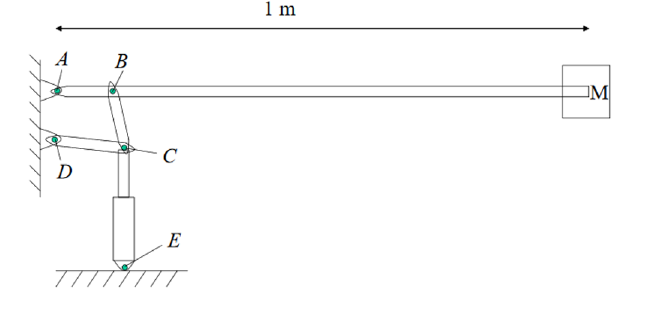
\includegraphics[width=\textwidth]{1_hydraulic_sim/BoomStructure.PNG}
    \caption{Hydraulic Boom Lift Structure}
    \label{fig:boom_structure}
\end{figure}


The control signal shown in Figure \ref{fig:hydraulic_cs} is used as input to the simulation of the hydraulic cylinder. The control signal represents an approximate square wave profile. It stays at a neutral voltage of 0 until 0.2 seconds into the simulation. At 0.2 seconds, the control signal is at its maximum of 10 volts for 0.4 seconds. Then it falls to become proportionally negative at 0.7 seconds. After another 0.4 seconds elapsed, the signal returns to the neural position of 0 volts begenning at 1.1 seconds.

\begin{figure}[H]
        %\centering
    %% Creator: Matplotlib, PGF backend
%%
%% To include the figure in your LaTeX document, write
%%   \input{<filename>.pgf}
%%
%% Make sure the required packages are loaded in your preamble
%%   \usepackage{pgf}
%%
%% Also ensure that all the required font packages are loaded; for instance,
%% the lmodern package is sometimes necessary when using math font.
%%   \usepackage{lmodern}
%%
%% Figures using additional raster images can only be included by \input if
%% they are in the same directory as the main LaTeX file. For loading figures
%% from other directories you can use the `import` package
%%   \usepackage{import}
%%
%% and then include the figures with
%%   \import{<path to file>}{<filename>.pgf}
%%
%% Matplotlib used the following preamble
%%
\begingroup%
\makeatletter%
\begin{pgfpicture}%
\pgfpathrectangle{\pgfpointorigin}{\pgfqpoint{6.000000in}{4.000000in}}%
\pgfusepath{use as bounding box, clip}%
\begin{pgfscope}%
\pgfsetbuttcap%
\pgfsetmiterjoin%
\pgfsetlinewidth{0.000000pt}%
\definecolor{currentstroke}{rgb}{1.000000,1.000000,1.000000}%
\pgfsetstrokecolor{currentstroke}%
\pgfsetstrokeopacity{0.000000}%
\pgfsetdash{}{0pt}%
\pgfpathmoveto{\pgfqpoint{0.000000in}{0.000000in}}%
\pgfpathlineto{\pgfqpoint{6.000000in}{0.000000in}}%
\pgfpathlineto{\pgfqpoint{6.000000in}{4.000000in}}%
\pgfpathlineto{\pgfqpoint{0.000000in}{4.000000in}}%
\pgfpathlineto{\pgfqpoint{0.000000in}{0.000000in}}%
\pgfpathclose%
\pgfusepath{}%
\end{pgfscope}%
\begin{pgfscope}%
\pgfsetbuttcap%
\pgfsetmiterjoin%
\definecolor{currentfill}{rgb}{1.000000,1.000000,1.000000}%
\pgfsetfillcolor{currentfill}%
\pgfsetlinewidth{0.000000pt}%
\definecolor{currentstroke}{rgb}{0.000000,0.000000,0.000000}%
\pgfsetstrokecolor{currentstroke}%
\pgfsetstrokeopacity{0.000000}%
\pgfsetdash{}{0pt}%
\pgfpathmoveto{\pgfqpoint{0.750000in}{0.500000in}}%
\pgfpathlineto{\pgfqpoint{5.400000in}{0.500000in}}%
\pgfpathlineto{\pgfqpoint{5.400000in}{3.520000in}}%
\pgfpathlineto{\pgfqpoint{0.750000in}{3.520000in}}%
\pgfpathlineto{\pgfqpoint{0.750000in}{0.500000in}}%
\pgfpathclose%
\pgfusepath{fill}%
\end{pgfscope}%
\begin{pgfscope}%
\pgfsetbuttcap%
\pgfsetroundjoin%
\definecolor{currentfill}{rgb}{0.000000,0.000000,0.000000}%
\pgfsetfillcolor{currentfill}%
\pgfsetlinewidth{0.803000pt}%
\definecolor{currentstroke}{rgb}{0.000000,0.000000,0.000000}%
\pgfsetstrokecolor{currentstroke}%
\pgfsetdash{}{0pt}%
\pgfsys@defobject{currentmarker}{\pgfqpoint{0.000000in}{-0.048611in}}{\pgfqpoint{0.000000in}{0.000000in}}{%
\pgfpathmoveto{\pgfqpoint{0.000000in}{0.000000in}}%
\pgfpathlineto{\pgfqpoint{0.000000in}{-0.048611in}}%
\pgfusepath{stroke,fill}%
}%
\begin{pgfscope}%
\pgfsys@transformshift{0.961364in}{0.500000in}%
\pgfsys@useobject{currentmarker}{}%
\end{pgfscope}%
\end{pgfscope}%
\begin{pgfscope}%
\definecolor{textcolor}{rgb}{0.000000,0.000000,0.000000}%
\pgfsetstrokecolor{textcolor}%
\pgfsetfillcolor{textcolor}%
\pgftext[x=0.961364in,y=0.402778in,,top]{\color{textcolor}\rmfamily\fontsize{10.000000}{12.000000}\selectfont \(\displaystyle {0.0}\)}%
\end{pgfscope}%
\begin{pgfscope}%
\pgfsetbuttcap%
\pgfsetroundjoin%
\definecolor{currentfill}{rgb}{0.000000,0.000000,0.000000}%
\pgfsetfillcolor{currentfill}%
\pgfsetlinewidth{0.803000pt}%
\definecolor{currentstroke}{rgb}{0.000000,0.000000,0.000000}%
\pgfsetstrokecolor{currentstroke}%
\pgfsetdash{}{0pt}%
\pgfsys@defobject{currentmarker}{\pgfqpoint{0.000000in}{-0.048611in}}{\pgfqpoint{0.000000in}{0.000000in}}{%
\pgfpathmoveto{\pgfqpoint{0.000000in}{0.000000in}}%
\pgfpathlineto{\pgfqpoint{0.000000in}{-0.048611in}}%
\pgfusepath{stroke,fill}%
}%
\begin{pgfscope}%
\pgfsys@transformshift{1.525000in}{0.500000in}%
\pgfsys@useobject{currentmarker}{}%
\end{pgfscope}%
\end{pgfscope}%
\begin{pgfscope}%
\definecolor{textcolor}{rgb}{0.000000,0.000000,0.000000}%
\pgfsetstrokecolor{textcolor}%
\pgfsetfillcolor{textcolor}%
\pgftext[x=1.525000in,y=0.402778in,,top]{\color{textcolor}\rmfamily\fontsize{10.000000}{12.000000}\selectfont \(\displaystyle {0.2}\)}%
\end{pgfscope}%
\begin{pgfscope}%
\pgfsetbuttcap%
\pgfsetroundjoin%
\definecolor{currentfill}{rgb}{0.000000,0.000000,0.000000}%
\pgfsetfillcolor{currentfill}%
\pgfsetlinewidth{0.803000pt}%
\definecolor{currentstroke}{rgb}{0.000000,0.000000,0.000000}%
\pgfsetstrokecolor{currentstroke}%
\pgfsetdash{}{0pt}%
\pgfsys@defobject{currentmarker}{\pgfqpoint{0.000000in}{-0.048611in}}{\pgfqpoint{0.000000in}{0.000000in}}{%
\pgfpathmoveto{\pgfqpoint{0.000000in}{0.000000in}}%
\pgfpathlineto{\pgfqpoint{0.000000in}{-0.048611in}}%
\pgfusepath{stroke,fill}%
}%
\begin{pgfscope}%
\pgfsys@transformshift{2.088636in}{0.500000in}%
\pgfsys@useobject{currentmarker}{}%
\end{pgfscope}%
\end{pgfscope}%
\begin{pgfscope}%
\definecolor{textcolor}{rgb}{0.000000,0.000000,0.000000}%
\pgfsetstrokecolor{textcolor}%
\pgfsetfillcolor{textcolor}%
\pgftext[x=2.088636in,y=0.402778in,,top]{\color{textcolor}\rmfamily\fontsize{10.000000}{12.000000}\selectfont \(\displaystyle {0.4}\)}%
\end{pgfscope}%
\begin{pgfscope}%
\pgfsetbuttcap%
\pgfsetroundjoin%
\definecolor{currentfill}{rgb}{0.000000,0.000000,0.000000}%
\pgfsetfillcolor{currentfill}%
\pgfsetlinewidth{0.803000pt}%
\definecolor{currentstroke}{rgb}{0.000000,0.000000,0.000000}%
\pgfsetstrokecolor{currentstroke}%
\pgfsetdash{}{0pt}%
\pgfsys@defobject{currentmarker}{\pgfqpoint{0.000000in}{-0.048611in}}{\pgfqpoint{0.000000in}{0.000000in}}{%
\pgfpathmoveto{\pgfqpoint{0.000000in}{0.000000in}}%
\pgfpathlineto{\pgfqpoint{0.000000in}{-0.048611in}}%
\pgfusepath{stroke,fill}%
}%
\begin{pgfscope}%
\pgfsys@transformshift{2.652273in}{0.500000in}%
\pgfsys@useobject{currentmarker}{}%
\end{pgfscope}%
\end{pgfscope}%
\begin{pgfscope}%
\definecolor{textcolor}{rgb}{0.000000,0.000000,0.000000}%
\pgfsetstrokecolor{textcolor}%
\pgfsetfillcolor{textcolor}%
\pgftext[x=2.652273in,y=0.402778in,,top]{\color{textcolor}\rmfamily\fontsize{10.000000}{12.000000}\selectfont \(\displaystyle {0.6}\)}%
\end{pgfscope}%
\begin{pgfscope}%
\pgfsetbuttcap%
\pgfsetroundjoin%
\definecolor{currentfill}{rgb}{0.000000,0.000000,0.000000}%
\pgfsetfillcolor{currentfill}%
\pgfsetlinewidth{0.803000pt}%
\definecolor{currentstroke}{rgb}{0.000000,0.000000,0.000000}%
\pgfsetstrokecolor{currentstroke}%
\pgfsetdash{}{0pt}%
\pgfsys@defobject{currentmarker}{\pgfqpoint{0.000000in}{-0.048611in}}{\pgfqpoint{0.000000in}{0.000000in}}{%
\pgfpathmoveto{\pgfqpoint{0.000000in}{0.000000in}}%
\pgfpathlineto{\pgfqpoint{0.000000in}{-0.048611in}}%
\pgfusepath{stroke,fill}%
}%
\begin{pgfscope}%
\pgfsys@transformshift{3.215909in}{0.500000in}%
\pgfsys@useobject{currentmarker}{}%
\end{pgfscope}%
\end{pgfscope}%
\begin{pgfscope}%
\definecolor{textcolor}{rgb}{0.000000,0.000000,0.000000}%
\pgfsetstrokecolor{textcolor}%
\pgfsetfillcolor{textcolor}%
\pgftext[x=3.215909in,y=0.402778in,,top]{\color{textcolor}\rmfamily\fontsize{10.000000}{12.000000}\selectfont \(\displaystyle {0.8}\)}%
\end{pgfscope}%
\begin{pgfscope}%
\pgfsetbuttcap%
\pgfsetroundjoin%
\definecolor{currentfill}{rgb}{0.000000,0.000000,0.000000}%
\pgfsetfillcolor{currentfill}%
\pgfsetlinewidth{0.803000pt}%
\definecolor{currentstroke}{rgb}{0.000000,0.000000,0.000000}%
\pgfsetstrokecolor{currentstroke}%
\pgfsetdash{}{0pt}%
\pgfsys@defobject{currentmarker}{\pgfqpoint{0.000000in}{-0.048611in}}{\pgfqpoint{0.000000in}{0.000000in}}{%
\pgfpathmoveto{\pgfqpoint{0.000000in}{0.000000in}}%
\pgfpathlineto{\pgfqpoint{0.000000in}{-0.048611in}}%
\pgfusepath{stroke,fill}%
}%
\begin{pgfscope}%
\pgfsys@transformshift{3.779545in}{0.500000in}%
\pgfsys@useobject{currentmarker}{}%
\end{pgfscope}%
\end{pgfscope}%
\begin{pgfscope}%
\definecolor{textcolor}{rgb}{0.000000,0.000000,0.000000}%
\pgfsetstrokecolor{textcolor}%
\pgfsetfillcolor{textcolor}%
\pgftext[x=3.779545in,y=0.402778in,,top]{\color{textcolor}\rmfamily\fontsize{10.000000}{12.000000}\selectfont \(\displaystyle {1.0}\)}%
\end{pgfscope}%
\begin{pgfscope}%
\pgfsetbuttcap%
\pgfsetroundjoin%
\definecolor{currentfill}{rgb}{0.000000,0.000000,0.000000}%
\pgfsetfillcolor{currentfill}%
\pgfsetlinewidth{0.803000pt}%
\definecolor{currentstroke}{rgb}{0.000000,0.000000,0.000000}%
\pgfsetstrokecolor{currentstroke}%
\pgfsetdash{}{0pt}%
\pgfsys@defobject{currentmarker}{\pgfqpoint{0.000000in}{-0.048611in}}{\pgfqpoint{0.000000in}{0.000000in}}{%
\pgfpathmoveto{\pgfqpoint{0.000000in}{0.000000in}}%
\pgfpathlineto{\pgfqpoint{0.000000in}{-0.048611in}}%
\pgfusepath{stroke,fill}%
}%
\begin{pgfscope}%
\pgfsys@transformshift{4.343182in}{0.500000in}%
\pgfsys@useobject{currentmarker}{}%
\end{pgfscope}%
\end{pgfscope}%
\begin{pgfscope}%
\definecolor{textcolor}{rgb}{0.000000,0.000000,0.000000}%
\pgfsetstrokecolor{textcolor}%
\pgfsetfillcolor{textcolor}%
\pgftext[x=4.343182in,y=0.402778in,,top]{\color{textcolor}\rmfamily\fontsize{10.000000}{12.000000}\selectfont \(\displaystyle {1.2}\)}%
\end{pgfscope}%
\begin{pgfscope}%
\pgfsetbuttcap%
\pgfsetroundjoin%
\definecolor{currentfill}{rgb}{0.000000,0.000000,0.000000}%
\pgfsetfillcolor{currentfill}%
\pgfsetlinewidth{0.803000pt}%
\definecolor{currentstroke}{rgb}{0.000000,0.000000,0.000000}%
\pgfsetstrokecolor{currentstroke}%
\pgfsetdash{}{0pt}%
\pgfsys@defobject{currentmarker}{\pgfqpoint{0.000000in}{-0.048611in}}{\pgfqpoint{0.000000in}{0.000000in}}{%
\pgfpathmoveto{\pgfqpoint{0.000000in}{0.000000in}}%
\pgfpathlineto{\pgfqpoint{0.000000in}{-0.048611in}}%
\pgfusepath{stroke,fill}%
}%
\begin{pgfscope}%
\pgfsys@transformshift{4.906818in}{0.500000in}%
\pgfsys@useobject{currentmarker}{}%
\end{pgfscope}%
\end{pgfscope}%
\begin{pgfscope}%
\definecolor{textcolor}{rgb}{0.000000,0.000000,0.000000}%
\pgfsetstrokecolor{textcolor}%
\pgfsetfillcolor{textcolor}%
\pgftext[x=4.906818in,y=0.402778in,,top]{\color{textcolor}\rmfamily\fontsize{10.000000}{12.000000}\selectfont \(\displaystyle {1.4}\)}%
\end{pgfscope}%
\begin{pgfscope}%
\definecolor{textcolor}{rgb}{0.000000,0.000000,0.000000}%
\pgfsetstrokecolor{textcolor}%
\pgfsetfillcolor{textcolor}%
\pgftext[x=3.075000in,y=0.223766in,,top]{\color{textcolor}\rmfamily\fontsize{10.000000}{12.000000}\selectfont Time (s)}%
\end{pgfscope}%
\begin{pgfscope}%
\pgfsetbuttcap%
\pgfsetroundjoin%
\definecolor{currentfill}{rgb}{0.000000,0.000000,0.000000}%
\pgfsetfillcolor{currentfill}%
\pgfsetlinewidth{0.803000pt}%
\definecolor{currentstroke}{rgb}{0.000000,0.000000,0.000000}%
\pgfsetstrokecolor{currentstroke}%
\pgfsetdash{}{0pt}%
\pgfsys@defobject{currentmarker}{\pgfqpoint{-0.048611in}{0.000000in}}{\pgfqpoint{-0.000000in}{0.000000in}}{%
\pgfpathmoveto{\pgfqpoint{-0.000000in}{0.000000in}}%
\pgfpathlineto{\pgfqpoint{-0.048611in}{0.000000in}}%
\pgfusepath{stroke,fill}%
}%
\begin{pgfscope}%
\pgfsys@transformshift{0.750000in}{0.637273in}%
\pgfsys@useobject{currentmarker}{}%
\end{pgfscope}%
\end{pgfscope}%
\begin{pgfscope}%
\definecolor{textcolor}{rgb}{0.000000,0.000000,0.000000}%
\pgfsetstrokecolor{textcolor}%
\pgfsetfillcolor{textcolor}%
\pgftext[x=0.297838in, y=0.589047in, left, base]{\color{textcolor}\rmfamily\fontsize{10.000000}{12.000000}\selectfont \(\displaystyle {\ensuremath{-}10.0}\)}%
\end{pgfscope}%
\begin{pgfscope}%
\pgfsetbuttcap%
\pgfsetroundjoin%
\definecolor{currentfill}{rgb}{0.000000,0.000000,0.000000}%
\pgfsetfillcolor{currentfill}%
\pgfsetlinewidth{0.803000pt}%
\definecolor{currentstroke}{rgb}{0.000000,0.000000,0.000000}%
\pgfsetstrokecolor{currentstroke}%
\pgfsetdash{}{0pt}%
\pgfsys@defobject{currentmarker}{\pgfqpoint{-0.048611in}{0.000000in}}{\pgfqpoint{-0.000000in}{0.000000in}}{%
\pgfpathmoveto{\pgfqpoint{-0.000000in}{0.000000in}}%
\pgfpathlineto{\pgfqpoint{-0.048611in}{0.000000in}}%
\pgfusepath{stroke,fill}%
}%
\begin{pgfscope}%
\pgfsys@transformshift{0.750000in}{0.980455in}%
\pgfsys@useobject{currentmarker}{}%
\end{pgfscope}%
\end{pgfscope}%
\begin{pgfscope}%
\definecolor{textcolor}{rgb}{0.000000,0.000000,0.000000}%
\pgfsetstrokecolor{textcolor}%
\pgfsetfillcolor{textcolor}%
\pgftext[x=0.367283in, y=0.932229in, left, base]{\color{textcolor}\rmfamily\fontsize{10.000000}{12.000000}\selectfont \(\displaystyle {\ensuremath{-}7.5}\)}%
\end{pgfscope}%
\begin{pgfscope}%
\pgfsetbuttcap%
\pgfsetroundjoin%
\definecolor{currentfill}{rgb}{0.000000,0.000000,0.000000}%
\pgfsetfillcolor{currentfill}%
\pgfsetlinewidth{0.803000pt}%
\definecolor{currentstroke}{rgb}{0.000000,0.000000,0.000000}%
\pgfsetstrokecolor{currentstroke}%
\pgfsetdash{}{0pt}%
\pgfsys@defobject{currentmarker}{\pgfqpoint{-0.048611in}{0.000000in}}{\pgfqpoint{-0.000000in}{0.000000in}}{%
\pgfpathmoveto{\pgfqpoint{-0.000000in}{0.000000in}}%
\pgfpathlineto{\pgfqpoint{-0.048611in}{0.000000in}}%
\pgfusepath{stroke,fill}%
}%
\begin{pgfscope}%
\pgfsys@transformshift{0.750000in}{1.323636in}%
\pgfsys@useobject{currentmarker}{}%
\end{pgfscope}%
\end{pgfscope}%
\begin{pgfscope}%
\definecolor{textcolor}{rgb}{0.000000,0.000000,0.000000}%
\pgfsetstrokecolor{textcolor}%
\pgfsetfillcolor{textcolor}%
\pgftext[x=0.367283in, y=1.275411in, left, base]{\color{textcolor}\rmfamily\fontsize{10.000000}{12.000000}\selectfont \(\displaystyle {\ensuremath{-}5.0}\)}%
\end{pgfscope}%
\begin{pgfscope}%
\pgfsetbuttcap%
\pgfsetroundjoin%
\definecolor{currentfill}{rgb}{0.000000,0.000000,0.000000}%
\pgfsetfillcolor{currentfill}%
\pgfsetlinewidth{0.803000pt}%
\definecolor{currentstroke}{rgb}{0.000000,0.000000,0.000000}%
\pgfsetstrokecolor{currentstroke}%
\pgfsetdash{}{0pt}%
\pgfsys@defobject{currentmarker}{\pgfqpoint{-0.048611in}{0.000000in}}{\pgfqpoint{-0.000000in}{0.000000in}}{%
\pgfpathmoveto{\pgfqpoint{-0.000000in}{0.000000in}}%
\pgfpathlineto{\pgfqpoint{-0.048611in}{0.000000in}}%
\pgfusepath{stroke,fill}%
}%
\begin{pgfscope}%
\pgfsys@transformshift{0.750000in}{1.666818in}%
\pgfsys@useobject{currentmarker}{}%
\end{pgfscope}%
\end{pgfscope}%
\begin{pgfscope}%
\definecolor{textcolor}{rgb}{0.000000,0.000000,0.000000}%
\pgfsetstrokecolor{textcolor}%
\pgfsetfillcolor{textcolor}%
\pgftext[x=0.367283in, y=1.618593in, left, base]{\color{textcolor}\rmfamily\fontsize{10.000000}{12.000000}\selectfont \(\displaystyle {\ensuremath{-}2.5}\)}%
\end{pgfscope}%
\begin{pgfscope}%
\pgfsetbuttcap%
\pgfsetroundjoin%
\definecolor{currentfill}{rgb}{0.000000,0.000000,0.000000}%
\pgfsetfillcolor{currentfill}%
\pgfsetlinewidth{0.803000pt}%
\definecolor{currentstroke}{rgb}{0.000000,0.000000,0.000000}%
\pgfsetstrokecolor{currentstroke}%
\pgfsetdash{}{0pt}%
\pgfsys@defobject{currentmarker}{\pgfqpoint{-0.048611in}{0.000000in}}{\pgfqpoint{-0.000000in}{0.000000in}}{%
\pgfpathmoveto{\pgfqpoint{-0.000000in}{0.000000in}}%
\pgfpathlineto{\pgfqpoint{-0.048611in}{0.000000in}}%
\pgfusepath{stroke,fill}%
}%
\begin{pgfscope}%
\pgfsys@transformshift{0.750000in}{2.010000in}%
\pgfsys@useobject{currentmarker}{}%
\end{pgfscope}%
\end{pgfscope}%
\begin{pgfscope}%
\definecolor{textcolor}{rgb}{0.000000,0.000000,0.000000}%
\pgfsetstrokecolor{textcolor}%
\pgfsetfillcolor{textcolor}%
\pgftext[x=0.475308in, y=1.961775in, left, base]{\color{textcolor}\rmfamily\fontsize{10.000000}{12.000000}\selectfont \(\displaystyle {0.0}\)}%
\end{pgfscope}%
\begin{pgfscope}%
\pgfsetbuttcap%
\pgfsetroundjoin%
\definecolor{currentfill}{rgb}{0.000000,0.000000,0.000000}%
\pgfsetfillcolor{currentfill}%
\pgfsetlinewidth{0.803000pt}%
\definecolor{currentstroke}{rgb}{0.000000,0.000000,0.000000}%
\pgfsetstrokecolor{currentstroke}%
\pgfsetdash{}{0pt}%
\pgfsys@defobject{currentmarker}{\pgfqpoint{-0.048611in}{0.000000in}}{\pgfqpoint{-0.000000in}{0.000000in}}{%
\pgfpathmoveto{\pgfqpoint{-0.000000in}{0.000000in}}%
\pgfpathlineto{\pgfqpoint{-0.048611in}{0.000000in}}%
\pgfusepath{stroke,fill}%
}%
\begin{pgfscope}%
\pgfsys@transformshift{0.750000in}{2.353182in}%
\pgfsys@useobject{currentmarker}{}%
\end{pgfscope}%
\end{pgfscope}%
\begin{pgfscope}%
\definecolor{textcolor}{rgb}{0.000000,0.000000,0.000000}%
\pgfsetstrokecolor{textcolor}%
\pgfsetfillcolor{textcolor}%
\pgftext[x=0.475308in, y=2.304957in, left, base]{\color{textcolor}\rmfamily\fontsize{10.000000}{12.000000}\selectfont \(\displaystyle {2.5}\)}%
\end{pgfscope}%
\begin{pgfscope}%
\pgfsetbuttcap%
\pgfsetroundjoin%
\definecolor{currentfill}{rgb}{0.000000,0.000000,0.000000}%
\pgfsetfillcolor{currentfill}%
\pgfsetlinewidth{0.803000pt}%
\definecolor{currentstroke}{rgb}{0.000000,0.000000,0.000000}%
\pgfsetstrokecolor{currentstroke}%
\pgfsetdash{}{0pt}%
\pgfsys@defobject{currentmarker}{\pgfqpoint{-0.048611in}{0.000000in}}{\pgfqpoint{-0.000000in}{0.000000in}}{%
\pgfpathmoveto{\pgfqpoint{-0.000000in}{0.000000in}}%
\pgfpathlineto{\pgfqpoint{-0.048611in}{0.000000in}}%
\pgfusepath{stroke,fill}%
}%
\begin{pgfscope}%
\pgfsys@transformshift{0.750000in}{2.696364in}%
\pgfsys@useobject{currentmarker}{}%
\end{pgfscope}%
\end{pgfscope}%
\begin{pgfscope}%
\definecolor{textcolor}{rgb}{0.000000,0.000000,0.000000}%
\pgfsetstrokecolor{textcolor}%
\pgfsetfillcolor{textcolor}%
\pgftext[x=0.475308in, y=2.648138in, left, base]{\color{textcolor}\rmfamily\fontsize{10.000000}{12.000000}\selectfont \(\displaystyle {5.0}\)}%
\end{pgfscope}%
\begin{pgfscope}%
\pgfsetbuttcap%
\pgfsetroundjoin%
\definecolor{currentfill}{rgb}{0.000000,0.000000,0.000000}%
\pgfsetfillcolor{currentfill}%
\pgfsetlinewidth{0.803000pt}%
\definecolor{currentstroke}{rgb}{0.000000,0.000000,0.000000}%
\pgfsetstrokecolor{currentstroke}%
\pgfsetdash{}{0pt}%
\pgfsys@defobject{currentmarker}{\pgfqpoint{-0.048611in}{0.000000in}}{\pgfqpoint{-0.000000in}{0.000000in}}{%
\pgfpathmoveto{\pgfqpoint{-0.000000in}{0.000000in}}%
\pgfpathlineto{\pgfqpoint{-0.048611in}{0.000000in}}%
\pgfusepath{stroke,fill}%
}%
\begin{pgfscope}%
\pgfsys@transformshift{0.750000in}{3.039545in}%
\pgfsys@useobject{currentmarker}{}%
\end{pgfscope}%
\end{pgfscope}%
\begin{pgfscope}%
\definecolor{textcolor}{rgb}{0.000000,0.000000,0.000000}%
\pgfsetstrokecolor{textcolor}%
\pgfsetfillcolor{textcolor}%
\pgftext[x=0.475308in, y=2.991320in, left, base]{\color{textcolor}\rmfamily\fontsize{10.000000}{12.000000}\selectfont \(\displaystyle {7.5}\)}%
\end{pgfscope}%
\begin{pgfscope}%
\pgfsetbuttcap%
\pgfsetroundjoin%
\definecolor{currentfill}{rgb}{0.000000,0.000000,0.000000}%
\pgfsetfillcolor{currentfill}%
\pgfsetlinewidth{0.803000pt}%
\definecolor{currentstroke}{rgb}{0.000000,0.000000,0.000000}%
\pgfsetstrokecolor{currentstroke}%
\pgfsetdash{}{0pt}%
\pgfsys@defobject{currentmarker}{\pgfqpoint{-0.048611in}{0.000000in}}{\pgfqpoint{-0.000000in}{0.000000in}}{%
\pgfpathmoveto{\pgfqpoint{-0.000000in}{0.000000in}}%
\pgfpathlineto{\pgfqpoint{-0.048611in}{0.000000in}}%
\pgfusepath{stroke,fill}%
}%
\begin{pgfscope}%
\pgfsys@transformshift{0.750000in}{3.382727in}%
\pgfsys@useobject{currentmarker}{}%
\end{pgfscope}%
\end{pgfscope}%
\begin{pgfscope}%
\definecolor{textcolor}{rgb}{0.000000,0.000000,0.000000}%
\pgfsetstrokecolor{textcolor}%
\pgfsetfillcolor{textcolor}%
\pgftext[x=0.405863in, y=3.334502in, left, base]{\color{textcolor}\rmfamily\fontsize{10.000000}{12.000000}\selectfont \(\displaystyle {10.0}\)}%
\end{pgfscope}%
\begin{pgfscope}%
\definecolor{textcolor}{rgb}{0.000000,0.000000,0.000000}%
\pgfsetstrokecolor{textcolor}%
\pgfsetfillcolor{textcolor}%
\pgftext[x=0.242283in,y=2.010000in,,bottom,rotate=90.000000]{\color{textcolor}\rmfamily\fontsize{10.000000}{12.000000}\selectfont Voltage (\(\displaystyle V\))}%
\end{pgfscope}%
\begin{pgfscope}%
\pgfpathrectangle{\pgfqpoint{0.750000in}{0.500000in}}{\pgfqpoint{4.650000in}{3.020000in}}%
\pgfusepath{clip}%
\pgfsetrectcap%
\pgfsetroundjoin%
\pgfsetlinewidth{1.505625pt}%
\definecolor{currentstroke}{rgb}{0.121569,0.466667,0.705882}%
\pgfsetstrokecolor{currentstroke}%
\pgfsetdash{}{0pt}%
\pgfpathmoveto{\pgfqpoint{0.961364in}{2.010000in}}%
\pgfpathlineto{\pgfqpoint{1.525156in}{2.011521in}}%
\pgfpathlineto{\pgfqpoint{1.665909in}{3.382727in}}%
\pgfpathlineto{\pgfqpoint{1.665909in}{3.382727in}}%
\pgfpathlineto{\pgfqpoint{2.652273in}{3.382727in}}%
\pgfpathlineto{\pgfqpoint{2.652273in}{3.382727in}}%
\pgfpathlineto{\pgfqpoint{2.934091in}{0.637273in}}%
\pgfpathlineto{\pgfqpoint{2.934091in}{0.637273in}}%
\pgfpathlineto{\pgfqpoint{3.920455in}{0.637273in}}%
\pgfpathlineto{\pgfqpoint{3.920455in}{0.637273in}}%
\pgfpathlineto{\pgfqpoint{4.062434in}{2.010001in}}%
\pgfpathlineto{\pgfqpoint{4.062434in}{2.010001in}}%
\pgfpathlineto{\pgfqpoint{5.188636in}{2.011445in}}%
\pgfpathlineto{\pgfqpoint{5.188636in}{2.011445in}}%
\pgfusepath{stroke}%
\end{pgfscope}%
\begin{pgfscope}%
\pgfsetrectcap%
\pgfsetmiterjoin%
\pgfsetlinewidth{0.803000pt}%
\definecolor{currentstroke}{rgb}{0.000000,0.000000,0.000000}%
\pgfsetstrokecolor{currentstroke}%
\pgfsetdash{}{0pt}%
\pgfpathmoveto{\pgfqpoint{0.750000in}{0.500000in}}%
\pgfpathlineto{\pgfqpoint{0.750000in}{3.520000in}}%
\pgfusepath{stroke}%
\end{pgfscope}%
\begin{pgfscope}%
\pgfsetrectcap%
\pgfsetmiterjoin%
\pgfsetlinewidth{0.803000pt}%
\definecolor{currentstroke}{rgb}{0.000000,0.000000,0.000000}%
\pgfsetstrokecolor{currentstroke}%
\pgfsetdash{}{0pt}%
\pgfpathmoveto{\pgfqpoint{5.400000in}{0.500000in}}%
\pgfpathlineto{\pgfqpoint{5.400000in}{3.520000in}}%
\pgfusepath{stroke}%
\end{pgfscope}%
\begin{pgfscope}%
\pgfsetrectcap%
\pgfsetmiterjoin%
\pgfsetlinewidth{0.803000pt}%
\definecolor{currentstroke}{rgb}{0.000000,0.000000,0.000000}%
\pgfsetstrokecolor{currentstroke}%
\pgfsetdash{}{0pt}%
\pgfpathmoveto{\pgfqpoint{0.750000in}{0.500000in}}%
\pgfpathlineto{\pgfqpoint{5.400000in}{0.500000in}}%
\pgfusepath{stroke}%
\end{pgfscope}%
\begin{pgfscope}%
\pgfsetrectcap%
\pgfsetmiterjoin%
\pgfsetlinewidth{0.803000pt}%
\definecolor{currentstroke}{rgb}{0.000000,0.000000,0.000000}%
\pgfsetstrokecolor{currentstroke}%
\pgfsetdash{}{0pt}%
\pgfpathmoveto{\pgfqpoint{0.750000in}{3.520000in}}%
\pgfpathlineto{\pgfqpoint{5.400000in}{3.520000in}}%
\pgfusepath{stroke}%
\end{pgfscope}%
\end{pgfpicture}%
\makeatother%
\endgroup%

    \caption{Hydraulic System Control Signal}
    \label{fig:hydraulic_cs}
\end{figure}

Figure \ref{fig:hydraulic_pos} shows the pressure for the system over time. Introducing a proportionally negative signal does not cause the end effector to return to its initial position. As the control signal is varied inversely, the position of the end effector only returns halfway to its initial position. This indicates the system exhibits a non-linear relationship between the control signal and the end effector position. The system experiences mild oscillation after coming to rest when the control signal is back to zero at the end of the simulation. To achieve predictable system response and reduce oscillation, a more complex control methodology would be required.

\begin{figure}[H]
        %\centering
    %% Creator: Matplotlib, PGF backend
%%
%% To include the figure in your LaTeX document, write
%%   \input{<filename>.pgf}
%%
%% Make sure the required packages are loaded in your preamble
%%   \usepackage{pgf}
%%
%% Also ensure that all the required font packages are loaded; for instance,
%% the lmodern package is sometimes necessary when using math font.
%%   \usepackage{lmodern}
%%
%% Figures using additional raster images can only be included by \input if
%% they are in the same directory as the main LaTeX file. For loading figures
%% from other directories you can use the `import` package
%%   \usepackage{import}
%%
%% and then include the figures with
%%   \import{<path to file>}{<filename>.pgf}
%%
%% Matplotlib used the following preamble
%%   \usepackage{fontspec}
%%   \setmainfont{DejaVuSerif.ttf}[Path=\detokenize{/Users/abeattie/miniconda/envs/masters-thesis/lib/python3.10/site-packages/matplotlib/mpl-data/fonts/ttf/}]
%%   \setsansfont{DejaVuSans.ttf}[Path=\detokenize{/Users/abeattie/miniconda/envs/masters-thesis/lib/python3.10/site-packages/matplotlib/mpl-data/fonts/ttf/}]
%%   \setmonofont{DejaVuSansMono.ttf}[Path=\detokenize{/Users/abeattie/miniconda/envs/masters-thesis/lib/python3.10/site-packages/matplotlib/mpl-data/fonts/ttf/}]
%%
\begingroup%
\makeatletter%
\begin{pgfpicture}%
\pgfpathrectangle{\pgfpointorigin}{\pgfqpoint{6.000000in}{4.000000in}}%
\pgfusepath{use as bounding box, clip}%
\begin{pgfscope}%
\pgfsetbuttcap%
\pgfsetmiterjoin%
\pgfsetlinewidth{0.000000pt}%
\definecolor{currentstroke}{rgb}{1.000000,1.000000,1.000000}%
\pgfsetstrokecolor{currentstroke}%
\pgfsetstrokeopacity{0.000000}%
\pgfsetdash{}{0pt}%
\pgfpathmoveto{\pgfqpoint{0.000000in}{0.000000in}}%
\pgfpathlineto{\pgfqpoint{6.000000in}{0.000000in}}%
\pgfpathlineto{\pgfqpoint{6.000000in}{4.000000in}}%
\pgfpathlineto{\pgfqpoint{0.000000in}{4.000000in}}%
\pgfpathlineto{\pgfqpoint{0.000000in}{0.000000in}}%
\pgfpathclose%
\pgfusepath{}%
\end{pgfscope}%
\end{pgfpicture}%
\makeatother%
\endgroup%

    \caption{Hydraulic Crane End Effector Position}
    \label{fig:hydraulic_pos}
\end{figure}

\subsubsection{Power Electronic Converter Dataset}
\label{ref_pec_dataset}

Transitioning from the conventional power systems to power electronics-dominated grids (PEDG) has increased demand for grid-forming converters (GFM) to facilitate operational reliability. GFMs have made significant progress in recent years % (as shown in Figure \ref{fig:sys})
to expedite stability under different grid conditions, but their operation during faults or large signal disturbances still remain a challenge.

Authors \cite{trainsient-stability-9523750} explain that GFMs handle a significantly smaller percentage of over-current (usually only 20\%) compared to synchronous generators (SGs) which can handle seven times their nominal current. This makes extreme fault detection and protection for GFMs critical while maintaining synchronization with the grid. Since the network infrastructure of power systems keeps expanding, it is important to identify these faults accurately under varying grid parameter uncertainties.

% \begin{figure}[H]
% 	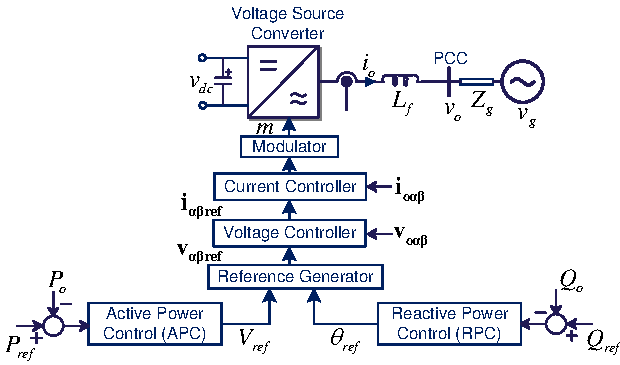
\includegraphics[width=\textwidth]{Images/GFMSchema.pdf}
% 	\caption{Main circuit and control system structure of a grid-forming converter.}
% 	\label{fig:sys}
% \end{figure}

Four faults are considered in the PEC dataset. This study examines the frequency [$f_c$] of the system throughout various fault conditions. Each fault has significantly different characteristics and magnitude. The faults exaimned in the study are explained in Table \ref{tab:pec_faults_table}.

\bigskip
\begin{longtable}{P{2cm} P{3.5cm} l}
\caption{PEC Dataset Classifications} \\
\toprule
\textbf{Fault} & \textbf{Description} & \textbf{Frequency Shape} \\
\midrule
\endfirsthead
\multicolumn{3}{c}%
{\tablename\ \thetable\ -- \textit{Continued from previous page}} \\
\hline
\textbf{Fault} & \textbf{Description} & \textbf{Frequency Shape} \\
\hline
\endhead
\hline \multicolumn{3}{r}{\textit{Continued on next page}} \\
\endfoot
\hline
\endlastfoot
    Line-to-Line (LL) Fault & This fault occurs when there is a short circuit between two conductors. & 
    \raisebox{-0.9\totalheight}{\resizebox{8cm}{!}{%% Creator: Matplotlib, PGF backend
%%
%% To include the figure in your LaTeX document, write
%%   \input{<filename>.pgf}
%%
%% Make sure the required packages are loaded in your preamble
%%   \usepackage{pgf}
%%
%% Also ensure that all the required font packages are loaded; for instance,
%% the lmodern package is sometimes necessary when using math font.
%%   \usepackage{lmodern}
%%
%% Figures using additional raster images can only be included by \input if
%% they are in the same directory as the main LaTeX file. For loading figures
%% from other directories you can use the `import` package
%%   \usepackage{import}
%%
%% and then include the figures with
%%   \import{<path to file>}{<filename>.pgf}
%%
%% Matplotlib used the following preamble
%%
\begingroup%
\makeatletter%
\begin{pgfpicture}%
\pgfpathrectangle{\pgfpointorigin}{\pgfqpoint{5.000000in}{4.000000in}}%
\pgfusepath{use as bounding box, clip}%
\begin{pgfscope}%
\pgfsetbuttcap%
\pgfsetmiterjoin%
\pgfsetlinewidth{0.000000pt}%
\definecolor{currentstroke}{rgb}{1.000000,1.000000,1.000000}%
\pgfsetstrokecolor{currentstroke}%
\pgfsetstrokeopacity{0.000000}%
\pgfsetdash{}{0pt}%
\pgfpathmoveto{\pgfqpoint{0.000000in}{0.000000in}}%
\pgfpathlineto{\pgfqpoint{5.000000in}{0.000000in}}%
\pgfpathlineto{\pgfqpoint{5.000000in}{4.000000in}}%
\pgfpathlineto{\pgfqpoint{0.000000in}{4.000000in}}%
\pgfpathlineto{\pgfqpoint{0.000000in}{0.000000in}}%
\pgfpathclose%
\pgfusepath{}%
\end{pgfscope}%
\begin{pgfscope}%
\pgfsetbuttcap%
\pgfsetmiterjoin%
\definecolor{currentfill}{rgb}{1.000000,1.000000,1.000000}%
\pgfsetfillcolor{currentfill}%
\pgfsetlinewidth{0.000000pt}%
\definecolor{currentstroke}{rgb}{0.000000,0.000000,0.000000}%
\pgfsetstrokecolor{currentstroke}%
\pgfsetstrokeopacity{0.000000}%
\pgfsetdash{}{0pt}%
\pgfpathmoveto{\pgfqpoint{0.625000in}{0.500000in}}%
\pgfpathlineto{\pgfqpoint{4.500000in}{0.500000in}}%
\pgfpathlineto{\pgfqpoint{4.500000in}{3.520000in}}%
\pgfpathlineto{\pgfqpoint{0.625000in}{3.520000in}}%
\pgfpathlineto{\pgfqpoint{0.625000in}{0.500000in}}%
\pgfpathclose%
\pgfusepath{fill}%
\end{pgfscope}%
\begin{pgfscope}%
\pgfsetbuttcap%
\pgfsetroundjoin%
\definecolor{currentfill}{rgb}{0.000000,0.000000,0.000000}%
\pgfsetfillcolor{currentfill}%
\pgfsetlinewidth{0.803000pt}%
\definecolor{currentstroke}{rgb}{0.000000,0.000000,0.000000}%
\pgfsetstrokecolor{currentstroke}%
\pgfsetdash{}{0pt}%
\pgfsys@defobject{currentmarker}{\pgfqpoint{0.000000in}{-0.048611in}}{\pgfqpoint{0.000000in}{0.000000in}}{%
\pgfpathmoveto{\pgfqpoint{0.000000in}{0.000000in}}%
\pgfpathlineto{\pgfqpoint{0.000000in}{-0.048611in}}%
\pgfusepath{stroke,fill}%
}%
\begin{pgfscope}%
\pgfsys@transformshift{0.801136in}{0.500000in}%
\pgfsys@useobject{currentmarker}{}%
\end{pgfscope}%
\end{pgfscope}%
\begin{pgfscope}%
\definecolor{textcolor}{rgb}{0.000000,0.000000,0.000000}%
\pgfsetstrokecolor{textcolor}%
\pgfsetfillcolor{textcolor}%
\pgftext[x=0.801136in,y=0.402778in,,top]{\color{textcolor}\rmfamily\fontsize{10.000000}{12.000000}\selectfont \(\displaystyle {40200}\)}%
\end{pgfscope}%
\begin{pgfscope}%
\pgfsetbuttcap%
\pgfsetroundjoin%
\definecolor{currentfill}{rgb}{0.000000,0.000000,0.000000}%
\pgfsetfillcolor{currentfill}%
\pgfsetlinewidth{0.803000pt}%
\definecolor{currentstroke}{rgb}{0.000000,0.000000,0.000000}%
\pgfsetstrokecolor{currentstroke}%
\pgfsetdash{}{0pt}%
\pgfsys@defobject{currentmarker}{\pgfqpoint{0.000000in}{-0.048611in}}{\pgfqpoint{0.000000in}{0.000000in}}{%
\pgfpathmoveto{\pgfqpoint{0.000000in}{0.000000in}}%
\pgfpathlineto{\pgfqpoint{0.000000in}{-0.048611in}}%
\pgfusepath{stroke,fill}%
}%
\begin{pgfscope}%
\pgfsys@transformshift{1.506387in}{0.500000in}%
\pgfsys@useobject{currentmarker}{}%
\end{pgfscope}%
\end{pgfscope}%
\begin{pgfscope}%
\definecolor{textcolor}{rgb}{0.000000,0.000000,0.000000}%
\pgfsetstrokecolor{textcolor}%
\pgfsetfillcolor{textcolor}%
\pgftext[x=1.506387in,y=0.402778in,,top]{\color{textcolor}\rmfamily\fontsize{10.000000}{12.000000}\selectfont \(\displaystyle {40400}\)}%
\end{pgfscope}%
\begin{pgfscope}%
\pgfsetbuttcap%
\pgfsetroundjoin%
\definecolor{currentfill}{rgb}{0.000000,0.000000,0.000000}%
\pgfsetfillcolor{currentfill}%
\pgfsetlinewidth{0.803000pt}%
\definecolor{currentstroke}{rgb}{0.000000,0.000000,0.000000}%
\pgfsetstrokecolor{currentstroke}%
\pgfsetdash{}{0pt}%
\pgfsys@defobject{currentmarker}{\pgfqpoint{0.000000in}{-0.048611in}}{\pgfqpoint{0.000000in}{0.000000in}}{%
\pgfpathmoveto{\pgfqpoint{0.000000in}{0.000000in}}%
\pgfpathlineto{\pgfqpoint{0.000000in}{-0.048611in}}%
\pgfusepath{stroke,fill}%
}%
\begin{pgfscope}%
\pgfsys@transformshift{2.211638in}{0.500000in}%
\pgfsys@useobject{currentmarker}{}%
\end{pgfscope}%
\end{pgfscope}%
\begin{pgfscope}%
\definecolor{textcolor}{rgb}{0.000000,0.000000,0.000000}%
\pgfsetstrokecolor{textcolor}%
\pgfsetfillcolor{textcolor}%
\pgftext[x=2.211638in,y=0.402778in,,top]{\color{textcolor}\rmfamily\fontsize{10.000000}{12.000000}\selectfont \(\displaystyle {40600}\)}%
\end{pgfscope}%
\begin{pgfscope}%
\pgfsetbuttcap%
\pgfsetroundjoin%
\definecolor{currentfill}{rgb}{0.000000,0.000000,0.000000}%
\pgfsetfillcolor{currentfill}%
\pgfsetlinewidth{0.803000pt}%
\definecolor{currentstroke}{rgb}{0.000000,0.000000,0.000000}%
\pgfsetstrokecolor{currentstroke}%
\pgfsetdash{}{0pt}%
\pgfsys@defobject{currentmarker}{\pgfqpoint{0.000000in}{-0.048611in}}{\pgfqpoint{0.000000in}{0.000000in}}{%
\pgfpathmoveto{\pgfqpoint{0.000000in}{0.000000in}}%
\pgfpathlineto{\pgfqpoint{0.000000in}{-0.048611in}}%
\pgfusepath{stroke,fill}%
}%
\begin{pgfscope}%
\pgfsys@transformshift{2.916888in}{0.500000in}%
\pgfsys@useobject{currentmarker}{}%
\end{pgfscope}%
\end{pgfscope}%
\begin{pgfscope}%
\definecolor{textcolor}{rgb}{0.000000,0.000000,0.000000}%
\pgfsetstrokecolor{textcolor}%
\pgfsetfillcolor{textcolor}%
\pgftext[x=2.916888in,y=0.402778in,,top]{\color{textcolor}\rmfamily\fontsize{10.000000}{12.000000}\selectfont \(\displaystyle {40800}\)}%
\end{pgfscope}%
\begin{pgfscope}%
\pgfsetbuttcap%
\pgfsetroundjoin%
\definecolor{currentfill}{rgb}{0.000000,0.000000,0.000000}%
\pgfsetfillcolor{currentfill}%
\pgfsetlinewidth{0.803000pt}%
\definecolor{currentstroke}{rgb}{0.000000,0.000000,0.000000}%
\pgfsetstrokecolor{currentstroke}%
\pgfsetdash{}{0pt}%
\pgfsys@defobject{currentmarker}{\pgfqpoint{0.000000in}{-0.048611in}}{\pgfqpoint{0.000000in}{0.000000in}}{%
\pgfpathmoveto{\pgfqpoint{0.000000in}{0.000000in}}%
\pgfpathlineto{\pgfqpoint{0.000000in}{-0.048611in}}%
\pgfusepath{stroke,fill}%
}%
\begin{pgfscope}%
\pgfsys@transformshift{3.622139in}{0.500000in}%
\pgfsys@useobject{currentmarker}{}%
\end{pgfscope}%
\end{pgfscope}%
\begin{pgfscope}%
\definecolor{textcolor}{rgb}{0.000000,0.000000,0.000000}%
\pgfsetstrokecolor{textcolor}%
\pgfsetfillcolor{textcolor}%
\pgftext[x=3.622139in,y=0.402778in,,top]{\color{textcolor}\rmfamily\fontsize{10.000000}{12.000000}\selectfont \(\displaystyle {41000}\)}%
\end{pgfscope}%
\begin{pgfscope}%
\pgfsetbuttcap%
\pgfsetroundjoin%
\definecolor{currentfill}{rgb}{0.000000,0.000000,0.000000}%
\pgfsetfillcolor{currentfill}%
\pgfsetlinewidth{0.803000pt}%
\definecolor{currentstroke}{rgb}{0.000000,0.000000,0.000000}%
\pgfsetstrokecolor{currentstroke}%
\pgfsetdash{}{0pt}%
\pgfsys@defobject{currentmarker}{\pgfqpoint{0.000000in}{-0.048611in}}{\pgfqpoint{0.000000in}{0.000000in}}{%
\pgfpathmoveto{\pgfqpoint{0.000000in}{0.000000in}}%
\pgfpathlineto{\pgfqpoint{0.000000in}{-0.048611in}}%
\pgfusepath{stroke,fill}%
}%
\begin{pgfscope}%
\pgfsys@transformshift{4.327390in}{0.500000in}%
\pgfsys@useobject{currentmarker}{}%
\end{pgfscope}%
\end{pgfscope}%
\begin{pgfscope}%
\definecolor{textcolor}{rgb}{0.000000,0.000000,0.000000}%
\pgfsetstrokecolor{textcolor}%
\pgfsetfillcolor{textcolor}%
\pgftext[x=4.327390in,y=0.402778in,,top]{\color{textcolor}\rmfamily\fontsize{10.000000}{12.000000}\selectfont \(\displaystyle {41200}\)}%
\end{pgfscope}%
\begin{pgfscope}%
\definecolor{textcolor}{rgb}{0.000000,0.000000,0.000000}%
\pgfsetstrokecolor{textcolor}%
\pgfsetfillcolor{textcolor}%
\pgftext[x=2.562500in,y=0.223766in,,top]{\color{textcolor}\rmfamily\fontsize{10.000000}{12.000000}\selectfont Time (s)}%
\end{pgfscope}%
\begin{pgfscope}%
\pgfsetbuttcap%
\pgfsetroundjoin%
\definecolor{currentfill}{rgb}{0.000000,0.000000,0.000000}%
\pgfsetfillcolor{currentfill}%
\pgfsetlinewidth{0.803000pt}%
\definecolor{currentstroke}{rgb}{0.000000,0.000000,0.000000}%
\pgfsetstrokecolor{currentstroke}%
\pgfsetdash{}{0pt}%
\pgfsys@defobject{currentmarker}{\pgfqpoint{-0.048611in}{0.000000in}}{\pgfqpoint{-0.000000in}{0.000000in}}{%
\pgfpathmoveto{\pgfqpoint{-0.000000in}{0.000000in}}%
\pgfpathlineto{\pgfqpoint{-0.048611in}{0.000000in}}%
\pgfusepath{stroke,fill}%
}%
\begin{pgfscope}%
\pgfsys@transformshift{0.625000in}{0.686723in}%
\pgfsys@useobject{currentmarker}{}%
\end{pgfscope}%
\end{pgfscope}%
\begin{pgfscope}%
\definecolor{textcolor}{rgb}{0.000000,0.000000,0.000000}%
\pgfsetstrokecolor{textcolor}%
\pgfsetfillcolor{textcolor}%
\pgftext[x=0.350308in, y=0.638498in, left, base]{\color{textcolor}\rmfamily\fontsize{10.000000}{12.000000}\selectfont \(\displaystyle {\ensuremath{-}7}\)}%
\end{pgfscope}%
\begin{pgfscope}%
\pgfsetbuttcap%
\pgfsetroundjoin%
\definecolor{currentfill}{rgb}{0.000000,0.000000,0.000000}%
\pgfsetfillcolor{currentfill}%
\pgfsetlinewidth{0.803000pt}%
\definecolor{currentstroke}{rgb}{0.000000,0.000000,0.000000}%
\pgfsetstrokecolor{currentstroke}%
\pgfsetdash{}{0pt}%
\pgfsys@defobject{currentmarker}{\pgfqpoint{-0.048611in}{0.000000in}}{\pgfqpoint{-0.000000in}{0.000000in}}{%
\pgfpathmoveto{\pgfqpoint{-0.000000in}{0.000000in}}%
\pgfpathlineto{\pgfqpoint{-0.048611in}{0.000000in}}%
\pgfusepath{stroke,fill}%
}%
\begin{pgfscope}%
\pgfsys@transformshift{0.625000in}{1.069135in}%
\pgfsys@useobject{currentmarker}{}%
\end{pgfscope}%
\end{pgfscope}%
\begin{pgfscope}%
\definecolor{textcolor}{rgb}{0.000000,0.000000,0.000000}%
\pgfsetstrokecolor{textcolor}%
\pgfsetfillcolor{textcolor}%
\pgftext[x=0.350308in, y=1.020910in, left, base]{\color{textcolor}\rmfamily\fontsize{10.000000}{12.000000}\selectfont \(\displaystyle {\ensuremath{-}6}\)}%
\end{pgfscope}%
\begin{pgfscope}%
\pgfsetbuttcap%
\pgfsetroundjoin%
\definecolor{currentfill}{rgb}{0.000000,0.000000,0.000000}%
\pgfsetfillcolor{currentfill}%
\pgfsetlinewidth{0.803000pt}%
\definecolor{currentstroke}{rgb}{0.000000,0.000000,0.000000}%
\pgfsetstrokecolor{currentstroke}%
\pgfsetdash{}{0pt}%
\pgfsys@defobject{currentmarker}{\pgfqpoint{-0.048611in}{0.000000in}}{\pgfqpoint{-0.000000in}{0.000000in}}{%
\pgfpathmoveto{\pgfqpoint{-0.000000in}{0.000000in}}%
\pgfpathlineto{\pgfqpoint{-0.048611in}{0.000000in}}%
\pgfusepath{stroke,fill}%
}%
\begin{pgfscope}%
\pgfsys@transformshift{0.625000in}{1.451547in}%
\pgfsys@useobject{currentmarker}{}%
\end{pgfscope}%
\end{pgfscope}%
\begin{pgfscope}%
\definecolor{textcolor}{rgb}{0.000000,0.000000,0.000000}%
\pgfsetstrokecolor{textcolor}%
\pgfsetfillcolor{textcolor}%
\pgftext[x=0.350308in, y=1.403322in, left, base]{\color{textcolor}\rmfamily\fontsize{10.000000}{12.000000}\selectfont \(\displaystyle {\ensuremath{-}5}\)}%
\end{pgfscope}%
\begin{pgfscope}%
\pgfsetbuttcap%
\pgfsetroundjoin%
\definecolor{currentfill}{rgb}{0.000000,0.000000,0.000000}%
\pgfsetfillcolor{currentfill}%
\pgfsetlinewidth{0.803000pt}%
\definecolor{currentstroke}{rgb}{0.000000,0.000000,0.000000}%
\pgfsetstrokecolor{currentstroke}%
\pgfsetdash{}{0pt}%
\pgfsys@defobject{currentmarker}{\pgfqpoint{-0.048611in}{0.000000in}}{\pgfqpoint{-0.000000in}{0.000000in}}{%
\pgfpathmoveto{\pgfqpoint{-0.000000in}{0.000000in}}%
\pgfpathlineto{\pgfqpoint{-0.048611in}{0.000000in}}%
\pgfusepath{stroke,fill}%
}%
\begin{pgfscope}%
\pgfsys@transformshift{0.625000in}{1.833959in}%
\pgfsys@useobject{currentmarker}{}%
\end{pgfscope}%
\end{pgfscope}%
\begin{pgfscope}%
\definecolor{textcolor}{rgb}{0.000000,0.000000,0.000000}%
\pgfsetstrokecolor{textcolor}%
\pgfsetfillcolor{textcolor}%
\pgftext[x=0.350308in, y=1.785734in, left, base]{\color{textcolor}\rmfamily\fontsize{10.000000}{12.000000}\selectfont \(\displaystyle {\ensuremath{-}4}\)}%
\end{pgfscope}%
\begin{pgfscope}%
\pgfsetbuttcap%
\pgfsetroundjoin%
\definecolor{currentfill}{rgb}{0.000000,0.000000,0.000000}%
\pgfsetfillcolor{currentfill}%
\pgfsetlinewidth{0.803000pt}%
\definecolor{currentstroke}{rgb}{0.000000,0.000000,0.000000}%
\pgfsetstrokecolor{currentstroke}%
\pgfsetdash{}{0pt}%
\pgfsys@defobject{currentmarker}{\pgfqpoint{-0.048611in}{0.000000in}}{\pgfqpoint{-0.000000in}{0.000000in}}{%
\pgfpathmoveto{\pgfqpoint{-0.000000in}{0.000000in}}%
\pgfpathlineto{\pgfqpoint{-0.048611in}{0.000000in}}%
\pgfusepath{stroke,fill}%
}%
\begin{pgfscope}%
\pgfsys@transformshift{0.625000in}{2.216371in}%
\pgfsys@useobject{currentmarker}{}%
\end{pgfscope}%
\end{pgfscope}%
\begin{pgfscope}%
\definecolor{textcolor}{rgb}{0.000000,0.000000,0.000000}%
\pgfsetstrokecolor{textcolor}%
\pgfsetfillcolor{textcolor}%
\pgftext[x=0.350308in, y=2.168146in, left, base]{\color{textcolor}\rmfamily\fontsize{10.000000}{12.000000}\selectfont \(\displaystyle {\ensuremath{-}3}\)}%
\end{pgfscope}%
\begin{pgfscope}%
\pgfsetbuttcap%
\pgfsetroundjoin%
\definecolor{currentfill}{rgb}{0.000000,0.000000,0.000000}%
\pgfsetfillcolor{currentfill}%
\pgfsetlinewidth{0.803000pt}%
\definecolor{currentstroke}{rgb}{0.000000,0.000000,0.000000}%
\pgfsetstrokecolor{currentstroke}%
\pgfsetdash{}{0pt}%
\pgfsys@defobject{currentmarker}{\pgfqpoint{-0.048611in}{0.000000in}}{\pgfqpoint{-0.000000in}{0.000000in}}{%
\pgfpathmoveto{\pgfqpoint{-0.000000in}{0.000000in}}%
\pgfpathlineto{\pgfqpoint{-0.048611in}{0.000000in}}%
\pgfusepath{stroke,fill}%
}%
\begin{pgfscope}%
\pgfsys@transformshift{0.625000in}{2.598783in}%
\pgfsys@useobject{currentmarker}{}%
\end{pgfscope}%
\end{pgfscope}%
\begin{pgfscope}%
\definecolor{textcolor}{rgb}{0.000000,0.000000,0.000000}%
\pgfsetstrokecolor{textcolor}%
\pgfsetfillcolor{textcolor}%
\pgftext[x=0.350308in, y=2.550558in, left, base]{\color{textcolor}\rmfamily\fontsize{10.000000}{12.000000}\selectfont \(\displaystyle {\ensuremath{-}2}\)}%
\end{pgfscope}%
\begin{pgfscope}%
\pgfsetbuttcap%
\pgfsetroundjoin%
\definecolor{currentfill}{rgb}{0.000000,0.000000,0.000000}%
\pgfsetfillcolor{currentfill}%
\pgfsetlinewidth{0.803000pt}%
\definecolor{currentstroke}{rgb}{0.000000,0.000000,0.000000}%
\pgfsetstrokecolor{currentstroke}%
\pgfsetdash{}{0pt}%
\pgfsys@defobject{currentmarker}{\pgfqpoint{-0.048611in}{0.000000in}}{\pgfqpoint{-0.000000in}{0.000000in}}{%
\pgfpathmoveto{\pgfqpoint{-0.000000in}{0.000000in}}%
\pgfpathlineto{\pgfqpoint{-0.048611in}{0.000000in}}%
\pgfusepath{stroke,fill}%
}%
\begin{pgfscope}%
\pgfsys@transformshift{0.625000in}{2.981195in}%
\pgfsys@useobject{currentmarker}{}%
\end{pgfscope}%
\end{pgfscope}%
\begin{pgfscope}%
\definecolor{textcolor}{rgb}{0.000000,0.000000,0.000000}%
\pgfsetstrokecolor{textcolor}%
\pgfsetfillcolor{textcolor}%
\pgftext[x=0.350308in, y=2.932969in, left, base]{\color{textcolor}\rmfamily\fontsize{10.000000}{12.000000}\selectfont \(\displaystyle {\ensuremath{-}1}\)}%
\end{pgfscope}%
\begin{pgfscope}%
\pgfsetbuttcap%
\pgfsetroundjoin%
\definecolor{currentfill}{rgb}{0.000000,0.000000,0.000000}%
\pgfsetfillcolor{currentfill}%
\pgfsetlinewidth{0.803000pt}%
\definecolor{currentstroke}{rgb}{0.000000,0.000000,0.000000}%
\pgfsetstrokecolor{currentstroke}%
\pgfsetdash{}{0pt}%
\pgfsys@defobject{currentmarker}{\pgfqpoint{-0.048611in}{0.000000in}}{\pgfqpoint{-0.000000in}{0.000000in}}{%
\pgfpathmoveto{\pgfqpoint{-0.000000in}{0.000000in}}%
\pgfpathlineto{\pgfqpoint{-0.048611in}{0.000000in}}%
\pgfusepath{stroke,fill}%
}%
\begin{pgfscope}%
\pgfsys@transformshift{0.625000in}{3.363607in}%
\pgfsys@useobject{currentmarker}{}%
\end{pgfscope}%
\end{pgfscope}%
\begin{pgfscope}%
\definecolor{textcolor}{rgb}{0.000000,0.000000,0.000000}%
\pgfsetstrokecolor{textcolor}%
\pgfsetfillcolor{textcolor}%
\pgftext[x=0.458333in, y=3.315381in, left, base]{\color{textcolor}\rmfamily\fontsize{10.000000}{12.000000}\selectfont \(\displaystyle {0}\)}%
\end{pgfscope}%
\begin{pgfscope}%
\definecolor{textcolor}{rgb}{0.000000,0.000000,0.000000}%
\pgfsetstrokecolor{textcolor}%
\pgfsetfillcolor{textcolor}%
\pgftext[x=0.294753in,y=2.010000in,,bottom,rotate=90.000000]{\color{textcolor}\rmfamily\fontsize{10.000000}{12.000000}\selectfont Frequency (Hz)}%
\end{pgfscope}%
\begin{pgfscope}%
\definecolor{textcolor}{rgb}{0.000000,0.000000,0.000000}%
\pgfsetstrokecolor{textcolor}%
\pgfsetfillcolor{textcolor}%
\pgftext[x=0.625000in,y=3.561667in,left,base]{\color{textcolor}\rmfamily\fontsize{10.000000}{12.000000}\selectfont \(\displaystyle \times{10^{3}}{}\)}%
\end{pgfscope}%
\begin{pgfscope}%
\pgfpathrectangle{\pgfqpoint{0.625000in}{0.500000in}}{\pgfqpoint{3.875000in}{3.020000in}}%
\pgfusepath{clip}%
\pgfsetrectcap%
\pgfsetroundjoin%
\pgfsetlinewidth{1.505625pt}%
\definecolor{currentstroke}{rgb}{0.121569,0.466667,0.705882}%
\pgfsetstrokecolor{currentstroke}%
\pgfsetdash{}{0pt}%
\pgfpathmoveto{\pgfqpoint{0.801136in}{3.382727in}}%
\pgfpathlineto{\pgfqpoint{1.294812in}{3.382727in}}%
\pgfpathlineto{\pgfqpoint{1.298338in}{2.736538in}}%
\pgfpathlineto{\pgfqpoint{1.301864in}{1.378478in}}%
\pgfpathlineto{\pgfqpoint{1.305391in}{2.770381in}}%
\pgfpathlineto{\pgfqpoint{1.308917in}{3.382506in}}%
\pgfpathlineto{\pgfqpoint{1.315969in}{3.379132in}}%
\pgfpathlineto{\pgfqpoint{1.330074in}{3.368131in}}%
\pgfpathlineto{\pgfqpoint{1.340653in}{3.364581in}}%
\pgfpathlineto{\pgfqpoint{1.358284in}{3.363290in}}%
\pgfpathlineto{\pgfqpoint{1.460546in}{3.363086in}}%
\pgfpathlineto{\pgfqpoint{2.811101in}{3.361142in}}%
\pgfpathlineto{\pgfqpoint{2.835785in}{3.358737in}}%
\pgfpathlineto{\pgfqpoint{2.849890in}{3.354386in}}%
\pgfpathlineto{\pgfqpoint{2.856942in}{3.349173in}}%
\pgfpathlineto{\pgfqpoint{2.860468in}{3.344632in}}%
\pgfpathlineto{\pgfqpoint{2.863995in}{3.337534in}}%
\pgfpathlineto{\pgfqpoint{2.867521in}{3.325681in}}%
\pgfpathlineto{\pgfqpoint{2.871047in}{3.304105in}}%
\pgfpathlineto{\pgfqpoint{2.874573in}{3.260038in}}%
\pgfpathlineto{\pgfqpoint{2.878100in}{3.154692in}}%
\pgfpathlineto{\pgfqpoint{2.881626in}{2.843666in}}%
\pgfpathlineto{\pgfqpoint{2.885152in}{1.740723in}}%
\pgfpathlineto{\pgfqpoint{2.888678in}{1.610636in}}%
\pgfpathlineto{\pgfqpoint{2.892205in}{2.756479in}}%
\pgfpathlineto{\pgfqpoint{2.895731in}{1.432004in}}%
\pgfpathlineto{\pgfqpoint{2.902783in}{3.345911in}}%
\pgfpathlineto{\pgfqpoint{2.906310in}{3.339736in}}%
\pgfpathlineto{\pgfqpoint{2.909836in}{3.329631in}}%
\pgfpathlineto{\pgfqpoint{2.913362in}{3.311728in}}%
\pgfpathlineto{\pgfqpoint{2.916888in}{3.276493in}}%
\pgfpathlineto{\pgfqpoint{2.920415in}{3.196462in}}%
\pgfpathlineto{\pgfqpoint{2.923941in}{2.975450in}}%
\pgfpathlineto{\pgfqpoint{2.927467in}{2.214345in}}%
\pgfpathlineto{\pgfqpoint{2.930993in}{0.637273in}}%
\pgfpathlineto{\pgfqpoint{2.934520in}{2.139394in}}%
\pgfpathlineto{\pgfqpoint{2.938046in}{0.708641in}}%
\pgfpathlineto{\pgfqpoint{2.941572in}{1.975309in}}%
\pgfpathlineto{\pgfqpoint{2.945099in}{0.968333in}}%
\pgfpathlineto{\pgfqpoint{2.948625in}{2.106271in}}%
\pgfpathlineto{\pgfqpoint{2.952151in}{0.749075in}}%
\pgfpathlineto{\pgfqpoint{2.955677in}{1.959230in}}%
\pgfpathlineto{\pgfqpoint{2.959204in}{1.004382in}}%
\pgfpathlineto{\pgfqpoint{2.962730in}{2.135140in}}%
\pgfpathlineto{\pgfqpoint{2.966256in}{0.712922in}}%
\pgfpathlineto{\pgfqpoint{2.969782in}{1.971773in}}%
\pgfpathlineto{\pgfqpoint{2.973309in}{0.976678in}}%
\pgfpathlineto{\pgfqpoint{2.976835in}{2.112971in}}%
\pgfpathlineto{\pgfqpoint{2.980361in}{0.739658in}}%
\pgfpathlineto{\pgfqpoint{2.983887in}{1.960454in}}%
\pgfpathlineto{\pgfqpoint{2.987414in}{1.002274in}}%
\pgfpathlineto{\pgfqpoint{2.990940in}{2.133614in}}%
\pgfpathlineto{\pgfqpoint{2.994466in}{0.714079in}}%
\pgfpathlineto{\pgfqpoint{2.997992in}{1.970210in}}%
\pgfpathlineto{\pgfqpoint{3.001519in}{0.980829in}}%
\pgfpathlineto{\pgfqpoint{3.005045in}{2.116449in}}%
\pgfpathlineto{\pgfqpoint{3.008571in}{0.734546in}}%
\pgfpathlineto{\pgfqpoint{3.012097in}{1.961084in}}%
\pgfpathlineto{\pgfqpoint{3.015624in}{1.001608in}}%
\pgfpathlineto{\pgfqpoint{3.019150in}{2.133256in}}%
\pgfpathlineto{\pgfqpoint{3.022676in}{0.713824in}}%
\pgfpathlineto{\pgfqpoint{3.026202in}{1.969417in}}%
\pgfpathlineto{\pgfqpoint{3.029729in}{0.983379in}}%
\pgfpathlineto{\pgfqpoint{3.033255in}{2.118650in}}%
\pgfpathlineto{\pgfqpoint{3.036781in}{0.731050in}}%
\pgfpathlineto{\pgfqpoint{3.040307in}{1.961371in}}%
\pgfpathlineto{\pgfqpoint{3.043834in}{1.001799in}}%
\pgfpathlineto{\pgfqpoint{3.047360in}{2.133562in}}%
\pgfpathlineto{\pgfqpoint{3.050886in}{0.712740in}}%
\pgfpathlineto{\pgfqpoint{3.054412in}{1.969066in}}%
\pgfpathlineto{\pgfqpoint{3.057939in}{0.985027in}}%
\pgfpathlineto{\pgfqpoint{3.061465in}{2.120098in}}%
\pgfpathlineto{\pgfqpoint{3.064991in}{0.728467in}}%
\pgfpathlineto{\pgfqpoint{3.068517in}{1.961425in}}%
\pgfpathlineto{\pgfqpoint{3.072044in}{1.002585in}}%
\pgfpathlineto{\pgfqpoint{3.075570in}{2.134302in}}%
\pgfpathlineto{\pgfqpoint{3.079096in}{0.711107in}}%
\pgfpathlineto{\pgfqpoint{3.082622in}{1.969038in}}%
\pgfpathlineto{\pgfqpoint{3.086149in}{0.986023in}}%
\pgfpathlineto{\pgfqpoint{3.089675in}{2.120969in}}%
\pgfpathlineto{\pgfqpoint{3.093201in}{0.726566in}}%
\pgfpathlineto{\pgfqpoint{3.096727in}{1.961292in}}%
\pgfpathlineto{\pgfqpoint{3.100254in}{1.003849in}}%
\pgfpathlineto{\pgfqpoint{3.103780in}{2.135366in}}%
\pgfpathlineto{\pgfqpoint{3.107306in}{0.709070in}}%
\pgfpathlineto{\pgfqpoint{3.110832in}{1.969295in}}%
\pgfpathlineto{\pgfqpoint{3.114359in}{0.986433in}}%
\pgfpathlineto{\pgfqpoint{3.117885in}{2.121304in}}%
\pgfpathlineto{\pgfqpoint{3.121411in}{0.725297in}}%
\pgfpathlineto{\pgfqpoint{3.124937in}{1.960983in}}%
\pgfpathlineto{\pgfqpoint{3.128464in}{1.005553in}}%
\pgfpathlineto{\pgfqpoint{3.131990in}{2.136712in}}%
\pgfpathlineto{\pgfqpoint{3.135516in}{0.706699in}}%
\pgfpathlineto{\pgfqpoint{3.139042in}{1.969846in}}%
\pgfpathlineto{\pgfqpoint{3.142569in}{0.986225in}}%
\pgfpathlineto{\pgfqpoint{3.146095in}{2.121065in}}%
\pgfpathlineto{\pgfqpoint{3.149621in}{0.724715in}}%
\pgfpathlineto{\pgfqpoint{3.153147in}{1.960486in}}%
\pgfpathlineto{\pgfqpoint{3.156674in}{1.007704in}}%
\pgfpathlineto{\pgfqpoint{3.160200in}{2.138339in}}%
\pgfpathlineto{\pgfqpoint{3.163726in}{0.704017in}}%
\pgfpathlineto{\pgfqpoint{3.167252in}{1.970728in}}%
\pgfpathlineto{\pgfqpoint{3.170779in}{0.985301in}}%
\pgfpathlineto{\pgfqpoint{3.174305in}{2.120171in}}%
\pgfpathlineto{\pgfqpoint{3.177831in}{0.724936in}}%
\pgfpathlineto{\pgfqpoint{3.181357in}{1.959785in}}%
\pgfpathlineto{\pgfqpoint{3.184884in}{1.010329in}}%
\pgfpathlineto{\pgfqpoint{3.188410in}{2.140261in}}%
\pgfpathlineto{\pgfqpoint{3.191936in}{0.701032in}}%
\pgfpathlineto{\pgfqpoint{3.195463in}{1.971993in}}%
\pgfpathlineto{\pgfqpoint{3.198989in}{0.983536in}}%
\pgfpathlineto{\pgfqpoint{3.202515in}{2.118520in}}%
\pgfpathlineto{\pgfqpoint{3.206041in}{0.726111in}}%
\pgfpathlineto{\pgfqpoint{3.209568in}{1.958876in}}%
\pgfpathlineto{\pgfqpoint{3.213094in}{1.013425in}}%
\pgfpathlineto{\pgfqpoint{3.216620in}{2.142475in}}%
\pgfpathlineto{\pgfqpoint{3.220146in}{0.697778in}}%
\pgfpathlineto{\pgfqpoint{3.223673in}{1.973683in}}%
\pgfpathlineto{\pgfqpoint{3.227199in}{0.980831in}}%
\pgfpathlineto{\pgfqpoint{3.230725in}{2.116043in}}%
\pgfpathlineto{\pgfqpoint{3.234251in}{0.728367in}}%
\pgfpathlineto{\pgfqpoint{3.237778in}{1.957798in}}%
\pgfpathlineto{\pgfqpoint{3.241304in}{1.016886in}}%
\pgfpathlineto{\pgfqpoint{3.244830in}{2.144893in}}%
\pgfpathlineto{\pgfqpoint{3.248356in}{0.694375in}}%
\pgfpathlineto{\pgfqpoint{3.251883in}{1.975768in}}%
\pgfpathlineto{\pgfqpoint{3.255409in}{0.977246in}}%
\pgfpathlineto{\pgfqpoint{3.258935in}{2.112797in}}%
\pgfpathlineto{\pgfqpoint{3.262461in}{0.731683in}}%
\pgfpathlineto{\pgfqpoint{3.265988in}{1.956674in}}%
\pgfpathlineto{\pgfqpoint{3.269514in}{1.020420in}}%
\pgfpathlineto{\pgfqpoint{3.273040in}{2.147269in}}%
\pgfpathlineto{\pgfqpoint{3.276566in}{0.691102in}}%
\pgfpathlineto{\pgfqpoint{3.280093in}{1.978063in}}%
\pgfpathlineto{\pgfqpoint{3.283619in}{0.973182in}}%
\pgfpathlineto{\pgfqpoint{3.287145in}{2.109106in}}%
\pgfpathlineto{\pgfqpoint{3.290671in}{0.735698in}}%
\pgfpathlineto{\pgfqpoint{3.294198in}{1.955717in}}%
\pgfpathlineto{\pgfqpoint{3.297724in}{1.023523in}}%
\pgfpathlineto{\pgfqpoint{3.301250in}{2.149181in}}%
\pgfpathlineto{\pgfqpoint{3.304776in}{0.688403in}}%
\pgfpathlineto{\pgfqpoint{3.308303in}{1.980172in}}%
\pgfpathlineto{\pgfqpoint{3.311829in}{0.969483in}}%
\pgfpathlineto{\pgfqpoint{3.315355in}{2.105617in}}%
\pgfpathlineto{\pgfqpoint{3.318881in}{0.739590in}}%
\pgfpathlineto{\pgfqpoint{3.322408in}{1.955153in}}%
\pgfpathlineto{\pgfqpoint{3.325934in}{1.025656in}}%
\pgfpathlineto{\pgfqpoint{3.329460in}{2.150171in}}%
\pgfpathlineto{\pgfqpoint{3.332986in}{0.686733in}}%
\pgfpathlineto{\pgfqpoint{3.336513in}{1.981614in}}%
\pgfpathlineto{\pgfqpoint{3.340039in}{0.967167in}}%
\pgfpathlineto{\pgfqpoint{3.343565in}{2.103079in}}%
\pgfpathlineto{\pgfqpoint{3.347091in}{0.742340in}}%
\pgfpathlineto{\pgfqpoint{3.350618in}{1.955095in}}%
\pgfpathlineto{\pgfqpoint{3.354144in}{1.026547in}}%
\pgfpathlineto{\pgfqpoint{3.357670in}{2.150005in}}%
\pgfpathlineto{\pgfqpoint{3.361196in}{0.686316in}}%
\pgfpathlineto{\pgfqpoint{3.364723in}{1.982115in}}%
\pgfpathlineto{\pgfqpoint{3.368249in}{0.966790in}}%
\pgfpathlineto{\pgfqpoint{3.371775in}{2.101889in}}%
\pgfpathlineto{\pgfqpoint{3.375301in}{0.743371in}}%
\pgfpathlineto{\pgfqpoint{3.378828in}{1.955502in}}%
\pgfpathlineto{\pgfqpoint{3.382354in}{1.026271in}}%
\pgfpathlineto{\pgfqpoint{3.385880in}{2.148753in}}%
\pgfpathlineto{\pgfqpoint{3.389406in}{0.687093in}}%
\pgfpathlineto{\pgfqpoint{3.392933in}{1.981739in}}%
\pgfpathlineto{\pgfqpoint{3.396459in}{0.968201in}}%
\pgfpathlineto{\pgfqpoint{3.399985in}{2.101925in}}%
\pgfpathlineto{\pgfqpoint{3.403511in}{0.742825in}}%
\pgfpathlineto{\pgfqpoint{3.407038in}{1.956286in}}%
\pgfpathlineto{\pgfqpoint{3.410564in}{1.025026in}}%
\pgfpathlineto{\pgfqpoint{3.414090in}{2.146591in}}%
\pgfpathlineto{\pgfqpoint{3.417616in}{0.688914in}}%
\pgfpathlineto{\pgfqpoint{3.421143in}{1.980701in}}%
\pgfpathlineto{\pgfqpoint{3.424669in}{0.970927in}}%
\pgfpathlineto{\pgfqpoint{3.428195in}{2.102851in}}%
\pgfpathlineto{\pgfqpoint{3.431721in}{0.741169in}}%
\pgfpathlineto{\pgfqpoint{3.435248in}{1.957386in}}%
\pgfpathlineto{\pgfqpoint{3.438774in}{1.022947in}}%
\pgfpathlineto{\pgfqpoint{3.442300in}{2.143650in}}%
\pgfpathlineto{\pgfqpoint{3.445827in}{0.691688in}}%
\pgfpathlineto{\pgfqpoint{3.449353in}{1.979199in}}%
\pgfpathlineto{\pgfqpoint{3.452879in}{0.974550in}}%
\pgfpathlineto{\pgfqpoint{3.456405in}{2.104378in}}%
\pgfpathlineto{\pgfqpoint{3.459932in}{0.738818in}}%
\pgfpathlineto{\pgfqpoint{3.463458in}{1.958774in}}%
\pgfpathlineto{\pgfqpoint{3.466984in}{1.020096in}}%
\pgfpathlineto{\pgfqpoint{3.470510in}{2.139999in}}%
\pgfpathlineto{\pgfqpoint{3.474037in}{0.695395in}}%
\pgfpathlineto{\pgfqpoint{3.477563in}{1.977390in}}%
\pgfpathlineto{\pgfqpoint{3.481089in}{0.978731in}}%
\pgfpathlineto{\pgfqpoint{3.484615in}{2.106275in}}%
\pgfpathlineto{\pgfqpoint{3.488142in}{0.736100in}}%
\pgfpathlineto{\pgfqpoint{3.491668in}{1.960430in}}%
\pgfpathlineto{\pgfqpoint{3.495194in}{1.016522in}}%
\pgfpathlineto{\pgfqpoint{3.498720in}{2.135702in}}%
\pgfpathlineto{\pgfqpoint{3.502247in}{0.700023in}}%
\pgfpathlineto{\pgfqpoint{3.505773in}{1.975436in}}%
\pgfpathlineto{\pgfqpoint{3.509299in}{0.983123in}}%
\pgfpathlineto{\pgfqpoint{3.512825in}{2.108300in}}%
\pgfpathlineto{\pgfqpoint{3.516352in}{0.733353in}}%
\pgfpathlineto{\pgfqpoint{3.519878in}{1.962307in}}%
\pgfpathlineto{\pgfqpoint{3.523404in}{1.012336in}}%
\pgfpathlineto{\pgfqpoint{3.526930in}{2.130873in}}%
\pgfpathlineto{\pgfqpoint{3.530457in}{0.705501in}}%
\pgfpathlineto{\pgfqpoint{3.533983in}{1.973536in}}%
\pgfpathlineto{\pgfqpoint{3.537509in}{0.987291in}}%
\pgfpathlineto{\pgfqpoint{3.541035in}{2.110135in}}%
\pgfpathlineto{\pgfqpoint{3.544562in}{0.730995in}}%
\pgfpathlineto{\pgfqpoint{3.548088in}{1.964302in}}%
\pgfpathlineto{\pgfqpoint{3.551614in}{1.007774in}}%
\pgfpathlineto{\pgfqpoint{3.555140in}{2.125731in}}%
\pgfpathlineto{\pgfqpoint{3.558667in}{0.711628in}}%
\pgfpathlineto{\pgfqpoint{3.562193in}{1.971923in}}%
\pgfpathlineto{\pgfqpoint{3.565719in}{0.990717in}}%
\pgfpathlineto{\pgfqpoint{3.569245in}{2.111383in}}%
\pgfpathlineto{\pgfqpoint{3.572772in}{0.729530in}}%
\pgfpathlineto{\pgfqpoint{3.576298in}{1.966248in}}%
\pgfpathlineto{\pgfqpoint{3.579824in}{1.003218in}}%
\pgfpathlineto{\pgfqpoint{3.583350in}{2.120604in}}%
\pgfpathlineto{\pgfqpoint{3.586877in}{0.718032in}}%
\pgfpathlineto{\pgfqpoint{3.590403in}{1.970821in}}%
\pgfpathlineto{\pgfqpoint{3.593929in}{0.992901in}}%
\pgfpathlineto{\pgfqpoint{3.597455in}{2.111655in}}%
\pgfpathlineto{\pgfqpoint{3.600982in}{0.729442in}}%
\pgfpathlineto{\pgfqpoint{3.604508in}{1.967958in}}%
\pgfpathlineto{\pgfqpoint{3.608034in}{0.999087in}}%
\pgfpathlineto{\pgfqpoint{3.611560in}{2.115843in}}%
\pgfpathlineto{\pgfqpoint{3.615087in}{0.724270in}}%
\pgfpathlineto{\pgfqpoint{3.618613in}{1.970353in}}%
\pgfpathlineto{\pgfqpoint{3.622139in}{0.993566in}}%
\pgfpathlineto{\pgfqpoint{3.625665in}{2.110734in}}%
\pgfpathlineto{\pgfqpoint{3.629192in}{0.731001in}}%
\pgfpathlineto{\pgfqpoint{3.632718in}{1.969327in}}%
\pgfpathlineto{\pgfqpoint{3.636244in}{0.995609in}}%
\pgfpathlineto{\pgfqpoint{3.639770in}{2.111634in}}%
\pgfpathlineto{\pgfqpoint{3.643297in}{0.730057in}}%
\pgfpathlineto{\pgfqpoint{3.646823in}{1.970480in}}%
\pgfpathlineto{\pgfqpoint{3.650349in}{0.992796in}}%
\pgfpathlineto{\pgfqpoint{3.653875in}{2.108696in}}%
\pgfpathlineto{\pgfqpoint{3.657402in}{0.734127in}}%
\pgfpathlineto{\pgfqpoint{3.660928in}{1.970413in}}%
\pgfpathlineto{\pgfqpoint{3.664454in}{0.992658in}}%
\pgfpathlineto{\pgfqpoint{3.667980in}{2.107883in}}%
\pgfpathlineto{\pgfqpoint{3.671507in}{0.735464in}}%
\pgfpathlineto{\pgfqpoint{3.675033in}{3.382267in}}%
\pgfpathlineto{\pgfqpoint{3.773768in}{3.378556in}}%
\pgfpathlineto{\pgfqpoint{3.918344in}{3.375458in}}%
\pgfpathlineto{\pgfqpoint{4.151077in}{3.373906in}}%
\pgfpathlineto{\pgfqpoint{4.323864in}{3.373964in}}%
\pgfpathlineto{\pgfqpoint{4.323864in}{3.373964in}}%
\pgfusepath{stroke}%
\end{pgfscope}%
\begin{pgfscope}%
\pgfsetrectcap%
\pgfsetmiterjoin%
\pgfsetlinewidth{0.803000pt}%
\definecolor{currentstroke}{rgb}{0.000000,0.000000,0.000000}%
\pgfsetstrokecolor{currentstroke}%
\pgfsetdash{}{0pt}%
\pgfpathmoveto{\pgfqpoint{0.625000in}{0.500000in}}%
\pgfpathlineto{\pgfqpoint{0.625000in}{3.520000in}}%
\pgfusepath{stroke}%
\end{pgfscope}%
\begin{pgfscope}%
\pgfsetrectcap%
\pgfsetmiterjoin%
\pgfsetlinewidth{0.803000pt}%
\definecolor{currentstroke}{rgb}{0.000000,0.000000,0.000000}%
\pgfsetstrokecolor{currentstroke}%
\pgfsetdash{}{0pt}%
\pgfpathmoveto{\pgfqpoint{4.500000in}{0.500000in}}%
\pgfpathlineto{\pgfqpoint{4.500000in}{3.520000in}}%
\pgfusepath{stroke}%
\end{pgfscope}%
\begin{pgfscope}%
\pgfsetrectcap%
\pgfsetmiterjoin%
\pgfsetlinewidth{0.803000pt}%
\definecolor{currentstroke}{rgb}{0.000000,0.000000,0.000000}%
\pgfsetstrokecolor{currentstroke}%
\pgfsetdash{}{0pt}%
\pgfpathmoveto{\pgfqpoint{0.625000in}{0.500000in}}%
\pgfpathlineto{\pgfqpoint{4.500000in}{0.500000in}}%
\pgfusepath{stroke}%
\end{pgfscope}%
\begin{pgfscope}%
\pgfsetrectcap%
\pgfsetmiterjoin%
\pgfsetlinewidth{0.803000pt}%
\definecolor{currentstroke}{rgb}{0.000000,0.000000,0.000000}%
\pgfsetstrokecolor{currentstroke}%
\pgfsetdash{}{0pt}%
\pgfpathmoveto{\pgfqpoint{0.625000in}{3.520000in}}%
\pgfpathlineto{\pgfqpoint{4.500000in}{3.520000in}}%
\pgfusepath{stroke}%
\end{pgfscope}%
\end{pgfpicture}%
\makeatother%
\endgroup%
}}
      \\
    \midrule
    Three-Phase Sensor Fault & This fault occurs when there is nothing wrong with the system itself but their is a faulty sensor. & 
    \raisebox{-0.9\totalheight}{\resizebox{8cm}{!}{%% Creator: Matplotlib, PGF backend
%%
%% To include the figure in your LaTeX document, write
%%   \input{<filename>.pgf}
%%
%% Make sure the required packages are loaded in your preamble
%%   \usepackage{pgf}
%%
%% Also ensure that all the required font packages are loaded; for instance,
%% the lmodern package is sometimes necessary when using math font.
%%   \usepackage{lmodern}
%%
%% Figures using additional raster images can only be included by \input if
%% they are in the same directory as the main LaTeX file. For loading figures
%% from other directories you can use the `import` package
%%   \usepackage{import}
%%
%% and then include the figures with
%%   \import{<path to file>}{<filename>.pgf}
%%
%% Matplotlib used the following preamble
%%
\begingroup%
\makeatletter%
\begin{pgfpicture}%
\pgfpathrectangle{\pgfpointorigin}{\pgfqpoint{6.000000in}{4.000000in}}%
\pgfusepath{use as bounding box, clip}%
\begin{pgfscope}%
\pgfsetbuttcap%
\pgfsetmiterjoin%
\pgfsetlinewidth{0.000000pt}%
\definecolor{currentstroke}{rgb}{1.000000,1.000000,1.000000}%
\pgfsetstrokecolor{currentstroke}%
\pgfsetstrokeopacity{0.000000}%
\pgfsetdash{}{0pt}%
\pgfpathmoveto{\pgfqpoint{0.000000in}{0.000000in}}%
\pgfpathlineto{\pgfqpoint{6.000000in}{0.000000in}}%
\pgfpathlineto{\pgfqpoint{6.000000in}{4.000000in}}%
\pgfpathlineto{\pgfqpoint{0.000000in}{4.000000in}}%
\pgfpathlineto{\pgfqpoint{0.000000in}{0.000000in}}%
\pgfpathclose%
\pgfusepath{}%
\end{pgfscope}%
\begin{pgfscope}%
\pgfsetbuttcap%
\pgfsetmiterjoin%
\definecolor{currentfill}{rgb}{1.000000,1.000000,1.000000}%
\pgfsetfillcolor{currentfill}%
\pgfsetlinewidth{0.000000pt}%
\definecolor{currentstroke}{rgb}{0.000000,0.000000,0.000000}%
\pgfsetstrokecolor{currentstroke}%
\pgfsetstrokeopacity{0.000000}%
\pgfsetdash{}{0pt}%
\pgfpathmoveto{\pgfqpoint{0.750000in}{0.500000in}}%
\pgfpathlineto{\pgfqpoint{5.400000in}{0.500000in}}%
\pgfpathlineto{\pgfqpoint{5.400000in}{3.520000in}}%
\pgfpathlineto{\pgfqpoint{0.750000in}{3.520000in}}%
\pgfpathlineto{\pgfqpoint{0.750000in}{0.500000in}}%
\pgfpathclose%
\pgfusepath{fill}%
\end{pgfscope}%
\begin{pgfscope}%
\pgfsetbuttcap%
\pgfsetroundjoin%
\definecolor{currentfill}{rgb}{0.000000,0.000000,0.000000}%
\pgfsetfillcolor{currentfill}%
\pgfsetlinewidth{0.803000pt}%
\definecolor{currentstroke}{rgb}{0.000000,0.000000,0.000000}%
\pgfsetstrokecolor{currentstroke}%
\pgfsetdash{}{0pt}%
\pgfsys@defobject{currentmarker}{\pgfqpoint{0.000000in}{-0.048611in}}{\pgfqpoint{0.000000in}{0.000000in}}{%
\pgfpathmoveto{\pgfqpoint{0.000000in}{0.000000in}}%
\pgfpathlineto{\pgfqpoint{0.000000in}{-0.048611in}}%
\pgfusepath{stroke,fill}%
}%
\begin{pgfscope}%
\pgfsys@transformshift{1.384099in}{0.500000in}%
\pgfsys@useobject{currentmarker}{}%
\end{pgfscope}%
\end{pgfscope}%
\begin{pgfscope}%
\definecolor{textcolor}{rgb}{0.000000,0.000000,0.000000}%
\pgfsetstrokecolor{textcolor}%
\pgfsetfillcolor{textcolor}%
\pgftext[x=1.384099in,y=0.402778in,,top]{\color{textcolor}\rmfamily\fontsize{10.000000}{12.000000}\selectfont \(\displaystyle {120000}\)}%
\end{pgfscope}%
\begin{pgfscope}%
\pgfsetbuttcap%
\pgfsetroundjoin%
\definecolor{currentfill}{rgb}{0.000000,0.000000,0.000000}%
\pgfsetfillcolor{currentfill}%
\pgfsetlinewidth{0.803000pt}%
\definecolor{currentstroke}{rgb}{0.000000,0.000000,0.000000}%
\pgfsetstrokecolor{currentstroke}%
\pgfsetdash{}{0pt}%
\pgfsys@defobject{currentmarker}{\pgfqpoint{0.000000in}{-0.048611in}}{\pgfqpoint{0.000000in}{0.000000in}}{%
\pgfpathmoveto{\pgfqpoint{0.000000in}{0.000000in}}%
\pgfpathlineto{\pgfqpoint{0.000000in}{-0.048611in}}%
\pgfusepath{stroke,fill}%
}%
\begin{pgfscope}%
\pgfsys@transformshift{2.229571in}{0.500000in}%
\pgfsys@useobject{currentmarker}{}%
\end{pgfscope}%
\end{pgfscope}%
\begin{pgfscope}%
\definecolor{textcolor}{rgb}{0.000000,0.000000,0.000000}%
\pgfsetstrokecolor{textcolor}%
\pgfsetfillcolor{textcolor}%
\pgftext[x=2.229571in,y=0.402778in,,top]{\color{textcolor}\rmfamily\fontsize{10.000000}{12.000000}\selectfont \(\displaystyle {130000}\)}%
\end{pgfscope}%
\begin{pgfscope}%
\pgfsetbuttcap%
\pgfsetroundjoin%
\definecolor{currentfill}{rgb}{0.000000,0.000000,0.000000}%
\pgfsetfillcolor{currentfill}%
\pgfsetlinewidth{0.803000pt}%
\definecolor{currentstroke}{rgb}{0.000000,0.000000,0.000000}%
\pgfsetstrokecolor{currentstroke}%
\pgfsetdash{}{0pt}%
\pgfsys@defobject{currentmarker}{\pgfqpoint{0.000000in}{-0.048611in}}{\pgfqpoint{0.000000in}{0.000000in}}{%
\pgfpathmoveto{\pgfqpoint{0.000000in}{0.000000in}}%
\pgfpathlineto{\pgfqpoint{0.000000in}{-0.048611in}}%
\pgfusepath{stroke,fill}%
}%
\begin{pgfscope}%
\pgfsys@transformshift{3.075042in}{0.500000in}%
\pgfsys@useobject{currentmarker}{}%
\end{pgfscope}%
\end{pgfscope}%
\begin{pgfscope}%
\definecolor{textcolor}{rgb}{0.000000,0.000000,0.000000}%
\pgfsetstrokecolor{textcolor}%
\pgfsetfillcolor{textcolor}%
\pgftext[x=3.075042in,y=0.402778in,,top]{\color{textcolor}\rmfamily\fontsize{10.000000}{12.000000}\selectfont \(\displaystyle {140000}\)}%
\end{pgfscope}%
\begin{pgfscope}%
\pgfsetbuttcap%
\pgfsetroundjoin%
\definecolor{currentfill}{rgb}{0.000000,0.000000,0.000000}%
\pgfsetfillcolor{currentfill}%
\pgfsetlinewidth{0.803000pt}%
\definecolor{currentstroke}{rgb}{0.000000,0.000000,0.000000}%
\pgfsetstrokecolor{currentstroke}%
\pgfsetdash{}{0pt}%
\pgfsys@defobject{currentmarker}{\pgfqpoint{0.000000in}{-0.048611in}}{\pgfqpoint{0.000000in}{0.000000in}}{%
\pgfpathmoveto{\pgfqpoint{0.000000in}{0.000000in}}%
\pgfpathlineto{\pgfqpoint{0.000000in}{-0.048611in}}%
\pgfusepath{stroke,fill}%
}%
\begin{pgfscope}%
\pgfsys@transformshift{3.920514in}{0.500000in}%
\pgfsys@useobject{currentmarker}{}%
\end{pgfscope}%
\end{pgfscope}%
\begin{pgfscope}%
\definecolor{textcolor}{rgb}{0.000000,0.000000,0.000000}%
\pgfsetstrokecolor{textcolor}%
\pgfsetfillcolor{textcolor}%
\pgftext[x=3.920514in,y=0.402778in,,top]{\color{textcolor}\rmfamily\fontsize{10.000000}{12.000000}\selectfont \(\displaystyle {150000}\)}%
\end{pgfscope}%
\begin{pgfscope}%
\pgfsetbuttcap%
\pgfsetroundjoin%
\definecolor{currentfill}{rgb}{0.000000,0.000000,0.000000}%
\pgfsetfillcolor{currentfill}%
\pgfsetlinewidth{0.803000pt}%
\definecolor{currentstroke}{rgb}{0.000000,0.000000,0.000000}%
\pgfsetstrokecolor{currentstroke}%
\pgfsetdash{}{0pt}%
\pgfsys@defobject{currentmarker}{\pgfqpoint{0.000000in}{-0.048611in}}{\pgfqpoint{0.000000in}{0.000000in}}{%
\pgfpathmoveto{\pgfqpoint{0.000000in}{0.000000in}}%
\pgfpathlineto{\pgfqpoint{0.000000in}{-0.048611in}}%
\pgfusepath{stroke,fill}%
}%
\begin{pgfscope}%
\pgfsys@transformshift{4.765985in}{0.500000in}%
\pgfsys@useobject{currentmarker}{}%
\end{pgfscope}%
\end{pgfscope}%
\begin{pgfscope}%
\definecolor{textcolor}{rgb}{0.000000,0.000000,0.000000}%
\pgfsetstrokecolor{textcolor}%
\pgfsetfillcolor{textcolor}%
\pgftext[x=4.765985in,y=0.402778in,,top]{\color{textcolor}\rmfamily\fontsize{10.000000}{12.000000}\selectfont \(\displaystyle {160000}\)}%
\end{pgfscope}%
\begin{pgfscope}%
\definecolor{textcolor}{rgb}{0.000000,0.000000,0.000000}%
\pgfsetstrokecolor{textcolor}%
\pgfsetfillcolor{textcolor}%
\pgftext[x=3.075000in,y=0.223766in,,top]{\color{textcolor}\rmfamily\fontsize{10.000000}{12.000000}\selectfont Time (s)}%
\end{pgfscope}%
\begin{pgfscope}%
\pgfsetbuttcap%
\pgfsetroundjoin%
\definecolor{currentfill}{rgb}{0.000000,0.000000,0.000000}%
\pgfsetfillcolor{currentfill}%
\pgfsetlinewidth{0.803000pt}%
\definecolor{currentstroke}{rgb}{0.000000,0.000000,0.000000}%
\pgfsetstrokecolor{currentstroke}%
\pgfsetdash{}{0pt}%
\pgfsys@defobject{currentmarker}{\pgfqpoint{-0.048611in}{0.000000in}}{\pgfqpoint{-0.000000in}{0.000000in}}{%
\pgfpathmoveto{\pgfqpoint{-0.000000in}{0.000000in}}%
\pgfpathlineto{\pgfqpoint{-0.048611in}{0.000000in}}%
\pgfusepath{stroke,fill}%
}%
\begin{pgfscope}%
\pgfsys@transformshift{0.750000in}{0.637276in}%
\pgfsys@useobject{currentmarker}{}%
\end{pgfscope}%
\end{pgfscope}%
\begin{pgfscope}%
\definecolor{textcolor}{rgb}{0.000000,0.000000,0.000000}%
\pgfsetstrokecolor{textcolor}%
\pgfsetfillcolor{textcolor}%
\pgftext[x=0.336419in, y=0.589050in, left, base]{\color{textcolor}\rmfamily\fontsize{10.000000}{12.000000}\selectfont \(\displaystyle {50.00}\)}%
\end{pgfscope}%
\begin{pgfscope}%
\pgfsetbuttcap%
\pgfsetroundjoin%
\definecolor{currentfill}{rgb}{0.000000,0.000000,0.000000}%
\pgfsetfillcolor{currentfill}%
\pgfsetlinewidth{0.803000pt}%
\definecolor{currentstroke}{rgb}{0.000000,0.000000,0.000000}%
\pgfsetstrokecolor{currentstroke}%
\pgfsetdash{}{0pt}%
\pgfsys@defobject{currentmarker}{\pgfqpoint{-0.048611in}{0.000000in}}{\pgfqpoint{-0.000000in}{0.000000in}}{%
\pgfpathmoveto{\pgfqpoint{-0.000000in}{0.000000in}}%
\pgfpathlineto{\pgfqpoint{-0.048611in}{0.000000in}}%
\pgfusepath{stroke,fill}%
}%
\begin{pgfscope}%
\pgfsys@transformshift{0.750000in}{1.078880in}%
\pgfsys@useobject{currentmarker}{}%
\end{pgfscope}%
\end{pgfscope}%
\begin{pgfscope}%
\definecolor{textcolor}{rgb}{0.000000,0.000000,0.000000}%
\pgfsetstrokecolor{textcolor}%
\pgfsetfillcolor{textcolor}%
\pgftext[x=0.336419in, y=1.030655in, left, base]{\color{textcolor}\rmfamily\fontsize{10.000000}{12.000000}\selectfont \(\displaystyle {50.02}\)}%
\end{pgfscope}%
\begin{pgfscope}%
\pgfsetbuttcap%
\pgfsetroundjoin%
\definecolor{currentfill}{rgb}{0.000000,0.000000,0.000000}%
\pgfsetfillcolor{currentfill}%
\pgfsetlinewidth{0.803000pt}%
\definecolor{currentstroke}{rgb}{0.000000,0.000000,0.000000}%
\pgfsetstrokecolor{currentstroke}%
\pgfsetdash{}{0pt}%
\pgfsys@defobject{currentmarker}{\pgfqpoint{-0.048611in}{0.000000in}}{\pgfqpoint{-0.000000in}{0.000000in}}{%
\pgfpathmoveto{\pgfqpoint{-0.000000in}{0.000000in}}%
\pgfpathlineto{\pgfqpoint{-0.048611in}{0.000000in}}%
\pgfusepath{stroke,fill}%
}%
\begin{pgfscope}%
\pgfsys@transformshift{0.750000in}{1.520485in}%
\pgfsys@useobject{currentmarker}{}%
\end{pgfscope}%
\end{pgfscope}%
\begin{pgfscope}%
\definecolor{textcolor}{rgb}{0.000000,0.000000,0.000000}%
\pgfsetstrokecolor{textcolor}%
\pgfsetfillcolor{textcolor}%
\pgftext[x=0.336419in, y=1.472260in, left, base]{\color{textcolor}\rmfamily\fontsize{10.000000}{12.000000}\selectfont \(\displaystyle {50.04}\)}%
\end{pgfscope}%
\begin{pgfscope}%
\pgfsetbuttcap%
\pgfsetroundjoin%
\definecolor{currentfill}{rgb}{0.000000,0.000000,0.000000}%
\pgfsetfillcolor{currentfill}%
\pgfsetlinewidth{0.803000pt}%
\definecolor{currentstroke}{rgb}{0.000000,0.000000,0.000000}%
\pgfsetstrokecolor{currentstroke}%
\pgfsetdash{}{0pt}%
\pgfsys@defobject{currentmarker}{\pgfqpoint{-0.048611in}{0.000000in}}{\pgfqpoint{-0.000000in}{0.000000in}}{%
\pgfpathmoveto{\pgfqpoint{-0.000000in}{0.000000in}}%
\pgfpathlineto{\pgfqpoint{-0.048611in}{0.000000in}}%
\pgfusepath{stroke,fill}%
}%
\begin{pgfscope}%
\pgfsys@transformshift{0.750000in}{1.962090in}%
\pgfsys@useobject{currentmarker}{}%
\end{pgfscope}%
\end{pgfscope}%
\begin{pgfscope}%
\definecolor{textcolor}{rgb}{0.000000,0.000000,0.000000}%
\pgfsetstrokecolor{textcolor}%
\pgfsetfillcolor{textcolor}%
\pgftext[x=0.336419in, y=1.913864in, left, base]{\color{textcolor}\rmfamily\fontsize{10.000000}{12.000000}\selectfont \(\displaystyle {50.06}\)}%
\end{pgfscope}%
\begin{pgfscope}%
\pgfsetbuttcap%
\pgfsetroundjoin%
\definecolor{currentfill}{rgb}{0.000000,0.000000,0.000000}%
\pgfsetfillcolor{currentfill}%
\pgfsetlinewidth{0.803000pt}%
\definecolor{currentstroke}{rgb}{0.000000,0.000000,0.000000}%
\pgfsetstrokecolor{currentstroke}%
\pgfsetdash{}{0pt}%
\pgfsys@defobject{currentmarker}{\pgfqpoint{-0.048611in}{0.000000in}}{\pgfqpoint{-0.000000in}{0.000000in}}{%
\pgfpathmoveto{\pgfqpoint{-0.000000in}{0.000000in}}%
\pgfpathlineto{\pgfqpoint{-0.048611in}{0.000000in}}%
\pgfusepath{stroke,fill}%
}%
\begin{pgfscope}%
\pgfsys@transformshift{0.750000in}{2.403694in}%
\pgfsys@useobject{currentmarker}{}%
\end{pgfscope}%
\end{pgfscope}%
\begin{pgfscope}%
\definecolor{textcolor}{rgb}{0.000000,0.000000,0.000000}%
\pgfsetstrokecolor{textcolor}%
\pgfsetfillcolor{textcolor}%
\pgftext[x=0.336419in, y=2.355469in, left, base]{\color{textcolor}\rmfamily\fontsize{10.000000}{12.000000}\selectfont \(\displaystyle {50.08}\)}%
\end{pgfscope}%
\begin{pgfscope}%
\pgfsetbuttcap%
\pgfsetroundjoin%
\definecolor{currentfill}{rgb}{0.000000,0.000000,0.000000}%
\pgfsetfillcolor{currentfill}%
\pgfsetlinewidth{0.803000pt}%
\definecolor{currentstroke}{rgb}{0.000000,0.000000,0.000000}%
\pgfsetstrokecolor{currentstroke}%
\pgfsetdash{}{0pt}%
\pgfsys@defobject{currentmarker}{\pgfqpoint{-0.048611in}{0.000000in}}{\pgfqpoint{-0.000000in}{0.000000in}}{%
\pgfpathmoveto{\pgfqpoint{-0.000000in}{0.000000in}}%
\pgfpathlineto{\pgfqpoint{-0.048611in}{0.000000in}}%
\pgfusepath{stroke,fill}%
}%
\begin{pgfscope}%
\pgfsys@transformshift{0.750000in}{2.845299in}%
\pgfsys@useobject{currentmarker}{}%
\end{pgfscope}%
\end{pgfscope}%
\begin{pgfscope}%
\definecolor{textcolor}{rgb}{0.000000,0.000000,0.000000}%
\pgfsetstrokecolor{textcolor}%
\pgfsetfillcolor{textcolor}%
\pgftext[x=0.336419in, y=2.797074in, left, base]{\color{textcolor}\rmfamily\fontsize{10.000000}{12.000000}\selectfont \(\displaystyle {50.10}\)}%
\end{pgfscope}%
\begin{pgfscope}%
\pgfsetbuttcap%
\pgfsetroundjoin%
\definecolor{currentfill}{rgb}{0.000000,0.000000,0.000000}%
\pgfsetfillcolor{currentfill}%
\pgfsetlinewidth{0.803000pt}%
\definecolor{currentstroke}{rgb}{0.000000,0.000000,0.000000}%
\pgfsetstrokecolor{currentstroke}%
\pgfsetdash{}{0pt}%
\pgfsys@defobject{currentmarker}{\pgfqpoint{-0.048611in}{0.000000in}}{\pgfqpoint{-0.000000in}{0.000000in}}{%
\pgfpathmoveto{\pgfqpoint{-0.000000in}{0.000000in}}%
\pgfpathlineto{\pgfqpoint{-0.048611in}{0.000000in}}%
\pgfusepath{stroke,fill}%
}%
\begin{pgfscope}%
\pgfsys@transformshift{0.750000in}{3.286904in}%
\pgfsys@useobject{currentmarker}{}%
\end{pgfscope}%
\end{pgfscope}%
\begin{pgfscope}%
\definecolor{textcolor}{rgb}{0.000000,0.000000,0.000000}%
\pgfsetstrokecolor{textcolor}%
\pgfsetfillcolor{textcolor}%
\pgftext[x=0.336419in, y=3.238678in, left, base]{\color{textcolor}\rmfamily\fontsize{10.000000}{12.000000}\selectfont \(\displaystyle {50.12}\)}%
\end{pgfscope}%
\begin{pgfscope}%
\definecolor{textcolor}{rgb}{0.000000,0.000000,0.000000}%
\pgfsetstrokecolor{textcolor}%
\pgfsetfillcolor{textcolor}%
\pgftext[x=0.280863in,y=2.010000in,,bottom,rotate=90.000000]{\color{textcolor}\rmfamily\fontsize{10.000000}{12.000000}\selectfont Frequency (Hz)}%
\end{pgfscope}%
\begin{pgfscope}%
\pgfpathrectangle{\pgfqpoint{0.750000in}{0.500000in}}{\pgfqpoint{4.650000in}{3.020000in}}%
\pgfusepath{clip}%
\pgfsetrectcap%
\pgfsetroundjoin%
\pgfsetlinewidth{1.505625pt}%
\definecolor{currentstroke}{rgb}{0.121569,0.466667,0.705882}%
\pgfsetstrokecolor{currentstroke}%
\pgfsetdash{}{0pt}%
\pgfpathmoveto{\pgfqpoint{0.961364in}{0.637276in}}%
\pgfpathlineto{\pgfqpoint{1.387228in}{0.637276in}}%
\pgfpathlineto{\pgfqpoint{1.388834in}{3.382727in}}%
\pgfpathlineto{\pgfqpoint{4.770382in}{3.382727in}}%
\pgfpathlineto{\pgfqpoint{4.771988in}{0.637279in}}%
\pgfpathlineto{\pgfqpoint{5.188636in}{0.637276in}}%
\pgfpathlineto{\pgfqpoint{5.188636in}{0.637276in}}%
\pgfusepath{stroke}%
\end{pgfscope}%
\begin{pgfscope}%
\pgfsetrectcap%
\pgfsetmiterjoin%
\pgfsetlinewidth{0.803000pt}%
\definecolor{currentstroke}{rgb}{0.000000,0.000000,0.000000}%
\pgfsetstrokecolor{currentstroke}%
\pgfsetdash{}{0pt}%
\pgfpathmoveto{\pgfqpoint{0.750000in}{0.500000in}}%
\pgfpathlineto{\pgfqpoint{0.750000in}{3.520000in}}%
\pgfusepath{stroke}%
\end{pgfscope}%
\begin{pgfscope}%
\pgfsetrectcap%
\pgfsetmiterjoin%
\pgfsetlinewidth{0.803000pt}%
\definecolor{currentstroke}{rgb}{0.000000,0.000000,0.000000}%
\pgfsetstrokecolor{currentstroke}%
\pgfsetdash{}{0pt}%
\pgfpathmoveto{\pgfqpoint{5.400000in}{0.500000in}}%
\pgfpathlineto{\pgfqpoint{5.400000in}{3.520000in}}%
\pgfusepath{stroke}%
\end{pgfscope}%
\begin{pgfscope}%
\pgfsetrectcap%
\pgfsetmiterjoin%
\pgfsetlinewidth{0.803000pt}%
\definecolor{currentstroke}{rgb}{0.000000,0.000000,0.000000}%
\pgfsetstrokecolor{currentstroke}%
\pgfsetdash{}{0pt}%
\pgfpathmoveto{\pgfqpoint{0.750000in}{0.500000in}}%
\pgfpathlineto{\pgfqpoint{5.400000in}{0.500000in}}%
\pgfusepath{stroke}%
\end{pgfscope}%
\begin{pgfscope}%
\pgfsetrectcap%
\pgfsetmiterjoin%
\pgfsetlinewidth{0.803000pt}%
\definecolor{currentstroke}{rgb}{0.000000,0.000000,0.000000}%
\pgfsetstrokecolor{currentstroke}%
\pgfsetdash{}{0pt}%
\pgfpathmoveto{\pgfqpoint{0.750000in}{3.520000in}}%
\pgfpathlineto{\pgfqpoint{5.400000in}{3.520000in}}%
\pgfusepath{stroke}%
\end{pgfscope}%
\end{pgfpicture}%
\makeatother%
\endgroup%
}}
      \\
    \midrule
    Single-Phase Voltage Sag & In this fault, the frequency oscillates continuously until the fault is over. & 
    \raisebox{-0.9\totalheight}{\resizebox{8cm}{!}{%% Creator: Matplotlib, PGF backend
%%
%% To include the figure in your LaTeX document, write
%%   \input{<filename>.pgf}
%%
%% Make sure the required packages are loaded in your preamble
%%   \usepackage{pgf}
%%
%% Also ensure that all the required font packages are loaded; for instance,
%% the lmodern package is sometimes necessary when using math font.
%%   \usepackage{lmodern}
%%
%% Figures using additional raster images can only be included by \input if
%% they are in the same directory as the main LaTeX file. For loading figures
%% from other directories you can use the `import` package
%%   \usepackage{import}
%%
%% and then include the figures with
%%   \import{<path to file>}{<filename>.pgf}
%%
%% Matplotlib used the following preamble
%%
\begingroup%
\makeatletter%
\begin{pgfpicture}%
\pgfpathrectangle{\pgfpointorigin}{\pgfqpoint{5.000000in}{4.000000in}}%
\pgfusepath{use as bounding box, clip}%
\begin{pgfscope}%
\pgfsetbuttcap%
\pgfsetmiterjoin%
\pgfsetlinewidth{0.000000pt}%
\definecolor{currentstroke}{rgb}{1.000000,1.000000,1.000000}%
\pgfsetstrokecolor{currentstroke}%
\pgfsetstrokeopacity{0.000000}%
\pgfsetdash{}{0pt}%
\pgfpathmoveto{\pgfqpoint{0.000000in}{0.000000in}}%
\pgfpathlineto{\pgfqpoint{5.000000in}{0.000000in}}%
\pgfpathlineto{\pgfqpoint{5.000000in}{4.000000in}}%
\pgfpathlineto{\pgfqpoint{0.000000in}{4.000000in}}%
\pgfpathlineto{\pgfqpoint{0.000000in}{0.000000in}}%
\pgfpathclose%
\pgfusepath{}%
\end{pgfscope}%
\begin{pgfscope}%
\pgfsetbuttcap%
\pgfsetmiterjoin%
\definecolor{currentfill}{rgb}{1.000000,1.000000,1.000000}%
\pgfsetfillcolor{currentfill}%
\pgfsetlinewidth{0.000000pt}%
\definecolor{currentstroke}{rgb}{0.000000,0.000000,0.000000}%
\pgfsetstrokecolor{currentstroke}%
\pgfsetstrokeopacity{0.000000}%
\pgfsetdash{}{0pt}%
\pgfpathmoveto{\pgfqpoint{0.625000in}{0.500000in}}%
\pgfpathlineto{\pgfqpoint{4.500000in}{0.500000in}}%
\pgfpathlineto{\pgfqpoint{4.500000in}{3.520000in}}%
\pgfpathlineto{\pgfqpoint{0.625000in}{3.520000in}}%
\pgfpathlineto{\pgfqpoint{0.625000in}{0.500000in}}%
\pgfpathclose%
\pgfusepath{fill}%
\end{pgfscope}%
\begin{pgfscope}%
\pgfsetbuttcap%
\pgfsetroundjoin%
\definecolor{currentfill}{rgb}{0.000000,0.000000,0.000000}%
\pgfsetfillcolor{currentfill}%
\pgfsetlinewidth{0.803000pt}%
\definecolor{currentstroke}{rgb}{0.000000,0.000000,0.000000}%
\pgfsetstrokecolor{currentstroke}%
\pgfsetdash{}{0pt}%
\pgfsys@defobject{currentmarker}{\pgfqpoint{0.000000in}{-0.048611in}}{\pgfqpoint{0.000000in}{0.000000in}}{%
\pgfpathmoveto{\pgfqpoint{0.000000in}{0.000000in}}%
\pgfpathlineto{\pgfqpoint{0.000000in}{-0.048611in}}%
\pgfusepath{stroke,fill}%
}%
\begin{pgfscope}%
\pgfsys@transformshift{1.088712in}{0.500000in}%
\pgfsys@useobject{currentmarker}{}%
\end{pgfscope}%
\end{pgfscope}%
\begin{pgfscope}%
\definecolor{textcolor}{rgb}{0.000000,0.000000,0.000000}%
\pgfsetstrokecolor{textcolor}%
\pgfsetfillcolor{textcolor}%
\pgftext[x=1.088712in,y=0.402778in,,top]{\color{textcolor}\rmfamily\fontsize{10.000000}{12.000000}\selectfont \(\displaystyle {200000}\)}%
\end{pgfscope}%
\begin{pgfscope}%
\pgfsetbuttcap%
\pgfsetroundjoin%
\definecolor{currentfill}{rgb}{0.000000,0.000000,0.000000}%
\pgfsetfillcolor{currentfill}%
\pgfsetlinewidth{0.803000pt}%
\definecolor{currentstroke}{rgb}{0.000000,0.000000,0.000000}%
\pgfsetstrokecolor{currentstroke}%
\pgfsetdash{}{0pt}%
\pgfsys@defobject{currentmarker}{\pgfqpoint{0.000000in}{-0.048611in}}{\pgfqpoint{0.000000in}{0.000000in}}{%
\pgfpathmoveto{\pgfqpoint{0.000000in}{0.000000in}}%
\pgfpathlineto{\pgfqpoint{0.000000in}{-0.048611in}}%
\pgfusepath{stroke,fill}%
}%
\begin{pgfscope}%
\pgfsys@transformshift{1.807650in}{0.500000in}%
\pgfsys@useobject{currentmarker}{}%
\end{pgfscope}%
\end{pgfscope}%
\begin{pgfscope}%
\definecolor{textcolor}{rgb}{0.000000,0.000000,0.000000}%
\pgfsetstrokecolor{textcolor}%
\pgfsetfillcolor{textcolor}%
\pgftext[x=1.807650in,y=0.402778in,,top]{\color{textcolor}\rmfamily\fontsize{10.000000}{12.000000}\selectfont \(\displaystyle {210000}\)}%
\end{pgfscope}%
\begin{pgfscope}%
\pgfsetbuttcap%
\pgfsetroundjoin%
\definecolor{currentfill}{rgb}{0.000000,0.000000,0.000000}%
\pgfsetfillcolor{currentfill}%
\pgfsetlinewidth{0.803000pt}%
\definecolor{currentstroke}{rgb}{0.000000,0.000000,0.000000}%
\pgfsetstrokecolor{currentstroke}%
\pgfsetdash{}{0pt}%
\pgfsys@defobject{currentmarker}{\pgfqpoint{0.000000in}{-0.048611in}}{\pgfqpoint{0.000000in}{0.000000in}}{%
\pgfpathmoveto{\pgfqpoint{0.000000in}{0.000000in}}%
\pgfpathlineto{\pgfqpoint{0.000000in}{-0.048611in}}%
\pgfusepath{stroke,fill}%
}%
\begin{pgfscope}%
\pgfsys@transformshift{2.526589in}{0.500000in}%
\pgfsys@useobject{currentmarker}{}%
\end{pgfscope}%
\end{pgfscope}%
\begin{pgfscope}%
\definecolor{textcolor}{rgb}{0.000000,0.000000,0.000000}%
\pgfsetstrokecolor{textcolor}%
\pgfsetfillcolor{textcolor}%
\pgftext[x=2.526589in,y=0.402778in,,top]{\color{textcolor}\rmfamily\fontsize{10.000000}{12.000000}\selectfont \(\displaystyle {220000}\)}%
\end{pgfscope}%
\begin{pgfscope}%
\pgfsetbuttcap%
\pgfsetroundjoin%
\definecolor{currentfill}{rgb}{0.000000,0.000000,0.000000}%
\pgfsetfillcolor{currentfill}%
\pgfsetlinewidth{0.803000pt}%
\definecolor{currentstroke}{rgb}{0.000000,0.000000,0.000000}%
\pgfsetstrokecolor{currentstroke}%
\pgfsetdash{}{0pt}%
\pgfsys@defobject{currentmarker}{\pgfqpoint{0.000000in}{-0.048611in}}{\pgfqpoint{0.000000in}{0.000000in}}{%
\pgfpathmoveto{\pgfqpoint{0.000000in}{0.000000in}}%
\pgfpathlineto{\pgfqpoint{0.000000in}{-0.048611in}}%
\pgfusepath{stroke,fill}%
}%
\begin{pgfscope}%
\pgfsys@transformshift{3.245528in}{0.500000in}%
\pgfsys@useobject{currentmarker}{}%
\end{pgfscope}%
\end{pgfscope}%
\begin{pgfscope}%
\definecolor{textcolor}{rgb}{0.000000,0.000000,0.000000}%
\pgfsetstrokecolor{textcolor}%
\pgfsetfillcolor{textcolor}%
\pgftext[x=3.245528in,y=0.402778in,,top]{\color{textcolor}\rmfamily\fontsize{10.000000}{12.000000}\selectfont \(\displaystyle {230000}\)}%
\end{pgfscope}%
\begin{pgfscope}%
\pgfsetbuttcap%
\pgfsetroundjoin%
\definecolor{currentfill}{rgb}{0.000000,0.000000,0.000000}%
\pgfsetfillcolor{currentfill}%
\pgfsetlinewidth{0.803000pt}%
\definecolor{currentstroke}{rgb}{0.000000,0.000000,0.000000}%
\pgfsetstrokecolor{currentstroke}%
\pgfsetdash{}{0pt}%
\pgfsys@defobject{currentmarker}{\pgfqpoint{0.000000in}{-0.048611in}}{\pgfqpoint{0.000000in}{0.000000in}}{%
\pgfpathmoveto{\pgfqpoint{0.000000in}{0.000000in}}%
\pgfpathlineto{\pgfqpoint{0.000000in}{-0.048611in}}%
\pgfusepath{stroke,fill}%
}%
\begin{pgfscope}%
\pgfsys@transformshift{3.964466in}{0.500000in}%
\pgfsys@useobject{currentmarker}{}%
\end{pgfscope}%
\end{pgfscope}%
\begin{pgfscope}%
\definecolor{textcolor}{rgb}{0.000000,0.000000,0.000000}%
\pgfsetstrokecolor{textcolor}%
\pgfsetfillcolor{textcolor}%
\pgftext[x=3.964466in,y=0.402778in,,top]{\color{textcolor}\rmfamily\fontsize{10.000000}{12.000000}\selectfont \(\displaystyle {240000}\)}%
\end{pgfscope}%
\begin{pgfscope}%
\definecolor{textcolor}{rgb}{0.000000,0.000000,0.000000}%
\pgfsetstrokecolor{textcolor}%
\pgfsetfillcolor{textcolor}%
\pgftext[x=2.562500in,y=0.223766in,,top]{\color{textcolor}\rmfamily\fontsize{10.000000}{12.000000}\selectfont Time (s)}%
\end{pgfscope}%
\begin{pgfscope}%
\pgfsetbuttcap%
\pgfsetroundjoin%
\definecolor{currentfill}{rgb}{0.000000,0.000000,0.000000}%
\pgfsetfillcolor{currentfill}%
\pgfsetlinewidth{0.803000pt}%
\definecolor{currentstroke}{rgb}{0.000000,0.000000,0.000000}%
\pgfsetstrokecolor{currentstroke}%
\pgfsetdash{}{0pt}%
\pgfsys@defobject{currentmarker}{\pgfqpoint{-0.048611in}{0.000000in}}{\pgfqpoint{-0.000000in}{0.000000in}}{%
\pgfpathmoveto{\pgfqpoint{-0.000000in}{0.000000in}}%
\pgfpathlineto{\pgfqpoint{-0.048611in}{0.000000in}}%
\pgfusepath{stroke,fill}%
}%
\begin{pgfscope}%
\pgfsys@transformshift{0.625000in}{0.776091in}%
\pgfsys@useobject{currentmarker}{}%
\end{pgfscope}%
\end{pgfscope}%
\begin{pgfscope}%
\definecolor{textcolor}{rgb}{0.000000,0.000000,0.000000}%
\pgfsetstrokecolor{textcolor}%
\pgfsetfillcolor{textcolor}%
\pgftext[x=0.388888in, y=0.727866in, left, base]{\color{textcolor}\rmfamily\fontsize{10.000000}{12.000000}\selectfont \(\displaystyle {46}\)}%
\end{pgfscope}%
\begin{pgfscope}%
\pgfsetbuttcap%
\pgfsetroundjoin%
\definecolor{currentfill}{rgb}{0.000000,0.000000,0.000000}%
\pgfsetfillcolor{currentfill}%
\pgfsetlinewidth{0.803000pt}%
\definecolor{currentstroke}{rgb}{0.000000,0.000000,0.000000}%
\pgfsetstrokecolor{currentstroke}%
\pgfsetdash{}{0pt}%
\pgfsys@defobject{currentmarker}{\pgfqpoint{-0.048611in}{0.000000in}}{\pgfqpoint{-0.000000in}{0.000000in}}{%
\pgfpathmoveto{\pgfqpoint{-0.000000in}{0.000000in}}%
\pgfpathlineto{\pgfqpoint{-0.048611in}{0.000000in}}%
\pgfusepath{stroke,fill}%
}%
\begin{pgfscope}%
\pgfsys@transformshift{0.625000in}{1.371375in}%
\pgfsys@useobject{currentmarker}{}%
\end{pgfscope}%
\end{pgfscope}%
\begin{pgfscope}%
\definecolor{textcolor}{rgb}{0.000000,0.000000,0.000000}%
\pgfsetstrokecolor{textcolor}%
\pgfsetfillcolor{textcolor}%
\pgftext[x=0.388888in, y=1.323149in, left, base]{\color{textcolor}\rmfamily\fontsize{10.000000}{12.000000}\selectfont \(\displaystyle {48}\)}%
\end{pgfscope}%
\begin{pgfscope}%
\pgfsetbuttcap%
\pgfsetroundjoin%
\definecolor{currentfill}{rgb}{0.000000,0.000000,0.000000}%
\pgfsetfillcolor{currentfill}%
\pgfsetlinewidth{0.803000pt}%
\definecolor{currentstroke}{rgb}{0.000000,0.000000,0.000000}%
\pgfsetstrokecolor{currentstroke}%
\pgfsetdash{}{0pt}%
\pgfsys@defobject{currentmarker}{\pgfqpoint{-0.048611in}{0.000000in}}{\pgfqpoint{-0.000000in}{0.000000in}}{%
\pgfpathmoveto{\pgfqpoint{-0.000000in}{0.000000in}}%
\pgfpathlineto{\pgfqpoint{-0.048611in}{0.000000in}}%
\pgfusepath{stroke,fill}%
}%
\begin{pgfscope}%
\pgfsys@transformshift{0.625000in}{1.966658in}%
\pgfsys@useobject{currentmarker}{}%
\end{pgfscope}%
\end{pgfscope}%
\begin{pgfscope}%
\definecolor{textcolor}{rgb}{0.000000,0.000000,0.000000}%
\pgfsetstrokecolor{textcolor}%
\pgfsetfillcolor{textcolor}%
\pgftext[x=0.388888in, y=1.918433in, left, base]{\color{textcolor}\rmfamily\fontsize{10.000000}{12.000000}\selectfont \(\displaystyle {50}\)}%
\end{pgfscope}%
\begin{pgfscope}%
\pgfsetbuttcap%
\pgfsetroundjoin%
\definecolor{currentfill}{rgb}{0.000000,0.000000,0.000000}%
\pgfsetfillcolor{currentfill}%
\pgfsetlinewidth{0.803000pt}%
\definecolor{currentstroke}{rgb}{0.000000,0.000000,0.000000}%
\pgfsetstrokecolor{currentstroke}%
\pgfsetdash{}{0pt}%
\pgfsys@defobject{currentmarker}{\pgfqpoint{-0.048611in}{0.000000in}}{\pgfqpoint{-0.000000in}{0.000000in}}{%
\pgfpathmoveto{\pgfqpoint{-0.000000in}{0.000000in}}%
\pgfpathlineto{\pgfqpoint{-0.048611in}{0.000000in}}%
\pgfusepath{stroke,fill}%
}%
\begin{pgfscope}%
\pgfsys@transformshift{0.625000in}{2.561942in}%
\pgfsys@useobject{currentmarker}{}%
\end{pgfscope}%
\end{pgfscope}%
\begin{pgfscope}%
\definecolor{textcolor}{rgb}{0.000000,0.000000,0.000000}%
\pgfsetstrokecolor{textcolor}%
\pgfsetfillcolor{textcolor}%
\pgftext[x=0.388888in, y=2.513716in, left, base]{\color{textcolor}\rmfamily\fontsize{10.000000}{12.000000}\selectfont \(\displaystyle {52}\)}%
\end{pgfscope}%
\begin{pgfscope}%
\pgfsetbuttcap%
\pgfsetroundjoin%
\definecolor{currentfill}{rgb}{0.000000,0.000000,0.000000}%
\pgfsetfillcolor{currentfill}%
\pgfsetlinewidth{0.803000pt}%
\definecolor{currentstroke}{rgb}{0.000000,0.000000,0.000000}%
\pgfsetstrokecolor{currentstroke}%
\pgfsetdash{}{0pt}%
\pgfsys@defobject{currentmarker}{\pgfqpoint{-0.048611in}{0.000000in}}{\pgfqpoint{-0.000000in}{0.000000in}}{%
\pgfpathmoveto{\pgfqpoint{-0.000000in}{0.000000in}}%
\pgfpathlineto{\pgfqpoint{-0.048611in}{0.000000in}}%
\pgfusepath{stroke,fill}%
}%
\begin{pgfscope}%
\pgfsys@transformshift{0.625000in}{3.157225in}%
\pgfsys@useobject{currentmarker}{}%
\end{pgfscope}%
\end{pgfscope}%
\begin{pgfscope}%
\definecolor{textcolor}{rgb}{0.000000,0.000000,0.000000}%
\pgfsetstrokecolor{textcolor}%
\pgfsetfillcolor{textcolor}%
\pgftext[x=0.388888in, y=3.109000in, left, base]{\color{textcolor}\rmfamily\fontsize{10.000000}{12.000000}\selectfont \(\displaystyle {54}\)}%
\end{pgfscope}%
\begin{pgfscope}%
\definecolor{textcolor}{rgb}{0.000000,0.000000,0.000000}%
\pgfsetstrokecolor{textcolor}%
\pgfsetfillcolor{textcolor}%
\pgftext[x=0.333333in,y=2.010000in,,bottom,rotate=90.000000]{\color{textcolor}\rmfamily\fontsize{10.000000}{12.000000}\selectfont Frequency (Hz)}%
\end{pgfscope}%
\begin{pgfscope}%
\pgfpathrectangle{\pgfqpoint{0.625000in}{0.500000in}}{\pgfqpoint{3.875000in}{3.020000in}}%
\pgfusepath{clip}%
\pgfsetrectcap%
\pgfsetroundjoin%
\pgfsetlinewidth{1.505625pt}%
\definecolor{currentstroke}{rgb}{0.121569,0.466667,0.705882}%
\pgfsetstrokecolor{currentstroke}%
\pgfsetdash{}{0pt}%
\pgfpathmoveto{\pgfqpoint{0.801136in}{1.966658in}}%
\pgfpathlineto{\pgfqpoint{1.095614in}{1.965395in}}%
\pgfpathlineto{\pgfqpoint{1.096476in}{1.948288in}}%
\pgfpathlineto{\pgfqpoint{1.097914in}{1.835375in}}%
\pgfpathlineto{\pgfqpoint{1.100502in}{1.318483in}}%
\pgfpathlineto{\pgfqpoint{1.104457in}{0.637273in}}%
\pgfpathlineto{\pgfqpoint{1.104744in}{0.641646in}}%
\pgfpathlineto{\pgfqpoint{1.105679in}{0.728756in}}%
\pgfpathlineto{\pgfqpoint{1.107692in}{1.287813in}}%
\pgfpathlineto{\pgfqpoint{1.113803in}{3.382727in}}%
\pgfpathlineto{\pgfqpoint{1.114450in}{3.347492in}}%
\pgfpathlineto{\pgfqpoint{1.116103in}{3.011044in}}%
\pgfpathlineto{\pgfqpoint{1.121567in}{1.887712in}}%
\pgfpathlineto{\pgfqpoint{1.121783in}{1.889015in}}%
\pgfpathlineto{\pgfqpoint{1.122718in}{1.927530in}}%
\pgfpathlineto{\pgfqpoint{1.125665in}{2.104232in}}%
\pgfpathlineto{\pgfqpoint{1.126528in}{2.076558in}}%
\pgfpathlineto{\pgfqpoint{1.128182in}{1.854195in}}%
\pgfpathlineto{\pgfqpoint{1.133502in}{0.846846in}}%
\pgfpathlineto{\pgfqpoint{1.134436in}{0.896858in}}%
\pgfpathlineto{\pgfqpoint{1.136162in}{1.265887in}}%
\pgfpathlineto{\pgfqpoint{1.142273in}{3.090983in}}%
\pgfpathlineto{\pgfqpoint{1.143279in}{3.023797in}}%
\pgfpathlineto{\pgfqpoint{1.145508in}{2.509828in}}%
\pgfpathlineto{\pgfqpoint{1.149606in}{1.774774in}}%
\pgfpathlineto{\pgfqpoint{1.149678in}{1.774549in}}%
\pgfpathlineto{\pgfqpoint{1.149965in}{1.778245in}}%
\pgfpathlineto{\pgfqpoint{1.151044in}{1.849564in}}%
\pgfpathlineto{\pgfqpoint{1.154926in}{2.242609in}}%
\pgfpathlineto{\pgfqpoint{1.155933in}{2.197919in}}%
\pgfpathlineto{\pgfqpoint{1.157802in}{1.878667in}}%
\pgfpathlineto{\pgfqpoint{1.162547in}{0.997242in}}%
\pgfpathlineto{\pgfqpoint{1.162978in}{1.009572in}}%
\pgfpathlineto{\pgfqpoint{1.164200in}{1.165074in}}%
\pgfpathlineto{\pgfqpoint{1.167004in}{2.028491in}}%
\pgfpathlineto{\pgfqpoint{1.170886in}{2.906153in}}%
\pgfpathlineto{\pgfqpoint{1.170958in}{2.905631in}}%
\pgfpathlineto{\pgfqpoint{1.171605in}{2.869851in}}%
\pgfpathlineto{\pgfqpoint{1.173403in}{2.533005in}}%
\pgfpathlineto{\pgfqpoint{1.178076in}{1.674480in}}%
\pgfpathlineto{\pgfqpoint{1.178292in}{1.677042in}}%
\pgfpathlineto{\pgfqpoint{1.179226in}{1.736714in}}%
\pgfpathlineto{\pgfqpoint{1.182461in}{2.236919in}}%
\pgfpathlineto{\pgfqpoint{1.184043in}{2.346869in}}%
\pgfpathlineto{\pgfqpoint{1.184618in}{2.328042in}}%
\pgfpathlineto{\pgfqpoint{1.186056in}{2.137831in}}%
\pgfpathlineto{\pgfqpoint{1.191448in}{1.104205in}}%
\pgfpathlineto{\pgfqpoint{1.192455in}{1.163295in}}%
\pgfpathlineto{\pgfqpoint{1.194396in}{1.580944in}}%
\pgfpathlineto{\pgfqpoint{1.199500in}{2.787529in}}%
\pgfpathlineto{\pgfqpoint{1.199932in}{2.774069in}}%
\pgfpathlineto{\pgfqpoint{1.201226in}{2.602686in}}%
\pgfpathlineto{\pgfqpoint{1.206618in}{1.594978in}}%
\pgfpathlineto{\pgfqpoint{1.207552in}{1.640008in}}%
\pgfpathlineto{\pgfqpoint{1.209709in}{1.988341in}}%
\pgfpathlineto{\pgfqpoint{1.212944in}{2.420589in}}%
\pgfpathlineto{\pgfqpoint{1.213304in}{2.414247in}}%
\pgfpathlineto{\pgfqpoint{1.214382in}{2.312615in}}%
\pgfpathlineto{\pgfqpoint{1.217258in}{1.643186in}}%
\pgfpathlineto{\pgfqpoint{1.220349in}{1.180532in}}%
\pgfpathlineto{\pgfqpoint{1.220565in}{1.183709in}}%
\pgfpathlineto{\pgfqpoint{1.221500in}{1.259098in}}%
\pgfpathlineto{\pgfqpoint{1.223728in}{1.774557in}}%
\pgfpathlineto{\pgfqpoint{1.228114in}{2.711098in}}%
\pgfpathlineto{\pgfqpoint{1.228330in}{2.708199in}}%
\pgfpathlineto{\pgfqpoint{1.229264in}{2.630342in}}%
\pgfpathlineto{\pgfqpoint{1.231781in}{2.069096in}}%
\pgfpathlineto{\pgfqpoint{1.235231in}{1.534638in}}%
\pgfpathlineto{\pgfqpoint{1.235375in}{1.535979in}}%
\pgfpathlineto{\pgfqpoint{1.236166in}{1.580691in}}%
\pgfpathlineto{\pgfqpoint{1.238251in}{1.933866in}}%
\pgfpathlineto{\pgfqpoint{1.241846in}{2.471245in}}%
\pgfpathlineto{\pgfqpoint{1.242205in}{2.464130in}}%
\pgfpathlineto{\pgfqpoint{1.243355in}{2.346848in}}%
\pgfpathlineto{\pgfqpoint{1.246663in}{1.558309in}}%
\pgfpathlineto{\pgfqpoint{1.249179in}{1.235146in}}%
\pgfpathlineto{\pgfqpoint{1.249538in}{1.242818in}}%
\pgfpathlineto{\pgfqpoint{1.250689in}{1.363873in}}%
\pgfpathlineto{\pgfqpoint{1.253564in}{2.104471in}}%
\pgfpathlineto{\pgfqpoint{1.256800in}{2.661666in}}%
\pgfpathlineto{\pgfqpoint{1.257015in}{2.658365in}}%
\pgfpathlineto{\pgfqpoint{1.257950in}{2.580022in}}%
\pgfpathlineto{\pgfqpoint{1.260466in}{2.021756in}}%
\pgfpathlineto{\pgfqpoint{1.263917in}{1.489977in}}%
\pgfpathlineto{\pgfqpoint{1.264061in}{1.491581in}}%
\pgfpathlineto{\pgfqpoint{1.264852in}{1.538501in}}%
\pgfpathlineto{\pgfqpoint{1.266937in}{1.906746in}}%
\pgfpathlineto{\pgfqpoint{1.270675in}{2.505472in}}%
\pgfpathlineto{\pgfqpoint{1.271035in}{2.498965in}}%
\pgfpathlineto{\pgfqpoint{1.272113in}{2.393303in}}%
\pgfpathlineto{\pgfqpoint{1.275133in}{1.679379in}}%
\pgfpathlineto{\pgfqpoint{1.278008in}{1.274382in}}%
\pgfpathlineto{\pgfqpoint{1.278224in}{1.277531in}}%
\pgfpathlineto{\pgfqpoint{1.279159in}{1.350915in}}%
\pgfpathlineto{\pgfqpoint{1.281387in}{1.840084in}}%
\pgfpathlineto{\pgfqpoint{1.285485in}{2.629710in}}%
\pgfpathlineto{\pgfqpoint{1.285701in}{2.626591in}}%
\pgfpathlineto{\pgfqpoint{1.286636in}{2.549703in}}%
\pgfpathlineto{\pgfqpoint{1.289152in}{1.994681in}}%
\pgfpathlineto{\pgfqpoint{1.292603in}{1.457243in}}%
\pgfpathlineto{\pgfqpoint{1.292747in}{1.458625in}}%
\pgfpathlineto{\pgfqpoint{1.293537in}{1.504924in}}%
\pgfpathlineto{\pgfqpoint{1.295550in}{1.862930in}}%
\pgfpathlineto{\pgfqpoint{1.299505in}{2.528406in}}%
\pgfpathlineto{\pgfqpoint{1.299864in}{2.521467in}}%
\pgfpathlineto{\pgfqpoint{1.301014in}{2.402293in}}%
\pgfpathlineto{\pgfqpoint{1.304537in}{1.564475in}}%
\pgfpathlineto{\pgfqpoint{1.306766in}{1.302547in}}%
\pgfpathlineto{\pgfqpoint{1.307197in}{1.312107in}}%
\pgfpathlineto{\pgfqpoint{1.308419in}{1.447916in}}%
\pgfpathlineto{\pgfqpoint{1.312014in}{2.342923in}}%
\pgfpathlineto{\pgfqpoint{1.314171in}{2.609031in}}%
\pgfpathlineto{\pgfqpoint{1.314674in}{2.594498in}}%
\pgfpathlineto{\pgfqpoint{1.316040in}{2.413950in}}%
\pgfpathlineto{\pgfqpoint{1.321288in}{1.433530in}}%
\pgfpathlineto{\pgfqpoint{1.322223in}{1.478170in}}%
\pgfpathlineto{\pgfqpoint{1.324164in}{1.819739in}}%
\pgfpathlineto{\pgfqpoint{1.328334in}{2.543609in}}%
\pgfpathlineto{\pgfqpoint{1.328694in}{2.535489in}}%
\pgfpathlineto{\pgfqpoint{1.329844in}{2.412286in}}%
\pgfpathlineto{\pgfqpoint{1.335595in}{1.322807in}}%
\pgfpathlineto{\pgfqpoint{1.337033in}{1.439387in}}%
\pgfpathlineto{\pgfqpoint{1.339981in}{2.147218in}}%
\pgfpathlineto{\pgfqpoint{1.342928in}{2.595644in}}%
\pgfpathlineto{\pgfqpoint{1.343216in}{2.589844in}}%
\pgfpathlineto{\pgfqpoint{1.344294in}{2.483652in}}%
\pgfpathlineto{\pgfqpoint{1.347530in}{1.729944in}}%
\pgfpathlineto{\pgfqpoint{1.350046in}{1.416406in}}%
\pgfpathlineto{\pgfqpoint{1.350405in}{1.423616in}}%
\pgfpathlineto{\pgfqpoint{1.351556in}{1.536458in}}%
\pgfpathlineto{\pgfqpoint{1.355007in}{2.314854in}}%
\pgfpathlineto{\pgfqpoint{1.357092in}{2.553613in}}%
\pgfpathlineto{\pgfqpoint{1.357595in}{2.539849in}}%
\pgfpathlineto{\pgfqpoint{1.358889in}{2.376377in}}%
\pgfpathlineto{\pgfqpoint{1.364353in}{1.337291in}}%
\pgfpathlineto{\pgfqpoint{1.365431in}{1.402106in}}%
\pgfpathlineto{\pgfqpoint{1.367588in}{1.842455in}}%
\pgfpathlineto{\pgfqpoint{1.371614in}{2.587027in}}%
\pgfpathlineto{\pgfqpoint{1.371902in}{2.582822in}}%
\pgfpathlineto{\pgfqpoint{1.372908in}{2.492901in}}%
\pgfpathlineto{\pgfqpoint{1.375640in}{1.871080in}}%
\pgfpathlineto{\pgfqpoint{1.378804in}{1.404131in}}%
\pgfpathlineto{\pgfqpoint{1.379019in}{1.407150in}}%
\pgfpathlineto{\pgfqpoint{1.379954in}{1.477186in}}%
\pgfpathlineto{\pgfqpoint{1.382326in}{1.967771in}}%
\pgfpathlineto{\pgfqpoint{1.385921in}{2.560134in}}%
\pgfpathlineto{\pgfqpoint{1.386137in}{2.556620in}}%
\pgfpathlineto{\pgfqpoint{1.387071in}{2.479566in}}%
\pgfpathlineto{\pgfqpoint{1.389516in}{1.939476in}}%
\pgfpathlineto{\pgfqpoint{1.393110in}{1.347690in}}%
\pgfpathlineto{\pgfqpoint{1.393254in}{1.348810in}}%
\pgfpathlineto{\pgfqpoint{1.393973in}{1.388361in}}%
\pgfpathlineto{\pgfqpoint{1.395842in}{1.719668in}}%
\pgfpathlineto{\pgfqpoint{1.400372in}{2.581506in}}%
\pgfpathlineto{\pgfqpoint{1.400803in}{2.570554in}}%
\pgfpathlineto{\pgfqpoint{1.402025in}{2.426508in}}%
\pgfpathlineto{\pgfqpoint{1.407561in}{1.395345in}}%
\pgfpathlineto{\pgfqpoint{1.408783in}{1.478964in}}%
\pgfpathlineto{\pgfqpoint{1.411300in}{2.019928in}}%
\pgfpathlineto{\pgfqpoint{1.414679in}{2.564437in}}%
\pgfpathlineto{\pgfqpoint{1.414894in}{2.561333in}}%
\pgfpathlineto{\pgfqpoint{1.415829in}{2.485868in}}%
\pgfpathlineto{\pgfqpoint{1.418273in}{1.948055in}}%
\pgfpathlineto{\pgfqpoint{1.421868in}{1.355138in}}%
\pgfpathlineto{\pgfqpoint{1.422012in}{1.356134in}}%
\pgfpathlineto{\pgfqpoint{1.422731in}{1.394990in}}%
\pgfpathlineto{\pgfqpoint{1.424528in}{1.706696in}}%
\pgfpathlineto{\pgfqpoint{1.429129in}{2.577940in}}%
\pgfpathlineto{\pgfqpoint{1.429632in}{2.562235in}}%
\pgfpathlineto{\pgfqpoint{1.430998in}{2.380020in}}%
\pgfpathlineto{\pgfqpoint{1.436247in}{1.389058in}}%
\pgfpathlineto{\pgfqpoint{1.437181in}{1.432739in}}%
\pgfpathlineto{\pgfqpoint{1.439051in}{1.763241in}}%
\pgfpathlineto{\pgfqpoint{1.443436in}{2.567200in}}%
\pgfpathlineto{\pgfqpoint{1.443867in}{2.556085in}}%
\pgfpathlineto{\pgfqpoint{1.445090in}{2.411833in}}%
\pgfpathlineto{\pgfqpoint{1.450625in}{1.360461in}}%
\pgfpathlineto{\pgfqpoint{1.451920in}{1.448774in}}%
\pgfpathlineto{\pgfqpoint{1.454436in}{2.004251in}}%
\pgfpathlineto{\pgfqpoint{1.457887in}{2.575648in}}%
\pgfpathlineto{\pgfqpoint{1.458102in}{2.572344in}}%
\pgfpathlineto{\pgfqpoint{1.459037in}{2.495873in}}%
\pgfpathlineto{\pgfqpoint{1.461481in}{1.959453in}}%
\pgfpathlineto{\pgfqpoint{1.465004in}{1.384546in}}%
\pgfpathlineto{\pgfqpoint{1.465220in}{1.386371in}}%
\pgfpathlineto{\pgfqpoint{1.466083in}{1.443651in}}%
\pgfpathlineto{\pgfqpoint{1.468239in}{1.867412in}}%
\pgfpathlineto{\pgfqpoint{1.472194in}{2.568963in}}%
\pgfpathlineto{\pgfqpoint{1.472481in}{2.564275in}}%
\pgfpathlineto{\pgfqpoint{1.473488in}{2.473136in}}%
\pgfpathlineto{\pgfqpoint{1.476220in}{1.845718in}}%
\pgfpathlineto{\pgfqpoint{1.479383in}{1.364257in}}%
\pgfpathlineto{\pgfqpoint{1.479599in}{1.366403in}}%
\pgfpathlineto{\pgfqpoint{1.480461in}{1.425287in}}%
\pgfpathlineto{\pgfqpoint{1.482618in}{1.855212in}}%
\pgfpathlineto{\pgfqpoint{1.486644in}{2.574184in}}%
\pgfpathlineto{\pgfqpoint{1.486860in}{2.570703in}}%
\pgfpathlineto{\pgfqpoint{1.487795in}{2.493533in}}%
\pgfpathlineto{\pgfqpoint{1.490311in}{1.937277in}}%
\pgfpathlineto{\pgfqpoint{1.493762in}{1.381335in}}%
\pgfpathlineto{\pgfqpoint{1.493977in}{1.383224in}}%
\pgfpathlineto{\pgfqpoint{1.494840in}{1.440813in}}%
\pgfpathlineto{\pgfqpoint{1.496997in}{1.865674in}}%
\pgfpathlineto{\pgfqpoint{1.500951in}{2.570081in}}%
\pgfpathlineto{\pgfqpoint{1.501239in}{2.565593in}}%
\pgfpathlineto{\pgfqpoint{1.502245in}{2.475086in}}%
\pgfpathlineto{\pgfqpoint{1.504977in}{1.848624in}}%
\pgfpathlineto{\pgfqpoint{1.508141in}{1.366959in}}%
\pgfpathlineto{\pgfqpoint{1.508356in}{1.369054in}}%
\pgfpathlineto{\pgfqpoint{1.509219in}{1.427689in}}%
\pgfpathlineto{\pgfqpoint{1.511376in}{1.856712in}}%
\pgfpathlineto{\pgfqpoint{1.515402in}{2.573254in}}%
\pgfpathlineto{\pgfqpoint{1.515618in}{2.569646in}}%
\pgfpathlineto{\pgfqpoint{1.516552in}{2.491975in}}%
\pgfpathlineto{\pgfqpoint{1.519068in}{1.934894in}}%
\pgfpathlineto{\pgfqpoint{1.522519in}{1.379053in}}%
\pgfpathlineto{\pgfqpoint{1.522735in}{1.380984in}}%
\pgfpathlineto{\pgfqpoint{1.523598in}{1.438775in}}%
\pgfpathlineto{\pgfqpoint{1.525755in}{1.864380in}}%
\pgfpathlineto{\pgfqpoint{1.529709in}{2.570783in}}%
\pgfpathlineto{\pgfqpoint{1.529996in}{2.566439in}}%
\pgfpathlineto{\pgfqpoint{1.531003in}{2.476386in}}%
\pgfpathlineto{\pgfqpoint{1.533735in}{1.850638in}}%
\pgfpathlineto{\pgfqpoint{1.536898in}{1.368880in}}%
\pgfpathlineto{\pgfqpoint{1.537114in}{1.370941in}}%
\pgfpathlineto{\pgfqpoint{1.537977in}{1.429413in}}%
\pgfpathlineto{\pgfqpoint{1.540133in}{1.857826in}}%
\pgfpathlineto{\pgfqpoint{1.544088in}{2.572671in}}%
\pgfpathlineto{\pgfqpoint{1.544375in}{2.568971in}}%
\pgfpathlineto{\pgfqpoint{1.545310in}{2.490939in}}%
\pgfpathlineto{\pgfqpoint{1.547826in}{1.933249in}}%
\pgfpathlineto{\pgfqpoint{1.551277in}{1.377433in}}%
\pgfpathlineto{\pgfqpoint{1.551493in}{1.379391in}}%
\pgfpathlineto{\pgfqpoint{1.552355in}{1.437315in}}%
\pgfpathlineto{\pgfqpoint{1.554512in}{1.863423in}}%
\pgfpathlineto{\pgfqpoint{1.558466in}{2.571220in}}%
\pgfpathlineto{\pgfqpoint{1.558754in}{2.566978in}}%
\pgfpathlineto{\pgfqpoint{1.559760in}{2.477250in}}%
\pgfpathlineto{\pgfqpoint{1.562492in}{1.852033in}}%
\pgfpathlineto{\pgfqpoint{1.565656in}{1.370243in}}%
\pgfpathlineto{\pgfqpoint{1.565871in}{1.372282in}}%
\pgfpathlineto{\pgfqpoint{1.566734in}{1.430647in}}%
\pgfpathlineto{\pgfqpoint{1.568891in}{1.858647in}}%
\pgfpathlineto{\pgfqpoint{1.572845in}{2.572328in}}%
\pgfpathlineto{\pgfqpoint{1.573133in}{2.568542in}}%
\pgfpathlineto{\pgfqpoint{1.574067in}{2.490252in}}%
\pgfpathlineto{\pgfqpoint{1.576584in}{1.932113in}}%
\pgfpathlineto{\pgfqpoint{1.580034in}{1.376284in}}%
\pgfpathlineto{\pgfqpoint{1.580250in}{1.378259in}}%
\pgfpathlineto{\pgfqpoint{1.581113in}{1.436270in}}%
\pgfpathlineto{\pgfqpoint{1.583270in}{1.862718in}}%
\pgfpathlineto{\pgfqpoint{1.587224in}{2.571489in}}%
\pgfpathlineto{\pgfqpoint{1.587511in}{2.567319in}}%
\pgfpathlineto{\pgfqpoint{1.588518in}{2.477825in}}%
\pgfpathlineto{\pgfqpoint{1.591250in}{1.852998in}}%
\pgfpathlineto{\pgfqpoint{1.594413in}{1.371209in}}%
\pgfpathlineto{\pgfqpoint{1.594629in}{1.373234in}}%
\pgfpathlineto{\pgfqpoint{1.595492in}{1.431529in}}%
\pgfpathlineto{\pgfqpoint{1.597648in}{1.859251in}}%
\pgfpathlineto{\pgfqpoint{1.601603in}{2.572119in}}%
\pgfpathlineto{\pgfqpoint{1.601890in}{2.568272in}}%
\pgfpathlineto{\pgfqpoint{1.602897in}{2.479840in}}%
\pgfpathlineto{\pgfqpoint{1.605557in}{1.875397in}}%
\pgfpathlineto{\pgfqpoint{1.608792in}{1.375471in}}%
\pgfpathlineto{\pgfqpoint{1.609008in}{1.377457in}}%
\pgfpathlineto{\pgfqpoint{1.609870in}{1.435525in}}%
\pgfpathlineto{\pgfqpoint{1.612027in}{1.862202in}}%
\pgfpathlineto{\pgfqpoint{1.615981in}{2.571652in}}%
\pgfpathlineto{\pgfqpoint{1.616269in}{2.567533in}}%
\pgfpathlineto{\pgfqpoint{1.617275in}{2.478206in}}%
\pgfpathlineto{\pgfqpoint{1.620007in}{1.853666in}}%
\pgfpathlineto{\pgfqpoint{1.623171in}{1.371892in}}%
\pgfpathlineto{\pgfqpoint{1.623386in}{1.373909in}}%
\pgfpathlineto{\pgfqpoint{1.624249in}{1.432159in}}%
\pgfpathlineto{\pgfqpoint{1.626406in}{1.859692in}}%
\pgfpathlineto{\pgfqpoint{1.630360in}{2.571993in}}%
\pgfpathlineto{\pgfqpoint{1.630648in}{2.568103in}}%
\pgfpathlineto{\pgfqpoint{1.631654in}{2.479530in}}%
\pgfpathlineto{\pgfqpoint{1.634386in}{1.856391in}}%
\pgfpathlineto{\pgfqpoint{1.637550in}{1.374896in}}%
\pgfpathlineto{\pgfqpoint{1.637765in}{1.376889in}}%
\pgfpathlineto{\pgfqpoint{1.638628in}{1.434993in}}%
\pgfpathlineto{\pgfqpoint{1.640785in}{1.861825in}}%
\pgfpathlineto{\pgfqpoint{1.644739in}{2.571748in}}%
\pgfpathlineto{\pgfqpoint{1.645026in}{2.567666in}}%
\pgfpathlineto{\pgfqpoint{1.646033in}{2.478458in}}%
\pgfpathlineto{\pgfqpoint{1.648765in}{1.854127in}}%
\pgfpathlineto{\pgfqpoint{1.651928in}{1.372375in}}%
\pgfpathlineto{\pgfqpoint{1.652144in}{1.374387in}}%
\pgfpathlineto{\pgfqpoint{1.653007in}{1.432607in}}%
\pgfpathlineto{\pgfqpoint{1.655164in}{1.860013in}}%
\pgfpathlineto{\pgfqpoint{1.659118in}{2.571920in}}%
\pgfpathlineto{\pgfqpoint{1.659405in}{2.567999in}}%
\pgfpathlineto{\pgfqpoint{1.660412in}{2.479326in}}%
\pgfpathlineto{\pgfqpoint{1.663144in}{1.856007in}}%
\pgfpathlineto{\pgfqpoint{1.666307in}{1.374490in}}%
\pgfpathlineto{\pgfqpoint{1.666523in}{1.376487in}}%
\pgfpathlineto{\pgfqpoint{1.667385in}{1.434615in}}%
\pgfpathlineto{\pgfqpoint{1.669542in}{1.861551in}}%
\pgfpathlineto{\pgfqpoint{1.673496in}{2.571804in}}%
\pgfpathlineto{\pgfqpoint{1.673784in}{2.567747in}}%
\pgfpathlineto{\pgfqpoint{1.674791in}{2.478624in}}%
\pgfpathlineto{\pgfqpoint{1.677523in}{1.854446in}}%
\pgfpathlineto{\pgfqpoint{1.680686in}{1.372716in}}%
\pgfpathlineto{\pgfqpoint{1.680902in}{1.374725in}}%
\pgfpathlineto{\pgfqpoint{1.681764in}{1.432925in}}%
\pgfpathlineto{\pgfqpoint{1.683921in}{1.860247in}}%
\pgfpathlineto{\pgfqpoint{1.687875in}{2.571878in}}%
\pgfpathlineto{\pgfqpoint{1.688163in}{2.567935in}}%
\pgfpathlineto{\pgfqpoint{1.689169in}{2.479191in}}%
\pgfpathlineto{\pgfqpoint{1.691901in}{1.855742in}}%
\pgfpathlineto{\pgfqpoint{1.695065in}{1.374204in}}%
\pgfpathlineto{\pgfqpoint{1.695280in}{1.376204in}}%
\pgfpathlineto{\pgfqpoint{1.696143in}{1.434347in}}%
\pgfpathlineto{\pgfqpoint{1.698300in}{1.861352in}}%
\pgfpathlineto{\pgfqpoint{1.702254in}{2.571835in}}%
\pgfpathlineto{\pgfqpoint{1.702542in}{2.567796in}}%
\pgfpathlineto{\pgfqpoint{1.703548in}{2.478733in}}%
\pgfpathlineto{\pgfqpoint{1.706280in}{1.854666in}}%
\pgfpathlineto{\pgfqpoint{1.709443in}{1.372957in}}%
\pgfpathlineto{\pgfqpoint{1.709659in}{1.374963in}}%
\pgfpathlineto{\pgfqpoint{1.710522in}{1.433152in}}%
\pgfpathlineto{\pgfqpoint{1.712679in}{1.860416in}}%
\pgfpathlineto{\pgfqpoint{1.716633in}{2.571856in}}%
\pgfpathlineto{\pgfqpoint{1.716920in}{2.567897in}}%
\pgfpathlineto{\pgfqpoint{1.717927in}{2.479102in}}%
\pgfpathlineto{\pgfqpoint{1.720659in}{1.855559in}}%
\pgfpathlineto{\pgfqpoint{1.723822in}{1.374002in}}%
\pgfpathlineto{\pgfqpoint{1.724038in}{1.376003in}}%
\pgfpathlineto{\pgfqpoint{1.724901in}{1.434156in}}%
\pgfpathlineto{\pgfqpoint{1.727057in}{1.861209in}}%
\pgfpathlineto{\pgfqpoint{1.731012in}{2.571851in}}%
\pgfpathlineto{\pgfqpoint{1.731299in}{2.567825in}}%
\pgfpathlineto{\pgfqpoint{1.732306in}{2.478805in}}%
\pgfpathlineto{\pgfqpoint{1.735038in}{1.854818in}}%
\pgfpathlineto{\pgfqpoint{1.738201in}{1.373126in}}%
\pgfpathlineto{\pgfqpoint{1.738417in}{1.375131in}}%
\pgfpathlineto{\pgfqpoint{1.739279in}{1.433312in}}%
\pgfpathlineto{\pgfqpoint{1.741436in}{1.860538in}}%
\pgfpathlineto{\pgfqpoint{1.745390in}{2.571844in}}%
\pgfpathlineto{\pgfqpoint{1.745678in}{2.567875in}}%
\pgfpathlineto{\pgfqpoint{1.746684in}{2.479044in}}%
\pgfpathlineto{\pgfqpoint{1.749416in}{1.855433in}}%
\pgfpathlineto{\pgfqpoint{1.752580in}{1.373860in}}%
\pgfpathlineto{\pgfqpoint{1.752795in}{1.375862in}}%
\pgfpathlineto{\pgfqpoint{1.753658in}{1.434021in}}%
\pgfpathlineto{\pgfqpoint{1.755815in}{1.861105in}}%
\pgfpathlineto{\pgfqpoint{1.759769in}{2.571858in}}%
\pgfpathlineto{\pgfqpoint{1.760057in}{2.567842in}}%
\pgfpathlineto{\pgfqpoint{1.761063in}{2.478852in}}%
\pgfpathlineto{\pgfqpoint{1.763795in}{1.854923in}}%
\pgfpathlineto{\pgfqpoint{1.766958in}{1.373245in}}%
\pgfpathlineto{\pgfqpoint{1.767174in}{1.375249in}}%
\pgfpathlineto{\pgfqpoint{1.768037in}{1.433426in}}%
\pgfpathlineto{\pgfqpoint{1.770194in}{1.860625in}}%
\pgfpathlineto{\pgfqpoint{1.774148in}{2.571839in}}%
\pgfpathlineto{\pgfqpoint{1.774435in}{2.567863in}}%
\pgfpathlineto{\pgfqpoint{1.775442in}{2.479006in}}%
\pgfpathlineto{\pgfqpoint{1.778174in}{1.855346in}}%
\pgfpathlineto{\pgfqpoint{1.781337in}{1.373760in}}%
\pgfpathlineto{\pgfqpoint{1.781553in}{1.375763in}}%
\pgfpathlineto{\pgfqpoint{1.782416in}{1.433926in}}%
\pgfpathlineto{\pgfqpoint{1.784572in}{1.861031in}}%
\pgfpathlineto{\pgfqpoint{1.788527in}{2.571861in}}%
\pgfpathlineto{\pgfqpoint{1.788814in}{2.567851in}}%
\pgfpathlineto{\pgfqpoint{1.789821in}{2.478883in}}%
\pgfpathlineto{\pgfqpoint{1.792553in}{1.854995in}}%
\pgfpathlineto{\pgfqpoint{1.795716in}{1.373329in}}%
\pgfpathlineto{\pgfqpoint{1.795932in}{1.375333in}}%
\pgfpathlineto{\pgfqpoint{1.796794in}{1.433506in}}%
\pgfpathlineto{\pgfqpoint{1.798951in}{1.860688in}}%
\pgfpathlineto{\pgfqpoint{1.802905in}{2.571838in}}%
\pgfpathlineto{\pgfqpoint{1.803193in}{2.567856in}}%
\pgfpathlineto{\pgfqpoint{1.804200in}{2.478982in}}%
\pgfpathlineto{\pgfqpoint{1.806931in}{1.855286in}}%
\pgfpathlineto{\pgfqpoint{1.810095in}{1.373690in}}%
\pgfpathlineto{\pgfqpoint{1.810310in}{1.375693in}}%
\pgfpathlineto{\pgfqpoint{1.811173in}{1.433858in}}%
\pgfpathlineto{\pgfqpoint{1.813330in}{1.860977in}}%
\pgfpathlineto{\pgfqpoint{1.817284in}{2.571861in}}%
\pgfpathlineto{\pgfqpoint{1.817572in}{2.567856in}}%
\pgfpathlineto{\pgfqpoint{1.818578in}{2.478902in}}%
\pgfpathlineto{\pgfqpoint{1.821310in}{1.855045in}}%
\pgfpathlineto{\pgfqpoint{1.824474in}{1.373388in}}%
\pgfpathlineto{\pgfqpoint{1.824689in}{1.375391in}}%
\pgfpathlineto{\pgfqpoint{1.825552in}{1.433563in}}%
\pgfpathlineto{\pgfqpoint{1.827709in}{1.860733in}}%
\pgfpathlineto{\pgfqpoint{1.831663in}{2.571839in}}%
\pgfpathlineto{\pgfqpoint{1.831951in}{2.567853in}}%
\pgfpathlineto{\pgfqpoint{1.832957in}{2.478966in}}%
\pgfpathlineto{\pgfqpoint{1.835689in}{1.855245in}}%
\pgfpathlineto{\pgfqpoint{1.838852in}{1.373640in}}%
\pgfpathlineto{\pgfqpoint{1.839068in}{1.375644in}}%
\pgfpathlineto{\pgfqpoint{1.839931in}{1.433810in}}%
\pgfpathlineto{\pgfqpoint{1.842088in}{1.860939in}}%
\pgfpathlineto{\pgfqpoint{1.846042in}{2.571860in}}%
\pgfpathlineto{\pgfqpoint{1.846329in}{2.567858in}}%
\pgfpathlineto{\pgfqpoint{1.847336in}{2.478915in}}%
\pgfpathlineto{\pgfqpoint{1.850068in}{1.855079in}}%
\pgfpathlineto{\pgfqpoint{1.853231in}{1.373429in}}%
\pgfpathlineto{\pgfqpoint{1.853447in}{1.375433in}}%
\pgfpathlineto{\pgfqpoint{1.854310in}{1.433603in}}%
\pgfpathlineto{\pgfqpoint{1.856466in}{1.860766in}}%
\pgfpathlineto{\pgfqpoint{1.860421in}{2.571840in}}%
\pgfpathlineto{\pgfqpoint{1.860708in}{2.567851in}}%
\pgfpathlineto{\pgfqpoint{1.861715in}{2.478955in}}%
\pgfpathlineto{\pgfqpoint{1.864447in}{1.855217in}}%
\pgfpathlineto{\pgfqpoint{1.867610in}{1.373606in}}%
\pgfpathlineto{\pgfqpoint{1.867826in}{1.375609in}}%
\pgfpathlineto{\pgfqpoint{1.868688in}{1.433777in}}%
\pgfpathlineto{\pgfqpoint{1.870845in}{1.860912in}}%
\pgfpathlineto{\pgfqpoint{1.874799in}{2.571859in}}%
\pgfpathlineto{\pgfqpoint{1.875087in}{2.567859in}}%
\pgfpathlineto{\pgfqpoint{1.876093in}{2.478924in}}%
\pgfpathlineto{\pgfqpoint{1.878825in}{1.855103in}}%
\pgfpathlineto{\pgfqpoint{1.881989in}{1.373458in}}%
\pgfpathlineto{\pgfqpoint{1.882204in}{1.375461in}}%
\pgfpathlineto{\pgfqpoint{1.883067in}{1.433631in}}%
\pgfpathlineto{\pgfqpoint{1.885224in}{1.860789in}}%
\pgfpathlineto{\pgfqpoint{1.889178in}{2.571842in}}%
\pgfpathlineto{\pgfqpoint{1.889466in}{2.567851in}}%
\pgfpathlineto{\pgfqpoint{1.890472in}{2.478949in}}%
\pgfpathlineto{\pgfqpoint{1.893204in}{1.855197in}}%
\pgfpathlineto{\pgfqpoint{1.896367in}{1.373581in}}%
\pgfpathlineto{\pgfqpoint{1.896583in}{1.375585in}}%
\pgfpathlineto{\pgfqpoint{1.897446in}{1.433753in}}%
\pgfpathlineto{\pgfqpoint{1.899603in}{1.860893in}}%
\pgfpathlineto{\pgfqpoint{1.903557in}{2.571857in}}%
\pgfpathlineto{\pgfqpoint{1.903844in}{2.567859in}}%
\pgfpathlineto{\pgfqpoint{1.904851in}{2.478929in}}%
\pgfpathlineto{\pgfqpoint{1.907583in}{1.855119in}}%
\pgfpathlineto{\pgfqpoint{1.910746in}{1.373478in}}%
\pgfpathlineto{\pgfqpoint{1.910962in}{1.375482in}}%
\pgfpathlineto{\pgfqpoint{1.911825in}{1.433651in}}%
\pgfpathlineto{\pgfqpoint{1.913981in}{1.860805in}}%
\pgfpathlineto{\pgfqpoint{1.917936in}{2.571843in}}%
\pgfpathlineto{\pgfqpoint{1.918223in}{2.567851in}}%
\pgfpathlineto{\pgfqpoint{1.919230in}{2.478944in}}%
\pgfpathlineto{\pgfqpoint{1.921962in}{1.855184in}}%
\pgfpathlineto{\pgfqpoint{1.925125in}{1.373564in}}%
\pgfpathlineto{\pgfqpoint{1.925341in}{1.375568in}}%
\pgfpathlineto{\pgfqpoint{1.926203in}{1.433737in}}%
\pgfpathlineto{\pgfqpoint{1.928360in}{1.860879in}}%
\pgfpathlineto{\pgfqpoint{1.932314in}{2.571856in}}%
\pgfpathlineto{\pgfqpoint{1.932602in}{2.567858in}}%
\pgfpathlineto{\pgfqpoint{1.933608in}{2.478932in}}%
\pgfpathlineto{\pgfqpoint{1.936340in}{1.855130in}}%
\pgfpathlineto{\pgfqpoint{1.939504in}{1.373492in}}%
\pgfpathlineto{\pgfqpoint{1.939719in}{1.375496in}}%
\pgfpathlineto{\pgfqpoint{1.940582in}{1.433665in}}%
\pgfpathlineto{\pgfqpoint{1.942739in}{1.860817in}}%
\pgfpathlineto{\pgfqpoint{1.946693in}{2.571845in}}%
\pgfpathlineto{\pgfqpoint{1.946981in}{2.567852in}}%
\pgfpathlineto{\pgfqpoint{1.947987in}{2.478942in}}%
\pgfpathlineto{\pgfqpoint{1.950719in}{1.855174in}}%
\pgfpathlineto{\pgfqpoint{1.953883in}{1.373553in}}%
\pgfpathlineto{\pgfqpoint{1.954098in}{1.375556in}}%
\pgfpathlineto{\pgfqpoint{1.954961in}{1.433725in}}%
\pgfpathlineto{\pgfqpoint{1.957118in}{1.860869in}}%
\pgfpathlineto{\pgfqpoint{1.961072in}{2.571855in}}%
\pgfpathlineto{\pgfqpoint{1.961359in}{2.567858in}}%
\pgfpathlineto{\pgfqpoint{1.962366in}{2.478934in}}%
\pgfpathlineto{\pgfqpoint{1.965098in}{1.855138in}}%
\pgfpathlineto{\pgfqpoint{1.968261in}{1.373502in}}%
\pgfpathlineto{\pgfqpoint{1.968477in}{1.375506in}}%
\pgfpathlineto{\pgfqpoint{1.969340in}{1.433674in}}%
\pgfpathlineto{\pgfqpoint{1.971497in}{1.860825in}}%
\pgfpathlineto{\pgfqpoint{1.975451in}{2.571846in}}%
\pgfpathlineto{\pgfqpoint{1.975738in}{2.567852in}}%
\pgfpathlineto{\pgfqpoint{1.976745in}{2.478940in}}%
\pgfpathlineto{\pgfqpoint{1.979477in}{1.855168in}}%
\pgfpathlineto{\pgfqpoint{1.982640in}{1.373544in}}%
\pgfpathlineto{\pgfqpoint{1.982856in}{1.375548in}}%
\pgfpathlineto{\pgfqpoint{1.983718in}{1.433717in}}%
\pgfpathlineto{\pgfqpoint{1.985875in}{1.860862in}}%
\pgfpathlineto{\pgfqpoint{1.989829in}{2.571853in}}%
\pgfpathlineto{\pgfqpoint{1.990117in}{2.567857in}}%
\pgfpathlineto{\pgfqpoint{1.991124in}{2.478936in}}%
\pgfpathlineto{\pgfqpoint{1.993856in}{1.855143in}}%
\pgfpathlineto{\pgfqpoint{1.997019in}{1.373509in}}%
\pgfpathlineto{\pgfqpoint{1.997235in}{1.375513in}}%
\pgfpathlineto{\pgfqpoint{1.998097in}{1.433681in}}%
\pgfpathlineto{\pgfqpoint{2.000254in}{1.860831in}}%
\pgfpathlineto{\pgfqpoint{2.004208in}{2.571847in}}%
\pgfpathlineto{\pgfqpoint{2.004496in}{2.567853in}}%
\pgfpathlineto{\pgfqpoint{2.005502in}{2.478939in}}%
\pgfpathlineto{\pgfqpoint{2.008234in}{1.855164in}}%
\pgfpathlineto{\pgfqpoint{2.011398in}{1.373539in}}%
\pgfpathlineto{\pgfqpoint{2.011613in}{1.375542in}}%
\pgfpathlineto{\pgfqpoint{2.012476in}{1.433711in}}%
\pgfpathlineto{\pgfqpoint{2.014633in}{1.860857in}}%
\pgfpathlineto{\pgfqpoint{2.018587in}{2.571853in}}%
\pgfpathlineto{\pgfqpoint{2.018875in}{2.567857in}}%
\pgfpathlineto{\pgfqpoint{2.019881in}{2.478936in}}%
\pgfpathlineto{\pgfqpoint{2.022613in}{1.855146in}}%
\pgfpathlineto{\pgfqpoint{2.025776in}{1.373514in}}%
\pgfpathlineto{\pgfqpoint{2.025992in}{1.375518in}}%
\pgfpathlineto{\pgfqpoint{2.026855in}{1.433686in}}%
\pgfpathlineto{\pgfqpoint{2.029012in}{1.860835in}}%
\pgfpathlineto{\pgfqpoint{2.032966in}{2.571847in}}%
\pgfpathlineto{\pgfqpoint{2.033253in}{2.567853in}}%
\pgfpathlineto{\pgfqpoint{2.034260in}{2.478938in}}%
\pgfpathlineto{\pgfqpoint{2.036992in}{1.855161in}}%
\pgfpathlineto{\pgfqpoint{2.040155in}{1.373534in}}%
\pgfpathlineto{\pgfqpoint{2.040371in}{1.375538in}}%
\pgfpathlineto{\pgfqpoint{2.041234in}{1.433707in}}%
\pgfpathlineto{\pgfqpoint{2.043390in}{1.860853in}}%
\pgfpathlineto{\pgfqpoint{2.047345in}{2.571852in}}%
\pgfpathlineto{\pgfqpoint{2.047632in}{2.567857in}}%
\pgfpathlineto{\pgfqpoint{2.048639in}{2.478937in}}%
\pgfpathlineto{\pgfqpoint{2.051371in}{1.855149in}}%
\pgfpathlineto{\pgfqpoint{2.054534in}{1.373517in}}%
\pgfpathlineto{\pgfqpoint{2.054750in}{1.375521in}}%
\pgfpathlineto{\pgfqpoint{2.055612in}{1.433690in}}%
\pgfpathlineto{\pgfqpoint{2.057769in}{1.860838in}}%
\pgfpathlineto{\pgfqpoint{2.061723in}{2.571848in}}%
\pgfpathlineto{\pgfqpoint{2.062011in}{2.567854in}}%
\pgfpathlineto{\pgfqpoint{2.063017in}{2.478938in}}%
\pgfpathlineto{\pgfqpoint{2.065749in}{1.855159in}}%
\pgfpathlineto{\pgfqpoint{2.068913in}{1.373532in}}%
\pgfpathlineto{\pgfqpoint{2.069128in}{1.375535in}}%
\pgfpathlineto{\pgfqpoint{2.069991in}{1.433704in}}%
\pgfpathlineto{\pgfqpoint{2.072148in}{1.860851in}}%
\pgfpathlineto{\pgfqpoint{2.076102in}{2.571851in}}%
\pgfpathlineto{\pgfqpoint{2.076390in}{2.567856in}}%
\pgfpathlineto{\pgfqpoint{2.077396in}{2.478937in}}%
\pgfpathlineto{\pgfqpoint{2.080128in}{1.855151in}}%
\pgfpathlineto{\pgfqpoint{2.083291in}{1.373520in}}%
\pgfpathlineto{\pgfqpoint{2.083507in}{1.375523in}}%
\pgfpathlineto{\pgfqpoint{2.084370in}{1.433692in}}%
\pgfpathlineto{\pgfqpoint{2.086527in}{1.860840in}}%
\pgfpathlineto{\pgfqpoint{2.090481in}{2.571848in}}%
\pgfpathlineto{\pgfqpoint{2.090768in}{2.567854in}}%
\pgfpathlineto{\pgfqpoint{2.091775in}{2.478938in}}%
\pgfpathlineto{\pgfqpoint{2.094507in}{1.855157in}}%
\pgfpathlineto{\pgfqpoint{2.097670in}{1.373530in}}%
\pgfpathlineto{\pgfqpoint{2.097886in}{1.375533in}}%
\pgfpathlineto{\pgfqpoint{2.098749in}{1.433702in}}%
\pgfpathlineto{\pgfqpoint{2.100905in}{1.860849in}}%
\pgfpathlineto{\pgfqpoint{2.104860in}{2.571851in}}%
\pgfpathlineto{\pgfqpoint{2.105147in}{2.567856in}}%
\pgfpathlineto{\pgfqpoint{2.106154in}{2.478937in}}%
\pgfpathlineto{\pgfqpoint{2.108886in}{1.855152in}}%
\pgfpathlineto{\pgfqpoint{2.112049in}{1.373521in}}%
\pgfpathlineto{\pgfqpoint{2.112265in}{1.375525in}}%
\pgfpathlineto{\pgfqpoint{2.113127in}{1.433694in}}%
\pgfpathlineto{\pgfqpoint{2.115284in}{1.860842in}}%
\pgfpathlineto{\pgfqpoint{2.119238in}{2.571849in}}%
\pgfpathlineto{\pgfqpoint{2.119526in}{2.567854in}}%
\pgfpathlineto{\pgfqpoint{2.120532in}{2.478938in}}%
\pgfpathlineto{\pgfqpoint{2.123264in}{1.855156in}}%
\pgfpathlineto{\pgfqpoint{2.126428in}{1.373528in}}%
\pgfpathlineto{\pgfqpoint{2.126643in}{1.375532in}}%
\pgfpathlineto{\pgfqpoint{2.127506in}{1.433701in}}%
\pgfpathlineto{\pgfqpoint{2.129663in}{1.860848in}}%
\pgfpathlineto{\pgfqpoint{2.133617in}{2.571851in}}%
\pgfpathlineto{\pgfqpoint{2.133905in}{2.567856in}}%
\pgfpathlineto{\pgfqpoint{2.134911in}{2.478938in}}%
\pgfpathlineto{\pgfqpoint{2.137643in}{1.855153in}}%
\pgfpathlineto{\pgfqpoint{2.140807in}{1.373523in}}%
\pgfpathlineto{\pgfqpoint{2.141022in}{1.375526in}}%
\pgfpathlineto{\pgfqpoint{2.141885in}{1.433695in}}%
\pgfpathlineto{\pgfqpoint{2.144042in}{1.860843in}}%
\pgfpathlineto{\pgfqpoint{2.147996in}{2.571849in}}%
\pgfpathlineto{\pgfqpoint{2.148284in}{2.567854in}}%
\pgfpathlineto{\pgfqpoint{2.149290in}{2.478938in}}%
\pgfpathlineto{\pgfqpoint{2.152022in}{1.855156in}}%
\pgfpathlineto{\pgfqpoint{2.155185in}{1.373527in}}%
\pgfpathlineto{\pgfqpoint{2.155401in}{1.375531in}}%
\pgfpathlineto{\pgfqpoint{2.156264in}{1.433700in}}%
\pgfpathlineto{\pgfqpoint{2.158421in}{1.860847in}}%
\pgfpathlineto{\pgfqpoint{2.162375in}{2.571850in}}%
\pgfpathlineto{\pgfqpoint{2.162662in}{2.567856in}}%
\pgfpathlineto{\pgfqpoint{2.163669in}{2.478938in}}%
\pgfpathlineto{\pgfqpoint{2.166401in}{1.855153in}}%
\pgfpathlineto{\pgfqpoint{2.169564in}{1.373523in}}%
\pgfpathlineto{\pgfqpoint{2.169780in}{1.375527in}}%
\pgfpathlineto{\pgfqpoint{2.170643in}{1.433696in}}%
\pgfpathlineto{\pgfqpoint{2.172799in}{1.860843in}}%
\pgfpathlineto{\pgfqpoint{2.176753in}{2.571849in}}%
\pgfpathlineto{\pgfqpoint{2.177041in}{2.567855in}}%
\pgfpathlineto{\pgfqpoint{2.178048in}{2.478938in}}%
\pgfpathlineto{\pgfqpoint{2.180780in}{1.855155in}}%
\pgfpathlineto{\pgfqpoint{2.183943in}{1.373527in}}%
\pgfpathlineto{\pgfqpoint{2.184159in}{1.375530in}}%
\pgfpathlineto{\pgfqpoint{2.185021in}{1.433699in}}%
\pgfpathlineto{\pgfqpoint{2.187178in}{1.860846in}}%
\pgfpathlineto{\pgfqpoint{2.191132in}{2.571850in}}%
\pgfpathlineto{\pgfqpoint{2.191420in}{2.567855in}}%
\pgfpathlineto{\pgfqpoint{2.192426in}{2.478938in}}%
\pgfpathlineto{\pgfqpoint{2.195158in}{1.855153in}}%
\pgfpathlineto{\pgfqpoint{2.198322in}{1.373524in}}%
\pgfpathlineto{\pgfqpoint{2.198537in}{1.375528in}}%
\pgfpathlineto{\pgfqpoint{2.199400in}{1.433696in}}%
\pgfpathlineto{\pgfqpoint{2.201557in}{1.860844in}}%
\pgfpathlineto{\pgfqpoint{2.205511in}{2.571849in}}%
\pgfpathlineto{\pgfqpoint{2.205799in}{2.567855in}}%
\pgfpathlineto{\pgfqpoint{2.206805in}{2.478938in}}%
\pgfpathlineto{\pgfqpoint{2.209537in}{1.855155in}}%
\pgfpathlineto{\pgfqpoint{2.212700in}{1.373526in}}%
\pgfpathlineto{\pgfqpoint{2.212916in}{1.375530in}}%
\pgfpathlineto{\pgfqpoint{2.213779in}{1.433698in}}%
\pgfpathlineto{\pgfqpoint{2.215936in}{1.860846in}}%
\pgfpathlineto{\pgfqpoint{2.219890in}{2.571850in}}%
\pgfpathlineto{\pgfqpoint{2.220177in}{2.567855in}}%
\pgfpathlineto{\pgfqpoint{2.221184in}{2.478938in}}%
\pgfpathlineto{\pgfqpoint{2.223916in}{1.855154in}}%
\pgfpathlineto{\pgfqpoint{2.227079in}{1.373524in}}%
\pgfpathlineto{\pgfqpoint{2.227295in}{1.375528in}}%
\pgfpathlineto{\pgfqpoint{2.228158in}{1.433696in}}%
\pgfpathlineto{\pgfqpoint{2.230314in}{1.860844in}}%
\pgfpathlineto{\pgfqpoint{2.234269in}{2.571850in}}%
\pgfpathlineto{\pgfqpoint{2.234556in}{2.567855in}}%
\pgfpathlineto{\pgfqpoint{2.235563in}{2.478938in}}%
\pgfpathlineto{\pgfqpoint{2.238295in}{1.855155in}}%
\pgfpathlineto{\pgfqpoint{2.241458in}{1.373526in}}%
\pgfpathlineto{\pgfqpoint{2.241674in}{1.375530in}}%
\pgfpathlineto{\pgfqpoint{2.242536in}{1.433698in}}%
\pgfpathlineto{\pgfqpoint{2.244693in}{1.860846in}}%
\pgfpathlineto{\pgfqpoint{2.248647in}{2.571850in}}%
\pgfpathlineto{\pgfqpoint{2.248935in}{2.567855in}}%
\pgfpathlineto{\pgfqpoint{2.249941in}{2.478938in}}%
\pgfpathlineto{\pgfqpoint{2.252673in}{1.855154in}}%
\pgfpathlineto{\pgfqpoint{2.255837in}{1.373525in}}%
\pgfpathlineto{\pgfqpoint{2.256052in}{1.375528in}}%
\pgfpathlineto{\pgfqpoint{2.256915in}{1.433697in}}%
\pgfpathlineto{\pgfqpoint{2.259072in}{1.860844in}}%
\pgfpathlineto{\pgfqpoint{2.263026in}{2.571850in}}%
\pgfpathlineto{\pgfqpoint{2.263314in}{2.567855in}}%
\pgfpathlineto{\pgfqpoint{2.264320in}{2.478938in}}%
\pgfpathlineto{\pgfqpoint{2.267052in}{1.855155in}}%
\pgfpathlineto{\pgfqpoint{2.270216in}{1.373526in}}%
\pgfpathlineto{\pgfqpoint{2.270431in}{1.375529in}}%
\pgfpathlineto{\pgfqpoint{2.271294in}{1.433698in}}%
\pgfpathlineto{\pgfqpoint{2.273451in}{1.860846in}}%
\pgfpathlineto{\pgfqpoint{2.277405in}{2.571850in}}%
\pgfpathlineto{\pgfqpoint{2.277692in}{2.567855in}}%
\pgfpathlineto{\pgfqpoint{2.278699in}{2.478938in}}%
\pgfpathlineto{\pgfqpoint{2.281431in}{1.855154in}}%
\pgfpathlineto{\pgfqpoint{2.284594in}{1.373525in}}%
\pgfpathlineto{\pgfqpoint{2.284810in}{1.375528in}}%
\pgfpathlineto{\pgfqpoint{2.285673in}{1.433697in}}%
\pgfpathlineto{\pgfqpoint{2.287830in}{1.860845in}}%
\pgfpathlineto{\pgfqpoint{2.291784in}{2.571850in}}%
\pgfpathlineto{\pgfqpoint{2.292071in}{2.567855in}}%
\pgfpathlineto{\pgfqpoint{2.293078in}{2.478938in}}%
\pgfpathlineto{\pgfqpoint{2.295810in}{1.855155in}}%
\pgfpathlineto{\pgfqpoint{2.298973in}{1.373526in}}%
\pgfpathlineto{\pgfqpoint{2.299189in}{1.375529in}}%
\pgfpathlineto{\pgfqpoint{2.300051in}{1.433698in}}%
\pgfpathlineto{\pgfqpoint{2.302208in}{1.860845in}}%
\pgfpathlineto{\pgfqpoint{2.306162in}{2.571850in}}%
\pgfpathlineto{\pgfqpoint{2.306450in}{2.567855in}}%
\pgfpathlineto{\pgfqpoint{2.307457in}{2.478938in}}%
\pgfpathlineto{\pgfqpoint{2.310188in}{1.855154in}}%
\pgfpathlineto{\pgfqpoint{2.313352in}{1.373525in}}%
\pgfpathlineto{\pgfqpoint{2.313568in}{1.375529in}}%
\pgfpathlineto{\pgfqpoint{2.314430in}{1.433697in}}%
\pgfpathlineto{\pgfqpoint{2.316587in}{1.860845in}}%
\pgfpathlineto{\pgfqpoint{2.320541in}{2.571850in}}%
\pgfpathlineto{\pgfqpoint{2.320829in}{2.567855in}}%
\pgfpathlineto{\pgfqpoint{2.321835in}{2.478938in}}%
\pgfpathlineto{\pgfqpoint{2.324567in}{1.855154in}}%
\pgfpathlineto{\pgfqpoint{2.327731in}{1.373525in}}%
\pgfpathlineto{\pgfqpoint{2.327946in}{1.375529in}}%
\pgfpathlineto{\pgfqpoint{2.328809in}{1.433698in}}%
\pgfpathlineto{\pgfqpoint{2.330966in}{1.860845in}}%
\pgfpathlineto{\pgfqpoint{2.334920in}{2.571850in}}%
\pgfpathlineto{\pgfqpoint{2.335208in}{2.567855in}}%
\pgfpathlineto{\pgfqpoint{2.336214in}{2.478938in}}%
\pgfpathlineto{\pgfqpoint{2.338946in}{1.855154in}}%
\pgfpathlineto{\pgfqpoint{2.342109in}{1.373525in}}%
\pgfpathlineto{\pgfqpoint{2.342325in}{1.375529in}}%
\pgfpathlineto{\pgfqpoint{2.343188in}{1.433697in}}%
\pgfpathlineto{\pgfqpoint{2.345345in}{1.860845in}}%
\pgfpathlineto{\pgfqpoint{2.349299in}{2.571850in}}%
\pgfpathlineto{\pgfqpoint{2.349586in}{2.567855in}}%
\pgfpathlineto{\pgfqpoint{2.350593in}{2.478938in}}%
\pgfpathlineto{\pgfqpoint{2.353325in}{1.855154in}}%
\pgfpathlineto{\pgfqpoint{2.356488in}{1.373525in}}%
\pgfpathlineto{\pgfqpoint{2.356704in}{1.375529in}}%
\pgfpathlineto{\pgfqpoint{2.357567in}{1.433698in}}%
\pgfpathlineto{\pgfqpoint{2.359723in}{1.860845in}}%
\pgfpathlineto{\pgfqpoint{2.363678in}{2.571850in}}%
\pgfpathlineto{\pgfqpoint{2.363965in}{2.567855in}}%
\pgfpathlineto{\pgfqpoint{2.364972in}{2.478938in}}%
\pgfpathlineto{\pgfqpoint{2.367704in}{1.855154in}}%
\pgfpathlineto{\pgfqpoint{2.370867in}{1.373525in}}%
\pgfpathlineto{\pgfqpoint{2.371083in}{1.375529in}}%
\pgfpathlineto{\pgfqpoint{2.371945in}{1.433697in}}%
\pgfpathlineto{\pgfqpoint{2.374102in}{1.860845in}}%
\pgfpathlineto{\pgfqpoint{2.378056in}{2.571850in}}%
\pgfpathlineto{\pgfqpoint{2.378344in}{2.567855in}}%
\pgfpathlineto{\pgfqpoint{2.379350in}{2.478938in}}%
\pgfpathlineto{\pgfqpoint{2.382082in}{1.855154in}}%
\pgfpathlineto{\pgfqpoint{2.385246in}{1.373525in}}%
\pgfpathlineto{\pgfqpoint{2.385461in}{1.375529in}}%
\pgfpathlineto{\pgfqpoint{2.386324in}{1.433698in}}%
\pgfpathlineto{\pgfqpoint{2.388481in}{1.860845in}}%
\pgfpathlineto{\pgfqpoint{2.392435in}{2.571850in}}%
\pgfpathlineto{\pgfqpoint{2.392723in}{2.567855in}}%
\pgfpathlineto{\pgfqpoint{2.393729in}{2.478938in}}%
\pgfpathlineto{\pgfqpoint{2.396461in}{1.855154in}}%
\pgfpathlineto{\pgfqpoint{2.399624in}{1.373525in}}%
\pgfpathlineto{\pgfqpoint{2.399840in}{1.375529in}}%
\pgfpathlineto{\pgfqpoint{2.400703in}{1.433697in}}%
\pgfpathlineto{\pgfqpoint{2.402860in}{1.860845in}}%
\pgfpathlineto{\pgfqpoint{2.406814in}{2.571850in}}%
\pgfpathlineto{\pgfqpoint{2.407101in}{2.567855in}}%
\pgfpathlineto{\pgfqpoint{2.408108in}{2.478938in}}%
\pgfpathlineto{\pgfqpoint{2.410840in}{1.855154in}}%
\pgfpathlineto{\pgfqpoint{2.414003in}{1.373525in}}%
\pgfpathlineto{\pgfqpoint{2.414219in}{1.375529in}}%
\pgfpathlineto{\pgfqpoint{2.415082in}{1.433697in}}%
\pgfpathlineto{\pgfqpoint{2.417238in}{1.860845in}}%
\pgfpathlineto{\pgfqpoint{2.421193in}{2.571850in}}%
\pgfpathlineto{\pgfqpoint{2.421480in}{2.567855in}}%
\pgfpathlineto{\pgfqpoint{2.422487in}{2.478938in}}%
\pgfpathlineto{\pgfqpoint{2.425219in}{1.855154in}}%
\pgfpathlineto{\pgfqpoint{2.428382in}{1.373525in}}%
\pgfpathlineto{\pgfqpoint{2.428598in}{1.375529in}}%
\pgfpathlineto{\pgfqpoint{2.429460in}{1.433697in}}%
\pgfpathlineto{\pgfqpoint{2.431617in}{1.860845in}}%
\pgfpathlineto{\pgfqpoint{2.435571in}{2.571850in}}%
\pgfpathlineto{\pgfqpoint{2.435859in}{2.567855in}}%
\pgfpathlineto{\pgfqpoint{2.436865in}{2.478938in}}%
\pgfpathlineto{\pgfqpoint{2.439597in}{1.855154in}}%
\pgfpathlineto{\pgfqpoint{2.442761in}{1.373525in}}%
\pgfpathlineto{\pgfqpoint{2.442976in}{1.375529in}}%
\pgfpathlineto{\pgfqpoint{2.443839in}{1.433697in}}%
\pgfpathlineto{\pgfqpoint{2.445996in}{1.860845in}}%
\pgfpathlineto{\pgfqpoint{2.449950in}{2.571850in}}%
\pgfpathlineto{\pgfqpoint{2.450238in}{2.567855in}}%
\pgfpathlineto{\pgfqpoint{2.451244in}{2.478938in}}%
\pgfpathlineto{\pgfqpoint{2.453976in}{1.855154in}}%
\pgfpathlineto{\pgfqpoint{2.457140in}{1.373525in}}%
\pgfpathlineto{\pgfqpoint{2.457355in}{1.375529in}}%
\pgfpathlineto{\pgfqpoint{2.458218in}{1.433697in}}%
\pgfpathlineto{\pgfqpoint{2.460375in}{1.860845in}}%
\pgfpathlineto{\pgfqpoint{2.464329in}{2.571850in}}%
\pgfpathlineto{\pgfqpoint{2.464617in}{2.567855in}}%
\pgfpathlineto{\pgfqpoint{2.465623in}{2.478938in}}%
\pgfpathlineto{\pgfqpoint{2.468355in}{1.855154in}}%
\pgfpathlineto{\pgfqpoint{2.471518in}{1.373525in}}%
\pgfpathlineto{\pgfqpoint{2.471734in}{1.375529in}}%
\pgfpathlineto{\pgfqpoint{2.472597in}{1.433697in}}%
\pgfpathlineto{\pgfqpoint{2.474754in}{1.860845in}}%
\pgfpathlineto{\pgfqpoint{2.478708in}{2.571850in}}%
\pgfpathlineto{\pgfqpoint{2.478995in}{2.567855in}}%
\pgfpathlineto{\pgfqpoint{2.480002in}{2.478938in}}%
\pgfpathlineto{\pgfqpoint{2.482734in}{1.855154in}}%
\pgfpathlineto{\pgfqpoint{2.485897in}{1.373525in}}%
\pgfpathlineto{\pgfqpoint{2.486113in}{1.375529in}}%
\pgfpathlineto{\pgfqpoint{2.486975in}{1.433697in}}%
\pgfpathlineto{\pgfqpoint{2.489132in}{1.860845in}}%
\pgfpathlineto{\pgfqpoint{2.493086in}{2.571850in}}%
\pgfpathlineto{\pgfqpoint{2.493374in}{2.567855in}}%
\pgfpathlineto{\pgfqpoint{2.494381in}{2.478938in}}%
\pgfpathlineto{\pgfqpoint{2.497113in}{1.855154in}}%
\pgfpathlineto{\pgfqpoint{2.500276in}{1.373525in}}%
\pgfpathlineto{\pgfqpoint{2.500492in}{1.375529in}}%
\pgfpathlineto{\pgfqpoint{2.501354in}{1.433697in}}%
\pgfpathlineto{\pgfqpoint{2.503511in}{1.860845in}}%
\pgfpathlineto{\pgfqpoint{2.507465in}{2.571850in}}%
\pgfpathlineto{\pgfqpoint{2.507753in}{2.567855in}}%
\pgfpathlineto{\pgfqpoint{2.508759in}{2.478938in}}%
\pgfpathlineto{\pgfqpoint{2.511491in}{1.855154in}}%
\pgfpathlineto{\pgfqpoint{2.514655in}{1.373525in}}%
\pgfpathlineto{\pgfqpoint{2.514870in}{1.375529in}}%
\pgfpathlineto{\pgfqpoint{2.515733in}{1.433697in}}%
\pgfpathlineto{\pgfqpoint{2.517890in}{1.860845in}}%
\pgfpathlineto{\pgfqpoint{2.521844in}{2.571850in}}%
\pgfpathlineto{\pgfqpoint{2.522132in}{2.567855in}}%
\pgfpathlineto{\pgfqpoint{2.523138in}{2.478938in}}%
\pgfpathlineto{\pgfqpoint{2.525870in}{1.855154in}}%
\pgfpathlineto{\pgfqpoint{2.529033in}{1.373525in}}%
\pgfpathlineto{\pgfqpoint{2.529249in}{1.375529in}}%
\pgfpathlineto{\pgfqpoint{2.530112in}{1.433697in}}%
\pgfpathlineto{\pgfqpoint{2.532269in}{1.860845in}}%
\pgfpathlineto{\pgfqpoint{2.536223in}{2.571850in}}%
\pgfpathlineto{\pgfqpoint{2.536510in}{2.567855in}}%
\pgfpathlineto{\pgfqpoint{2.537517in}{2.478938in}}%
\pgfpathlineto{\pgfqpoint{2.540249in}{1.855154in}}%
\pgfpathlineto{\pgfqpoint{2.543412in}{1.373525in}}%
\pgfpathlineto{\pgfqpoint{2.543628in}{1.375529in}}%
\pgfpathlineto{\pgfqpoint{2.544491in}{1.433697in}}%
\pgfpathlineto{\pgfqpoint{2.546647in}{1.860845in}}%
\pgfpathlineto{\pgfqpoint{2.550602in}{2.571850in}}%
\pgfpathlineto{\pgfqpoint{2.550889in}{2.567855in}}%
\pgfpathlineto{\pgfqpoint{2.551896in}{2.478938in}}%
\pgfpathlineto{\pgfqpoint{2.554628in}{1.855154in}}%
\pgfpathlineto{\pgfqpoint{2.557791in}{1.373525in}}%
\pgfpathlineto{\pgfqpoint{2.558007in}{1.375529in}}%
\pgfpathlineto{\pgfqpoint{2.558869in}{1.433697in}}%
\pgfpathlineto{\pgfqpoint{2.561026in}{1.860845in}}%
\pgfpathlineto{\pgfqpoint{2.564980in}{2.571850in}}%
\pgfpathlineto{\pgfqpoint{2.565268in}{2.567855in}}%
\pgfpathlineto{\pgfqpoint{2.566274in}{2.478938in}}%
\pgfpathlineto{\pgfqpoint{2.569006in}{1.855154in}}%
\pgfpathlineto{\pgfqpoint{2.572170in}{1.373525in}}%
\pgfpathlineto{\pgfqpoint{2.572385in}{1.375529in}}%
\pgfpathlineto{\pgfqpoint{2.573248in}{1.433697in}}%
\pgfpathlineto{\pgfqpoint{2.575405in}{1.860845in}}%
\pgfpathlineto{\pgfqpoint{2.579359in}{2.571850in}}%
\pgfpathlineto{\pgfqpoint{2.579647in}{2.567855in}}%
\pgfpathlineto{\pgfqpoint{2.580653in}{2.478938in}}%
\pgfpathlineto{\pgfqpoint{2.583385in}{1.855154in}}%
\pgfpathlineto{\pgfqpoint{2.586548in}{1.373525in}}%
\pgfpathlineto{\pgfqpoint{2.586764in}{1.375529in}}%
\pgfpathlineto{\pgfqpoint{2.587627in}{1.433697in}}%
\pgfpathlineto{\pgfqpoint{2.589784in}{1.860845in}}%
\pgfpathlineto{\pgfqpoint{2.593738in}{2.571850in}}%
\pgfpathlineto{\pgfqpoint{2.594025in}{2.567855in}}%
\pgfpathlineto{\pgfqpoint{2.595032in}{2.478938in}}%
\pgfpathlineto{\pgfqpoint{2.597764in}{1.855154in}}%
\pgfpathlineto{\pgfqpoint{2.600927in}{1.373525in}}%
\pgfpathlineto{\pgfqpoint{2.601143in}{1.375529in}}%
\pgfpathlineto{\pgfqpoint{2.602006in}{1.433697in}}%
\pgfpathlineto{\pgfqpoint{2.604162in}{1.860845in}}%
\pgfpathlineto{\pgfqpoint{2.608117in}{2.571850in}}%
\pgfpathlineto{\pgfqpoint{2.608404in}{2.567855in}}%
\pgfpathlineto{\pgfqpoint{2.609411in}{2.478938in}}%
\pgfpathlineto{\pgfqpoint{2.612143in}{1.855154in}}%
\pgfpathlineto{\pgfqpoint{2.615306in}{1.373525in}}%
\pgfpathlineto{\pgfqpoint{2.615522in}{1.375529in}}%
\pgfpathlineto{\pgfqpoint{2.616384in}{1.433697in}}%
\pgfpathlineto{\pgfqpoint{2.618541in}{1.860845in}}%
\pgfpathlineto{\pgfqpoint{2.622495in}{2.571850in}}%
\pgfpathlineto{\pgfqpoint{2.622783in}{2.567855in}}%
\pgfpathlineto{\pgfqpoint{2.623790in}{2.478938in}}%
\pgfpathlineto{\pgfqpoint{2.626521in}{1.855154in}}%
\pgfpathlineto{\pgfqpoint{2.629685in}{1.373525in}}%
\pgfpathlineto{\pgfqpoint{2.629900in}{1.375529in}}%
\pgfpathlineto{\pgfqpoint{2.630763in}{1.433697in}}%
\pgfpathlineto{\pgfqpoint{2.632920in}{1.860845in}}%
\pgfpathlineto{\pgfqpoint{2.636874in}{2.571850in}}%
\pgfpathlineto{\pgfqpoint{2.637162in}{2.567855in}}%
\pgfpathlineto{\pgfqpoint{2.638168in}{2.478938in}}%
\pgfpathlineto{\pgfqpoint{2.640900in}{1.855154in}}%
\pgfpathlineto{\pgfqpoint{2.644064in}{1.373525in}}%
\pgfpathlineto{\pgfqpoint{2.644279in}{1.375529in}}%
\pgfpathlineto{\pgfqpoint{2.645142in}{1.433697in}}%
\pgfpathlineto{\pgfqpoint{2.647299in}{1.860845in}}%
\pgfpathlineto{\pgfqpoint{2.651253in}{2.571850in}}%
\pgfpathlineto{\pgfqpoint{2.651541in}{2.567855in}}%
\pgfpathlineto{\pgfqpoint{2.652547in}{2.478938in}}%
\pgfpathlineto{\pgfqpoint{2.655279in}{1.855154in}}%
\pgfpathlineto{\pgfqpoint{2.658442in}{1.373525in}}%
\pgfpathlineto{\pgfqpoint{2.658658in}{1.375529in}}%
\pgfpathlineto{\pgfqpoint{2.659521in}{1.433697in}}%
\pgfpathlineto{\pgfqpoint{2.661678in}{1.860845in}}%
\pgfpathlineto{\pgfqpoint{2.665632in}{2.571850in}}%
\pgfpathlineto{\pgfqpoint{2.665919in}{2.567855in}}%
\pgfpathlineto{\pgfqpoint{2.666926in}{2.478938in}}%
\pgfpathlineto{\pgfqpoint{2.669658in}{1.855154in}}%
\pgfpathlineto{\pgfqpoint{2.672821in}{1.373525in}}%
\pgfpathlineto{\pgfqpoint{2.673037in}{1.375529in}}%
\pgfpathlineto{\pgfqpoint{2.673900in}{1.433697in}}%
\pgfpathlineto{\pgfqpoint{2.676056in}{1.860845in}}%
\pgfpathlineto{\pgfqpoint{2.680011in}{2.571850in}}%
\pgfpathlineto{\pgfqpoint{2.680298in}{2.567855in}}%
\pgfpathlineto{\pgfqpoint{2.681305in}{2.478938in}}%
\pgfpathlineto{\pgfqpoint{2.684037in}{1.855154in}}%
\pgfpathlineto{\pgfqpoint{2.687200in}{1.373525in}}%
\pgfpathlineto{\pgfqpoint{2.687416in}{1.375529in}}%
\pgfpathlineto{\pgfqpoint{2.688278in}{1.433697in}}%
\pgfpathlineto{\pgfqpoint{2.690435in}{1.860845in}}%
\pgfpathlineto{\pgfqpoint{2.694389in}{2.571850in}}%
\pgfpathlineto{\pgfqpoint{2.694677in}{2.567855in}}%
\pgfpathlineto{\pgfqpoint{2.695683in}{2.478938in}}%
\pgfpathlineto{\pgfqpoint{2.698415in}{1.855154in}}%
\pgfpathlineto{\pgfqpoint{2.701579in}{1.373525in}}%
\pgfpathlineto{\pgfqpoint{2.701794in}{1.375529in}}%
\pgfpathlineto{\pgfqpoint{2.702657in}{1.433697in}}%
\pgfpathlineto{\pgfqpoint{2.704814in}{1.860845in}}%
\pgfpathlineto{\pgfqpoint{2.708768in}{2.571850in}}%
\pgfpathlineto{\pgfqpoint{2.709056in}{2.567855in}}%
\pgfpathlineto{\pgfqpoint{2.710062in}{2.478938in}}%
\pgfpathlineto{\pgfqpoint{2.712794in}{1.855154in}}%
\pgfpathlineto{\pgfqpoint{2.715957in}{1.373525in}}%
\pgfpathlineto{\pgfqpoint{2.716173in}{1.375529in}}%
\pgfpathlineto{\pgfqpoint{2.717036in}{1.433697in}}%
\pgfpathlineto{\pgfqpoint{2.719193in}{1.860845in}}%
\pgfpathlineto{\pgfqpoint{2.723147in}{2.571850in}}%
\pgfpathlineto{\pgfqpoint{2.723434in}{2.567855in}}%
\pgfpathlineto{\pgfqpoint{2.724441in}{2.478938in}}%
\pgfpathlineto{\pgfqpoint{2.727173in}{1.855154in}}%
\pgfpathlineto{\pgfqpoint{2.730336in}{1.373525in}}%
\pgfpathlineto{\pgfqpoint{2.730552in}{1.375529in}}%
\pgfpathlineto{\pgfqpoint{2.731415in}{1.433697in}}%
\pgfpathlineto{\pgfqpoint{2.733571in}{1.860845in}}%
\pgfpathlineto{\pgfqpoint{2.737526in}{2.571850in}}%
\pgfpathlineto{\pgfqpoint{2.737813in}{2.567855in}}%
\pgfpathlineto{\pgfqpoint{2.738820in}{2.478938in}}%
\pgfpathlineto{\pgfqpoint{2.741552in}{1.855154in}}%
\pgfpathlineto{\pgfqpoint{2.744715in}{1.373525in}}%
\pgfpathlineto{\pgfqpoint{2.744931in}{1.375529in}}%
\pgfpathlineto{\pgfqpoint{2.745793in}{1.433697in}}%
\pgfpathlineto{\pgfqpoint{2.747950in}{1.860845in}}%
\pgfpathlineto{\pgfqpoint{2.751904in}{2.571850in}}%
\pgfpathlineto{\pgfqpoint{2.752192in}{2.567855in}}%
\pgfpathlineto{\pgfqpoint{2.753198in}{2.478938in}}%
\pgfpathlineto{\pgfqpoint{2.755930in}{1.855154in}}%
\pgfpathlineto{\pgfqpoint{2.759094in}{1.373525in}}%
\pgfpathlineto{\pgfqpoint{2.759309in}{1.375529in}}%
\pgfpathlineto{\pgfqpoint{2.760172in}{1.433697in}}%
\pgfpathlineto{\pgfqpoint{2.762329in}{1.860845in}}%
\pgfpathlineto{\pgfqpoint{2.766283in}{2.571850in}}%
\pgfpathlineto{\pgfqpoint{2.766571in}{2.567855in}}%
\pgfpathlineto{\pgfqpoint{2.767577in}{2.478938in}}%
\pgfpathlineto{\pgfqpoint{2.770309in}{1.855154in}}%
\pgfpathlineto{\pgfqpoint{2.773473in}{1.373525in}}%
\pgfpathlineto{\pgfqpoint{2.773688in}{1.375529in}}%
\pgfpathlineto{\pgfqpoint{2.774551in}{1.433697in}}%
\pgfpathlineto{\pgfqpoint{2.776708in}{1.860845in}}%
\pgfpathlineto{\pgfqpoint{2.780662in}{2.571850in}}%
\pgfpathlineto{\pgfqpoint{2.780949in}{2.567855in}}%
\pgfpathlineto{\pgfqpoint{2.781956in}{2.478938in}}%
\pgfpathlineto{\pgfqpoint{2.784688in}{1.855154in}}%
\pgfpathlineto{\pgfqpoint{2.787851in}{1.373525in}}%
\pgfpathlineto{\pgfqpoint{2.788067in}{1.375529in}}%
\pgfpathlineto{\pgfqpoint{2.788930in}{1.433697in}}%
\pgfpathlineto{\pgfqpoint{2.791087in}{1.860845in}}%
\pgfpathlineto{\pgfqpoint{2.795041in}{2.571850in}}%
\pgfpathlineto{\pgfqpoint{2.795328in}{2.567855in}}%
\pgfpathlineto{\pgfqpoint{2.796335in}{2.478938in}}%
\pgfpathlineto{\pgfqpoint{2.799067in}{1.855154in}}%
\pgfpathlineto{\pgfqpoint{2.802230in}{1.373525in}}%
\pgfpathlineto{\pgfqpoint{2.802446in}{1.375529in}}%
\pgfpathlineto{\pgfqpoint{2.803308in}{1.433697in}}%
\pgfpathlineto{\pgfqpoint{2.805465in}{1.860845in}}%
\pgfpathlineto{\pgfqpoint{2.809419in}{2.571850in}}%
\pgfpathlineto{\pgfqpoint{2.809707in}{2.567855in}}%
\pgfpathlineto{\pgfqpoint{2.810714in}{2.478938in}}%
\pgfpathlineto{\pgfqpoint{2.813446in}{1.855154in}}%
\pgfpathlineto{\pgfqpoint{2.816609in}{1.373525in}}%
\pgfpathlineto{\pgfqpoint{2.816825in}{1.375529in}}%
\pgfpathlineto{\pgfqpoint{2.817687in}{1.433697in}}%
\pgfpathlineto{\pgfqpoint{2.819844in}{1.860845in}}%
\pgfpathlineto{\pgfqpoint{2.823798in}{2.571850in}}%
\pgfpathlineto{\pgfqpoint{2.824086in}{2.567855in}}%
\pgfpathlineto{\pgfqpoint{2.825092in}{2.478938in}}%
\pgfpathlineto{\pgfqpoint{2.827824in}{1.855154in}}%
\pgfpathlineto{\pgfqpoint{2.830988in}{1.373525in}}%
\pgfpathlineto{\pgfqpoint{2.831203in}{1.375529in}}%
\pgfpathlineto{\pgfqpoint{2.832066in}{1.433697in}}%
\pgfpathlineto{\pgfqpoint{2.834223in}{1.860845in}}%
\pgfpathlineto{\pgfqpoint{2.838177in}{2.571850in}}%
\pgfpathlineto{\pgfqpoint{2.838465in}{2.567855in}}%
\pgfpathlineto{\pgfqpoint{2.839471in}{2.478938in}}%
\pgfpathlineto{\pgfqpoint{2.842203in}{1.855154in}}%
\pgfpathlineto{\pgfqpoint{2.845366in}{1.373525in}}%
\pgfpathlineto{\pgfqpoint{2.845582in}{1.375529in}}%
\pgfpathlineto{\pgfqpoint{2.846445in}{1.433697in}}%
\pgfpathlineto{\pgfqpoint{2.848602in}{1.860845in}}%
\pgfpathlineto{\pgfqpoint{2.852556in}{2.571850in}}%
\pgfpathlineto{\pgfqpoint{2.852843in}{2.567855in}}%
\pgfpathlineto{\pgfqpoint{2.853850in}{2.478938in}}%
\pgfpathlineto{\pgfqpoint{2.856582in}{1.855154in}}%
\pgfpathlineto{\pgfqpoint{2.859745in}{1.373525in}}%
\pgfpathlineto{\pgfqpoint{2.859961in}{1.375529in}}%
\pgfpathlineto{\pgfqpoint{2.860824in}{1.433697in}}%
\pgfpathlineto{\pgfqpoint{2.862980in}{1.860845in}}%
\pgfpathlineto{\pgfqpoint{2.866935in}{2.571850in}}%
\pgfpathlineto{\pgfqpoint{2.867222in}{2.567855in}}%
\pgfpathlineto{\pgfqpoint{2.868229in}{2.478938in}}%
\pgfpathlineto{\pgfqpoint{2.870961in}{1.855154in}}%
\pgfpathlineto{\pgfqpoint{2.874124in}{1.373525in}}%
\pgfpathlineto{\pgfqpoint{2.874340in}{1.375529in}}%
\pgfpathlineto{\pgfqpoint{2.875202in}{1.433697in}}%
\pgfpathlineto{\pgfqpoint{2.877359in}{1.860845in}}%
\pgfpathlineto{\pgfqpoint{2.881313in}{2.571850in}}%
\pgfpathlineto{\pgfqpoint{2.881601in}{2.567855in}}%
\pgfpathlineto{\pgfqpoint{2.882607in}{2.478938in}}%
\pgfpathlineto{\pgfqpoint{2.885339in}{1.855154in}}%
\pgfpathlineto{\pgfqpoint{2.888503in}{1.373525in}}%
\pgfpathlineto{\pgfqpoint{2.888718in}{1.375529in}}%
\pgfpathlineto{\pgfqpoint{2.889581in}{1.433697in}}%
\pgfpathlineto{\pgfqpoint{2.891738in}{1.860845in}}%
\pgfpathlineto{\pgfqpoint{2.895692in}{2.571850in}}%
\pgfpathlineto{\pgfqpoint{2.895980in}{2.567855in}}%
\pgfpathlineto{\pgfqpoint{2.896986in}{2.478938in}}%
\pgfpathlineto{\pgfqpoint{2.899718in}{1.855154in}}%
\pgfpathlineto{\pgfqpoint{2.902881in}{1.373525in}}%
\pgfpathlineto{\pgfqpoint{2.903097in}{1.375529in}}%
\pgfpathlineto{\pgfqpoint{2.903960in}{1.433697in}}%
\pgfpathlineto{\pgfqpoint{2.906117in}{1.860845in}}%
\pgfpathlineto{\pgfqpoint{2.910071in}{2.571850in}}%
\pgfpathlineto{\pgfqpoint{2.910358in}{2.567855in}}%
\pgfpathlineto{\pgfqpoint{2.911365in}{2.478938in}}%
\pgfpathlineto{\pgfqpoint{2.914097in}{1.855154in}}%
\pgfpathlineto{\pgfqpoint{2.917260in}{1.373525in}}%
\pgfpathlineto{\pgfqpoint{2.917476in}{1.375529in}}%
\pgfpathlineto{\pgfqpoint{2.918339in}{1.433697in}}%
\pgfpathlineto{\pgfqpoint{2.920495in}{1.860845in}}%
\pgfpathlineto{\pgfqpoint{2.924450in}{2.571850in}}%
\pgfpathlineto{\pgfqpoint{2.924737in}{2.567855in}}%
\pgfpathlineto{\pgfqpoint{2.925744in}{2.478938in}}%
\pgfpathlineto{\pgfqpoint{2.928476in}{1.855154in}}%
\pgfpathlineto{\pgfqpoint{2.931639in}{1.373525in}}%
\pgfpathlineto{\pgfqpoint{2.931855in}{1.375529in}}%
\pgfpathlineto{\pgfqpoint{2.932717in}{1.433697in}}%
\pgfpathlineto{\pgfqpoint{2.934874in}{1.860845in}}%
\pgfpathlineto{\pgfqpoint{2.938828in}{2.571850in}}%
\pgfpathlineto{\pgfqpoint{2.939116in}{2.567855in}}%
\pgfpathlineto{\pgfqpoint{2.940123in}{2.478938in}}%
\pgfpathlineto{\pgfqpoint{2.942854in}{1.855154in}}%
\pgfpathlineto{\pgfqpoint{2.946018in}{1.373525in}}%
\pgfpathlineto{\pgfqpoint{2.946233in}{1.375529in}}%
\pgfpathlineto{\pgfqpoint{2.947096in}{1.433697in}}%
\pgfpathlineto{\pgfqpoint{2.949253in}{1.860845in}}%
\pgfpathlineto{\pgfqpoint{2.953207in}{2.571850in}}%
\pgfpathlineto{\pgfqpoint{2.953495in}{2.567855in}}%
\pgfpathlineto{\pgfqpoint{2.954501in}{2.478938in}}%
\pgfpathlineto{\pgfqpoint{2.957233in}{1.855154in}}%
\pgfpathlineto{\pgfqpoint{2.960397in}{1.373525in}}%
\pgfpathlineto{\pgfqpoint{2.960612in}{1.375529in}}%
\pgfpathlineto{\pgfqpoint{2.961475in}{1.433697in}}%
\pgfpathlineto{\pgfqpoint{2.963632in}{1.860845in}}%
\pgfpathlineto{\pgfqpoint{2.967586in}{2.571850in}}%
\pgfpathlineto{\pgfqpoint{2.967874in}{2.567855in}}%
\pgfpathlineto{\pgfqpoint{2.968880in}{2.478938in}}%
\pgfpathlineto{\pgfqpoint{2.971612in}{1.855154in}}%
\pgfpathlineto{\pgfqpoint{2.974775in}{1.373525in}}%
\pgfpathlineto{\pgfqpoint{2.974991in}{1.375529in}}%
\pgfpathlineto{\pgfqpoint{2.975854in}{1.433697in}}%
\pgfpathlineto{\pgfqpoint{2.978011in}{1.860845in}}%
\pgfpathlineto{\pgfqpoint{2.981965in}{2.571850in}}%
\pgfpathlineto{\pgfqpoint{2.982252in}{2.567855in}}%
\pgfpathlineto{\pgfqpoint{2.983259in}{2.478938in}}%
\pgfpathlineto{\pgfqpoint{2.985991in}{1.855154in}}%
\pgfpathlineto{\pgfqpoint{2.989154in}{1.373525in}}%
\pgfpathlineto{\pgfqpoint{2.989370in}{1.375529in}}%
\pgfpathlineto{\pgfqpoint{2.990233in}{1.433697in}}%
\pgfpathlineto{\pgfqpoint{2.992389in}{1.860845in}}%
\pgfpathlineto{\pgfqpoint{2.996344in}{2.571850in}}%
\pgfpathlineto{\pgfqpoint{2.996631in}{2.567855in}}%
\pgfpathlineto{\pgfqpoint{2.997638in}{2.478938in}}%
\pgfpathlineto{\pgfqpoint{3.000370in}{1.855154in}}%
\pgfpathlineto{\pgfqpoint{3.003533in}{1.373525in}}%
\pgfpathlineto{\pgfqpoint{3.003749in}{1.375529in}}%
\pgfpathlineto{\pgfqpoint{3.004611in}{1.433697in}}%
\pgfpathlineto{\pgfqpoint{3.006768in}{1.860845in}}%
\pgfpathlineto{\pgfqpoint{3.010722in}{2.571850in}}%
\pgfpathlineto{\pgfqpoint{3.011010in}{2.567855in}}%
\pgfpathlineto{\pgfqpoint{3.012016in}{2.478938in}}%
\pgfpathlineto{\pgfqpoint{3.014748in}{1.855154in}}%
\pgfpathlineto{\pgfqpoint{3.017912in}{1.373525in}}%
\pgfpathlineto{\pgfqpoint{3.018127in}{1.375529in}}%
\pgfpathlineto{\pgfqpoint{3.018990in}{1.433697in}}%
\pgfpathlineto{\pgfqpoint{3.021147in}{1.860845in}}%
\pgfpathlineto{\pgfqpoint{3.025101in}{2.571850in}}%
\pgfpathlineto{\pgfqpoint{3.025389in}{2.567855in}}%
\pgfpathlineto{\pgfqpoint{3.026395in}{2.478938in}}%
\pgfpathlineto{\pgfqpoint{3.029127in}{1.855154in}}%
\pgfpathlineto{\pgfqpoint{3.032290in}{1.373525in}}%
\pgfpathlineto{\pgfqpoint{3.032506in}{1.375529in}}%
\pgfpathlineto{\pgfqpoint{3.033369in}{1.433697in}}%
\pgfpathlineto{\pgfqpoint{3.035526in}{1.860845in}}%
\pgfpathlineto{\pgfqpoint{3.039480in}{2.571850in}}%
\pgfpathlineto{\pgfqpoint{3.039767in}{2.567855in}}%
\pgfpathlineto{\pgfqpoint{3.040774in}{2.478938in}}%
\pgfpathlineto{\pgfqpoint{3.043506in}{1.855154in}}%
\pgfpathlineto{\pgfqpoint{3.046669in}{1.373525in}}%
\pgfpathlineto{\pgfqpoint{3.046885in}{1.375529in}}%
\pgfpathlineto{\pgfqpoint{3.047748in}{1.433697in}}%
\pgfpathlineto{\pgfqpoint{3.049904in}{1.860845in}}%
\pgfpathlineto{\pgfqpoint{3.053859in}{2.571850in}}%
\pgfpathlineto{\pgfqpoint{3.054146in}{2.567855in}}%
\pgfpathlineto{\pgfqpoint{3.055153in}{2.478938in}}%
\pgfpathlineto{\pgfqpoint{3.057885in}{1.855154in}}%
\pgfpathlineto{\pgfqpoint{3.061048in}{1.373525in}}%
\pgfpathlineto{\pgfqpoint{3.061264in}{1.375529in}}%
\pgfpathlineto{\pgfqpoint{3.062126in}{1.433697in}}%
\pgfpathlineto{\pgfqpoint{3.064283in}{1.860845in}}%
\pgfpathlineto{\pgfqpoint{3.068237in}{2.571850in}}%
\pgfpathlineto{\pgfqpoint{3.068525in}{2.567855in}}%
\pgfpathlineto{\pgfqpoint{3.069531in}{2.478938in}}%
\pgfpathlineto{\pgfqpoint{3.072263in}{1.855154in}}%
\pgfpathlineto{\pgfqpoint{3.075427in}{1.373525in}}%
\pgfpathlineto{\pgfqpoint{3.075642in}{1.375529in}}%
\pgfpathlineto{\pgfqpoint{3.076505in}{1.433697in}}%
\pgfpathlineto{\pgfqpoint{3.078662in}{1.860845in}}%
\pgfpathlineto{\pgfqpoint{3.082616in}{2.571850in}}%
\pgfpathlineto{\pgfqpoint{3.082904in}{2.567855in}}%
\pgfpathlineto{\pgfqpoint{3.083910in}{2.478938in}}%
\pgfpathlineto{\pgfqpoint{3.086642in}{1.855154in}}%
\pgfpathlineto{\pgfqpoint{3.089806in}{1.373525in}}%
\pgfpathlineto{\pgfqpoint{3.090021in}{1.375529in}}%
\pgfpathlineto{\pgfqpoint{3.090884in}{1.433697in}}%
\pgfpathlineto{\pgfqpoint{3.093041in}{1.860845in}}%
\pgfpathlineto{\pgfqpoint{3.096995in}{2.571850in}}%
\pgfpathlineto{\pgfqpoint{3.097282in}{2.567855in}}%
\pgfpathlineto{\pgfqpoint{3.098289in}{2.478938in}}%
\pgfpathlineto{\pgfqpoint{3.101021in}{1.855154in}}%
\pgfpathlineto{\pgfqpoint{3.104184in}{1.373525in}}%
\pgfpathlineto{\pgfqpoint{3.104400in}{1.375529in}}%
\pgfpathlineto{\pgfqpoint{3.105263in}{1.433697in}}%
\pgfpathlineto{\pgfqpoint{3.107420in}{1.860845in}}%
\pgfpathlineto{\pgfqpoint{3.111374in}{2.571850in}}%
\pgfpathlineto{\pgfqpoint{3.111661in}{2.567855in}}%
\pgfpathlineto{\pgfqpoint{3.112668in}{2.478938in}}%
\pgfpathlineto{\pgfqpoint{3.115400in}{1.855154in}}%
\pgfpathlineto{\pgfqpoint{3.118563in}{1.373525in}}%
\pgfpathlineto{\pgfqpoint{3.118779in}{1.375529in}}%
\pgfpathlineto{\pgfqpoint{3.119641in}{1.433697in}}%
\pgfpathlineto{\pgfqpoint{3.121798in}{1.860845in}}%
\pgfpathlineto{\pgfqpoint{3.125752in}{2.571850in}}%
\pgfpathlineto{\pgfqpoint{3.126040in}{2.567855in}}%
\pgfpathlineto{\pgfqpoint{3.127047in}{2.478938in}}%
\pgfpathlineto{\pgfqpoint{3.129779in}{1.855154in}}%
\pgfpathlineto{\pgfqpoint{3.132942in}{1.373525in}}%
\pgfpathlineto{\pgfqpoint{3.133158in}{1.375529in}}%
\pgfpathlineto{\pgfqpoint{3.134020in}{1.433697in}}%
\pgfpathlineto{\pgfqpoint{3.136177in}{1.860845in}}%
\pgfpathlineto{\pgfqpoint{3.140131in}{2.571850in}}%
\pgfpathlineto{\pgfqpoint{3.140419in}{2.567855in}}%
\pgfpathlineto{\pgfqpoint{3.141425in}{2.478938in}}%
\pgfpathlineto{\pgfqpoint{3.144157in}{1.855154in}}%
\pgfpathlineto{\pgfqpoint{3.147321in}{1.373525in}}%
\pgfpathlineto{\pgfqpoint{3.147536in}{1.375529in}}%
\pgfpathlineto{\pgfqpoint{3.148399in}{1.433697in}}%
\pgfpathlineto{\pgfqpoint{3.150556in}{1.860845in}}%
\pgfpathlineto{\pgfqpoint{3.154510in}{2.571850in}}%
\pgfpathlineto{\pgfqpoint{3.154798in}{2.567855in}}%
\pgfpathlineto{\pgfqpoint{3.155804in}{2.478938in}}%
\pgfpathlineto{\pgfqpoint{3.158536in}{1.855154in}}%
\pgfpathlineto{\pgfqpoint{3.161699in}{1.373525in}}%
\pgfpathlineto{\pgfqpoint{3.161915in}{1.375529in}}%
\pgfpathlineto{\pgfqpoint{3.162778in}{1.433697in}}%
\pgfpathlineto{\pgfqpoint{3.164935in}{1.860845in}}%
\pgfpathlineto{\pgfqpoint{3.168889in}{2.571850in}}%
\pgfpathlineto{\pgfqpoint{3.169176in}{2.567855in}}%
\pgfpathlineto{\pgfqpoint{3.170183in}{2.478938in}}%
\pgfpathlineto{\pgfqpoint{3.172915in}{1.855154in}}%
\pgfpathlineto{\pgfqpoint{3.176078in}{1.373525in}}%
\pgfpathlineto{\pgfqpoint{3.176294in}{1.375529in}}%
\pgfpathlineto{\pgfqpoint{3.177157in}{1.433697in}}%
\pgfpathlineto{\pgfqpoint{3.179313in}{1.860845in}}%
\pgfpathlineto{\pgfqpoint{3.183268in}{2.571850in}}%
\pgfpathlineto{\pgfqpoint{3.183555in}{2.567855in}}%
\pgfpathlineto{\pgfqpoint{3.184562in}{2.478938in}}%
\pgfpathlineto{\pgfqpoint{3.187294in}{1.855154in}}%
\pgfpathlineto{\pgfqpoint{3.190457in}{1.373525in}}%
\pgfpathlineto{\pgfqpoint{3.190673in}{1.375529in}}%
\pgfpathlineto{\pgfqpoint{3.191535in}{1.433697in}}%
\pgfpathlineto{\pgfqpoint{3.193692in}{1.860845in}}%
\pgfpathlineto{\pgfqpoint{3.197646in}{2.571850in}}%
\pgfpathlineto{\pgfqpoint{3.197934in}{2.567855in}}%
\pgfpathlineto{\pgfqpoint{3.198940in}{2.478938in}}%
\pgfpathlineto{\pgfqpoint{3.201672in}{1.855154in}}%
\pgfpathlineto{\pgfqpoint{3.204836in}{1.373525in}}%
\pgfpathlineto{\pgfqpoint{3.205051in}{1.375529in}}%
\pgfpathlineto{\pgfqpoint{3.205914in}{1.433697in}}%
\pgfpathlineto{\pgfqpoint{3.208071in}{1.860845in}}%
\pgfpathlineto{\pgfqpoint{3.212025in}{2.571850in}}%
\pgfpathlineto{\pgfqpoint{3.212313in}{2.567855in}}%
\pgfpathlineto{\pgfqpoint{3.213319in}{2.478938in}}%
\pgfpathlineto{\pgfqpoint{3.216051in}{1.855154in}}%
\pgfpathlineto{\pgfqpoint{3.219214in}{1.373525in}}%
\pgfpathlineto{\pgfqpoint{3.219430in}{1.375529in}}%
\pgfpathlineto{\pgfqpoint{3.220293in}{1.433697in}}%
\pgfpathlineto{\pgfqpoint{3.222450in}{1.860845in}}%
\pgfpathlineto{\pgfqpoint{3.226404in}{2.571850in}}%
\pgfpathlineto{\pgfqpoint{3.226691in}{2.567855in}}%
\pgfpathlineto{\pgfqpoint{3.227698in}{2.478938in}}%
\pgfpathlineto{\pgfqpoint{3.230430in}{1.855154in}}%
\pgfpathlineto{\pgfqpoint{3.233593in}{1.373525in}}%
\pgfpathlineto{\pgfqpoint{3.233809in}{1.375529in}}%
\pgfpathlineto{\pgfqpoint{3.234672in}{1.433697in}}%
\pgfpathlineto{\pgfqpoint{3.236828in}{1.860845in}}%
\pgfpathlineto{\pgfqpoint{3.240783in}{2.571850in}}%
\pgfpathlineto{\pgfqpoint{3.241070in}{2.567855in}}%
\pgfpathlineto{\pgfqpoint{3.242077in}{2.478938in}}%
\pgfpathlineto{\pgfqpoint{3.244809in}{1.855154in}}%
\pgfpathlineto{\pgfqpoint{3.247972in}{1.373525in}}%
\pgfpathlineto{\pgfqpoint{3.248188in}{1.375529in}}%
\pgfpathlineto{\pgfqpoint{3.249050in}{1.433697in}}%
\pgfpathlineto{\pgfqpoint{3.251207in}{1.860845in}}%
\pgfpathlineto{\pgfqpoint{3.255161in}{2.571850in}}%
\pgfpathlineto{\pgfqpoint{3.255449in}{2.567855in}}%
\pgfpathlineto{\pgfqpoint{3.256455in}{2.478938in}}%
\pgfpathlineto{\pgfqpoint{3.259187in}{1.855154in}}%
\pgfpathlineto{\pgfqpoint{3.262351in}{1.373525in}}%
\pgfpathlineto{\pgfqpoint{3.262566in}{1.375529in}}%
\pgfpathlineto{\pgfqpoint{3.263429in}{1.433697in}}%
\pgfpathlineto{\pgfqpoint{3.265586in}{1.860845in}}%
\pgfpathlineto{\pgfqpoint{3.269540in}{2.571850in}}%
\pgfpathlineto{\pgfqpoint{3.269828in}{2.567855in}}%
\pgfpathlineto{\pgfqpoint{3.270834in}{2.478938in}}%
\pgfpathlineto{\pgfqpoint{3.273566in}{1.855154in}}%
\pgfpathlineto{\pgfqpoint{3.276730in}{1.373525in}}%
\pgfpathlineto{\pgfqpoint{3.276945in}{1.375529in}}%
\pgfpathlineto{\pgfqpoint{3.277808in}{1.433697in}}%
\pgfpathlineto{\pgfqpoint{3.279965in}{1.860845in}}%
\pgfpathlineto{\pgfqpoint{3.283919in}{2.571850in}}%
\pgfpathlineto{\pgfqpoint{3.284207in}{2.567855in}}%
\pgfpathlineto{\pgfqpoint{3.285213in}{2.478938in}}%
\pgfpathlineto{\pgfqpoint{3.287945in}{1.855154in}}%
\pgfpathlineto{\pgfqpoint{3.291108in}{1.373525in}}%
\pgfpathlineto{\pgfqpoint{3.291324in}{1.375529in}}%
\pgfpathlineto{\pgfqpoint{3.292187in}{1.433697in}}%
\pgfpathlineto{\pgfqpoint{3.294344in}{1.860845in}}%
\pgfpathlineto{\pgfqpoint{3.298298in}{2.571850in}}%
\pgfpathlineto{\pgfqpoint{3.298585in}{2.567855in}}%
\pgfpathlineto{\pgfqpoint{3.299592in}{2.478938in}}%
\pgfpathlineto{\pgfqpoint{3.302324in}{1.855154in}}%
\pgfpathlineto{\pgfqpoint{3.305487in}{1.373525in}}%
\pgfpathlineto{\pgfqpoint{3.305703in}{1.375529in}}%
\pgfpathlineto{\pgfqpoint{3.306566in}{1.433697in}}%
\pgfpathlineto{\pgfqpoint{3.308722in}{1.860845in}}%
\pgfpathlineto{\pgfqpoint{3.312676in}{2.571850in}}%
\pgfpathlineto{\pgfqpoint{3.312964in}{2.567855in}}%
\pgfpathlineto{\pgfqpoint{3.313971in}{2.478938in}}%
\pgfpathlineto{\pgfqpoint{3.316703in}{1.855154in}}%
\pgfpathlineto{\pgfqpoint{3.319866in}{1.373525in}}%
\pgfpathlineto{\pgfqpoint{3.320082in}{1.375529in}}%
\pgfpathlineto{\pgfqpoint{3.320944in}{1.433697in}}%
\pgfpathlineto{\pgfqpoint{3.323101in}{1.860845in}}%
\pgfpathlineto{\pgfqpoint{3.327055in}{2.571850in}}%
\pgfpathlineto{\pgfqpoint{3.327343in}{2.567855in}}%
\pgfpathlineto{\pgfqpoint{3.328349in}{2.478938in}}%
\pgfpathlineto{\pgfqpoint{3.331081in}{1.855154in}}%
\pgfpathlineto{\pgfqpoint{3.334245in}{1.373525in}}%
\pgfpathlineto{\pgfqpoint{3.334460in}{1.375529in}}%
\pgfpathlineto{\pgfqpoint{3.335323in}{1.433697in}}%
\pgfpathlineto{\pgfqpoint{3.337480in}{1.860845in}}%
\pgfpathlineto{\pgfqpoint{3.341434in}{2.571850in}}%
\pgfpathlineto{\pgfqpoint{3.341722in}{2.567855in}}%
\pgfpathlineto{\pgfqpoint{3.342728in}{2.478938in}}%
\pgfpathlineto{\pgfqpoint{3.345460in}{1.855154in}}%
\pgfpathlineto{\pgfqpoint{3.348623in}{1.373525in}}%
\pgfpathlineto{\pgfqpoint{3.348839in}{1.375529in}}%
\pgfpathlineto{\pgfqpoint{3.349702in}{1.433697in}}%
\pgfpathlineto{\pgfqpoint{3.351859in}{1.860845in}}%
\pgfpathlineto{\pgfqpoint{3.355813in}{2.571850in}}%
\pgfpathlineto{\pgfqpoint{3.356100in}{2.567855in}}%
\pgfpathlineto{\pgfqpoint{3.357107in}{2.478938in}}%
\pgfpathlineto{\pgfqpoint{3.359839in}{1.855154in}}%
\pgfpathlineto{\pgfqpoint{3.363002in}{1.373525in}}%
\pgfpathlineto{\pgfqpoint{3.363218in}{1.375529in}}%
\pgfpathlineto{\pgfqpoint{3.364081in}{1.433697in}}%
\pgfpathlineto{\pgfqpoint{3.366237in}{1.860845in}}%
\pgfpathlineto{\pgfqpoint{3.370192in}{2.571850in}}%
\pgfpathlineto{\pgfqpoint{3.370479in}{2.567855in}}%
\pgfpathlineto{\pgfqpoint{3.371486in}{2.478938in}}%
\pgfpathlineto{\pgfqpoint{3.374218in}{1.855154in}}%
\pgfpathlineto{\pgfqpoint{3.377381in}{1.373525in}}%
\pgfpathlineto{\pgfqpoint{3.377597in}{1.375529in}}%
\pgfpathlineto{\pgfqpoint{3.378459in}{1.433697in}}%
\pgfpathlineto{\pgfqpoint{3.380616in}{1.860845in}}%
\pgfpathlineto{\pgfqpoint{3.384570in}{2.571850in}}%
\pgfpathlineto{\pgfqpoint{3.384858in}{2.567855in}}%
\pgfpathlineto{\pgfqpoint{3.385864in}{2.478938in}}%
\pgfpathlineto{\pgfqpoint{3.388596in}{1.855154in}}%
\pgfpathlineto{\pgfqpoint{3.391760in}{1.373525in}}%
\pgfpathlineto{\pgfqpoint{3.391975in}{1.375529in}}%
\pgfpathlineto{\pgfqpoint{3.392838in}{1.433697in}}%
\pgfpathlineto{\pgfqpoint{3.394995in}{1.860845in}}%
\pgfpathlineto{\pgfqpoint{3.398949in}{2.571850in}}%
\pgfpathlineto{\pgfqpoint{3.399237in}{2.567855in}}%
\pgfpathlineto{\pgfqpoint{3.400243in}{2.478938in}}%
\pgfpathlineto{\pgfqpoint{3.402975in}{1.855154in}}%
\pgfpathlineto{\pgfqpoint{3.406139in}{1.373525in}}%
\pgfpathlineto{\pgfqpoint{3.406354in}{1.375529in}}%
\pgfpathlineto{\pgfqpoint{3.407217in}{1.433697in}}%
\pgfpathlineto{\pgfqpoint{3.409374in}{1.860845in}}%
\pgfpathlineto{\pgfqpoint{3.413328in}{2.571850in}}%
\pgfpathlineto{\pgfqpoint{3.413615in}{2.567855in}}%
\pgfpathlineto{\pgfqpoint{3.414622in}{2.478938in}}%
\pgfpathlineto{\pgfqpoint{3.417354in}{1.855154in}}%
\pgfpathlineto{\pgfqpoint{3.420517in}{1.373525in}}%
\pgfpathlineto{\pgfqpoint{3.420733in}{1.375529in}}%
\pgfpathlineto{\pgfqpoint{3.421596in}{1.433697in}}%
\pgfpathlineto{\pgfqpoint{3.423753in}{1.860845in}}%
\pgfpathlineto{\pgfqpoint{3.427707in}{2.571850in}}%
\pgfpathlineto{\pgfqpoint{3.427994in}{2.567855in}}%
\pgfpathlineto{\pgfqpoint{3.429001in}{2.478938in}}%
\pgfpathlineto{\pgfqpoint{3.431733in}{1.855154in}}%
\pgfpathlineto{\pgfqpoint{3.434896in}{1.373525in}}%
\pgfpathlineto{\pgfqpoint{3.435112in}{1.375529in}}%
\pgfpathlineto{\pgfqpoint{3.435974in}{1.433697in}}%
\pgfpathlineto{\pgfqpoint{3.438131in}{1.860845in}}%
\pgfpathlineto{\pgfqpoint{3.442085in}{2.571850in}}%
\pgfpathlineto{\pgfqpoint{3.442373in}{2.567855in}}%
\pgfpathlineto{\pgfqpoint{3.443380in}{2.478938in}}%
\pgfpathlineto{\pgfqpoint{3.446111in}{1.855154in}}%
\pgfpathlineto{\pgfqpoint{3.449275in}{1.373525in}}%
\pgfpathlineto{\pgfqpoint{3.449491in}{1.375529in}}%
\pgfpathlineto{\pgfqpoint{3.450353in}{1.433697in}}%
\pgfpathlineto{\pgfqpoint{3.452510in}{1.860845in}}%
\pgfpathlineto{\pgfqpoint{3.456464in}{2.571850in}}%
\pgfpathlineto{\pgfqpoint{3.456752in}{2.567855in}}%
\pgfpathlineto{\pgfqpoint{3.457758in}{2.478938in}}%
\pgfpathlineto{\pgfqpoint{3.460490in}{1.855154in}}%
\pgfpathlineto{\pgfqpoint{3.463654in}{1.373525in}}%
\pgfpathlineto{\pgfqpoint{3.463869in}{1.375529in}}%
\pgfpathlineto{\pgfqpoint{3.464732in}{1.433697in}}%
\pgfpathlineto{\pgfqpoint{3.466889in}{1.860845in}}%
\pgfpathlineto{\pgfqpoint{3.470843in}{2.571850in}}%
\pgfpathlineto{\pgfqpoint{3.471131in}{2.567855in}}%
\pgfpathlineto{\pgfqpoint{3.472137in}{2.478938in}}%
\pgfpathlineto{\pgfqpoint{3.474869in}{1.855154in}}%
\pgfpathlineto{\pgfqpoint{3.478032in}{1.373525in}}%
\pgfpathlineto{\pgfqpoint{3.478248in}{1.375529in}}%
\pgfpathlineto{\pgfqpoint{3.479111in}{1.433697in}}%
\pgfpathlineto{\pgfqpoint{3.481268in}{1.860845in}}%
\pgfpathlineto{\pgfqpoint{3.485222in}{2.571850in}}%
\pgfpathlineto{\pgfqpoint{3.485509in}{2.567855in}}%
\pgfpathlineto{\pgfqpoint{3.486516in}{2.478938in}}%
\pgfpathlineto{\pgfqpoint{3.489248in}{1.855154in}}%
\pgfpathlineto{\pgfqpoint{3.492411in}{1.373525in}}%
\pgfpathlineto{\pgfqpoint{3.492627in}{1.375529in}}%
\pgfpathlineto{\pgfqpoint{3.493490in}{1.433697in}}%
\pgfpathlineto{\pgfqpoint{3.495646in}{1.860845in}}%
\pgfpathlineto{\pgfqpoint{3.499601in}{2.571850in}}%
\pgfpathlineto{\pgfqpoint{3.499888in}{2.567855in}}%
\pgfpathlineto{\pgfqpoint{3.500895in}{2.478938in}}%
\pgfpathlineto{\pgfqpoint{3.503627in}{1.855154in}}%
\pgfpathlineto{\pgfqpoint{3.506790in}{1.373525in}}%
\pgfpathlineto{\pgfqpoint{3.507006in}{1.375529in}}%
\pgfpathlineto{\pgfqpoint{3.507868in}{1.433697in}}%
\pgfpathlineto{\pgfqpoint{3.510025in}{1.860845in}}%
\pgfpathlineto{\pgfqpoint{3.513979in}{2.571850in}}%
\pgfpathlineto{\pgfqpoint{3.514267in}{2.567855in}}%
\pgfpathlineto{\pgfqpoint{3.515273in}{2.478938in}}%
\pgfpathlineto{\pgfqpoint{3.518005in}{1.855154in}}%
\pgfpathlineto{\pgfqpoint{3.521169in}{1.373525in}}%
\pgfpathlineto{\pgfqpoint{3.521384in}{1.375529in}}%
\pgfpathlineto{\pgfqpoint{3.522247in}{1.433697in}}%
\pgfpathlineto{\pgfqpoint{3.524404in}{1.860845in}}%
\pgfpathlineto{\pgfqpoint{3.528358in}{2.571850in}}%
\pgfpathlineto{\pgfqpoint{3.528646in}{2.567855in}}%
\pgfpathlineto{\pgfqpoint{3.529652in}{2.478938in}}%
\pgfpathlineto{\pgfqpoint{3.532384in}{1.855154in}}%
\pgfpathlineto{\pgfqpoint{3.535547in}{1.373525in}}%
\pgfpathlineto{\pgfqpoint{3.535763in}{1.375529in}}%
\pgfpathlineto{\pgfqpoint{3.536626in}{1.433697in}}%
\pgfpathlineto{\pgfqpoint{3.538783in}{1.860845in}}%
\pgfpathlineto{\pgfqpoint{3.542737in}{2.571850in}}%
\pgfpathlineto{\pgfqpoint{3.543024in}{2.567855in}}%
\pgfpathlineto{\pgfqpoint{3.544031in}{2.478938in}}%
\pgfpathlineto{\pgfqpoint{3.546763in}{1.855154in}}%
\pgfpathlineto{\pgfqpoint{3.549926in}{1.373525in}}%
\pgfpathlineto{\pgfqpoint{3.550142in}{1.375529in}}%
\pgfpathlineto{\pgfqpoint{3.551005in}{1.433697in}}%
\pgfpathlineto{\pgfqpoint{3.553161in}{1.860845in}}%
\pgfpathlineto{\pgfqpoint{3.557116in}{2.571850in}}%
\pgfpathlineto{\pgfqpoint{3.557403in}{2.567855in}}%
\pgfpathlineto{\pgfqpoint{3.558410in}{2.478938in}}%
\pgfpathlineto{\pgfqpoint{3.561142in}{1.855154in}}%
\pgfpathlineto{\pgfqpoint{3.564305in}{1.373525in}}%
\pgfpathlineto{\pgfqpoint{3.564521in}{1.375529in}}%
\pgfpathlineto{\pgfqpoint{3.565383in}{1.433697in}}%
\pgfpathlineto{\pgfqpoint{3.567540in}{1.860845in}}%
\pgfpathlineto{\pgfqpoint{3.571494in}{2.571850in}}%
\pgfpathlineto{\pgfqpoint{3.571782in}{2.567855in}}%
\pgfpathlineto{\pgfqpoint{3.572788in}{2.478938in}}%
\pgfpathlineto{\pgfqpoint{3.575520in}{1.855154in}}%
\pgfpathlineto{\pgfqpoint{3.578684in}{1.373525in}}%
\pgfpathlineto{\pgfqpoint{3.578899in}{1.375529in}}%
\pgfpathlineto{\pgfqpoint{3.579762in}{1.433697in}}%
\pgfpathlineto{\pgfqpoint{3.581919in}{1.860845in}}%
\pgfpathlineto{\pgfqpoint{3.585873in}{2.571850in}}%
\pgfpathlineto{\pgfqpoint{3.586161in}{2.567855in}}%
\pgfpathlineto{\pgfqpoint{3.587167in}{2.478938in}}%
\pgfpathlineto{\pgfqpoint{3.589899in}{1.855154in}}%
\pgfpathlineto{\pgfqpoint{3.593063in}{1.373525in}}%
\pgfpathlineto{\pgfqpoint{3.593278in}{1.375529in}}%
\pgfpathlineto{\pgfqpoint{3.594141in}{1.433697in}}%
\pgfpathlineto{\pgfqpoint{3.596298in}{1.860845in}}%
\pgfpathlineto{\pgfqpoint{3.600252in}{2.571850in}}%
\pgfpathlineto{\pgfqpoint{3.600540in}{2.567855in}}%
\pgfpathlineto{\pgfqpoint{3.601546in}{2.478938in}}%
\pgfpathlineto{\pgfqpoint{3.604278in}{1.855154in}}%
\pgfpathlineto{\pgfqpoint{3.607441in}{1.373525in}}%
\pgfpathlineto{\pgfqpoint{3.607657in}{1.375529in}}%
\pgfpathlineto{\pgfqpoint{3.608520in}{1.433697in}}%
\pgfpathlineto{\pgfqpoint{3.610677in}{1.860845in}}%
\pgfpathlineto{\pgfqpoint{3.614631in}{2.571850in}}%
\pgfpathlineto{\pgfqpoint{3.614918in}{2.567855in}}%
\pgfpathlineto{\pgfqpoint{3.615925in}{2.478938in}}%
\pgfpathlineto{\pgfqpoint{3.618657in}{1.855154in}}%
\pgfpathlineto{\pgfqpoint{3.621820in}{1.373525in}}%
\pgfpathlineto{\pgfqpoint{3.622036in}{1.375529in}}%
\pgfpathlineto{\pgfqpoint{3.622898in}{1.433697in}}%
\pgfpathlineto{\pgfqpoint{3.625055in}{1.860845in}}%
\pgfpathlineto{\pgfqpoint{3.629009in}{2.571850in}}%
\pgfpathlineto{\pgfqpoint{3.629297in}{2.567855in}}%
\pgfpathlineto{\pgfqpoint{3.630304in}{2.478938in}}%
\pgfpathlineto{\pgfqpoint{3.633036in}{1.855154in}}%
\pgfpathlineto{\pgfqpoint{3.636199in}{1.373525in}}%
\pgfpathlineto{\pgfqpoint{3.636415in}{1.375529in}}%
\pgfpathlineto{\pgfqpoint{3.637277in}{1.433697in}}%
\pgfpathlineto{\pgfqpoint{3.639434in}{1.860845in}}%
\pgfpathlineto{\pgfqpoint{3.643388in}{2.571850in}}%
\pgfpathlineto{\pgfqpoint{3.643676in}{2.567855in}}%
\pgfpathlineto{\pgfqpoint{3.644682in}{2.478938in}}%
\pgfpathlineto{\pgfqpoint{3.647414in}{1.855154in}}%
\pgfpathlineto{\pgfqpoint{3.650578in}{1.373525in}}%
\pgfpathlineto{\pgfqpoint{3.650793in}{1.375529in}}%
\pgfpathlineto{\pgfqpoint{3.651656in}{1.433697in}}%
\pgfpathlineto{\pgfqpoint{3.653813in}{1.860845in}}%
\pgfpathlineto{\pgfqpoint{3.657767in}{2.571850in}}%
\pgfpathlineto{\pgfqpoint{3.658055in}{2.567855in}}%
\pgfpathlineto{\pgfqpoint{3.659061in}{2.478938in}}%
\pgfpathlineto{\pgfqpoint{3.661793in}{1.855154in}}%
\pgfpathlineto{\pgfqpoint{3.664956in}{1.373525in}}%
\pgfpathlineto{\pgfqpoint{3.665172in}{1.375529in}}%
\pgfpathlineto{\pgfqpoint{3.666035in}{1.433697in}}%
\pgfpathlineto{\pgfqpoint{3.668192in}{1.860845in}}%
\pgfpathlineto{\pgfqpoint{3.672146in}{2.571850in}}%
\pgfpathlineto{\pgfqpoint{3.672433in}{2.567855in}}%
\pgfpathlineto{\pgfqpoint{3.673440in}{2.478938in}}%
\pgfpathlineto{\pgfqpoint{3.676172in}{1.855154in}}%
\pgfpathlineto{\pgfqpoint{3.679335in}{1.373525in}}%
\pgfpathlineto{\pgfqpoint{3.679551in}{1.375529in}}%
\pgfpathlineto{\pgfqpoint{3.680414in}{1.433697in}}%
\pgfpathlineto{\pgfqpoint{3.682570in}{1.860845in}}%
\pgfpathlineto{\pgfqpoint{3.686525in}{2.571850in}}%
\pgfpathlineto{\pgfqpoint{3.686812in}{2.567855in}}%
\pgfpathlineto{\pgfqpoint{3.687819in}{2.478938in}}%
\pgfpathlineto{\pgfqpoint{3.690551in}{1.855154in}}%
\pgfpathlineto{\pgfqpoint{3.693714in}{1.373525in}}%
\pgfpathlineto{\pgfqpoint{3.693930in}{1.375529in}}%
\pgfpathlineto{\pgfqpoint{3.694792in}{1.433697in}}%
\pgfpathlineto{\pgfqpoint{3.696949in}{1.860845in}}%
\pgfpathlineto{\pgfqpoint{3.700903in}{2.571850in}}%
\pgfpathlineto{\pgfqpoint{3.701191in}{2.567855in}}%
\pgfpathlineto{\pgfqpoint{3.702197in}{2.478938in}}%
\pgfpathlineto{\pgfqpoint{3.704929in}{1.855154in}}%
\pgfpathlineto{\pgfqpoint{3.708093in}{1.373525in}}%
\pgfpathlineto{\pgfqpoint{3.708308in}{1.375529in}}%
\pgfpathlineto{\pgfqpoint{3.709171in}{1.433697in}}%
\pgfpathlineto{\pgfqpoint{3.711328in}{1.860845in}}%
\pgfpathlineto{\pgfqpoint{3.715282in}{2.571850in}}%
\pgfpathlineto{\pgfqpoint{3.715570in}{2.567855in}}%
\pgfpathlineto{\pgfqpoint{3.716576in}{2.478938in}}%
\pgfpathlineto{\pgfqpoint{3.719308in}{1.855154in}}%
\pgfpathlineto{\pgfqpoint{3.722471in}{1.373525in}}%
\pgfpathlineto{\pgfqpoint{3.722687in}{1.375529in}}%
\pgfpathlineto{\pgfqpoint{3.723550in}{1.433697in}}%
\pgfpathlineto{\pgfqpoint{3.725707in}{1.860845in}}%
\pgfpathlineto{\pgfqpoint{3.729661in}{2.571850in}}%
\pgfpathlineto{\pgfqpoint{3.729948in}{2.567855in}}%
\pgfpathlineto{\pgfqpoint{3.730955in}{2.478938in}}%
\pgfpathlineto{\pgfqpoint{3.733687in}{1.855154in}}%
\pgfpathlineto{\pgfqpoint{3.736850in}{1.373525in}}%
\pgfpathlineto{\pgfqpoint{3.737066in}{1.375529in}}%
\pgfpathlineto{\pgfqpoint{3.737929in}{1.433697in}}%
\pgfpathlineto{\pgfqpoint{3.740085in}{1.860845in}}%
\pgfpathlineto{\pgfqpoint{3.744040in}{2.571850in}}%
\pgfpathlineto{\pgfqpoint{3.744327in}{2.567855in}}%
\pgfpathlineto{\pgfqpoint{3.745334in}{2.478938in}}%
\pgfpathlineto{\pgfqpoint{3.748066in}{1.855154in}}%
\pgfpathlineto{\pgfqpoint{3.751229in}{1.373525in}}%
\pgfpathlineto{\pgfqpoint{3.751445in}{1.375529in}}%
\pgfpathlineto{\pgfqpoint{3.752307in}{1.433697in}}%
\pgfpathlineto{\pgfqpoint{3.754464in}{1.860845in}}%
\pgfpathlineto{\pgfqpoint{3.758418in}{2.571850in}}%
\pgfpathlineto{\pgfqpoint{3.758706in}{2.567855in}}%
\pgfpathlineto{\pgfqpoint{3.759713in}{2.478938in}}%
\pgfpathlineto{\pgfqpoint{3.762444in}{1.855154in}}%
\pgfpathlineto{\pgfqpoint{3.765608in}{1.373525in}}%
\pgfpathlineto{\pgfqpoint{3.765823in}{1.375529in}}%
\pgfpathlineto{\pgfqpoint{3.766686in}{1.433697in}}%
\pgfpathlineto{\pgfqpoint{3.768843in}{1.860845in}}%
\pgfpathlineto{\pgfqpoint{3.772797in}{2.571850in}}%
\pgfpathlineto{\pgfqpoint{3.773085in}{2.567855in}}%
\pgfpathlineto{\pgfqpoint{3.774091in}{2.478938in}}%
\pgfpathlineto{\pgfqpoint{3.776823in}{1.855154in}}%
\pgfpathlineto{\pgfqpoint{3.779987in}{1.373525in}}%
\pgfpathlineto{\pgfqpoint{3.780202in}{1.375529in}}%
\pgfpathlineto{\pgfqpoint{3.781065in}{1.433697in}}%
\pgfpathlineto{\pgfqpoint{3.783222in}{1.860845in}}%
\pgfpathlineto{\pgfqpoint{3.787176in}{2.571850in}}%
\pgfpathlineto{\pgfqpoint{3.787464in}{2.567855in}}%
\pgfpathlineto{\pgfqpoint{3.788470in}{2.478938in}}%
\pgfpathlineto{\pgfqpoint{3.791202in}{1.855154in}}%
\pgfpathlineto{\pgfqpoint{3.794365in}{1.373525in}}%
\pgfpathlineto{\pgfqpoint{3.794581in}{1.375529in}}%
\pgfpathlineto{\pgfqpoint{3.795444in}{1.433697in}}%
\pgfpathlineto{\pgfqpoint{3.797601in}{1.860845in}}%
\pgfpathlineto{\pgfqpoint{3.801555in}{2.571850in}}%
\pgfpathlineto{\pgfqpoint{3.801842in}{2.567855in}}%
\pgfpathlineto{\pgfqpoint{3.802849in}{2.478938in}}%
\pgfpathlineto{\pgfqpoint{3.805581in}{1.855154in}}%
\pgfpathlineto{\pgfqpoint{3.808744in}{1.373525in}}%
\pgfpathlineto{\pgfqpoint{3.808960in}{1.375529in}}%
\pgfpathlineto{\pgfqpoint{3.809823in}{1.433697in}}%
\pgfpathlineto{\pgfqpoint{3.811979in}{1.860845in}}%
\pgfpathlineto{\pgfqpoint{3.815934in}{2.571850in}}%
\pgfpathlineto{\pgfqpoint{3.816221in}{2.567855in}}%
\pgfpathlineto{\pgfqpoint{3.817228in}{2.478938in}}%
\pgfpathlineto{\pgfqpoint{3.819960in}{1.855154in}}%
\pgfpathlineto{\pgfqpoint{3.823123in}{1.373525in}}%
\pgfpathlineto{\pgfqpoint{3.823339in}{1.375529in}}%
\pgfpathlineto{\pgfqpoint{3.824201in}{1.433697in}}%
\pgfpathlineto{\pgfqpoint{3.826358in}{1.860845in}}%
\pgfpathlineto{\pgfqpoint{3.830312in}{2.571850in}}%
\pgfpathlineto{\pgfqpoint{3.830600in}{2.567855in}}%
\pgfpathlineto{\pgfqpoint{3.831606in}{2.478938in}}%
\pgfpathlineto{\pgfqpoint{3.834338in}{1.855154in}}%
\pgfpathlineto{\pgfqpoint{3.837502in}{1.373525in}}%
\pgfpathlineto{\pgfqpoint{3.837717in}{1.375529in}}%
\pgfpathlineto{\pgfqpoint{3.838580in}{1.433697in}}%
\pgfpathlineto{\pgfqpoint{3.840737in}{1.860845in}}%
\pgfpathlineto{\pgfqpoint{3.844691in}{2.571850in}}%
\pgfpathlineto{\pgfqpoint{3.844979in}{2.567855in}}%
\pgfpathlineto{\pgfqpoint{3.845985in}{2.478938in}}%
\pgfpathlineto{\pgfqpoint{3.848717in}{1.855154in}}%
\pgfpathlineto{\pgfqpoint{3.851880in}{1.373525in}}%
\pgfpathlineto{\pgfqpoint{3.852096in}{1.375529in}}%
\pgfpathlineto{\pgfqpoint{3.852959in}{1.433697in}}%
\pgfpathlineto{\pgfqpoint{3.855116in}{1.860845in}}%
\pgfpathlineto{\pgfqpoint{3.859070in}{2.571850in}}%
\pgfpathlineto{\pgfqpoint{3.859357in}{2.567855in}}%
\pgfpathlineto{\pgfqpoint{3.860364in}{2.478938in}}%
\pgfpathlineto{\pgfqpoint{3.863096in}{1.855154in}}%
\pgfpathlineto{\pgfqpoint{3.866259in}{1.373525in}}%
\pgfpathlineto{\pgfqpoint{3.866475in}{1.375529in}}%
\pgfpathlineto{\pgfqpoint{3.867338in}{1.433697in}}%
\pgfpathlineto{\pgfqpoint{3.869494in}{1.860845in}}%
\pgfpathlineto{\pgfqpoint{3.873449in}{2.571850in}}%
\pgfpathlineto{\pgfqpoint{3.873736in}{2.567855in}}%
\pgfpathlineto{\pgfqpoint{3.874743in}{2.478938in}}%
\pgfpathlineto{\pgfqpoint{3.877475in}{1.855154in}}%
\pgfpathlineto{\pgfqpoint{3.880638in}{1.373525in}}%
\pgfpathlineto{\pgfqpoint{3.880854in}{1.375529in}}%
\pgfpathlineto{\pgfqpoint{3.881716in}{1.433697in}}%
\pgfpathlineto{\pgfqpoint{3.883873in}{1.860845in}}%
\pgfpathlineto{\pgfqpoint{3.887827in}{2.571850in}}%
\pgfpathlineto{\pgfqpoint{3.888115in}{2.567855in}}%
\pgfpathlineto{\pgfqpoint{3.889121in}{2.478938in}}%
\pgfpathlineto{\pgfqpoint{3.891853in}{1.855154in}}%
\pgfpathlineto{\pgfqpoint{3.895017in}{1.373525in}}%
\pgfpathlineto{\pgfqpoint{3.895232in}{1.375529in}}%
\pgfpathlineto{\pgfqpoint{3.896095in}{1.433697in}}%
\pgfpathlineto{\pgfqpoint{3.898252in}{1.860845in}}%
\pgfpathlineto{\pgfqpoint{3.902206in}{2.571850in}}%
\pgfpathlineto{\pgfqpoint{3.902494in}{2.567855in}}%
\pgfpathlineto{\pgfqpoint{3.903500in}{2.478938in}}%
\pgfpathlineto{\pgfqpoint{3.906232in}{1.855154in}}%
\pgfpathlineto{\pgfqpoint{3.909396in}{1.373525in}}%
\pgfpathlineto{\pgfqpoint{3.909611in}{1.375529in}}%
\pgfpathlineto{\pgfqpoint{3.910474in}{1.433697in}}%
\pgfpathlineto{\pgfqpoint{3.912631in}{1.860845in}}%
\pgfpathlineto{\pgfqpoint{3.916585in}{2.571850in}}%
\pgfpathlineto{\pgfqpoint{3.916872in}{2.567855in}}%
\pgfpathlineto{\pgfqpoint{3.917879in}{2.478938in}}%
\pgfpathlineto{\pgfqpoint{3.920611in}{1.855154in}}%
\pgfpathlineto{\pgfqpoint{3.923774in}{1.373525in}}%
\pgfpathlineto{\pgfqpoint{3.923990in}{1.375529in}}%
\pgfpathlineto{\pgfqpoint{3.924853in}{1.433697in}}%
\pgfpathlineto{\pgfqpoint{3.927010in}{1.860845in}}%
\pgfpathlineto{\pgfqpoint{3.930964in}{2.571850in}}%
\pgfpathlineto{\pgfqpoint{3.931251in}{2.567855in}}%
\pgfpathlineto{\pgfqpoint{3.932258in}{2.478938in}}%
\pgfpathlineto{\pgfqpoint{3.934990in}{1.855154in}}%
\pgfpathlineto{\pgfqpoint{3.938153in}{1.373525in}}%
\pgfpathlineto{\pgfqpoint{3.938369in}{1.375529in}}%
\pgfpathlineto{\pgfqpoint{3.939231in}{1.433697in}}%
\pgfpathlineto{\pgfqpoint{3.941388in}{1.860845in}}%
\pgfpathlineto{\pgfqpoint{3.945342in}{2.571850in}}%
\pgfpathlineto{\pgfqpoint{3.945630in}{2.567855in}}%
\pgfpathlineto{\pgfqpoint{3.946637in}{2.478938in}}%
\pgfpathlineto{\pgfqpoint{3.949369in}{1.855154in}}%
\pgfpathlineto{\pgfqpoint{3.952532in}{1.373525in}}%
\pgfpathlineto{\pgfqpoint{3.952748in}{1.375529in}}%
\pgfpathlineto{\pgfqpoint{3.953610in}{1.433697in}}%
\pgfpathlineto{\pgfqpoint{3.955767in}{1.860845in}}%
\pgfpathlineto{\pgfqpoint{3.959721in}{2.571850in}}%
\pgfpathlineto{\pgfqpoint{3.960009in}{2.567855in}}%
\pgfpathlineto{\pgfqpoint{3.961015in}{2.478938in}}%
\pgfpathlineto{\pgfqpoint{3.963747in}{1.855154in}}%
\pgfpathlineto{\pgfqpoint{3.966911in}{1.373525in}}%
\pgfpathlineto{\pgfqpoint{3.967126in}{1.375529in}}%
\pgfpathlineto{\pgfqpoint{3.967989in}{1.433697in}}%
\pgfpathlineto{\pgfqpoint{3.968277in}{1.470027in}}%
\pgfpathlineto{\pgfqpoint{3.969858in}{1.966658in}}%
\pgfpathlineto{\pgfqpoint{4.323864in}{1.966658in}}%
\pgfpathlineto{\pgfqpoint{4.323864in}{1.966658in}}%
\pgfusepath{stroke}%
\end{pgfscope}%
\begin{pgfscope}%
\pgfsetrectcap%
\pgfsetmiterjoin%
\pgfsetlinewidth{0.803000pt}%
\definecolor{currentstroke}{rgb}{0.000000,0.000000,0.000000}%
\pgfsetstrokecolor{currentstroke}%
\pgfsetdash{}{0pt}%
\pgfpathmoveto{\pgfqpoint{0.625000in}{0.500000in}}%
\pgfpathlineto{\pgfqpoint{0.625000in}{3.520000in}}%
\pgfusepath{stroke}%
\end{pgfscope}%
\begin{pgfscope}%
\pgfsetrectcap%
\pgfsetmiterjoin%
\pgfsetlinewidth{0.803000pt}%
\definecolor{currentstroke}{rgb}{0.000000,0.000000,0.000000}%
\pgfsetstrokecolor{currentstroke}%
\pgfsetdash{}{0pt}%
\pgfpathmoveto{\pgfqpoint{4.500000in}{0.500000in}}%
\pgfpathlineto{\pgfqpoint{4.500000in}{3.520000in}}%
\pgfusepath{stroke}%
\end{pgfscope}%
\begin{pgfscope}%
\pgfsetrectcap%
\pgfsetmiterjoin%
\pgfsetlinewidth{0.803000pt}%
\definecolor{currentstroke}{rgb}{0.000000,0.000000,0.000000}%
\pgfsetstrokecolor{currentstroke}%
\pgfsetdash{}{0pt}%
\pgfpathmoveto{\pgfqpoint{0.625000in}{0.500000in}}%
\pgfpathlineto{\pgfqpoint{4.500000in}{0.500000in}}%
\pgfusepath{stroke}%
\end{pgfscope}%
\begin{pgfscope}%
\pgfsetrectcap%
\pgfsetmiterjoin%
\pgfsetlinewidth{0.803000pt}%
\definecolor{currentstroke}{rgb}{0.000000,0.000000,0.000000}%
\pgfsetstrokecolor{currentstroke}%
\pgfsetdash{}{0pt}%
\pgfpathmoveto{\pgfqpoint{0.625000in}{3.520000in}}%
\pgfpathlineto{\pgfqpoint{4.500000in}{3.520000in}}%
\pgfusepath{stroke}%
\end{pgfscope}%
\end{pgfpicture}%
\makeatother%
\endgroup%
}}
      \\
    \midrule
    Three-Phase Grid Fault & In this fault, there is a large magnitude drop in frequency for the duration of the fault. & 
    \raisebox{-0.9\totalheight}{\resizebox{8cm}{!}{%% Creator: Matplotlib, PGF backend
%%
%% To include the figure in your LaTeX document, write
%%   \input{<filename>.pgf}
%%
%% Make sure the required packages are loaded in your preamble
%%   \usepackage{pgf}
%%
%% Also ensure that all the required font packages are loaded; for instance,
%% the lmodern package is sometimes necessary when using math font.
%%   \usepackage{lmodern}
%%
%% Figures using additional raster images can only be included by \input if
%% they are in the same directory as the main LaTeX file. For loading figures
%% from other directories you can use the `import` package
%%   \usepackage{import}
%%
%% and then include the figures with
%%   \import{<path to file>}{<filename>.pgf}
%%
%% Matplotlib used the following preamble
%%
\begingroup%
\makeatletter%
\begin{pgfpicture}%
\pgfpathrectangle{\pgfpointorigin}{\pgfqpoint{6.000000in}{4.000000in}}%
\pgfusepath{use as bounding box, clip}%
\begin{pgfscope}%
\pgfsetbuttcap%
\pgfsetmiterjoin%
\pgfsetlinewidth{0.000000pt}%
\definecolor{currentstroke}{rgb}{1.000000,1.000000,1.000000}%
\pgfsetstrokecolor{currentstroke}%
\pgfsetstrokeopacity{0.000000}%
\pgfsetdash{}{0pt}%
\pgfpathmoveto{\pgfqpoint{0.000000in}{0.000000in}}%
\pgfpathlineto{\pgfqpoint{6.000000in}{0.000000in}}%
\pgfpathlineto{\pgfqpoint{6.000000in}{4.000000in}}%
\pgfpathlineto{\pgfqpoint{0.000000in}{4.000000in}}%
\pgfpathlineto{\pgfqpoint{0.000000in}{0.000000in}}%
\pgfpathclose%
\pgfusepath{}%
\end{pgfscope}%
\begin{pgfscope}%
\pgfsetbuttcap%
\pgfsetmiterjoin%
\definecolor{currentfill}{rgb}{1.000000,1.000000,1.000000}%
\pgfsetfillcolor{currentfill}%
\pgfsetlinewidth{0.000000pt}%
\definecolor{currentstroke}{rgb}{0.000000,0.000000,0.000000}%
\pgfsetstrokecolor{currentstroke}%
\pgfsetstrokeopacity{0.000000}%
\pgfsetdash{}{0pt}%
\pgfpathmoveto{\pgfqpoint{0.750000in}{0.500000in}}%
\pgfpathlineto{\pgfqpoint{5.400000in}{0.500000in}}%
\pgfpathlineto{\pgfqpoint{5.400000in}{3.520000in}}%
\pgfpathlineto{\pgfqpoint{0.750000in}{3.520000in}}%
\pgfpathlineto{\pgfqpoint{0.750000in}{0.500000in}}%
\pgfpathclose%
\pgfusepath{fill}%
\end{pgfscope}%
\begin{pgfscope}%
\pgfsetbuttcap%
\pgfsetroundjoin%
\definecolor{currentfill}{rgb}{0.000000,0.000000,0.000000}%
\pgfsetfillcolor{currentfill}%
\pgfsetlinewidth{0.803000pt}%
\definecolor{currentstroke}{rgb}{0.000000,0.000000,0.000000}%
\pgfsetstrokecolor{currentstroke}%
\pgfsetdash{}{0pt}%
\pgfsys@defobject{currentmarker}{\pgfqpoint{0.000000in}{-0.048611in}}{\pgfqpoint{0.000000in}{0.000000in}}{%
\pgfpathmoveto{\pgfqpoint{0.000000in}{0.000000in}}%
\pgfpathlineto{\pgfqpoint{0.000000in}{-0.048611in}}%
\pgfusepath{stroke,fill}%
}%
\begin{pgfscope}%
\pgfsys@transformshift{0.961364in}{0.500000in}%
\pgfsys@useobject{currentmarker}{}%
\end{pgfscope}%
\end{pgfscope}%
\begin{pgfscope}%
\definecolor{textcolor}{rgb}{0.000000,0.000000,0.000000}%
\pgfsetstrokecolor{textcolor}%
\pgfsetfillcolor{textcolor}%
\pgftext[x=0.961364in,y=0.402778in,,top]{\color{textcolor}\rmfamily\fontsize{10.000000}{12.000000}\selectfont \(\displaystyle {280000}\)}%
\end{pgfscope}%
\begin{pgfscope}%
\pgfsetbuttcap%
\pgfsetroundjoin%
\definecolor{currentfill}{rgb}{0.000000,0.000000,0.000000}%
\pgfsetfillcolor{currentfill}%
\pgfsetlinewidth{0.803000pt}%
\definecolor{currentstroke}{rgb}{0.000000,0.000000,0.000000}%
\pgfsetstrokecolor{currentstroke}%
\pgfsetdash{}{0pt}%
\pgfsys@defobject{currentmarker}{\pgfqpoint{0.000000in}{-0.048611in}}{\pgfqpoint{0.000000in}{0.000000in}}{%
\pgfpathmoveto{\pgfqpoint{0.000000in}{0.000000in}}%
\pgfpathlineto{\pgfqpoint{0.000000in}{-0.048611in}}%
\pgfusepath{stroke,fill}%
}%
\begin{pgfscope}%
\pgfsys@transformshift{1.806987in}{0.500000in}%
\pgfsys@useobject{currentmarker}{}%
\end{pgfscope}%
\end{pgfscope}%
\begin{pgfscope}%
\definecolor{textcolor}{rgb}{0.000000,0.000000,0.000000}%
\pgfsetstrokecolor{textcolor}%
\pgfsetfillcolor{textcolor}%
\pgftext[x=1.806987in,y=0.402778in,,top]{\color{textcolor}\rmfamily\fontsize{10.000000}{12.000000}\selectfont \(\displaystyle {281000}\)}%
\end{pgfscope}%
\begin{pgfscope}%
\pgfsetbuttcap%
\pgfsetroundjoin%
\definecolor{currentfill}{rgb}{0.000000,0.000000,0.000000}%
\pgfsetfillcolor{currentfill}%
\pgfsetlinewidth{0.803000pt}%
\definecolor{currentstroke}{rgb}{0.000000,0.000000,0.000000}%
\pgfsetstrokecolor{currentstroke}%
\pgfsetdash{}{0pt}%
\pgfsys@defobject{currentmarker}{\pgfqpoint{0.000000in}{-0.048611in}}{\pgfqpoint{0.000000in}{0.000000in}}{%
\pgfpathmoveto{\pgfqpoint{0.000000in}{0.000000in}}%
\pgfpathlineto{\pgfqpoint{0.000000in}{-0.048611in}}%
\pgfusepath{stroke,fill}%
}%
\begin{pgfscope}%
\pgfsys@transformshift{2.652611in}{0.500000in}%
\pgfsys@useobject{currentmarker}{}%
\end{pgfscope}%
\end{pgfscope}%
\begin{pgfscope}%
\definecolor{textcolor}{rgb}{0.000000,0.000000,0.000000}%
\pgfsetstrokecolor{textcolor}%
\pgfsetfillcolor{textcolor}%
\pgftext[x=2.652611in,y=0.402778in,,top]{\color{textcolor}\rmfamily\fontsize{10.000000}{12.000000}\selectfont \(\displaystyle {282000}\)}%
\end{pgfscope}%
\begin{pgfscope}%
\pgfsetbuttcap%
\pgfsetroundjoin%
\definecolor{currentfill}{rgb}{0.000000,0.000000,0.000000}%
\pgfsetfillcolor{currentfill}%
\pgfsetlinewidth{0.803000pt}%
\definecolor{currentstroke}{rgb}{0.000000,0.000000,0.000000}%
\pgfsetstrokecolor{currentstroke}%
\pgfsetdash{}{0pt}%
\pgfsys@defobject{currentmarker}{\pgfqpoint{0.000000in}{-0.048611in}}{\pgfqpoint{0.000000in}{0.000000in}}{%
\pgfpathmoveto{\pgfqpoint{0.000000in}{0.000000in}}%
\pgfpathlineto{\pgfqpoint{0.000000in}{-0.048611in}}%
\pgfusepath{stroke,fill}%
}%
\begin{pgfscope}%
\pgfsys@transformshift{3.498235in}{0.500000in}%
\pgfsys@useobject{currentmarker}{}%
\end{pgfscope}%
\end{pgfscope}%
\begin{pgfscope}%
\definecolor{textcolor}{rgb}{0.000000,0.000000,0.000000}%
\pgfsetstrokecolor{textcolor}%
\pgfsetfillcolor{textcolor}%
\pgftext[x=3.498235in,y=0.402778in,,top]{\color{textcolor}\rmfamily\fontsize{10.000000}{12.000000}\selectfont \(\displaystyle {283000}\)}%
\end{pgfscope}%
\begin{pgfscope}%
\pgfsetbuttcap%
\pgfsetroundjoin%
\definecolor{currentfill}{rgb}{0.000000,0.000000,0.000000}%
\pgfsetfillcolor{currentfill}%
\pgfsetlinewidth{0.803000pt}%
\definecolor{currentstroke}{rgb}{0.000000,0.000000,0.000000}%
\pgfsetstrokecolor{currentstroke}%
\pgfsetdash{}{0pt}%
\pgfsys@defobject{currentmarker}{\pgfqpoint{0.000000in}{-0.048611in}}{\pgfqpoint{0.000000in}{0.000000in}}{%
\pgfpathmoveto{\pgfqpoint{0.000000in}{0.000000in}}%
\pgfpathlineto{\pgfqpoint{0.000000in}{-0.048611in}}%
\pgfusepath{stroke,fill}%
}%
\begin{pgfscope}%
\pgfsys@transformshift{4.343858in}{0.500000in}%
\pgfsys@useobject{currentmarker}{}%
\end{pgfscope}%
\end{pgfscope}%
\begin{pgfscope}%
\definecolor{textcolor}{rgb}{0.000000,0.000000,0.000000}%
\pgfsetstrokecolor{textcolor}%
\pgfsetfillcolor{textcolor}%
\pgftext[x=4.343858in,y=0.402778in,,top]{\color{textcolor}\rmfamily\fontsize{10.000000}{12.000000}\selectfont \(\displaystyle {284000}\)}%
\end{pgfscope}%
\begin{pgfscope}%
\pgfsetbuttcap%
\pgfsetroundjoin%
\definecolor{currentfill}{rgb}{0.000000,0.000000,0.000000}%
\pgfsetfillcolor{currentfill}%
\pgfsetlinewidth{0.803000pt}%
\definecolor{currentstroke}{rgb}{0.000000,0.000000,0.000000}%
\pgfsetstrokecolor{currentstroke}%
\pgfsetdash{}{0pt}%
\pgfsys@defobject{currentmarker}{\pgfqpoint{0.000000in}{-0.048611in}}{\pgfqpoint{0.000000in}{0.000000in}}{%
\pgfpathmoveto{\pgfqpoint{0.000000in}{0.000000in}}%
\pgfpathlineto{\pgfqpoint{0.000000in}{-0.048611in}}%
\pgfusepath{stroke,fill}%
}%
\begin{pgfscope}%
\pgfsys@transformshift{5.189482in}{0.500000in}%
\pgfsys@useobject{currentmarker}{}%
\end{pgfscope}%
\end{pgfscope}%
\begin{pgfscope}%
\definecolor{textcolor}{rgb}{0.000000,0.000000,0.000000}%
\pgfsetstrokecolor{textcolor}%
\pgfsetfillcolor{textcolor}%
\pgftext[x=5.189482in,y=0.402778in,,top]{\color{textcolor}\rmfamily\fontsize{10.000000}{12.000000}\selectfont \(\displaystyle {285000}\)}%
\end{pgfscope}%
\begin{pgfscope}%
\definecolor{textcolor}{rgb}{0.000000,0.000000,0.000000}%
\pgfsetstrokecolor{textcolor}%
\pgfsetfillcolor{textcolor}%
\pgftext[x=3.075000in,y=0.223766in,,top]{\color{textcolor}\rmfamily\fontsize{10.000000}{12.000000}\selectfont Time (s)}%
\end{pgfscope}%
\begin{pgfscope}%
\pgfsetbuttcap%
\pgfsetroundjoin%
\definecolor{currentfill}{rgb}{0.000000,0.000000,0.000000}%
\pgfsetfillcolor{currentfill}%
\pgfsetlinewidth{0.803000pt}%
\definecolor{currentstroke}{rgb}{0.000000,0.000000,0.000000}%
\pgfsetstrokecolor{currentstroke}%
\pgfsetdash{}{0pt}%
\pgfsys@defobject{currentmarker}{\pgfqpoint{-0.048611in}{0.000000in}}{\pgfqpoint{-0.000000in}{0.000000in}}{%
\pgfpathmoveto{\pgfqpoint{-0.000000in}{0.000000in}}%
\pgfpathlineto{\pgfqpoint{-0.048611in}{0.000000in}}%
\pgfusepath{stroke,fill}%
}%
\begin{pgfscope}%
\pgfsys@transformshift{0.750000in}{0.708637in}%
\pgfsys@useobject{currentmarker}{}%
\end{pgfscope}%
\end{pgfscope}%
\begin{pgfscope}%
\definecolor{textcolor}{rgb}{0.000000,0.000000,0.000000}%
\pgfsetstrokecolor{textcolor}%
\pgfsetfillcolor{textcolor}%
\pgftext[x=0.266974in, y=0.660412in, left, base]{\color{textcolor}\rmfamily\fontsize{10.000000}{12.000000}\selectfont \(\displaystyle {\ensuremath{-}7000}\)}%
\end{pgfscope}%
\begin{pgfscope}%
\pgfsetbuttcap%
\pgfsetroundjoin%
\definecolor{currentfill}{rgb}{0.000000,0.000000,0.000000}%
\pgfsetfillcolor{currentfill}%
\pgfsetlinewidth{0.803000pt}%
\definecolor{currentstroke}{rgb}{0.000000,0.000000,0.000000}%
\pgfsetstrokecolor{currentstroke}%
\pgfsetdash{}{0pt}%
\pgfsys@defobject{currentmarker}{\pgfqpoint{-0.048611in}{0.000000in}}{\pgfqpoint{-0.000000in}{0.000000in}}{%
\pgfpathmoveto{\pgfqpoint{-0.000000in}{0.000000in}}%
\pgfpathlineto{\pgfqpoint{-0.048611in}{0.000000in}}%
\pgfusepath{stroke,fill}%
}%
\begin{pgfscope}%
\pgfsys@transformshift{0.750000in}{1.087210in}%
\pgfsys@useobject{currentmarker}{}%
\end{pgfscope}%
\end{pgfscope}%
\begin{pgfscope}%
\definecolor{textcolor}{rgb}{0.000000,0.000000,0.000000}%
\pgfsetstrokecolor{textcolor}%
\pgfsetfillcolor{textcolor}%
\pgftext[x=0.266974in, y=1.038984in, left, base]{\color{textcolor}\rmfamily\fontsize{10.000000}{12.000000}\selectfont \(\displaystyle {\ensuremath{-}6000}\)}%
\end{pgfscope}%
\begin{pgfscope}%
\pgfsetbuttcap%
\pgfsetroundjoin%
\definecolor{currentfill}{rgb}{0.000000,0.000000,0.000000}%
\pgfsetfillcolor{currentfill}%
\pgfsetlinewidth{0.803000pt}%
\definecolor{currentstroke}{rgb}{0.000000,0.000000,0.000000}%
\pgfsetstrokecolor{currentstroke}%
\pgfsetdash{}{0pt}%
\pgfsys@defobject{currentmarker}{\pgfqpoint{-0.048611in}{0.000000in}}{\pgfqpoint{-0.000000in}{0.000000in}}{%
\pgfpathmoveto{\pgfqpoint{-0.000000in}{0.000000in}}%
\pgfpathlineto{\pgfqpoint{-0.048611in}{0.000000in}}%
\pgfusepath{stroke,fill}%
}%
\begin{pgfscope}%
\pgfsys@transformshift{0.750000in}{1.465782in}%
\pgfsys@useobject{currentmarker}{}%
\end{pgfscope}%
\end{pgfscope}%
\begin{pgfscope}%
\definecolor{textcolor}{rgb}{0.000000,0.000000,0.000000}%
\pgfsetstrokecolor{textcolor}%
\pgfsetfillcolor{textcolor}%
\pgftext[x=0.266974in, y=1.417557in, left, base]{\color{textcolor}\rmfamily\fontsize{10.000000}{12.000000}\selectfont \(\displaystyle {\ensuremath{-}5000}\)}%
\end{pgfscope}%
\begin{pgfscope}%
\pgfsetbuttcap%
\pgfsetroundjoin%
\definecolor{currentfill}{rgb}{0.000000,0.000000,0.000000}%
\pgfsetfillcolor{currentfill}%
\pgfsetlinewidth{0.803000pt}%
\definecolor{currentstroke}{rgb}{0.000000,0.000000,0.000000}%
\pgfsetstrokecolor{currentstroke}%
\pgfsetdash{}{0pt}%
\pgfsys@defobject{currentmarker}{\pgfqpoint{-0.048611in}{0.000000in}}{\pgfqpoint{-0.000000in}{0.000000in}}{%
\pgfpathmoveto{\pgfqpoint{-0.000000in}{0.000000in}}%
\pgfpathlineto{\pgfqpoint{-0.048611in}{0.000000in}}%
\pgfusepath{stroke,fill}%
}%
\begin{pgfscope}%
\pgfsys@transformshift{0.750000in}{1.844355in}%
\pgfsys@useobject{currentmarker}{}%
\end{pgfscope}%
\end{pgfscope}%
\begin{pgfscope}%
\definecolor{textcolor}{rgb}{0.000000,0.000000,0.000000}%
\pgfsetstrokecolor{textcolor}%
\pgfsetfillcolor{textcolor}%
\pgftext[x=0.266974in, y=1.796130in, left, base]{\color{textcolor}\rmfamily\fontsize{10.000000}{12.000000}\selectfont \(\displaystyle {\ensuremath{-}4000}\)}%
\end{pgfscope}%
\begin{pgfscope}%
\pgfsetbuttcap%
\pgfsetroundjoin%
\definecolor{currentfill}{rgb}{0.000000,0.000000,0.000000}%
\pgfsetfillcolor{currentfill}%
\pgfsetlinewidth{0.803000pt}%
\definecolor{currentstroke}{rgb}{0.000000,0.000000,0.000000}%
\pgfsetstrokecolor{currentstroke}%
\pgfsetdash{}{0pt}%
\pgfsys@defobject{currentmarker}{\pgfqpoint{-0.048611in}{0.000000in}}{\pgfqpoint{-0.000000in}{0.000000in}}{%
\pgfpathmoveto{\pgfqpoint{-0.000000in}{0.000000in}}%
\pgfpathlineto{\pgfqpoint{-0.048611in}{0.000000in}}%
\pgfusepath{stroke,fill}%
}%
\begin{pgfscope}%
\pgfsys@transformshift{0.750000in}{2.222928in}%
\pgfsys@useobject{currentmarker}{}%
\end{pgfscope}%
\end{pgfscope}%
\begin{pgfscope}%
\definecolor{textcolor}{rgb}{0.000000,0.000000,0.000000}%
\pgfsetstrokecolor{textcolor}%
\pgfsetfillcolor{textcolor}%
\pgftext[x=0.266974in, y=2.174703in, left, base]{\color{textcolor}\rmfamily\fontsize{10.000000}{12.000000}\selectfont \(\displaystyle {\ensuremath{-}3000}\)}%
\end{pgfscope}%
\begin{pgfscope}%
\pgfsetbuttcap%
\pgfsetroundjoin%
\definecolor{currentfill}{rgb}{0.000000,0.000000,0.000000}%
\pgfsetfillcolor{currentfill}%
\pgfsetlinewidth{0.803000pt}%
\definecolor{currentstroke}{rgb}{0.000000,0.000000,0.000000}%
\pgfsetstrokecolor{currentstroke}%
\pgfsetdash{}{0pt}%
\pgfsys@defobject{currentmarker}{\pgfqpoint{-0.048611in}{0.000000in}}{\pgfqpoint{-0.000000in}{0.000000in}}{%
\pgfpathmoveto{\pgfqpoint{-0.000000in}{0.000000in}}%
\pgfpathlineto{\pgfqpoint{-0.048611in}{0.000000in}}%
\pgfusepath{stroke,fill}%
}%
\begin{pgfscope}%
\pgfsys@transformshift{0.750000in}{2.601501in}%
\pgfsys@useobject{currentmarker}{}%
\end{pgfscope}%
\end{pgfscope}%
\begin{pgfscope}%
\definecolor{textcolor}{rgb}{0.000000,0.000000,0.000000}%
\pgfsetstrokecolor{textcolor}%
\pgfsetfillcolor{textcolor}%
\pgftext[x=0.266974in, y=2.553275in, left, base]{\color{textcolor}\rmfamily\fontsize{10.000000}{12.000000}\selectfont \(\displaystyle {\ensuremath{-}2000}\)}%
\end{pgfscope}%
\begin{pgfscope}%
\pgfsetbuttcap%
\pgfsetroundjoin%
\definecolor{currentfill}{rgb}{0.000000,0.000000,0.000000}%
\pgfsetfillcolor{currentfill}%
\pgfsetlinewidth{0.803000pt}%
\definecolor{currentstroke}{rgb}{0.000000,0.000000,0.000000}%
\pgfsetstrokecolor{currentstroke}%
\pgfsetdash{}{0pt}%
\pgfsys@defobject{currentmarker}{\pgfqpoint{-0.048611in}{0.000000in}}{\pgfqpoint{-0.000000in}{0.000000in}}{%
\pgfpathmoveto{\pgfqpoint{-0.000000in}{0.000000in}}%
\pgfpathlineto{\pgfqpoint{-0.048611in}{0.000000in}}%
\pgfusepath{stroke,fill}%
}%
\begin{pgfscope}%
\pgfsys@transformshift{0.750000in}{2.980074in}%
\pgfsys@useobject{currentmarker}{}%
\end{pgfscope}%
\end{pgfscope}%
\begin{pgfscope}%
\definecolor{textcolor}{rgb}{0.000000,0.000000,0.000000}%
\pgfsetstrokecolor{textcolor}%
\pgfsetfillcolor{textcolor}%
\pgftext[x=0.266974in, y=2.931848in, left, base]{\color{textcolor}\rmfamily\fontsize{10.000000}{12.000000}\selectfont \(\displaystyle {\ensuremath{-}1000}\)}%
\end{pgfscope}%
\begin{pgfscope}%
\pgfsetbuttcap%
\pgfsetroundjoin%
\definecolor{currentfill}{rgb}{0.000000,0.000000,0.000000}%
\pgfsetfillcolor{currentfill}%
\pgfsetlinewidth{0.803000pt}%
\definecolor{currentstroke}{rgb}{0.000000,0.000000,0.000000}%
\pgfsetstrokecolor{currentstroke}%
\pgfsetdash{}{0pt}%
\pgfsys@defobject{currentmarker}{\pgfqpoint{-0.048611in}{0.000000in}}{\pgfqpoint{-0.000000in}{0.000000in}}{%
\pgfpathmoveto{\pgfqpoint{-0.000000in}{0.000000in}}%
\pgfpathlineto{\pgfqpoint{-0.048611in}{0.000000in}}%
\pgfusepath{stroke,fill}%
}%
\begin{pgfscope}%
\pgfsys@transformshift{0.750000in}{3.358646in}%
\pgfsys@useobject{currentmarker}{}%
\end{pgfscope}%
\end{pgfscope}%
\begin{pgfscope}%
\definecolor{textcolor}{rgb}{0.000000,0.000000,0.000000}%
\pgfsetstrokecolor{textcolor}%
\pgfsetfillcolor{textcolor}%
\pgftext[x=0.583333in, y=3.310421in, left, base]{\color{textcolor}\rmfamily\fontsize{10.000000}{12.000000}\selectfont \(\displaystyle {0}\)}%
\end{pgfscope}%
\begin{pgfscope}%
\definecolor{textcolor}{rgb}{0.000000,0.000000,0.000000}%
\pgfsetstrokecolor{textcolor}%
\pgfsetfillcolor{textcolor}%
\pgftext[x=0.211419in,y=2.010000in,,bottom,rotate=90.000000]{\color{textcolor}\rmfamily\fontsize{10.000000}{12.000000}\selectfont Frequency (Hz)}%
\end{pgfscope}%
\begin{pgfscope}%
\pgfpathrectangle{\pgfqpoint{0.750000in}{0.500000in}}{\pgfqpoint{4.650000in}{3.020000in}}%
\pgfusepath{clip}%
\pgfsetrectcap%
\pgfsetroundjoin%
\pgfsetlinewidth{1.505625pt}%
\definecolor{currentstroke}{rgb}{0.121569,0.466667,0.705882}%
\pgfsetstrokecolor{currentstroke}%
\pgfsetdash{}{0pt}%
\pgfpathmoveto{\pgfqpoint{0.961364in}{3.377575in}}%
\pgfpathlineto{\pgfqpoint{1.294539in}{3.377575in}}%
\pgfpathlineto{\pgfqpoint{1.296231in}{0.645884in}}%
\pgfpathlineto{\pgfqpoint{1.313989in}{0.646536in}}%
\pgfpathlineto{\pgfqpoint{1.314834in}{0.644231in}}%
\pgfpathlineto{\pgfqpoint{1.315680in}{0.647527in}}%
\pgfpathlineto{\pgfqpoint{1.316526in}{0.645675in}}%
\pgfpathlineto{\pgfqpoint{1.317371in}{0.644534in}}%
\pgfpathlineto{\pgfqpoint{1.318217in}{0.648054in}}%
\pgfpathlineto{\pgfqpoint{1.319062in}{0.644641in}}%
\pgfpathlineto{\pgfqpoint{1.319908in}{0.645346in}}%
\pgfpathlineto{\pgfqpoint{1.320754in}{0.648087in}}%
\pgfpathlineto{\pgfqpoint{1.321599in}{0.643727in}}%
\pgfpathlineto{\pgfqpoint{1.322445in}{0.646522in}}%
\pgfpathlineto{\pgfqpoint{1.323291in}{0.647507in}}%
\pgfpathlineto{\pgfqpoint{1.324136in}{0.643240in}}%
\pgfpathlineto{\pgfqpoint{1.324982in}{0.647779in}}%
\pgfpathlineto{\pgfqpoint{1.325827in}{0.646369in}}%
\pgfpathlineto{\pgfqpoint{1.326673in}{0.643409in}}%
\pgfpathlineto{\pgfqpoint{1.327519in}{0.648759in}}%
\pgfpathlineto{\pgfqpoint{1.328364in}{0.644905in}}%
\pgfpathlineto{\pgfqpoint{1.329210in}{0.644299in}}%
\pgfpathlineto{\pgfqpoint{1.330056in}{0.649133in}}%
\pgfpathlineto{\pgfqpoint{1.330901in}{0.643479in}}%
\pgfpathlineto{\pgfqpoint{1.331747in}{0.645771in}}%
\pgfpathlineto{\pgfqpoint{1.332592in}{0.648707in}}%
\pgfpathlineto{\pgfqpoint{1.333438in}{0.642496in}}%
\pgfpathlineto{\pgfqpoint{1.334284in}{0.647496in}}%
\pgfpathlineto{\pgfqpoint{1.335129in}{0.647487in}}%
\pgfpathlineto{\pgfqpoint{1.335975in}{0.642289in}}%
\pgfpathlineto{\pgfqpoint{1.336821in}{0.649033in}}%
\pgfpathlineto{\pgfqpoint{1.337666in}{0.645704in}}%
\pgfpathlineto{\pgfqpoint{1.338512in}{0.643012in}}%
\pgfpathlineto{\pgfqpoint{1.339357in}{0.649943in}}%
\pgfpathlineto{\pgfqpoint{1.340203in}{0.643770in}}%
\pgfpathlineto{\pgfqpoint{1.341049in}{0.644580in}}%
\pgfpathlineto{\pgfqpoint{1.341894in}{0.649915in}}%
\pgfpathlineto{\pgfqpoint{1.342740in}{0.642183in}}%
\pgfpathlineto{\pgfqpoint{1.343586in}{0.646664in}}%
\pgfpathlineto{\pgfqpoint{1.344431in}{0.648860in}}%
\pgfpathlineto{\pgfqpoint{1.345277in}{0.641399in}}%
\pgfpathlineto{\pgfqpoint{1.346122in}{0.648764in}}%
\pgfpathlineto{\pgfqpoint{1.346968in}{0.646955in}}%
\pgfpathlineto{\pgfqpoint{1.347814in}{0.641703in}}%
\pgfpathlineto{\pgfqpoint{1.348659in}{0.650330in}}%
\pgfpathlineto{\pgfqpoint{1.349505in}{0.644618in}}%
\pgfpathlineto{\pgfqpoint{1.350351in}{0.643115in}}%
\pgfpathlineto{\pgfqpoint{1.351196in}{0.650908in}}%
\pgfpathlineto{\pgfqpoint{1.352042in}{0.642418in}}%
\pgfpathlineto{\pgfqpoint{1.352887in}{0.645362in}}%
\pgfpathlineto{\pgfqpoint{1.353733in}{0.650274in}}%
\pgfpathlineto{\pgfqpoint{1.354579in}{0.640931in}}%
\pgfpathlineto{\pgfqpoint{1.355424in}{0.647925in}}%
\pgfpathlineto{\pgfqpoint{1.356270in}{0.648498in}}%
\pgfpathlineto{\pgfqpoint{1.357116in}{0.640597in}}%
\pgfpathlineto{\pgfqpoint{1.357961in}{0.650167in}}%
\pgfpathlineto{\pgfqpoint{1.358807in}{0.645954in}}%
\pgfpathlineto{\pgfqpoint{1.359652in}{0.641586in}}%
\pgfpathlineto{\pgfqpoint{1.360498in}{0.651492in}}%
\pgfpathlineto{\pgfqpoint{1.361344in}{0.643234in}}%
\pgfpathlineto{\pgfqpoint{1.362189in}{0.643737in}}%
\pgfpathlineto{\pgfqpoint{1.363035in}{0.651507in}}%
\pgfpathlineto{\pgfqpoint{1.363881in}{0.641016in}}%
\pgfpathlineto{\pgfqpoint{1.364726in}{0.646572in}}%
\pgfpathlineto{\pgfqpoint{1.365572in}{0.650131in}}%
\pgfpathlineto{\pgfqpoint{1.366417in}{0.639894in}}%
\pgfpathlineto{\pgfqpoint{1.367263in}{0.649408in}}%
\pgfpathlineto{\pgfqpoint{1.368109in}{0.647635in}}%
\pgfpathlineto{\pgfqpoint{1.368954in}{0.640219in}}%
\pgfpathlineto{\pgfqpoint{1.369800in}{0.651526in}}%
\pgfpathlineto{\pgfqpoint{1.370645in}{0.644582in}}%
\pgfpathlineto{\pgfqpoint{1.371491in}{0.641992in}}%
\pgfpathlineto{\pgfqpoint{1.372337in}{0.652357in}}%
\pgfpathlineto{\pgfqpoint{1.373182in}{0.641707in}}%
\pgfpathlineto{\pgfqpoint{1.374028in}{0.644839in}}%
\pgfpathlineto{\pgfqpoint{1.374874in}{0.651632in}}%
\pgfpathlineto{\pgfqpoint{1.375719in}{0.639741in}}%
\pgfpathlineto{\pgfqpoint{1.376565in}{0.648090in}}%
\pgfpathlineto{\pgfqpoint{1.377410in}{0.649467in}}%
\pgfpathlineto{\pgfqpoint{1.378256in}{0.639223in}}%
\pgfpathlineto{\pgfqpoint{1.379102in}{0.650944in}}%
\pgfpathlineto{\pgfqpoint{1.379947in}{0.646336in}}%
\pgfpathlineto{\pgfqpoint{1.380793in}{0.640351in}}%
\pgfpathlineto{\pgfqpoint{1.381639in}{0.652668in}}%
\pgfpathlineto{\pgfqpoint{1.382484in}{0.642976in}}%
\pgfpathlineto{\pgfqpoint{1.383330in}{0.642915in}}%
\pgfpathlineto{\pgfqpoint{1.384175in}{0.652792in}}%
\pgfpathlineto{\pgfqpoint{1.385021in}{0.640213in}}%
\pgfpathlineto{\pgfqpoint{1.385867in}{0.646327in}}%
\pgfpathlineto{\pgfqpoint{1.386712in}{0.651231in}}%
\pgfpathlineto{\pgfqpoint{1.387558in}{0.638759in}}%
\pgfpathlineto{\pgfqpoint{1.388404in}{0.649759in}}%
\pgfpathlineto{\pgfqpoint{1.389249in}{0.648314in}}%
\pgfpathlineto{\pgfqpoint{1.390095in}{0.639029in}}%
\pgfpathlineto{\pgfqpoint{1.390940in}{0.652354in}}%
\pgfpathlineto{\pgfqpoint{1.391786in}{0.644717in}}%
\pgfpathlineto{\pgfqpoint{1.392632in}{0.641021in}}%
\pgfpathlineto{\pgfqpoint{1.393477in}{0.653441in}}%
\pgfpathlineto{\pgfqpoint{1.394323in}{0.641304in}}%
\pgfpathlineto{\pgfqpoint{1.395169in}{0.644292in}}%
\pgfpathlineto{\pgfqpoint{1.396014in}{0.652713in}}%
\pgfpathlineto{\pgfqpoint{1.396860in}{0.638925in}}%
\pgfpathlineto{\pgfqpoint{1.397705in}{0.648062in}}%
\pgfpathlineto{\pgfqpoint{1.398551in}{0.650304in}}%
\pgfpathlineto{\pgfqpoint{1.399397in}{0.638206in}}%
\pgfpathlineto{\pgfqpoint{1.400242in}{0.651401in}}%
\pgfpathlineto{\pgfqpoint{1.401088in}{0.646763in}}%
\pgfpathlineto{\pgfqpoint{1.401934in}{0.639377in}}%
\pgfpathlineto{\pgfqpoint{1.402779in}{0.653470in}}%
\pgfpathlineto{\pgfqpoint{1.403625in}{0.642930in}}%
\pgfpathlineto{\pgfqpoint{1.404470in}{0.642200in}}%
\pgfpathlineto{\pgfqpoint{1.405316in}{0.653731in}}%
\pgfpathlineto{\pgfqpoint{1.406162in}{0.639741in}}%
\pgfpathlineto{\pgfqpoint{1.407007in}{0.646010in}}%
\pgfpathlineto{\pgfqpoint{1.407853in}{0.652088in}}%
\pgfpathlineto{\pgfqpoint{1.408699in}{0.638000in}}%
\pgfpathlineto{\pgfqpoint{1.409544in}{0.649877in}}%
\pgfpathlineto{\pgfqpoint{1.410390in}{0.648909in}}%
\pgfpathlineto{\pgfqpoint{1.411235in}{0.638177in}}%
\pgfpathlineto{\pgfqpoint{1.412081in}{0.652840in}}%
\pgfpathlineto{\pgfqpoint{1.412927in}{0.644944in}}%
\pgfpathlineto{\pgfqpoint{1.413772in}{0.640272in}}%
\pgfpathlineto{\pgfqpoint{1.414618in}{0.654152in}}%
\pgfpathlineto{\pgfqpoint{1.415464in}{0.641149in}}%
\pgfpathlineto{\pgfqpoint{1.416309in}{0.643804in}}%
\pgfpathlineto{\pgfqpoint{1.417155in}{0.653472in}}%
\pgfpathlineto{\pgfqpoint{1.418000in}{0.638458in}}%
\pgfpathlineto{\pgfqpoint{1.418846in}{0.647915in}}%
\pgfpathlineto{\pgfqpoint{1.419692in}{0.650941in}}%
\pgfpathlineto{\pgfqpoint{1.420537in}{0.637560in}}%
\pgfpathlineto{\pgfqpoint{1.421383in}{0.651590in}}%
\pgfpathlineto{\pgfqpoint{1.422229in}{0.647156in}}%
\pgfpathlineto{\pgfqpoint{1.423074in}{0.638712in}}%
\pgfpathlineto{\pgfqpoint{1.423920in}{0.653915in}}%
\pgfpathlineto{\pgfqpoint{1.424765in}{0.643023in}}%
\pgfpathlineto{\pgfqpoint{1.425611in}{0.641662in}}%
\pgfpathlineto{\pgfqpoint{1.426457in}{0.654306in}}%
\pgfpathlineto{\pgfqpoint{1.427302in}{0.639550in}}%
\pgfpathlineto{\pgfqpoint{1.428148in}{0.645699in}}%
\pgfpathlineto{\pgfqpoint{1.428994in}{0.652656in}}%
\pgfpathlineto{\pgfqpoint{1.429839in}{0.637600in}}%
\pgfpathlineto{\pgfqpoint{1.430685in}{0.649830in}}%
\pgfpathlineto{\pgfqpoint{1.431530in}{0.649353in}}%
\pgfpathlineto{\pgfqpoint{1.432376in}{0.637679in}}%
\pgfpathlineto{\pgfqpoint{1.433222in}{0.653029in}}%
\pgfpathlineto{\pgfqpoint{1.434067in}{0.645191in}}%
\pgfpathlineto{\pgfqpoint{1.434913in}{0.639794in}}%
\pgfpathlineto{\pgfqpoint{1.435759in}{0.654503in}}%
\pgfpathlineto{\pgfqpoint{1.437450in}{0.641177in}}%
\pgfpathlineto{\pgfqpoint{1.438295in}{0.641177in}}%
\pgfpathlineto{\pgfqpoint{1.439987in}{0.643440in}}%
\pgfpathlineto{\pgfqpoint{1.442524in}{0.643440in}}%
\pgfpathlineto{\pgfqpoint{1.443369in}{0.653888in}}%
\pgfpathlineto{\pgfqpoint{1.445060in}{0.638297in}}%
\pgfpathlineto{\pgfqpoint{1.445906in}{0.638297in}}%
\pgfpathlineto{\pgfqpoint{1.447597in}{0.647720in}}%
\pgfpathlineto{\pgfqpoint{1.450980in}{0.647720in}}%
\pgfpathlineto{\pgfqpoint{1.452671in}{0.651331in}}%
\pgfpathlineto{\pgfqpoint{1.454362in}{0.637273in}}%
\pgfpathlineto{\pgfqpoint{1.456053in}{0.637273in}}%
\pgfpathlineto{\pgfqpoint{1.457745in}{0.651572in}}%
\pgfpathlineto{\pgfqpoint{1.461127in}{0.651572in}}%
\pgfpathlineto{\pgfqpoint{1.462818in}{0.638376in}}%
\pgfpathlineto{\pgfqpoint{1.463664in}{0.654043in}}%
\pgfpathlineto{\pgfqpoint{1.464510in}{0.643187in}}%
\pgfpathlineto{\pgfqpoint{1.466201in}{0.643187in}}%
\pgfpathlineto{\pgfqpoint{1.468738in}{0.641348in}}%
\pgfpathlineto{\pgfqpoint{1.470429in}{0.641348in}}%
\pgfpathlineto{\pgfqpoint{1.472120in}{0.654527in}}%
\pgfpathlineto{\pgfqpoint{1.473812in}{0.639581in}}%
\pgfpathlineto{\pgfqpoint{1.474657in}{0.639581in}}%
\pgfpathlineto{\pgfqpoint{1.476348in}{0.645458in}}%
\pgfpathlineto{\pgfqpoint{1.478885in}{0.645458in}}%
\pgfpathlineto{\pgfqpoint{1.480577in}{0.652912in}}%
\pgfpathlineto{\pgfqpoint{1.482268in}{0.637523in}}%
\pgfpathlineto{\pgfqpoint{1.483113in}{0.637523in}}%
\pgfpathlineto{\pgfqpoint{1.484805in}{0.649684in}}%
\pgfpathlineto{\pgfqpoint{1.488187in}{0.649597in}}%
\pgfpathlineto{\pgfqpoint{1.489878in}{0.637530in}}%
\pgfpathlineto{\pgfqpoint{1.490724in}{0.637530in}}%
\pgfpathlineto{\pgfqpoint{1.492415in}{0.652976in}}%
\pgfpathlineto{\pgfqpoint{1.494107in}{0.652976in}}%
\pgfpathlineto{\pgfqpoint{1.495798in}{0.645392in}}%
\pgfpathlineto{\pgfqpoint{1.497489in}{0.645392in}}%
\pgfpathlineto{\pgfqpoint{1.499180in}{0.639610in}}%
\pgfpathlineto{\pgfqpoint{1.500872in}{0.639610in}}%
\pgfpathlineto{\pgfqpoint{1.502563in}{0.654526in}}%
\pgfpathlineto{\pgfqpoint{1.504254in}{0.641324in}}%
\pgfpathlineto{\pgfqpoint{1.505100in}{0.641324in}}%
\pgfpathlineto{\pgfqpoint{1.506791in}{0.643250in}}%
\pgfpathlineto{\pgfqpoint{1.508482in}{0.643250in}}%
\pgfpathlineto{\pgfqpoint{1.510173in}{0.653966in}}%
\pgfpathlineto{\pgfqpoint{1.511865in}{0.638389in}}%
\pgfpathlineto{\pgfqpoint{1.512710in}{0.638389in}}%
\pgfpathlineto{\pgfqpoint{1.514402in}{0.647540in}}%
\pgfpathlineto{\pgfqpoint{1.516093in}{0.647540in}}%
\pgfpathlineto{\pgfqpoint{1.517784in}{0.651447in}}%
\pgfpathlineto{\pgfqpoint{1.519475in}{0.637314in}}%
\pgfpathlineto{\pgfqpoint{1.520321in}{0.637314in}}%
\pgfpathlineto{\pgfqpoint{1.522012in}{0.651410in}}%
\pgfpathlineto{\pgfqpoint{1.522858in}{0.651410in}}%
\pgfpathlineto{\pgfqpoint{1.524549in}{0.647596in}}%
\pgfpathlineto{\pgfqpoint{1.525395in}{0.647596in}}%
\pgfpathlineto{\pgfqpoint{1.527086in}{0.638368in}}%
\pgfpathlineto{\pgfqpoint{1.529623in}{0.638368in}}%
\pgfpathlineto{\pgfqpoint{1.531314in}{0.653904in}}%
\pgfpathlineto{\pgfqpoint{1.533851in}{0.653904in}}%
\pgfpathlineto{\pgfqpoint{1.535542in}{0.643358in}}%
\pgfpathlineto{\pgfqpoint{1.536388in}{0.643358in}}%
\pgfpathlineto{\pgfqpoint{1.538079in}{0.641287in}}%
\pgfpathlineto{\pgfqpoint{1.539770in}{0.641287in}}%
\pgfpathlineto{\pgfqpoint{1.541461in}{0.654421in}}%
\pgfpathlineto{\pgfqpoint{1.543153in}{0.639772in}}%
\pgfpathlineto{\pgfqpoint{1.543998in}{0.639772in}}%
\pgfpathlineto{\pgfqpoint{1.545690in}{0.645338in}}%
\pgfpathlineto{\pgfqpoint{1.546535in}{0.645338in}}%
\pgfpathlineto{\pgfqpoint{1.548226in}{0.652855in}}%
\pgfpathlineto{\pgfqpoint{1.549918in}{0.637719in}}%
\pgfpathlineto{\pgfqpoint{1.550763in}{0.637719in}}%
\pgfpathlineto{\pgfqpoint{1.552455in}{0.649501in}}%
\pgfpathlineto{\pgfqpoint{1.556683in}{0.649613in}}%
\pgfpathlineto{\pgfqpoint{1.558374in}{0.637704in}}%
\pgfpathlineto{\pgfqpoint{1.559220in}{0.637704in}}%
\pgfpathlineto{\pgfqpoint{1.560911in}{0.652741in}}%
\pgfpathlineto{\pgfqpoint{1.562602in}{0.652741in}}%
\pgfpathlineto{\pgfqpoint{1.564293in}{0.645499in}}%
\pgfpathlineto{\pgfqpoint{1.565139in}{0.645499in}}%
\pgfpathlineto{\pgfqpoint{1.566830in}{0.639725in}}%
\pgfpathlineto{\pgfqpoint{1.568521in}{0.639725in}}%
\pgfpathlineto{\pgfqpoint{1.570213in}{0.654267in}}%
\pgfpathlineto{\pgfqpoint{1.571058in}{0.654267in}}%
\pgfpathlineto{\pgfqpoint{1.572750in}{0.641528in}}%
\pgfpathlineto{\pgfqpoint{1.573595in}{0.641528in}}%
\pgfpathlineto{\pgfqpoint{1.576132in}{0.643265in}}%
\pgfpathlineto{\pgfqpoint{1.576978in}{0.643265in}}%
\pgfpathlineto{\pgfqpoint{1.578669in}{0.653728in}}%
\pgfpathlineto{\pgfqpoint{1.580360in}{0.638675in}}%
\pgfpathlineto{\pgfqpoint{1.581206in}{0.638675in}}%
\pgfpathlineto{\pgfqpoint{1.582897in}{0.647427in}}%
\pgfpathlineto{\pgfqpoint{1.583743in}{0.647427in}}%
\pgfpathlineto{\pgfqpoint{1.585434in}{0.651286in}}%
\pgfpathlineto{\pgfqpoint{1.587125in}{0.651286in}}%
\pgfpathlineto{\pgfqpoint{1.588816in}{0.637639in}}%
\pgfpathlineto{\pgfqpoint{1.589662in}{0.637639in}}%
\pgfpathlineto{\pgfqpoint{1.591353in}{0.651164in}}%
\pgfpathlineto{\pgfqpoint{1.592199in}{0.651164in}}%
\pgfpathlineto{\pgfqpoint{1.593890in}{0.647564in}}%
\pgfpathlineto{\pgfqpoint{1.594736in}{0.647564in}}%
\pgfpathlineto{\pgfqpoint{1.596427in}{0.638667in}}%
\pgfpathlineto{\pgfqpoint{1.598118in}{0.653554in}}%
\pgfpathlineto{\pgfqpoint{1.598964in}{0.653554in}}%
\pgfpathlineto{\pgfqpoint{1.600655in}{0.643488in}}%
\pgfpathlineto{\pgfqpoint{1.601501in}{0.643488in}}%
\pgfpathlineto{\pgfqpoint{1.603192in}{0.641485in}}%
\pgfpathlineto{\pgfqpoint{1.604883in}{0.641485in}}%
\pgfpathlineto{\pgfqpoint{1.606574in}{0.654029in}}%
\pgfpathlineto{\pgfqpoint{1.607420in}{0.654029in}}%
\pgfpathlineto{\pgfqpoint{1.609111in}{0.640065in}}%
\pgfpathlineto{\pgfqpoint{1.609957in}{0.640065in}}%
\pgfpathlineto{\pgfqpoint{1.611648in}{0.645370in}}%
\pgfpathlineto{\pgfqpoint{1.612494in}{0.645370in}}%
\pgfpathlineto{\pgfqpoint{1.614185in}{0.652505in}}%
\pgfpathlineto{\pgfqpoint{1.615876in}{0.652505in}}%
\pgfpathlineto{\pgfqpoint{1.617568in}{0.638134in}}%
\pgfpathlineto{\pgfqpoint{1.618413in}{0.638134in}}%
\pgfpathlineto{\pgfqpoint{1.620104in}{0.649332in}}%
\pgfpathlineto{\pgfqpoint{1.624333in}{0.649392in}}%
\pgfpathlineto{\pgfqpoint{1.626024in}{0.638161in}}%
\pgfpathlineto{\pgfqpoint{1.627715in}{0.652383in}}%
\pgfpathlineto{\pgfqpoint{1.628561in}{0.652383in}}%
\pgfpathlineto{\pgfqpoint{1.630252in}{0.645478in}}%
\pgfpathlineto{\pgfqpoint{1.631098in}{0.645478in}}%
\pgfpathlineto{\pgfqpoint{1.632789in}{0.640120in}}%
\pgfpathlineto{\pgfqpoint{1.634480in}{0.640120in}}%
\pgfpathlineto{\pgfqpoint{1.636171in}{0.653780in}}%
\pgfpathlineto{\pgfqpoint{1.637863in}{0.653780in}}%
\pgfpathlineto{\pgfqpoint{1.639554in}{0.641740in}}%
\pgfpathlineto{\pgfqpoint{1.640399in}{0.641740in}}%
\pgfpathlineto{\pgfqpoint{1.642936in}{0.643494in}}%
\pgfpathlineto{\pgfqpoint{1.644628in}{0.653213in}}%
\pgfpathlineto{\pgfqpoint{1.646319in}{0.653213in}}%
\pgfpathlineto{\pgfqpoint{1.648010in}{0.639098in}}%
\pgfpathlineto{\pgfqpoint{1.648856in}{0.639098in}}%
\pgfpathlineto{\pgfqpoint{1.650547in}{0.647414in}}%
\pgfpathlineto{\pgfqpoint{1.651393in}{0.647414in}}%
\pgfpathlineto{\pgfqpoint{1.653084in}{0.650861in}}%
\pgfpathlineto{\pgfqpoint{1.654775in}{0.650861in}}%
\pgfpathlineto{\pgfqpoint{1.656466in}{0.638196in}}%
\pgfpathlineto{\pgfqpoint{1.658158in}{0.650887in}}%
\pgfpathlineto{\pgfqpoint{1.659003in}{0.650887in}}%
\pgfpathlineto{\pgfqpoint{1.660694in}{0.647340in}}%
\pgfpathlineto{\pgfqpoint{1.661540in}{0.647340in}}%
\pgfpathlineto{\pgfqpoint{1.663231in}{0.639237in}}%
\pgfpathlineto{\pgfqpoint{1.664923in}{0.653053in}}%
\pgfpathlineto{\pgfqpoint{1.665768in}{0.653053in}}%
\pgfpathlineto{\pgfqpoint{1.667459in}{0.643540in}}%
\pgfpathlineto{\pgfqpoint{1.668305in}{0.643540in}}%
\pgfpathlineto{\pgfqpoint{1.670842in}{0.641931in}}%
\pgfpathlineto{\pgfqpoint{1.671688in}{0.641931in}}%
\pgfpathlineto{\pgfqpoint{1.673379in}{0.653404in}}%
\pgfpathlineto{\pgfqpoint{1.674224in}{0.653404in}}%
\pgfpathlineto{\pgfqpoint{1.675916in}{0.640406in}}%
\pgfpathlineto{\pgfqpoint{1.676761in}{0.640406in}}%
\pgfpathlineto{\pgfqpoint{1.678453in}{0.645569in}}%
\pgfpathlineto{\pgfqpoint{1.679298in}{0.645569in}}%
\pgfpathlineto{\pgfqpoint{1.680989in}{0.651895in}}%
\pgfpathlineto{\pgfqpoint{1.682681in}{0.651895in}}%
\pgfpathlineto{\pgfqpoint{1.684372in}{0.638709in}}%
\pgfpathlineto{\pgfqpoint{1.686063in}{0.649217in}}%
\pgfpathlineto{\pgfqpoint{1.690291in}{0.648944in}}%
\pgfpathlineto{\pgfqpoint{1.691982in}{0.638851in}}%
\pgfpathlineto{\pgfqpoint{1.693674in}{0.651957in}}%
\pgfpathlineto{\pgfqpoint{1.694519in}{0.651957in}}%
\pgfpathlineto{\pgfqpoint{1.696211in}{0.645313in}}%
\pgfpathlineto{\pgfqpoint{1.697902in}{0.645313in}}%
\pgfpathlineto{\pgfqpoint{1.699593in}{0.640764in}}%
\pgfpathlineto{\pgfqpoint{1.701284in}{0.640764in}}%
\pgfpathlineto{\pgfqpoint{1.702976in}{0.653124in}}%
\pgfpathlineto{\pgfqpoint{1.704667in}{0.653124in}}%
\pgfpathlineto{\pgfqpoint{1.706358in}{0.641918in}}%
\pgfpathlineto{\pgfqpoint{1.707204in}{0.641918in}}%
\pgfpathlineto{\pgfqpoint{1.708895in}{0.643931in}}%
\pgfpathlineto{\pgfqpoint{1.709741in}{0.643931in}}%
\pgfpathlineto{\pgfqpoint{1.711432in}{0.652469in}}%
\pgfpathlineto{\pgfqpoint{1.713123in}{0.652469in}}%
\pgfpathlineto{\pgfqpoint{1.714814in}{0.639602in}}%
\pgfpathlineto{\pgfqpoint{1.716506in}{0.647524in}}%
\pgfpathlineto{\pgfqpoint{1.717351in}{0.647524in}}%
\pgfpathlineto{\pgfqpoint{1.719042in}{0.650202in}}%
\pgfpathlineto{\pgfqpoint{1.720734in}{0.650202in}}%
\pgfpathlineto{\pgfqpoint{1.722425in}{0.638926in}}%
\pgfpathlineto{\pgfqpoint{1.724116in}{0.650621in}}%
\pgfpathlineto{\pgfqpoint{1.724962in}{0.650621in}}%
\pgfpathlineto{\pgfqpoint{1.726653in}{0.646930in}}%
\pgfpathlineto{\pgfqpoint{1.728344in}{0.646930in}}%
\pgfpathlineto{\pgfqpoint{1.730036in}{0.640030in}}%
\pgfpathlineto{\pgfqpoint{1.731727in}{0.652456in}}%
\pgfpathlineto{\pgfqpoint{1.732572in}{0.652456in}}%
\pgfpathlineto{\pgfqpoint{1.734264in}{0.643492in}}%
\pgfpathlineto{\pgfqpoint{1.737646in}{0.642595in}}%
\pgfpathlineto{\pgfqpoint{1.739337in}{0.652602in}}%
\pgfpathlineto{\pgfqpoint{1.741874in}{0.652602in}}%
\pgfpathlineto{\pgfqpoint{1.743566in}{0.640753in}}%
\pgfpathlineto{\pgfqpoint{1.744411in}{0.640753in}}%
\pgfpathlineto{\pgfqpoint{1.746102in}{0.645936in}}%
\pgfpathlineto{\pgfqpoint{1.746948in}{0.645936in}}%
\pgfpathlineto{\pgfqpoint{1.748639in}{0.651071in}}%
\pgfpathlineto{\pgfqpoint{1.750331in}{0.651071in}}%
\pgfpathlineto{\pgfqpoint{1.752022in}{0.639389in}}%
\pgfpathlineto{\pgfqpoint{1.753713in}{0.649181in}}%
\pgfpathlineto{\pgfqpoint{1.757941in}{0.648294in}}%
\pgfpathlineto{\pgfqpoint{1.759632in}{0.639716in}}%
\pgfpathlineto{\pgfqpoint{1.761324in}{0.651508in}}%
\pgfpathlineto{\pgfqpoint{1.762169in}{0.651508in}}%
\pgfpathlineto{\pgfqpoint{1.763860in}{0.645002in}}%
\pgfpathlineto{\pgfqpoint{1.765552in}{0.645002in}}%
\pgfpathlineto{\pgfqpoint{1.767243in}{0.641613in}}%
\pgfpathlineto{\pgfqpoint{1.768934in}{0.641613in}}%
\pgfpathlineto{\pgfqpoint{1.770625in}{0.652354in}}%
\pgfpathlineto{\pgfqpoint{1.772317in}{0.652354in}}%
\pgfpathlineto{\pgfqpoint{1.774008in}{0.642037in}}%
\pgfpathlineto{\pgfqpoint{1.775699in}{0.642037in}}%
\pgfpathlineto{\pgfqpoint{1.777390in}{0.644554in}}%
\pgfpathlineto{\pgfqpoint{1.778236in}{0.644554in}}%
\pgfpathlineto{\pgfqpoint{1.779927in}{0.651550in}}%
\pgfpathlineto{\pgfqpoint{1.781619in}{0.651550in}}%
\pgfpathlineto{\pgfqpoint{1.783310in}{0.640142in}}%
\pgfpathlineto{\pgfqpoint{1.785001in}{0.647758in}}%
\pgfpathlineto{\pgfqpoint{1.785847in}{0.647758in}}%
\pgfpathlineto{\pgfqpoint{1.788384in}{0.649351in}}%
\pgfpathlineto{\pgfqpoint{1.789229in}{0.649351in}}%
\pgfpathlineto{\pgfqpoint{1.790920in}{0.639774in}}%
\pgfpathlineto{\pgfqpoint{1.792612in}{0.650397in}}%
\pgfpathlineto{\pgfqpoint{1.793457in}{0.650397in}}%
\pgfpathlineto{\pgfqpoint{1.795149in}{0.646352in}}%
\pgfpathlineto{\pgfqpoint{1.796840in}{0.646352in}}%
\pgfpathlineto{\pgfqpoint{1.798531in}{0.640992in}}%
\pgfpathlineto{\pgfqpoint{1.800222in}{0.651811in}}%
\pgfpathlineto{\pgfqpoint{1.801068in}{0.651811in}}%
\pgfpathlineto{\pgfqpoint{1.802759in}{0.643337in}}%
\pgfpathlineto{\pgfqpoint{1.806142in}{0.643440in}}%
\pgfpathlineto{\pgfqpoint{1.807833in}{0.651679in}}%
\pgfpathlineto{\pgfqpoint{1.809524in}{0.651679in}}%
\pgfpathlineto{\pgfqpoint{1.811215in}{0.641074in}}%
\pgfpathlineto{\pgfqpoint{1.812907in}{0.646452in}}%
\pgfpathlineto{\pgfqpoint{1.813752in}{0.646452in}}%
\pgfpathlineto{\pgfqpoint{1.815444in}{0.650084in}}%
\pgfpathlineto{\pgfqpoint{1.817135in}{0.650084in}}%
\pgfpathlineto{\pgfqpoint{1.818826in}{0.640126in}}%
\pgfpathlineto{\pgfqpoint{1.820517in}{0.649233in}}%
\pgfpathlineto{\pgfqpoint{1.821363in}{0.649233in}}%
\pgfpathlineto{\pgfqpoint{1.823900in}{0.647478in}}%
\pgfpathlineto{\pgfqpoint{1.824745in}{0.647478in}}%
\pgfpathlineto{\pgfqpoint{1.826437in}{0.640703in}}%
\pgfpathlineto{\pgfqpoint{1.828128in}{0.651071in}}%
\pgfpathlineto{\pgfqpoint{1.828974in}{0.651071in}}%
\pgfpathlineto{\pgfqpoint{1.830665in}{0.644558in}}%
\pgfpathlineto{\pgfqpoint{1.832356in}{0.644558in}}%
\pgfpathlineto{\pgfqpoint{1.834047in}{0.642616in}}%
\pgfpathlineto{\pgfqpoint{1.835739in}{0.642616in}}%
\pgfpathlineto{\pgfqpoint{1.837430in}{0.651522in}}%
\pgfpathlineto{\pgfqpoint{1.839967in}{0.651522in}}%
\pgfpathlineto{\pgfqpoint{1.841658in}{0.642083in}}%
\pgfpathlineto{\pgfqpoint{1.842504in}{0.642083in}}%
\pgfpathlineto{\pgfqpoint{1.844195in}{0.645328in}}%
\pgfpathlineto{\pgfqpoint{1.845040in}{0.645328in}}%
\pgfpathlineto{\pgfqpoint{1.846732in}{0.650514in}}%
\pgfpathlineto{\pgfqpoint{1.848423in}{0.650514in}}%
\pgfpathlineto{\pgfqpoint{1.850114in}{0.640681in}}%
\pgfpathlineto{\pgfqpoint{1.851805in}{0.648110in}}%
\pgfpathlineto{\pgfqpoint{1.856033in}{0.648355in}}%
\pgfpathlineto{\pgfqpoint{1.857725in}{0.640689in}}%
\pgfpathlineto{\pgfqpoint{1.859416in}{0.650230in}}%
\pgfpathlineto{\pgfqpoint{1.860262in}{0.650230in}}%
\pgfpathlineto{\pgfqpoint{1.861953in}{0.645637in}}%
\pgfpathlineto{\pgfqpoint{1.863644in}{0.645637in}}%
\pgfpathlineto{\pgfqpoint{1.865335in}{0.642068in}}%
\pgfpathlineto{\pgfqpoint{1.867027in}{0.642068in}}%
\pgfpathlineto{\pgfqpoint{1.868718in}{0.651158in}}%
\pgfpathlineto{\pgfqpoint{1.870409in}{0.651158in}}%
\pgfpathlineto{\pgfqpoint{1.872100in}{0.643081in}}%
\pgfpathlineto{\pgfqpoint{1.875483in}{0.644418in}}%
\pgfpathlineto{\pgfqpoint{1.877174in}{0.650689in}}%
\pgfpathlineto{\pgfqpoint{1.878865in}{0.650689in}}%
\pgfpathlineto{\pgfqpoint{1.880557in}{0.641350in}}%
\pgfpathlineto{\pgfqpoint{1.882248in}{0.647091in}}%
\pgfpathlineto{\pgfqpoint{1.883093in}{0.647091in}}%
\pgfpathlineto{\pgfqpoint{1.884785in}{0.648990in}}%
\pgfpathlineto{\pgfqpoint{1.886476in}{0.648990in}}%
\pgfpathlineto{\pgfqpoint{1.888167in}{0.640878in}}%
\pgfpathlineto{\pgfqpoint{1.889858in}{0.649372in}}%
\pgfpathlineto{\pgfqpoint{1.890704in}{0.649372in}}%
\pgfpathlineto{\pgfqpoint{1.892395in}{0.646541in}}%
\pgfpathlineto{\pgfqpoint{1.894087in}{0.646541in}}%
\pgfpathlineto{\pgfqpoint{1.895778in}{0.641757in}}%
\pgfpathlineto{\pgfqpoint{1.897469in}{0.650670in}}%
\pgfpathlineto{\pgfqpoint{1.898315in}{0.650670in}}%
\pgfpathlineto{\pgfqpoint{1.900006in}{0.644006in}}%
\pgfpathlineto{\pgfqpoint{1.905080in}{0.643719in}}%
\pgfpathlineto{\pgfqpoint{1.906771in}{0.650671in}}%
\pgfpathlineto{\pgfqpoint{1.908462in}{0.650671in}}%
\pgfpathlineto{\pgfqpoint{1.910153in}{0.642056in}}%
\pgfpathlineto{\pgfqpoint{1.911845in}{0.646213in}}%
\pgfpathlineto{\pgfqpoint{1.912690in}{0.646213in}}%
\pgfpathlineto{\pgfqpoint{1.914382in}{0.649414in}}%
\pgfpathlineto{\pgfqpoint{1.916073in}{0.649414in}}%
\pgfpathlineto{\pgfqpoint{1.917764in}{0.641194in}}%
\pgfpathlineto{\pgfqpoint{1.919455in}{0.648557in}}%
\pgfpathlineto{\pgfqpoint{1.923683in}{0.647268in}}%
\pgfpathlineto{\pgfqpoint{1.925375in}{0.641625in}}%
\pgfpathlineto{\pgfqpoint{1.927066in}{0.650127in}}%
\pgfpathlineto{\pgfqpoint{1.927911in}{0.650127in}}%
\pgfpathlineto{\pgfqpoint{1.929603in}{0.644825in}}%
\pgfpathlineto{\pgfqpoint{1.931294in}{0.644825in}}%
\pgfpathlineto{\pgfqpoint{1.933831in}{0.643204in}}%
\pgfpathlineto{\pgfqpoint{1.934676in}{0.643204in}}%
\pgfpathlineto{\pgfqpoint{1.936368in}{0.650527in}}%
\pgfpathlineto{\pgfqpoint{1.939750in}{0.650527in}}%
\pgfpathlineto{\pgfqpoint{1.941441in}{0.642743in}}%
\pgfpathlineto{\pgfqpoint{1.943133in}{0.642743in}}%
\pgfpathlineto{\pgfqpoint{1.944824in}{0.645478in}}%
\pgfpathlineto{\pgfqpoint{1.945670in}{0.645478in}}%
\pgfpathlineto{\pgfqpoint{1.947361in}{0.649678in}}%
\pgfpathlineto{\pgfqpoint{1.949052in}{0.649678in}}%
\pgfpathlineto{\pgfqpoint{1.950743in}{0.641573in}}%
\pgfpathlineto{\pgfqpoint{1.952435in}{0.647817in}}%
\pgfpathlineto{\pgfqpoint{1.956663in}{0.647841in}}%
\pgfpathlineto{\pgfqpoint{1.958354in}{0.641613in}}%
\pgfpathlineto{\pgfqpoint{1.960045in}{0.649584in}}%
\pgfpathlineto{\pgfqpoint{1.960891in}{0.649584in}}%
\pgfpathlineto{\pgfqpoint{1.962582in}{0.645530in}}%
\pgfpathlineto{\pgfqpoint{1.964273in}{0.645530in}}%
\pgfpathlineto{\pgfqpoint{1.965965in}{0.642830in}}%
\pgfpathlineto{\pgfqpoint{1.967656in}{0.642830in}}%
\pgfpathlineto{\pgfqpoint{1.969347in}{0.650316in}}%
\pgfpathlineto{\pgfqpoint{1.971884in}{0.650316in}}%
\pgfpathlineto{\pgfqpoint{1.973575in}{0.643378in}}%
\pgfpathlineto{\pgfqpoint{1.976958in}{0.644870in}}%
\pgfpathlineto{\pgfqpoint{1.978649in}{0.649836in}}%
\pgfpathlineto{\pgfqpoint{1.980340in}{0.649836in}}%
\pgfpathlineto{\pgfqpoint{1.982031in}{0.641966in}}%
\pgfpathlineto{\pgfqpoint{1.983723in}{0.647160in}}%
\pgfpathlineto{\pgfqpoint{1.987951in}{0.648299in}}%
\pgfpathlineto{\pgfqpoint{1.989642in}{0.641666in}}%
\pgfpathlineto{\pgfqpoint{1.991333in}{0.649070in}}%
\pgfpathlineto{\pgfqpoint{1.992179in}{0.649070in}}%
\pgfpathlineto{\pgfqpoint{1.993870in}{0.646141in}}%
\pgfpathlineto{\pgfqpoint{1.995561in}{0.646141in}}%
\pgfpathlineto{\pgfqpoint{1.997253in}{0.642547in}}%
\pgfpathlineto{\pgfqpoint{1.998944in}{0.650082in}}%
\pgfpathlineto{\pgfqpoint{1.999790in}{0.650082in}}%
\pgfpathlineto{\pgfqpoint{2.001481in}{0.643958in}}%
\pgfpathlineto{\pgfqpoint{2.006554in}{0.644351in}}%
\pgfpathlineto{\pgfqpoint{2.008246in}{0.649935in}}%
\pgfpathlineto{\pgfqpoint{2.010783in}{0.649935in}}%
\pgfpathlineto{\pgfqpoint{2.012474in}{0.642346in}}%
\pgfpathlineto{\pgfqpoint{2.013319in}{0.642346in}}%
\pgfpathlineto{\pgfqpoint{2.015011in}{0.646571in}}%
\pgfpathlineto{\pgfqpoint{2.016702in}{0.646571in}}%
\pgfpathlineto{\pgfqpoint{2.018393in}{0.648685in}}%
\pgfpathlineto{\pgfqpoint{2.020084in}{0.648685in}}%
\pgfpathlineto{\pgfqpoint{2.021776in}{0.641744in}}%
\pgfpathlineto{\pgfqpoint{2.023467in}{0.648588in}}%
\pgfpathlineto{\pgfqpoint{2.024313in}{0.648588in}}%
\pgfpathlineto{\pgfqpoint{2.026004in}{0.646688in}}%
\pgfpathlineto{\pgfqpoint{2.027695in}{0.646688in}}%
\pgfpathlineto{\pgfqpoint{2.029386in}{0.642311in}}%
\pgfpathlineto{\pgfqpoint{2.031078in}{0.649848in}}%
\pgfpathlineto{\pgfqpoint{2.031923in}{0.649848in}}%
\pgfpathlineto{\pgfqpoint{2.033614in}{0.644495in}}%
\pgfpathlineto{\pgfqpoint{2.038688in}{0.643883in}}%
\pgfpathlineto{\pgfqpoint{2.040379in}{0.650011in}}%
\pgfpathlineto{\pgfqpoint{2.042071in}{0.650011in}}%
\pgfpathlineto{\pgfqpoint{2.043762in}{0.642712in}}%
\pgfpathlineto{\pgfqpoint{2.044608in}{0.642712in}}%
\pgfpathlineto{\pgfqpoint{2.046299in}{0.646019in}}%
\pgfpathlineto{\pgfqpoint{2.047144in}{0.646019in}}%
\pgfpathlineto{\pgfqpoint{2.048836in}{0.649041in}}%
\pgfpathlineto{\pgfqpoint{2.050527in}{0.649041in}}%
\pgfpathlineto{\pgfqpoint{2.052218in}{0.641829in}}%
\pgfpathlineto{\pgfqpoint{2.053909in}{0.648124in}}%
\pgfpathlineto{\pgfqpoint{2.058138in}{0.647209in}}%
\pgfpathlineto{\pgfqpoint{2.059829in}{0.642091in}}%
\pgfpathlineto{\pgfqpoint{2.061520in}{0.649615in}}%
\pgfpathlineto{\pgfqpoint{2.062366in}{0.649615in}}%
\pgfpathlineto{\pgfqpoint{2.064057in}{0.645022in}}%
\pgfpathlineto{\pgfqpoint{2.065748in}{0.645022in}}%
\pgfpathlineto{\pgfqpoint{2.067439in}{0.643427in}}%
\pgfpathlineto{\pgfqpoint{2.069131in}{0.650080in}}%
\pgfpathlineto{\pgfqpoint{2.069976in}{0.650080in}}%
\pgfpathlineto{\pgfqpoint{2.071668in}{0.643081in}}%
\pgfpathlineto{\pgfqpoint{2.072513in}{0.643081in}}%
\pgfpathlineto{\pgfqpoint{2.074204in}{0.645467in}}%
\pgfpathlineto{\pgfqpoint{2.075050in}{0.645467in}}%
\pgfpathlineto{\pgfqpoint{2.076741in}{0.649392in}}%
\pgfpathlineto{\pgfqpoint{2.078433in}{0.649392in}}%
\pgfpathlineto{\pgfqpoint{2.080124in}{0.641923in}}%
\pgfpathlineto{\pgfqpoint{2.081815in}{0.647648in}}%
\pgfpathlineto{\pgfqpoint{2.086043in}{0.647739in}}%
\pgfpathlineto{\pgfqpoint{2.087734in}{0.641875in}}%
\pgfpathlineto{\pgfqpoint{2.089426in}{0.649362in}}%
\pgfpathlineto{\pgfqpoint{2.090271in}{0.649362in}}%
\pgfpathlineto{\pgfqpoint{2.091962in}{0.645572in}}%
\pgfpathlineto{\pgfqpoint{2.093654in}{0.645572in}}%
\pgfpathlineto{\pgfqpoint{2.095345in}{0.642959in}}%
\pgfpathlineto{\pgfqpoint{2.097036in}{0.650136in}}%
\pgfpathlineto{\pgfqpoint{2.097882in}{0.650136in}}%
\pgfpathlineto{\pgfqpoint{2.099573in}{0.643482in}}%
\pgfpathlineto{\pgfqpoint{2.104647in}{0.644884in}}%
\pgfpathlineto{\pgfqpoint{2.106338in}{0.649749in}}%
\pgfpathlineto{\pgfqpoint{2.108875in}{0.649749in}}%
\pgfpathlineto{\pgfqpoint{2.110566in}{0.642048in}}%
\pgfpathlineto{\pgfqpoint{2.112257in}{0.642048in}}%
\pgfpathlineto{\pgfqpoint{2.113949in}{0.647123in}}%
\pgfpathlineto{\pgfqpoint{2.119022in}{0.648300in}}%
\pgfpathlineto{\pgfqpoint{2.120714in}{0.641672in}}%
\pgfpathlineto{\pgfqpoint{2.122405in}{0.649059in}}%
\pgfpathlineto{\pgfqpoint{2.123251in}{0.649059in}}%
\pgfpathlineto{\pgfqpoint{2.124942in}{0.646178in}}%
\pgfpathlineto{\pgfqpoint{2.126633in}{0.646178in}}%
\pgfpathlineto{\pgfqpoint{2.128324in}{0.642474in}}%
\pgfpathlineto{\pgfqpoint{2.130016in}{0.650155in}}%
\pgfpathlineto{\pgfqpoint{2.130861in}{0.650155in}}%
\pgfpathlineto{\pgfqpoint{2.132552in}{0.643954in}}%
\pgfpathlineto{\pgfqpoint{2.137626in}{0.644248in}}%
\pgfpathlineto{\pgfqpoint{2.139317in}{0.650100in}}%
\pgfpathlineto{\pgfqpoint{2.141854in}{0.650100in}}%
\pgfpathlineto{\pgfqpoint{2.143546in}{0.642237in}}%
\pgfpathlineto{\pgfqpoint{2.144391in}{0.642237in}}%
\pgfpathlineto{\pgfqpoint{2.146082in}{0.646519in}}%
\pgfpathlineto{\pgfqpoint{2.146928in}{0.646519in}}%
\pgfpathlineto{\pgfqpoint{2.148619in}{0.648898in}}%
\pgfpathlineto{\pgfqpoint{2.150311in}{0.648898in}}%
\pgfpathlineto{\pgfqpoint{2.152002in}{0.641507in}}%
\pgfpathlineto{\pgfqpoint{2.153693in}{0.648666in}}%
\pgfpathlineto{\pgfqpoint{2.154539in}{0.648666in}}%
\pgfpathlineto{\pgfqpoint{2.157076in}{0.646860in}}%
\pgfpathlineto{\pgfqpoint{2.157921in}{0.646860in}}%
\pgfpathlineto{\pgfqpoint{2.159612in}{0.641983in}}%
\pgfpathlineto{\pgfqpoint{2.161304in}{0.650100in}}%
\pgfpathlineto{\pgfqpoint{2.162149in}{0.650100in}}%
\pgfpathlineto{\pgfqpoint{2.163840in}{0.644528in}}%
\pgfpathlineto{\pgfqpoint{2.167223in}{0.643555in}}%
\pgfpathlineto{\pgfqpoint{2.168914in}{0.650417in}}%
\pgfpathlineto{\pgfqpoint{2.169760in}{0.650417in}}%
\pgfpathlineto{\pgfqpoint{2.171451in}{0.642533in}}%
\pgfpathlineto{\pgfqpoint{2.173142in}{0.642533in}}%
\pgfpathlineto{\pgfqpoint{2.174834in}{0.645813in}}%
\pgfpathlineto{\pgfqpoint{2.176525in}{0.645813in}}%
\pgfpathlineto{\pgfqpoint{2.178216in}{0.649516in}}%
\pgfpathlineto{\pgfqpoint{2.180753in}{0.649516in}}%
\pgfpathlineto{\pgfqpoint{2.182444in}{0.641423in}}%
\pgfpathlineto{\pgfqpoint{2.183290in}{0.641423in}}%
\pgfpathlineto{\pgfqpoint{2.184981in}{0.648148in}}%
\pgfpathlineto{\pgfqpoint{2.190055in}{0.647621in}}%
\pgfpathlineto{\pgfqpoint{2.191746in}{0.641520in}}%
\pgfpathlineto{\pgfqpoint{2.193437in}{0.649926in}}%
\pgfpathlineto{\pgfqpoint{2.194283in}{0.649926in}}%
\pgfpathlineto{\pgfqpoint{2.195974in}{0.645228in}}%
\pgfpathlineto{\pgfqpoint{2.197665in}{0.645228in}}%
\pgfpathlineto{\pgfqpoint{2.199357in}{0.642823in}}%
\pgfpathlineto{\pgfqpoint{2.201048in}{0.650654in}}%
\pgfpathlineto{\pgfqpoint{2.201894in}{0.650654in}}%
\pgfpathlineto{\pgfqpoint{2.203585in}{0.642972in}}%
\pgfpathlineto{\pgfqpoint{2.205276in}{0.642972in}}%
\pgfpathlineto{\pgfqpoint{2.206967in}{0.645001in}}%
\pgfpathlineto{\pgfqpoint{2.208659in}{0.645001in}}%
\pgfpathlineto{\pgfqpoint{2.210350in}{0.650120in}}%
\pgfpathlineto{\pgfqpoint{2.212041in}{0.650120in}}%
\pgfpathlineto{\pgfqpoint{2.213732in}{0.641465in}}%
\pgfpathlineto{\pgfqpoint{2.215424in}{0.641465in}}%
\pgfpathlineto{\pgfqpoint{2.217115in}{0.647480in}}%
\pgfpathlineto{\pgfqpoint{2.221343in}{0.648445in}}%
\pgfpathlineto{\pgfqpoint{2.223034in}{0.641131in}}%
\pgfpathlineto{\pgfqpoint{2.224725in}{0.649592in}}%
\pgfpathlineto{\pgfqpoint{2.225571in}{0.649592in}}%
\pgfpathlineto{\pgfqpoint{2.227262in}{0.646058in}}%
\pgfpathlineto{\pgfqpoint{2.228954in}{0.646058in}}%
\pgfpathlineto{\pgfqpoint{2.230645in}{0.642087in}}%
\pgfpathlineto{\pgfqpoint{2.232336in}{0.650763in}}%
\pgfpathlineto{\pgfqpoint{2.233182in}{0.650763in}}%
\pgfpathlineto{\pgfqpoint{2.234873in}{0.643583in}}%
\pgfpathlineto{\pgfqpoint{2.238255in}{0.644102in}}%
\pgfpathlineto{\pgfqpoint{2.239947in}{0.650661in}}%
\pgfpathlineto{\pgfqpoint{2.240792in}{0.650661in}}%
\pgfpathlineto{\pgfqpoint{2.242483in}{0.641680in}}%
\pgfpathlineto{\pgfqpoint{2.243329in}{0.641680in}}%
\pgfpathlineto{\pgfqpoint{2.245020in}{0.646654in}}%
\pgfpathlineto{\pgfqpoint{2.245866in}{0.646654in}}%
\pgfpathlineto{\pgfqpoint{2.247557in}{0.649294in}}%
\pgfpathlineto{\pgfqpoint{2.249248in}{0.649294in}}%
\pgfpathlineto{\pgfqpoint{2.250940in}{0.640872in}}%
\pgfpathlineto{\pgfqpoint{2.252631in}{0.649067in}}%
\pgfpathlineto{\pgfqpoint{2.253477in}{0.649067in}}%
\pgfpathlineto{\pgfqpoint{2.255168in}{0.647002in}}%
\pgfpathlineto{\pgfqpoint{2.256859in}{0.647002in}}%
\pgfpathlineto{\pgfqpoint{2.258550in}{0.641400in}}%
\pgfpathlineto{\pgfqpoint{2.260242in}{0.650691in}}%
\pgfpathlineto{\pgfqpoint{2.261087in}{0.650691in}}%
\pgfpathlineto{\pgfqpoint{2.262778in}{0.644375in}}%
\pgfpathlineto{\pgfqpoint{2.266161in}{0.643152in}}%
\pgfpathlineto{\pgfqpoint{2.267852in}{0.651081in}}%
\pgfpathlineto{\pgfqpoint{2.268698in}{0.651081in}}%
\pgfpathlineto{\pgfqpoint{2.270389in}{0.642103in}}%
\pgfpathlineto{\pgfqpoint{2.272080in}{0.642103in}}%
\pgfpathlineto{\pgfqpoint{2.273772in}{0.645685in}}%
\pgfpathlineto{\pgfqpoint{2.275463in}{0.645685in}}%
\pgfpathlineto{\pgfqpoint{2.277154in}{0.650114in}}%
\pgfpathlineto{\pgfqpoint{2.279691in}{0.650114in}}%
\pgfpathlineto{\pgfqpoint{2.281382in}{0.640797in}}%
\pgfpathlineto{\pgfqpoint{2.282228in}{0.640797in}}%
\pgfpathlineto{\pgfqpoint{2.283919in}{0.648335in}}%
\pgfpathlineto{\pgfqpoint{2.288147in}{0.648023in}}%
\pgfpathlineto{\pgfqpoint{2.289838in}{0.640825in}}%
\pgfpathlineto{\pgfqpoint{2.291530in}{0.650399in}}%
\pgfpathlineto{\pgfqpoint{2.292375in}{0.650399in}}%
\pgfpathlineto{\pgfqpoint{2.294067in}{0.645337in}}%
\pgfpathlineto{\pgfqpoint{2.295758in}{0.645337in}}%
\pgfpathlineto{\pgfqpoint{2.297449in}{0.642209in}}%
\pgfpathlineto{\pgfqpoint{2.299140in}{0.651321in}}%
\pgfpathlineto{\pgfqpoint{2.299986in}{0.651321in}}%
\pgfpathlineto{\pgfqpoint{2.301677in}{0.642753in}}%
\pgfpathlineto{\pgfqpoint{2.303368in}{0.642753in}}%
\pgfpathlineto{\pgfqpoint{2.305905in}{0.644608in}}%
\pgfpathlineto{\pgfqpoint{2.306751in}{0.644608in}}%
\pgfpathlineto{\pgfqpoint{2.308442in}{0.650841in}}%
\pgfpathlineto{\pgfqpoint{2.310133in}{0.650841in}}%
\pgfpathlineto{\pgfqpoint{2.311825in}{0.640952in}}%
\pgfpathlineto{\pgfqpoint{2.312670in}{0.640952in}}%
\pgfpathlineto{\pgfqpoint{2.314362in}{0.647403in}}%
\pgfpathlineto{\pgfqpoint{2.315207in}{0.647403in}}%
\pgfpathlineto{\pgfqpoint{2.317744in}{0.649065in}}%
\pgfpathlineto{\pgfqpoint{2.318590in}{0.649065in}}%
\pgfpathlineto{\pgfqpoint{2.320281in}{0.640425in}}%
\pgfpathlineto{\pgfqpoint{2.321972in}{0.649861in}}%
\pgfpathlineto{\pgfqpoint{2.322818in}{0.649861in}}%
\pgfpathlineto{\pgfqpoint{2.324509in}{0.646436in}}%
\pgfpathlineto{\pgfqpoint{2.326200in}{0.646436in}}%
\pgfpathlineto{\pgfqpoint{2.327891in}{0.641339in}}%
\pgfpathlineto{\pgfqpoint{2.329583in}{0.651328in}}%
\pgfpathlineto{\pgfqpoint{2.330428in}{0.651328in}}%
\pgfpathlineto{\pgfqpoint{2.332120in}{0.643626in}}%
\pgfpathlineto{\pgfqpoint{2.335502in}{0.643479in}}%
\pgfpathlineto{\pgfqpoint{2.337193in}{0.651408in}}%
\pgfpathlineto{\pgfqpoint{2.338039in}{0.651408in}}%
\pgfpathlineto{\pgfqpoint{2.339730in}{0.641366in}}%
\pgfpathlineto{\pgfqpoint{2.340576in}{0.641366in}}%
\pgfpathlineto{\pgfqpoint{2.342267in}{0.646302in}}%
\pgfpathlineto{\pgfqpoint{2.343113in}{0.646302in}}%
\pgfpathlineto{\pgfqpoint{2.344804in}{0.650060in}}%
\pgfpathlineto{\pgfqpoint{2.347341in}{0.650060in}}%
\pgfpathlineto{\pgfqpoint{2.349032in}{0.640258in}}%
\pgfpathlineto{\pgfqpoint{2.350723in}{0.649075in}}%
\pgfpathlineto{\pgfqpoint{2.354951in}{0.647616in}}%
\pgfpathlineto{\pgfqpoint{2.356643in}{0.640615in}}%
\pgfpathlineto{\pgfqpoint{2.358334in}{0.651067in}}%
\pgfpathlineto{\pgfqpoint{2.359180in}{0.651067in}}%
\pgfpathlineto{\pgfqpoint{2.360871in}{0.644695in}}%
\pgfpathlineto{\pgfqpoint{2.362562in}{0.644695in}}%
\pgfpathlineto{\pgfqpoint{2.364253in}{0.642370in}}%
\pgfpathlineto{\pgfqpoint{2.365945in}{0.651751in}}%
\pgfpathlineto{\pgfqpoint{2.366790in}{0.651751in}}%
\pgfpathlineto{\pgfqpoint{2.368481in}{0.642047in}}%
\pgfpathlineto{\pgfqpoint{2.370173in}{0.642047in}}%
\pgfpathlineto{\pgfqpoint{2.371864in}{0.645085in}}%
\pgfpathlineto{\pgfqpoint{2.373555in}{0.645085in}}%
\pgfpathlineto{\pgfqpoint{2.375246in}{0.650933in}}%
\pgfpathlineto{\pgfqpoint{2.376092in}{0.650933in}}%
\pgfpathlineto{\pgfqpoint{2.377783in}{0.640365in}}%
\pgfpathlineto{\pgfqpoint{2.378629in}{0.640365in}}%
\pgfpathlineto{\pgfqpoint{2.380320in}{0.648060in}}%
\pgfpathlineto{\pgfqpoint{2.384548in}{0.648810in}}%
\pgfpathlineto{\pgfqpoint{2.386240in}{0.640104in}}%
\pgfpathlineto{\pgfqpoint{2.387931in}{0.650521in}}%
\pgfpathlineto{\pgfqpoint{2.388776in}{0.650521in}}%
\pgfpathlineto{\pgfqpoint{2.390468in}{0.645913in}}%
\pgfpathlineto{\pgfqpoint{2.392159in}{0.645913in}}%
\pgfpathlineto{\pgfqpoint{2.393850in}{0.641357in}}%
\pgfpathlineto{\pgfqpoint{2.395541in}{0.651821in}}%
\pgfpathlineto{\pgfqpoint{2.396387in}{0.651821in}}%
\pgfpathlineto{\pgfqpoint{2.398078in}{0.642980in}}%
\pgfpathlineto{\pgfqpoint{2.403152in}{0.643819in}}%
\pgfpathlineto{\pgfqpoint{2.404843in}{0.651613in}}%
\pgfpathlineto{\pgfqpoint{2.407380in}{0.651613in}}%
\pgfpathlineto{\pgfqpoint{2.409071in}{0.640769in}}%
\pgfpathlineto{\pgfqpoint{2.409917in}{0.640769in}}%
\pgfpathlineto{\pgfqpoint{2.411608in}{0.646862in}}%
\pgfpathlineto{\pgfqpoint{2.412454in}{0.646862in}}%
\pgfpathlineto{\pgfqpoint{2.414145in}{0.649937in}}%
\pgfpathlineto{\pgfqpoint{2.415836in}{0.649937in}}%
\pgfpathlineto{\pgfqpoint{2.417528in}{0.639864in}}%
\pgfpathlineto{\pgfqpoint{2.419219in}{0.649698in}}%
\pgfpathlineto{\pgfqpoint{2.420064in}{0.649698in}}%
\pgfpathlineto{\pgfqpoint{2.421756in}{0.647212in}}%
\pgfpathlineto{\pgfqpoint{2.423447in}{0.647212in}}%
\pgfpathlineto{\pgfqpoint{2.425138in}{0.640520in}}%
\pgfpathlineto{\pgfqpoint{2.426829in}{0.651587in}}%
\pgfpathlineto{\pgfqpoint{2.427675in}{0.651587in}}%
\pgfpathlineto{\pgfqpoint{2.429366in}{0.644125in}}%
\pgfpathlineto{\pgfqpoint{2.432749in}{0.642587in}}%
\pgfpathlineto{\pgfqpoint{2.434440in}{0.652036in}}%
\pgfpathlineto{\pgfqpoint{2.435286in}{0.652036in}}%
\pgfpathlineto{\pgfqpoint{2.436977in}{0.641468in}}%
\pgfpathlineto{\pgfqpoint{2.438668in}{0.641468in}}%
\pgfpathlineto{\pgfqpoint{2.440359in}{0.645545in}}%
\pgfpathlineto{\pgfqpoint{2.442051in}{0.645545in}}%
\pgfpathlineto{\pgfqpoint{2.443742in}{0.650919in}}%
\pgfpathlineto{\pgfqpoint{2.446279in}{0.650919in}}%
\pgfpathlineto{\pgfqpoint{2.447970in}{0.639930in}}%
\pgfpathlineto{\pgfqpoint{2.448816in}{0.639930in}}%
\pgfpathlineto{\pgfqpoint{2.450507in}{0.648630in}}%
\pgfpathlineto{\pgfqpoint{2.454735in}{0.648512in}}%
\pgfpathlineto{\pgfqpoint{2.456426in}{0.639925in}}%
\pgfpathlineto{\pgfqpoint{2.458118in}{0.651044in}}%
\pgfpathlineto{\pgfqpoint{2.458963in}{0.651044in}}%
\pgfpathlineto{\pgfqpoint{2.460654in}{0.645422in}}%
\pgfpathlineto{\pgfqpoint{2.462346in}{0.645422in}}%
\pgfpathlineto{\pgfqpoint{2.464037in}{0.641472in}}%
\pgfpathlineto{\pgfqpoint{2.465728in}{0.652158in}}%
\pgfpathlineto{\pgfqpoint{2.466574in}{0.652158in}}%
\pgfpathlineto{\pgfqpoint{2.468265in}{0.642434in}}%
\pgfpathlineto{\pgfqpoint{2.469956in}{0.642434in}}%
\pgfpathlineto{\pgfqpoint{2.472493in}{0.644187in}}%
\pgfpathlineto{\pgfqpoint{2.473339in}{0.644187in}}%
\pgfpathlineto{\pgfqpoint{2.475030in}{0.651682in}}%
\pgfpathlineto{\pgfqpoint{2.476721in}{0.651682in}}%
\pgfpathlineto{\pgfqpoint{2.478413in}{0.640317in}}%
\pgfpathlineto{\pgfqpoint{2.479258in}{0.640317in}}%
\pgfpathlineto{\pgfqpoint{2.480949in}{0.647373in}}%
\pgfpathlineto{\pgfqpoint{2.481795in}{0.647373in}}%
\pgfpathlineto{\pgfqpoint{2.483486in}{0.649731in}}%
\pgfpathlineto{\pgfqpoint{2.485177in}{0.649731in}}%
\pgfpathlineto{\pgfqpoint{2.486869in}{0.639625in}}%
\pgfpathlineto{\pgfqpoint{2.488560in}{0.650208in}}%
\pgfpathlineto{\pgfqpoint{2.489406in}{0.650208in}}%
\pgfpathlineto{\pgfqpoint{2.491097in}{0.646795in}}%
\pgfpathlineto{\pgfqpoint{2.492788in}{0.646795in}}%
\pgfpathlineto{\pgfqpoint{2.494479in}{0.640553in}}%
\pgfpathlineto{\pgfqpoint{2.496171in}{0.651957in}}%
\pgfpathlineto{\pgfqpoint{2.497016in}{0.651957in}}%
\pgfpathlineto{\pgfqpoint{2.498707in}{0.643618in}}%
\pgfpathlineto{\pgfqpoint{2.502090in}{0.642876in}}%
\pgfpathlineto{\pgfqpoint{2.503781in}{0.652169in}}%
\pgfpathlineto{\pgfqpoint{2.504627in}{0.652169in}}%
\pgfpathlineto{\pgfqpoint{2.506318in}{0.641012in}}%
\pgfpathlineto{\pgfqpoint{2.507164in}{0.641012in}}%
\pgfpathlineto{\pgfqpoint{2.508855in}{0.646000in}}%
\pgfpathlineto{\pgfqpoint{2.509701in}{0.646000in}}%
\pgfpathlineto{\pgfqpoint{2.511392in}{0.650787in}}%
\pgfpathlineto{\pgfqpoint{2.513083in}{0.650787in}}%
\pgfpathlineto{\pgfqpoint{2.514774in}{0.639650in}}%
\pgfpathlineto{\pgfqpoint{2.516466in}{0.649121in}}%
\pgfpathlineto{\pgfqpoint{2.520694in}{0.648159in}}%
\pgfpathlineto{\pgfqpoint{2.522385in}{0.639894in}}%
\pgfpathlineto{\pgfqpoint{2.524076in}{0.651433in}}%
\pgfpathlineto{\pgfqpoint{2.524922in}{0.651433in}}%
\pgfpathlineto{\pgfqpoint{2.526613in}{0.644952in}}%
\pgfpathlineto{\pgfqpoint{2.528304in}{0.644952in}}%
\pgfpathlineto{\pgfqpoint{2.529996in}{0.641695in}}%
\pgfpathlineto{\pgfqpoint{2.531687in}{0.652339in}}%
\pgfpathlineto{\pgfqpoint{2.532532in}{0.652339in}}%
\pgfpathlineto{\pgfqpoint{2.534224in}{0.641979in}}%
\pgfpathlineto{\pgfqpoint{2.535915in}{0.641979in}}%
\pgfpathlineto{\pgfqpoint{2.537606in}{0.644594in}}%
\pgfpathlineto{\pgfqpoint{2.539297in}{0.644594in}}%
\pgfpathlineto{\pgfqpoint{2.540989in}{0.651610in}}%
\pgfpathlineto{\pgfqpoint{2.543526in}{0.651610in}}%
\pgfpathlineto{\pgfqpoint{2.545217in}{0.640005in}}%
\pgfpathlineto{\pgfqpoint{2.546908in}{0.640005in}}%
\pgfpathlineto{\pgfqpoint{2.548599in}{0.647847in}}%
\pgfpathlineto{\pgfqpoint{2.549445in}{0.647847in}}%
\pgfpathlineto{\pgfqpoint{2.551982in}{0.649431in}}%
\pgfpathlineto{\pgfqpoint{2.552827in}{0.649431in}}%
\pgfpathlineto{\pgfqpoint{2.554519in}{0.639542in}}%
\pgfpathlineto{\pgfqpoint{2.556210in}{0.650612in}}%
\pgfpathlineto{\pgfqpoint{2.557056in}{0.650612in}}%
\pgfpathlineto{\pgfqpoint{2.558747in}{0.646355in}}%
\pgfpathlineto{\pgfqpoint{2.560438in}{0.646355in}}%
\pgfpathlineto{\pgfqpoint{2.562129in}{0.640720in}}%
\pgfpathlineto{\pgfqpoint{2.563820in}{0.652179in}}%
\pgfpathlineto{\pgfqpoint{2.564666in}{0.652179in}}%
\pgfpathlineto{\pgfqpoint{2.566357in}{0.643164in}}%
\pgfpathlineto{\pgfqpoint{2.571431in}{0.643243in}}%
\pgfpathlineto{\pgfqpoint{2.573122in}{0.652148in}}%
\pgfpathlineto{\pgfqpoint{2.575659in}{0.652148in}}%
\pgfpathlineto{\pgfqpoint{2.577350in}{0.640671in}}%
\pgfpathlineto{\pgfqpoint{2.578196in}{0.640671in}}%
\pgfpathlineto{\pgfqpoint{2.579887in}{0.646461in}}%
\pgfpathlineto{\pgfqpoint{2.580733in}{0.646461in}}%
\pgfpathlineto{\pgfqpoint{2.582424in}{0.650532in}}%
\pgfpathlineto{\pgfqpoint{2.584115in}{0.650532in}}%
\pgfpathlineto{\pgfqpoint{2.585807in}{0.639520in}}%
\pgfpathlineto{\pgfqpoint{2.587498in}{0.649543in}}%
\pgfpathlineto{\pgfqpoint{2.588344in}{0.649543in}}%
\pgfpathlineto{\pgfqpoint{2.590880in}{0.647743in}}%
\pgfpathlineto{\pgfqpoint{2.591726in}{0.647743in}}%
\pgfpathlineto{\pgfqpoint{2.593417in}{0.640012in}}%
\pgfpathlineto{\pgfqpoint{2.595109in}{0.651695in}}%
\pgfpathlineto{\pgfqpoint{2.595954in}{0.651695in}}%
\pgfpathlineto{\pgfqpoint{2.597645in}{0.644492in}}%
\pgfpathlineto{\pgfqpoint{2.599337in}{0.644492in}}%
\pgfpathlineto{\pgfqpoint{2.601028in}{0.642028in}}%
\pgfpathlineto{\pgfqpoint{2.602719in}{0.652368in}}%
\pgfpathlineto{\pgfqpoint{2.603565in}{0.652368in}}%
\pgfpathlineto{\pgfqpoint{2.605256in}{0.641607in}}%
\pgfpathlineto{\pgfqpoint{2.606947in}{0.641607in}}%
\pgfpathlineto{\pgfqpoint{2.608639in}{0.645048in}}%
\pgfpathlineto{\pgfqpoint{2.610330in}{0.645048in}}%
\pgfpathlineto{\pgfqpoint{2.612021in}{0.651397in}}%
\pgfpathlineto{\pgfqpoint{2.614558in}{0.651397in}}%
\pgfpathlineto{\pgfqpoint{2.616249in}{0.639826in}}%
\pgfpathlineto{\pgfqpoint{2.617940in}{0.648291in}}%
\pgfpathlineto{\pgfqpoint{2.622169in}{0.649035in}}%
\pgfpathlineto{\pgfqpoint{2.623860in}{0.639610in}}%
\pgfpathlineto{\pgfqpoint{2.625551in}{0.650920in}}%
\pgfpathlineto{\pgfqpoint{2.626397in}{0.650920in}}%
\pgfpathlineto{\pgfqpoint{2.628088in}{0.645886in}}%
\pgfpathlineto{\pgfqpoint{2.629779in}{0.645886in}}%
\pgfpathlineto{\pgfqpoint{2.631470in}{0.641020in}}%
\pgfpathlineto{\pgfqpoint{2.633162in}{0.652262in}}%
\pgfpathlineto{\pgfqpoint{2.634007in}{0.652262in}}%
\pgfpathlineto{\pgfqpoint{2.635699in}{0.642753in}}%
\pgfpathlineto{\pgfqpoint{2.640772in}{0.643692in}}%
\pgfpathlineto{\pgfqpoint{2.642463in}{0.651980in}}%
\pgfpathlineto{\pgfqpoint{2.644155in}{0.651980in}}%
\pgfpathlineto{\pgfqpoint{2.645846in}{0.640436in}}%
\pgfpathlineto{\pgfqpoint{2.646692in}{0.640436in}}%
\pgfpathlineto{\pgfqpoint{2.648383in}{0.646934in}}%
\pgfpathlineto{\pgfqpoint{2.649228in}{0.646934in}}%
\pgfpathlineto{\pgfqpoint{2.650920in}{0.650156in}}%
\pgfpathlineto{\pgfqpoint{2.652611in}{0.650156in}}%
\pgfpathlineto{\pgfqpoint{2.654302in}{0.639531in}}%
\pgfpathlineto{\pgfqpoint{2.655993in}{0.649905in}}%
\pgfpathlineto{\pgfqpoint{2.656839in}{0.649905in}}%
\pgfpathlineto{\pgfqpoint{2.658530in}{0.647262in}}%
\pgfpathlineto{\pgfqpoint{2.660222in}{0.647262in}}%
\pgfpathlineto{\pgfqpoint{2.661913in}{0.640273in}}%
\pgfpathlineto{\pgfqpoint{2.663604in}{0.651842in}}%
\pgfpathlineto{\pgfqpoint{2.664450in}{0.651842in}}%
\pgfpathlineto{\pgfqpoint{2.666141in}{0.644037in}}%
\pgfpathlineto{\pgfqpoint{2.667832in}{0.644037in}}%
\pgfpathlineto{\pgfqpoint{2.669523in}{0.642470in}}%
\pgfpathlineto{\pgfqpoint{2.671215in}{0.652255in}}%
\pgfpathlineto{\pgfqpoint{2.672060in}{0.652255in}}%
\pgfpathlineto{\pgfqpoint{2.673752in}{0.641306in}}%
\pgfpathlineto{\pgfqpoint{2.674597in}{0.641306in}}%
\pgfpathlineto{\pgfqpoint{2.676288in}{0.645551in}}%
\pgfpathlineto{\pgfqpoint{2.677134in}{0.645551in}}%
\pgfpathlineto{\pgfqpoint{2.678825in}{0.651050in}}%
\pgfpathlineto{\pgfqpoint{2.680517in}{0.651050in}}%
\pgfpathlineto{\pgfqpoint{2.682208in}{0.639769in}}%
\pgfpathlineto{\pgfqpoint{2.683899in}{0.648715in}}%
\pgfpathlineto{\pgfqpoint{2.688127in}{0.648544in}}%
\pgfpathlineto{\pgfqpoint{2.689818in}{0.639820in}}%
\pgfpathlineto{\pgfqpoint{2.691510in}{0.651143in}}%
\pgfpathlineto{\pgfqpoint{2.692355in}{0.651143in}}%
\pgfpathlineto{\pgfqpoint{2.694047in}{0.645384in}}%
\pgfpathlineto{\pgfqpoint{2.695738in}{0.645384in}}%
\pgfpathlineto{\pgfqpoint{2.697429in}{0.641446in}}%
\pgfpathlineto{\pgfqpoint{2.699120in}{0.652218in}}%
\pgfpathlineto{\pgfqpoint{2.699966in}{0.652218in}}%
\pgfpathlineto{\pgfqpoint{2.701657in}{0.642378in}}%
\pgfpathlineto{\pgfqpoint{2.703348in}{0.642378in}}%
\pgfpathlineto{\pgfqpoint{2.705885in}{0.644221in}}%
\pgfpathlineto{\pgfqpoint{2.706731in}{0.644221in}}%
\pgfpathlineto{\pgfqpoint{2.708422in}{0.651675in}}%
\pgfpathlineto{\pgfqpoint{2.710959in}{0.651675in}}%
\pgfpathlineto{\pgfqpoint{2.712650in}{0.640296in}}%
\pgfpathlineto{\pgfqpoint{2.713496in}{0.640296in}}%
\pgfpathlineto{\pgfqpoint{2.715187in}{0.647422in}}%
\pgfpathlineto{\pgfqpoint{2.716033in}{0.647422in}}%
\pgfpathlineto{\pgfqpoint{2.717724in}{0.649667in}}%
\pgfpathlineto{\pgfqpoint{2.719415in}{0.649667in}}%
\pgfpathlineto{\pgfqpoint{2.721106in}{0.639672in}}%
\pgfpathlineto{\pgfqpoint{2.722798in}{0.650216in}}%
\pgfpathlineto{\pgfqpoint{2.723643in}{0.650216in}}%
\pgfpathlineto{\pgfqpoint{2.725335in}{0.646716in}}%
\pgfpathlineto{\pgfqpoint{2.727026in}{0.646716in}}%
\pgfpathlineto{\pgfqpoint{2.728717in}{0.640665in}}%
\pgfpathlineto{\pgfqpoint{2.730408in}{0.651886in}}%
\pgfpathlineto{\pgfqpoint{2.731254in}{0.651886in}}%
\pgfpathlineto{\pgfqpoint{2.732945in}{0.643582in}}%
\pgfpathlineto{\pgfqpoint{2.738019in}{0.643014in}}%
\pgfpathlineto{\pgfqpoint{2.739710in}{0.652013in}}%
\pgfpathlineto{\pgfqpoint{2.742247in}{0.652013in}}%
\pgfpathlineto{\pgfqpoint{2.743938in}{0.641069in}}%
\pgfpathlineto{\pgfqpoint{2.744784in}{0.641069in}}%
\pgfpathlineto{\pgfqpoint{2.746475in}{0.646101in}}%
\pgfpathlineto{\pgfqpoint{2.747321in}{0.646101in}}%
\pgfpathlineto{\pgfqpoint{2.749012in}{0.650579in}}%
\pgfpathlineto{\pgfqpoint{2.750703in}{0.650579in}}%
\pgfpathlineto{\pgfqpoint{2.752395in}{0.639820in}}%
\pgfpathlineto{\pgfqpoint{2.754086in}{0.649121in}}%
\pgfpathlineto{\pgfqpoint{2.758314in}{0.647966in}}%
\pgfpathlineto{\pgfqpoint{2.760005in}{0.640156in}}%
\pgfpathlineto{\pgfqpoint{2.761696in}{0.651291in}}%
\pgfpathlineto{\pgfqpoint{2.762542in}{0.651291in}}%
\pgfpathlineto{\pgfqpoint{2.764233in}{0.644850in}}%
\pgfpathlineto{\pgfqpoint{2.765925in}{0.644850in}}%
\pgfpathlineto{\pgfqpoint{2.767616in}{0.641985in}}%
\pgfpathlineto{\pgfqpoint{2.769307in}{0.652062in}}%
\pgfpathlineto{\pgfqpoint{2.770153in}{0.652062in}}%
\pgfpathlineto{\pgfqpoint{2.771844in}{0.642033in}}%
\pgfpathlineto{\pgfqpoint{2.773535in}{0.642033in}}%
\pgfpathlineto{\pgfqpoint{2.775226in}{0.644822in}}%
\pgfpathlineto{\pgfqpoint{2.776918in}{0.644822in}}%
\pgfpathlineto{\pgfqpoint{2.778609in}{0.651249in}}%
\pgfpathlineto{\pgfqpoint{2.781146in}{0.651249in}}%
\pgfpathlineto{\pgfqpoint{2.782837in}{0.640238in}}%
\pgfpathlineto{\pgfqpoint{2.784528in}{0.647924in}}%
\pgfpathlineto{\pgfqpoint{2.788756in}{0.649076in}}%
\pgfpathlineto{\pgfqpoint{2.790448in}{0.639927in}}%
\pgfpathlineto{\pgfqpoint{2.792139in}{0.650482in}}%
\pgfpathlineto{\pgfqpoint{2.792985in}{0.650482in}}%
\pgfpathlineto{\pgfqpoint{2.794676in}{0.646114in}}%
\pgfpathlineto{\pgfqpoint{2.796367in}{0.646114in}}%
\pgfpathlineto{\pgfqpoint{2.798058in}{0.641173in}}%
\pgfpathlineto{\pgfqpoint{2.799749in}{0.651839in}}%
\pgfpathlineto{\pgfqpoint{2.800595in}{0.651839in}}%
\pgfpathlineto{\pgfqpoint{2.802286in}{0.643128in}}%
\pgfpathlineto{\pgfqpoint{2.807360in}{0.643646in}}%
\pgfpathlineto{\pgfqpoint{2.809051in}{0.651658in}}%
\pgfpathlineto{\pgfqpoint{2.810743in}{0.651658in}}%
\pgfpathlineto{\pgfqpoint{2.812434in}{0.640887in}}%
\pgfpathlineto{\pgfqpoint{2.813279in}{0.640887in}}%
\pgfpathlineto{\pgfqpoint{2.814971in}{0.646691in}}%
\pgfpathlineto{\pgfqpoint{2.815816in}{0.646691in}}%
\pgfpathlineto{\pgfqpoint{2.817508in}{0.650003in}}%
\pgfpathlineto{\pgfqpoint{2.819199in}{0.650003in}}%
\pgfpathlineto{\pgfqpoint{2.820890in}{0.639967in}}%
\pgfpathlineto{\pgfqpoint{2.822581in}{0.649511in}}%
\pgfpathlineto{\pgfqpoint{2.823427in}{0.649511in}}%
\pgfpathlineto{\pgfqpoint{2.825118in}{0.647315in}}%
\pgfpathlineto{\pgfqpoint{2.826809in}{0.647315in}}%
\pgfpathlineto{\pgfqpoint{2.828501in}{0.640603in}}%
\pgfpathlineto{\pgfqpoint{2.830192in}{0.651374in}}%
\pgfpathlineto{\pgfqpoint{2.831038in}{0.651374in}}%
\pgfpathlineto{\pgfqpoint{2.832729in}{0.644292in}}%
\pgfpathlineto{\pgfqpoint{2.834420in}{0.644292in}}%
\pgfpathlineto{\pgfqpoint{2.836111in}{0.642620in}}%
\pgfpathlineto{\pgfqpoint{2.837803in}{0.651808in}}%
\pgfpathlineto{\pgfqpoint{2.838648in}{0.651808in}}%
\pgfpathlineto{\pgfqpoint{2.840339in}{0.641717in}}%
\pgfpathlineto{\pgfqpoint{2.841185in}{0.641717in}}%
\pgfpathlineto{\pgfqpoint{2.842876in}{0.645483in}}%
\pgfpathlineto{\pgfqpoint{2.843722in}{0.645483in}}%
\pgfpathlineto{\pgfqpoint{2.845413in}{0.650718in}}%
\pgfpathlineto{\pgfqpoint{2.847104in}{0.650718in}}%
\pgfpathlineto{\pgfqpoint{2.848796in}{0.640254in}}%
\pgfpathlineto{\pgfqpoint{2.850487in}{0.648436in}}%
\pgfpathlineto{\pgfqpoint{2.854715in}{0.648402in}}%
\pgfpathlineto{\pgfqpoint{2.856406in}{0.640279in}}%
\pgfpathlineto{\pgfqpoint{2.858098in}{0.650707in}}%
\pgfpathlineto{\pgfqpoint{2.858943in}{0.650707in}}%
\pgfpathlineto{\pgfqpoint{2.860634in}{0.645468in}}%
\pgfpathlineto{\pgfqpoint{2.862326in}{0.645468in}}%
\pgfpathlineto{\pgfqpoint{2.864017in}{0.641778in}}%
\pgfpathlineto{\pgfqpoint{2.865708in}{0.651713in}}%
\pgfpathlineto{\pgfqpoint{2.866554in}{0.651713in}}%
\pgfpathlineto{\pgfqpoint{2.868245in}{0.642678in}}%
\pgfpathlineto{\pgfqpoint{2.869936in}{0.642678in}}%
\pgfpathlineto{\pgfqpoint{2.872473in}{0.644350in}}%
\pgfpathlineto{\pgfqpoint{2.873319in}{0.644350in}}%
\pgfpathlineto{\pgfqpoint{2.875010in}{0.651208in}}%
\pgfpathlineto{\pgfqpoint{2.877547in}{0.651208in}}%
\pgfpathlineto{\pgfqpoint{2.879238in}{0.640755in}}%
\pgfpathlineto{\pgfqpoint{2.880084in}{0.640755in}}%
\pgfpathlineto{\pgfqpoint{2.881775in}{0.647311in}}%
\pgfpathlineto{\pgfqpoint{2.882621in}{0.647311in}}%
\pgfpathlineto{\pgfqpoint{2.884312in}{0.649340in}}%
\pgfpathlineto{\pgfqpoint{2.886003in}{0.649340in}}%
\pgfpathlineto{\pgfqpoint{2.887694in}{0.640196in}}%
\pgfpathlineto{\pgfqpoint{2.889386in}{0.649883in}}%
\pgfpathlineto{\pgfqpoint{2.890231in}{0.649883in}}%
\pgfpathlineto{\pgfqpoint{2.891922in}{0.646605in}}%
\pgfpathlineto{\pgfqpoint{2.893614in}{0.646605in}}%
\pgfpathlineto{\pgfqpoint{2.895305in}{0.641140in}}%
\pgfpathlineto{\pgfqpoint{2.896996in}{0.651397in}}%
\pgfpathlineto{\pgfqpoint{2.897842in}{0.651397in}}%
\pgfpathlineto{\pgfqpoint{2.899533in}{0.643718in}}%
\pgfpathlineto{\pgfqpoint{2.904607in}{0.643333in}}%
\pgfpathlineto{\pgfqpoint{2.906298in}{0.651472in}}%
\pgfpathlineto{\pgfqpoint{2.907989in}{0.651472in}}%
\pgfpathlineto{\pgfqpoint{2.909681in}{0.641430in}}%
\pgfpathlineto{\pgfqpoint{2.910526in}{0.641430in}}%
\pgfpathlineto{\pgfqpoint{2.912217in}{0.646187in}}%
\pgfpathlineto{\pgfqpoint{2.913063in}{0.646187in}}%
\pgfpathlineto{\pgfqpoint{2.914754in}{0.650104in}}%
\pgfpathlineto{\pgfqpoint{2.916446in}{0.650104in}}%
\pgfpathlineto{\pgfqpoint{2.918137in}{0.640335in}}%
\pgfpathlineto{\pgfqpoint{2.919828in}{0.648948in}}%
\pgfpathlineto{\pgfqpoint{2.924056in}{0.647662in}}%
\pgfpathlineto{\pgfqpoint{2.925747in}{0.640713in}}%
\pgfpathlineto{\pgfqpoint{2.927439in}{0.650892in}}%
\pgfpathlineto{\pgfqpoint{2.928284in}{0.650892in}}%
\pgfpathlineto{\pgfqpoint{2.929976in}{0.644791in}}%
\pgfpathlineto{\pgfqpoint{2.931667in}{0.644791in}}%
\pgfpathlineto{\pgfqpoint{2.933358in}{0.642460in}}%
\pgfpathlineto{\pgfqpoint{2.935049in}{0.651519in}}%
\pgfpathlineto{\pgfqpoint{2.935895in}{0.651519in}}%
\pgfpathlineto{\pgfqpoint{2.937586in}{0.642238in}}%
\pgfpathlineto{\pgfqpoint{2.939277in}{0.642238in}}%
\pgfpathlineto{\pgfqpoint{2.940969in}{0.645106in}}%
\pgfpathlineto{\pgfqpoint{2.942660in}{0.645106in}}%
\pgfpathlineto{\pgfqpoint{2.944351in}{0.650681in}}%
\pgfpathlineto{\pgfqpoint{2.946042in}{0.650681in}}%
\pgfpathlineto{\pgfqpoint{2.947734in}{0.640670in}}%
\pgfpathlineto{\pgfqpoint{2.949425in}{0.647947in}}%
\pgfpathlineto{\pgfqpoint{2.953653in}{0.648610in}}%
\pgfpathlineto{\pgfqpoint{2.955344in}{0.640494in}}%
\pgfpathlineto{\pgfqpoint{2.957035in}{0.650232in}}%
\pgfpathlineto{\pgfqpoint{2.957881in}{0.650232in}}%
\pgfpathlineto{\pgfqpoint{2.959572in}{0.645856in}}%
\pgfpathlineto{\pgfqpoint{2.961264in}{0.645856in}}%
\pgfpathlineto{\pgfqpoint{2.962955in}{0.641751in}}%
\pgfpathlineto{\pgfqpoint{2.964646in}{0.651367in}}%
\pgfpathlineto{\pgfqpoint{2.965492in}{0.651367in}}%
\pgfpathlineto{\pgfqpoint{2.967183in}{0.643141in}}%
\pgfpathlineto{\pgfqpoint{2.972257in}{0.644101in}}%
\pgfpathlineto{\pgfqpoint{2.973948in}{0.651068in}}%
\pgfpathlineto{\pgfqpoint{2.977330in}{0.651068in}}%
\pgfpathlineto{\pgfqpoint{2.979022in}{0.641175in}}%
\pgfpathlineto{\pgfqpoint{2.980713in}{0.641175in}}%
\pgfpathlineto{\pgfqpoint{2.982404in}{0.646917in}}%
\pgfpathlineto{\pgfqpoint{2.983250in}{0.646917in}}%
\pgfpathlineto{\pgfqpoint{2.984941in}{0.649425in}}%
\pgfpathlineto{\pgfqpoint{2.986632in}{0.649425in}}%
\pgfpathlineto{\pgfqpoint{2.988324in}{0.640472in}}%
\pgfpathlineto{\pgfqpoint{2.990015in}{0.649451in}}%
\pgfpathlineto{\pgfqpoint{2.990860in}{0.649451in}}%
\pgfpathlineto{\pgfqpoint{2.992552in}{0.646879in}}%
\pgfpathlineto{\pgfqpoint{2.994243in}{0.646879in}}%
\pgfpathlineto{\pgfqpoint{2.995934in}{0.641214in}}%
\pgfpathlineto{\pgfqpoint{2.997625in}{0.651037in}}%
\pgfpathlineto{\pgfqpoint{2.998471in}{0.651037in}}%
\pgfpathlineto{\pgfqpoint{3.000162in}{0.644101in}}%
\pgfpathlineto{\pgfqpoint{3.005236in}{0.643198in}}%
\pgfpathlineto{\pgfqpoint{3.006927in}{0.651267in}}%
\pgfpathlineto{\pgfqpoint{3.009464in}{0.651267in}}%
\pgfpathlineto{\pgfqpoint{3.011155in}{0.641819in}}%
\pgfpathlineto{\pgfqpoint{3.012001in}{0.641819in}}%
\pgfpathlineto{\pgfqpoint{3.013692in}{0.645894in}}%
\pgfpathlineto{\pgfqpoint{3.014538in}{0.645894in}}%
\pgfpathlineto{\pgfqpoint{3.016229in}{0.650093in}}%
\pgfpathlineto{\pgfqpoint{3.017920in}{0.650093in}}%
\pgfpathlineto{\pgfqpoint{3.019612in}{0.640633in}}%
\pgfpathlineto{\pgfqpoint{3.021303in}{0.648582in}}%
\pgfpathlineto{\pgfqpoint{3.025531in}{0.647834in}}%
\pgfpathlineto{\pgfqpoint{3.027222in}{0.640852in}}%
\pgfpathlineto{\pgfqpoint{3.028914in}{0.650551in}}%
\pgfpathlineto{\pgfqpoint{3.029759in}{0.650551in}}%
\pgfpathlineto{\pgfqpoint{3.031450in}{0.645087in}}%
\pgfpathlineto{\pgfqpoint{3.033142in}{0.645087in}}%
\pgfpathlineto{\pgfqpoint{3.034833in}{0.642415in}}%
\pgfpathlineto{\pgfqpoint{3.036524in}{0.651287in}}%
\pgfpathlineto{\pgfqpoint{3.037370in}{0.651287in}}%
\pgfpathlineto{\pgfqpoint{3.039061in}{0.642575in}}%
\pgfpathlineto{\pgfqpoint{3.040752in}{0.642575in}}%
\pgfpathlineto{\pgfqpoint{3.042443in}{0.644904in}}%
\pgfpathlineto{\pgfqpoint{3.044135in}{0.644904in}}%
\pgfpathlineto{\pgfqpoint{3.045826in}{0.650608in}}%
\pgfpathlineto{\pgfqpoint{3.048363in}{0.650608in}}%
\pgfpathlineto{\pgfqpoint{3.050054in}{0.640958in}}%
\pgfpathlineto{\pgfqpoint{3.050900in}{0.640958in}}%
\pgfpathlineto{\pgfqpoint{3.052591in}{0.647653in}}%
\pgfpathlineto{\pgfqpoint{3.057665in}{0.648701in}}%
\pgfpathlineto{\pgfqpoint{3.059356in}{0.640663in}}%
\pgfpathlineto{\pgfqpoint{3.061047in}{0.649931in}}%
\pgfpathlineto{\pgfqpoint{3.061893in}{0.649931in}}%
\pgfpathlineto{\pgfqpoint{3.063584in}{0.646073in}}%
\pgfpathlineto{\pgfqpoint{3.065275in}{0.646073in}}%
\pgfpathlineto{\pgfqpoint{3.066967in}{0.641766in}}%
\pgfpathlineto{\pgfqpoint{3.068658in}{0.651138in}}%
\pgfpathlineto{\pgfqpoint{3.069503in}{0.651138in}}%
\pgfpathlineto{\pgfqpoint{3.071195in}{0.643417in}}%
\pgfpathlineto{\pgfqpoint{3.076268in}{0.643972in}}%
\pgfpathlineto{\pgfqpoint{3.077960in}{0.650963in}}%
\pgfpathlineto{\pgfqpoint{3.079651in}{0.650963in}}%
\pgfpathlineto{\pgfqpoint{3.081342in}{0.641432in}}%
\pgfpathlineto{\pgfqpoint{3.082188in}{0.641432in}}%
\pgfpathlineto{\pgfqpoint{3.083879in}{0.646692in}}%
\pgfpathlineto{\pgfqpoint{3.084725in}{0.646692in}}%
\pgfpathlineto{\pgfqpoint{3.086416in}{0.649461in}}%
\pgfpathlineto{\pgfqpoint{3.088107in}{0.649461in}}%
\pgfpathlineto{\pgfqpoint{3.089798in}{0.640643in}}%
\pgfpathlineto{\pgfqpoint{3.091490in}{0.649199in}}%
\pgfpathlineto{\pgfqpoint{3.092335in}{0.649199in}}%
\pgfpathlineto{\pgfqpoint{3.094027in}{0.647034in}}%
\pgfpathlineto{\pgfqpoint{3.095718in}{0.647034in}}%
\pgfpathlineto{\pgfqpoint{3.097409in}{0.641259in}}%
\pgfpathlineto{\pgfqpoint{3.099100in}{0.650830in}}%
\pgfpathlineto{\pgfqpoint{3.099946in}{0.650830in}}%
\pgfpathlineto{\pgfqpoint{3.101637in}{0.644321in}}%
\pgfpathlineto{\pgfqpoint{3.105020in}{0.643117in}}%
\pgfpathlineto{\pgfqpoint{3.106711in}{0.651158in}}%
\pgfpathlineto{\pgfqpoint{3.107557in}{0.651158in}}%
\pgfpathlineto{\pgfqpoint{3.109248in}{0.642037in}}%
\pgfpathlineto{\pgfqpoint{3.110093in}{0.642037in}}%
\pgfpathlineto{\pgfqpoint{3.111785in}{0.645721in}}%
\pgfpathlineto{\pgfqpoint{3.112630in}{0.645721in}}%
\pgfpathlineto{\pgfqpoint{3.114322in}{0.650103in}}%
\pgfpathlineto{\pgfqpoint{3.116013in}{0.650103in}}%
\pgfpathlineto{\pgfqpoint{3.117704in}{0.640787in}}%
\pgfpathlineto{\pgfqpoint{3.119395in}{0.648375in}}%
\pgfpathlineto{\pgfqpoint{3.123623in}{0.647949in}}%
\pgfpathlineto{\pgfqpoint{3.125315in}{0.640903in}}%
\pgfpathlineto{\pgfqpoint{3.127006in}{0.650374in}}%
\pgfpathlineto{\pgfqpoint{3.127851in}{0.650374in}}%
\pgfpathlineto{\pgfqpoint{3.129543in}{0.645265in}}%
\pgfpathlineto{\pgfqpoint{3.131234in}{0.645265in}}%
\pgfpathlineto{\pgfqpoint{3.132925in}{0.642357in}}%
\pgfpathlineto{\pgfqpoint{3.134616in}{0.651190in}}%
\pgfpathlineto{\pgfqpoint{3.135462in}{0.651190in}}%
\pgfpathlineto{\pgfqpoint{3.137153in}{0.642757in}}%
\pgfpathlineto{\pgfqpoint{3.138845in}{0.642757in}}%
\pgfpathlineto{\pgfqpoint{3.140536in}{0.644763in}}%
\pgfpathlineto{\pgfqpoint{3.142227in}{0.644763in}}%
\pgfpathlineto{\pgfqpoint{3.143918in}{0.650613in}}%
\pgfpathlineto{\pgfqpoint{3.146455in}{0.650613in}}%
\pgfpathlineto{\pgfqpoint{3.148146in}{0.641089in}}%
\pgfpathlineto{\pgfqpoint{3.148992in}{0.641089in}}%
\pgfpathlineto{\pgfqpoint{3.150683in}{0.647479in}}%
\pgfpathlineto{\pgfqpoint{3.154911in}{0.648799in}}%
\pgfpathlineto{\pgfqpoint{3.156603in}{0.640704in}}%
\pgfpathlineto{\pgfqpoint{3.158294in}{0.649781in}}%
\pgfpathlineto{\pgfqpoint{3.159140in}{0.649781in}}%
\pgfpathlineto{\pgfqpoint{3.160831in}{0.646228in}}%
\pgfpathlineto{\pgfqpoint{3.162522in}{0.646228in}}%
\pgfpathlineto{\pgfqpoint{3.164213in}{0.641709in}}%
\pgfpathlineto{\pgfqpoint{3.165905in}{0.651059in}}%
\pgfpathlineto{\pgfqpoint{3.166750in}{0.651059in}}%
\pgfpathlineto{\pgfqpoint{3.168441in}{0.643576in}}%
\pgfpathlineto{\pgfqpoint{3.173515in}{0.643841in}}%
\pgfpathlineto{\pgfqpoint{3.175206in}{0.650978in}}%
\pgfpathlineto{\pgfqpoint{3.177743in}{0.650978in}}%
\pgfpathlineto{\pgfqpoint{3.179435in}{0.641542in}}%
\pgfpathlineto{\pgfqpoint{3.180280in}{0.641542in}}%
\pgfpathlineto{\pgfqpoint{3.181971in}{0.646531in}}%
\pgfpathlineto{\pgfqpoint{3.182817in}{0.646531in}}%
\pgfpathlineto{\pgfqpoint{3.184508in}{0.649563in}}%
\pgfpathlineto{\pgfqpoint{3.186200in}{0.649563in}}%
\pgfpathlineto{\pgfqpoint{3.187891in}{0.640668in}}%
\pgfpathlineto{\pgfqpoint{3.189582in}{0.649064in}}%
\pgfpathlineto{\pgfqpoint{3.190428in}{0.649064in}}%
\pgfpathlineto{\pgfqpoint{3.192965in}{0.647187in}}%
\pgfpathlineto{\pgfqpoint{3.193810in}{0.647187in}}%
\pgfpathlineto{\pgfqpoint{3.195501in}{0.641191in}}%
\pgfpathlineto{\pgfqpoint{3.197193in}{0.650766in}}%
\pgfpathlineto{\pgfqpoint{3.198038in}{0.650766in}}%
\pgfpathlineto{\pgfqpoint{3.199729in}{0.644475in}}%
\pgfpathlineto{\pgfqpoint{3.203112in}{0.642977in}}%
\pgfpathlineto{\pgfqpoint{3.204803in}{0.651188in}}%
\pgfpathlineto{\pgfqpoint{3.205649in}{0.651188in}}%
\pgfpathlineto{\pgfqpoint{3.207340in}{0.642140in}}%
\pgfpathlineto{\pgfqpoint{3.209031in}{0.642140in}}%
\pgfpathlineto{\pgfqpoint{3.210723in}{0.645554in}}%
\pgfpathlineto{\pgfqpoint{3.212414in}{0.645554in}}%
\pgfpathlineto{\pgfqpoint{3.214105in}{0.650220in}}%
\pgfpathlineto{\pgfqpoint{3.216642in}{0.650220in}}%
\pgfpathlineto{\pgfqpoint{3.218333in}{0.640801in}}%
\pgfpathlineto{\pgfqpoint{3.219179in}{0.640801in}}%
\pgfpathlineto{\pgfqpoint{3.220870in}{0.648237in}}%
\pgfpathlineto{\pgfqpoint{3.225944in}{0.648118in}}%
\pgfpathlineto{\pgfqpoint{3.227635in}{0.640819in}}%
\pgfpathlineto{\pgfqpoint{3.229326in}{0.650311in}}%
\pgfpathlineto{\pgfqpoint{3.230172in}{0.650311in}}%
\pgfpathlineto{\pgfqpoint{3.231863in}{0.645434in}}%
\pgfpathlineto{\pgfqpoint{3.233554in}{0.645434in}}%
\pgfpathlineto{\pgfqpoint{3.235246in}{0.642197in}}%
\pgfpathlineto{\pgfqpoint{3.236937in}{0.651229in}}%
\pgfpathlineto{\pgfqpoint{3.237783in}{0.651229in}}%
\pgfpathlineto{\pgfqpoint{3.239474in}{0.642871in}}%
\pgfpathlineto{\pgfqpoint{3.241165in}{0.642871in}}%
\pgfpathlineto{\pgfqpoint{3.243702in}{0.644573in}}%
\pgfpathlineto{\pgfqpoint{3.244548in}{0.644573in}}%
\pgfpathlineto{\pgfqpoint{3.246239in}{0.650748in}}%
\pgfpathlineto{\pgfqpoint{3.247930in}{0.650748in}}%
\pgfpathlineto{\pgfqpoint{3.249621in}{0.641106in}}%
\pgfpathlineto{\pgfqpoint{3.250467in}{0.641106in}}%
\pgfpathlineto{\pgfqpoint{3.252158in}{0.647317in}}%
\pgfpathlineto{\pgfqpoint{3.253004in}{0.647317in}}%
\pgfpathlineto{\pgfqpoint{3.255541in}{0.648995in}}%
\pgfpathlineto{\pgfqpoint{3.256386in}{0.648995in}}%
\pgfpathlineto{\pgfqpoint{3.258078in}{0.640611in}}%
\pgfpathlineto{\pgfqpoint{3.259769in}{0.649702in}}%
\pgfpathlineto{\pgfqpoint{3.260614in}{0.649702in}}%
\pgfpathlineto{\pgfqpoint{3.262306in}{0.646428in}}%
\pgfpathlineto{\pgfqpoint{3.263997in}{0.646428in}}%
\pgfpathlineto{\pgfqpoint{3.265688in}{0.641526in}}%
\pgfpathlineto{\pgfqpoint{3.267379in}{0.651093in}}%
\pgfpathlineto{\pgfqpoint{3.268225in}{0.651093in}}%
\pgfpathlineto{\pgfqpoint{3.269916in}{0.643720in}}%
\pgfpathlineto{\pgfqpoint{3.273299in}{0.643616in}}%
\pgfpathlineto{\pgfqpoint{3.274990in}{0.651125in}}%
\pgfpathlineto{\pgfqpoint{3.275836in}{0.651125in}}%
\pgfpathlineto{\pgfqpoint{3.277527in}{0.641582in}}%
\pgfpathlineto{\pgfqpoint{3.278372in}{0.641582in}}%
\pgfpathlineto{\pgfqpoint{3.280064in}{0.646329in}}%
\pgfpathlineto{\pgfqpoint{3.280909in}{0.646329in}}%
\pgfpathlineto{\pgfqpoint{3.282601in}{0.649788in}}%
\pgfpathlineto{\pgfqpoint{3.284292in}{0.649788in}}%
\pgfpathlineto{\pgfqpoint{3.285983in}{0.640582in}}%
\pgfpathlineto{\pgfqpoint{3.287674in}{0.648947in}}%
\pgfpathlineto{\pgfqpoint{3.291902in}{0.647430in}}%
\pgfpathlineto{\pgfqpoint{3.293594in}{0.640993in}}%
\pgfpathlineto{\pgfqpoint{3.295285in}{0.650775in}}%
\pgfpathlineto{\pgfqpoint{3.296131in}{0.650775in}}%
\pgfpathlineto{\pgfqpoint{3.297822in}{0.644667in}}%
\pgfpathlineto{\pgfqpoint{3.299513in}{0.644667in}}%
\pgfpathlineto{\pgfqpoint{3.301204in}{0.642717in}}%
\pgfpathlineto{\pgfqpoint{3.302896in}{0.651330in}}%
\pgfpathlineto{\pgfqpoint{3.303741in}{0.651330in}}%
\pgfpathlineto{\pgfqpoint{3.305432in}{0.642222in}}%
\pgfpathlineto{\pgfqpoint{3.307124in}{0.642222in}}%
\pgfpathlineto{\pgfqpoint{3.308815in}{0.645301in}}%
\pgfpathlineto{\pgfqpoint{3.310506in}{0.645301in}}%
\pgfpathlineto{\pgfqpoint{3.312197in}{0.650465in}}%
\pgfpathlineto{\pgfqpoint{3.314734in}{0.650465in}}%
\pgfpathlineto{\pgfqpoint{3.316426in}{0.640742in}}%
\pgfpathlineto{\pgfqpoint{3.317271in}{0.640742in}}%
\pgfpathlineto{\pgfqpoint{3.318962in}{0.648064in}}%
\pgfpathlineto{\pgfqpoint{3.323191in}{0.648405in}}%
\pgfpathlineto{\pgfqpoint{3.324882in}{0.640623in}}%
\pgfpathlineto{\pgfqpoint{3.326573in}{0.650273in}}%
\pgfpathlineto{\pgfqpoint{3.327419in}{0.650273in}}%
\pgfpathlineto{\pgfqpoint{3.329110in}{0.645685in}}%
\pgfpathlineto{\pgfqpoint{3.330801in}{0.645685in}}%
\pgfpathlineto{\pgfqpoint{3.332492in}{0.641909in}}%
\pgfpathlineto{\pgfqpoint{3.334184in}{0.651345in}}%
\pgfpathlineto{\pgfqpoint{3.335029in}{0.651345in}}%
\pgfpathlineto{\pgfqpoint{3.336721in}{0.643015in}}%
\pgfpathlineto{\pgfqpoint{3.341794in}{0.644267in}}%
\pgfpathlineto{\pgfqpoint{3.343486in}{0.650997in}}%
\pgfpathlineto{\pgfqpoint{3.345177in}{0.650997in}}%
\pgfpathlineto{\pgfqpoint{3.346868in}{0.641097in}}%
\pgfpathlineto{\pgfqpoint{3.347714in}{0.641097in}}%
\pgfpathlineto{\pgfqpoint{3.349405in}{0.647077in}}%
\pgfpathlineto{\pgfqpoint{3.350251in}{0.647077in}}%
\pgfpathlineto{\pgfqpoint{3.351942in}{0.649317in}}%
\pgfpathlineto{\pgfqpoint{3.353633in}{0.649317in}}%
\pgfpathlineto{\pgfqpoint{3.355324in}{0.640440in}}%
\pgfpathlineto{\pgfqpoint{3.357015in}{0.649596in}}%
\pgfpathlineto{\pgfqpoint{3.357861in}{0.649596in}}%
\pgfpathlineto{\pgfqpoint{3.359552in}{0.646742in}}%
\pgfpathlineto{\pgfqpoint{3.361244in}{0.646742in}}%
\pgfpathlineto{\pgfqpoint{3.362935in}{0.641229in}}%
\pgfpathlineto{\pgfqpoint{3.364626in}{0.651159in}}%
\pgfpathlineto{\pgfqpoint{3.365472in}{0.651159in}}%
\pgfpathlineto{\pgfqpoint{3.367163in}{0.643940in}}%
\pgfpathlineto{\pgfqpoint{3.370545in}{0.643266in}}%
\pgfpathlineto{\pgfqpoint{3.372237in}{0.651353in}}%
\pgfpathlineto{\pgfqpoint{3.373082in}{0.651353in}}%
\pgfpathlineto{\pgfqpoint{3.374774in}{0.641644in}}%
\pgfpathlineto{\pgfqpoint{3.375619in}{0.641644in}}%
\pgfpathlineto{\pgfqpoint{3.377310in}{0.646017in}}%
\pgfpathlineto{\pgfqpoint{3.378156in}{0.646017in}}%
\pgfpathlineto{\pgfqpoint{3.379847in}{0.650127in}}%
\pgfpathlineto{\pgfqpoint{3.382384in}{0.650127in}}%
\pgfpathlineto{\pgfqpoint{3.384075in}{0.640461in}}%
\pgfpathlineto{\pgfqpoint{3.385767in}{0.648758in}}%
\pgfpathlineto{\pgfqpoint{3.389995in}{0.647798in}}%
\pgfpathlineto{\pgfqpoint{3.391686in}{0.640711in}}%
\pgfpathlineto{\pgfqpoint{3.393377in}{0.650766in}}%
\pgfpathlineto{\pgfqpoint{3.394223in}{0.650766in}}%
\pgfpathlineto{\pgfqpoint{3.395914in}{0.644968in}}%
\pgfpathlineto{\pgfqpoint{3.397605in}{0.644968in}}%
\pgfpathlineto{\pgfqpoint{3.399297in}{0.642339in}}%
\pgfpathlineto{\pgfqpoint{3.400988in}{0.651511in}}%
\pgfpathlineto{\pgfqpoint{3.401834in}{0.651511in}}%
\pgfpathlineto{\pgfqpoint{3.403525in}{0.642374in}}%
\pgfpathlineto{\pgfqpoint{3.405216in}{0.642374in}}%
\pgfpathlineto{\pgfqpoint{3.406907in}{0.644923in}}%
\pgfpathlineto{\pgfqpoint{3.408599in}{0.644923in}}%
\pgfpathlineto{\pgfqpoint{3.410290in}{0.650798in}}%
\pgfpathlineto{\pgfqpoint{3.411981in}{0.650798in}}%
\pgfpathlineto{\pgfqpoint{3.413672in}{0.640697in}}%
\pgfpathlineto{\pgfqpoint{3.415364in}{0.640697in}}%
\pgfpathlineto{\pgfqpoint{3.417055in}{0.647785in}}%
\pgfpathlineto{\pgfqpoint{3.421283in}{0.648810in}}%
\pgfpathlineto{\pgfqpoint{3.422974in}{0.640385in}}%
\pgfpathlineto{\pgfqpoint{3.424665in}{0.650171in}}%
\pgfpathlineto{\pgfqpoint{3.425511in}{0.650171in}}%
\pgfpathlineto{\pgfqpoint{3.427202in}{0.646061in}}%
\pgfpathlineto{\pgfqpoint{3.428894in}{0.646061in}}%
\pgfpathlineto{\pgfqpoint{3.430585in}{0.641530in}}%
\pgfpathlineto{\pgfqpoint{3.432276in}{0.651452in}}%
\pgfpathlineto{\pgfqpoint{3.433122in}{0.651452in}}%
\pgfpathlineto{\pgfqpoint{3.434813in}{0.643264in}}%
\pgfpathlineto{\pgfqpoint{3.439887in}{0.643840in}}%
\pgfpathlineto{\pgfqpoint{3.441578in}{0.651293in}}%
\pgfpathlineto{\pgfqpoint{3.444960in}{0.651293in}}%
\pgfpathlineto{\pgfqpoint{3.446652in}{0.641148in}}%
\pgfpathlineto{\pgfqpoint{3.447497in}{0.641148in}}%
\pgfpathlineto{\pgfqpoint{3.449188in}{0.646711in}}%
\pgfpathlineto{\pgfqpoint{3.450034in}{0.646711in}}%
\pgfpathlineto{\pgfqpoint{3.451725in}{0.649734in}}%
\pgfpathlineto{\pgfqpoint{3.453417in}{0.649734in}}%
\pgfpathlineto{\pgfqpoint{3.455108in}{0.640273in}}%
\pgfpathlineto{\pgfqpoint{3.456799in}{0.649389in}}%
\pgfpathlineto{\pgfqpoint{3.457645in}{0.649389in}}%
\pgfpathlineto{\pgfqpoint{3.459336in}{0.647178in}}%
\pgfpathlineto{\pgfqpoint{3.461027in}{0.647178in}}%
\pgfpathlineto{\pgfqpoint{3.462718in}{0.640878in}}%
\pgfpathlineto{\pgfqpoint{3.464410in}{0.651168in}}%
\pgfpathlineto{\pgfqpoint{3.465255in}{0.651168in}}%
\pgfpathlineto{\pgfqpoint{3.466947in}{0.644284in}}%
\pgfpathlineto{\pgfqpoint{3.470329in}{0.642815in}}%
\pgfpathlineto{\pgfqpoint{3.472020in}{0.651584in}}%
\pgfpathlineto{\pgfqpoint{3.472866in}{0.651584in}}%
\pgfpathlineto{\pgfqpoint{3.474557in}{0.641805in}}%
\pgfpathlineto{\pgfqpoint{3.476248in}{0.641805in}}%
\pgfpathlineto{\pgfqpoint{3.477940in}{0.645579in}}%
\pgfpathlineto{\pgfqpoint{3.479631in}{0.645579in}}%
\pgfpathlineto{\pgfqpoint{3.481322in}{0.650527in}}%
\pgfpathlineto{\pgfqpoint{3.483859in}{0.650527in}}%
\pgfpathlineto{\pgfqpoint{3.485550in}{0.640391in}}%
\pgfpathlineto{\pgfqpoint{3.486396in}{0.640391in}}%
\pgfpathlineto{\pgfqpoint{3.488087in}{0.648446in}}%
\pgfpathlineto{\pgfqpoint{3.492315in}{0.648269in}}%
\pgfpathlineto{\pgfqpoint{3.494007in}{0.640421in}}%
\pgfpathlineto{\pgfqpoint{3.495698in}{0.650662in}}%
\pgfpathlineto{\pgfqpoint{3.496543in}{0.650662in}}%
\pgfpathlineto{\pgfqpoint{3.498235in}{0.645394in}}%
\pgfpathlineto{\pgfqpoint{3.499926in}{0.645394in}}%
\pgfpathlineto{\pgfqpoint{3.501617in}{0.641896in}}%
\pgfpathlineto{\pgfqpoint{3.503308in}{0.651648in}}%
\pgfpathlineto{\pgfqpoint{3.504154in}{0.651648in}}%
\pgfpathlineto{\pgfqpoint{3.505845in}{0.642647in}}%
\pgfpathlineto{\pgfqpoint{3.507537in}{0.642647in}}%
\pgfpathlineto{\pgfqpoint{3.510073in}{0.644436in}}%
\pgfpathlineto{\pgfqpoint{3.510919in}{0.644436in}}%
\pgfpathlineto{\pgfqpoint{3.512610in}{0.651146in}}%
\pgfpathlineto{\pgfqpoint{3.514301in}{0.651146in}}%
\pgfpathlineto{\pgfqpoint{3.515993in}{0.640742in}}%
\pgfpathlineto{\pgfqpoint{3.516838in}{0.640742in}}%
\pgfpathlineto{\pgfqpoint{3.518530in}{0.647378in}}%
\pgfpathlineto{\pgfqpoint{3.519375in}{0.647378in}}%
\pgfpathlineto{\pgfqpoint{3.521066in}{0.649287in}}%
\pgfpathlineto{\pgfqpoint{3.522758in}{0.649287in}}%
\pgfpathlineto{\pgfqpoint{3.524449in}{0.640184in}}%
\pgfpathlineto{\pgfqpoint{3.526140in}{0.649949in}}%
\pgfpathlineto{\pgfqpoint{3.526986in}{0.649949in}}%
\pgfpathlineto{\pgfqpoint{3.528677in}{0.646549in}}%
\pgfpathlineto{\pgfqpoint{3.530368in}{0.646549in}}%
\pgfpathlineto{\pgfqpoint{3.532060in}{0.641128in}}%
\pgfpathlineto{\pgfqpoint{3.533751in}{0.651475in}}%
\pgfpathlineto{\pgfqpoint{3.534596in}{0.651475in}}%
\pgfpathlineto{\pgfqpoint{3.536288in}{0.643641in}}%
\pgfpathlineto{\pgfqpoint{3.539670in}{0.643335in}}%
\pgfpathlineto{\pgfqpoint{3.541361in}{0.651560in}}%
\pgfpathlineto{\pgfqpoint{3.542207in}{0.651560in}}%
\pgfpathlineto{\pgfqpoint{3.543898in}{0.641317in}}%
\pgfpathlineto{\pgfqpoint{3.544744in}{0.641317in}}%
\pgfpathlineto{\pgfqpoint{3.546435in}{0.646229in}}%
\pgfpathlineto{\pgfqpoint{3.547281in}{0.646229in}}%
\pgfpathlineto{\pgfqpoint{3.548972in}{0.650181in}}%
\pgfpathlineto{\pgfqpoint{3.550663in}{0.650181in}}%
\pgfpathlineto{\pgfqpoint{3.552355in}{0.640186in}}%
\pgfpathlineto{\pgfqpoint{3.554046in}{0.649052in}}%
\pgfpathlineto{\pgfqpoint{3.558274in}{0.647697in}}%
\pgfpathlineto{\pgfqpoint{3.559965in}{0.640552in}}%
\pgfpathlineto{\pgfqpoint{3.561656in}{0.651065in}}%
\pgfpathlineto{\pgfqpoint{3.562502in}{0.651065in}}%
\pgfpathlineto{\pgfqpoint{3.564193in}{0.644747in}}%
\pgfpathlineto{\pgfqpoint{3.565885in}{0.644747in}}%
\pgfpathlineto{\pgfqpoint{3.567576in}{0.642327in}}%
\pgfpathlineto{\pgfqpoint{3.569267in}{0.651742in}}%
\pgfpathlineto{\pgfqpoint{3.570113in}{0.651742in}}%
\pgfpathlineto{\pgfqpoint{3.571804in}{0.642095in}}%
\pgfpathlineto{\pgfqpoint{3.573495in}{0.642095in}}%
\pgfpathlineto{\pgfqpoint{3.575186in}{0.645051in}}%
\pgfpathlineto{\pgfqpoint{3.576878in}{0.645051in}}%
\pgfpathlineto{\pgfqpoint{3.578569in}{0.650910in}}%
\pgfpathlineto{\pgfqpoint{3.579415in}{0.650910in}}%
\pgfpathlineto{\pgfqpoint{3.581106in}{0.640431in}}%
\pgfpathlineto{\pgfqpoint{3.581951in}{0.640431in}}%
\pgfpathlineto{\pgfqpoint{3.583643in}{0.648011in}}%
\pgfpathlineto{\pgfqpoint{3.587871in}{0.648785in}}%
\pgfpathlineto{\pgfqpoint{3.589562in}{0.640197in}}%
\pgfpathlineto{\pgfqpoint{3.591253in}{0.650431in}}%
\pgfpathlineto{\pgfqpoint{3.592099in}{0.650431in}}%
\pgfpathlineto{\pgfqpoint{3.593790in}{0.645916in}}%
\pgfpathlineto{\pgfqpoint{3.595481in}{0.645916in}}%
\pgfpathlineto{\pgfqpoint{3.597173in}{0.641460in}}%
\pgfpathlineto{\pgfqpoint{3.598864in}{0.651681in}}%
\pgfpathlineto{\pgfqpoint{3.599709in}{0.651681in}}%
\pgfpathlineto{\pgfqpoint{3.601401in}{0.643044in}}%
\pgfpathlineto{\pgfqpoint{3.606474in}{0.643897in}}%
\pgfpathlineto{\pgfqpoint{3.608166in}{0.651436in}}%
\pgfpathlineto{\pgfqpoint{3.610703in}{0.651436in}}%
\pgfpathlineto{\pgfqpoint{3.612394in}{0.640913in}}%
\pgfpathlineto{\pgfqpoint{3.613239in}{0.640913in}}%
\pgfpathlineto{\pgfqpoint{3.614931in}{0.646869in}}%
\pgfpathlineto{\pgfqpoint{3.615776in}{0.646869in}}%
\pgfpathlineto{\pgfqpoint{3.617468in}{0.649764in}}%
\pgfpathlineto{\pgfqpoint{3.619159in}{0.649764in}}%
\pgfpathlineto{\pgfqpoint{3.620850in}{0.640083in}}%
\pgfpathlineto{\pgfqpoint{3.622541in}{0.649600in}}%
\pgfpathlineto{\pgfqpoint{3.623387in}{0.649600in}}%
\pgfpathlineto{\pgfqpoint{3.625078in}{0.647097in}}%
\pgfpathlineto{\pgfqpoint{3.626769in}{0.647097in}}%
\pgfpathlineto{\pgfqpoint{3.628461in}{0.640777in}}%
\pgfpathlineto{\pgfqpoint{3.630152in}{0.651374in}}%
\pgfpathlineto{\pgfqpoint{3.630998in}{0.651374in}}%
\pgfpathlineto{\pgfqpoint{3.632689in}{0.644123in}}%
\pgfpathlineto{\pgfqpoint{3.636071in}{0.642820in}}%
\pgfpathlineto{\pgfqpoint{3.637763in}{0.651733in}}%
\pgfpathlineto{\pgfqpoint{3.638608in}{0.651733in}}%
\pgfpathlineto{\pgfqpoint{3.640299in}{0.641612in}}%
\pgfpathlineto{\pgfqpoint{3.641991in}{0.641612in}}%
\pgfpathlineto{\pgfqpoint{3.643682in}{0.645679in}}%
\pgfpathlineto{\pgfqpoint{3.645373in}{0.645679in}}%
\pgfpathlineto{\pgfqpoint{3.647064in}{0.650587in}}%
\pgfpathlineto{\pgfqpoint{3.649601in}{0.650587in}}%
\pgfpathlineto{\pgfqpoint{3.651293in}{0.640219in}}%
\pgfpathlineto{\pgfqpoint{3.652138in}{0.640219in}}%
\pgfpathlineto{\pgfqpoint{3.653829in}{0.648605in}}%
\pgfpathlineto{\pgfqpoint{3.658058in}{0.648235in}}%
\pgfpathlineto{\pgfqpoint{3.659749in}{0.640312in}}%
\pgfpathlineto{\pgfqpoint{3.661440in}{0.650833in}}%
\pgfpathlineto{\pgfqpoint{3.662286in}{0.650833in}}%
\pgfpathlineto{\pgfqpoint{3.663977in}{0.645284in}}%
\pgfpathlineto{\pgfqpoint{3.665668in}{0.645284in}}%
\pgfpathlineto{\pgfqpoint{3.667359in}{0.641872in}}%
\pgfpathlineto{\pgfqpoint{3.669051in}{0.651784in}}%
\pgfpathlineto{\pgfqpoint{3.669896in}{0.651784in}}%
\pgfpathlineto{\pgfqpoint{3.671587in}{0.642498in}}%
\pgfpathlineto{\pgfqpoint{3.673279in}{0.642498in}}%
\pgfpathlineto{\pgfqpoint{3.674970in}{0.644495in}}%
\pgfpathlineto{\pgfqpoint{3.676661in}{0.644495in}}%
\pgfpathlineto{\pgfqpoint{3.678352in}{0.651216in}}%
\pgfpathlineto{\pgfqpoint{3.680044in}{0.651216in}}%
\pgfpathlineto{\pgfqpoint{3.681735in}{0.640598in}}%
\pgfpathlineto{\pgfqpoint{3.682581in}{0.640598in}}%
\pgfpathlineto{\pgfqpoint{3.684272in}{0.647494in}}%
\pgfpathlineto{\pgfqpoint{3.685117in}{0.647494in}}%
\pgfpathlineto{\pgfqpoint{3.687654in}{0.649278in}}%
\pgfpathlineto{\pgfqpoint{3.688500in}{0.649278in}}%
\pgfpathlineto{\pgfqpoint{3.690191in}{0.640084in}}%
\pgfpathlineto{\pgfqpoint{3.691882in}{0.650083in}}%
\pgfpathlineto{\pgfqpoint{3.692728in}{0.650083in}}%
\pgfpathlineto{\pgfqpoint{3.694419in}{0.646474in}}%
\pgfpathlineto{\pgfqpoint{3.696111in}{0.646474in}}%
\pgfpathlineto{\pgfqpoint{3.697802in}{0.641095in}}%
\pgfpathlineto{\pgfqpoint{3.699493in}{0.651588in}}%
\pgfpathlineto{\pgfqpoint{3.700339in}{0.651588in}}%
\pgfpathlineto{\pgfqpoint{3.702030in}{0.643528in}}%
\pgfpathlineto{\pgfqpoint{3.705412in}{0.643371in}}%
\pgfpathlineto{\pgfqpoint{3.707104in}{0.651622in}}%
\pgfpathlineto{\pgfqpoint{3.707949in}{0.651622in}}%
\pgfpathlineto{\pgfqpoint{3.709641in}{0.641204in}}%
\pgfpathlineto{\pgfqpoint{3.710486in}{0.641204in}}%
\pgfpathlineto{\pgfqpoint{3.712177in}{0.646315in}}%
\pgfpathlineto{\pgfqpoint{3.713023in}{0.646315in}}%
\pgfpathlineto{\pgfqpoint{3.714714in}{0.650180in}}%
\pgfpathlineto{\pgfqpoint{3.716406in}{0.650180in}}%
\pgfpathlineto{\pgfqpoint{3.718097in}{0.640106in}}%
\pgfpathlineto{\pgfqpoint{3.719788in}{0.649157in}}%
\pgfpathlineto{\pgfqpoint{3.724016in}{0.647640in}}%
\pgfpathlineto{\pgfqpoint{3.725707in}{0.640526in}}%
\pgfpathlineto{\pgfqpoint{3.727399in}{0.651153in}}%
\pgfpathlineto{\pgfqpoint{3.728244in}{0.651153in}}%
\pgfpathlineto{\pgfqpoint{3.729936in}{0.644658in}}%
\pgfpathlineto{\pgfqpoint{3.731627in}{0.644658in}}%
\pgfpathlineto{\pgfqpoint{3.733318in}{0.642358in}}%
\pgfpathlineto{\pgfqpoint{3.735009in}{0.651787in}}%
\pgfpathlineto{\pgfqpoint{3.735855in}{0.651787in}}%
\pgfpathlineto{\pgfqpoint{3.737546in}{0.642006in}}%
\pgfpathlineto{\pgfqpoint{3.739237in}{0.642006in}}%
\pgfpathlineto{\pgfqpoint{3.740929in}{0.645124in}}%
\pgfpathlineto{\pgfqpoint{3.742620in}{0.645124in}}%
\pgfpathlineto{\pgfqpoint{3.744311in}{0.650901in}}%
\pgfpathlineto{\pgfqpoint{3.746848in}{0.650901in}}%
\pgfpathlineto{\pgfqpoint{3.748539in}{0.640373in}}%
\pgfpathlineto{\pgfqpoint{3.750231in}{0.640373in}}%
\pgfpathlineto{\pgfqpoint{3.751922in}{0.648097in}}%
\pgfpathlineto{\pgfqpoint{3.756150in}{0.648729in}}%
\pgfpathlineto{\pgfqpoint{3.757841in}{0.640187in}}%
\pgfpathlineto{\pgfqpoint{3.759532in}{0.650500in}}%
\pgfpathlineto{\pgfqpoint{3.760378in}{0.650500in}}%
\pgfpathlineto{\pgfqpoint{3.762069in}{0.645835in}}%
\pgfpathlineto{\pgfqpoint{3.763760in}{0.645835in}}%
\pgfpathlineto{\pgfqpoint{3.765452in}{0.641501in}}%
\pgfpathlineto{\pgfqpoint{3.767143in}{0.651707in}}%
\pgfpathlineto{\pgfqpoint{3.767989in}{0.651707in}}%
\pgfpathlineto{\pgfqpoint{3.769680in}{0.642968in}}%
\pgfpathlineto{\pgfqpoint{3.774754in}{0.643972in}}%
\pgfpathlineto{\pgfqpoint{3.776445in}{0.651412in}}%
\pgfpathlineto{\pgfqpoint{3.778982in}{0.651412in}}%
\pgfpathlineto{\pgfqpoint{3.780673in}{0.640870in}}%
\pgfpathlineto{\pgfqpoint{3.781519in}{0.640870in}}%
\pgfpathlineto{\pgfqpoint{3.783210in}{0.646953in}}%
\pgfpathlineto{\pgfqpoint{3.784055in}{0.646953in}}%
\pgfpathlineto{\pgfqpoint{3.785747in}{0.649696in}}%
\pgfpathlineto{\pgfqpoint{3.787438in}{0.649696in}}%
\pgfpathlineto{\pgfqpoint{3.789129in}{0.640090in}}%
\pgfpathlineto{\pgfqpoint{3.790820in}{0.649660in}}%
\pgfpathlineto{\pgfqpoint{3.791666in}{0.649660in}}%
\pgfpathlineto{\pgfqpoint{3.793357in}{0.647008in}}%
\pgfpathlineto{\pgfqpoint{3.795049in}{0.647008in}}%
\pgfpathlineto{\pgfqpoint{3.796740in}{0.640835in}}%
\pgfpathlineto{\pgfqpoint{3.798431in}{0.651388in}}%
\pgfpathlineto{\pgfqpoint{3.799277in}{0.651388in}}%
\pgfpathlineto{\pgfqpoint{3.800968in}{0.644044in}}%
\pgfpathlineto{\pgfqpoint{3.804350in}{0.642911in}}%
\pgfpathlineto{\pgfqpoint{3.806042in}{0.651692in}}%
\pgfpathlineto{\pgfqpoint{3.806887in}{0.651692in}}%
\pgfpathlineto{\pgfqpoint{3.808579in}{0.641572in}}%
\pgfpathlineto{\pgfqpoint{3.810270in}{0.641572in}}%
\pgfpathlineto{\pgfqpoint{3.811961in}{0.645775in}}%
\pgfpathlineto{\pgfqpoint{3.813652in}{0.645775in}}%
\pgfpathlineto{\pgfqpoint{3.815344in}{0.650500in}}%
\pgfpathlineto{\pgfqpoint{3.817880in}{0.650500in}}%
\pgfpathlineto{\pgfqpoint{3.819572in}{0.640236in}}%
\pgfpathlineto{\pgfqpoint{3.820417in}{0.640236in}}%
\pgfpathlineto{\pgfqpoint{3.822109in}{0.648673in}}%
\pgfpathlineto{\pgfqpoint{3.827182in}{0.648126in}}%
\pgfpathlineto{\pgfqpoint{3.828874in}{0.640386in}}%
\pgfpathlineto{\pgfqpoint{3.830565in}{0.650847in}}%
\pgfpathlineto{\pgfqpoint{3.831410in}{0.650847in}}%
\pgfpathlineto{\pgfqpoint{3.833102in}{0.645188in}}%
\pgfpathlineto{\pgfqpoint{3.834793in}{0.645188in}}%
\pgfpathlineto{\pgfqpoint{3.836484in}{0.641986in}}%
\pgfpathlineto{\pgfqpoint{3.838175in}{0.651734in}}%
\pgfpathlineto{\pgfqpoint{3.839021in}{0.651734in}}%
\pgfpathlineto{\pgfqpoint{3.840712in}{0.642446in}}%
\pgfpathlineto{\pgfqpoint{3.842403in}{0.642446in}}%
\pgfpathlineto{\pgfqpoint{3.844095in}{0.644616in}}%
\pgfpathlineto{\pgfqpoint{3.845786in}{0.644616in}}%
\pgfpathlineto{\pgfqpoint{3.847477in}{0.651109in}}%
\pgfpathlineto{\pgfqpoint{3.849168in}{0.651109in}}%
\pgfpathlineto{\pgfqpoint{3.850860in}{0.640613in}}%
\pgfpathlineto{\pgfqpoint{3.851705in}{0.640613in}}%
\pgfpathlineto{\pgfqpoint{3.853397in}{0.647584in}}%
\pgfpathlineto{\pgfqpoint{3.854242in}{0.647584in}}%
\pgfpathlineto{\pgfqpoint{3.856779in}{0.649143in}}%
\pgfpathlineto{\pgfqpoint{3.857625in}{0.649143in}}%
\pgfpathlineto{\pgfqpoint{3.859316in}{0.640169in}}%
\pgfpathlineto{\pgfqpoint{3.861007in}{0.650112in}}%
\pgfpathlineto{\pgfqpoint{3.861853in}{0.650112in}}%
\pgfpathlineto{\pgfqpoint{3.863544in}{0.646348in}}%
\pgfpathlineto{\pgfqpoint{3.865235in}{0.646348in}}%
\pgfpathlineto{\pgfqpoint{3.866927in}{0.641231in}}%
\pgfpathlineto{\pgfqpoint{3.868618in}{0.651540in}}%
\pgfpathlineto{\pgfqpoint{3.869463in}{0.651540in}}%
\pgfpathlineto{\pgfqpoint{3.871155in}{0.643450in}}%
\pgfpathlineto{\pgfqpoint{3.874537in}{0.643523in}}%
\pgfpathlineto{\pgfqpoint{3.876228in}{0.651503in}}%
\pgfpathlineto{\pgfqpoint{3.877074in}{0.651503in}}%
\pgfpathlineto{\pgfqpoint{3.878765in}{0.641201in}}%
\pgfpathlineto{\pgfqpoint{3.879611in}{0.641201in}}%
\pgfpathlineto{\pgfqpoint{3.881302in}{0.646440in}}%
\pgfpathlineto{\pgfqpoint{3.882148in}{0.646440in}}%
\pgfpathlineto{\pgfqpoint{3.883839in}{0.650019in}}%
\pgfpathlineto{\pgfqpoint{3.885530in}{0.650019in}}%
\pgfpathlineto{\pgfqpoint{3.887222in}{0.640187in}}%
\pgfpathlineto{\pgfqpoint{3.888913in}{0.649216in}}%
\pgfpathlineto{\pgfqpoint{3.889758in}{0.649216in}}%
\pgfpathlineto{\pgfqpoint{3.892295in}{0.647478in}}%
\pgfpathlineto{\pgfqpoint{3.893141in}{0.647478in}}%
\pgfpathlineto{\pgfqpoint{3.894832in}{0.640676in}}%
\pgfpathlineto{\pgfqpoint{3.896523in}{0.651124in}}%
\pgfpathlineto{\pgfqpoint{3.897369in}{0.651124in}}%
\pgfpathlineto{\pgfqpoint{3.899060in}{0.644540in}}%
\pgfpathlineto{\pgfqpoint{3.900752in}{0.644540in}}%
\pgfpathlineto{\pgfqpoint{3.902443in}{0.642541in}}%
\pgfpathlineto{\pgfqpoint{3.904134in}{0.651670in}}%
\pgfpathlineto{\pgfqpoint{3.904980in}{0.651670in}}%
\pgfpathlineto{\pgfqpoint{3.906671in}{0.641969in}}%
\pgfpathlineto{\pgfqpoint{3.908362in}{0.641969in}}%
\pgfpathlineto{\pgfqpoint{3.910053in}{0.645291in}}%
\pgfpathlineto{\pgfqpoint{3.911745in}{0.645291in}}%
\pgfpathlineto{\pgfqpoint{3.913436in}{0.650722in}}%
\pgfpathlineto{\pgfqpoint{3.915973in}{0.650722in}}%
\pgfpathlineto{\pgfqpoint{3.917664in}{0.640434in}}%
\pgfpathlineto{\pgfqpoint{3.918510in}{0.640434in}}%
\pgfpathlineto{\pgfqpoint{3.920201in}{0.648201in}}%
\pgfpathlineto{\pgfqpoint{3.924429in}{0.648531in}}%
\pgfpathlineto{\pgfqpoint{3.926120in}{0.640337in}}%
\pgfpathlineto{\pgfqpoint{3.927811in}{0.650507in}}%
\pgfpathlineto{\pgfqpoint{3.928657in}{0.650507in}}%
\pgfpathlineto{\pgfqpoint{3.930348in}{0.645671in}}%
\pgfpathlineto{\pgfqpoint{3.932040in}{0.645671in}}%
\pgfpathlineto{\pgfqpoint{3.933731in}{0.641707in}}%
\pgfpathlineto{\pgfqpoint{3.935422in}{0.651609in}}%
\pgfpathlineto{\pgfqpoint{3.936268in}{0.651609in}}%
\pgfpathlineto{\pgfqpoint{3.937959in}{0.642883in}}%
\pgfpathlineto{\pgfqpoint{3.943033in}{0.644181in}}%
\pgfpathlineto{\pgfqpoint{3.944724in}{0.651228in}}%
\pgfpathlineto{\pgfqpoint{3.947261in}{0.651228in}}%
\pgfpathlineto{\pgfqpoint{3.948952in}{0.640894in}}%
\pgfpathlineto{\pgfqpoint{3.949798in}{0.640894in}}%
\pgfpathlineto{\pgfqpoint{3.951489in}{0.647109in}}%
\pgfpathlineto{\pgfqpoint{3.952335in}{0.647109in}}%
\pgfpathlineto{\pgfqpoint{3.954026in}{0.649469in}}%
\pgfpathlineto{\pgfqpoint{3.955717in}{0.649469in}}%
\pgfpathlineto{\pgfqpoint{3.957408in}{0.640223in}}%
\pgfpathlineto{\pgfqpoint{3.959100in}{0.649718in}}%
\pgfpathlineto{\pgfqpoint{3.959945in}{0.649718in}}%
\pgfpathlineto{\pgfqpoint{3.961636in}{0.646796in}}%
\pgfpathlineto{\pgfqpoint{3.963328in}{0.646796in}}%
\pgfpathlineto{\pgfqpoint{3.965019in}{0.641049in}}%
\pgfpathlineto{\pgfqpoint{3.966710in}{0.651327in}}%
\pgfpathlineto{\pgfqpoint{3.967556in}{0.651327in}}%
\pgfpathlineto{\pgfqpoint{3.969247in}{0.643903in}}%
\pgfpathlineto{\pgfqpoint{3.972630in}{0.643155in}}%
\pgfpathlineto{\pgfqpoint{3.974321in}{0.651522in}}%
\pgfpathlineto{\pgfqpoint{3.975166in}{0.651522in}}%
\pgfpathlineto{\pgfqpoint{3.976858in}{0.641543in}}%
\pgfpathlineto{\pgfqpoint{3.978549in}{0.641543in}}%
\pgfpathlineto{\pgfqpoint{3.980240in}{0.645986in}}%
\pgfpathlineto{\pgfqpoint{3.981931in}{0.645986in}}%
\pgfpathlineto{\pgfqpoint{3.983623in}{0.650258in}}%
\pgfpathlineto{\pgfqpoint{3.986160in}{0.650258in}}%
\pgfpathlineto{\pgfqpoint{3.987851in}{0.640333in}}%
\pgfpathlineto{\pgfqpoint{3.988696in}{0.640333in}}%
\pgfpathlineto{\pgfqpoint{3.990388in}{0.648793in}}%
\pgfpathlineto{\pgfqpoint{3.995461in}{0.647873in}}%
\pgfpathlineto{\pgfqpoint{3.997153in}{0.640590in}}%
\pgfpathlineto{\pgfqpoint{3.998844in}{0.650841in}}%
\pgfpathlineto{\pgfqpoint{3.999689in}{0.650841in}}%
\pgfpathlineto{\pgfqpoint{4.001381in}{0.644987in}}%
\pgfpathlineto{\pgfqpoint{4.003072in}{0.644987in}}%
\pgfpathlineto{\pgfqpoint{4.004763in}{0.642250in}}%
\pgfpathlineto{\pgfqpoint{4.006454in}{0.651597in}}%
\pgfpathlineto{\pgfqpoint{4.007300in}{0.651597in}}%
\pgfpathlineto{\pgfqpoint{4.008991in}{0.642351in}}%
\pgfpathlineto{\pgfqpoint{4.010683in}{0.642351in}}%
\pgfpathlineto{\pgfqpoint{4.012374in}{0.644875in}}%
\pgfpathlineto{\pgfqpoint{4.014065in}{0.644875in}}%
\pgfpathlineto{\pgfqpoint{4.015756in}{0.650872in}}%
\pgfpathlineto{\pgfqpoint{4.017448in}{0.650872in}}%
\pgfpathlineto{\pgfqpoint{4.019139in}{0.640655in}}%
\pgfpathlineto{\pgfqpoint{4.019984in}{0.640655in}}%
\pgfpathlineto{\pgfqpoint{4.021676in}{0.647770in}}%
\pgfpathlineto{\pgfqpoint{4.025904in}{0.648862in}}%
\pgfpathlineto{\pgfqpoint{4.027595in}{0.640342in}}%
\pgfpathlineto{\pgfqpoint{4.029286in}{0.650173in}}%
\pgfpathlineto{\pgfqpoint{4.030132in}{0.650173in}}%
\pgfpathlineto{\pgfqpoint{4.031823in}{0.646092in}}%
\pgfpathlineto{\pgfqpoint{4.033514in}{0.646092in}}%
\pgfpathlineto{\pgfqpoint{4.035206in}{0.641498in}}%
\pgfpathlineto{\pgfqpoint{4.036897in}{0.651457in}}%
\pgfpathlineto{\pgfqpoint{4.037743in}{0.651457in}}%
\pgfpathlineto{\pgfqpoint{4.039434in}{0.643285in}}%
\pgfpathlineto{\pgfqpoint{4.042816in}{0.643817in}}%
\pgfpathlineto{\pgfqpoint{4.044508in}{0.651292in}}%
\pgfpathlineto{\pgfqpoint{4.045353in}{0.651292in}}%
\pgfpathlineto{\pgfqpoint{4.047044in}{0.641173in}}%
\pgfpathlineto{\pgfqpoint{4.047890in}{0.641173in}}%
\pgfpathlineto{\pgfqpoint{4.049581in}{0.646688in}}%
\pgfpathlineto{\pgfqpoint{4.050427in}{0.646688in}}%
\pgfpathlineto{\pgfqpoint{4.052118in}{0.649729in}}%
\pgfpathlineto{\pgfqpoint{4.053809in}{0.649729in}}%
\pgfpathlineto{\pgfqpoint{4.055501in}{0.640309in}}%
\pgfpathlineto{\pgfqpoint{4.057192in}{0.649352in}}%
\pgfpathlineto{\pgfqpoint{4.058038in}{0.649352in}}%
\pgfpathlineto{\pgfqpoint{4.059729in}{0.647179in}}%
\pgfpathlineto{\pgfqpoint{4.061420in}{0.647179in}}%
\pgfpathlineto{\pgfqpoint{4.063111in}{0.640922in}}%
\pgfpathlineto{\pgfqpoint{4.064803in}{0.651110in}}%
\pgfpathlineto{\pgfqpoint{4.065648in}{0.651110in}}%
\pgfpathlineto{\pgfqpoint{4.067339in}{0.644308in}}%
\pgfpathlineto{\pgfqpoint{4.070722in}{0.642852in}}%
\pgfpathlineto{\pgfqpoint{4.072413in}{0.651507in}}%
\pgfpathlineto{\pgfqpoint{4.073259in}{0.651507in}}%
\pgfpathlineto{\pgfqpoint{4.074950in}{0.641864in}}%
\pgfpathlineto{\pgfqpoint{4.076641in}{0.641864in}}%
\pgfpathlineto{\pgfqpoint{4.078332in}{0.645590in}}%
\pgfpathlineto{\pgfqpoint{4.080024in}{0.645590in}}%
\pgfpathlineto{\pgfqpoint{4.081715in}{0.650445in}}%
\pgfpathlineto{\pgfqpoint{4.084252in}{0.650445in}}%
\pgfpathlineto{\pgfqpoint{4.085943in}{0.640487in}}%
\pgfpathlineto{\pgfqpoint{4.086789in}{0.640487in}}%
\pgfpathlineto{\pgfqpoint{4.088480in}{0.648411in}}%
\pgfpathlineto{\pgfqpoint{4.092708in}{0.648208in}}%
\pgfpathlineto{\pgfqpoint{4.094399in}{0.640540in}}%
\pgfpathlineto{\pgfqpoint{4.096091in}{0.650574in}}%
\pgfpathlineto{\pgfqpoint{4.096936in}{0.650574in}}%
\pgfpathlineto{\pgfqpoint{4.098627in}{0.645380in}}%
\pgfpathlineto{\pgfqpoint{4.100319in}{0.645380in}}%
\pgfpathlineto{\pgfqpoint{4.102010in}{0.642011in}}%
\pgfpathlineto{\pgfqpoint{4.103701in}{0.651512in}}%
\pgfpathlineto{\pgfqpoint{4.104547in}{0.651512in}}%
\pgfpathlineto{\pgfqpoint{4.106238in}{0.642699in}}%
\pgfpathlineto{\pgfqpoint{4.107929in}{0.642699in}}%
\pgfpathlineto{\pgfqpoint{4.110466in}{0.644514in}}%
\pgfpathlineto{\pgfqpoint{4.111312in}{0.644514in}}%
\pgfpathlineto{\pgfqpoint{4.113003in}{0.650988in}}%
\pgfpathlineto{\pgfqpoint{4.114694in}{0.650988in}}%
\pgfpathlineto{\pgfqpoint{4.116386in}{0.640866in}}%
\pgfpathlineto{\pgfqpoint{4.117231in}{0.640866in}}%
\pgfpathlineto{\pgfqpoint{4.118922in}{0.647386in}}%
\pgfpathlineto{\pgfqpoint{4.119768in}{0.647386in}}%
\pgfpathlineto{\pgfqpoint{4.122305in}{0.649143in}}%
\pgfpathlineto{\pgfqpoint{4.123151in}{0.649143in}}%
\pgfpathlineto{\pgfqpoint{4.124842in}{0.640362in}}%
\pgfpathlineto{\pgfqpoint{4.126533in}{0.649868in}}%
\pgfpathlineto{\pgfqpoint{4.127379in}{0.649868in}}%
\pgfpathlineto{\pgfqpoint{4.129070in}{0.646463in}}%
\pgfpathlineto{\pgfqpoint{4.130761in}{0.646463in}}%
\pgfpathlineto{\pgfqpoint{4.132452in}{0.641324in}}%
\pgfpathlineto{\pgfqpoint{4.134144in}{0.651311in}}%
\pgfpathlineto{\pgfqpoint{4.134989in}{0.651311in}}%
\pgfpathlineto{\pgfqpoint{4.136681in}{0.643647in}}%
\pgfpathlineto{\pgfqpoint{4.140063in}{0.643499in}}%
\pgfpathlineto{\pgfqpoint{4.141754in}{0.651340in}}%
\pgfpathlineto{\pgfqpoint{4.142600in}{0.651340in}}%
\pgfpathlineto{\pgfqpoint{4.144291in}{0.641429in}}%
\pgfpathlineto{\pgfqpoint{4.145137in}{0.641429in}}%
\pgfpathlineto{\pgfqpoint{4.146828in}{0.646313in}}%
\pgfpathlineto{\pgfqpoint{4.147674in}{0.646313in}}%
\pgfpathlineto{\pgfqpoint{4.149365in}{0.649954in}}%
\pgfpathlineto{\pgfqpoint{4.151902in}{0.649954in}}%
\pgfpathlineto{\pgfqpoint{4.153593in}{0.640392in}}%
\pgfpathlineto{\pgfqpoint{4.155284in}{0.649022in}}%
\pgfpathlineto{\pgfqpoint{4.159512in}{0.647520in}}%
\pgfpathlineto{\pgfqpoint{4.161204in}{0.640812in}}%
\pgfpathlineto{\pgfqpoint{4.162895in}{0.650912in}}%
\pgfpathlineto{\pgfqpoint{4.163740in}{0.650912in}}%
\pgfpathlineto{\pgfqpoint{4.165432in}{0.644672in}}%
\pgfpathlineto{\pgfqpoint{4.167123in}{0.644672in}}%
\pgfpathlineto{\pgfqpoint{4.168814in}{0.642581in}}%
\pgfpathlineto{\pgfqpoint{4.170505in}{0.651491in}}%
\pgfpathlineto{\pgfqpoint{4.171351in}{0.651491in}}%
\pgfpathlineto{\pgfqpoint{4.173042in}{0.642154in}}%
\pgfpathlineto{\pgfqpoint{4.174734in}{0.642154in}}%
\pgfpathlineto{\pgfqpoint{4.176425in}{0.645232in}}%
\pgfpathlineto{\pgfqpoint{4.178116in}{0.645232in}}%
\pgfpathlineto{\pgfqpoint{4.179807in}{0.650614in}}%
\pgfpathlineto{\pgfqpoint{4.181499in}{0.650614in}}%
\pgfpathlineto{\pgfqpoint{4.183190in}{0.640626in}}%
\pgfpathlineto{\pgfqpoint{4.185727in}{0.640626in}}%
\pgfpathlineto{\pgfqpoint{4.187418in}{0.648065in}}%
\pgfpathlineto{\pgfqpoint{4.192492in}{0.648513in}}%
\pgfpathlineto{\pgfqpoint{4.194183in}{0.640491in}}%
\pgfpathlineto{\pgfqpoint{4.195874in}{0.650332in}}%
\pgfpathlineto{\pgfqpoint{4.196720in}{0.650332in}}%
\pgfpathlineto{\pgfqpoint{4.198411in}{0.645739in}}%
\pgfpathlineto{\pgfqpoint{4.200102in}{0.645739in}}%
\pgfpathlineto{\pgfqpoint{4.201794in}{0.641790in}}%
\pgfpathlineto{\pgfqpoint{4.203485in}{0.651438in}}%
\pgfpathlineto{\pgfqpoint{4.204330in}{0.651438in}}%
\pgfpathlineto{\pgfqpoint{4.206022in}{0.643015in}}%
\pgfpathlineto{\pgfqpoint{4.211095in}{0.644181in}}%
\pgfpathlineto{\pgfqpoint{4.212787in}{0.651100in}}%
\pgfpathlineto{\pgfqpoint{4.216169in}{0.651100in}}%
\pgfpathlineto{\pgfqpoint{4.217860in}{0.641054in}}%
\pgfpathlineto{\pgfqpoint{4.218706in}{0.641054in}}%
\pgfpathlineto{\pgfqpoint{4.220397in}{0.647032in}}%
\pgfpathlineto{\pgfqpoint{4.221243in}{0.647032in}}%
\pgfpathlineto{\pgfqpoint{4.222934in}{0.649409in}}%
\pgfpathlineto{\pgfqpoint{4.224625in}{0.649409in}}%
\pgfpathlineto{\pgfqpoint{4.226317in}{0.640373in}}%
\pgfpathlineto{\pgfqpoint{4.228008in}{0.649590in}}%
\pgfpathlineto{\pgfqpoint{4.228853in}{0.649590in}}%
\pgfpathlineto{\pgfqpoint{4.230545in}{0.646811in}}%
\pgfpathlineto{\pgfqpoint{4.232236in}{0.646811in}}%
\pgfpathlineto{\pgfqpoint{4.233927in}{0.641154in}}%
\pgfpathlineto{\pgfqpoint{4.235618in}{0.651183in}}%
\pgfpathlineto{\pgfqpoint{4.236464in}{0.651183in}}%
\pgfpathlineto{\pgfqpoint{4.238155in}{0.643982in}}%
\pgfpathlineto{\pgfqpoint{4.241538in}{0.643196in}}%
\pgfpathlineto{\pgfqpoint{4.243229in}{0.651395in}}%
\pgfpathlineto{\pgfqpoint{4.244075in}{0.651395in}}%
\pgfpathlineto{\pgfqpoint{4.245766in}{0.641661in}}%
\pgfpathlineto{\pgfqpoint{4.247457in}{0.641661in}}%
\pgfpathlineto{\pgfqpoint{4.249148in}{0.645959in}}%
\pgfpathlineto{\pgfqpoint{4.250840in}{0.645959in}}%
\pgfpathlineto{\pgfqpoint{4.252531in}{0.650177in}}%
\pgfpathlineto{\pgfqpoint{4.255068in}{0.650177in}}%
\pgfpathlineto{\pgfqpoint{4.256759in}{0.640459in}}%
\pgfpathlineto{\pgfqpoint{4.257605in}{0.640459in}}%
\pgfpathlineto{\pgfqpoint{4.259296in}{0.648714in}}%
\pgfpathlineto{\pgfqpoint{4.263524in}{0.647849in}}%
\pgfpathlineto{\pgfqpoint{4.265215in}{0.640695in}}%
\pgfpathlineto{\pgfqpoint{4.266907in}{0.650734in}}%
\pgfpathlineto{\pgfqpoint{4.267752in}{0.650734in}}%
\pgfpathlineto{\pgfqpoint{4.269443in}{0.645019in}}%
\pgfpathlineto{\pgfqpoint{4.271135in}{0.645019in}}%
\pgfpathlineto{\pgfqpoint{4.272826in}{0.642312in}}%
\pgfpathlineto{\pgfqpoint{4.274517in}{0.651490in}}%
\pgfpathlineto{\pgfqpoint{4.275363in}{0.651490in}}%
\pgfpathlineto{\pgfqpoint{4.277054in}{0.642426in}}%
\pgfpathlineto{\pgfqpoint{4.278745in}{0.642426in}}%
\pgfpathlineto{\pgfqpoint{4.280437in}{0.644884in}}%
\pgfpathlineto{\pgfqpoint{4.282128in}{0.644884in}}%
\pgfpathlineto{\pgfqpoint{4.283819in}{0.650789in}}%
\pgfpathlineto{\pgfqpoint{4.285510in}{0.650789in}}%
\pgfpathlineto{\pgfqpoint{4.287202in}{0.640748in}}%
\pgfpathlineto{\pgfqpoint{4.288047in}{0.640748in}}%
\pgfpathlineto{\pgfqpoint{4.289738in}{0.647733in}}%
\pgfpathlineto{\pgfqpoint{4.293967in}{0.648818in}}%
\pgfpathlineto{\pgfqpoint{4.295658in}{0.640430in}}%
\pgfpathlineto{\pgfqpoint{4.297349in}{0.650106in}}%
\pgfpathlineto{\pgfqpoint{4.298195in}{0.650106in}}%
\pgfpathlineto{\pgfqpoint{4.299886in}{0.646092in}}%
\pgfpathlineto{\pgfqpoint{4.301577in}{0.646092in}}%
\pgfpathlineto{\pgfqpoint{4.303268in}{0.641561in}}%
\pgfpathlineto{\pgfqpoint{4.304960in}{0.651380in}}%
\pgfpathlineto{\pgfqpoint{4.305805in}{0.651380in}}%
\pgfpathlineto{\pgfqpoint{4.307496in}{0.643321in}}%
\pgfpathlineto{\pgfqpoint{4.310879in}{0.643846in}}%
\pgfpathlineto{\pgfqpoint{4.312570in}{0.651224in}}%
\pgfpathlineto{\pgfqpoint{4.313416in}{0.651224in}}%
\pgfpathlineto{\pgfqpoint{4.315107in}{0.641230in}}%
\pgfpathlineto{\pgfqpoint{4.315953in}{0.641230in}}%
\pgfpathlineto{\pgfqpoint{4.317644in}{0.646682in}}%
\pgfpathlineto{\pgfqpoint{4.318490in}{0.646682in}}%
\pgfpathlineto{\pgfqpoint{4.320181in}{0.649684in}}%
\pgfpathlineto{\pgfqpoint{4.321872in}{0.649684in}}%
\pgfpathlineto{\pgfqpoint{4.323563in}{0.640369in}}%
\pgfpathlineto{\pgfqpoint{4.325255in}{0.649320in}}%
\pgfpathlineto{\pgfqpoint{4.326100in}{0.649320in}}%
\pgfpathlineto{\pgfqpoint{4.327791in}{0.647162in}}%
\pgfpathlineto{\pgfqpoint{4.329483in}{0.647162in}}%
\pgfpathlineto{\pgfqpoint{4.331174in}{0.640971in}}%
\pgfpathlineto{\pgfqpoint{4.332865in}{0.651066in}}%
\pgfpathlineto{\pgfqpoint{4.333711in}{0.651066in}}%
\pgfpathlineto{\pgfqpoint{4.335402in}{0.644316in}}%
\pgfpathlineto{\pgfqpoint{4.338785in}{0.642882in}}%
\pgfpathlineto{\pgfqpoint{4.340476in}{0.651464in}}%
\pgfpathlineto{\pgfqpoint{4.341321in}{0.651464in}}%
\pgfpathlineto{\pgfqpoint{4.343013in}{0.641889in}}%
\pgfpathlineto{\pgfqpoint{4.344704in}{0.641889in}}%
\pgfpathlineto{\pgfqpoint{4.346395in}{0.645598in}}%
\pgfpathlineto{\pgfqpoint{4.348086in}{0.645598in}}%
\pgfpathlineto{\pgfqpoint{4.349778in}{0.650413in}}%
\pgfpathlineto{\pgfqpoint{4.350623in}{0.650413in}}%
\pgfpathlineto{\pgfqpoint{4.352315in}{0.640516in}}%
\pgfpathlineto{\pgfqpoint{4.353160in}{0.640516in}}%
\pgfpathlineto{\pgfqpoint{4.354851in}{0.648404in}}%
\pgfpathlineto{\pgfqpoint{4.359080in}{0.648191in}}%
\pgfpathlineto{\pgfqpoint{4.360771in}{0.640565in}}%
\pgfpathlineto{\pgfqpoint{4.362462in}{0.650558in}}%
\pgfpathlineto{\pgfqpoint{4.363308in}{0.650558in}}%
\pgfpathlineto{\pgfqpoint{4.364999in}{0.645376in}}%
\pgfpathlineto{\pgfqpoint{4.366690in}{0.645376in}}%
\pgfpathlineto{\pgfqpoint{4.368381in}{0.642027in}}%
\pgfpathlineto{\pgfqpoint{4.370073in}{0.651498in}}%
\pgfpathlineto{\pgfqpoint{4.370918in}{0.651498in}}%
\pgfpathlineto{\pgfqpoint{4.372610in}{0.642702in}}%
\pgfpathlineto{\pgfqpoint{4.374301in}{0.642702in}}%
\pgfpathlineto{\pgfqpoint{4.376838in}{0.644521in}}%
\pgfpathlineto{\pgfqpoint{4.377683in}{0.644521in}}%
\pgfpathlineto{\pgfqpoint{4.379375in}{0.650979in}}%
\pgfpathlineto{\pgfqpoint{4.381911in}{0.650979in}}%
\pgfpathlineto{\pgfqpoint{4.383603in}{0.640868in}}%
\pgfpathlineto{\pgfqpoint{4.384448in}{0.640868in}}%
\pgfpathlineto{\pgfqpoint{4.386140in}{0.647389in}}%
\pgfpathlineto{\pgfqpoint{4.386985in}{0.647389in}}%
\pgfpathlineto{\pgfqpoint{4.389522in}{0.649141in}}%
\pgfpathlineto{\pgfqpoint{4.390368in}{0.649141in}}%
\pgfpathlineto{\pgfqpoint{4.392059in}{0.640360in}}%
\pgfpathlineto{\pgfqpoint{4.393750in}{0.649873in}}%
\pgfpathlineto{\pgfqpoint{4.394596in}{0.649873in}}%
\pgfpathlineto{\pgfqpoint{4.396287in}{0.646463in}}%
\pgfpathlineto{\pgfqpoint{4.397978in}{0.646463in}}%
\pgfpathlineto{\pgfqpoint{4.399669in}{0.641317in}}%
\pgfpathlineto{\pgfqpoint{4.401361in}{0.651322in}}%
\pgfpathlineto{\pgfqpoint{4.402206in}{0.651322in}}%
\pgfpathlineto{\pgfqpoint{4.403898in}{0.643641in}}%
\pgfpathlineto{\pgfqpoint{4.407280in}{0.643491in}}%
\pgfpathlineto{\pgfqpoint{4.408971in}{0.651358in}}%
\pgfpathlineto{\pgfqpoint{4.409817in}{0.651358in}}%
\pgfpathlineto{\pgfqpoint{4.411508in}{0.641414in}}%
\pgfpathlineto{\pgfqpoint{4.413199in}{0.641414in}}%
\pgfpathlineto{\pgfqpoint{4.414891in}{0.646311in}}%
\pgfpathlineto{\pgfqpoint{4.416582in}{0.646311in}}%
\pgfpathlineto{\pgfqpoint{4.418273in}{0.649976in}}%
\pgfpathlineto{\pgfqpoint{4.420810in}{0.649976in}}%
\pgfpathlineto{\pgfqpoint{4.422501in}{0.640365in}}%
\pgfpathlineto{\pgfqpoint{4.423347in}{0.640365in}}%
\pgfpathlineto{\pgfqpoint{4.425038in}{0.649033in}}%
\pgfpathlineto{\pgfqpoint{4.429266in}{0.647536in}}%
\pgfpathlineto{\pgfqpoint{4.430958in}{0.640777in}}%
\pgfpathlineto{\pgfqpoint{4.432649in}{0.650940in}}%
\pgfpathlineto{\pgfqpoint{4.433494in}{0.650940in}}%
\pgfpathlineto{\pgfqpoint{4.435186in}{0.644674in}}%
\pgfpathlineto{\pgfqpoint{4.436877in}{0.644674in}}%
\pgfpathlineto{\pgfqpoint{4.438568in}{0.642547in}}%
\pgfpathlineto{\pgfqpoint{4.440259in}{0.651534in}}%
\pgfpathlineto{\pgfqpoint{4.441105in}{0.651534in}}%
\pgfpathlineto{\pgfqpoint{4.442796in}{0.642135in}}%
\pgfpathlineto{\pgfqpoint{4.444488in}{0.642135in}}%
\pgfpathlineto{\pgfqpoint{4.446179in}{0.645212in}}%
\pgfpathlineto{\pgfqpoint{4.447870in}{0.645212in}}%
\pgfpathlineto{\pgfqpoint{4.449561in}{0.650663in}}%
\pgfpathlineto{\pgfqpoint{4.451253in}{0.650663in}}%
\pgfpathlineto{\pgfqpoint{4.452944in}{0.640584in}}%
\pgfpathlineto{\pgfqpoint{4.453789in}{0.640584in}}%
\pgfpathlineto{\pgfqpoint{4.455481in}{0.648068in}}%
\pgfpathlineto{\pgfqpoint{4.459709in}{0.648556in}}%
\pgfpathlineto{\pgfqpoint{4.461400in}{0.640433in}}%
\pgfpathlineto{\pgfqpoint{4.463091in}{0.650363in}}%
\pgfpathlineto{\pgfqpoint{4.463937in}{0.650363in}}%
\pgfpathlineto{\pgfqpoint{4.465628in}{0.645761in}}%
\pgfpathlineto{\pgfqpoint{4.467319in}{0.645761in}}%
\pgfpathlineto{\pgfqpoint{4.469011in}{0.641728in}}%
\pgfpathlineto{\pgfqpoint{4.470702in}{0.651496in}}%
\pgfpathlineto{\pgfqpoint{4.471547in}{0.651496in}}%
\pgfpathlineto{\pgfqpoint{4.473239in}{0.643006in}}%
\pgfpathlineto{\pgfqpoint{4.476621in}{0.644132in}}%
\pgfpathlineto{\pgfqpoint{4.478312in}{0.651174in}}%
\pgfpathlineto{\pgfqpoint{4.479158in}{0.651174in}}%
\pgfpathlineto{\pgfqpoint{4.480849in}{0.641009in}}%
\pgfpathlineto{\pgfqpoint{4.481695in}{0.641009in}}%
\pgfpathlineto{\pgfqpoint{4.483386in}{0.647013in}}%
\pgfpathlineto{\pgfqpoint{4.484232in}{0.647013in}}%
\pgfpathlineto{\pgfqpoint{4.485923in}{0.649482in}}%
\pgfpathlineto{\pgfqpoint{4.487614in}{0.649482in}}%
\pgfpathlineto{\pgfqpoint{4.489306in}{0.640298in}}%
\pgfpathlineto{\pgfqpoint{4.490997in}{0.649611in}}%
\pgfpathlineto{\pgfqpoint{4.491842in}{0.649611in}}%
\pgfpathlineto{\pgfqpoint{4.493534in}{0.646863in}}%
\pgfpathlineto{\pgfqpoint{4.495225in}{0.646863in}}%
\pgfpathlineto{\pgfqpoint{4.496916in}{0.641065in}}%
\pgfpathlineto{\pgfqpoint{4.498607in}{0.651244in}}%
\pgfpathlineto{\pgfqpoint{4.499453in}{0.651244in}}%
\pgfpathlineto{\pgfqpoint{4.501144in}{0.643996in}}%
\pgfpathlineto{\pgfqpoint{4.504527in}{0.643114in}}%
\pgfpathlineto{\pgfqpoint{4.506218in}{0.651486in}}%
\pgfpathlineto{\pgfqpoint{4.507064in}{0.651486in}}%
\pgfpathlineto{\pgfqpoint{4.508755in}{0.641629in}}%
\pgfpathlineto{\pgfqpoint{4.510446in}{0.641629in}}%
\pgfpathlineto{\pgfqpoint{4.512137in}{0.645908in}}%
\pgfpathlineto{\pgfqpoint{4.513829in}{0.645908in}}%
\pgfpathlineto{\pgfqpoint{4.515520in}{0.650278in}}%
\pgfpathlineto{\pgfqpoint{4.518057in}{0.650278in}}%
\pgfpathlineto{\pgfqpoint{4.519748in}{0.640382in}}%
\pgfpathlineto{\pgfqpoint{4.522285in}{0.640382in}}%
\pgfpathlineto{\pgfqpoint{4.523976in}{0.648709in}}%
\pgfpathlineto{\pgfqpoint{4.528204in}{0.647936in}}%
\pgfpathlineto{\pgfqpoint{4.529896in}{0.640588in}}%
\pgfpathlineto{\pgfqpoint{4.531587in}{0.650782in}}%
\pgfpathlineto{\pgfqpoint{4.532432in}{0.650782in}}%
\pgfpathlineto{\pgfqpoint{4.534124in}{0.645068in}}%
\pgfpathlineto{\pgfqpoint{4.535815in}{0.645068in}}%
\pgfpathlineto{\pgfqpoint{4.537506in}{0.642200in}}%
\pgfpathlineto{\pgfqpoint{4.539197in}{0.651585in}}%
\pgfpathlineto{\pgfqpoint{4.540043in}{0.651585in}}%
\pgfpathlineto{\pgfqpoint{4.541734in}{0.642419in}}%
\pgfpathlineto{\pgfqpoint{4.543426in}{0.642419in}}%
\pgfpathlineto{\pgfqpoint{4.545117in}{0.644795in}}%
\pgfpathlineto{\pgfqpoint{4.546808in}{0.644795in}}%
\pgfpathlineto{\pgfqpoint{4.548499in}{0.650911in}}%
\pgfpathlineto{\pgfqpoint{4.551036in}{0.650911in}}%
\pgfpathlineto{\pgfqpoint{4.552727in}{0.640683in}}%
\pgfpathlineto{\pgfqpoint{4.553573in}{0.640683in}}%
\pgfpathlineto{\pgfqpoint{4.555264in}{0.647692in}}%
\pgfpathlineto{\pgfqpoint{4.559492in}{0.648938in}}%
\pgfpathlineto{\pgfqpoint{4.561184in}{0.640318in}}%
\pgfpathlineto{\pgfqpoint{4.562875in}{0.650128in}}%
\pgfpathlineto{\pgfqpoint{4.563720in}{0.650128in}}%
\pgfpathlineto{\pgfqpoint{4.565412in}{0.646180in}}%
\pgfpathlineto{\pgfqpoint{4.567103in}{0.646180in}}%
\pgfpathlineto{\pgfqpoint{4.568794in}{0.641426in}}%
\pgfpathlineto{\pgfqpoint{4.570485in}{0.651463in}}%
\pgfpathlineto{\pgfqpoint{4.571331in}{0.651463in}}%
\pgfpathlineto{\pgfqpoint{4.573022in}{0.643352in}}%
\pgfpathlineto{\pgfqpoint{4.576405in}{0.643721in}}%
\pgfpathlineto{\pgfqpoint{4.578096in}{0.651353in}}%
\pgfpathlineto{\pgfqpoint{4.578942in}{0.651353in}}%
\pgfpathlineto{\pgfqpoint{4.580633in}{0.641192in}}%
\pgfpathlineto{\pgfqpoint{4.582324in}{0.641192in}}%
\pgfpathlineto{\pgfqpoint{4.584015in}{0.646599in}}%
\pgfpathlineto{\pgfqpoint{4.585707in}{0.646599in}}%
\pgfpathlineto{\pgfqpoint{4.587398in}{0.649829in}}%
\pgfpathlineto{\pgfqpoint{4.589935in}{0.649829in}}%
\pgfpathlineto{\pgfqpoint{4.591626in}{0.640267in}}%
\pgfpathlineto{\pgfqpoint{4.592472in}{0.640267in}}%
\pgfpathlineto{\pgfqpoint{4.594163in}{0.649303in}}%
\pgfpathlineto{\pgfqpoint{4.595009in}{0.649303in}}%
\pgfpathlineto{\pgfqpoint{4.596700in}{0.647289in}}%
\pgfpathlineto{\pgfqpoint{4.598391in}{0.647289in}}%
\pgfpathlineto{\pgfqpoint{4.600082in}{0.640826in}}%
\pgfpathlineto{\pgfqpoint{4.601774in}{0.651123in}}%
\pgfpathlineto{\pgfqpoint{4.602619in}{0.651123in}}%
\pgfpathlineto{\pgfqpoint{4.604310in}{0.644391in}}%
\pgfpathlineto{\pgfqpoint{4.606002in}{0.644391in}}%
\pgfpathlineto{\pgfqpoint{4.607693in}{0.642727in}}%
\pgfpathlineto{\pgfqpoint{4.609384in}{0.651586in}}%
\pgfpathlineto{\pgfqpoint{4.610230in}{0.651586in}}%
\pgfpathlineto{\pgfqpoint{4.611921in}{0.641890in}}%
\pgfpathlineto{\pgfqpoint{4.613612in}{0.641890in}}%
\pgfpathlineto{\pgfqpoint{4.615304in}{0.645473in}}%
\pgfpathlineto{\pgfqpoint{4.616995in}{0.645473in}}%
\pgfpathlineto{\pgfqpoint{4.618686in}{0.650573in}}%
\pgfpathlineto{\pgfqpoint{4.620377in}{0.650573in}}%
\pgfpathlineto{\pgfqpoint{4.622069in}{0.640440in}}%
\pgfpathlineto{\pgfqpoint{4.622914in}{0.640440in}}%
\pgfpathlineto{\pgfqpoint{4.624605in}{0.648341in}}%
\pgfpathlineto{\pgfqpoint{4.628833in}{0.648350in}}%
\pgfpathlineto{\pgfqpoint{4.630525in}{0.640425in}}%
\pgfpathlineto{\pgfqpoint{4.632216in}{0.650576in}}%
\pgfpathlineto{\pgfqpoint{4.633062in}{0.650576in}}%
\pgfpathlineto{\pgfqpoint{4.634753in}{0.645496in}}%
\pgfpathlineto{\pgfqpoint{4.636444in}{0.645496in}}%
\pgfpathlineto{\pgfqpoint{4.638135in}{0.641856in}}%
\pgfpathlineto{\pgfqpoint{4.639827in}{0.651596in}}%
\pgfpathlineto{\pgfqpoint{4.640672in}{0.651596in}}%
\pgfpathlineto{\pgfqpoint{4.642363in}{0.642751in}}%
\pgfpathlineto{\pgfqpoint{4.644055in}{0.642751in}}%
\pgfpathlineto{\pgfqpoint{4.645746in}{3.376050in}}%
\pgfpathlineto{\pgfqpoint{4.695638in}{3.372542in}}%
\pgfpathlineto{\pgfqpoint{4.748912in}{3.371818in}}%
\pgfpathlineto{\pgfqpoint{4.808106in}{3.374135in}}%
\pgfpathlineto{\pgfqpoint{4.878292in}{3.380251in}}%
\pgfpathlineto{\pgfqpoint{4.922265in}{3.382719in}}%
\pgfpathlineto{\pgfqpoint{4.957781in}{3.381422in}}%
\pgfpathlineto{\pgfqpoint{5.078705in}{3.374151in}}%
\pgfpathlineto{\pgfqpoint{5.138745in}{3.375247in}}%
\pgfpathlineto{\pgfqpoint{5.188636in}{3.378036in}}%
\pgfpathlineto{\pgfqpoint{5.188636in}{3.378036in}}%
\pgfusepath{stroke}%
\end{pgfscope}%
\begin{pgfscope}%
\pgfsetrectcap%
\pgfsetmiterjoin%
\pgfsetlinewidth{0.803000pt}%
\definecolor{currentstroke}{rgb}{0.000000,0.000000,0.000000}%
\pgfsetstrokecolor{currentstroke}%
\pgfsetdash{}{0pt}%
\pgfpathmoveto{\pgfqpoint{0.750000in}{0.500000in}}%
\pgfpathlineto{\pgfqpoint{0.750000in}{3.520000in}}%
\pgfusepath{stroke}%
\end{pgfscope}%
\begin{pgfscope}%
\pgfsetrectcap%
\pgfsetmiterjoin%
\pgfsetlinewidth{0.803000pt}%
\definecolor{currentstroke}{rgb}{0.000000,0.000000,0.000000}%
\pgfsetstrokecolor{currentstroke}%
\pgfsetdash{}{0pt}%
\pgfpathmoveto{\pgfqpoint{5.400000in}{0.500000in}}%
\pgfpathlineto{\pgfqpoint{5.400000in}{3.520000in}}%
\pgfusepath{stroke}%
\end{pgfscope}%
\begin{pgfscope}%
\pgfsetrectcap%
\pgfsetmiterjoin%
\pgfsetlinewidth{0.803000pt}%
\definecolor{currentstroke}{rgb}{0.000000,0.000000,0.000000}%
\pgfsetstrokecolor{currentstroke}%
\pgfsetdash{}{0pt}%
\pgfpathmoveto{\pgfqpoint{0.750000in}{0.500000in}}%
\pgfpathlineto{\pgfqpoint{5.400000in}{0.500000in}}%
\pgfusepath{stroke}%
\end{pgfscope}%
\begin{pgfscope}%
\pgfsetrectcap%
\pgfsetmiterjoin%
\pgfsetlinewidth{0.803000pt}%
\definecolor{currentstroke}{rgb}{0.000000,0.000000,0.000000}%
\pgfsetstrokecolor{currentstroke}%
\pgfsetdash{}{0pt}%
\pgfpathmoveto{\pgfqpoint{0.750000in}{3.520000in}}%
\pgfpathlineto{\pgfqpoint{5.400000in}{3.520000in}}%
\pgfusepath{stroke}%
\end{pgfscope}%
\end{pgfpicture}%
\makeatother%
\endgroup%
}}
      \\
\label{tab:pec_faults}
\end{longtable}



The faults explained in Table \ref{tab:pec_faults_table} are presented visually in Figure \ref{fig:pec-faults-overall-fig}.
 
\begin{figure}[H]
    \centering
    \begin{subfigure}[b]{0.475\textwidth}
        \centering
        \resizebox{\textwidth}{!}{%% Creator: Matplotlib, PGF backend
%%
%% To include the figure in your LaTeX document, write
%%   \input{<filename>.pgf}
%%
%% Make sure the required packages are loaded in your preamble
%%   \usepackage{pgf}
%%
%% Also ensure that all the required font packages are loaded; for instance,
%% the lmodern package is sometimes necessary when using math font.
%%   \usepackage{lmodern}
%%
%% Figures using additional raster images can only be included by \input if
%% they are in the same directory as the main LaTeX file. For loading figures
%% from other directories you can use the `import` package
%%   \usepackage{import}
%%
%% and then include the figures with
%%   \import{<path to file>}{<filename>.pgf}
%%
%% Matplotlib used the following preamble
%%
\begingroup%
\makeatletter%
\begin{pgfpicture}%
\pgfpathrectangle{\pgfpointorigin}{\pgfqpoint{5.000000in}{4.000000in}}%
\pgfusepath{use as bounding box, clip}%
\begin{pgfscope}%
\pgfsetbuttcap%
\pgfsetmiterjoin%
\pgfsetlinewidth{0.000000pt}%
\definecolor{currentstroke}{rgb}{1.000000,1.000000,1.000000}%
\pgfsetstrokecolor{currentstroke}%
\pgfsetstrokeopacity{0.000000}%
\pgfsetdash{}{0pt}%
\pgfpathmoveto{\pgfqpoint{0.000000in}{0.000000in}}%
\pgfpathlineto{\pgfqpoint{5.000000in}{0.000000in}}%
\pgfpathlineto{\pgfqpoint{5.000000in}{4.000000in}}%
\pgfpathlineto{\pgfqpoint{0.000000in}{4.000000in}}%
\pgfpathlineto{\pgfqpoint{0.000000in}{0.000000in}}%
\pgfpathclose%
\pgfusepath{}%
\end{pgfscope}%
\begin{pgfscope}%
\pgfsetbuttcap%
\pgfsetmiterjoin%
\definecolor{currentfill}{rgb}{1.000000,1.000000,1.000000}%
\pgfsetfillcolor{currentfill}%
\pgfsetlinewidth{0.000000pt}%
\definecolor{currentstroke}{rgb}{0.000000,0.000000,0.000000}%
\pgfsetstrokecolor{currentstroke}%
\pgfsetstrokeopacity{0.000000}%
\pgfsetdash{}{0pt}%
\pgfpathmoveto{\pgfqpoint{0.625000in}{0.500000in}}%
\pgfpathlineto{\pgfqpoint{4.500000in}{0.500000in}}%
\pgfpathlineto{\pgfqpoint{4.500000in}{3.520000in}}%
\pgfpathlineto{\pgfqpoint{0.625000in}{3.520000in}}%
\pgfpathlineto{\pgfqpoint{0.625000in}{0.500000in}}%
\pgfpathclose%
\pgfusepath{fill}%
\end{pgfscope}%
\begin{pgfscope}%
\pgfsetbuttcap%
\pgfsetroundjoin%
\definecolor{currentfill}{rgb}{0.000000,0.000000,0.000000}%
\pgfsetfillcolor{currentfill}%
\pgfsetlinewidth{0.803000pt}%
\definecolor{currentstroke}{rgb}{0.000000,0.000000,0.000000}%
\pgfsetstrokecolor{currentstroke}%
\pgfsetdash{}{0pt}%
\pgfsys@defobject{currentmarker}{\pgfqpoint{0.000000in}{-0.048611in}}{\pgfqpoint{0.000000in}{0.000000in}}{%
\pgfpathmoveto{\pgfqpoint{0.000000in}{0.000000in}}%
\pgfpathlineto{\pgfqpoint{0.000000in}{-0.048611in}}%
\pgfusepath{stroke,fill}%
}%
\begin{pgfscope}%
\pgfsys@transformshift{0.801136in}{0.500000in}%
\pgfsys@useobject{currentmarker}{}%
\end{pgfscope}%
\end{pgfscope}%
\begin{pgfscope}%
\definecolor{textcolor}{rgb}{0.000000,0.000000,0.000000}%
\pgfsetstrokecolor{textcolor}%
\pgfsetfillcolor{textcolor}%
\pgftext[x=0.801136in,y=0.402778in,,top]{\color{textcolor}\rmfamily\fontsize{10.000000}{12.000000}\selectfont \(\displaystyle {40200}\)}%
\end{pgfscope}%
\begin{pgfscope}%
\pgfsetbuttcap%
\pgfsetroundjoin%
\definecolor{currentfill}{rgb}{0.000000,0.000000,0.000000}%
\pgfsetfillcolor{currentfill}%
\pgfsetlinewidth{0.803000pt}%
\definecolor{currentstroke}{rgb}{0.000000,0.000000,0.000000}%
\pgfsetstrokecolor{currentstroke}%
\pgfsetdash{}{0pt}%
\pgfsys@defobject{currentmarker}{\pgfqpoint{0.000000in}{-0.048611in}}{\pgfqpoint{0.000000in}{0.000000in}}{%
\pgfpathmoveto{\pgfqpoint{0.000000in}{0.000000in}}%
\pgfpathlineto{\pgfqpoint{0.000000in}{-0.048611in}}%
\pgfusepath{stroke,fill}%
}%
\begin{pgfscope}%
\pgfsys@transformshift{1.506387in}{0.500000in}%
\pgfsys@useobject{currentmarker}{}%
\end{pgfscope}%
\end{pgfscope}%
\begin{pgfscope}%
\definecolor{textcolor}{rgb}{0.000000,0.000000,0.000000}%
\pgfsetstrokecolor{textcolor}%
\pgfsetfillcolor{textcolor}%
\pgftext[x=1.506387in,y=0.402778in,,top]{\color{textcolor}\rmfamily\fontsize{10.000000}{12.000000}\selectfont \(\displaystyle {40400}\)}%
\end{pgfscope}%
\begin{pgfscope}%
\pgfsetbuttcap%
\pgfsetroundjoin%
\definecolor{currentfill}{rgb}{0.000000,0.000000,0.000000}%
\pgfsetfillcolor{currentfill}%
\pgfsetlinewidth{0.803000pt}%
\definecolor{currentstroke}{rgb}{0.000000,0.000000,0.000000}%
\pgfsetstrokecolor{currentstroke}%
\pgfsetdash{}{0pt}%
\pgfsys@defobject{currentmarker}{\pgfqpoint{0.000000in}{-0.048611in}}{\pgfqpoint{0.000000in}{0.000000in}}{%
\pgfpathmoveto{\pgfqpoint{0.000000in}{0.000000in}}%
\pgfpathlineto{\pgfqpoint{0.000000in}{-0.048611in}}%
\pgfusepath{stroke,fill}%
}%
\begin{pgfscope}%
\pgfsys@transformshift{2.211638in}{0.500000in}%
\pgfsys@useobject{currentmarker}{}%
\end{pgfscope}%
\end{pgfscope}%
\begin{pgfscope}%
\definecolor{textcolor}{rgb}{0.000000,0.000000,0.000000}%
\pgfsetstrokecolor{textcolor}%
\pgfsetfillcolor{textcolor}%
\pgftext[x=2.211638in,y=0.402778in,,top]{\color{textcolor}\rmfamily\fontsize{10.000000}{12.000000}\selectfont \(\displaystyle {40600}\)}%
\end{pgfscope}%
\begin{pgfscope}%
\pgfsetbuttcap%
\pgfsetroundjoin%
\definecolor{currentfill}{rgb}{0.000000,0.000000,0.000000}%
\pgfsetfillcolor{currentfill}%
\pgfsetlinewidth{0.803000pt}%
\definecolor{currentstroke}{rgb}{0.000000,0.000000,0.000000}%
\pgfsetstrokecolor{currentstroke}%
\pgfsetdash{}{0pt}%
\pgfsys@defobject{currentmarker}{\pgfqpoint{0.000000in}{-0.048611in}}{\pgfqpoint{0.000000in}{0.000000in}}{%
\pgfpathmoveto{\pgfqpoint{0.000000in}{0.000000in}}%
\pgfpathlineto{\pgfqpoint{0.000000in}{-0.048611in}}%
\pgfusepath{stroke,fill}%
}%
\begin{pgfscope}%
\pgfsys@transformshift{2.916888in}{0.500000in}%
\pgfsys@useobject{currentmarker}{}%
\end{pgfscope}%
\end{pgfscope}%
\begin{pgfscope}%
\definecolor{textcolor}{rgb}{0.000000,0.000000,0.000000}%
\pgfsetstrokecolor{textcolor}%
\pgfsetfillcolor{textcolor}%
\pgftext[x=2.916888in,y=0.402778in,,top]{\color{textcolor}\rmfamily\fontsize{10.000000}{12.000000}\selectfont \(\displaystyle {40800}\)}%
\end{pgfscope}%
\begin{pgfscope}%
\pgfsetbuttcap%
\pgfsetroundjoin%
\definecolor{currentfill}{rgb}{0.000000,0.000000,0.000000}%
\pgfsetfillcolor{currentfill}%
\pgfsetlinewidth{0.803000pt}%
\definecolor{currentstroke}{rgb}{0.000000,0.000000,0.000000}%
\pgfsetstrokecolor{currentstroke}%
\pgfsetdash{}{0pt}%
\pgfsys@defobject{currentmarker}{\pgfqpoint{0.000000in}{-0.048611in}}{\pgfqpoint{0.000000in}{0.000000in}}{%
\pgfpathmoveto{\pgfqpoint{0.000000in}{0.000000in}}%
\pgfpathlineto{\pgfqpoint{0.000000in}{-0.048611in}}%
\pgfusepath{stroke,fill}%
}%
\begin{pgfscope}%
\pgfsys@transformshift{3.622139in}{0.500000in}%
\pgfsys@useobject{currentmarker}{}%
\end{pgfscope}%
\end{pgfscope}%
\begin{pgfscope}%
\definecolor{textcolor}{rgb}{0.000000,0.000000,0.000000}%
\pgfsetstrokecolor{textcolor}%
\pgfsetfillcolor{textcolor}%
\pgftext[x=3.622139in,y=0.402778in,,top]{\color{textcolor}\rmfamily\fontsize{10.000000}{12.000000}\selectfont \(\displaystyle {41000}\)}%
\end{pgfscope}%
\begin{pgfscope}%
\pgfsetbuttcap%
\pgfsetroundjoin%
\definecolor{currentfill}{rgb}{0.000000,0.000000,0.000000}%
\pgfsetfillcolor{currentfill}%
\pgfsetlinewidth{0.803000pt}%
\definecolor{currentstroke}{rgb}{0.000000,0.000000,0.000000}%
\pgfsetstrokecolor{currentstroke}%
\pgfsetdash{}{0pt}%
\pgfsys@defobject{currentmarker}{\pgfqpoint{0.000000in}{-0.048611in}}{\pgfqpoint{0.000000in}{0.000000in}}{%
\pgfpathmoveto{\pgfqpoint{0.000000in}{0.000000in}}%
\pgfpathlineto{\pgfqpoint{0.000000in}{-0.048611in}}%
\pgfusepath{stroke,fill}%
}%
\begin{pgfscope}%
\pgfsys@transformshift{4.327390in}{0.500000in}%
\pgfsys@useobject{currentmarker}{}%
\end{pgfscope}%
\end{pgfscope}%
\begin{pgfscope}%
\definecolor{textcolor}{rgb}{0.000000,0.000000,0.000000}%
\pgfsetstrokecolor{textcolor}%
\pgfsetfillcolor{textcolor}%
\pgftext[x=4.327390in,y=0.402778in,,top]{\color{textcolor}\rmfamily\fontsize{10.000000}{12.000000}\selectfont \(\displaystyle {41200}\)}%
\end{pgfscope}%
\begin{pgfscope}%
\definecolor{textcolor}{rgb}{0.000000,0.000000,0.000000}%
\pgfsetstrokecolor{textcolor}%
\pgfsetfillcolor{textcolor}%
\pgftext[x=2.562500in,y=0.223766in,,top]{\color{textcolor}\rmfamily\fontsize{10.000000}{12.000000}\selectfont Time (s)}%
\end{pgfscope}%
\begin{pgfscope}%
\pgfsetbuttcap%
\pgfsetroundjoin%
\definecolor{currentfill}{rgb}{0.000000,0.000000,0.000000}%
\pgfsetfillcolor{currentfill}%
\pgfsetlinewidth{0.803000pt}%
\definecolor{currentstroke}{rgb}{0.000000,0.000000,0.000000}%
\pgfsetstrokecolor{currentstroke}%
\pgfsetdash{}{0pt}%
\pgfsys@defobject{currentmarker}{\pgfqpoint{-0.048611in}{0.000000in}}{\pgfqpoint{-0.000000in}{0.000000in}}{%
\pgfpathmoveto{\pgfqpoint{-0.000000in}{0.000000in}}%
\pgfpathlineto{\pgfqpoint{-0.048611in}{0.000000in}}%
\pgfusepath{stroke,fill}%
}%
\begin{pgfscope}%
\pgfsys@transformshift{0.625000in}{0.686723in}%
\pgfsys@useobject{currentmarker}{}%
\end{pgfscope}%
\end{pgfscope}%
\begin{pgfscope}%
\definecolor{textcolor}{rgb}{0.000000,0.000000,0.000000}%
\pgfsetstrokecolor{textcolor}%
\pgfsetfillcolor{textcolor}%
\pgftext[x=0.350308in, y=0.638498in, left, base]{\color{textcolor}\rmfamily\fontsize{10.000000}{12.000000}\selectfont \(\displaystyle {\ensuremath{-}7}\)}%
\end{pgfscope}%
\begin{pgfscope}%
\pgfsetbuttcap%
\pgfsetroundjoin%
\definecolor{currentfill}{rgb}{0.000000,0.000000,0.000000}%
\pgfsetfillcolor{currentfill}%
\pgfsetlinewidth{0.803000pt}%
\definecolor{currentstroke}{rgb}{0.000000,0.000000,0.000000}%
\pgfsetstrokecolor{currentstroke}%
\pgfsetdash{}{0pt}%
\pgfsys@defobject{currentmarker}{\pgfqpoint{-0.048611in}{0.000000in}}{\pgfqpoint{-0.000000in}{0.000000in}}{%
\pgfpathmoveto{\pgfqpoint{-0.000000in}{0.000000in}}%
\pgfpathlineto{\pgfqpoint{-0.048611in}{0.000000in}}%
\pgfusepath{stroke,fill}%
}%
\begin{pgfscope}%
\pgfsys@transformshift{0.625000in}{1.069135in}%
\pgfsys@useobject{currentmarker}{}%
\end{pgfscope}%
\end{pgfscope}%
\begin{pgfscope}%
\definecolor{textcolor}{rgb}{0.000000,0.000000,0.000000}%
\pgfsetstrokecolor{textcolor}%
\pgfsetfillcolor{textcolor}%
\pgftext[x=0.350308in, y=1.020910in, left, base]{\color{textcolor}\rmfamily\fontsize{10.000000}{12.000000}\selectfont \(\displaystyle {\ensuremath{-}6}\)}%
\end{pgfscope}%
\begin{pgfscope}%
\pgfsetbuttcap%
\pgfsetroundjoin%
\definecolor{currentfill}{rgb}{0.000000,0.000000,0.000000}%
\pgfsetfillcolor{currentfill}%
\pgfsetlinewidth{0.803000pt}%
\definecolor{currentstroke}{rgb}{0.000000,0.000000,0.000000}%
\pgfsetstrokecolor{currentstroke}%
\pgfsetdash{}{0pt}%
\pgfsys@defobject{currentmarker}{\pgfqpoint{-0.048611in}{0.000000in}}{\pgfqpoint{-0.000000in}{0.000000in}}{%
\pgfpathmoveto{\pgfqpoint{-0.000000in}{0.000000in}}%
\pgfpathlineto{\pgfqpoint{-0.048611in}{0.000000in}}%
\pgfusepath{stroke,fill}%
}%
\begin{pgfscope}%
\pgfsys@transformshift{0.625000in}{1.451547in}%
\pgfsys@useobject{currentmarker}{}%
\end{pgfscope}%
\end{pgfscope}%
\begin{pgfscope}%
\definecolor{textcolor}{rgb}{0.000000,0.000000,0.000000}%
\pgfsetstrokecolor{textcolor}%
\pgfsetfillcolor{textcolor}%
\pgftext[x=0.350308in, y=1.403322in, left, base]{\color{textcolor}\rmfamily\fontsize{10.000000}{12.000000}\selectfont \(\displaystyle {\ensuremath{-}5}\)}%
\end{pgfscope}%
\begin{pgfscope}%
\pgfsetbuttcap%
\pgfsetroundjoin%
\definecolor{currentfill}{rgb}{0.000000,0.000000,0.000000}%
\pgfsetfillcolor{currentfill}%
\pgfsetlinewidth{0.803000pt}%
\definecolor{currentstroke}{rgb}{0.000000,0.000000,0.000000}%
\pgfsetstrokecolor{currentstroke}%
\pgfsetdash{}{0pt}%
\pgfsys@defobject{currentmarker}{\pgfqpoint{-0.048611in}{0.000000in}}{\pgfqpoint{-0.000000in}{0.000000in}}{%
\pgfpathmoveto{\pgfqpoint{-0.000000in}{0.000000in}}%
\pgfpathlineto{\pgfqpoint{-0.048611in}{0.000000in}}%
\pgfusepath{stroke,fill}%
}%
\begin{pgfscope}%
\pgfsys@transformshift{0.625000in}{1.833959in}%
\pgfsys@useobject{currentmarker}{}%
\end{pgfscope}%
\end{pgfscope}%
\begin{pgfscope}%
\definecolor{textcolor}{rgb}{0.000000,0.000000,0.000000}%
\pgfsetstrokecolor{textcolor}%
\pgfsetfillcolor{textcolor}%
\pgftext[x=0.350308in, y=1.785734in, left, base]{\color{textcolor}\rmfamily\fontsize{10.000000}{12.000000}\selectfont \(\displaystyle {\ensuremath{-}4}\)}%
\end{pgfscope}%
\begin{pgfscope}%
\pgfsetbuttcap%
\pgfsetroundjoin%
\definecolor{currentfill}{rgb}{0.000000,0.000000,0.000000}%
\pgfsetfillcolor{currentfill}%
\pgfsetlinewidth{0.803000pt}%
\definecolor{currentstroke}{rgb}{0.000000,0.000000,0.000000}%
\pgfsetstrokecolor{currentstroke}%
\pgfsetdash{}{0pt}%
\pgfsys@defobject{currentmarker}{\pgfqpoint{-0.048611in}{0.000000in}}{\pgfqpoint{-0.000000in}{0.000000in}}{%
\pgfpathmoveto{\pgfqpoint{-0.000000in}{0.000000in}}%
\pgfpathlineto{\pgfqpoint{-0.048611in}{0.000000in}}%
\pgfusepath{stroke,fill}%
}%
\begin{pgfscope}%
\pgfsys@transformshift{0.625000in}{2.216371in}%
\pgfsys@useobject{currentmarker}{}%
\end{pgfscope}%
\end{pgfscope}%
\begin{pgfscope}%
\definecolor{textcolor}{rgb}{0.000000,0.000000,0.000000}%
\pgfsetstrokecolor{textcolor}%
\pgfsetfillcolor{textcolor}%
\pgftext[x=0.350308in, y=2.168146in, left, base]{\color{textcolor}\rmfamily\fontsize{10.000000}{12.000000}\selectfont \(\displaystyle {\ensuremath{-}3}\)}%
\end{pgfscope}%
\begin{pgfscope}%
\pgfsetbuttcap%
\pgfsetroundjoin%
\definecolor{currentfill}{rgb}{0.000000,0.000000,0.000000}%
\pgfsetfillcolor{currentfill}%
\pgfsetlinewidth{0.803000pt}%
\definecolor{currentstroke}{rgb}{0.000000,0.000000,0.000000}%
\pgfsetstrokecolor{currentstroke}%
\pgfsetdash{}{0pt}%
\pgfsys@defobject{currentmarker}{\pgfqpoint{-0.048611in}{0.000000in}}{\pgfqpoint{-0.000000in}{0.000000in}}{%
\pgfpathmoveto{\pgfqpoint{-0.000000in}{0.000000in}}%
\pgfpathlineto{\pgfqpoint{-0.048611in}{0.000000in}}%
\pgfusepath{stroke,fill}%
}%
\begin{pgfscope}%
\pgfsys@transformshift{0.625000in}{2.598783in}%
\pgfsys@useobject{currentmarker}{}%
\end{pgfscope}%
\end{pgfscope}%
\begin{pgfscope}%
\definecolor{textcolor}{rgb}{0.000000,0.000000,0.000000}%
\pgfsetstrokecolor{textcolor}%
\pgfsetfillcolor{textcolor}%
\pgftext[x=0.350308in, y=2.550558in, left, base]{\color{textcolor}\rmfamily\fontsize{10.000000}{12.000000}\selectfont \(\displaystyle {\ensuremath{-}2}\)}%
\end{pgfscope}%
\begin{pgfscope}%
\pgfsetbuttcap%
\pgfsetroundjoin%
\definecolor{currentfill}{rgb}{0.000000,0.000000,0.000000}%
\pgfsetfillcolor{currentfill}%
\pgfsetlinewidth{0.803000pt}%
\definecolor{currentstroke}{rgb}{0.000000,0.000000,0.000000}%
\pgfsetstrokecolor{currentstroke}%
\pgfsetdash{}{0pt}%
\pgfsys@defobject{currentmarker}{\pgfqpoint{-0.048611in}{0.000000in}}{\pgfqpoint{-0.000000in}{0.000000in}}{%
\pgfpathmoveto{\pgfqpoint{-0.000000in}{0.000000in}}%
\pgfpathlineto{\pgfqpoint{-0.048611in}{0.000000in}}%
\pgfusepath{stroke,fill}%
}%
\begin{pgfscope}%
\pgfsys@transformshift{0.625000in}{2.981195in}%
\pgfsys@useobject{currentmarker}{}%
\end{pgfscope}%
\end{pgfscope}%
\begin{pgfscope}%
\definecolor{textcolor}{rgb}{0.000000,0.000000,0.000000}%
\pgfsetstrokecolor{textcolor}%
\pgfsetfillcolor{textcolor}%
\pgftext[x=0.350308in, y=2.932969in, left, base]{\color{textcolor}\rmfamily\fontsize{10.000000}{12.000000}\selectfont \(\displaystyle {\ensuremath{-}1}\)}%
\end{pgfscope}%
\begin{pgfscope}%
\pgfsetbuttcap%
\pgfsetroundjoin%
\definecolor{currentfill}{rgb}{0.000000,0.000000,0.000000}%
\pgfsetfillcolor{currentfill}%
\pgfsetlinewidth{0.803000pt}%
\definecolor{currentstroke}{rgb}{0.000000,0.000000,0.000000}%
\pgfsetstrokecolor{currentstroke}%
\pgfsetdash{}{0pt}%
\pgfsys@defobject{currentmarker}{\pgfqpoint{-0.048611in}{0.000000in}}{\pgfqpoint{-0.000000in}{0.000000in}}{%
\pgfpathmoveto{\pgfqpoint{-0.000000in}{0.000000in}}%
\pgfpathlineto{\pgfqpoint{-0.048611in}{0.000000in}}%
\pgfusepath{stroke,fill}%
}%
\begin{pgfscope}%
\pgfsys@transformshift{0.625000in}{3.363607in}%
\pgfsys@useobject{currentmarker}{}%
\end{pgfscope}%
\end{pgfscope}%
\begin{pgfscope}%
\definecolor{textcolor}{rgb}{0.000000,0.000000,0.000000}%
\pgfsetstrokecolor{textcolor}%
\pgfsetfillcolor{textcolor}%
\pgftext[x=0.458333in, y=3.315381in, left, base]{\color{textcolor}\rmfamily\fontsize{10.000000}{12.000000}\selectfont \(\displaystyle {0}\)}%
\end{pgfscope}%
\begin{pgfscope}%
\definecolor{textcolor}{rgb}{0.000000,0.000000,0.000000}%
\pgfsetstrokecolor{textcolor}%
\pgfsetfillcolor{textcolor}%
\pgftext[x=0.294753in,y=2.010000in,,bottom,rotate=90.000000]{\color{textcolor}\rmfamily\fontsize{10.000000}{12.000000}\selectfont Frequency (Hz)}%
\end{pgfscope}%
\begin{pgfscope}%
\definecolor{textcolor}{rgb}{0.000000,0.000000,0.000000}%
\pgfsetstrokecolor{textcolor}%
\pgfsetfillcolor{textcolor}%
\pgftext[x=0.625000in,y=3.561667in,left,base]{\color{textcolor}\rmfamily\fontsize{10.000000}{12.000000}\selectfont \(\displaystyle \times{10^{3}}{}\)}%
\end{pgfscope}%
\begin{pgfscope}%
\pgfpathrectangle{\pgfqpoint{0.625000in}{0.500000in}}{\pgfqpoint{3.875000in}{3.020000in}}%
\pgfusepath{clip}%
\pgfsetrectcap%
\pgfsetroundjoin%
\pgfsetlinewidth{1.505625pt}%
\definecolor{currentstroke}{rgb}{0.121569,0.466667,0.705882}%
\pgfsetstrokecolor{currentstroke}%
\pgfsetdash{}{0pt}%
\pgfpathmoveto{\pgfqpoint{0.801136in}{3.382727in}}%
\pgfpathlineto{\pgfqpoint{1.294812in}{3.382727in}}%
\pgfpathlineto{\pgfqpoint{1.298338in}{2.736538in}}%
\pgfpathlineto{\pgfqpoint{1.301864in}{1.378478in}}%
\pgfpathlineto{\pgfqpoint{1.305391in}{2.770381in}}%
\pgfpathlineto{\pgfqpoint{1.308917in}{3.382506in}}%
\pgfpathlineto{\pgfqpoint{1.315969in}{3.379132in}}%
\pgfpathlineto{\pgfqpoint{1.330074in}{3.368131in}}%
\pgfpathlineto{\pgfqpoint{1.340653in}{3.364581in}}%
\pgfpathlineto{\pgfqpoint{1.358284in}{3.363290in}}%
\pgfpathlineto{\pgfqpoint{1.460546in}{3.363086in}}%
\pgfpathlineto{\pgfqpoint{2.811101in}{3.361142in}}%
\pgfpathlineto{\pgfqpoint{2.835785in}{3.358737in}}%
\pgfpathlineto{\pgfqpoint{2.849890in}{3.354386in}}%
\pgfpathlineto{\pgfqpoint{2.856942in}{3.349173in}}%
\pgfpathlineto{\pgfqpoint{2.860468in}{3.344632in}}%
\pgfpathlineto{\pgfqpoint{2.863995in}{3.337534in}}%
\pgfpathlineto{\pgfqpoint{2.867521in}{3.325681in}}%
\pgfpathlineto{\pgfqpoint{2.871047in}{3.304105in}}%
\pgfpathlineto{\pgfqpoint{2.874573in}{3.260038in}}%
\pgfpathlineto{\pgfqpoint{2.878100in}{3.154692in}}%
\pgfpathlineto{\pgfqpoint{2.881626in}{2.843666in}}%
\pgfpathlineto{\pgfqpoint{2.885152in}{1.740723in}}%
\pgfpathlineto{\pgfqpoint{2.888678in}{1.610636in}}%
\pgfpathlineto{\pgfqpoint{2.892205in}{2.756479in}}%
\pgfpathlineto{\pgfqpoint{2.895731in}{1.432004in}}%
\pgfpathlineto{\pgfqpoint{2.902783in}{3.345911in}}%
\pgfpathlineto{\pgfqpoint{2.906310in}{3.339736in}}%
\pgfpathlineto{\pgfqpoint{2.909836in}{3.329631in}}%
\pgfpathlineto{\pgfqpoint{2.913362in}{3.311728in}}%
\pgfpathlineto{\pgfqpoint{2.916888in}{3.276493in}}%
\pgfpathlineto{\pgfqpoint{2.920415in}{3.196462in}}%
\pgfpathlineto{\pgfqpoint{2.923941in}{2.975450in}}%
\pgfpathlineto{\pgfqpoint{2.927467in}{2.214345in}}%
\pgfpathlineto{\pgfqpoint{2.930993in}{0.637273in}}%
\pgfpathlineto{\pgfqpoint{2.934520in}{2.139394in}}%
\pgfpathlineto{\pgfqpoint{2.938046in}{0.708641in}}%
\pgfpathlineto{\pgfqpoint{2.941572in}{1.975309in}}%
\pgfpathlineto{\pgfqpoint{2.945099in}{0.968333in}}%
\pgfpathlineto{\pgfqpoint{2.948625in}{2.106271in}}%
\pgfpathlineto{\pgfqpoint{2.952151in}{0.749075in}}%
\pgfpathlineto{\pgfqpoint{2.955677in}{1.959230in}}%
\pgfpathlineto{\pgfqpoint{2.959204in}{1.004382in}}%
\pgfpathlineto{\pgfqpoint{2.962730in}{2.135140in}}%
\pgfpathlineto{\pgfqpoint{2.966256in}{0.712922in}}%
\pgfpathlineto{\pgfqpoint{2.969782in}{1.971773in}}%
\pgfpathlineto{\pgfqpoint{2.973309in}{0.976678in}}%
\pgfpathlineto{\pgfqpoint{2.976835in}{2.112971in}}%
\pgfpathlineto{\pgfqpoint{2.980361in}{0.739658in}}%
\pgfpathlineto{\pgfqpoint{2.983887in}{1.960454in}}%
\pgfpathlineto{\pgfqpoint{2.987414in}{1.002274in}}%
\pgfpathlineto{\pgfqpoint{2.990940in}{2.133614in}}%
\pgfpathlineto{\pgfqpoint{2.994466in}{0.714079in}}%
\pgfpathlineto{\pgfqpoint{2.997992in}{1.970210in}}%
\pgfpathlineto{\pgfqpoint{3.001519in}{0.980829in}}%
\pgfpathlineto{\pgfqpoint{3.005045in}{2.116449in}}%
\pgfpathlineto{\pgfqpoint{3.008571in}{0.734546in}}%
\pgfpathlineto{\pgfqpoint{3.012097in}{1.961084in}}%
\pgfpathlineto{\pgfqpoint{3.015624in}{1.001608in}}%
\pgfpathlineto{\pgfqpoint{3.019150in}{2.133256in}}%
\pgfpathlineto{\pgfqpoint{3.022676in}{0.713824in}}%
\pgfpathlineto{\pgfqpoint{3.026202in}{1.969417in}}%
\pgfpathlineto{\pgfqpoint{3.029729in}{0.983379in}}%
\pgfpathlineto{\pgfqpoint{3.033255in}{2.118650in}}%
\pgfpathlineto{\pgfqpoint{3.036781in}{0.731050in}}%
\pgfpathlineto{\pgfqpoint{3.040307in}{1.961371in}}%
\pgfpathlineto{\pgfqpoint{3.043834in}{1.001799in}}%
\pgfpathlineto{\pgfqpoint{3.047360in}{2.133562in}}%
\pgfpathlineto{\pgfqpoint{3.050886in}{0.712740in}}%
\pgfpathlineto{\pgfqpoint{3.054412in}{1.969066in}}%
\pgfpathlineto{\pgfqpoint{3.057939in}{0.985027in}}%
\pgfpathlineto{\pgfqpoint{3.061465in}{2.120098in}}%
\pgfpathlineto{\pgfqpoint{3.064991in}{0.728467in}}%
\pgfpathlineto{\pgfqpoint{3.068517in}{1.961425in}}%
\pgfpathlineto{\pgfqpoint{3.072044in}{1.002585in}}%
\pgfpathlineto{\pgfqpoint{3.075570in}{2.134302in}}%
\pgfpathlineto{\pgfqpoint{3.079096in}{0.711107in}}%
\pgfpathlineto{\pgfqpoint{3.082622in}{1.969038in}}%
\pgfpathlineto{\pgfqpoint{3.086149in}{0.986023in}}%
\pgfpathlineto{\pgfqpoint{3.089675in}{2.120969in}}%
\pgfpathlineto{\pgfqpoint{3.093201in}{0.726566in}}%
\pgfpathlineto{\pgfqpoint{3.096727in}{1.961292in}}%
\pgfpathlineto{\pgfqpoint{3.100254in}{1.003849in}}%
\pgfpathlineto{\pgfqpoint{3.103780in}{2.135366in}}%
\pgfpathlineto{\pgfqpoint{3.107306in}{0.709070in}}%
\pgfpathlineto{\pgfqpoint{3.110832in}{1.969295in}}%
\pgfpathlineto{\pgfqpoint{3.114359in}{0.986433in}}%
\pgfpathlineto{\pgfqpoint{3.117885in}{2.121304in}}%
\pgfpathlineto{\pgfqpoint{3.121411in}{0.725297in}}%
\pgfpathlineto{\pgfqpoint{3.124937in}{1.960983in}}%
\pgfpathlineto{\pgfqpoint{3.128464in}{1.005553in}}%
\pgfpathlineto{\pgfqpoint{3.131990in}{2.136712in}}%
\pgfpathlineto{\pgfqpoint{3.135516in}{0.706699in}}%
\pgfpathlineto{\pgfqpoint{3.139042in}{1.969846in}}%
\pgfpathlineto{\pgfqpoint{3.142569in}{0.986225in}}%
\pgfpathlineto{\pgfqpoint{3.146095in}{2.121065in}}%
\pgfpathlineto{\pgfqpoint{3.149621in}{0.724715in}}%
\pgfpathlineto{\pgfqpoint{3.153147in}{1.960486in}}%
\pgfpathlineto{\pgfqpoint{3.156674in}{1.007704in}}%
\pgfpathlineto{\pgfqpoint{3.160200in}{2.138339in}}%
\pgfpathlineto{\pgfqpoint{3.163726in}{0.704017in}}%
\pgfpathlineto{\pgfqpoint{3.167252in}{1.970728in}}%
\pgfpathlineto{\pgfqpoint{3.170779in}{0.985301in}}%
\pgfpathlineto{\pgfqpoint{3.174305in}{2.120171in}}%
\pgfpathlineto{\pgfqpoint{3.177831in}{0.724936in}}%
\pgfpathlineto{\pgfqpoint{3.181357in}{1.959785in}}%
\pgfpathlineto{\pgfqpoint{3.184884in}{1.010329in}}%
\pgfpathlineto{\pgfqpoint{3.188410in}{2.140261in}}%
\pgfpathlineto{\pgfqpoint{3.191936in}{0.701032in}}%
\pgfpathlineto{\pgfqpoint{3.195463in}{1.971993in}}%
\pgfpathlineto{\pgfqpoint{3.198989in}{0.983536in}}%
\pgfpathlineto{\pgfqpoint{3.202515in}{2.118520in}}%
\pgfpathlineto{\pgfqpoint{3.206041in}{0.726111in}}%
\pgfpathlineto{\pgfqpoint{3.209568in}{1.958876in}}%
\pgfpathlineto{\pgfqpoint{3.213094in}{1.013425in}}%
\pgfpathlineto{\pgfqpoint{3.216620in}{2.142475in}}%
\pgfpathlineto{\pgfqpoint{3.220146in}{0.697778in}}%
\pgfpathlineto{\pgfqpoint{3.223673in}{1.973683in}}%
\pgfpathlineto{\pgfqpoint{3.227199in}{0.980831in}}%
\pgfpathlineto{\pgfqpoint{3.230725in}{2.116043in}}%
\pgfpathlineto{\pgfqpoint{3.234251in}{0.728367in}}%
\pgfpathlineto{\pgfqpoint{3.237778in}{1.957798in}}%
\pgfpathlineto{\pgfqpoint{3.241304in}{1.016886in}}%
\pgfpathlineto{\pgfqpoint{3.244830in}{2.144893in}}%
\pgfpathlineto{\pgfqpoint{3.248356in}{0.694375in}}%
\pgfpathlineto{\pgfqpoint{3.251883in}{1.975768in}}%
\pgfpathlineto{\pgfqpoint{3.255409in}{0.977246in}}%
\pgfpathlineto{\pgfqpoint{3.258935in}{2.112797in}}%
\pgfpathlineto{\pgfqpoint{3.262461in}{0.731683in}}%
\pgfpathlineto{\pgfqpoint{3.265988in}{1.956674in}}%
\pgfpathlineto{\pgfqpoint{3.269514in}{1.020420in}}%
\pgfpathlineto{\pgfqpoint{3.273040in}{2.147269in}}%
\pgfpathlineto{\pgfqpoint{3.276566in}{0.691102in}}%
\pgfpathlineto{\pgfqpoint{3.280093in}{1.978063in}}%
\pgfpathlineto{\pgfqpoint{3.283619in}{0.973182in}}%
\pgfpathlineto{\pgfqpoint{3.287145in}{2.109106in}}%
\pgfpathlineto{\pgfqpoint{3.290671in}{0.735698in}}%
\pgfpathlineto{\pgfqpoint{3.294198in}{1.955717in}}%
\pgfpathlineto{\pgfqpoint{3.297724in}{1.023523in}}%
\pgfpathlineto{\pgfqpoint{3.301250in}{2.149181in}}%
\pgfpathlineto{\pgfqpoint{3.304776in}{0.688403in}}%
\pgfpathlineto{\pgfqpoint{3.308303in}{1.980172in}}%
\pgfpathlineto{\pgfqpoint{3.311829in}{0.969483in}}%
\pgfpathlineto{\pgfqpoint{3.315355in}{2.105617in}}%
\pgfpathlineto{\pgfqpoint{3.318881in}{0.739590in}}%
\pgfpathlineto{\pgfqpoint{3.322408in}{1.955153in}}%
\pgfpathlineto{\pgfqpoint{3.325934in}{1.025656in}}%
\pgfpathlineto{\pgfqpoint{3.329460in}{2.150171in}}%
\pgfpathlineto{\pgfqpoint{3.332986in}{0.686733in}}%
\pgfpathlineto{\pgfqpoint{3.336513in}{1.981614in}}%
\pgfpathlineto{\pgfqpoint{3.340039in}{0.967167in}}%
\pgfpathlineto{\pgfqpoint{3.343565in}{2.103079in}}%
\pgfpathlineto{\pgfqpoint{3.347091in}{0.742340in}}%
\pgfpathlineto{\pgfqpoint{3.350618in}{1.955095in}}%
\pgfpathlineto{\pgfqpoint{3.354144in}{1.026547in}}%
\pgfpathlineto{\pgfqpoint{3.357670in}{2.150005in}}%
\pgfpathlineto{\pgfqpoint{3.361196in}{0.686316in}}%
\pgfpathlineto{\pgfqpoint{3.364723in}{1.982115in}}%
\pgfpathlineto{\pgfqpoint{3.368249in}{0.966790in}}%
\pgfpathlineto{\pgfqpoint{3.371775in}{2.101889in}}%
\pgfpathlineto{\pgfqpoint{3.375301in}{0.743371in}}%
\pgfpathlineto{\pgfqpoint{3.378828in}{1.955502in}}%
\pgfpathlineto{\pgfqpoint{3.382354in}{1.026271in}}%
\pgfpathlineto{\pgfqpoint{3.385880in}{2.148753in}}%
\pgfpathlineto{\pgfqpoint{3.389406in}{0.687093in}}%
\pgfpathlineto{\pgfqpoint{3.392933in}{1.981739in}}%
\pgfpathlineto{\pgfqpoint{3.396459in}{0.968201in}}%
\pgfpathlineto{\pgfqpoint{3.399985in}{2.101925in}}%
\pgfpathlineto{\pgfqpoint{3.403511in}{0.742825in}}%
\pgfpathlineto{\pgfqpoint{3.407038in}{1.956286in}}%
\pgfpathlineto{\pgfqpoint{3.410564in}{1.025026in}}%
\pgfpathlineto{\pgfqpoint{3.414090in}{2.146591in}}%
\pgfpathlineto{\pgfqpoint{3.417616in}{0.688914in}}%
\pgfpathlineto{\pgfqpoint{3.421143in}{1.980701in}}%
\pgfpathlineto{\pgfqpoint{3.424669in}{0.970927in}}%
\pgfpathlineto{\pgfqpoint{3.428195in}{2.102851in}}%
\pgfpathlineto{\pgfqpoint{3.431721in}{0.741169in}}%
\pgfpathlineto{\pgfqpoint{3.435248in}{1.957386in}}%
\pgfpathlineto{\pgfqpoint{3.438774in}{1.022947in}}%
\pgfpathlineto{\pgfqpoint{3.442300in}{2.143650in}}%
\pgfpathlineto{\pgfqpoint{3.445827in}{0.691688in}}%
\pgfpathlineto{\pgfqpoint{3.449353in}{1.979199in}}%
\pgfpathlineto{\pgfqpoint{3.452879in}{0.974550in}}%
\pgfpathlineto{\pgfqpoint{3.456405in}{2.104378in}}%
\pgfpathlineto{\pgfqpoint{3.459932in}{0.738818in}}%
\pgfpathlineto{\pgfqpoint{3.463458in}{1.958774in}}%
\pgfpathlineto{\pgfqpoint{3.466984in}{1.020096in}}%
\pgfpathlineto{\pgfqpoint{3.470510in}{2.139999in}}%
\pgfpathlineto{\pgfqpoint{3.474037in}{0.695395in}}%
\pgfpathlineto{\pgfqpoint{3.477563in}{1.977390in}}%
\pgfpathlineto{\pgfqpoint{3.481089in}{0.978731in}}%
\pgfpathlineto{\pgfqpoint{3.484615in}{2.106275in}}%
\pgfpathlineto{\pgfqpoint{3.488142in}{0.736100in}}%
\pgfpathlineto{\pgfqpoint{3.491668in}{1.960430in}}%
\pgfpathlineto{\pgfqpoint{3.495194in}{1.016522in}}%
\pgfpathlineto{\pgfqpoint{3.498720in}{2.135702in}}%
\pgfpathlineto{\pgfqpoint{3.502247in}{0.700023in}}%
\pgfpathlineto{\pgfqpoint{3.505773in}{1.975436in}}%
\pgfpathlineto{\pgfqpoint{3.509299in}{0.983123in}}%
\pgfpathlineto{\pgfqpoint{3.512825in}{2.108300in}}%
\pgfpathlineto{\pgfqpoint{3.516352in}{0.733353in}}%
\pgfpathlineto{\pgfqpoint{3.519878in}{1.962307in}}%
\pgfpathlineto{\pgfqpoint{3.523404in}{1.012336in}}%
\pgfpathlineto{\pgfqpoint{3.526930in}{2.130873in}}%
\pgfpathlineto{\pgfqpoint{3.530457in}{0.705501in}}%
\pgfpathlineto{\pgfqpoint{3.533983in}{1.973536in}}%
\pgfpathlineto{\pgfqpoint{3.537509in}{0.987291in}}%
\pgfpathlineto{\pgfqpoint{3.541035in}{2.110135in}}%
\pgfpathlineto{\pgfqpoint{3.544562in}{0.730995in}}%
\pgfpathlineto{\pgfqpoint{3.548088in}{1.964302in}}%
\pgfpathlineto{\pgfqpoint{3.551614in}{1.007774in}}%
\pgfpathlineto{\pgfqpoint{3.555140in}{2.125731in}}%
\pgfpathlineto{\pgfqpoint{3.558667in}{0.711628in}}%
\pgfpathlineto{\pgfqpoint{3.562193in}{1.971923in}}%
\pgfpathlineto{\pgfqpoint{3.565719in}{0.990717in}}%
\pgfpathlineto{\pgfqpoint{3.569245in}{2.111383in}}%
\pgfpathlineto{\pgfqpoint{3.572772in}{0.729530in}}%
\pgfpathlineto{\pgfqpoint{3.576298in}{1.966248in}}%
\pgfpathlineto{\pgfqpoint{3.579824in}{1.003218in}}%
\pgfpathlineto{\pgfqpoint{3.583350in}{2.120604in}}%
\pgfpathlineto{\pgfqpoint{3.586877in}{0.718032in}}%
\pgfpathlineto{\pgfqpoint{3.590403in}{1.970821in}}%
\pgfpathlineto{\pgfqpoint{3.593929in}{0.992901in}}%
\pgfpathlineto{\pgfqpoint{3.597455in}{2.111655in}}%
\pgfpathlineto{\pgfqpoint{3.600982in}{0.729442in}}%
\pgfpathlineto{\pgfqpoint{3.604508in}{1.967958in}}%
\pgfpathlineto{\pgfqpoint{3.608034in}{0.999087in}}%
\pgfpathlineto{\pgfqpoint{3.611560in}{2.115843in}}%
\pgfpathlineto{\pgfqpoint{3.615087in}{0.724270in}}%
\pgfpathlineto{\pgfqpoint{3.618613in}{1.970353in}}%
\pgfpathlineto{\pgfqpoint{3.622139in}{0.993566in}}%
\pgfpathlineto{\pgfqpoint{3.625665in}{2.110734in}}%
\pgfpathlineto{\pgfqpoint{3.629192in}{0.731001in}}%
\pgfpathlineto{\pgfqpoint{3.632718in}{1.969327in}}%
\pgfpathlineto{\pgfqpoint{3.636244in}{0.995609in}}%
\pgfpathlineto{\pgfqpoint{3.639770in}{2.111634in}}%
\pgfpathlineto{\pgfqpoint{3.643297in}{0.730057in}}%
\pgfpathlineto{\pgfqpoint{3.646823in}{1.970480in}}%
\pgfpathlineto{\pgfqpoint{3.650349in}{0.992796in}}%
\pgfpathlineto{\pgfqpoint{3.653875in}{2.108696in}}%
\pgfpathlineto{\pgfqpoint{3.657402in}{0.734127in}}%
\pgfpathlineto{\pgfqpoint{3.660928in}{1.970413in}}%
\pgfpathlineto{\pgfqpoint{3.664454in}{0.992658in}}%
\pgfpathlineto{\pgfqpoint{3.667980in}{2.107883in}}%
\pgfpathlineto{\pgfqpoint{3.671507in}{0.735464in}}%
\pgfpathlineto{\pgfqpoint{3.675033in}{3.382267in}}%
\pgfpathlineto{\pgfqpoint{3.773768in}{3.378556in}}%
\pgfpathlineto{\pgfqpoint{3.918344in}{3.375458in}}%
\pgfpathlineto{\pgfqpoint{4.151077in}{3.373906in}}%
\pgfpathlineto{\pgfqpoint{4.323864in}{3.373964in}}%
\pgfpathlineto{\pgfqpoint{4.323864in}{3.373964in}}%
\pgfusepath{stroke}%
\end{pgfscope}%
\begin{pgfscope}%
\pgfsetrectcap%
\pgfsetmiterjoin%
\pgfsetlinewidth{0.803000pt}%
\definecolor{currentstroke}{rgb}{0.000000,0.000000,0.000000}%
\pgfsetstrokecolor{currentstroke}%
\pgfsetdash{}{0pt}%
\pgfpathmoveto{\pgfqpoint{0.625000in}{0.500000in}}%
\pgfpathlineto{\pgfqpoint{0.625000in}{3.520000in}}%
\pgfusepath{stroke}%
\end{pgfscope}%
\begin{pgfscope}%
\pgfsetrectcap%
\pgfsetmiterjoin%
\pgfsetlinewidth{0.803000pt}%
\definecolor{currentstroke}{rgb}{0.000000,0.000000,0.000000}%
\pgfsetstrokecolor{currentstroke}%
\pgfsetdash{}{0pt}%
\pgfpathmoveto{\pgfqpoint{4.500000in}{0.500000in}}%
\pgfpathlineto{\pgfqpoint{4.500000in}{3.520000in}}%
\pgfusepath{stroke}%
\end{pgfscope}%
\begin{pgfscope}%
\pgfsetrectcap%
\pgfsetmiterjoin%
\pgfsetlinewidth{0.803000pt}%
\definecolor{currentstroke}{rgb}{0.000000,0.000000,0.000000}%
\pgfsetstrokecolor{currentstroke}%
\pgfsetdash{}{0pt}%
\pgfpathmoveto{\pgfqpoint{0.625000in}{0.500000in}}%
\pgfpathlineto{\pgfqpoint{4.500000in}{0.500000in}}%
\pgfusepath{stroke}%
\end{pgfscope}%
\begin{pgfscope}%
\pgfsetrectcap%
\pgfsetmiterjoin%
\pgfsetlinewidth{0.803000pt}%
\definecolor{currentstroke}{rgb}{0.000000,0.000000,0.000000}%
\pgfsetstrokecolor{currentstroke}%
\pgfsetdash{}{0pt}%
\pgfpathmoveto{\pgfqpoint{0.625000in}{3.520000in}}%
\pgfpathlineto{\pgfqpoint{4.500000in}{3.520000in}}%
\pgfusepath{stroke}%
\end{pgfscope}%
\end{pgfpicture}%
\makeatother%
\endgroup%
}
        \caption{Line-to-Line (LL) Fault}  
        \label{fig:ll-fault}
    \end{subfigure}
    \hfill
    \begin{subfigure}[b]{0.475\textwidth}  
        \centering 
        \resizebox{\textwidth}{!}{%% Creator: Matplotlib, PGF backend
%%
%% To include the figure in your LaTeX document, write
%%   \input{<filename>.pgf}
%%
%% Make sure the required packages are loaded in your preamble
%%   \usepackage{pgf}
%%
%% Also ensure that all the required font packages are loaded; for instance,
%% the lmodern package is sometimes necessary when using math font.
%%   \usepackage{lmodern}
%%
%% Figures using additional raster images can only be included by \input if
%% they are in the same directory as the main LaTeX file. For loading figures
%% from other directories you can use the `import` package
%%   \usepackage{import}
%%
%% and then include the figures with
%%   \import{<path to file>}{<filename>.pgf}
%%
%% Matplotlib used the following preamble
%%
\begingroup%
\makeatletter%
\begin{pgfpicture}%
\pgfpathrectangle{\pgfpointorigin}{\pgfqpoint{6.000000in}{4.000000in}}%
\pgfusepath{use as bounding box, clip}%
\begin{pgfscope}%
\pgfsetbuttcap%
\pgfsetmiterjoin%
\pgfsetlinewidth{0.000000pt}%
\definecolor{currentstroke}{rgb}{1.000000,1.000000,1.000000}%
\pgfsetstrokecolor{currentstroke}%
\pgfsetstrokeopacity{0.000000}%
\pgfsetdash{}{0pt}%
\pgfpathmoveto{\pgfqpoint{0.000000in}{0.000000in}}%
\pgfpathlineto{\pgfqpoint{6.000000in}{0.000000in}}%
\pgfpathlineto{\pgfqpoint{6.000000in}{4.000000in}}%
\pgfpathlineto{\pgfqpoint{0.000000in}{4.000000in}}%
\pgfpathlineto{\pgfqpoint{0.000000in}{0.000000in}}%
\pgfpathclose%
\pgfusepath{}%
\end{pgfscope}%
\begin{pgfscope}%
\pgfsetbuttcap%
\pgfsetmiterjoin%
\definecolor{currentfill}{rgb}{1.000000,1.000000,1.000000}%
\pgfsetfillcolor{currentfill}%
\pgfsetlinewidth{0.000000pt}%
\definecolor{currentstroke}{rgb}{0.000000,0.000000,0.000000}%
\pgfsetstrokecolor{currentstroke}%
\pgfsetstrokeopacity{0.000000}%
\pgfsetdash{}{0pt}%
\pgfpathmoveto{\pgfqpoint{0.750000in}{0.500000in}}%
\pgfpathlineto{\pgfqpoint{5.400000in}{0.500000in}}%
\pgfpathlineto{\pgfqpoint{5.400000in}{3.520000in}}%
\pgfpathlineto{\pgfqpoint{0.750000in}{3.520000in}}%
\pgfpathlineto{\pgfqpoint{0.750000in}{0.500000in}}%
\pgfpathclose%
\pgfusepath{fill}%
\end{pgfscope}%
\begin{pgfscope}%
\pgfsetbuttcap%
\pgfsetroundjoin%
\definecolor{currentfill}{rgb}{0.000000,0.000000,0.000000}%
\pgfsetfillcolor{currentfill}%
\pgfsetlinewidth{0.803000pt}%
\definecolor{currentstroke}{rgb}{0.000000,0.000000,0.000000}%
\pgfsetstrokecolor{currentstroke}%
\pgfsetdash{}{0pt}%
\pgfsys@defobject{currentmarker}{\pgfqpoint{0.000000in}{-0.048611in}}{\pgfqpoint{0.000000in}{0.000000in}}{%
\pgfpathmoveto{\pgfqpoint{0.000000in}{0.000000in}}%
\pgfpathlineto{\pgfqpoint{0.000000in}{-0.048611in}}%
\pgfusepath{stroke,fill}%
}%
\begin{pgfscope}%
\pgfsys@transformshift{1.384099in}{0.500000in}%
\pgfsys@useobject{currentmarker}{}%
\end{pgfscope}%
\end{pgfscope}%
\begin{pgfscope}%
\definecolor{textcolor}{rgb}{0.000000,0.000000,0.000000}%
\pgfsetstrokecolor{textcolor}%
\pgfsetfillcolor{textcolor}%
\pgftext[x=1.384099in,y=0.402778in,,top]{\color{textcolor}\rmfamily\fontsize{10.000000}{12.000000}\selectfont \(\displaystyle {120000}\)}%
\end{pgfscope}%
\begin{pgfscope}%
\pgfsetbuttcap%
\pgfsetroundjoin%
\definecolor{currentfill}{rgb}{0.000000,0.000000,0.000000}%
\pgfsetfillcolor{currentfill}%
\pgfsetlinewidth{0.803000pt}%
\definecolor{currentstroke}{rgb}{0.000000,0.000000,0.000000}%
\pgfsetstrokecolor{currentstroke}%
\pgfsetdash{}{0pt}%
\pgfsys@defobject{currentmarker}{\pgfqpoint{0.000000in}{-0.048611in}}{\pgfqpoint{0.000000in}{0.000000in}}{%
\pgfpathmoveto{\pgfqpoint{0.000000in}{0.000000in}}%
\pgfpathlineto{\pgfqpoint{0.000000in}{-0.048611in}}%
\pgfusepath{stroke,fill}%
}%
\begin{pgfscope}%
\pgfsys@transformshift{2.229571in}{0.500000in}%
\pgfsys@useobject{currentmarker}{}%
\end{pgfscope}%
\end{pgfscope}%
\begin{pgfscope}%
\definecolor{textcolor}{rgb}{0.000000,0.000000,0.000000}%
\pgfsetstrokecolor{textcolor}%
\pgfsetfillcolor{textcolor}%
\pgftext[x=2.229571in,y=0.402778in,,top]{\color{textcolor}\rmfamily\fontsize{10.000000}{12.000000}\selectfont \(\displaystyle {130000}\)}%
\end{pgfscope}%
\begin{pgfscope}%
\pgfsetbuttcap%
\pgfsetroundjoin%
\definecolor{currentfill}{rgb}{0.000000,0.000000,0.000000}%
\pgfsetfillcolor{currentfill}%
\pgfsetlinewidth{0.803000pt}%
\definecolor{currentstroke}{rgb}{0.000000,0.000000,0.000000}%
\pgfsetstrokecolor{currentstroke}%
\pgfsetdash{}{0pt}%
\pgfsys@defobject{currentmarker}{\pgfqpoint{0.000000in}{-0.048611in}}{\pgfqpoint{0.000000in}{0.000000in}}{%
\pgfpathmoveto{\pgfqpoint{0.000000in}{0.000000in}}%
\pgfpathlineto{\pgfqpoint{0.000000in}{-0.048611in}}%
\pgfusepath{stroke,fill}%
}%
\begin{pgfscope}%
\pgfsys@transformshift{3.075042in}{0.500000in}%
\pgfsys@useobject{currentmarker}{}%
\end{pgfscope}%
\end{pgfscope}%
\begin{pgfscope}%
\definecolor{textcolor}{rgb}{0.000000,0.000000,0.000000}%
\pgfsetstrokecolor{textcolor}%
\pgfsetfillcolor{textcolor}%
\pgftext[x=3.075042in,y=0.402778in,,top]{\color{textcolor}\rmfamily\fontsize{10.000000}{12.000000}\selectfont \(\displaystyle {140000}\)}%
\end{pgfscope}%
\begin{pgfscope}%
\pgfsetbuttcap%
\pgfsetroundjoin%
\definecolor{currentfill}{rgb}{0.000000,0.000000,0.000000}%
\pgfsetfillcolor{currentfill}%
\pgfsetlinewidth{0.803000pt}%
\definecolor{currentstroke}{rgb}{0.000000,0.000000,0.000000}%
\pgfsetstrokecolor{currentstroke}%
\pgfsetdash{}{0pt}%
\pgfsys@defobject{currentmarker}{\pgfqpoint{0.000000in}{-0.048611in}}{\pgfqpoint{0.000000in}{0.000000in}}{%
\pgfpathmoveto{\pgfqpoint{0.000000in}{0.000000in}}%
\pgfpathlineto{\pgfqpoint{0.000000in}{-0.048611in}}%
\pgfusepath{stroke,fill}%
}%
\begin{pgfscope}%
\pgfsys@transformshift{3.920514in}{0.500000in}%
\pgfsys@useobject{currentmarker}{}%
\end{pgfscope}%
\end{pgfscope}%
\begin{pgfscope}%
\definecolor{textcolor}{rgb}{0.000000,0.000000,0.000000}%
\pgfsetstrokecolor{textcolor}%
\pgfsetfillcolor{textcolor}%
\pgftext[x=3.920514in,y=0.402778in,,top]{\color{textcolor}\rmfamily\fontsize{10.000000}{12.000000}\selectfont \(\displaystyle {150000}\)}%
\end{pgfscope}%
\begin{pgfscope}%
\pgfsetbuttcap%
\pgfsetroundjoin%
\definecolor{currentfill}{rgb}{0.000000,0.000000,0.000000}%
\pgfsetfillcolor{currentfill}%
\pgfsetlinewidth{0.803000pt}%
\definecolor{currentstroke}{rgb}{0.000000,0.000000,0.000000}%
\pgfsetstrokecolor{currentstroke}%
\pgfsetdash{}{0pt}%
\pgfsys@defobject{currentmarker}{\pgfqpoint{0.000000in}{-0.048611in}}{\pgfqpoint{0.000000in}{0.000000in}}{%
\pgfpathmoveto{\pgfqpoint{0.000000in}{0.000000in}}%
\pgfpathlineto{\pgfqpoint{0.000000in}{-0.048611in}}%
\pgfusepath{stroke,fill}%
}%
\begin{pgfscope}%
\pgfsys@transformshift{4.765985in}{0.500000in}%
\pgfsys@useobject{currentmarker}{}%
\end{pgfscope}%
\end{pgfscope}%
\begin{pgfscope}%
\definecolor{textcolor}{rgb}{0.000000,0.000000,0.000000}%
\pgfsetstrokecolor{textcolor}%
\pgfsetfillcolor{textcolor}%
\pgftext[x=4.765985in,y=0.402778in,,top]{\color{textcolor}\rmfamily\fontsize{10.000000}{12.000000}\selectfont \(\displaystyle {160000}\)}%
\end{pgfscope}%
\begin{pgfscope}%
\definecolor{textcolor}{rgb}{0.000000,0.000000,0.000000}%
\pgfsetstrokecolor{textcolor}%
\pgfsetfillcolor{textcolor}%
\pgftext[x=3.075000in,y=0.223766in,,top]{\color{textcolor}\rmfamily\fontsize{10.000000}{12.000000}\selectfont Time (s)}%
\end{pgfscope}%
\begin{pgfscope}%
\pgfsetbuttcap%
\pgfsetroundjoin%
\definecolor{currentfill}{rgb}{0.000000,0.000000,0.000000}%
\pgfsetfillcolor{currentfill}%
\pgfsetlinewidth{0.803000pt}%
\definecolor{currentstroke}{rgb}{0.000000,0.000000,0.000000}%
\pgfsetstrokecolor{currentstroke}%
\pgfsetdash{}{0pt}%
\pgfsys@defobject{currentmarker}{\pgfqpoint{-0.048611in}{0.000000in}}{\pgfqpoint{-0.000000in}{0.000000in}}{%
\pgfpathmoveto{\pgfqpoint{-0.000000in}{0.000000in}}%
\pgfpathlineto{\pgfqpoint{-0.048611in}{0.000000in}}%
\pgfusepath{stroke,fill}%
}%
\begin{pgfscope}%
\pgfsys@transformshift{0.750000in}{0.637276in}%
\pgfsys@useobject{currentmarker}{}%
\end{pgfscope}%
\end{pgfscope}%
\begin{pgfscope}%
\definecolor{textcolor}{rgb}{0.000000,0.000000,0.000000}%
\pgfsetstrokecolor{textcolor}%
\pgfsetfillcolor{textcolor}%
\pgftext[x=0.336419in, y=0.589050in, left, base]{\color{textcolor}\rmfamily\fontsize{10.000000}{12.000000}\selectfont \(\displaystyle {50.00}\)}%
\end{pgfscope}%
\begin{pgfscope}%
\pgfsetbuttcap%
\pgfsetroundjoin%
\definecolor{currentfill}{rgb}{0.000000,0.000000,0.000000}%
\pgfsetfillcolor{currentfill}%
\pgfsetlinewidth{0.803000pt}%
\definecolor{currentstroke}{rgb}{0.000000,0.000000,0.000000}%
\pgfsetstrokecolor{currentstroke}%
\pgfsetdash{}{0pt}%
\pgfsys@defobject{currentmarker}{\pgfqpoint{-0.048611in}{0.000000in}}{\pgfqpoint{-0.000000in}{0.000000in}}{%
\pgfpathmoveto{\pgfqpoint{-0.000000in}{0.000000in}}%
\pgfpathlineto{\pgfqpoint{-0.048611in}{0.000000in}}%
\pgfusepath{stroke,fill}%
}%
\begin{pgfscope}%
\pgfsys@transformshift{0.750000in}{1.078880in}%
\pgfsys@useobject{currentmarker}{}%
\end{pgfscope}%
\end{pgfscope}%
\begin{pgfscope}%
\definecolor{textcolor}{rgb}{0.000000,0.000000,0.000000}%
\pgfsetstrokecolor{textcolor}%
\pgfsetfillcolor{textcolor}%
\pgftext[x=0.336419in, y=1.030655in, left, base]{\color{textcolor}\rmfamily\fontsize{10.000000}{12.000000}\selectfont \(\displaystyle {50.02}\)}%
\end{pgfscope}%
\begin{pgfscope}%
\pgfsetbuttcap%
\pgfsetroundjoin%
\definecolor{currentfill}{rgb}{0.000000,0.000000,0.000000}%
\pgfsetfillcolor{currentfill}%
\pgfsetlinewidth{0.803000pt}%
\definecolor{currentstroke}{rgb}{0.000000,0.000000,0.000000}%
\pgfsetstrokecolor{currentstroke}%
\pgfsetdash{}{0pt}%
\pgfsys@defobject{currentmarker}{\pgfqpoint{-0.048611in}{0.000000in}}{\pgfqpoint{-0.000000in}{0.000000in}}{%
\pgfpathmoveto{\pgfqpoint{-0.000000in}{0.000000in}}%
\pgfpathlineto{\pgfqpoint{-0.048611in}{0.000000in}}%
\pgfusepath{stroke,fill}%
}%
\begin{pgfscope}%
\pgfsys@transformshift{0.750000in}{1.520485in}%
\pgfsys@useobject{currentmarker}{}%
\end{pgfscope}%
\end{pgfscope}%
\begin{pgfscope}%
\definecolor{textcolor}{rgb}{0.000000,0.000000,0.000000}%
\pgfsetstrokecolor{textcolor}%
\pgfsetfillcolor{textcolor}%
\pgftext[x=0.336419in, y=1.472260in, left, base]{\color{textcolor}\rmfamily\fontsize{10.000000}{12.000000}\selectfont \(\displaystyle {50.04}\)}%
\end{pgfscope}%
\begin{pgfscope}%
\pgfsetbuttcap%
\pgfsetroundjoin%
\definecolor{currentfill}{rgb}{0.000000,0.000000,0.000000}%
\pgfsetfillcolor{currentfill}%
\pgfsetlinewidth{0.803000pt}%
\definecolor{currentstroke}{rgb}{0.000000,0.000000,0.000000}%
\pgfsetstrokecolor{currentstroke}%
\pgfsetdash{}{0pt}%
\pgfsys@defobject{currentmarker}{\pgfqpoint{-0.048611in}{0.000000in}}{\pgfqpoint{-0.000000in}{0.000000in}}{%
\pgfpathmoveto{\pgfqpoint{-0.000000in}{0.000000in}}%
\pgfpathlineto{\pgfqpoint{-0.048611in}{0.000000in}}%
\pgfusepath{stroke,fill}%
}%
\begin{pgfscope}%
\pgfsys@transformshift{0.750000in}{1.962090in}%
\pgfsys@useobject{currentmarker}{}%
\end{pgfscope}%
\end{pgfscope}%
\begin{pgfscope}%
\definecolor{textcolor}{rgb}{0.000000,0.000000,0.000000}%
\pgfsetstrokecolor{textcolor}%
\pgfsetfillcolor{textcolor}%
\pgftext[x=0.336419in, y=1.913864in, left, base]{\color{textcolor}\rmfamily\fontsize{10.000000}{12.000000}\selectfont \(\displaystyle {50.06}\)}%
\end{pgfscope}%
\begin{pgfscope}%
\pgfsetbuttcap%
\pgfsetroundjoin%
\definecolor{currentfill}{rgb}{0.000000,0.000000,0.000000}%
\pgfsetfillcolor{currentfill}%
\pgfsetlinewidth{0.803000pt}%
\definecolor{currentstroke}{rgb}{0.000000,0.000000,0.000000}%
\pgfsetstrokecolor{currentstroke}%
\pgfsetdash{}{0pt}%
\pgfsys@defobject{currentmarker}{\pgfqpoint{-0.048611in}{0.000000in}}{\pgfqpoint{-0.000000in}{0.000000in}}{%
\pgfpathmoveto{\pgfqpoint{-0.000000in}{0.000000in}}%
\pgfpathlineto{\pgfqpoint{-0.048611in}{0.000000in}}%
\pgfusepath{stroke,fill}%
}%
\begin{pgfscope}%
\pgfsys@transformshift{0.750000in}{2.403694in}%
\pgfsys@useobject{currentmarker}{}%
\end{pgfscope}%
\end{pgfscope}%
\begin{pgfscope}%
\definecolor{textcolor}{rgb}{0.000000,0.000000,0.000000}%
\pgfsetstrokecolor{textcolor}%
\pgfsetfillcolor{textcolor}%
\pgftext[x=0.336419in, y=2.355469in, left, base]{\color{textcolor}\rmfamily\fontsize{10.000000}{12.000000}\selectfont \(\displaystyle {50.08}\)}%
\end{pgfscope}%
\begin{pgfscope}%
\pgfsetbuttcap%
\pgfsetroundjoin%
\definecolor{currentfill}{rgb}{0.000000,0.000000,0.000000}%
\pgfsetfillcolor{currentfill}%
\pgfsetlinewidth{0.803000pt}%
\definecolor{currentstroke}{rgb}{0.000000,0.000000,0.000000}%
\pgfsetstrokecolor{currentstroke}%
\pgfsetdash{}{0pt}%
\pgfsys@defobject{currentmarker}{\pgfqpoint{-0.048611in}{0.000000in}}{\pgfqpoint{-0.000000in}{0.000000in}}{%
\pgfpathmoveto{\pgfqpoint{-0.000000in}{0.000000in}}%
\pgfpathlineto{\pgfqpoint{-0.048611in}{0.000000in}}%
\pgfusepath{stroke,fill}%
}%
\begin{pgfscope}%
\pgfsys@transformshift{0.750000in}{2.845299in}%
\pgfsys@useobject{currentmarker}{}%
\end{pgfscope}%
\end{pgfscope}%
\begin{pgfscope}%
\definecolor{textcolor}{rgb}{0.000000,0.000000,0.000000}%
\pgfsetstrokecolor{textcolor}%
\pgfsetfillcolor{textcolor}%
\pgftext[x=0.336419in, y=2.797074in, left, base]{\color{textcolor}\rmfamily\fontsize{10.000000}{12.000000}\selectfont \(\displaystyle {50.10}\)}%
\end{pgfscope}%
\begin{pgfscope}%
\pgfsetbuttcap%
\pgfsetroundjoin%
\definecolor{currentfill}{rgb}{0.000000,0.000000,0.000000}%
\pgfsetfillcolor{currentfill}%
\pgfsetlinewidth{0.803000pt}%
\definecolor{currentstroke}{rgb}{0.000000,0.000000,0.000000}%
\pgfsetstrokecolor{currentstroke}%
\pgfsetdash{}{0pt}%
\pgfsys@defobject{currentmarker}{\pgfqpoint{-0.048611in}{0.000000in}}{\pgfqpoint{-0.000000in}{0.000000in}}{%
\pgfpathmoveto{\pgfqpoint{-0.000000in}{0.000000in}}%
\pgfpathlineto{\pgfqpoint{-0.048611in}{0.000000in}}%
\pgfusepath{stroke,fill}%
}%
\begin{pgfscope}%
\pgfsys@transformshift{0.750000in}{3.286904in}%
\pgfsys@useobject{currentmarker}{}%
\end{pgfscope}%
\end{pgfscope}%
\begin{pgfscope}%
\definecolor{textcolor}{rgb}{0.000000,0.000000,0.000000}%
\pgfsetstrokecolor{textcolor}%
\pgfsetfillcolor{textcolor}%
\pgftext[x=0.336419in, y=3.238678in, left, base]{\color{textcolor}\rmfamily\fontsize{10.000000}{12.000000}\selectfont \(\displaystyle {50.12}\)}%
\end{pgfscope}%
\begin{pgfscope}%
\definecolor{textcolor}{rgb}{0.000000,0.000000,0.000000}%
\pgfsetstrokecolor{textcolor}%
\pgfsetfillcolor{textcolor}%
\pgftext[x=0.280863in,y=2.010000in,,bottom,rotate=90.000000]{\color{textcolor}\rmfamily\fontsize{10.000000}{12.000000}\selectfont Frequency (Hz)}%
\end{pgfscope}%
\begin{pgfscope}%
\pgfpathrectangle{\pgfqpoint{0.750000in}{0.500000in}}{\pgfqpoint{4.650000in}{3.020000in}}%
\pgfusepath{clip}%
\pgfsetrectcap%
\pgfsetroundjoin%
\pgfsetlinewidth{1.505625pt}%
\definecolor{currentstroke}{rgb}{0.121569,0.466667,0.705882}%
\pgfsetstrokecolor{currentstroke}%
\pgfsetdash{}{0pt}%
\pgfpathmoveto{\pgfqpoint{0.961364in}{0.637276in}}%
\pgfpathlineto{\pgfqpoint{1.387228in}{0.637276in}}%
\pgfpathlineto{\pgfqpoint{1.388834in}{3.382727in}}%
\pgfpathlineto{\pgfqpoint{4.770382in}{3.382727in}}%
\pgfpathlineto{\pgfqpoint{4.771988in}{0.637279in}}%
\pgfpathlineto{\pgfqpoint{5.188636in}{0.637276in}}%
\pgfpathlineto{\pgfqpoint{5.188636in}{0.637276in}}%
\pgfusepath{stroke}%
\end{pgfscope}%
\begin{pgfscope}%
\pgfsetrectcap%
\pgfsetmiterjoin%
\pgfsetlinewidth{0.803000pt}%
\definecolor{currentstroke}{rgb}{0.000000,0.000000,0.000000}%
\pgfsetstrokecolor{currentstroke}%
\pgfsetdash{}{0pt}%
\pgfpathmoveto{\pgfqpoint{0.750000in}{0.500000in}}%
\pgfpathlineto{\pgfqpoint{0.750000in}{3.520000in}}%
\pgfusepath{stroke}%
\end{pgfscope}%
\begin{pgfscope}%
\pgfsetrectcap%
\pgfsetmiterjoin%
\pgfsetlinewidth{0.803000pt}%
\definecolor{currentstroke}{rgb}{0.000000,0.000000,0.000000}%
\pgfsetstrokecolor{currentstroke}%
\pgfsetdash{}{0pt}%
\pgfpathmoveto{\pgfqpoint{5.400000in}{0.500000in}}%
\pgfpathlineto{\pgfqpoint{5.400000in}{3.520000in}}%
\pgfusepath{stroke}%
\end{pgfscope}%
\begin{pgfscope}%
\pgfsetrectcap%
\pgfsetmiterjoin%
\pgfsetlinewidth{0.803000pt}%
\definecolor{currentstroke}{rgb}{0.000000,0.000000,0.000000}%
\pgfsetstrokecolor{currentstroke}%
\pgfsetdash{}{0pt}%
\pgfpathmoveto{\pgfqpoint{0.750000in}{0.500000in}}%
\pgfpathlineto{\pgfqpoint{5.400000in}{0.500000in}}%
\pgfusepath{stroke}%
\end{pgfscope}%
\begin{pgfscope}%
\pgfsetrectcap%
\pgfsetmiterjoin%
\pgfsetlinewidth{0.803000pt}%
\definecolor{currentstroke}{rgb}{0.000000,0.000000,0.000000}%
\pgfsetstrokecolor{currentstroke}%
\pgfsetdash{}{0pt}%
\pgfpathmoveto{\pgfqpoint{0.750000in}{3.520000in}}%
\pgfpathlineto{\pgfqpoint{5.400000in}{3.520000in}}%
\pgfusepath{stroke}%
\end{pgfscope}%
\end{pgfpicture}%
\makeatother%
\endgroup%
}
        \caption{Three-Phase Sensor Fault}  
        \label{fig:three-phase-sensor-fault}
    \end{subfigure}
    \vskip\baselineskip
    \begin{subfigure}[b]{0.475\textwidth}   
        \centering 
        \resizebox{\textwidth}{!}{%% Creator: Matplotlib, PGF backend
%%
%% To include the figure in your LaTeX document, write
%%   \input{<filename>.pgf}
%%
%% Make sure the required packages are loaded in your preamble
%%   \usepackage{pgf}
%%
%% Also ensure that all the required font packages are loaded; for instance,
%% the lmodern package is sometimes necessary when using math font.
%%   \usepackage{lmodern}
%%
%% Figures using additional raster images can only be included by \input if
%% they are in the same directory as the main LaTeX file. For loading figures
%% from other directories you can use the `import` package
%%   \usepackage{import}
%%
%% and then include the figures with
%%   \import{<path to file>}{<filename>.pgf}
%%
%% Matplotlib used the following preamble
%%
\begingroup%
\makeatletter%
\begin{pgfpicture}%
\pgfpathrectangle{\pgfpointorigin}{\pgfqpoint{5.000000in}{4.000000in}}%
\pgfusepath{use as bounding box, clip}%
\begin{pgfscope}%
\pgfsetbuttcap%
\pgfsetmiterjoin%
\pgfsetlinewidth{0.000000pt}%
\definecolor{currentstroke}{rgb}{1.000000,1.000000,1.000000}%
\pgfsetstrokecolor{currentstroke}%
\pgfsetstrokeopacity{0.000000}%
\pgfsetdash{}{0pt}%
\pgfpathmoveto{\pgfqpoint{0.000000in}{0.000000in}}%
\pgfpathlineto{\pgfqpoint{5.000000in}{0.000000in}}%
\pgfpathlineto{\pgfqpoint{5.000000in}{4.000000in}}%
\pgfpathlineto{\pgfqpoint{0.000000in}{4.000000in}}%
\pgfpathlineto{\pgfqpoint{0.000000in}{0.000000in}}%
\pgfpathclose%
\pgfusepath{}%
\end{pgfscope}%
\begin{pgfscope}%
\pgfsetbuttcap%
\pgfsetmiterjoin%
\definecolor{currentfill}{rgb}{1.000000,1.000000,1.000000}%
\pgfsetfillcolor{currentfill}%
\pgfsetlinewidth{0.000000pt}%
\definecolor{currentstroke}{rgb}{0.000000,0.000000,0.000000}%
\pgfsetstrokecolor{currentstroke}%
\pgfsetstrokeopacity{0.000000}%
\pgfsetdash{}{0pt}%
\pgfpathmoveto{\pgfqpoint{0.625000in}{0.500000in}}%
\pgfpathlineto{\pgfqpoint{4.500000in}{0.500000in}}%
\pgfpathlineto{\pgfqpoint{4.500000in}{3.520000in}}%
\pgfpathlineto{\pgfqpoint{0.625000in}{3.520000in}}%
\pgfpathlineto{\pgfqpoint{0.625000in}{0.500000in}}%
\pgfpathclose%
\pgfusepath{fill}%
\end{pgfscope}%
\begin{pgfscope}%
\pgfsetbuttcap%
\pgfsetroundjoin%
\definecolor{currentfill}{rgb}{0.000000,0.000000,0.000000}%
\pgfsetfillcolor{currentfill}%
\pgfsetlinewidth{0.803000pt}%
\definecolor{currentstroke}{rgb}{0.000000,0.000000,0.000000}%
\pgfsetstrokecolor{currentstroke}%
\pgfsetdash{}{0pt}%
\pgfsys@defobject{currentmarker}{\pgfqpoint{0.000000in}{-0.048611in}}{\pgfqpoint{0.000000in}{0.000000in}}{%
\pgfpathmoveto{\pgfqpoint{0.000000in}{0.000000in}}%
\pgfpathlineto{\pgfqpoint{0.000000in}{-0.048611in}}%
\pgfusepath{stroke,fill}%
}%
\begin{pgfscope}%
\pgfsys@transformshift{1.088712in}{0.500000in}%
\pgfsys@useobject{currentmarker}{}%
\end{pgfscope}%
\end{pgfscope}%
\begin{pgfscope}%
\definecolor{textcolor}{rgb}{0.000000,0.000000,0.000000}%
\pgfsetstrokecolor{textcolor}%
\pgfsetfillcolor{textcolor}%
\pgftext[x=1.088712in,y=0.402778in,,top]{\color{textcolor}\rmfamily\fontsize{10.000000}{12.000000}\selectfont \(\displaystyle {200000}\)}%
\end{pgfscope}%
\begin{pgfscope}%
\pgfsetbuttcap%
\pgfsetroundjoin%
\definecolor{currentfill}{rgb}{0.000000,0.000000,0.000000}%
\pgfsetfillcolor{currentfill}%
\pgfsetlinewidth{0.803000pt}%
\definecolor{currentstroke}{rgb}{0.000000,0.000000,0.000000}%
\pgfsetstrokecolor{currentstroke}%
\pgfsetdash{}{0pt}%
\pgfsys@defobject{currentmarker}{\pgfqpoint{0.000000in}{-0.048611in}}{\pgfqpoint{0.000000in}{0.000000in}}{%
\pgfpathmoveto{\pgfqpoint{0.000000in}{0.000000in}}%
\pgfpathlineto{\pgfqpoint{0.000000in}{-0.048611in}}%
\pgfusepath{stroke,fill}%
}%
\begin{pgfscope}%
\pgfsys@transformshift{1.807650in}{0.500000in}%
\pgfsys@useobject{currentmarker}{}%
\end{pgfscope}%
\end{pgfscope}%
\begin{pgfscope}%
\definecolor{textcolor}{rgb}{0.000000,0.000000,0.000000}%
\pgfsetstrokecolor{textcolor}%
\pgfsetfillcolor{textcolor}%
\pgftext[x=1.807650in,y=0.402778in,,top]{\color{textcolor}\rmfamily\fontsize{10.000000}{12.000000}\selectfont \(\displaystyle {210000}\)}%
\end{pgfscope}%
\begin{pgfscope}%
\pgfsetbuttcap%
\pgfsetroundjoin%
\definecolor{currentfill}{rgb}{0.000000,0.000000,0.000000}%
\pgfsetfillcolor{currentfill}%
\pgfsetlinewidth{0.803000pt}%
\definecolor{currentstroke}{rgb}{0.000000,0.000000,0.000000}%
\pgfsetstrokecolor{currentstroke}%
\pgfsetdash{}{0pt}%
\pgfsys@defobject{currentmarker}{\pgfqpoint{0.000000in}{-0.048611in}}{\pgfqpoint{0.000000in}{0.000000in}}{%
\pgfpathmoveto{\pgfqpoint{0.000000in}{0.000000in}}%
\pgfpathlineto{\pgfqpoint{0.000000in}{-0.048611in}}%
\pgfusepath{stroke,fill}%
}%
\begin{pgfscope}%
\pgfsys@transformshift{2.526589in}{0.500000in}%
\pgfsys@useobject{currentmarker}{}%
\end{pgfscope}%
\end{pgfscope}%
\begin{pgfscope}%
\definecolor{textcolor}{rgb}{0.000000,0.000000,0.000000}%
\pgfsetstrokecolor{textcolor}%
\pgfsetfillcolor{textcolor}%
\pgftext[x=2.526589in,y=0.402778in,,top]{\color{textcolor}\rmfamily\fontsize{10.000000}{12.000000}\selectfont \(\displaystyle {220000}\)}%
\end{pgfscope}%
\begin{pgfscope}%
\pgfsetbuttcap%
\pgfsetroundjoin%
\definecolor{currentfill}{rgb}{0.000000,0.000000,0.000000}%
\pgfsetfillcolor{currentfill}%
\pgfsetlinewidth{0.803000pt}%
\definecolor{currentstroke}{rgb}{0.000000,0.000000,0.000000}%
\pgfsetstrokecolor{currentstroke}%
\pgfsetdash{}{0pt}%
\pgfsys@defobject{currentmarker}{\pgfqpoint{0.000000in}{-0.048611in}}{\pgfqpoint{0.000000in}{0.000000in}}{%
\pgfpathmoveto{\pgfqpoint{0.000000in}{0.000000in}}%
\pgfpathlineto{\pgfqpoint{0.000000in}{-0.048611in}}%
\pgfusepath{stroke,fill}%
}%
\begin{pgfscope}%
\pgfsys@transformshift{3.245528in}{0.500000in}%
\pgfsys@useobject{currentmarker}{}%
\end{pgfscope}%
\end{pgfscope}%
\begin{pgfscope}%
\definecolor{textcolor}{rgb}{0.000000,0.000000,0.000000}%
\pgfsetstrokecolor{textcolor}%
\pgfsetfillcolor{textcolor}%
\pgftext[x=3.245528in,y=0.402778in,,top]{\color{textcolor}\rmfamily\fontsize{10.000000}{12.000000}\selectfont \(\displaystyle {230000}\)}%
\end{pgfscope}%
\begin{pgfscope}%
\pgfsetbuttcap%
\pgfsetroundjoin%
\definecolor{currentfill}{rgb}{0.000000,0.000000,0.000000}%
\pgfsetfillcolor{currentfill}%
\pgfsetlinewidth{0.803000pt}%
\definecolor{currentstroke}{rgb}{0.000000,0.000000,0.000000}%
\pgfsetstrokecolor{currentstroke}%
\pgfsetdash{}{0pt}%
\pgfsys@defobject{currentmarker}{\pgfqpoint{0.000000in}{-0.048611in}}{\pgfqpoint{0.000000in}{0.000000in}}{%
\pgfpathmoveto{\pgfqpoint{0.000000in}{0.000000in}}%
\pgfpathlineto{\pgfqpoint{0.000000in}{-0.048611in}}%
\pgfusepath{stroke,fill}%
}%
\begin{pgfscope}%
\pgfsys@transformshift{3.964466in}{0.500000in}%
\pgfsys@useobject{currentmarker}{}%
\end{pgfscope}%
\end{pgfscope}%
\begin{pgfscope}%
\definecolor{textcolor}{rgb}{0.000000,0.000000,0.000000}%
\pgfsetstrokecolor{textcolor}%
\pgfsetfillcolor{textcolor}%
\pgftext[x=3.964466in,y=0.402778in,,top]{\color{textcolor}\rmfamily\fontsize{10.000000}{12.000000}\selectfont \(\displaystyle {240000}\)}%
\end{pgfscope}%
\begin{pgfscope}%
\definecolor{textcolor}{rgb}{0.000000,0.000000,0.000000}%
\pgfsetstrokecolor{textcolor}%
\pgfsetfillcolor{textcolor}%
\pgftext[x=2.562500in,y=0.223766in,,top]{\color{textcolor}\rmfamily\fontsize{10.000000}{12.000000}\selectfont Time (s)}%
\end{pgfscope}%
\begin{pgfscope}%
\pgfsetbuttcap%
\pgfsetroundjoin%
\definecolor{currentfill}{rgb}{0.000000,0.000000,0.000000}%
\pgfsetfillcolor{currentfill}%
\pgfsetlinewidth{0.803000pt}%
\definecolor{currentstroke}{rgb}{0.000000,0.000000,0.000000}%
\pgfsetstrokecolor{currentstroke}%
\pgfsetdash{}{0pt}%
\pgfsys@defobject{currentmarker}{\pgfqpoint{-0.048611in}{0.000000in}}{\pgfqpoint{-0.000000in}{0.000000in}}{%
\pgfpathmoveto{\pgfqpoint{-0.000000in}{0.000000in}}%
\pgfpathlineto{\pgfqpoint{-0.048611in}{0.000000in}}%
\pgfusepath{stroke,fill}%
}%
\begin{pgfscope}%
\pgfsys@transformshift{0.625000in}{0.776091in}%
\pgfsys@useobject{currentmarker}{}%
\end{pgfscope}%
\end{pgfscope}%
\begin{pgfscope}%
\definecolor{textcolor}{rgb}{0.000000,0.000000,0.000000}%
\pgfsetstrokecolor{textcolor}%
\pgfsetfillcolor{textcolor}%
\pgftext[x=0.388888in, y=0.727866in, left, base]{\color{textcolor}\rmfamily\fontsize{10.000000}{12.000000}\selectfont \(\displaystyle {46}\)}%
\end{pgfscope}%
\begin{pgfscope}%
\pgfsetbuttcap%
\pgfsetroundjoin%
\definecolor{currentfill}{rgb}{0.000000,0.000000,0.000000}%
\pgfsetfillcolor{currentfill}%
\pgfsetlinewidth{0.803000pt}%
\definecolor{currentstroke}{rgb}{0.000000,0.000000,0.000000}%
\pgfsetstrokecolor{currentstroke}%
\pgfsetdash{}{0pt}%
\pgfsys@defobject{currentmarker}{\pgfqpoint{-0.048611in}{0.000000in}}{\pgfqpoint{-0.000000in}{0.000000in}}{%
\pgfpathmoveto{\pgfqpoint{-0.000000in}{0.000000in}}%
\pgfpathlineto{\pgfqpoint{-0.048611in}{0.000000in}}%
\pgfusepath{stroke,fill}%
}%
\begin{pgfscope}%
\pgfsys@transformshift{0.625000in}{1.371375in}%
\pgfsys@useobject{currentmarker}{}%
\end{pgfscope}%
\end{pgfscope}%
\begin{pgfscope}%
\definecolor{textcolor}{rgb}{0.000000,0.000000,0.000000}%
\pgfsetstrokecolor{textcolor}%
\pgfsetfillcolor{textcolor}%
\pgftext[x=0.388888in, y=1.323149in, left, base]{\color{textcolor}\rmfamily\fontsize{10.000000}{12.000000}\selectfont \(\displaystyle {48}\)}%
\end{pgfscope}%
\begin{pgfscope}%
\pgfsetbuttcap%
\pgfsetroundjoin%
\definecolor{currentfill}{rgb}{0.000000,0.000000,0.000000}%
\pgfsetfillcolor{currentfill}%
\pgfsetlinewidth{0.803000pt}%
\definecolor{currentstroke}{rgb}{0.000000,0.000000,0.000000}%
\pgfsetstrokecolor{currentstroke}%
\pgfsetdash{}{0pt}%
\pgfsys@defobject{currentmarker}{\pgfqpoint{-0.048611in}{0.000000in}}{\pgfqpoint{-0.000000in}{0.000000in}}{%
\pgfpathmoveto{\pgfqpoint{-0.000000in}{0.000000in}}%
\pgfpathlineto{\pgfqpoint{-0.048611in}{0.000000in}}%
\pgfusepath{stroke,fill}%
}%
\begin{pgfscope}%
\pgfsys@transformshift{0.625000in}{1.966658in}%
\pgfsys@useobject{currentmarker}{}%
\end{pgfscope}%
\end{pgfscope}%
\begin{pgfscope}%
\definecolor{textcolor}{rgb}{0.000000,0.000000,0.000000}%
\pgfsetstrokecolor{textcolor}%
\pgfsetfillcolor{textcolor}%
\pgftext[x=0.388888in, y=1.918433in, left, base]{\color{textcolor}\rmfamily\fontsize{10.000000}{12.000000}\selectfont \(\displaystyle {50}\)}%
\end{pgfscope}%
\begin{pgfscope}%
\pgfsetbuttcap%
\pgfsetroundjoin%
\definecolor{currentfill}{rgb}{0.000000,0.000000,0.000000}%
\pgfsetfillcolor{currentfill}%
\pgfsetlinewidth{0.803000pt}%
\definecolor{currentstroke}{rgb}{0.000000,0.000000,0.000000}%
\pgfsetstrokecolor{currentstroke}%
\pgfsetdash{}{0pt}%
\pgfsys@defobject{currentmarker}{\pgfqpoint{-0.048611in}{0.000000in}}{\pgfqpoint{-0.000000in}{0.000000in}}{%
\pgfpathmoveto{\pgfqpoint{-0.000000in}{0.000000in}}%
\pgfpathlineto{\pgfqpoint{-0.048611in}{0.000000in}}%
\pgfusepath{stroke,fill}%
}%
\begin{pgfscope}%
\pgfsys@transformshift{0.625000in}{2.561942in}%
\pgfsys@useobject{currentmarker}{}%
\end{pgfscope}%
\end{pgfscope}%
\begin{pgfscope}%
\definecolor{textcolor}{rgb}{0.000000,0.000000,0.000000}%
\pgfsetstrokecolor{textcolor}%
\pgfsetfillcolor{textcolor}%
\pgftext[x=0.388888in, y=2.513716in, left, base]{\color{textcolor}\rmfamily\fontsize{10.000000}{12.000000}\selectfont \(\displaystyle {52}\)}%
\end{pgfscope}%
\begin{pgfscope}%
\pgfsetbuttcap%
\pgfsetroundjoin%
\definecolor{currentfill}{rgb}{0.000000,0.000000,0.000000}%
\pgfsetfillcolor{currentfill}%
\pgfsetlinewidth{0.803000pt}%
\definecolor{currentstroke}{rgb}{0.000000,0.000000,0.000000}%
\pgfsetstrokecolor{currentstroke}%
\pgfsetdash{}{0pt}%
\pgfsys@defobject{currentmarker}{\pgfqpoint{-0.048611in}{0.000000in}}{\pgfqpoint{-0.000000in}{0.000000in}}{%
\pgfpathmoveto{\pgfqpoint{-0.000000in}{0.000000in}}%
\pgfpathlineto{\pgfqpoint{-0.048611in}{0.000000in}}%
\pgfusepath{stroke,fill}%
}%
\begin{pgfscope}%
\pgfsys@transformshift{0.625000in}{3.157225in}%
\pgfsys@useobject{currentmarker}{}%
\end{pgfscope}%
\end{pgfscope}%
\begin{pgfscope}%
\definecolor{textcolor}{rgb}{0.000000,0.000000,0.000000}%
\pgfsetstrokecolor{textcolor}%
\pgfsetfillcolor{textcolor}%
\pgftext[x=0.388888in, y=3.109000in, left, base]{\color{textcolor}\rmfamily\fontsize{10.000000}{12.000000}\selectfont \(\displaystyle {54}\)}%
\end{pgfscope}%
\begin{pgfscope}%
\definecolor{textcolor}{rgb}{0.000000,0.000000,0.000000}%
\pgfsetstrokecolor{textcolor}%
\pgfsetfillcolor{textcolor}%
\pgftext[x=0.333333in,y=2.010000in,,bottom,rotate=90.000000]{\color{textcolor}\rmfamily\fontsize{10.000000}{12.000000}\selectfont Frequency (Hz)}%
\end{pgfscope}%
\begin{pgfscope}%
\pgfpathrectangle{\pgfqpoint{0.625000in}{0.500000in}}{\pgfqpoint{3.875000in}{3.020000in}}%
\pgfusepath{clip}%
\pgfsetrectcap%
\pgfsetroundjoin%
\pgfsetlinewidth{1.505625pt}%
\definecolor{currentstroke}{rgb}{0.121569,0.466667,0.705882}%
\pgfsetstrokecolor{currentstroke}%
\pgfsetdash{}{0pt}%
\pgfpathmoveto{\pgfqpoint{0.801136in}{1.966658in}}%
\pgfpathlineto{\pgfqpoint{1.095614in}{1.965395in}}%
\pgfpathlineto{\pgfqpoint{1.096476in}{1.948288in}}%
\pgfpathlineto{\pgfqpoint{1.097914in}{1.835375in}}%
\pgfpathlineto{\pgfqpoint{1.100502in}{1.318483in}}%
\pgfpathlineto{\pgfqpoint{1.104457in}{0.637273in}}%
\pgfpathlineto{\pgfqpoint{1.104744in}{0.641646in}}%
\pgfpathlineto{\pgfqpoint{1.105679in}{0.728756in}}%
\pgfpathlineto{\pgfqpoint{1.107692in}{1.287813in}}%
\pgfpathlineto{\pgfqpoint{1.113803in}{3.382727in}}%
\pgfpathlineto{\pgfqpoint{1.114450in}{3.347492in}}%
\pgfpathlineto{\pgfqpoint{1.116103in}{3.011044in}}%
\pgfpathlineto{\pgfqpoint{1.121567in}{1.887712in}}%
\pgfpathlineto{\pgfqpoint{1.121783in}{1.889015in}}%
\pgfpathlineto{\pgfqpoint{1.122718in}{1.927530in}}%
\pgfpathlineto{\pgfqpoint{1.125665in}{2.104232in}}%
\pgfpathlineto{\pgfqpoint{1.126528in}{2.076558in}}%
\pgfpathlineto{\pgfqpoint{1.128182in}{1.854195in}}%
\pgfpathlineto{\pgfqpoint{1.133502in}{0.846846in}}%
\pgfpathlineto{\pgfqpoint{1.134436in}{0.896858in}}%
\pgfpathlineto{\pgfqpoint{1.136162in}{1.265887in}}%
\pgfpathlineto{\pgfqpoint{1.142273in}{3.090983in}}%
\pgfpathlineto{\pgfqpoint{1.143279in}{3.023797in}}%
\pgfpathlineto{\pgfqpoint{1.145508in}{2.509828in}}%
\pgfpathlineto{\pgfqpoint{1.149606in}{1.774774in}}%
\pgfpathlineto{\pgfqpoint{1.149678in}{1.774549in}}%
\pgfpathlineto{\pgfqpoint{1.149965in}{1.778245in}}%
\pgfpathlineto{\pgfqpoint{1.151044in}{1.849564in}}%
\pgfpathlineto{\pgfqpoint{1.154926in}{2.242609in}}%
\pgfpathlineto{\pgfqpoint{1.155933in}{2.197919in}}%
\pgfpathlineto{\pgfqpoint{1.157802in}{1.878667in}}%
\pgfpathlineto{\pgfqpoint{1.162547in}{0.997242in}}%
\pgfpathlineto{\pgfqpoint{1.162978in}{1.009572in}}%
\pgfpathlineto{\pgfqpoint{1.164200in}{1.165074in}}%
\pgfpathlineto{\pgfqpoint{1.167004in}{2.028491in}}%
\pgfpathlineto{\pgfqpoint{1.170886in}{2.906153in}}%
\pgfpathlineto{\pgfqpoint{1.170958in}{2.905631in}}%
\pgfpathlineto{\pgfqpoint{1.171605in}{2.869851in}}%
\pgfpathlineto{\pgfqpoint{1.173403in}{2.533005in}}%
\pgfpathlineto{\pgfqpoint{1.178076in}{1.674480in}}%
\pgfpathlineto{\pgfqpoint{1.178292in}{1.677042in}}%
\pgfpathlineto{\pgfqpoint{1.179226in}{1.736714in}}%
\pgfpathlineto{\pgfqpoint{1.182461in}{2.236919in}}%
\pgfpathlineto{\pgfqpoint{1.184043in}{2.346869in}}%
\pgfpathlineto{\pgfqpoint{1.184618in}{2.328042in}}%
\pgfpathlineto{\pgfqpoint{1.186056in}{2.137831in}}%
\pgfpathlineto{\pgfqpoint{1.191448in}{1.104205in}}%
\pgfpathlineto{\pgfqpoint{1.192455in}{1.163295in}}%
\pgfpathlineto{\pgfqpoint{1.194396in}{1.580944in}}%
\pgfpathlineto{\pgfqpoint{1.199500in}{2.787529in}}%
\pgfpathlineto{\pgfqpoint{1.199932in}{2.774069in}}%
\pgfpathlineto{\pgfqpoint{1.201226in}{2.602686in}}%
\pgfpathlineto{\pgfqpoint{1.206618in}{1.594978in}}%
\pgfpathlineto{\pgfqpoint{1.207552in}{1.640008in}}%
\pgfpathlineto{\pgfqpoint{1.209709in}{1.988341in}}%
\pgfpathlineto{\pgfqpoint{1.212944in}{2.420589in}}%
\pgfpathlineto{\pgfqpoint{1.213304in}{2.414247in}}%
\pgfpathlineto{\pgfqpoint{1.214382in}{2.312615in}}%
\pgfpathlineto{\pgfqpoint{1.217258in}{1.643186in}}%
\pgfpathlineto{\pgfqpoint{1.220349in}{1.180532in}}%
\pgfpathlineto{\pgfqpoint{1.220565in}{1.183709in}}%
\pgfpathlineto{\pgfqpoint{1.221500in}{1.259098in}}%
\pgfpathlineto{\pgfqpoint{1.223728in}{1.774557in}}%
\pgfpathlineto{\pgfqpoint{1.228114in}{2.711098in}}%
\pgfpathlineto{\pgfqpoint{1.228330in}{2.708199in}}%
\pgfpathlineto{\pgfqpoint{1.229264in}{2.630342in}}%
\pgfpathlineto{\pgfqpoint{1.231781in}{2.069096in}}%
\pgfpathlineto{\pgfqpoint{1.235231in}{1.534638in}}%
\pgfpathlineto{\pgfqpoint{1.235375in}{1.535979in}}%
\pgfpathlineto{\pgfqpoint{1.236166in}{1.580691in}}%
\pgfpathlineto{\pgfqpoint{1.238251in}{1.933866in}}%
\pgfpathlineto{\pgfqpoint{1.241846in}{2.471245in}}%
\pgfpathlineto{\pgfqpoint{1.242205in}{2.464130in}}%
\pgfpathlineto{\pgfqpoint{1.243355in}{2.346848in}}%
\pgfpathlineto{\pgfqpoint{1.246663in}{1.558309in}}%
\pgfpathlineto{\pgfqpoint{1.249179in}{1.235146in}}%
\pgfpathlineto{\pgfqpoint{1.249538in}{1.242818in}}%
\pgfpathlineto{\pgfqpoint{1.250689in}{1.363873in}}%
\pgfpathlineto{\pgfqpoint{1.253564in}{2.104471in}}%
\pgfpathlineto{\pgfqpoint{1.256800in}{2.661666in}}%
\pgfpathlineto{\pgfqpoint{1.257015in}{2.658365in}}%
\pgfpathlineto{\pgfqpoint{1.257950in}{2.580022in}}%
\pgfpathlineto{\pgfqpoint{1.260466in}{2.021756in}}%
\pgfpathlineto{\pgfqpoint{1.263917in}{1.489977in}}%
\pgfpathlineto{\pgfqpoint{1.264061in}{1.491581in}}%
\pgfpathlineto{\pgfqpoint{1.264852in}{1.538501in}}%
\pgfpathlineto{\pgfqpoint{1.266937in}{1.906746in}}%
\pgfpathlineto{\pgfqpoint{1.270675in}{2.505472in}}%
\pgfpathlineto{\pgfqpoint{1.271035in}{2.498965in}}%
\pgfpathlineto{\pgfqpoint{1.272113in}{2.393303in}}%
\pgfpathlineto{\pgfqpoint{1.275133in}{1.679379in}}%
\pgfpathlineto{\pgfqpoint{1.278008in}{1.274382in}}%
\pgfpathlineto{\pgfqpoint{1.278224in}{1.277531in}}%
\pgfpathlineto{\pgfqpoint{1.279159in}{1.350915in}}%
\pgfpathlineto{\pgfqpoint{1.281387in}{1.840084in}}%
\pgfpathlineto{\pgfqpoint{1.285485in}{2.629710in}}%
\pgfpathlineto{\pgfqpoint{1.285701in}{2.626591in}}%
\pgfpathlineto{\pgfqpoint{1.286636in}{2.549703in}}%
\pgfpathlineto{\pgfqpoint{1.289152in}{1.994681in}}%
\pgfpathlineto{\pgfqpoint{1.292603in}{1.457243in}}%
\pgfpathlineto{\pgfqpoint{1.292747in}{1.458625in}}%
\pgfpathlineto{\pgfqpoint{1.293537in}{1.504924in}}%
\pgfpathlineto{\pgfqpoint{1.295550in}{1.862930in}}%
\pgfpathlineto{\pgfqpoint{1.299505in}{2.528406in}}%
\pgfpathlineto{\pgfqpoint{1.299864in}{2.521467in}}%
\pgfpathlineto{\pgfqpoint{1.301014in}{2.402293in}}%
\pgfpathlineto{\pgfqpoint{1.304537in}{1.564475in}}%
\pgfpathlineto{\pgfqpoint{1.306766in}{1.302547in}}%
\pgfpathlineto{\pgfqpoint{1.307197in}{1.312107in}}%
\pgfpathlineto{\pgfqpoint{1.308419in}{1.447916in}}%
\pgfpathlineto{\pgfqpoint{1.312014in}{2.342923in}}%
\pgfpathlineto{\pgfqpoint{1.314171in}{2.609031in}}%
\pgfpathlineto{\pgfqpoint{1.314674in}{2.594498in}}%
\pgfpathlineto{\pgfqpoint{1.316040in}{2.413950in}}%
\pgfpathlineto{\pgfqpoint{1.321288in}{1.433530in}}%
\pgfpathlineto{\pgfqpoint{1.322223in}{1.478170in}}%
\pgfpathlineto{\pgfqpoint{1.324164in}{1.819739in}}%
\pgfpathlineto{\pgfqpoint{1.328334in}{2.543609in}}%
\pgfpathlineto{\pgfqpoint{1.328694in}{2.535489in}}%
\pgfpathlineto{\pgfqpoint{1.329844in}{2.412286in}}%
\pgfpathlineto{\pgfqpoint{1.335595in}{1.322807in}}%
\pgfpathlineto{\pgfqpoint{1.337033in}{1.439387in}}%
\pgfpathlineto{\pgfqpoint{1.339981in}{2.147218in}}%
\pgfpathlineto{\pgfqpoint{1.342928in}{2.595644in}}%
\pgfpathlineto{\pgfqpoint{1.343216in}{2.589844in}}%
\pgfpathlineto{\pgfqpoint{1.344294in}{2.483652in}}%
\pgfpathlineto{\pgfqpoint{1.347530in}{1.729944in}}%
\pgfpathlineto{\pgfqpoint{1.350046in}{1.416406in}}%
\pgfpathlineto{\pgfqpoint{1.350405in}{1.423616in}}%
\pgfpathlineto{\pgfqpoint{1.351556in}{1.536458in}}%
\pgfpathlineto{\pgfqpoint{1.355007in}{2.314854in}}%
\pgfpathlineto{\pgfqpoint{1.357092in}{2.553613in}}%
\pgfpathlineto{\pgfqpoint{1.357595in}{2.539849in}}%
\pgfpathlineto{\pgfqpoint{1.358889in}{2.376377in}}%
\pgfpathlineto{\pgfqpoint{1.364353in}{1.337291in}}%
\pgfpathlineto{\pgfqpoint{1.365431in}{1.402106in}}%
\pgfpathlineto{\pgfqpoint{1.367588in}{1.842455in}}%
\pgfpathlineto{\pgfqpoint{1.371614in}{2.587027in}}%
\pgfpathlineto{\pgfqpoint{1.371902in}{2.582822in}}%
\pgfpathlineto{\pgfqpoint{1.372908in}{2.492901in}}%
\pgfpathlineto{\pgfqpoint{1.375640in}{1.871080in}}%
\pgfpathlineto{\pgfqpoint{1.378804in}{1.404131in}}%
\pgfpathlineto{\pgfqpoint{1.379019in}{1.407150in}}%
\pgfpathlineto{\pgfqpoint{1.379954in}{1.477186in}}%
\pgfpathlineto{\pgfqpoint{1.382326in}{1.967771in}}%
\pgfpathlineto{\pgfqpoint{1.385921in}{2.560134in}}%
\pgfpathlineto{\pgfqpoint{1.386137in}{2.556620in}}%
\pgfpathlineto{\pgfqpoint{1.387071in}{2.479566in}}%
\pgfpathlineto{\pgfqpoint{1.389516in}{1.939476in}}%
\pgfpathlineto{\pgfqpoint{1.393110in}{1.347690in}}%
\pgfpathlineto{\pgfqpoint{1.393254in}{1.348810in}}%
\pgfpathlineto{\pgfqpoint{1.393973in}{1.388361in}}%
\pgfpathlineto{\pgfqpoint{1.395842in}{1.719668in}}%
\pgfpathlineto{\pgfqpoint{1.400372in}{2.581506in}}%
\pgfpathlineto{\pgfqpoint{1.400803in}{2.570554in}}%
\pgfpathlineto{\pgfqpoint{1.402025in}{2.426508in}}%
\pgfpathlineto{\pgfqpoint{1.407561in}{1.395345in}}%
\pgfpathlineto{\pgfqpoint{1.408783in}{1.478964in}}%
\pgfpathlineto{\pgfqpoint{1.411300in}{2.019928in}}%
\pgfpathlineto{\pgfqpoint{1.414679in}{2.564437in}}%
\pgfpathlineto{\pgfqpoint{1.414894in}{2.561333in}}%
\pgfpathlineto{\pgfqpoint{1.415829in}{2.485868in}}%
\pgfpathlineto{\pgfqpoint{1.418273in}{1.948055in}}%
\pgfpathlineto{\pgfqpoint{1.421868in}{1.355138in}}%
\pgfpathlineto{\pgfqpoint{1.422012in}{1.356134in}}%
\pgfpathlineto{\pgfqpoint{1.422731in}{1.394990in}}%
\pgfpathlineto{\pgfqpoint{1.424528in}{1.706696in}}%
\pgfpathlineto{\pgfqpoint{1.429129in}{2.577940in}}%
\pgfpathlineto{\pgfqpoint{1.429632in}{2.562235in}}%
\pgfpathlineto{\pgfqpoint{1.430998in}{2.380020in}}%
\pgfpathlineto{\pgfqpoint{1.436247in}{1.389058in}}%
\pgfpathlineto{\pgfqpoint{1.437181in}{1.432739in}}%
\pgfpathlineto{\pgfqpoint{1.439051in}{1.763241in}}%
\pgfpathlineto{\pgfqpoint{1.443436in}{2.567200in}}%
\pgfpathlineto{\pgfqpoint{1.443867in}{2.556085in}}%
\pgfpathlineto{\pgfqpoint{1.445090in}{2.411833in}}%
\pgfpathlineto{\pgfqpoint{1.450625in}{1.360461in}}%
\pgfpathlineto{\pgfqpoint{1.451920in}{1.448774in}}%
\pgfpathlineto{\pgfqpoint{1.454436in}{2.004251in}}%
\pgfpathlineto{\pgfqpoint{1.457887in}{2.575648in}}%
\pgfpathlineto{\pgfqpoint{1.458102in}{2.572344in}}%
\pgfpathlineto{\pgfqpoint{1.459037in}{2.495873in}}%
\pgfpathlineto{\pgfqpoint{1.461481in}{1.959453in}}%
\pgfpathlineto{\pgfqpoint{1.465004in}{1.384546in}}%
\pgfpathlineto{\pgfqpoint{1.465220in}{1.386371in}}%
\pgfpathlineto{\pgfqpoint{1.466083in}{1.443651in}}%
\pgfpathlineto{\pgfqpoint{1.468239in}{1.867412in}}%
\pgfpathlineto{\pgfqpoint{1.472194in}{2.568963in}}%
\pgfpathlineto{\pgfqpoint{1.472481in}{2.564275in}}%
\pgfpathlineto{\pgfqpoint{1.473488in}{2.473136in}}%
\pgfpathlineto{\pgfqpoint{1.476220in}{1.845718in}}%
\pgfpathlineto{\pgfqpoint{1.479383in}{1.364257in}}%
\pgfpathlineto{\pgfqpoint{1.479599in}{1.366403in}}%
\pgfpathlineto{\pgfqpoint{1.480461in}{1.425287in}}%
\pgfpathlineto{\pgfqpoint{1.482618in}{1.855212in}}%
\pgfpathlineto{\pgfqpoint{1.486644in}{2.574184in}}%
\pgfpathlineto{\pgfqpoint{1.486860in}{2.570703in}}%
\pgfpathlineto{\pgfqpoint{1.487795in}{2.493533in}}%
\pgfpathlineto{\pgfqpoint{1.490311in}{1.937277in}}%
\pgfpathlineto{\pgfqpoint{1.493762in}{1.381335in}}%
\pgfpathlineto{\pgfqpoint{1.493977in}{1.383224in}}%
\pgfpathlineto{\pgfqpoint{1.494840in}{1.440813in}}%
\pgfpathlineto{\pgfqpoint{1.496997in}{1.865674in}}%
\pgfpathlineto{\pgfqpoint{1.500951in}{2.570081in}}%
\pgfpathlineto{\pgfqpoint{1.501239in}{2.565593in}}%
\pgfpathlineto{\pgfqpoint{1.502245in}{2.475086in}}%
\pgfpathlineto{\pgfqpoint{1.504977in}{1.848624in}}%
\pgfpathlineto{\pgfqpoint{1.508141in}{1.366959in}}%
\pgfpathlineto{\pgfqpoint{1.508356in}{1.369054in}}%
\pgfpathlineto{\pgfqpoint{1.509219in}{1.427689in}}%
\pgfpathlineto{\pgfqpoint{1.511376in}{1.856712in}}%
\pgfpathlineto{\pgfqpoint{1.515402in}{2.573254in}}%
\pgfpathlineto{\pgfqpoint{1.515618in}{2.569646in}}%
\pgfpathlineto{\pgfqpoint{1.516552in}{2.491975in}}%
\pgfpathlineto{\pgfqpoint{1.519068in}{1.934894in}}%
\pgfpathlineto{\pgfqpoint{1.522519in}{1.379053in}}%
\pgfpathlineto{\pgfqpoint{1.522735in}{1.380984in}}%
\pgfpathlineto{\pgfqpoint{1.523598in}{1.438775in}}%
\pgfpathlineto{\pgfqpoint{1.525755in}{1.864380in}}%
\pgfpathlineto{\pgfqpoint{1.529709in}{2.570783in}}%
\pgfpathlineto{\pgfqpoint{1.529996in}{2.566439in}}%
\pgfpathlineto{\pgfqpoint{1.531003in}{2.476386in}}%
\pgfpathlineto{\pgfqpoint{1.533735in}{1.850638in}}%
\pgfpathlineto{\pgfqpoint{1.536898in}{1.368880in}}%
\pgfpathlineto{\pgfqpoint{1.537114in}{1.370941in}}%
\pgfpathlineto{\pgfqpoint{1.537977in}{1.429413in}}%
\pgfpathlineto{\pgfqpoint{1.540133in}{1.857826in}}%
\pgfpathlineto{\pgfqpoint{1.544088in}{2.572671in}}%
\pgfpathlineto{\pgfqpoint{1.544375in}{2.568971in}}%
\pgfpathlineto{\pgfqpoint{1.545310in}{2.490939in}}%
\pgfpathlineto{\pgfqpoint{1.547826in}{1.933249in}}%
\pgfpathlineto{\pgfqpoint{1.551277in}{1.377433in}}%
\pgfpathlineto{\pgfqpoint{1.551493in}{1.379391in}}%
\pgfpathlineto{\pgfqpoint{1.552355in}{1.437315in}}%
\pgfpathlineto{\pgfqpoint{1.554512in}{1.863423in}}%
\pgfpathlineto{\pgfqpoint{1.558466in}{2.571220in}}%
\pgfpathlineto{\pgfqpoint{1.558754in}{2.566978in}}%
\pgfpathlineto{\pgfqpoint{1.559760in}{2.477250in}}%
\pgfpathlineto{\pgfqpoint{1.562492in}{1.852033in}}%
\pgfpathlineto{\pgfqpoint{1.565656in}{1.370243in}}%
\pgfpathlineto{\pgfqpoint{1.565871in}{1.372282in}}%
\pgfpathlineto{\pgfqpoint{1.566734in}{1.430647in}}%
\pgfpathlineto{\pgfqpoint{1.568891in}{1.858647in}}%
\pgfpathlineto{\pgfqpoint{1.572845in}{2.572328in}}%
\pgfpathlineto{\pgfqpoint{1.573133in}{2.568542in}}%
\pgfpathlineto{\pgfqpoint{1.574067in}{2.490252in}}%
\pgfpathlineto{\pgfqpoint{1.576584in}{1.932113in}}%
\pgfpathlineto{\pgfqpoint{1.580034in}{1.376284in}}%
\pgfpathlineto{\pgfqpoint{1.580250in}{1.378259in}}%
\pgfpathlineto{\pgfqpoint{1.581113in}{1.436270in}}%
\pgfpathlineto{\pgfqpoint{1.583270in}{1.862718in}}%
\pgfpathlineto{\pgfqpoint{1.587224in}{2.571489in}}%
\pgfpathlineto{\pgfqpoint{1.587511in}{2.567319in}}%
\pgfpathlineto{\pgfqpoint{1.588518in}{2.477825in}}%
\pgfpathlineto{\pgfqpoint{1.591250in}{1.852998in}}%
\pgfpathlineto{\pgfqpoint{1.594413in}{1.371209in}}%
\pgfpathlineto{\pgfqpoint{1.594629in}{1.373234in}}%
\pgfpathlineto{\pgfqpoint{1.595492in}{1.431529in}}%
\pgfpathlineto{\pgfqpoint{1.597648in}{1.859251in}}%
\pgfpathlineto{\pgfqpoint{1.601603in}{2.572119in}}%
\pgfpathlineto{\pgfqpoint{1.601890in}{2.568272in}}%
\pgfpathlineto{\pgfqpoint{1.602897in}{2.479840in}}%
\pgfpathlineto{\pgfqpoint{1.605557in}{1.875397in}}%
\pgfpathlineto{\pgfqpoint{1.608792in}{1.375471in}}%
\pgfpathlineto{\pgfqpoint{1.609008in}{1.377457in}}%
\pgfpathlineto{\pgfqpoint{1.609870in}{1.435525in}}%
\pgfpathlineto{\pgfqpoint{1.612027in}{1.862202in}}%
\pgfpathlineto{\pgfqpoint{1.615981in}{2.571652in}}%
\pgfpathlineto{\pgfqpoint{1.616269in}{2.567533in}}%
\pgfpathlineto{\pgfqpoint{1.617275in}{2.478206in}}%
\pgfpathlineto{\pgfqpoint{1.620007in}{1.853666in}}%
\pgfpathlineto{\pgfqpoint{1.623171in}{1.371892in}}%
\pgfpathlineto{\pgfqpoint{1.623386in}{1.373909in}}%
\pgfpathlineto{\pgfqpoint{1.624249in}{1.432159in}}%
\pgfpathlineto{\pgfqpoint{1.626406in}{1.859692in}}%
\pgfpathlineto{\pgfqpoint{1.630360in}{2.571993in}}%
\pgfpathlineto{\pgfqpoint{1.630648in}{2.568103in}}%
\pgfpathlineto{\pgfqpoint{1.631654in}{2.479530in}}%
\pgfpathlineto{\pgfqpoint{1.634386in}{1.856391in}}%
\pgfpathlineto{\pgfqpoint{1.637550in}{1.374896in}}%
\pgfpathlineto{\pgfqpoint{1.637765in}{1.376889in}}%
\pgfpathlineto{\pgfqpoint{1.638628in}{1.434993in}}%
\pgfpathlineto{\pgfqpoint{1.640785in}{1.861825in}}%
\pgfpathlineto{\pgfqpoint{1.644739in}{2.571748in}}%
\pgfpathlineto{\pgfqpoint{1.645026in}{2.567666in}}%
\pgfpathlineto{\pgfqpoint{1.646033in}{2.478458in}}%
\pgfpathlineto{\pgfqpoint{1.648765in}{1.854127in}}%
\pgfpathlineto{\pgfqpoint{1.651928in}{1.372375in}}%
\pgfpathlineto{\pgfqpoint{1.652144in}{1.374387in}}%
\pgfpathlineto{\pgfqpoint{1.653007in}{1.432607in}}%
\pgfpathlineto{\pgfqpoint{1.655164in}{1.860013in}}%
\pgfpathlineto{\pgfqpoint{1.659118in}{2.571920in}}%
\pgfpathlineto{\pgfqpoint{1.659405in}{2.567999in}}%
\pgfpathlineto{\pgfqpoint{1.660412in}{2.479326in}}%
\pgfpathlineto{\pgfqpoint{1.663144in}{1.856007in}}%
\pgfpathlineto{\pgfqpoint{1.666307in}{1.374490in}}%
\pgfpathlineto{\pgfqpoint{1.666523in}{1.376487in}}%
\pgfpathlineto{\pgfqpoint{1.667385in}{1.434615in}}%
\pgfpathlineto{\pgfqpoint{1.669542in}{1.861551in}}%
\pgfpathlineto{\pgfqpoint{1.673496in}{2.571804in}}%
\pgfpathlineto{\pgfqpoint{1.673784in}{2.567747in}}%
\pgfpathlineto{\pgfqpoint{1.674791in}{2.478624in}}%
\pgfpathlineto{\pgfqpoint{1.677523in}{1.854446in}}%
\pgfpathlineto{\pgfqpoint{1.680686in}{1.372716in}}%
\pgfpathlineto{\pgfqpoint{1.680902in}{1.374725in}}%
\pgfpathlineto{\pgfqpoint{1.681764in}{1.432925in}}%
\pgfpathlineto{\pgfqpoint{1.683921in}{1.860247in}}%
\pgfpathlineto{\pgfqpoint{1.687875in}{2.571878in}}%
\pgfpathlineto{\pgfqpoint{1.688163in}{2.567935in}}%
\pgfpathlineto{\pgfqpoint{1.689169in}{2.479191in}}%
\pgfpathlineto{\pgfqpoint{1.691901in}{1.855742in}}%
\pgfpathlineto{\pgfqpoint{1.695065in}{1.374204in}}%
\pgfpathlineto{\pgfqpoint{1.695280in}{1.376204in}}%
\pgfpathlineto{\pgfqpoint{1.696143in}{1.434347in}}%
\pgfpathlineto{\pgfqpoint{1.698300in}{1.861352in}}%
\pgfpathlineto{\pgfqpoint{1.702254in}{2.571835in}}%
\pgfpathlineto{\pgfqpoint{1.702542in}{2.567796in}}%
\pgfpathlineto{\pgfqpoint{1.703548in}{2.478733in}}%
\pgfpathlineto{\pgfqpoint{1.706280in}{1.854666in}}%
\pgfpathlineto{\pgfqpoint{1.709443in}{1.372957in}}%
\pgfpathlineto{\pgfqpoint{1.709659in}{1.374963in}}%
\pgfpathlineto{\pgfqpoint{1.710522in}{1.433152in}}%
\pgfpathlineto{\pgfqpoint{1.712679in}{1.860416in}}%
\pgfpathlineto{\pgfqpoint{1.716633in}{2.571856in}}%
\pgfpathlineto{\pgfqpoint{1.716920in}{2.567897in}}%
\pgfpathlineto{\pgfqpoint{1.717927in}{2.479102in}}%
\pgfpathlineto{\pgfqpoint{1.720659in}{1.855559in}}%
\pgfpathlineto{\pgfqpoint{1.723822in}{1.374002in}}%
\pgfpathlineto{\pgfqpoint{1.724038in}{1.376003in}}%
\pgfpathlineto{\pgfqpoint{1.724901in}{1.434156in}}%
\pgfpathlineto{\pgfqpoint{1.727057in}{1.861209in}}%
\pgfpathlineto{\pgfqpoint{1.731012in}{2.571851in}}%
\pgfpathlineto{\pgfqpoint{1.731299in}{2.567825in}}%
\pgfpathlineto{\pgfqpoint{1.732306in}{2.478805in}}%
\pgfpathlineto{\pgfqpoint{1.735038in}{1.854818in}}%
\pgfpathlineto{\pgfqpoint{1.738201in}{1.373126in}}%
\pgfpathlineto{\pgfqpoint{1.738417in}{1.375131in}}%
\pgfpathlineto{\pgfqpoint{1.739279in}{1.433312in}}%
\pgfpathlineto{\pgfqpoint{1.741436in}{1.860538in}}%
\pgfpathlineto{\pgfqpoint{1.745390in}{2.571844in}}%
\pgfpathlineto{\pgfqpoint{1.745678in}{2.567875in}}%
\pgfpathlineto{\pgfqpoint{1.746684in}{2.479044in}}%
\pgfpathlineto{\pgfqpoint{1.749416in}{1.855433in}}%
\pgfpathlineto{\pgfqpoint{1.752580in}{1.373860in}}%
\pgfpathlineto{\pgfqpoint{1.752795in}{1.375862in}}%
\pgfpathlineto{\pgfqpoint{1.753658in}{1.434021in}}%
\pgfpathlineto{\pgfqpoint{1.755815in}{1.861105in}}%
\pgfpathlineto{\pgfqpoint{1.759769in}{2.571858in}}%
\pgfpathlineto{\pgfqpoint{1.760057in}{2.567842in}}%
\pgfpathlineto{\pgfqpoint{1.761063in}{2.478852in}}%
\pgfpathlineto{\pgfqpoint{1.763795in}{1.854923in}}%
\pgfpathlineto{\pgfqpoint{1.766958in}{1.373245in}}%
\pgfpathlineto{\pgfqpoint{1.767174in}{1.375249in}}%
\pgfpathlineto{\pgfqpoint{1.768037in}{1.433426in}}%
\pgfpathlineto{\pgfqpoint{1.770194in}{1.860625in}}%
\pgfpathlineto{\pgfqpoint{1.774148in}{2.571839in}}%
\pgfpathlineto{\pgfqpoint{1.774435in}{2.567863in}}%
\pgfpathlineto{\pgfqpoint{1.775442in}{2.479006in}}%
\pgfpathlineto{\pgfqpoint{1.778174in}{1.855346in}}%
\pgfpathlineto{\pgfqpoint{1.781337in}{1.373760in}}%
\pgfpathlineto{\pgfqpoint{1.781553in}{1.375763in}}%
\pgfpathlineto{\pgfqpoint{1.782416in}{1.433926in}}%
\pgfpathlineto{\pgfqpoint{1.784572in}{1.861031in}}%
\pgfpathlineto{\pgfqpoint{1.788527in}{2.571861in}}%
\pgfpathlineto{\pgfqpoint{1.788814in}{2.567851in}}%
\pgfpathlineto{\pgfqpoint{1.789821in}{2.478883in}}%
\pgfpathlineto{\pgfqpoint{1.792553in}{1.854995in}}%
\pgfpathlineto{\pgfqpoint{1.795716in}{1.373329in}}%
\pgfpathlineto{\pgfqpoint{1.795932in}{1.375333in}}%
\pgfpathlineto{\pgfqpoint{1.796794in}{1.433506in}}%
\pgfpathlineto{\pgfqpoint{1.798951in}{1.860688in}}%
\pgfpathlineto{\pgfqpoint{1.802905in}{2.571838in}}%
\pgfpathlineto{\pgfqpoint{1.803193in}{2.567856in}}%
\pgfpathlineto{\pgfqpoint{1.804200in}{2.478982in}}%
\pgfpathlineto{\pgfqpoint{1.806931in}{1.855286in}}%
\pgfpathlineto{\pgfqpoint{1.810095in}{1.373690in}}%
\pgfpathlineto{\pgfqpoint{1.810310in}{1.375693in}}%
\pgfpathlineto{\pgfqpoint{1.811173in}{1.433858in}}%
\pgfpathlineto{\pgfqpoint{1.813330in}{1.860977in}}%
\pgfpathlineto{\pgfqpoint{1.817284in}{2.571861in}}%
\pgfpathlineto{\pgfqpoint{1.817572in}{2.567856in}}%
\pgfpathlineto{\pgfqpoint{1.818578in}{2.478902in}}%
\pgfpathlineto{\pgfqpoint{1.821310in}{1.855045in}}%
\pgfpathlineto{\pgfqpoint{1.824474in}{1.373388in}}%
\pgfpathlineto{\pgfqpoint{1.824689in}{1.375391in}}%
\pgfpathlineto{\pgfqpoint{1.825552in}{1.433563in}}%
\pgfpathlineto{\pgfqpoint{1.827709in}{1.860733in}}%
\pgfpathlineto{\pgfqpoint{1.831663in}{2.571839in}}%
\pgfpathlineto{\pgfqpoint{1.831951in}{2.567853in}}%
\pgfpathlineto{\pgfqpoint{1.832957in}{2.478966in}}%
\pgfpathlineto{\pgfqpoint{1.835689in}{1.855245in}}%
\pgfpathlineto{\pgfqpoint{1.838852in}{1.373640in}}%
\pgfpathlineto{\pgfqpoint{1.839068in}{1.375644in}}%
\pgfpathlineto{\pgfqpoint{1.839931in}{1.433810in}}%
\pgfpathlineto{\pgfqpoint{1.842088in}{1.860939in}}%
\pgfpathlineto{\pgfqpoint{1.846042in}{2.571860in}}%
\pgfpathlineto{\pgfqpoint{1.846329in}{2.567858in}}%
\pgfpathlineto{\pgfqpoint{1.847336in}{2.478915in}}%
\pgfpathlineto{\pgfqpoint{1.850068in}{1.855079in}}%
\pgfpathlineto{\pgfqpoint{1.853231in}{1.373429in}}%
\pgfpathlineto{\pgfqpoint{1.853447in}{1.375433in}}%
\pgfpathlineto{\pgfqpoint{1.854310in}{1.433603in}}%
\pgfpathlineto{\pgfqpoint{1.856466in}{1.860766in}}%
\pgfpathlineto{\pgfqpoint{1.860421in}{2.571840in}}%
\pgfpathlineto{\pgfqpoint{1.860708in}{2.567851in}}%
\pgfpathlineto{\pgfqpoint{1.861715in}{2.478955in}}%
\pgfpathlineto{\pgfqpoint{1.864447in}{1.855217in}}%
\pgfpathlineto{\pgfqpoint{1.867610in}{1.373606in}}%
\pgfpathlineto{\pgfqpoint{1.867826in}{1.375609in}}%
\pgfpathlineto{\pgfqpoint{1.868688in}{1.433777in}}%
\pgfpathlineto{\pgfqpoint{1.870845in}{1.860912in}}%
\pgfpathlineto{\pgfqpoint{1.874799in}{2.571859in}}%
\pgfpathlineto{\pgfqpoint{1.875087in}{2.567859in}}%
\pgfpathlineto{\pgfqpoint{1.876093in}{2.478924in}}%
\pgfpathlineto{\pgfqpoint{1.878825in}{1.855103in}}%
\pgfpathlineto{\pgfqpoint{1.881989in}{1.373458in}}%
\pgfpathlineto{\pgfqpoint{1.882204in}{1.375461in}}%
\pgfpathlineto{\pgfqpoint{1.883067in}{1.433631in}}%
\pgfpathlineto{\pgfqpoint{1.885224in}{1.860789in}}%
\pgfpathlineto{\pgfqpoint{1.889178in}{2.571842in}}%
\pgfpathlineto{\pgfqpoint{1.889466in}{2.567851in}}%
\pgfpathlineto{\pgfqpoint{1.890472in}{2.478949in}}%
\pgfpathlineto{\pgfqpoint{1.893204in}{1.855197in}}%
\pgfpathlineto{\pgfqpoint{1.896367in}{1.373581in}}%
\pgfpathlineto{\pgfqpoint{1.896583in}{1.375585in}}%
\pgfpathlineto{\pgfqpoint{1.897446in}{1.433753in}}%
\pgfpathlineto{\pgfqpoint{1.899603in}{1.860893in}}%
\pgfpathlineto{\pgfqpoint{1.903557in}{2.571857in}}%
\pgfpathlineto{\pgfqpoint{1.903844in}{2.567859in}}%
\pgfpathlineto{\pgfqpoint{1.904851in}{2.478929in}}%
\pgfpathlineto{\pgfqpoint{1.907583in}{1.855119in}}%
\pgfpathlineto{\pgfqpoint{1.910746in}{1.373478in}}%
\pgfpathlineto{\pgfqpoint{1.910962in}{1.375482in}}%
\pgfpathlineto{\pgfqpoint{1.911825in}{1.433651in}}%
\pgfpathlineto{\pgfqpoint{1.913981in}{1.860805in}}%
\pgfpathlineto{\pgfqpoint{1.917936in}{2.571843in}}%
\pgfpathlineto{\pgfqpoint{1.918223in}{2.567851in}}%
\pgfpathlineto{\pgfqpoint{1.919230in}{2.478944in}}%
\pgfpathlineto{\pgfqpoint{1.921962in}{1.855184in}}%
\pgfpathlineto{\pgfqpoint{1.925125in}{1.373564in}}%
\pgfpathlineto{\pgfqpoint{1.925341in}{1.375568in}}%
\pgfpathlineto{\pgfqpoint{1.926203in}{1.433737in}}%
\pgfpathlineto{\pgfqpoint{1.928360in}{1.860879in}}%
\pgfpathlineto{\pgfqpoint{1.932314in}{2.571856in}}%
\pgfpathlineto{\pgfqpoint{1.932602in}{2.567858in}}%
\pgfpathlineto{\pgfqpoint{1.933608in}{2.478932in}}%
\pgfpathlineto{\pgfqpoint{1.936340in}{1.855130in}}%
\pgfpathlineto{\pgfqpoint{1.939504in}{1.373492in}}%
\pgfpathlineto{\pgfqpoint{1.939719in}{1.375496in}}%
\pgfpathlineto{\pgfqpoint{1.940582in}{1.433665in}}%
\pgfpathlineto{\pgfqpoint{1.942739in}{1.860817in}}%
\pgfpathlineto{\pgfqpoint{1.946693in}{2.571845in}}%
\pgfpathlineto{\pgfqpoint{1.946981in}{2.567852in}}%
\pgfpathlineto{\pgfqpoint{1.947987in}{2.478942in}}%
\pgfpathlineto{\pgfqpoint{1.950719in}{1.855174in}}%
\pgfpathlineto{\pgfqpoint{1.953883in}{1.373553in}}%
\pgfpathlineto{\pgfqpoint{1.954098in}{1.375556in}}%
\pgfpathlineto{\pgfqpoint{1.954961in}{1.433725in}}%
\pgfpathlineto{\pgfqpoint{1.957118in}{1.860869in}}%
\pgfpathlineto{\pgfqpoint{1.961072in}{2.571855in}}%
\pgfpathlineto{\pgfqpoint{1.961359in}{2.567858in}}%
\pgfpathlineto{\pgfqpoint{1.962366in}{2.478934in}}%
\pgfpathlineto{\pgfqpoint{1.965098in}{1.855138in}}%
\pgfpathlineto{\pgfqpoint{1.968261in}{1.373502in}}%
\pgfpathlineto{\pgfqpoint{1.968477in}{1.375506in}}%
\pgfpathlineto{\pgfqpoint{1.969340in}{1.433674in}}%
\pgfpathlineto{\pgfqpoint{1.971497in}{1.860825in}}%
\pgfpathlineto{\pgfqpoint{1.975451in}{2.571846in}}%
\pgfpathlineto{\pgfqpoint{1.975738in}{2.567852in}}%
\pgfpathlineto{\pgfqpoint{1.976745in}{2.478940in}}%
\pgfpathlineto{\pgfqpoint{1.979477in}{1.855168in}}%
\pgfpathlineto{\pgfqpoint{1.982640in}{1.373544in}}%
\pgfpathlineto{\pgfqpoint{1.982856in}{1.375548in}}%
\pgfpathlineto{\pgfqpoint{1.983718in}{1.433717in}}%
\pgfpathlineto{\pgfqpoint{1.985875in}{1.860862in}}%
\pgfpathlineto{\pgfqpoint{1.989829in}{2.571853in}}%
\pgfpathlineto{\pgfqpoint{1.990117in}{2.567857in}}%
\pgfpathlineto{\pgfqpoint{1.991124in}{2.478936in}}%
\pgfpathlineto{\pgfqpoint{1.993856in}{1.855143in}}%
\pgfpathlineto{\pgfqpoint{1.997019in}{1.373509in}}%
\pgfpathlineto{\pgfqpoint{1.997235in}{1.375513in}}%
\pgfpathlineto{\pgfqpoint{1.998097in}{1.433681in}}%
\pgfpathlineto{\pgfqpoint{2.000254in}{1.860831in}}%
\pgfpathlineto{\pgfqpoint{2.004208in}{2.571847in}}%
\pgfpathlineto{\pgfqpoint{2.004496in}{2.567853in}}%
\pgfpathlineto{\pgfqpoint{2.005502in}{2.478939in}}%
\pgfpathlineto{\pgfqpoint{2.008234in}{1.855164in}}%
\pgfpathlineto{\pgfqpoint{2.011398in}{1.373539in}}%
\pgfpathlineto{\pgfqpoint{2.011613in}{1.375542in}}%
\pgfpathlineto{\pgfqpoint{2.012476in}{1.433711in}}%
\pgfpathlineto{\pgfqpoint{2.014633in}{1.860857in}}%
\pgfpathlineto{\pgfqpoint{2.018587in}{2.571853in}}%
\pgfpathlineto{\pgfqpoint{2.018875in}{2.567857in}}%
\pgfpathlineto{\pgfqpoint{2.019881in}{2.478936in}}%
\pgfpathlineto{\pgfqpoint{2.022613in}{1.855146in}}%
\pgfpathlineto{\pgfqpoint{2.025776in}{1.373514in}}%
\pgfpathlineto{\pgfqpoint{2.025992in}{1.375518in}}%
\pgfpathlineto{\pgfqpoint{2.026855in}{1.433686in}}%
\pgfpathlineto{\pgfqpoint{2.029012in}{1.860835in}}%
\pgfpathlineto{\pgfqpoint{2.032966in}{2.571847in}}%
\pgfpathlineto{\pgfqpoint{2.033253in}{2.567853in}}%
\pgfpathlineto{\pgfqpoint{2.034260in}{2.478938in}}%
\pgfpathlineto{\pgfqpoint{2.036992in}{1.855161in}}%
\pgfpathlineto{\pgfqpoint{2.040155in}{1.373534in}}%
\pgfpathlineto{\pgfqpoint{2.040371in}{1.375538in}}%
\pgfpathlineto{\pgfqpoint{2.041234in}{1.433707in}}%
\pgfpathlineto{\pgfqpoint{2.043390in}{1.860853in}}%
\pgfpathlineto{\pgfqpoint{2.047345in}{2.571852in}}%
\pgfpathlineto{\pgfqpoint{2.047632in}{2.567857in}}%
\pgfpathlineto{\pgfqpoint{2.048639in}{2.478937in}}%
\pgfpathlineto{\pgfqpoint{2.051371in}{1.855149in}}%
\pgfpathlineto{\pgfqpoint{2.054534in}{1.373517in}}%
\pgfpathlineto{\pgfqpoint{2.054750in}{1.375521in}}%
\pgfpathlineto{\pgfqpoint{2.055612in}{1.433690in}}%
\pgfpathlineto{\pgfqpoint{2.057769in}{1.860838in}}%
\pgfpathlineto{\pgfqpoint{2.061723in}{2.571848in}}%
\pgfpathlineto{\pgfqpoint{2.062011in}{2.567854in}}%
\pgfpathlineto{\pgfqpoint{2.063017in}{2.478938in}}%
\pgfpathlineto{\pgfqpoint{2.065749in}{1.855159in}}%
\pgfpathlineto{\pgfqpoint{2.068913in}{1.373532in}}%
\pgfpathlineto{\pgfqpoint{2.069128in}{1.375535in}}%
\pgfpathlineto{\pgfqpoint{2.069991in}{1.433704in}}%
\pgfpathlineto{\pgfqpoint{2.072148in}{1.860851in}}%
\pgfpathlineto{\pgfqpoint{2.076102in}{2.571851in}}%
\pgfpathlineto{\pgfqpoint{2.076390in}{2.567856in}}%
\pgfpathlineto{\pgfqpoint{2.077396in}{2.478937in}}%
\pgfpathlineto{\pgfqpoint{2.080128in}{1.855151in}}%
\pgfpathlineto{\pgfqpoint{2.083291in}{1.373520in}}%
\pgfpathlineto{\pgfqpoint{2.083507in}{1.375523in}}%
\pgfpathlineto{\pgfqpoint{2.084370in}{1.433692in}}%
\pgfpathlineto{\pgfqpoint{2.086527in}{1.860840in}}%
\pgfpathlineto{\pgfqpoint{2.090481in}{2.571848in}}%
\pgfpathlineto{\pgfqpoint{2.090768in}{2.567854in}}%
\pgfpathlineto{\pgfqpoint{2.091775in}{2.478938in}}%
\pgfpathlineto{\pgfqpoint{2.094507in}{1.855157in}}%
\pgfpathlineto{\pgfqpoint{2.097670in}{1.373530in}}%
\pgfpathlineto{\pgfqpoint{2.097886in}{1.375533in}}%
\pgfpathlineto{\pgfqpoint{2.098749in}{1.433702in}}%
\pgfpathlineto{\pgfqpoint{2.100905in}{1.860849in}}%
\pgfpathlineto{\pgfqpoint{2.104860in}{2.571851in}}%
\pgfpathlineto{\pgfqpoint{2.105147in}{2.567856in}}%
\pgfpathlineto{\pgfqpoint{2.106154in}{2.478937in}}%
\pgfpathlineto{\pgfqpoint{2.108886in}{1.855152in}}%
\pgfpathlineto{\pgfqpoint{2.112049in}{1.373521in}}%
\pgfpathlineto{\pgfqpoint{2.112265in}{1.375525in}}%
\pgfpathlineto{\pgfqpoint{2.113127in}{1.433694in}}%
\pgfpathlineto{\pgfqpoint{2.115284in}{1.860842in}}%
\pgfpathlineto{\pgfqpoint{2.119238in}{2.571849in}}%
\pgfpathlineto{\pgfqpoint{2.119526in}{2.567854in}}%
\pgfpathlineto{\pgfqpoint{2.120532in}{2.478938in}}%
\pgfpathlineto{\pgfqpoint{2.123264in}{1.855156in}}%
\pgfpathlineto{\pgfqpoint{2.126428in}{1.373528in}}%
\pgfpathlineto{\pgfqpoint{2.126643in}{1.375532in}}%
\pgfpathlineto{\pgfqpoint{2.127506in}{1.433701in}}%
\pgfpathlineto{\pgfqpoint{2.129663in}{1.860848in}}%
\pgfpathlineto{\pgfqpoint{2.133617in}{2.571851in}}%
\pgfpathlineto{\pgfqpoint{2.133905in}{2.567856in}}%
\pgfpathlineto{\pgfqpoint{2.134911in}{2.478938in}}%
\pgfpathlineto{\pgfqpoint{2.137643in}{1.855153in}}%
\pgfpathlineto{\pgfqpoint{2.140807in}{1.373523in}}%
\pgfpathlineto{\pgfqpoint{2.141022in}{1.375526in}}%
\pgfpathlineto{\pgfqpoint{2.141885in}{1.433695in}}%
\pgfpathlineto{\pgfqpoint{2.144042in}{1.860843in}}%
\pgfpathlineto{\pgfqpoint{2.147996in}{2.571849in}}%
\pgfpathlineto{\pgfqpoint{2.148284in}{2.567854in}}%
\pgfpathlineto{\pgfqpoint{2.149290in}{2.478938in}}%
\pgfpathlineto{\pgfqpoint{2.152022in}{1.855156in}}%
\pgfpathlineto{\pgfqpoint{2.155185in}{1.373527in}}%
\pgfpathlineto{\pgfqpoint{2.155401in}{1.375531in}}%
\pgfpathlineto{\pgfqpoint{2.156264in}{1.433700in}}%
\pgfpathlineto{\pgfqpoint{2.158421in}{1.860847in}}%
\pgfpathlineto{\pgfqpoint{2.162375in}{2.571850in}}%
\pgfpathlineto{\pgfqpoint{2.162662in}{2.567856in}}%
\pgfpathlineto{\pgfqpoint{2.163669in}{2.478938in}}%
\pgfpathlineto{\pgfqpoint{2.166401in}{1.855153in}}%
\pgfpathlineto{\pgfqpoint{2.169564in}{1.373523in}}%
\pgfpathlineto{\pgfqpoint{2.169780in}{1.375527in}}%
\pgfpathlineto{\pgfqpoint{2.170643in}{1.433696in}}%
\pgfpathlineto{\pgfqpoint{2.172799in}{1.860843in}}%
\pgfpathlineto{\pgfqpoint{2.176753in}{2.571849in}}%
\pgfpathlineto{\pgfqpoint{2.177041in}{2.567855in}}%
\pgfpathlineto{\pgfqpoint{2.178048in}{2.478938in}}%
\pgfpathlineto{\pgfqpoint{2.180780in}{1.855155in}}%
\pgfpathlineto{\pgfqpoint{2.183943in}{1.373527in}}%
\pgfpathlineto{\pgfqpoint{2.184159in}{1.375530in}}%
\pgfpathlineto{\pgfqpoint{2.185021in}{1.433699in}}%
\pgfpathlineto{\pgfqpoint{2.187178in}{1.860846in}}%
\pgfpathlineto{\pgfqpoint{2.191132in}{2.571850in}}%
\pgfpathlineto{\pgfqpoint{2.191420in}{2.567855in}}%
\pgfpathlineto{\pgfqpoint{2.192426in}{2.478938in}}%
\pgfpathlineto{\pgfqpoint{2.195158in}{1.855153in}}%
\pgfpathlineto{\pgfqpoint{2.198322in}{1.373524in}}%
\pgfpathlineto{\pgfqpoint{2.198537in}{1.375528in}}%
\pgfpathlineto{\pgfqpoint{2.199400in}{1.433696in}}%
\pgfpathlineto{\pgfqpoint{2.201557in}{1.860844in}}%
\pgfpathlineto{\pgfqpoint{2.205511in}{2.571849in}}%
\pgfpathlineto{\pgfqpoint{2.205799in}{2.567855in}}%
\pgfpathlineto{\pgfqpoint{2.206805in}{2.478938in}}%
\pgfpathlineto{\pgfqpoint{2.209537in}{1.855155in}}%
\pgfpathlineto{\pgfqpoint{2.212700in}{1.373526in}}%
\pgfpathlineto{\pgfqpoint{2.212916in}{1.375530in}}%
\pgfpathlineto{\pgfqpoint{2.213779in}{1.433698in}}%
\pgfpathlineto{\pgfqpoint{2.215936in}{1.860846in}}%
\pgfpathlineto{\pgfqpoint{2.219890in}{2.571850in}}%
\pgfpathlineto{\pgfqpoint{2.220177in}{2.567855in}}%
\pgfpathlineto{\pgfqpoint{2.221184in}{2.478938in}}%
\pgfpathlineto{\pgfqpoint{2.223916in}{1.855154in}}%
\pgfpathlineto{\pgfqpoint{2.227079in}{1.373524in}}%
\pgfpathlineto{\pgfqpoint{2.227295in}{1.375528in}}%
\pgfpathlineto{\pgfqpoint{2.228158in}{1.433696in}}%
\pgfpathlineto{\pgfqpoint{2.230314in}{1.860844in}}%
\pgfpathlineto{\pgfqpoint{2.234269in}{2.571850in}}%
\pgfpathlineto{\pgfqpoint{2.234556in}{2.567855in}}%
\pgfpathlineto{\pgfqpoint{2.235563in}{2.478938in}}%
\pgfpathlineto{\pgfqpoint{2.238295in}{1.855155in}}%
\pgfpathlineto{\pgfqpoint{2.241458in}{1.373526in}}%
\pgfpathlineto{\pgfqpoint{2.241674in}{1.375530in}}%
\pgfpathlineto{\pgfqpoint{2.242536in}{1.433698in}}%
\pgfpathlineto{\pgfqpoint{2.244693in}{1.860846in}}%
\pgfpathlineto{\pgfqpoint{2.248647in}{2.571850in}}%
\pgfpathlineto{\pgfqpoint{2.248935in}{2.567855in}}%
\pgfpathlineto{\pgfqpoint{2.249941in}{2.478938in}}%
\pgfpathlineto{\pgfqpoint{2.252673in}{1.855154in}}%
\pgfpathlineto{\pgfqpoint{2.255837in}{1.373525in}}%
\pgfpathlineto{\pgfqpoint{2.256052in}{1.375528in}}%
\pgfpathlineto{\pgfqpoint{2.256915in}{1.433697in}}%
\pgfpathlineto{\pgfqpoint{2.259072in}{1.860844in}}%
\pgfpathlineto{\pgfqpoint{2.263026in}{2.571850in}}%
\pgfpathlineto{\pgfqpoint{2.263314in}{2.567855in}}%
\pgfpathlineto{\pgfqpoint{2.264320in}{2.478938in}}%
\pgfpathlineto{\pgfqpoint{2.267052in}{1.855155in}}%
\pgfpathlineto{\pgfqpoint{2.270216in}{1.373526in}}%
\pgfpathlineto{\pgfqpoint{2.270431in}{1.375529in}}%
\pgfpathlineto{\pgfqpoint{2.271294in}{1.433698in}}%
\pgfpathlineto{\pgfqpoint{2.273451in}{1.860846in}}%
\pgfpathlineto{\pgfqpoint{2.277405in}{2.571850in}}%
\pgfpathlineto{\pgfqpoint{2.277692in}{2.567855in}}%
\pgfpathlineto{\pgfqpoint{2.278699in}{2.478938in}}%
\pgfpathlineto{\pgfqpoint{2.281431in}{1.855154in}}%
\pgfpathlineto{\pgfqpoint{2.284594in}{1.373525in}}%
\pgfpathlineto{\pgfqpoint{2.284810in}{1.375528in}}%
\pgfpathlineto{\pgfqpoint{2.285673in}{1.433697in}}%
\pgfpathlineto{\pgfqpoint{2.287830in}{1.860845in}}%
\pgfpathlineto{\pgfqpoint{2.291784in}{2.571850in}}%
\pgfpathlineto{\pgfqpoint{2.292071in}{2.567855in}}%
\pgfpathlineto{\pgfqpoint{2.293078in}{2.478938in}}%
\pgfpathlineto{\pgfqpoint{2.295810in}{1.855155in}}%
\pgfpathlineto{\pgfqpoint{2.298973in}{1.373526in}}%
\pgfpathlineto{\pgfqpoint{2.299189in}{1.375529in}}%
\pgfpathlineto{\pgfqpoint{2.300051in}{1.433698in}}%
\pgfpathlineto{\pgfqpoint{2.302208in}{1.860845in}}%
\pgfpathlineto{\pgfqpoint{2.306162in}{2.571850in}}%
\pgfpathlineto{\pgfqpoint{2.306450in}{2.567855in}}%
\pgfpathlineto{\pgfqpoint{2.307457in}{2.478938in}}%
\pgfpathlineto{\pgfqpoint{2.310188in}{1.855154in}}%
\pgfpathlineto{\pgfqpoint{2.313352in}{1.373525in}}%
\pgfpathlineto{\pgfqpoint{2.313568in}{1.375529in}}%
\pgfpathlineto{\pgfqpoint{2.314430in}{1.433697in}}%
\pgfpathlineto{\pgfqpoint{2.316587in}{1.860845in}}%
\pgfpathlineto{\pgfqpoint{2.320541in}{2.571850in}}%
\pgfpathlineto{\pgfqpoint{2.320829in}{2.567855in}}%
\pgfpathlineto{\pgfqpoint{2.321835in}{2.478938in}}%
\pgfpathlineto{\pgfqpoint{2.324567in}{1.855154in}}%
\pgfpathlineto{\pgfqpoint{2.327731in}{1.373525in}}%
\pgfpathlineto{\pgfqpoint{2.327946in}{1.375529in}}%
\pgfpathlineto{\pgfqpoint{2.328809in}{1.433698in}}%
\pgfpathlineto{\pgfqpoint{2.330966in}{1.860845in}}%
\pgfpathlineto{\pgfqpoint{2.334920in}{2.571850in}}%
\pgfpathlineto{\pgfqpoint{2.335208in}{2.567855in}}%
\pgfpathlineto{\pgfqpoint{2.336214in}{2.478938in}}%
\pgfpathlineto{\pgfqpoint{2.338946in}{1.855154in}}%
\pgfpathlineto{\pgfqpoint{2.342109in}{1.373525in}}%
\pgfpathlineto{\pgfqpoint{2.342325in}{1.375529in}}%
\pgfpathlineto{\pgfqpoint{2.343188in}{1.433697in}}%
\pgfpathlineto{\pgfqpoint{2.345345in}{1.860845in}}%
\pgfpathlineto{\pgfqpoint{2.349299in}{2.571850in}}%
\pgfpathlineto{\pgfqpoint{2.349586in}{2.567855in}}%
\pgfpathlineto{\pgfqpoint{2.350593in}{2.478938in}}%
\pgfpathlineto{\pgfqpoint{2.353325in}{1.855154in}}%
\pgfpathlineto{\pgfqpoint{2.356488in}{1.373525in}}%
\pgfpathlineto{\pgfqpoint{2.356704in}{1.375529in}}%
\pgfpathlineto{\pgfqpoint{2.357567in}{1.433698in}}%
\pgfpathlineto{\pgfqpoint{2.359723in}{1.860845in}}%
\pgfpathlineto{\pgfqpoint{2.363678in}{2.571850in}}%
\pgfpathlineto{\pgfqpoint{2.363965in}{2.567855in}}%
\pgfpathlineto{\pgfqpoint{2.364972in}{2.478938in}}%
\pgfpathlineto{\pgfqpoint{2.367704in}{1.855154in}}%
\pgfpathlineto{\pgfqpoint{2.370867in}{1.373525in}}%
\pgfpathlineto{\pgfqpoint{2.371083in}{1.375529in}}%
\pgfpathlineto{\pgfqpoint{2.371945in}{1.433697in}}%
\pgfpathlineto{\pgfqpoint{2.374102in}{1.860845in}}%
\pgfpathlineto{\pgfqpoint{2.378056in}{2.571850in}}%
\pgfpathlineto{\pgfqpoint{2.378344in}{2.567855in}}%
\pgfpathlineto{\pgfqpoint{2.379350in}{2.478938in}}%
\pgfpathlineto{\pgfqpoint{2.382082in}{1.855154in}}%
\pgfpathlineto{\pgfqpoint{2.385246in}{1.373525in}}%
\pgfpathlineto{\pgfqpoint{2.385461in}{1.375529in}}%
\pgfpathlineto{\pgfqpoint{2.386324in}{1.433698in}}%
\pgfpathlineto{\pgfqpoint{2.388481in}{1.860845in}}%
\pgfpathlineto{\pgfqpoint{2.392435in}{2.571850in}}%
\pgfpathlineto{\pgfqpoint{2.392723in}{2.567855in}}%
\pgfpathlineto{\pgfqpoint{2.393729in}{2.478938in}}%
\pgfpathlineto{\pgfqpoint{2.396461in}{1.855154in}}%
\pgfpathlineto{\pgfqpoint{2.399624in}{1.373525in}}%
\pgfpathlineto{\pgfqpoint{2.399840in}{1.375529in}}%
\pgfpathlineto{\pgfqpoint{2.400703in}{1.433697in}}%
\pgfpathlineto{\pgfqpoint{2.402860in}{1.860845in}}%
\pgfpathlineto{\pgfqpoint{2.406814in}{2.571850in}}%
\pgfpathlineto{\pgfqpoint{2.407101in}{2.567855in}}%
\pgfpathlineto{\pgfqpoint{2.408108in}{2.478938in}}%
\pgfpathlineto{\pgfqpoint{2.410840in}{1.855154in}}%
\pgfpathlineto{\pgfqpoint{2.414003in}{1.373525in}}%
\pgfpathlineto{\pgfqpoint{2.414219in}{1.375529in}}%
\pgfpathlineto{\pgfqpoint{2.415082in}{1.433697in}}%
\pgfpathlineto{\pgfqpoint{2.417238in}{1.860845in}}%
\pgfpathlineto{\pgfqpoint{2.421193in}{2.571850in}}%
\pgfpathlineto{\pgfqpoint{2.421480in}{2.567855in}}%
\pgfpathlineto{\pgfqpoint{2.422487in}{2.478938in}}%
\pgfpathlineto{\pgfqpoint{2.425219in}{1.855154in}}%
\pgfpathlineto{\pgfqpoint{2.428382in}{1.373525in}}%
\pgfpathlineto{\pgfqpoint{2.428598in}{1.375529in}}%
\pgfpathlineto{\pgfqpoint{2.429460in}{1.433697in}}%
\pgfpathlineto{\pgfqpoint{2.431617in}{1.860845in}}%
\pgfpathlineto{\pgfqpoint{2.435571in}{2.571850in}}%
\pgfpathlineto{\pgfqpoint{2.435859in}{2.567855in}}%
\pgfpathlineto{\pgfqpoint{2.436865in}{2.478938in}}%
\pgfpathlineto{\pgfqpoint{2.439597in}{1.855154in}}%
\pgfpathlineto{\pgfqpoint{2.442761in}{1.373525in}}%
\pgfpathlineto{\pgfqpoint{2.442976in}{1.375529in}}%
\pgfpathlineto{\pgfqpoint{2.443839in}{1.433697in}}%
\pgfpathlineto{\pgfqpoint{2.445996in}{1.860845in}}%
\pgfpathlineto{\pgfqpoint{2.449950in}{2.571850in}}%
\pgfpathlineto{\pgfqpoint{2.450238in}{2.567855in}}%
\pgfpathlineto{\pgfqpoint{2.451244in}{2.478938in}}%
\pgfpathlineto{\pgfqpoint{2.453976in}{1.855154in}}%
\pgfpathlineto{\pgfqpoint{2.457140in}{1.373525in}}%
\pgfpathlineto{\pgfqpoint{2.457355in}{1.375529in}}%
\pgfpathlineto{\pgfqpoint{2.458218in}{1.433697in}}%
\pgfpathlineto{\pgfqpoint{2.460375in}{1.860845in}}%
\pgfpathlineto{\pgfqpoint{2.464329in}{2.571850in}}%
\pgfpathlineto{\pgfqpoint{2.464617in}{2.567855in}}%
\pgfpathlineto{\pgfqpoint{2.465623in}{2.478938in}}%
\pgfpathlineto{\pgfqpoint{2.468355in}{1.855154in}}%
\pgfpathlineto{\pgfqpoint{2.471518in}{1.373525in}}%
\pgfpathlineto{\pgfqpoint{2.471734in}{1.375529in}}%
\pgfpathlineto{\pgfqpoint{2.472597in}{1.433697in}}%
\pgfpathlineto{\pgfqpoint{2.474754in}{1.860845in}}%
\pgfpathlineto{\pgfqpoint{2.478708in}{2.571850in}}%
\pgfpathlineto{\pgfqpoint{2.478995in}{2.567855in}}%
\pgfpathlineto{\pgfqpoint{2.480002in}{2.478938in}}%
\pgfpathlineto{\pgfqpoint{2.482734in}{1.855154in}}%
\pgfpathlineto{\pgfqpoint{2.485897in}{1.373525in}}%
\pgfpathlineto{\pgfqpoint{2.486113in}{1.375529in}}%
\pgfpathlineto{\pgfqpoint{2.486975in}{1.433697in}}%
\pgfpathlineto{\pgfqpoint{2.489132in}{1.860845in}}%
\pgfpathlineto{\pgfqpoint{2.493086in}{2.571850in}}%
\pgfpathlineto{\pgfqpoint{2.493374in}{2.567855in}}%
\pgfpathlineto{\pgfqpoint{2.494381in}{2.478938in}}%
\pgfpathlineto{\pgfqpoint{2.497113in}{1.855154in}}%
\pgfpathlineto{\pgfqpoint{2.500276in}{1.373525in}}%
\pgfpathlineto{\pgfqpoint{2.500492in}{1.375529in}}%
\pgfpathlineto{\pgfqpoint{2.501354in}{1.433697in}}%
\pgfpathlineto{\pgfqpoint{2.503511in}{1.860845in}}%
\pgfpathlineto{\pgfqpoint{2.507465in}{2.571850in}}%
\pgfpathlineto{\pgfqpoint{2.507753in}{2.567855in}}%
\pgfpathlineto{\pgfqpoint{2.508759in}{2.478938in}}%
\pgfpathlineto{\pgfqpoint{2.511491in}{1.855154in}}%
\pgfpathlineto{\pgfqpoint{2.514655in}{1.373525in}}%
\pgfpathlineto{\pgfqpoint{2.514870in}{1.375529in}}%
\pgfpathlineto{\pgfqpoint{2.515733in}{1.433697in}}%
\pgfpathlineto{\pgfqpoint{2.517890in}{1.860845in}}%
\pgfpathlineto{\pgfqpoint{2.521844in}{2.571850in}}%
\pgfpathlineto{\pgfqpoint{2.522132in}{2.567855in}}%
\pgfpathlineto{\pgfqpoint{2.523138in}{2.478938in}}%
\pgfpathlineto{\pgfqpoint{2.525870in}{1.855154in}}%
\pgfpathlineto{\pgfqpoint{2.529033in}{1.373525in}}%
\pgfpathlineto{\pgfqpoint{2.529249in}{1.375529in}}%
\pgfpathlineto{\pgfqpoint{2.530112in}{1.433697in}}%
\pgfpathlineto{\pgfqpoint{2.532269in}{1.860845in}}%
\pgfpathlineto{\pgfqpoint{2.536223in}{2.571850in}}%
\pgfpathlineto{\pgfqpoint{2.536510in}{2.567855in}}%
\pgfpathlineto{\pgfqpoint{2.537517in}{2.478938in}}%
\pgfpathlineto{\pgfqpoint{2.540249in}{1.855154in}}%
\pgfpathlineto{\pgfqpoint{2.543412in}{1.373525in}}%
\pgfpathlineto{\pgfqpoint{2.543628in}{1.375529in}}%
\pgfpathlineto{\pgfqpoint{2.544491in}{1.433697in}}%
\pgfpathlineto{\pgfqpoint{2.546647in}{1.860845in}}%
\pgfpathlineto{\pgfqpoint{2.550602in}{2.571850in}}%
\pgfpathlineto{\pgfqpoint{2.550889in}{2.567855in}}%
\pgfpathlineto{\pgfqpoint{2.551896in}{2.478938in}}%
\pgfpathlineto{\pgfqpoint{2.554628in}{1.855154in}}%
\pgfpathlineto{\pgfqpoint{2.557791in}{1.373525in}}%
\pgfpathlineto{\pgfqpoint{2.558007in}{1.375529in}}%
\pgfpathlineto{\pgfqpoint{2.558869in}{1.433697in}}%
\pgfpathlineto{\pgfqpoint{2.561026in}{1.860845in}}%
\pgfpathlineto{\pgfqpoint{2.564980in}{2.571850in}}%
\pgfpathlineto{\pgfqpoint{2.565268in}{2.567855in}}%
\pgfpathlineto{\pgfqpoint{2.566274in}{2.478938in}}%
\pgfpathlineto{\pgfqpoint{2.569006in}{1.855154in}}%
\pgfpathlineto{\pgfqpoint{2.572170in}{1.373525in}}%
\pgfpathlineto{\pgfqpoint{2.572385in}{1.375529in}}%
\pgfpathlineto{\pgfqpoint{2.573248in}{1.433697in}}%
\pgfpathlineto{\pgfqpoint{2.575405in}{1.860845in}}%
\pgfpathlineto{\pgfqpoint{2.579359in}{2.571850in}}%
\pgfpathlineto{\pgfqpoint{2.579647in}{2.567855in}}%
\pgfpathlineto{\pgfqpoint{2.580653in}{2.478938in}}%
\pgfpathlineto{\pgfqpoint{2.583385in}{1.855154in}}%
\pgfpathlineto{\pgfqpoint{2.586548in}{1.373525in}}%
\pgfpathlineto{\pgfqpoint{2.586764in}{1.375529in}}%
\pgfpathlineto{\pgfqpoint{2.587627in}{1.433697in}}%
\pgfpathlineto{\pgfqpoint{2.589784in}{1.860845in}}%
\pgfpathlineto{\pgfqpoint{2.593738in}{2.571850in}}%
\pgfpathlineto{\pgfqpoint{2.594025in}{2.567855in}}%
\pgfpathlineto{\pgfqpoint{2.595032in}{2.478938in}}%
\pgfpathlineto{\pgfqpoint{2.597764in}{1.855154in}}%
\pgfpathlineto{\pgfqpoint{2.600927in}{1.373525in}}%
\pgfpathlineto{\pgfqpoint{2.601143in}{1.375529in}}%
\pgfpathlineto{\pgfqpoint{2.602006in}{1.433697in}}%
\pgfpathlineto{\pgfqpoint{2.604162in}{1.860845in}}%
\pgfpathlineto{\pgfqpoint{2.608117in}{2.571850in}}%
\pgfpathlineto{\pgfqpoint{2.608404in}{2.567855in}}%
\pgfpathlineto{\pgfqpoint{2.609411in}{2.478938in}}%
\pgfpathlineto{\pgfqpoint{2.612143in}{1.855154in}}%
\pgfpathlineto{\pgfqpoint{2.615306in}{1.373525in}}%
\pgfpathlineto{\pgfqpoint{2.615522in}{1.375529in}}%
\pgfpathlineto{\pgfqpoint{2.616384in}{1.433697in}}%
\pgfpathlineto{\pgfqpoint{2.618541in}{1.860845in}}%
\pgfpathlineto{\pgfqpoint{2.622495in}{2.571850in}}%
\pgfpathlineto{\pgfqpoint{2.622783in}{2.567855in}}%
\pgfpathlineto{\pgfqpoint{2.623790in}{2.478938in}}%
\pgfpathlineto{\pgfqpoint{2.626521in}{1.855154in}}%
\pgfpathlineto{\pgfqpoint{2.629685in}{1.373525in}}%
\pgfpathlineto{\pgfqpoint{2.629900in}{1.375529in}}%
\pgfpathlineto{\pgfqpoint{2.630763in}{1.433697in}}%
\pgfpathlineto{\pgfqpoint{2.632920in}{1.860845in}}%
\pgfpathlineto{\pgfqpoint{2.636874in}{2.571850in}}%
\pgfpathlineto{\pgfqpoint{2.637162in}{2.567855in}}%
\pgfpathlineto{\pgfqpoint{2.638168in}{2.478938in}}%
\pgfpathlineto{\pgfqpoint{2.640900in}{1.855154in}}%
\pgfpathlineto{\pgfqpoint{2.644064in}{1.373525in}}%
\pgfpathlineto{\pgfqpoint{2.644279in}{1.375529in}}%
\pgfpathlineto{\pgfqpoint{2.645142in}{1.433697in}}%
\pgfpathlineto{\pgfqpoint{2.647299in}{1.860845in}}%
\pgfpathlineto{\pgfqpoint{2.651253in}{2.571850in}}%
\pgfpathlineto{\pgfqpoint{2.651541in}{2.567855in}}%
\pgfpathlineto{\pgfqpoint{2.652547in}{2.478938in}}%
\pgfpathlineto{\pgfqpoint{2.655279in}{1.855154in}}%
\pgfpathlineto{\pgfqpoint{2.658442in}{1.373525in}}%
\pgfpathlineto{\pgfqpoint{2.658658in}{1.375529in}}%
\pgfpathlineto{\pgfqpoint{2.659521in}{1.433697in}}%
\pgfpathlineto{\pgfqpoint{2.661678in}{1.860845in}}%
\pgfpathlineto{\pgfqpoint{2.665632in}{2.571850in}}%
\pgfpathlineto{\pgfqpoint{2.665919in}{2.567855in}}%
\pgfpathlineto{\pgfqpoint{2.666926in}{2.478938in}}%
\pgfpathlineto{\pgfqpoint{2.669658in}{1.855154in}}%
\pgfpathlineto{\pgfqpoint{2.672821in}{1.373525in}}%
\pgfpathlineto{\pgfqpoint{2.673037in}{1.375529in}}%
\pgfpathlineto{\pgfqpoint{2.673900in}{1.433697in}}%
\pgfpathlineto{\pgfqpoint{2.676056in}{1.860845in}}%
\pgfpathlineto{\pgfqpoint{2.680011in}{2.571850in}}%
\pgfpathlineto{\pgfqpoint{2.680298in}{2.567855in}}%
\pgfpathlineto{\pgfqpoint{2.681305in}{2.478938in}}%
\pgfpathlineto{\pgfqpoint{2.684037in}{1.855154in}}%
\pgfpathlineto{\pgfqpoint{2.687200in}{1.373525in}}%
\pgfpathlineto{\pgfqpoint{2.687416in}{1.375529in}}%
\pgfpathlineto{\pgfqpoint{2.688278in}{1.433697in}}%
\pgfpathlineto{\pgfqpoint{2.690435in}{1.860845in}}%
\pgfpathlineto{\pgfqpoint{2.694389in}{2.571850in}}%
\pgfpathlineto{\pgfqpoint{2.694677in}{2.567855in}}%
\pgfpathlineto{\pgfqpoint{2.695683in}{2.478938in}}%
\pgfpathlineto{\pgfqpoint{2.698415in}{1.855154in}}%
\pgfpathlineto{\pgfqpoint{2.701579in}{1.373525in}}%
\pgfpathlineto{\pgfqpoint{2.701794in}{1.375529in}}%
\pgfpathlineto{\pgfqpoint{2.702657in}{1.433697in}}%
\pgfpathlineto{\pgfqpoint{2.704814in}{1.860845in}}%
\pgfpathlineto{\pgfqpoint{2.708768in}{2.571850in}}%
\pgfpathlineto{\pgfqpoint{2.709056in}{2.567855in}}%
\pgfpathlineto{\pgfqpoint{2.710062in}{2.478938in}}%
\pgfpathlineto{\pgfqpoint{2.712794in}{1.855154in}}%
\pgfpathlineto{\pgfqpoint{2.715957in}{1.373525in}}%
\pgfpathlineto{\pgfqpoint{2.716173in}{1.375529in}}%
\pgfpathlineto{\pgfqpoint{2.717036in}{1.433697in}}%
\pgfpathlineto{\pgfqpoint{2.719193in}{1.860845in}}%
\pgfpathlineto{\pgfqpoint{2.723147in}{2.571850in}}%
\pgfpathlineto{\pgfqpoint{2.723434in}{2.567855in}}%
\pgfpathlineto{\pgfqpoint{2.724441in}{2.478938in}}%
\pgfpathlineto{\pgfqpoint{2.727173in}{1.855154in}}%
\pgfpathlineto{\pgfqpoint{2.730336in}{1.373525in}}%
\pgfpathlineto{\pgfqpoint{2.730552in}{1.375529in}}%
\pgfpathlineto{\pgfqpoint{2.731415in}{1.433697in}}%
\pgfpathlineto{\pgfqpoint{2.733571in}{1.860845in}}%
\pgfpathlineto{\pgfqpoint{2.737526in}{2.571850in}}%
\pgfpathlineto{\pgfqpoint{2.737813in}{2.567855in}}%
\pgfpathlineto{\pgfqpoint{2.738820in}{2.478938in}}%
\pgfpathlineto{\pgfqpoint{2.741552in}{1.855154in}}%
\pgfpathlineto{\pgfqpoint{2.744715in}{1.373525in}}%
\pgfpathlineto{\pgfqpoint{2.744931in}{1.375529in}}%
\pgfpathlineto{\pgfqpoint{2.745793in}{1.433697in}}%
\pgfpathlineto{\pgfqpoint{2.747950in}{1.860845in}}%
\pgfpathlineto{\pgfqpoint{2.751904in}{2.571850in}}%
\pgfpathlineto{\pgfqpoint{2.752192in}{2.567855in}}%
\pgfpathlineto{\pgfqpoint{2.753198in}{2.478938in}}%
\pgfpathlineto{\pgfqpoint{2.755930in}{1.855154in}}%
\pgfpathlineto{\pgfqpoint{2.759094in}{1.373525in}}%
\pgfpathlineto{\pgfqpoint{2.759309in}{1.375529in}}%
\pgfpathlineto{\pgfqpoint{2.760172in}{1.433697in}}%
\pgfpathlineto{\pgfqpoint{2.762329in}{1.860845in}}%
\pgfpathlineto{\pgfqpoint{2.766283in}{2.571850in}}%
\pgfpathlineto{\pgfqpoint{2.766571in}{2.567855in}}%
\pgfpathlineto{\pgfqpoint{2.767577in}{2.478938in}}%
\pgfpathlineto{\pgfqpoint{2.770309in}{1.855154in}}%
\pgfpathlineto{\pgfqpoint{2.773473in}{1.373525in}}%
\pgfpathlineto{\pgfqpoint{2.773688in}{1.375529in}}%
\pgfpathlineto{\pgfqpoint{2.774551in}{1.433697in}}%
\pgfpathlineto{\pgfqpoint{2.776708in}{1.860845in}}%
\pgfpathlineto{\pgfqpoint{2.780662in}{2.571850in}}%
\pgfpathlineto{\pgfqpoint{2.780949in}{2.567855in}}%
\pgfpathlineto{\pgfqpoint{2.781956in}{2.478938in}}%
\pgfpathlineto{\pgfqpoint{2.784688in}{1.855154in}}%
\pgfpathlineto{\pgfqpoint{2.787851in}{1.373525in}}%
\pgfpathlineto{\pgfqpoint{2.788067in}{1.375529in}}%
\pgfpathlineto{\pgfqpoint{2.788930in}{1.433697in}}%
\pgfpathlineto{\pgfqpoint{2.791087in}{1.860845in}}%
\pgfpathlineto{\pgfqpoint{2.795041in}{2.571850in}}%
\pgfpathlineto{\pgfqpoint{2.795328in}{2.567855in}}%
\pgfpathlineto{\pgfqpoint{2.796335in}{2.478938in}}%
\pgfpathlineto{\pgfqpoint{2.799067in}{1.855154in}}%
\pgfpathlineto{\pgfqpoint{2.802230in}{1.373525in}}%
\pgfpathlineto{\pgfqpoint{2.802446in}{1.375529in}}%
\pgfpathlineto{\pgfqpoint{2.803308in}{1.433697in}}%
\pgfpathlineto{\pgfqpoint{2.805465in}{1.860845in}}%
\pgfpathlineto{\pgfqpoint{2.809419in}{2.571850in}}%
\pgfpathlineto{\pgfqpoint{2.809707in}{2.567855in}}%
\pgfpathlineto{\pgfqpoint{2.810714in}{2.478938in}}%
\pgfpathlineto{\pgfqpoint{2.813446in}{1.855154in}}%
\pgfpathlineto{\pgfqpoint{2.816609in}{1.373525in}}%
\pgfpathlineto{\pgfqpoint{2.816825in}{1.375529in}}%
\pgfpathlineto{\pgfqpoint{2.817687in}{1.433697in}}%
\pgfpathlineto{\pgfqpoint{2.819844in}{1.860845in}}%
\pgfpathlineto{\pgfqpoint{2.823798in}{2.571850in}}%
\pgfpathlineto{\pgfqpoint{2.824086in}{2.567855in}}%
\pgfpathlineto{\pgfqpoint{2.825092in}{2.478938in}}%
\pgfpathlineto{\pgfqpoint{2.827824in}{1.855154in}}%
\pgfpathlineto{\pgfqpoint{2.830988in}{1.373525in}}%
\pgfpathlineto{\pgfqpoint{2.831203in}{1.375529in}}%
\pgfpathlineto{\pgfqpoint{2.832066in}{1.433697in}}%
\pgfpathlineto{\pgfqpoint{2.834223in}{1.860845in}}%
\pgfpathlineto{\pgfqpoint{2.838177in}{2.571850in}}%
\pgfpathlineto{\pgfqpoint{2.838465in}{2.567855in}}%
\pgfpathlineto{\pgfqpoint{2.839471in}{2.478938in}}%
\pgfpathlineto{\pgfqpoint{2.842203in}{1.855154in}}%
\pgfpathlineto{\pgfqpoint{2.845366in}{1.373525in}}%
\pgfpathlineto{\pgfqpoint{2.845582in}{1.375529in}}%
\pgfpathlineto{\pgfqpoint{2.846445in}{1.433697in}}%
\pgfpathlineto{\pgfqpoint{2.848602in}{1.860845in}}%
\pgfpathlineto{\pgfqpoint{2.852556in}{2.571850in}}%
\pgfpathlineto{\pgfqpoint{2.852843in}{2.567855in}}%
\pgfpathlineto{\pgfqpoint{2.853850in}{2.478938in}}%
\pgfpathlineto{\pgfqpoint{2.856582in}{1.855154in}}%
\pgfpathlineto{\pgfqpoint{2.859745in}{1.373525in}}%
\pgfpathlineto{\pgfqpoint{2.859961in}{1.375529in}}%
\pgfpathlineto{\pgfqpoint{2.860824in}{1.433697in}}%
\pgfpathlineto{\pgfqpoint{2.862980in}{1.860845in}}%
\pgfpathlineto{\pgfqpoint{2.866935in}{2.571850in}}%
\pgfpathlineto{\pgfqpoint{2.867222in}{2.567855in}}%
\pgfpathlineto{\pgfqpoint{2.868229in}{2.478938in}}%
\pgfpathlineto{\pgfqpoint{2.870961in}{1.855154in}}%
\pgfpathlineto{\pgfqpoint{2.874124in}{1.373525in}}%
\pgfpathlineto{\pgfqpoint{2.874340in}{1.375529in}}%
\pgfpathlineto{\pgfqpoint{2.875202in}{1.433697in}}%
\pgfpathlineto{\pgfqpoint{2.877359in}{1.860845in}}%
\pgfpathlineto{\pgfqpoint{2.881313in}{2.571850in}}%
\pgfpathlineto{\pgfqpoint{2.881601in}{2.567855in}}%
\pgfpathlineto{\pgfqpoint{2.882607in}{2.478938in}}%
\pgfpathlineto{\pgfqpoint{2.885339in}{1.855154in}}%
\pgfpathlineto{\pgfqpoint{2.888503in}{1.373525in}}%
\pgfpathlineto{\pgfqpoint{2.888718in}{1.375529in}}%
\pgfpathlineto{\pgfqpoint{2.889581in}{1.433697in}}%
\pgfpathlineto{\pgfqpoint{2.891738in}{1.860845in}}%
\pgfpathlineto{\pgfqpoint{2.895692in}{2.571850in}}%
\pgfpathlineto{\pgfqpoint{2.895980in}{2.567855in}}%
\pgfpathlineto{\pgfqpoint{2.896986in}{2.478938in}}%
\pgfpathlineto{\pgfqpoint{2.899718in}{1.855154in}}%
\pgfpathlineto{\pgfqpoint{2.902881in}{1.373525in}}%
\pgfpathlineto{\pgfqpoint{2.903097in}{1.375529in}}%
\pgfpathlineto{\pgfqpoint{2.903960in}{1.433697in}}%
\pgfpathlineto{\pgfqpoint{2.906117in}{1.860845in}}%
\pgfpathlineto{\pgfqpoint{2.910071in}{2.571850in}}%
\pgfpathlineto{\pgfqpoint{2.910358in}{2.567855in}}%
\pgfpathlineto{\pgfqpoint{2.911365in}{2.478938in}}%
\pgfpathlineto{\pgfqpoint{2.914097in}{1.855154in}}%
\pgfpathlineto{\pgfqpoint{2.917260in}{1.373525in}}%
\pgfpathlineto{\pgfqpoint{2.917476in}{1.375529in}}%
\pgfpathlineto{\pgfqpoint{2.918339in}{1.433697in}}%
\pgfpathlineto{\pgfqpoint{2.920495in}{1.860845in}}%
\pgfpathlineto{\pgfqpoint{2.924450in}{2.571850in}}%
\pgfpathlineto{\pgfqpoint{2.924737in}{2.567855in}}%
\pgfpathlineto{\pgfqpoint{2.925744in}{2.478938in}}%
\pgfpathlineto{\pgfqpoint{2.928476in}{1.855154in}}%
\pgfpathlineto{\pgfqpoint{2.931639in}{1.373525in}}%
\pgfpathlineto{\pgfqpoint{2.931855in}{1.375529in}}%
\pgfpathlineto{\pgfqpoint{2.932717in}{1.433697in}}%
\pgfpathlineto{\pgfqpoint{2.934874in}{1.860845in}}%
\pgfpathlineto{\pgfqpoint{2.938828in}{2.571850in}}%
\pgfpathlineto{\pgfqpoint{2.939116in}{2.567855in}}%
\pgfpathlineto{\pgfqpoint{2.940123in}{2.478938in}}%
\pgfpathlineto{\pgfqpoint{2.942854in}{1.855154in}}%
\pgfpathlineto{\pgfqpoint{2.946018in}{1.373525in}}%
\pgfpathlineto{\pgfqpoint{2.946233in}{1.375529in}}%
\pgfpathlineto{\pgfqpoint{2.947096in}{1.433697in}}%
\pgfpathlineto{\pgfqpoint{2.949253in}{1.860845in}}%
\pgfpathlineto{\pgfqpoint{2.953207in}{2.571850in}}%
\pgfpathlineto{\pgfqpoint{2.953495in}{2.567855in}}%
\pgfpathlineto{\pgfqpoint{2.954501in}{2.478938in}}%
\pgfpathlineto{\pgfqpoint{2.957233in}{1.855154in}}%
\pgfpathlineto{\pgfqpoint{2.960397in}{1.373525in}}%
\pgfpathlineto{\pgfqpoint{2.960612in}{1.375529in}}%
\pgfpathlineto{\pgfqpoint{2.961475in}{1.433697in}}%
\pgfpathlineto{\pgfqpoint{2.963632in}{1.860845in}}%
\pgfpathlineto{\pgfqpoint{2.967586in}{2.571850in}}%
\pgfpathlineto{\pgfqpoint{2.967874in}{2.567855in}}%
\pgfpathlineto{\pgfqpoint{2.968880in}{2.478938in}}%
\pgfpathlineto{\pgfqpoint{2.971612in}{1.855154in}}%
\pgfpathlineto{\pgfqpoint{2.974775in}{1.373525in}}%
\pgfpathlineto{\pgfqpoint{2.974991in}{1.375529in}}%
\pgfpathlineto{\pgfqpoint{2.975854in}{1.433697in}}%
\pgfpathlineto{\pgfqpoint{2.978011in}{1.860845in}}%
\pgfpathlineto{\pgfqpoint{2.981965in}{2.571850in}}%
\pgfpathlineto{\pgfqpoint{2.982252in}{2.567855in}}%
\pgfpathlineto{\pgfqpoint{2.983259in}{2.478938in}}%
\pgfpathlineto{\pgfqpoint{2.985991in}{1.855154in}}%
\pgfpathlineto{\pgfqpoint{2.989154in}{1.373525in}}%
\pgfpathlineto{\pgfqpoint{2.989370in}{1.375529in}}%
\pgfpathlineto{\pgfqpoint{2.990233in}{1.433697in}}%
\pgfpathlineto{\pgfqpoint{2.992389in}{1.860845in}}%
\pgfpathlineto{\pgfqpoint{2.996344in}{2.571850in}}%
\pgfpathlineto{\pgfqpoint{2.996631in}{2.567855in}}%
\pgfpathlineto{\pgfqpoint{2.997638in}{2.478938in}}%
\pgfpathlineto{\pgfqpoint{3.000370in}{1.855154in}}%
\pgfpathlineto{\pgfqpoint{3.003533in}{1.373525in}}%
\pgfpathlineto{\pgfqpoint{3.003749in}{1.375529in}}%
\pgfpathlineto{\pgfqpoint{3.004611in}{1.433697in}}%
\pgfpathlineto{\pgfqpoint{3.006768in}{1.860845in}}%
\pgfpathlineto{\pgfqpoint{3.010722in}{2.571850in}}%
\pgfpathlineto{\pgfqpoint{3.011010in}{2.567855in}}%
\pgfpathlineto{\pgfqpoint{3.012016in}{2.478938in}}%
\pgfpathlineto{\pgfqpoint{3.014748in}{1.855154in}}%
\pgfpathlineto{\pgfqpoint{3.017912in}{1.373525in}}%
\pgfpathlineto{\pgfqpoint{3.018127in}{1.375529in}}%
\pgfpathlineto{\pgfqpoint{3.018990in}{1.433697in}}%
\pgfpathlineto{\pgfqpoint{3.021147in}{1.860845in}}%
\pgfpathlineto{\pgfqpoint{3.025101in}{2.571850in}}%
\pgfpathlineto{\pgfqpoint{3.025389in}{2.567855in}}%
\pgfpathlineto{\pgfqpoint{3.026395in}{2.478938in}}%
\pgfpathlineto{\pgfqpoint{3.029127in}{1.855154in}}%
\pgfpathlineto{\pgfqpoint{3.032290in}{1.373525in}}%
\pgfpathlineto{\pgfqpoint{3.032506in}{1.375529in}}%
\pgfpathlineto{\pgfqpoint{3.033369in}{1.433697in}}%
\pgfpathlineto{\pgfqpoint{3.035526in}{1.860845in}}%
\pgfpathlineto{\pgfqpoint{3.039480in}{2.571850in}}%
\pgfpathlineto{\pgfqpoint{3.039767in}{2.567855in}}%
\pgfpathlineto{\pgfqpoint{3.040774in}{2.478938in}}%
\pgfpathlineto{\pgfqpoint{3.043506in}{1.855154in}}%
\pgfpathlineto{\pgfqpoint{3.046669in}{1.373525in}}%
\pgfpathlineto{\pgfqpoint{3.046885in}{1.375529in}}%
\pgfpathlineto{\pgfqpoint{3.047748in}{1.433697in}}%
\pgfpathlineto{\pgfqpoint{3.049904in}{1.860845in}}%
\pgfpathlineto{\pgfqpoint{3.053859in}{2.571850in}}%
\pgfpathlineto{\pgfqpoint{3.054146in}{2.567855in}}%
\pgfpathlineto{\pgfqpoint{3.055153in}{2.478938in}}%
\pgfpathlineto{\pgfqpoint{3.057885in}{1.855154in}}%
\pgfpathlineto{\pgfqpoint{3.061048in}{1.373525in}}%
\pgfpathlineto{\pgfqpoint{3.061264in}{1.375529in}}%
\pgfpathlineto{\pgfqpoint{3.062126in}{1.433697in}}%
\pgfpathlineto{\pgfqpoint{3.064283in}{1.860845in}}%
\pgfpathlineto{\pgfqpoint{3.068237in}{2.571850in}}%
\pgfpathlineto{\pgfqpoint{3.068525in}{2.567855in}}%
\pgfpathlineto{\pgfqpoint{3.069531in}{2.478938in}}%
\pgfpathlineto{\pgfqpoint{3.072263in}{1.855154in}}%
\pgfpathlineto{\pgfqpoint{3.075427in}{1.373525in}}%
\pgfpathlineto{\pgfqpoint{3.075642in}{1.375529in}}%
\pgfpathlineto{\pgfqpoint{3.076505in}{1.433697in}}%
\pgfpathlineto{\pgfqpoint{3.078662in}{1.860845in}}%
\pgfpathlineto{\pgfqpoint{3.082616in}{2.571850in}}%
\pgfpathlineto{\pgfqpoint{3.082904in}{2.567855in}}%
\pgfpathlineto{\pgfqpoint{3.083910in}{2.478938in}}%
\pgfpathlineto{\pgfqpoint{3.086642in}{1.855154in}}%
\pgfpathlineto{\pgfqpoint{3.089806in}{1.373525in}}%
\pgfpathlineto{\pgfqpoint{3.090021in}{1.375529in}}%
\pgfpathlineto{\pgfqpoint{3.090884in}{1.433697in}}%
\pgfpathlineto{\pgfqpoint{3.093041in}{1.860845in}}%
\pgfpathlineto{\pgfqpoint{3.096995in}{2.571850in}}%
\pgfpathlineto{\pgfqpoint{3.097282in}{2.567855in}}%
\pgfpathlineto{\pgfqpoint{3.098289in}{2.478938in}}%
\pgfpathlineto{\pgfqpoint{3.101021in}{1.855154in}}%
\pgfpathlineto{\pgfqpoint{3.104184in}{1.373525in}}%
\pgfpathlineto{\pgfqpoint{3.104400in}{1.375529in}}%
\pgfpathlineto{\pgfqpoint{3.105263in}{1.433697in}}%
\pgfpathlineto{\pgfqpoint{3.107420in}{1.860845in}}%
\pgfpathlineto{\pgfqpoint{3.111374in}{2.571850in}}%
\pgfpathlineto{\pgfqpoint{3.111661in}{2.567855in}}%
\pgfpathlineto{\pgfqpoint{3.112668in}{2.478938in}}%
\pgfpathlineto{\pgfqpoint{3.115400in}{1.855154in}}%
\pgfpathlineto{\pgfqpoint{3.118563in}{1.373525in}}%
\pgfpathlineto{\pgfqpoint{3.118779in}{1.375529in}}%
\pgfpathlineto{\pgfqpoint{3.119641in}{1.433697in}}%
\pgfpathlineto{\pgfqpoint{3.121798in}{1.860845in}}%
\pgfpathlineto{\pgfqpoint{3.125752in}{2.571850in}}%
\pgfpathlineto{\pgfqpoint{3.126040in}{2.567855in}}%
\pgfpathlineto{\pgfqpoint{3.127047in}{2.478938in}}%
\pgfpathlineto{\pgfqpoint{3.129779in}{1.855154in}}%
\pgfpathlineto{\pgfqpoint{3.132942in}{1.373525in}}%
\pgfpathlineto{\pgfqpoint{3.133158in}{1.375529in}}%
\pgfpathlineto{\pgfqpoint{3.134020in}{1.433697in}}%
\pgfpathlineto{\pgfqpoint{3.136177in}{1.860845in}}%
\pgfpathlineto{\pgfqpoint{3.140131in}{2.571850in}}%
\pgfpathlineto{\pgfqpoint{3.140419in}{2.567855in}}%
\pgfpathlineto{\pgfqpoint{3.141425in}{2.478938in}}%
\pgfpathlineto{\pgfqpoint{3.144157in}{1.855154in}}%
\pgfpathlineto{\pgfqpoint{3.147321in}{1.373525in}}%
\pgfpathlineto{\pgfqpoint{3.147536in}{1.375529in}}%
\pgfpathlineto{\pgfqpoint{3.148399in}{1.433697in}}%
\pgfpathlineto{\pgfqpoint{3.150556in}{1.860845in}}%
\pgfpathlineto{\pgfqpoint{3.154510in}{2.571850in}}%
\pgfpathlineto{\pgfqpoint{3.154798in}{2.567855in}}%
\pgfpathlineto{\pgfqpoint{3.155804in}{2.478938in}}%
\pgfpathlineto{\pgfqpoint{3.158536in}{1.855154in}}%
\pgfpathlineto{\pgfqpoint{3.161699in}{1.373525in}}%
\pgfpathlineto{\pgfqpoint{3.161915in}{1.375529in}}%
\pgfpathlineto{\pgfqpoint{3.162778in}{1.433697in}}%
\pgfpathlineto{\pgfqpoint{3.164935in}{1.860845in}}%
\pgfpathlineto{\pgfqpoint{3.168889in}{2.571850in}}%
\pgfpathlineto{\pgfqpoint{3.169176in}{2.567855in}}%
\pgfpathlineto{\pgfqpoint{3.170183in}{2.478938in}}%
\pgfpathlineto{\pgfqpoint{3.172915in}{1.855154in}}%
\pgfpathlineto{\pgfqpoint{3.176078in}{1.373525in}}%
\pgfpathlineto{\pgfqpoint{3.176294in}{1.375529in}}%
\pgfpathlineto{\pgfqpoint{3.177157in}{1.433697in}}%
\pgfpathlineto{\pgfqpoint{3.179313in}{1.860845in}}%
\pgfpathlineto{\pgfqpoint{3.183268in}{2.571850in}}%
\pgfpathlineto{\pgfqpoint{3.183555in}{2.567855in}}%
\pgfpathlineto{\pgfqpoint{3.184562in}{2.478938in}}%
\pgfpathlineto{\pgfqpoint{3.187294in}{1.855154in}}%
\pgfpathlineto{\pgfqpoint{3.190457in}{1.373525in}}%
\pgfpathlineto{\pgfqpoint{3.190673in}{1.375529in}}%
\pgfpathlineto{\pgfqpoint{3.191535in}{1.433697in}}%
\pgfpathlineto{\pgfqpoint{3.193692in}{1.860845in}}%
\pgfpathlineto{\pgfqpoint{3.197646in}{2.571850in}}%
\pgfpathlineto{\pgfqpoint{3.197934in}{2.567855in}}%
\pgfpathlineto{\pgfqpoint{3.198940in}{2.478938in}}%
\pgfpathlineto{\pgfqpoint{3.201672in}{1.855154in}}%
\pgfpathlineto{\pgfqpoint{3.204836in}{1.373525in}}%
\pgfpathlineto{\pgfqpoint{3.205051in}{1.375529in}}%
\pgfpathlineto{\pgfqpoint{3.205914in}{1.433697in}}%
\pgfpathlineto{\pgfqpoint{3.208071in}{1.860845in}}%
\pgfpathlineto{\pgfqpoint{3.212025in}{2.571850in}}%
\pgfpathlineto{\pgfqpoint{3.212313in}{2.567855in}}%
\pgfpathlineto{\pgfqpoint{3.213319in}{2.478938in}}%
\pgfpathlineto{\pgfqpoint{3.216051in}{1.855154in}}%
\pgfpathlineto{\pgfqpoint{3.219214in}{1.373525in}}%
\pgfpathlineto{\pgfqpoint{3.219430in}{1.375529in}}%
\pgfpathlineto{\pgfqpoint{3.220293in}{1.433697in}}%
\pgfpathlineto{\pgfqpoint{3.222450in}{1.860845in}}%
\pgfpathlineto{\pgfqpoint{3.226404in}{2.571850in}}%
\pgfpathlineto{\pgfqpoint{3.226691in}{2.567855in}}%
\pgfpathlineto{\pgfqpoint{3.227698in}{2.478938in}}%
\pgfpathlineto{\pgfqpoint{3.230430in}{1.855154in}}%
\pgfpathlineto{\pgfqpoint{3.233593in}{1.373525in}}%
\pgfpathlineto{\pgfqpoint{3.233809in}{1.375529in}}%
\pgfpathlineto{\pgfqpoint{3.234672in}{1.433697in}}%
\pgfpathlineto{\pgfqpoint{3.236828in}{1.860845in}}%
\pgfpathlineto{\pgfqpoint{3.240783in}{2.571850in}}%
\pgfpathlineto{\pgfqpoint{3.241070in}{2.567855in}}%
\pgfpathlineto{\pgfqpoint{3.242077in}{2.478938in}}%
\pgfpathlineto{\pgfqpoint{3.244809in}{1.855154in}}%
\pgfpathlineto{\pgfqpoint{3.247972in}{1.373525in}}%
\pgfpathlineto{\pgfqpoint{3.248188in}{1.375529in}}%
\pgfpathlineto{\pgfqpoint{3.249050in}{1.433697in}}%
\pgfpathlineto{\pgfqpoint{3.251207in}{1.860845in}}%
\pgfpathlineto{\pgfqpoint{3.255161in}{2.571850in}}%
\pgfpathlineto{\pgfqpoint{3.255449in}{2.567855in}}%
\pgfpathlineto{\pgfqpoint{3.256455in}{2.478938in}}%
\pgfpathlineto{\pgfqpoint{3.259187in}{1.855154in}}%
\pgfpathlineto{\pgfqpoint{3.262351in}{1.373525in}}%
\pgfpathlineto{\pgfqpoint{3.262566in}{1.375529in}}%
\pgfpathlineto{\pgfqpoint{3.263429in}{1.433697in}}%
\pgfpathlineto{\pgfqpoint{3.265586in}{1.860845in}}%
\pgfpathlineto{\pgfqpoint{3.269540in}{2.571850in}}%
\pgfpathlineto{\pgfqpoint{3.269828in}{2.567855in}}%
\pgfpathlineto{\pgfqpoint{3.270834in}{2.478938in}}%
\pgfpathlineto{\pgfqpoint{3.273566in}{1.855154in}}%
\pgfpathlineto{\pgfqpoint{3.276730in}{1.373525in}}%
\pgfpathlineto{\pgfqpoint{3.276945in}{1.375529in}}%
\pgfpathlineto{\pgfqpoint{3.277808in}{1.433697in}}%
\pgfpathlineto{\pgfqpoint{3.279965in}{1.860845in}}%
\pgfpathlineto{\pgfqpoint{3.283919in}{2.571850in}}%
\pgfpathlineto{\pgfqpoint{3.284207in}{2.567855in}}%
\pgfpathlineto{\pgfqpoint{3.285213in}{2.478938in}}%
\pgfpathlineto{\pgfqpoint{3.287945in}{1.855154in}}%
\pgfpathlineto{\pgfqpoint{3.291108in}{1.373525in}}%
\pgfpathlineto{\pgfqpoint{3.291324in}{1.375529in}}%
\pgfpathlineto{\pgfqpoint{3.292187in}{1.433697in}}%
\pgfpathlineto{\pgfqpoint{3.294344in}{1.860845in}}%
\pgfpathlineto{\pgfqpoint{3.298298in}{2.571850in}}%
\pgfpathlineto{\pgfqpoint{3.298585in}{2.567855in}}%
\pgfpathlineto{\pgfqpoint{3.299592in}{2.478938in}}%
\pgfpathlineto{\pgfqpoint{3.302324in}{1.855154in}}%
\pgfpathlineto{\pgfqpoint{3.305487in}{1.373525in}}%
\pgfpathlineto{\pgfqpoint{3.305703in}{1.375529in}}%
\pgfpathlineto{\pgfqpoint{3.306566in}{1.433697in}}%
\pgfpathlineto{\pgfqpoint{3.308722in}{1.860845in}}%
\pgfpathlineto{\pgfqpoint{3.312676in}{2.571850in}}%
\pgfpathlineto{\pgfqpoint{3.312964in}{2.567855in}}%
\pgfpathlineto{\pgfqpoint{3.313971in}{2.478938in}}%
\pgfpathlineto{\pgfqpoint{3.316703in}{1.855154in}}%
\pgfpathlineto{\pgfqpoint{3.319866in}{1.373525in}}%
\pgfpathlineto{\pgfqpoint{3.320082in}{1.375529in}}%
\pgfpathlineto{\pgfqpoint{3.320944in}{1.433697in}}%
\pgfpathlineto{\pgfqpoint{3.323101in}{1.860845in}}%
\pgfpathlineto{\pgfqpoint{3.327055in}{2.571850in}}%
\pgfpathlineto{\pgfqpoint{3.327343in}{2.567855in}}%
\pgfpathlineto{\pgfqpoint{3.328349in}{2.478938in}}%
\pgfpathlineto{\pgfqpoint{3.331081in}{1.855154in}}%
\pgfpathlineto{\pgfqpoint{3.334245in}{1.373525in}}%
\pgfpathlineto{\pgfqpoint{3.334460in}{1.375529in}}%
\pgfpathlineto{\pgfqpoint{3.335323in}{1.433697in}}%
\pgfpathlineto{\pgfqpoint{3.337480in}{1.860845in}}%
\pgfpathlineto{\pgfqpoint{3.341434in}{2.571850in}}%
\pgfpathlineto{\pgfqpoint{3.341722in}{2.567855in}}%
\pgfpathlineto{\pgfqpoint{3.342728in}{2.478938in}}%
\pgfpathlineto{\pgfqpoint{3.345460in}{1.855154in}}%
\pgfpathlineto{\pgfqpoint{3.348623in}{1.373525in}}%
\pgfpathlineto{\pgfqpoint{3.348839in}{1.375529in}}%
\pgfpathlineto{\pgfqpoint{3.349702in}{1.433697in}}%
\pgfpathlineto{\pgfqpoint{3.351859in}{1.860845in}}%
\pgfpathlineto{\pgfqpoint{3.355813in}{2.571850in}}%
\pgfpathlineto{\pgfqpoint{3.356100in}{2.567855in}}%
\pgfpathlineto{\pgfqpoint{3.357107in}{2.478938in}}%
\pgfpathlineto{\pgfqpoint{3.359839in}{1.855154in}}%
\pgfpathlineto{\pgfqpoint{3.363002in}{1.373525in}}%
\pgfpathlineto{\pgfqpoint{3.363218in}{1.375529in}}%
\pgfpathlineto{\pgfqpoint{3.364081in}{1.433697in}}%
\pgfpathlineto{\pgfqpoint{3.366237in}{1.860845in}}%
\pgfpathlineto{\pgfqpoint{3.370192in}{2.571850in}}%
\pgfpathlineto{\pgfqpoint{3.370479in}{2.567855in}}%
\pgfpathlineto{\pgfqpoint{3.371486in}{2.478938in}}%
\pgfpathlineto{\pgfqpoint{3.374218in}{1.855154in}}%
\pgfpathlineto{\pgfqpoint{3.377381in}{1.373525in}}%
\pgfpathlineto{\pgfqpoint{3.377597in}{1.375529in}}%
\pgfpathlineto{\pgfqpoint{3.378459in}{1.433697in}}%
\pgfpathlineto{\pgfqpoint{3.380616in}{1.860845in}}%
\pgfpathlineto{\pgfqpoint{3.384570in}{2.571850in}}%
\pgfpathlineto{\pgfqpoint{3.384858in}{2.567855in}}%
\pgfpathlineto{\pgfqpoint{3.385864in}{2.478938in}}%
\pgfpathlineto{\pgfqpoint{3.388596in}{1.855154in}}%
\pgfpathlineto{\pgfqpoint{3.391760in}{1.373525in}}%
\pgfpathlineto{\pgfqpoint{3.391975in}{1.375529in}}%
\pgfpathlineto{\pgfqpoint{3.392838in}{1.433697in}}%
\pgfpathlineto{\pgfqpoint{3.394995in}{1.860845in}}%
\pgfpathlineto{\pgfqpoint{3.398949in}{2.571850in}}%
\pgfpathlineto{\pgfqpoint{3.399237in}{2.567855in}}%
\pgfpathlineto{\pgfqpoint{3.400243in}{2.478938in}}%
\pgfpathlineto{\pgfqpoint{3.402975in}{1.855154in}}%
\pgfpathlineto{\pgfqpoint{3.406139in}{1.373525in}}%
\pgfpathlineto{\pgfqpoint{3.406354in}{1.375529in}}%
\pgfpathlineto{\pgfqpoint{3.407217in}{1.433697in}}%
\pgfpathlineto{\pgfqpoint{3.409374in}{1.860845in}}%
\pgfpathlineto{\pgfqpoint{3.413328in}{2.571850in}}%
\pgfpathlineto{\pgfqpoint{3.413615in}{2.567855in}}%
\pgfpathlineto{\pgfqpoint{3.414622in}{2.478938in}}%
\pgfpathlineto{\pgfqpoint{3.417354in}{1.855154in}}%
\pgfpathlineto{\pgfqpoint{3.420517in}{1.373525in}}%
\pgfpathlineto{\pgfqpoint{3.420733in}{1.375529in}}%
\pgfpathlineto{\pgfqpoint{3.421596in}{1.433697in}}%
\pgfpathlineto{\pgfqpoint{3.423753in}{1.860845in}}%
\pgfpathlineto{\pgfqpoint{3.427707in}{2.571850in}}%
\pgfpathlineto{\pgfqpoint{3.427994in}{2.567855in}}%
\pgfpathlineto{\pgfqpoint{3.429001in}{2.478938in}}%
\pgfpathlineto{\pgfqpoint{3.431733in}{1.855154in}}%
\pgfpathlineto{\pgfqpoint{3.434896in}{1.373525in}}%
\pgfpathlineto{\pgfqpoint{3.435112in}{1.375529in}}%
\pgfpathlineto{\pgfqpoint{3.435974in}{1.433697in}}%
\pgfpathlineto{\pgfqpoint{3.438131in}{1.860845in}}%
\pgfpathlineto{\pgfqpoint{3.442085in}{2.571850in}}%
\pgfpathlineto{\pgfqpoint{3.442373in}{2.567855in}}%
\pgfpathlineto{\pgfqpoint{3.443380in}{2.478938in}}%
\pgfpathlineto{\pgfqpoint{3.446111in}{1.855154in}}%
\pgfpathlineto{\pgfqpoint{3.449275in}{1.373525in}}%
\pgfpathlineto{\pgfqpoint{3.449491in}{1.375529in}}%
\pgfpathlineto{\pgfqpoint{3.450353in}{1.433697in}}%
\pgfpathlineto{\pgfqpoint{3.452510in}{1.860845in}}%
\pgfpathlineto{\pgfqpoint{3.456464in}{2.571850in}}%
\pgfpathlineto{\pgfqpoint{3.456752in}{2.567855in}}%
\pgfpathlineto{\pgfqpoint{3.457758in}{2.478938in}}%
\pgfpathlineto{\pgfqpoint{3.460490in}{1.855154in}}%
\pgfpathlineto{\pgfqpoint{3.463654in}{1.373525in}}%
\pgfpathlineto{\pgfqpoint{3.463869in}{1.375529in}}%
\pgfpathlineto{\pgfqpoint{3.464732in}{1.433697in}}%
\pgfpathlineto{\pgfqpoint{3.466889in}{1.860845in}}%
\pgfpathlineto{\pgfqpoint{3.470843in}{2.571850in}}%
\pgfpathlineto{\pgfqpoint{3.471131in}{2.567855in}}%
\pgfpathlineto{\pgfqpoint{3.472137in}{2.478938in}}%
\pgfpathlineto{\pgfqpoint{3.474869in}{1.855154in}}%
\pgfpathlineto{\pgfqpoint{3.478032in}{1.373525in}}%
\pgfpathlineto{\pgfqpoint{3.478248in}{1.375529in}}%
\pgfpathlineto{\pgfqpoint{3.479111in}{1.433697in}}%
\pgfpathlineto{\pgfqpoint{3.481268in}{1.860845in}}%
\pgfpathlineto{\pgfqpoint{3.485222in}{2.571850in}}%
\pgfpathlineto{\pgfqpoint{3.485509in}{2.567855in}}%
\pgfpathlineto{\pgfqpoint{3.486516in}{2.478938in}}%
\pgfpathlineto{\pgfqpoint{3.489248in}{1.855154in}}%
\pgfpathlineto{\pgfqpoint{3.492411in}{1.373525in}}%
\pgfpathlineto{\pgfqpoint{3.492627in}{1.375529in}}%
\pgfpathlineto{\pgfqpoint{3.493490in}{1.433697in}}%
\pgfpathlineto{\pgfqpoint{3.495646in}{1.860845in}}%
\pgfpathlineto{\pgfqpoint{3.499601in}{2.571850in}}%
\pgfpathlineto{\pgfqpoint{3.499888in}{2.567855in}}%
\pgfpathlineto{\pgfqpoint{3.500895in}{2.478938in}}%
\pgfpathlineto{\pgfqpoint{3.503627in}{1.855154in}}%
\pgfpathlineto{\pgfqpoint{3.506790in}{1.373525in}}%
\pgfpathlineto{\pgfqpoint{3.507006in}{1.375529in}}%
\pgfpathlineto{\pgfqpoint{3.507868in}{1.433697in}}%
\pgfpathlineto{\pgfqpoint{3.510025in}{1.860845in}}%
\pgfpathlineto{\pgfqpoint{3.513979in}{2.571850in}}%
\pgfpathlineto{\pgfqpoint{3.514267in}{2.567855in}}%
\pgfpathlineto{\pgfqpoint{3.515273in}{2.478938in}}%
\pgfpathlineto{\pgfqpoint{3.518005in}{1.855154in}}%
\pgfpathlineto{\pgfqpoint{3.521169in}{1.373525in}}%
\pgfpathlineto{\pgfqpoint{3.521384in}{1.375529in}}%
\pgfpathlineto{\pgfqpoint{3.522247in}{1.433697in}}%
\pgfpathlineto{\pgfqpoint{3.524404in}{1.860845in}}%
\pgfpathlineto{\pgfqpoint{3.528358in}{2.571850in}}%
\pgfpathlineto{\pgfqpoint{3.528646in}{2.567855in}}%
\pgfpathlineto{\pgfqpoint{3.529652in}{2.478938in}}%
\pgfpathlineto{\pgfqpoint{3.532384in}{1.855154in}}%
\pgfpathlineto{\pgfqpoint{3.535547in}{1.373525in}}%
\pgfpathlineto{\pgfqpoint{3.535763in}{1.375529in}}%
\pgfpathlineto{\pgfqpoint{3.536626in}{1.433697in}}%
\pgfpathlineto{\pgfqpoint{3.538783in}{1.860845in}}%
\pgfpathlineto{\pgfqpoint{3.542737in}{2.571850in}}%
\pgfpathlineto{\pgfqpoint{3.543024in}{2.567855in}}%
\pgfpathlineto{\pgfqpoint{3.544031in}{2.478938in}}%
\pgfpathlineto{\pgfqpoint{3.546763in}{1.855154in}}%
\pgfpathlineto{\pgfqpoint{3.549926in}{1.373525in}}%
\pgfpathlineto{\pgfqpoint{3.550142in}{1.375529in}}%
\pgfpathlineto{\pgfqpoint{3.551005in}{1.433697in}}%
\pgfpathlineto{\pgfqpoint{3.553161in}{1.860845in}}%
\pgfpathlineto{\pgfqpoint{3.557116in}{2.571850in}}%
\pgfpathlineto{\pgfqpoint{3.557403in}{2.567855in}}%
\pgfpathlineto{\pgfqpoint{3.558410in}{2.478938in}}%
\pgfpathlineto{\pgfqpoint{3.561142in}{1.855154in}}%
\pgfpathlineto{\pgfqpoint{3.564305in}{1.373525in}}%
\pgfpathlineto{\pgfqpoint{3.564521in}{1.375529in}}%
\pgfpathlineto{\pgfqpoint{3.565383in}{1.433697in}}%
\pgfpathlineto{\pgfqpoint{3.567540in}{1.860845in}}%
\pgfpathlineto{\pgfqpoint{3.571494in}{2.571850in}}%
\pgfpathlineto{\pgfqpoint{3.571782in}{2.567855in}}%
\pgfpathlineto{\pgfqpoint{3.572788in}{2.478938in}}%
\pgfpathlineto{\pgfqpoint{3.575520in}{1.855154in}}%
\pgfpathlineto{\pgfqpoint{3.578684in}{1.373525in}}%
\pgfpathlineto{\pgfqpoint{3.578899in}{1.375529in}}%
\pgfpathlineto{\pgfqpoint{3.579762in}{1.433697in}}%
\pgfpathlineto{\pgfqpoint{3.581919in}{1.860845in}}%
\pgfpathlineto{\pgfqpoint{3.585873in}{2.571850in}}%
\pgfpathlineto{\pgfqpoint{3.586161in}{2.567855in}}%
\pgfpathlineto{\pgfqpoint{3.587167in}{2.478938in}}%
\pgfpathlineto{\pgfqpoint{3.589899in}{1.855154in}}%
\pgfpathlineto{\pgfqpoint{3.593063in}{1.373525in}}%
\pgfpathlineto{\pgfqpoint{3.593278in}{1.375529in}}%
\pgfpathlineto{\pgfqpoint{3.594141in}{1.433697in}}%
\pgfpathlineto{\pgfqpoint{3.596298in}{1.860845in}}%
\pgfpathlineto{\pgfqpoint{3.600252in}{2.571850in}}%
\pgfpathlineto{\pgfqpoint{3.600540in}{2.567855in}}%
\pgfpathlineto{\pgfqpoint{3.601546in}{2.478938in}}%
\pgfpathlineto{\pgfqpoint{3.604278in}{1.855154in}}%
\pgfpathlineto{\pgfqpoint{3.607441in}{1.373525in}}%
\pgfpathlineto{\pgfqpoint{3.607657in}{1.375529in}}%
\pgfpathlineto{\pgfqpoint{3.608520in}{1.433697in}}%
\pgfpathlineto{\pgfqpoint{3.610677in}{1.860845in}}%
\pgfpathlineto{\pgfqpoint{3.614631in}{2.571850in}}%
\pgfpathlineto{\pgfqpoint{3.614918in}{2.567855in}}%
\pgfpathlineto{\pgfqpoint{3.615925in}{2.478938in}}%
\pgfpathlineto{\pgfqpoint{3.618657in}{1.855154in}}%
\pgfpathlineto{\pgfqpoint{3.621820in}{1.373525in}}%
\pgfpathlineto{\pgfqpoint{3.622036in}{1.375529in}}%
\pgfpathlineto{\pgfqpoint{3.622898in}{1.433697in}}%
\pgfpathlineto{\pgfqpoint{3.625055in}{1.860845in}}%
\pgfpathlineto{\pgfqpoint{3.629009in}{2.571850in}}%
\pgfpathlineto{\pgfqpoint{3.629297in}{2.567855in}}%
\pgfpathlineto{\pgfqpoint{3.630304in}{2.478938in}}%
\pgfpathlineto{\pgfqpoint{3.633036in}{1.855154in}}%
\pgfpathlineto{\pgfqpoint{3.636199in}{1.373525in}}%
\pgfpathlineto{\pgfqpoint{3.636415in}{1.375529in}}%
\pgfpathlineto{\pgfqpoint{3.637277in}{1.433697in}}%
\pgfpathlineto{\pgfqpoint{3.639434in}{1.860845in}}%
\pgfpathlineto{\pgfqpoint{3.643388in}{2.571850in}}%
\pgfpathlineto{\pgfqpoint{3.643676in}{2.567855in}}%
\pgfpathlineto{\pgfqpoint{3.644682in}{2.478938in}}%
\pgfpathlineto{\pgfqpoint{3.647414in}{1.855154in}}%
\pgfpathlineto{\pgfqpoint{3.650578in}{1.373525in}}%
\pgfpathlineto{\pgfqpoint{3.650793in}{1.375529in}}%
\pgfpathlineto{\pgfqpoint{3.651656in}{1.433697in}}%
\pgfpathlineto{\pgfqpoint{3.653813in}{1.860845in}}%
\pgfpathlineto{\pgfqpoint{3.657767in}{2.571850in}}%
\pgfpathlineto{\pgfqpoint{3.658055in}{2.567855in}}%
\pgfpathlineto{\pgfqpoint{3.659061in}{2.478938in}}%
\pgfpathlineto{\pgfqpoint{3.661793in}{1.855154in}}%
\pgfpathlineto{\pgfqpoint{3.664956in}{1.373525in}}%
\pgfpathlineto{\pgfqpoint{3.665172in}{1.375529in}}%
\pgfpathlineto{\pgfqpoint{3.666035in}{1.433697in}}%
\pgfpathlineto{\pgfqpoint{3.668192in}{1.860845in}}%
\pgfpathlineto{\pgfqpoint{3.672146in}{2.571850in}}%
\pgfpathlineto{\pgfqpoint{3.672433in}{2.567855in}}%
\pgfpathlineto{\pgfqpoint{3.673440in}{2.478938in}}%
\pgfpathlineto{\pgfqpoint{3.676172in}{1.855154in}}%
\pgfpathlineto{\pgfqpoint{3.679335in}{1.373525in}}%
\pgfpathlineto{\pgfqpoint{3.679551in}{1.375529in}}%
\pgfpathlineto{\pgfqpoint{3.680414in}{1.433697in}}%
\pgfpathlineto{\pgfqpoint{3.682570in}{1.860845in}}%
\pgfpathlineto{\pgfqpoint{3.686525in}{2.571850in}}%
\pgfpathlineto{\pgfqpoint{3.686812in}{2.567855in}}%
\pgfpathlineto{\pgfqpoint{3.687819in}{2.478938in}}%
\pgfpathlineto{\pgfqpoint{3.690551in}{1.855154in}}%
\pgfpathlineto{\pgfqpoint{3.693714in}{1.373525in}}%
\pgfpathlineto{\pgfqpoint{3.693930in}{1.375529in}}%
\pgfpathlineto{\pgfqpoint{3.694792in}{1.433697in}}%
\pgfpathlineto{\pgfqpoint{3.696949in}{1.860845in}}%
\pgfpathlineto{\pgfqpoint{3.700903in}{2.571850in}}%
\pgfpathlineto{\pgfqpoint{3.701191in}{2.567855in}}%
\pgfpathlineto{\pgfqpoint{3.702197in}{2.478938in}}%
\pgfpathlineto{\pgfqpoint{3.704929in}{1.855154in}}%
\pgfpathlineto{\pgfqpoint{3.708093in}{1.373525in}}%
\pgfpathlineto{\pgfqpoint{3.708308in}{1.375529in}}%
\pgfpathlineto{\pgfqpoint{3.709171in}{1.433697in}}%
\pgfpathlineto{\pgfqpoint{3.711328in}{1.860845in}}%
\pgfpathlineto{\pgfqpoint{3.715282in}{2.571850in}}%
\pgfpathlineto{\pgfqpoint{3.715570in}{2.567855in}}%
\pgfpathlineto{\pgfqpoint{3.716576in}{2.478938in}}%
\pgfpathlineto{\pgfqpoint{3.719308in}{1.855154in}}%
\pgfpathlineto{\pgfqpoint{3.722471in}{1.373525in}}%
\pgfpathlineto{\pgfqpoint{3.722687in}{1.375529in}}%
\pgfpathlineto{\pgfqpoint{3.723550in}{1.433697in}}%
\pgfpathlineto{\pgfqpoint{3.725707in}{1.860845in}}%
\pgfpathlineto{\pgfqpoint{3.729661in}{2.571850in}}%
\pgfpathlineto{\pgfqpoint{3.729948in}{2.567855in}}%
\pgfpathlineto{\pgfqpoint{3.730955in}{2.478938in}}%
\pgfpathlineto{\pgfqpoint{3.733687in}{1.855154in}}%
\pgfpathlineto{\pgfqpoint{3.736850in}{1.373525in}}%
\pgfpathlineto{\pgfqpoint{3.737066in}{1.375529in}}%
\pgfpathlineto{\pgfqpoint{3.737929in}{1.433697in}}%
\pgfpathlineto{\pgfqpoint{3.740085in}{1.860845in}}%
\pgfpathlineto{\pgfqpoint{3.744040in}{2.571850in}}%
\pgfpathlineto{\pgfqpoint{3.744327in}{2.567855in}}%
\pgfpathlineto{\pgfqpoint{3.745334in}{2.478938in}}%
\pgfpathlineto{\pgfqpoint{3.748066in}{1.855154in}}%
\pgfpathlineto{\pgfqpoint{3.751229in}{1.373525in}}%
\pgfpathlineto{\pgfqpoint{3.751445in}{1.375529in}}%
\pgfpathlineto{\pgfqpoint{3.752307in}{1.433697in}}%
\pgfpathlineto{\pgfqpoint{3.754464in}{1.860845in}}%
\pgfpathlineto{\pgfqpoint{3.758418in}{2.571850in}}%
\pgfpathlineto{\pgfqpoint{3.758706in}{2.567855in}}%
\pgfpathlineto{\pgfqpoint{3.759713in}{2.478938in}}%
\pgfpathlineto{\pgfqpoint{3.762444in}{1.855154in}}%
\pgfpathlineto{\pgfqpoint{3.765608in}{1.373525in}}%
\pgfpathlineto{\pgfqpoint{3.765823in}{1.375529in}}%
\pgfpathlineto{\pgfqpoint{3.766686in}{1.433697in}}%
\pgfpathlineto{\pgfqpoint{3.768843in}{1.860845in}}%
\pgfpathlineto{\pgfqpoint{3.772797in}{2.571850in}}%
\pgfpathlineto{\pgfqpoint{3.773085in}{2.567855in}}%
\pgfpathlineto{\pgfqpoint{3.774091in}{2.478938in}}%
\pgfpathlineto{\pgfqpoint{3.776823in}{1.855154in}}%
\pgfpathlineto{\pgfqpoint{3.779987in}{1.373525in}}%
\pgfpathlineto{\pgfqpoint{3.780202in}{1.375529in}}%
\pgfpathlineto{\pgfqpoint{3.781065in}{1.433697in}}%
\pgfpathlineto{\pgfqpoint{3.783222in}{1.860845in}}%
\pgfpathlineto{\pgfqpoint{3.787176in}{2.571850in}}%
\pgfpathlineto{\pgfqpoint{3.787464in}{2.567855in}}%
\pgfpathlineto{\pgfqpoint{3.788470in}{2.478938in}}%
\pgfpathlineto{\pgfqpoint{3.791202in}{1.855154in}}%
\pgfpathlineto{\pgfqpoint{3.794365in}{1.373525in}}%
\pgfpathlineto{\pgfqpoint{3.794581in}{1.375529in}}%
\pgfpathlineto{\pgfqpoint{3.795444in}{1.433697in}}%
\pgfpathlineto{\pgfqpoint{3.797601in}{1.860845in}}%
\pgfpathlineto{\pgfqpoint{3.801555in}{2.571850in}}%
\pgfpathlineto{\pgfqpoint{3.801842in}{2.567855in}}%
\pgfpathlineto{\pgfqpoint{3.802849in}{2.478938in}}%
\pgfpathlineto{\pgfqpoint{3.805581in}{1.855154in}}%
\pgfpathlineto{\pgfqpoint{3.808744in}{1.373525in}}%
\pgfpathlineto{\pgfqpoint{3.808960in}{1.375529in}}%
\pgfpathlineto{\pgfqpoint{3.809823in}{1.433697in}}%
\pgfpathlineto{\pgfqpoint{3.811979in}{1.860845in}}%
\pgfpathlineto{\pgfqpoint{3.815934in}{2.571850in}}%
\pgfpathlineto{\pgfqpoint{3.816221in}{2.567855in}}%
\pgfpathlineto{\pgfqpoint{3.817228in}{2.478938in}}%
\pgfpathlineto{\pgfqpoint{3.819960in}{1.855154in}}%
\pgfpathlineto{\pgfqpoint{3.823123in}{1.373525in}}%
\pgfpathlineto{\pgfqpoint{3.823339in}{1.375529in}}%
\pgfpathlineto{\pgfqpoint{3.824201in}{1.433697in}}%
\pgfpathlineto{\pgfqpoint{3.826358in}{1.860845in}}%
\pgfpathlineto{\pgfqpoint{3.830312in}{2.571850in}}%
\pgfpathlineto{\pgfqpoint{3.830600in}{2.567855in}}%
\pgfpathlineto{\pgfqpoint{3.831606in}{2.478938in}}%
\pgfpathlineto{\pgfqpoint{3.834338in}{1.855154in}}%
\pgfpathlineto{\pgfqpoint{3.837502in}{1.373525in}}%
\pgfpathlineto{\pgfqpoint{3.837717in}{1.375529in}}%
\pgfpathlineto{\pgfqpoint{3.838580in}{1.433697in}}%
\pgfpathlineto{\pgfqpoint{3.840737in}{1.860845in}}%
\pgfpathlineto{\pgfqpoint{3.844691in}{2.571850in}}%
\pgfpathlineto{\pgfqpoint{3.844979in}{2.567855in}}%
\pgfpathlineto{\pgfqpoint{3.845985in}{2.478938in}}%
\pgfpathlineto{\pgfqpoint{3.848717in}{1.855154in}}%
\pgfpathlineto{\pgfqpoint{3.851880in}{1.373525in}}%
\pgfpathlineto{\pgfqpoint{3.852096in}{1.375529in}}%
\pgfpathlineto{\pgfqpoint{3.852959in}{1.433697in}}%
\pgfpathlineto{\pgfqpoint{3.855116in}{1.860845in}}%
\pgfpathlineto{\pgfqpoint{3.859070in}{2.571850in}}%
\pgfpathlineto{\pgfqpoint{3.859357in}{2.567855in}}%
\pgfpathlineto{\pgfqpoint{3.860364in}{2.478938in}}%
\pgfpathlineto{\pgfqpoint{3.863096in}{1.855154in}}%
\pgfpathlineto{\pgfqpoint{3.866259in}{1.373525in}}%
\pgfpathlineto{\pgfqpoint{3.866475in}{1.375529in}}%
\pgfpathlineto{\pgfqpoint{3.867338in}{1.433697in}}%
\pgfpathlineto{\pgfqpoint{3.869494in}{1.860845in}}%
\pgfpathlineto{\pgfqpoint{3.873449in}{2.571850in}}%
\pgfpathlineto{\pgfqpoint{3.873736in}{2.567855in}}%
\pgfpathlineto{\pgfqpoint{3.874743in}{2.478938in}}%
\pgfpathlineto{\pgfqpoint{3.877475in}{1.855154in}}%
\pgfpathlineto{\pgfqpoint{3.880638in}{1.373525in}}%
\pgfpathlineto{\pgfqpoint{3.880854in}{1.375529in}}%
\pgfpathlineto{\pgfqpoint{3.881716in}{1.433697in}}%
\pgfpathlineto{\pgfqpoint{3.883873in}{1.860845in}}%
\pgfpathlineto{\pgfqpoint{3.887827in}{2.571850in}}%
\pgfpathlineto{\pgfqpoint{3.888115in}{2.567855in}}%
\pgfpathlineto{\pgfqpoint{3.889121in}{2.478938in}}%
\pgfpathlineto{\pgfqpoint{3.891853in}{1.855154in}}%
\pgfpathlineto{\pgfqpoint{3.895017in}{1.373525in}}%
\pgfpathlineto{\pgfqpoint{3.895232in}{1.375529in}}%
\pgfpathlineto{\pgfqpoint{3.896095in}{1.433697in}}%
\pgfpathlineto{\pgfqpoint{3.898252in}{1.860845in}}%
\pgfpathlineto{\pgfqpoint{3.902206in}{2.571850in}}%
\pgfpathlineto{\pgfqpoint{3.902494in}{2.567855in}}%
\pgfpathlineto{\pgfqpoint{3.903500in}{2.478938in}}%
\pgfpathlineto{\pgfqpoint{3.906232in}{1.855154in}}%
\pgfpathlineto{\pgfqpoint{3.909396in}{1.373525in}}%
\pgfpathlineto{\pgfqpoint{3.909611in}{1.375529in}}%
\pgfpathlineto{\pgfqpoint{3.910474in}{1.433697in}}%
\pgfpathlineto{\pgfqpoint{3.912631in}{1.860845in}}%
\pgfpathlineto{\pgfqpoint{3.916585in}{2.571850in}}%
\pgfpathlineto{\pgfqpoint{3.916872in}{2.567855in}}%
\pgfpathlineto{\pgfqpoint{3.917879in}{2.478938in}}%
\pgfpathlineto{\pgfqpoint{3.920611in}{1.855154in}}%
\pgfpathlineto{\pgfqpoint{3.923774in}{1.373525in}}%
\pgfpathlineto{\pgfqpoint{3.923990in}{1.375529in}}%
\pgfpathlineto{\pgfqpoint{3.924853in}{1.433697in}}%
\pgfpathlineto{\pgfqpoint{3.927010in}{1.860845in}}%
\pgfpathlineto{\pgfqpoint{3.930964in}{2.571850in}}%
\pgfpathlineto{\pgfqpoint{3.931251in}{2.567855in}}%
\pgfpathlineto{\pgfqpoint{3.932258in}{2.478938in}}%
\pgfpathlineto{\pgfqpoint{3.934990in}{1.855154in}}%
\pgfpathlineto{\pgfqpoint{3.938153in}{1.373525in}}%
\pgfpathlineto{\pgfqpoint{3.938369in}{1.375529in}}%
\pgfpathlineto{\pgfqpoint{3.939231in}{1.433697in}}%
\pgfpathlineto{\pgfqpoint{3.941388in}{1.860845in}}%
\pgfpathlineto{\pgfqpoint{3.945342in}{2.571850in}}%
\pgfpathlineto{\pgfqpoint{3.945630in}{2.567855in}}%
\pgfpathlineto{\pgfqpoint{3.946637in}{2.478938in}}%
\pgfpathlineto{\pgfqpoint{3.949369in}{1.855154in}}%
\pgfpathlineto{\pgfqpoint{3.952532in}{1.373525in}}%
\pgfpathlineto{\pgfqpoint{3.952748in}{1.375529in}}%
\pgfpathlineto{\pgfqpoint{3.953610in}{1.433697in}}%
\pgfpathlineto{\pgfqpoint{3.955767in}{1.860845in}}%
\pgfpathlineto{\pgfqpoint{3.959721in}{2.571850in}}%
\pgfpathlineto{\pgfqpoint{3.960009in}{2.567855in}}%
\pgfpathlineto{\pgfqpoint{3.961015in}{2.478938in}}%
\pgfpathlineto{\pgfqpoint{3.963747in}{1.855154in}}%
\pgfpathlineto{\pgfqpoint{3.966911in}{1.373525in}}%
\pgfpathlineto{\pgfqpoint{3.967126in}{1.375529in}}%
\pgfpathlineto{\pgfqpoint{3.967989in}{1.433697in}}%
\pgfpathlineto{\pgfqpoint{3.968277in}{1.470027in}}%
\pgfpathlineto{\pgfqpoint{3.969858in}{1.966658in}}%
\pgfpathlineto{\pgfqpoint{4.323864in}{1.966658in}}%
\pgfpathlineto{\pgfqpoint{4.323864in}{1.966658in}}%
\pgfusepath{stroke}%
\end{pgfscope}%
\begin{pgfscope}%
\pgfsetrectcap%
\pgfsetmiterjoin%
\pgfsetlinewidth{0.803000pt}%
\definecolor{currentstroke}{rgb}{0.000000,0.000000,0.000000}%
\pgfsetstrokecolor{currentstroke}%
\pgfsetdash{}{0pt}%
\pgfpathmoveto{\pgfqpoint{0.625000in}{0.500000in}}%
\pgfpathlineto{\pgfqpoint{0.625000in}{3.520000in}}%
\pgfusepath{stroke}%
\end{pgfscope}%
\begin{pgfscope}%
\pgfsetrectcap%
\pgfsetmiterjoin%
\pgfsetlinewidth{0.803000pt}%
\definecolor{currentstroke}{rgb}{0.000000,0.000000,0.000000}%
\pgfsetstrokecolor{currentstroke}%
\pgfsetdash{}{0pt}%
\pgfpathmoveto{\pgfqpoint{4.500000in}{0.500000in}}%
\pgfpathlineto{\pgfqpoint{4.500000in}{3.520000in}}%
\pgfusepath{stroke}%
\end{pgfscope}%
\begin{pgfscope}%
\pgfsetrectcap%
\pgfsetmiterjoin%
\pgfsetlinewidth{0.803000pt}%
\definecolor{currentstroke}{rgb}{0.000000,0.000000,0.000000}%
\pgfsetstrokecolor{currentstroke}%
\pgfsetdash{}{0pt}%
\pgfpathmoveto{\pgfqpoint{0.625000in}{0.500000in}}%
\pgfpathlineto{\pgfqpoint{4.500000in}{0.500000in}}%
\pgfusepath{stroke}%
\end{pgfscope}%
\begin{pgfscope}%
\pgfsetrectcap%
\pgfsetmiterjoin%
\pgfsetlinewidth{0.803000pt}%
\definecolor{currentstroke}{rgb}{0.000000,0.000000,0.000000}%
\pgfsetstrokecolor{currentstroke}%
\pgfsetdash{}{0pt}%
\pgfpathmoveto{\pgfqpoint{0.625000in}{3.520000in}}%
\pgfpathlineto{\pgfqpoint{4.500000in}{3.520000in}}%
\pgfusepath{stroke}%
\end{pgfscope}%
\end{pgfpicture}%
\makeatother%
\endgroup%
}
        \caption{Single-Phase Voltage Sag}    
        \label{fig:single-phase-voltage-sag}
    \end{subfigure}
    \hfill
    \begin{subfigure}[b]{0.475\textwidth}   
        \centering 
        \resizebox{\textwidth}{!}{%% Creator: Matplotlib, PGF backend
%%
%% To include the figure in your LaTeX document, write
%%   \input{<filename>.pgf}
%%
%% Make sure the required packages are loaded in your preamble
%%   \usepackage{pgf}
%%
%% Also ensure that all the required font packages are loaded; for instance,
%% the lmodern package is sometimes necessary when using math font.
%%   \usepackage{lmodern}
%%
%% Figures using additional raster images can only be included by \input if
%% they are in the same directory as the main LaTeX file. For loading figures
%% from other directories you can use the `import` package
%%   \usepackage{import}
%%
%% and then include the figures with
%%   \import{<path to file>}{<filename>.pgf}
%%
%% Matplotlib used the following preamble
%%
\begingroup%
\makeatletter%
\begin{pgfpicture}%
\pgfpathrectangle{\pgfpointorigin}{\pgfqpoint{6.000000in}{4.000000in}}%
\pgfusepath{use as bounding box, clip}%
\begin{pgfscope}%
\pgfsetbuttcap%
\pgfsetmiterjoin%
\pgfsetlinewidth{0.000000pt}%
\definecolor{currentstroke}{rgb}{1.000000,1.000000,1.000000}%
\pgfsetstrokecolor{currentstroke}%
\pgfsetstrokeopacity{0.000000}%
\pgfsetdash{}{0pt}%
\pgfpathmoveto{\pgfqpoint{0.000000in}{0.000000in}}%
\pgfpathlineto{\pgfqpoint{6.000000in}{0.000000in}}%
\pgfpathlineto{\pgfqpoint{6.000000in}{4.000000in}}%
\pgfpathlineto{\pgfqpoint{0.000000in}{4.000000in}}%
\pgfpathlineto{\pgfqpoint{0.000000in}{0.000000in}}%
\pgfpathclose%
\pgfusepath{}%
\end{pgfscope}%
\begin{pgfscope}%
\pgfsetbuttcap%
\pgfsetmiterjoin%
\definecolor{currentfill}{rgb}{1.000000,1.000000,1.000000}%
\pgfsetfillcolor{currentfill}%
\pgfsetlinewidth{0.000000pt}%
\definecolor{currentstroke}{rgb}{0.000000,0.000000,0.000000}%
\pgfsetstrokecolor{currentstroke}%
\pgfsetstrokeopacity{0.000000}%
\pgfsetdash{}{0pt}%
\pgfpathmoveto{\pgfqpoint{0.750000in}{0.500000in}}%
\pgfpathlineto{\pgfqpoint{5.400000in}{0.500000in}}%
\pgfpathlineto{\pgfqpoint{5.400000in}{3.520000in}}%
\pgfpathlineto{\pgfqpoint{0.750000in}{3.520000in}}%
\pgfpathlineto{\pgfqpoint{0.750000in}{0.500000in}}%
\pgfpathclose%
\pgfusepath{fill}%
\end{pgfscope}%
\begin{pgfscope}%
\pgfsetbuttcap%
\pgfsetroundjoin%
\definecolor{currentfill}{rgb}{0.000000,0.000000,0.000000}%
\pgfsetfillcolor{currentfill}%
\pgfsetlinewidth{0.803000pt}%
\definecolor{currentstroke}{rgb}{0.000000,0.000000,0.000000}%
\pgfsetstrokecolor{currentstroke}%
\pgfsetdash{}{0pt}%
\pgfsys@defobject{currentmarker}{\pgfqpoint{0.000000in}{-0.048611in}}{\pgfqpoint{0.000000in}{0.000000in}}{%
\pgfpathmoveto{\pgfqpoint{0.000000in}{0.000000in}}%
\pgfpathlineto{\pgfqpoint{0.000000in}{-0.048611in}}%
\pgfusepath{stroke,fill}%
}%
\begin{pgfscope}%
\pgfsys@transformshift{0.961364in}{0.500000in}%
\pgfsys@useobject{currentmarker}{}%
\end{pgfscope}%
\end{pgfscope}%
\begin{pgfscope}%
\definecolor{textcolor}{rgb}{0.000000,0.000000,0.000000}%
\pgfsetstrokecolor{textcolor}%
\pgfsetfillcolor{textcolor}%
\pgftext[x=0.961364in,y=0.402778in,,top]{\color{textcolor}\rmfamily\fontsize{10.000000}{12.000000}\selectfont \(\displaystyle {280000}\)}%
\end{pgfscope}%
\begin{pgfscope}%
\pgfsetbuttcap%
\pgfsetroundjoin%
\definecolor{currentfill}{rgb}{0.000000,0.000000,0.000000}%
\pgfsetfillcolor{currentfill}%
\pgfsetlinewidth{0.803000pt}%
\definecolor{currentstroke}{rgb}{0.000000,0.000000,0.000000}%
\pgfsetstrokecolor{currentstroke}%
\pgfsetdash{}{0pt}%
\pgfsys@defobject{currentmarker}{\pgfqpoint{0.000000in}{-0.048611in}}{\pgfqpoint{0.000000in}{0.000000in}}{%
\pgfpathmoveto{\pgfqpoint{0.000000in}{0.000000in}}%
\pgfpathlineto{\pgfqpoint{0.000000in}{-0.048611in}}%
\pgfusepath{stroke,fill}%
}%
\begin{pgfscope}%
\pgfsys@transformshift{1.806987in}{0.500000in}%
\pgfsys@useobject{currentmarker}{}%
\end{pgfscope}%
\end{pgfscope}%
\begin{pgfscope}%
\definecolor{textcolor}{rgb}{0.000000,0.000000,0.000000}%
\pgfsetstrokecolor{textcolor}%
\pgfsetfillcolor{textcolor}%
\pgftext[x=1.806987in,y=0.402778in,,top]{\color{textcolor}\rmfamily\fontsize{10.000000}{12.000000}\selectfont \(\displaystyle {281000}\)}%
\end{pgfscope}%
\begin{pgfscope}%
\pgfsetbuttcap%
\pgfsetroundjoin%
\definecolor{currentfill}{rgb}{0.000000,0.000000,0.000000}%
\pgfsetfillcolor{currentfill}%
\pgfsetlinewidth{0.803000pt}%
\definecolor{currentstroke}{rgb}{0.000000,0.000000,0.000000}%
\pgfsetstrokecolor{currentstroke}%
\pgfsetdash{}{0pt}%
\pgfsys@defobject{currentmarker}{\pgfqpoint{0.000000in}{-0.048611in}}{\pgfqpoint{0.000000in}{0.000000in}}{%
\pgfpathmoveto{\pgfqpoint{0.000000in}{0.000000in}}%
\pgfpathlineto{\pgfqpoint{0.000000in}{-0.048611in}}%
\pgfusepath{stroke,fill}%
}%
\begin{pgfscope}%
\pgfsys@transformshift{2.652611in}{0.500000in}%
\pgfsys@useobject{currentmarker}{}%
\end{pgfscope}%
\end{pgfscope}%
\begin{pgfscope}%
\definecolor{textcolor}{rgb}{0.000000,0.000000,0.000000}%
\pgfsetstrokecolor{textcolor}%
\pgfsetfillcolor{textcolor}%
\pgftext[x=2.652611in,y=0.402778in,,top]{\color{textcolor}\rmfamily\fontsize{10.000000}{12.000000}\selectfont \(\displaystyle {282000}\)}%
\end{pgfscope}%
\begin{pgfscope}%
\pgfsetbuttcap%
\pgfsetroundjoin%
\definecolor{currentfill}{rgb}{0.000000,0.000000,0.000000}%
\pgfsetfillcolor{currentfill}%
\pgfsetlinewidth{0.803000pt}%
\definecolor{currentstroke}{rgb}{0.000000,0.000000,0.000000}%
\pgfsetstrokecolor{currentstroke}%
\pgfsetdash{}{0pt}%
\pgfsys@defobject{currentmarker}{\pgfqpoint{0.000000in}{-0.048611in}}{\pgfqpoint{0.000000in}{0.000000in}}{%
\pgfpathmoveto{\pgfqpoint{0.000000in}{0.000000in}}%
\pgfpathlineto{\pgfqpoint{0.000000in}{-0.048611in}}%
\pgfusepath{stroke,fill}%
}%
\begin{pgfscope}%
\pgfsys@transformshift{3.498235in}{0.500000in}%
\pgfsys@useobject{currentmarker}{}%
\end{pgfscope}%
\end{pgfscope}%
\begin{pgfscope}%
\definecolor{textcolor}{rgb}{0.000000,0.000000,0.000000}%
\pgfsetstrokecolor{textcolor}%
\pgfsetfillcolor{textcolor}%
\pgftext[x=3.498235in,y=0.402778in,,top]{\color{textcolor}\rmfamily\fontsize{10.000000}{12.000000}\selectfont \(\displaystyle {283000}\)}%
\end{pgfscope}%
\begin{pgfscope}%
\pgfsetbuttcap%
\pgfsetroundjoin%
\definecolor{currentfill}{rgb}{0.000000,0.000000,0.000000}%
\pgfsetfillcolor{currentfill}%
\pgfsetlinewidth{0.803000pt}%
\definecolor{currentstroke}{rgb}{0.000000,0.000000,0.000000}%
\pgfsetstrokecolor{currentstroke}%
\pgfsetdash{}{0pt}%
\pgfsys@defobject{currentmarker}{\pgfqpoint{0.000000in}{-0.048611in}}{\pgfqpoint{0.000000in}{0.000000in}}{%
\pgfpathmoveto{\pgfqpoint{0.000000in}{0.000000in}}%
\pgfpathlineto{\pgfqpoint{0.000000in}{-0.048611in}}%
\pgfusepath{stroke,fill}%
}%
\begin{pgfscope}%
\pgfsys@transformshift{4.343858in}{0.500000in}%
\pgfsys@useobject{currentmarker}{}%
\end{pgfscope}%
\end{pgfscope}%
\begin{pgfscope}%
\definecolor{textcolor}{rgb}{0.000000,0.000000,0.000000}%
\pgfsetstrokecolor{textcolor}%
\pgfsetfillcolor{textcolor}%
\pgftext[x=4.343858in,y=0.402778in,,top]{\color{textcolor}\rmfamily\fontsize{10.000000}{12.000000}\selectfont \(\displaystyle {284000}\)}%
\end{pgfscope}%
\begin{pgfscope}%
\pgfsetbuttcap%
\pgfsetroundjoin%
\definecolor{currentfill}{rgb}{0.000000,0.000000,0.000000}%
\pgfsetfillcolor{currentfill}%
\pgfsetlinewidth{0.803000pt}%
\definecolor{currentstroke}{rgb}{0.000000,0.000000,0.000000}%
\pgfsetstrokecolor{currentstroke}%
\pgfsetdash{}{0pt}%
\pgfsys@defobject{currentmarker}{\pgfqpoint{0.000000in}{-0.048611in}}{\pgfqpoint{0.000000in}{0.000000in}}{%
\pgfpathmoveto{\pgfqpoint{0.000000in}{0.000000in}}%
\pgfpathlineto{\pgfqpoint{0.000000in}{-0.048611in}}%
\pgfusepath{stroke,fill}%
}%
\begin{pgfscope}%
\pgfsys@transformshift{5.189482in}{0.500000in}%
\pgfsys@useobject{currentmarker}{}%
\end{pgfscope}%
\end{pgfscope}%
\begin{pgfscope}%
\definecolor{textcolor}{rgb}{0.000000,0.000000,0.000000}%
\pgfsetstrokecolor{textcolor}%
\pgfsetfillcolor{textcolor}%
\pgftext[x=5.189482in,y=0.402778in,,top]{\color{textcolor}\rmfamily\fontsize{10.000000}{12.000000}\selectfont \(\displaystyle {285000}\)}%
\end{pgfscope}%
\begin{pgfscope}%
\definecolor{textcolor}{rgb}{0.000000,0.000000,0.000000}%
\pgfsetstrokecolor{textcolor}%
\pgfsetfillcolor{textcolor}%
\pgftext[x=3.075000in,y=0.223766in,,top]{\color{textcolor}\rmfamily\fontsize{10.000000}{12.000000}\selectfont Time (s)}%
\end{pgfscope}%
\begin{pgfscope}%
\pgfsetbuttcap%
\pgfsetroundjoin%
\definecolor{currentfill}{rgb}{0.000000,0.000000,0.000000}%
\pgfsetfillcolor{currentfill}%
\pgfsetlinewidth{0.803000pt}%
\definecolor{currentstroke}{rgb}{0.000000,0.000000,0.000000}%
\pgfsetstrokecolor{currentstroke}%
\pgfsetdash{}{0pt}%
\pgfsys@defobject{currentmarker}{\pgfqpoint{-0.048611in}{0.000000in}}{\pgfqpoint{-0.000000in}{0.000000in}}{%
\pgfpathmoveto{\pgfqpoint{-0.000000in}{0.000000in}}%
\pgfpathlineto{\pgfqpoint{-0.048611in}{0.000000in}}%
\pgfusepath{stroke,fill}%
}%
\begin{pgfscope}%
\pgfsys@transformshift{0.750000in}{0.708637in}%
\pgfsys@useobject{currentmarker}{}%
\end{pgfscope}%
\end{pgfscope}%
\begin{pgfscope}%
\definecolor{textcolor}{rgb}{0.000000,0.000000,0.000000}%
\pgfsetstrokecolor{textcolor}%
\pgfsetfillcolor{textcolor}%
\pgftext[x=0.266974in, y=0.660412in, left, base]{\color{textcolor}\rmfamily\fontsize{10.000000}{12.000000}\selectfont \(\displaystyle {\ensuremath{-}7000}\)}%
\end{pgfscope}%
\begin{pgfscope}%
\pgfsetbuttcap%
\pgfsetroundjoin%
\definecolor{currentfill}{rgb}{0.000000,0.000000,0.000000}%
\pgfsetfillcolor{currentfill}%
\pgfsetlinewidth{0.803000pt}%
\definecolor{currentstroke}{rgb}{0.000000,0.000000,0.000000}%
\pgfsetstrokecolor{currentstroke}%
\pgfsetdash{}{0pt}%
\pgfsys@defobject{currentmarker}{\pgfqpoint{-0.048611in}{0.000000in}}{\pgfqpoint{-0.000000in}{0.000000in}}{%
\pgfpathmoveto{\pgfqpoint{-0.000000in}{0.000000in}}%
\pgfpathlineto{\pgfqpoint{-0.048611in}{0.000000in}}%
\pgfusepath{stroke,fill}%
}%
\begin{pgfscope}%
\pgfsys@transformshift{0.750000in}{1.087210in}%
\pgfsys@useobject{currentmarker}{}%
\end{pgfscope}%
\end{pgfscope}%
\begin{pgfscope}%
\definecolor{textcolor}{rgb}{0.000000,0.000000,0.000000}%
\pgfsetstrokecolor{textcolor}%
\pgfsetfillcolor{textcolor}%
\pgftext[x=0.266974in, y=1.038984in, left, base]{\color{textcolor}\rmfamily\fontsize{10.000000}{12.000000}\selectfont \(\displaystyle {\ensuremath{-}6000}\)}%
\end{pgfscope}%
\begin{pgfscope}%
\pgfsetbuttcap%
\pgfsetroundjoin%
\definecolor{currentfill}{rgb}{0.000000,0.000000,0.000000}%
\pgfsetfillcolor{currentfill}%
\pgfsetlinewidth{0.803000pt}%
\definecolor{currentstroke}{rgb}{0.000000,0.000000,0.000000}%
\pgfsetstrokecolor{currentstroke}%
\pgfsetdash{}{0pt}%
\pgfsys@defobject{currentmarker}{\pgfqpoint{-0.048611in}{0.000000in}}{\pgfqpoint{-0.000000in}{0.000000in}}{%
\pgfpathmoveto{\pgfqpoint{-0.000000in}{0.000000in}}%
\pgfpathlineto{\pgfqpoint{-0.048611in}{0.000000in}}%
\pgfusepath{stroke,fill}%
}%
\begin{pgfscope}%
\pgfsys@transformshift{0.750000in}{1.465782in}%
\pgfsys@useobject{currentmarker}{}%
\end{pgfscope}%
\end{pgfscope}%
\begin{pgfscope}%
\definecolor{textcolor}{rgb}{0.000000,0.000000,0.000000}%
\pgfsetstrokecolor{textcolor}%
\pgfsetfillcolor{textcolor}%
\pgftext[x=0.266974in, y=1.417557in, left, base]{\color{textcolor}\rmfamily\fontsize{10.000000}{12.000000}\selectfont \(\displaystyle {\ensuremath{-}5000}\)}%
\end{pgfscope}%
\begin{pgfscope}%
\pgfsetbuttcap%
\pgfsetroundjoin%
\definecolor{currentfill}{rgb}{0.000000,0.000000,0.000000}%
\pgfsetfillcolor{currentfill}%
\pgfsetlinewidth{0.803000pt}%
\definecolor{currentstroke}{rgb}{0.000000,0.000000,0.000000}%
\pgfsetstrokecolor{currentstroke}%
\pgfsetdash{}{0pt}%
\pgfsys@defobject{currentmarker}{\pgfqpoint{-0.048611in}{0.000000in}}{\pgfqpoint{-0.000000in}{0.000000in}}{%
\pgfpathmoveto{\pgfqpoint{-0.000000in}{0.000000in}}%
\pgfpathlineto{\pgfqpoint{-0.048611in}{0.000000in}}%
\pgfusepath{stroke,fill}%
}%
\begin{pgfscope}%
\pgfsys@transformshift{0.750000in}{1.844355in}%
\pgfsys@useobject{currentmarker}{}%
\end{pgfscope}%
\end{pgfscope}%
\begin{pgfscope}%
\definecolor{textcolor}{rgb}{0.000000,0.000000,0.000000}%
\pgfsetstrokecolor{textcolor}%
\pgfsetfillcolor{textcolor}%
\pgftext[x=0.266974in, y=1.796130in, left, base]{\color{textcolor}\rmfamily\fontsize{10.000000}{12.000000}\selectfont \(\displaystyle {\ensuremath{-}4000}\)}%
\end{pgfscope}%
\begin{pgfscope}%
\pgfsetbuttcap%
\pgfsetroundjoin%
\definecolor{currentfill}{rgb}{0.000000,0.000000,0.000000}%
\pgfsetfillcolor{currentfill}%
\pgfsetlinewidth{0.803000pt}%
\definecolor{currentstroke}{rgb}{0.000000,0.000000,0.000000}%
\pgfsetstrokecolor{currentstroke}%
\pgfsetdash{}{0pt}%
\pgfsys@defobject{currentmarker}{\pgfqpoint{-0.048611in}{0.000000in}}{\pgfqpoint{-0.000000in}{0.000000in}}{%
\pgfpathmoveto{\pgfqpoint{-0.000000in}{0.000000in}}%
\pgfpathlineto{\pgfqpoint{-0.048611in}{0.000000in}}%
\pgfusepath{stroke,fill}%
}%
\begin{pgfscope}%
\pgfsys@transformshift{0.750000in}{2.222928in}%
\pgfsys@useobject{currentmarker}{}%
\end{pgfscope}%
\end{pgfscope}%
\begin{pgfscope}%
\definecolor{textcolor}{rgb}{0.000000,0.000000,0.000000}%
\pgfsetstrokecolor{textcolor}%
\pgfsetfillcolor{textcolor}%
\pgftext[x=0.266974in, y=2.174703in, left, base]{\color{textcolor}\rmfamily\fontsize{10.000000}{12.000000}\selectfont \(\displaystyle {\ensuremath{-}3000}\)}%
\end{pgfscope}%
\begin{pgfscope}%
\pgfsetbuttcap%
\pgfsetroundjoin%
\definecolor{currentfill}{rgb}{0.000000,0.000000,0.000000}%
\pgfsetfillcolor{currentfill}%
\pgfsetlinewidth{0.803000pt}%
\definecolor{currentstroke}{rgb}{0.000000,0.000000,0.000000}%
\pgfsetstrokecolor{currentstroke}%
\pgfsetdash{}{0pt}%
\pgfsys@defobject{currentmarker}{\pgfqpoint{-0.048611in}{0.000000in}}{\pgfqpoint{-0.000000in}{0.000000in}}{%
\pgfpathmoveto{\pgfqpoint{-0.000000in}{0.000000in}}%
\pgfpathlineto{\pgfqpoint{-0.048611in}{0.000000in}}%
\pgfusepath{stroke,fill}%
}%
\begin{pgfscope}%
\pgfsys@transformshift{0.750000in}{2.601501in}%
\pgfsys@useobject{currentmarker}{}%
\end{pgfscope}%
\end{pgfscope}%
\begin{pgfscope}%
\definecolor{textcolor}{rgb}{0.000000,0.000000,0.000000}%
\pgfsetstrokecolor{textcolor}%
\pgfsetfillcolor{textcolor}%
\pgftext[x=0.266974in, y=2.553275in, left, base]{\color{textcolor}\rmfamily\fontsize{10.000000}{12.000000}\selectfont \(\displaystyle {\ensuremath{-}2000}\)}%
\end{pgfscope}%
\begin{pgfscope}%
\pgfsetbuttcap%
\pgfsetroundjoin%
\definecolor{currentfill}{rgb}{0.000000,0.000000,0.000000}%
\pgfsetfillcolor{currentfill}%
\pgfsetlinewidth{0.803000pt}%
\definecolor{currentstroke}{rgb}{0.000000,0.000000,0.000000}%
\pgfsetstrokecolor{currentstroke}%
\pgfsetdash{}{0pt}%
\pgfsys@defobject{currentmarker}{\pgfqpoint{-0.048611in}{0.000000in}}{\pgfqpoint{-0.000000in}{0.000000in}}{%
\pgfpathmoveto{\pgfqpoint{-0.000000in}{0.000000in}}%
\pgfpathlineto{\pgfqpoint{-0.048611in}{0.000000in}}%
\pgfusepath{stroke,fill}%
}%
\begin{pgfscope}%
\pgfsys@transformshift{0.750000in}{2.980074in}%
\pgfsys@useobject{currentmarker}{}%
\end{pgfscope}%
\end{pgfscope}%
\begin{pgfscope}%
\definecolor{textcolor}{rgb}{0.000000,0.000000,0.000000}%
\pgfsetstrokecolor{textcolor}%
\pgfsetfillcolor{textcolor}%
\pgftext[x=0.266974in, y=2.931848in, left, base]{\color{textcolor}\rmfamily\fontsize{10.000000}{12.000000}\selectfont \(\displaystyle {\ensuremath{-}1000}\)}%
\end{pgfscope}%
\begin{pgfscope}%
\pgfsetbuttcap%
\pgfsetroundjoin%
\definecolor{currentfill}{rgb}{0.000000,0.000000,0.000000}%
\pgfsetfillcolor{currentfill}%
\pgfsetlinewidth{0.803000pt}%
\definecolor{currentstroke}{rgb}{0.000000,0.000000,0.000000}%
\pgfsetstrokecolor{currentstroke}%
\pgfsetdash{}{0pt}%
\pgfsys@defobject{currentmarker}{\pgfqpoint{-0.048611in}{0.000000in}}{\pgfqpoint{-0.000000in}{0.000000in}}{%
\pgfpathmoveto{\pgfqpoint{-0.000000in}{0.000000in}}%
\pgfpathlineto{\pgfqpoint{-0.048611in}{0.000000in}}%
\pgfusepath{stroke,fill}%
}%
\begin{pgfscope}%
\pgfsys@transformshift{0.750000in}{3.358646in}%
\pgfsys@useobject{currentmarker}{}%
\end{pgfscope}%
\end{pgfscope}%
\begin{pgfscope}%
\definecolor{textcolor}{rgb}{0.000000,0.000000,0.000000}%
\pgfsetstrokecolor{textcolor}%
\pgfsetfillcolor{textcolor}%
\pgftext[x=0.583333in, y=3.310421in, left, base]{\color{textcolor}\rmfamily\fontsize{10.000000}{12.000000}\selectfont \(\displaystyle {0}\)}%
\end{pgfscope}%
\begin{pgfscope}%
\definecolor{textcolor}{rgb}{0.000000,0.000000,0.000000}%
\pgfsetstrokecolor{textcolor}%
\pgfsetfillcolor{textcolor}%
\pgftext[x=0.211419in,y=2.010000in,,bottom,rotate=90.000000]{\color{textcolor}\rmfamily\fontsize{10.000000}{12.000000}\selectfont Frequency (Hz)}%
\end{pgfscope}%
\begin{pgfscope}%
\pgfpathrectangle{\pgfqpoint{0.750000in}{0.500000in}}{\pgfqpoint{4.650000in}{3.020000in}}%
\pgfusepath{clip}%
\pgfsetrectcap%
\pgfsetroundjoin%
\pgfsetlinewidth{1.505625pt}%
\definecolor{currentstroke}{rgb}{0.121569,0.466667,0.705882}%
\pgfsetstrokecolor{currentstroke}%
\pgfsetdash{}{0pt}%
\pgfpathmoveto{\pgfqpoint{0.961364in}{3.377575in}}%
\pgfpathlineto{\pgfqpoint{1.294539in}{3.377575in}}%
\pgfpathlineto{\pgfqpoint{1.296231in}{0.645884in}}%
\pgfpathlineto{\pgfqpoint{1.313989in}{0.646536in}}%
\pgfpathlineto{\pgfqpoint{1.314834in}{0.644231in}}%
\pgfpathlineto{\pgfqpoint{1.315680in}{0.647527in}}%
\pgfpathlineto{\pgfqpoint{1.316526in}{0.645675in}}%
\pgfpathlineto{\pgfqpoint{1.317371in}{0.644534in}}%
\pgfpathlineto{\pgfqpoint{1.318217in}{0.648054in}}%
\pgfpathlineto{\pgfqpoint{1.319062in}{0.644641in}}%
\pgfpathlineto{\pgfqpoint{1.319908in}{0.645346in}}%
\pgfpathlineto{\pgfqpoint{1.320754in}{0.648087in}}%
\pgfpathlineto{\pgfqpoint{1.321599in}{0.643727in}}%
\pgfpathlineto{\pgfqpoint{1.322445in}{0.646522in}}%
\pgfpathlineto{\pgfqpoint{1.323291in}{0.647507in}}%
\pgfpathlineto{\pgfqpoint{1.324136in}{0.643240in}}%
\pgfpathlineto{\pgfqpoint{1.324982in}{0.647779in}}%
\pgfpathlineto{\pgfqpoint{1.325827in}{0.646369in}}%
\pgfpathlineto{\pgfqpoint{1.326673in}{0.643409in}}%
\pgfpathlineto{\pgfqpoint{1.327519in}{0.648759in}}%
\pgfpathlineto{\pgfqpoint{1.328364in}{0.644905in}}%
\pgfpathlineto{\pgfqpoint{1.329210in}{0.644299in}}%
\pgfpathlineto{\pgfqpoint{1.330056in}{0.649133in}}%
\pgfpathlineto{\pgfqpoint{1.330901in}{0.643479in}}%
\pgfpathlineto{\pgfqpoint{1.331747in}{0.645771in}}%
\pgfpathlineto{\pgfqpoint{1.332592in}{0.648707in}}%
\pgfpathlineto{\pgfqpoint{1.333438in}{0.642496in}}%
\pgfpathlineto{\pgfqpoint{1.334284in}{0.647496in}}%
\pgfpathlineto{\pgfqpoint{1.335129in}{0.647487in}}%
\pgfpathlineto{\pgfqpoint{1.335975in}{0.642289in}}%
\pgfpathlineto{\pgfqpoint{1.336821in}{0.649033in}}%
\pgfpathlineto{\pgfqpoint{1.337666in}{0.645704in}}%
\pgfpathlineto{\pgfqpoint{1.338512in}{0.643012in}}%
\pgfpathlineto{\pgfqpoint{1.339357in}{0.649943in}}%
\pgfpathlineto{\pgfqpoint{1.340203in}{0.643770in}}%
\pgfpathlineto{\pgfqpoint{1.341049in}{0.644580in}}%
\pgfpathlineto{\pgfqpoint{1.341894in}{0.649915in}}%
\pgfpathlineto{\pgfqpoint{1.342740in}{0.642183in}}%
\pgfpathlineto{\pgfqpoint{1.343586in}{0.646664in}}%
\pgfpathlineto{\pgfqpoint{1.344431in}{0.648860in}}%
\pgfpathlineto{\pgfqpoint{1.345277in}{0.641399in}}%
\pgfpathlineto{\pgfqpoint{1.346122in}{0.648764in}}%
\pgfpathlineto{\pgfqpoint{1.346968in}{0.646955in}}%
\pgfpathlineto{\pgfqpoint{1.347814in}{0.641703in}}%
\pgfpathlineto{\pgfqpoint{1.348659in}{0.650330in}}%
\pgfpathlineto{\pgfqpoint{1.349505in}{0.644618in}}%
\pgfpathlineto{\pgfqpoint{1.350351in}{0.643115in}}%
\pgfpathlineto{\pgfqpoint{1.351196in}{0.650908in}}%
\pgfpathlineto{\pgfqpoint{1.352042in}{0.642418in}}%
\pgfpathlineto{\pgfqpoint{1.352887in}{0.645362in}}%
\pgfpathlineto{\pgfqpoint{1.353733in}{0.650274in}}%
\pgfpathlineto{\pgfqpoint{1.354579in}{0.640931in}}%
\pgfpathlineto{\pgfqpoint{1.355424in}{0.647925in}}%
\pgfpathlineto{\pgfqpoint{1.356270in}{0.648498in}}%
\pgfpathlineto{\pgfqpoint{1.357116in}{0.640597in}}%
\pgfpathlineto{\pgfqpoint{1.357961in}{0.650167in}}%
\pgfpathlineto{\pgfqpoint{1.358807in}{0.645954in}}%
\pgfpathlineto{\pgfqpoint{1.359652in}{0.641586in}}%
\pgfpathlineto{\pgfqpoint{1.360498in}{0.651492in}}%
\pgfpathlineto{\pgfqpoint{1.361344in}{0.643234in}}%
\pgfpathlineto{\pgfqpoint{1.362189in}{0.643737in}}%
\pgfpathlineto{\pgfqpoint{1.363035in}{0.651507in}}%
\pgfpathlineto{\pgfqpoint{1.363881in}{0.641016in}}%
\pgfpathlineto{\pgfqpoint{1.364726in}{0.646572in}}%
\pgfpathlineto{\pgfqpoint{1.365572in}{0.650131in}}%
\pgfpathlineto{\pgfqpoint{1.366417in}{0.639894in}}%
\pgfpathlineto{\pgfqpoint{1.367263in}{0.649408in}}%
\pgfpathlineto{\pgfqpoint{1.368109in}{0.647635in}}%
\pgfpathlineto{\pgfqpoint{1.368954in}{0.640219in}}%
\pgfpathlineto{\pgfqpoint{1.369800in}{0.651526in}}%
\pgfpathlineto{\pgfqpoint{1.370645in}{0.644582in}}%
\pgfpathlineto{\pgfqpoint{1.371491in}{0.641992in}}%
\pgfpathlineto{\pgfqpoint{1.372337in}{0.652357in}}%
\pgfpathlineto{\pgfqpoint{1.373182in}{0.641707in}}%
\pgfpathlineto{\pgfqpoint{1.374028in}{0.644839in}}%
\pgfpathlineto{\pgfqpoint{1.374874in}{0.651632in}}%
\pgfpathlineto{\pgfqpoint{1.375719in}{0.639741in}}%
\pgfpathlineto{\pgfqpoint{1.376565in}{0.648090in}}%
\pgfpathlineto{\pgfqpoint{1.377410in}{0.649467in}}%
\pgfpathlineto{\pgfqpoint{1.378256in}{0.639223in}}%
\pgfpathlineto{\pgfqpoint{1.379102in}{0.650944in}}%
\pgfpathlineto{\pgfqpoint{1.379947in}{0.646336in}}%
\pgfpathlineto{\pgfqpoint{1.380793in}{0.640351in}}%
\pgfpathlineto{\pgfqpoint{1.381639in}{0.652668in}}%
\pgfpathlineto{\pgfqpoint{1.382484in}{0.642976in}}%
\pgfpathlineto{\pgfqpoint{1.383330in}{0.642915in}}%
\pgfpathlineto{\pgfqpoint{1.384175in}{0.652792in}}%
\pgfpathlineto{\pgfqpoint{1.385021in}{0.640213in}}%
\pgfpathlineto{\pgfqpoint{1.385867in}{0.646327in}}%
\pgfpathlineto{\pgfqpoint{1.386712in}{0.651231in}}%
\pgfpathlineto{\pgfqpoint{1.387558in}{0.638759in}}%
\pgfpathlineto{\pgfqpoint{1.388404in}{0.649759in}}%
\pgfpathlineto{\pgfqpoint{1.389249in}{0.648314in}}%
\pgfpathlineto{\pgfqpoint{1.390095in}{0.639029in}}%
\pgfpathlineto{\pgfqpoint{1.390940in}{0.652354in}}%
\pgfpathlineto{\pgfqpoint{1.391786in}{0.644717in}}%
\pgfpathlineto{\pgfqpoint{1.392632in}{0.641021in}}%
\pgfpathlineto{\pgfqpoint{1.393477in}{0.653441in}}%
\pgfpathlineto{\pgfqpoint{1.394323in}{0.641304in}}%
\pgfpathlineto{\pgfqpoint{1.395169in}{0.644292in}}%
\pgfpathlineto{\pgfqpoint{1.396014in}{0.652713in}}%
\pgfpathlineto{\pgfqpoint{1.396860in}{0.638925in}}%
\pgfpathlineto{\pgfqpoint{1.397705in}{0.648062in}}%
\pgfpathlineto{\pgfqpoint{1.398551in}{0.650304in}}%
\pgfpathlineto{\pgfqpoint{1.399397in}{0.638206in}}%
\pgfpathlineto{\pgfqpoint{1.400242in}{0.651401in}}%
\pgfpathlineto{\pgfqpoint{1.401088in}{0.646763in}}%
\pgfpathlineto{\pgfqpoint{1.401934in}{0.639377in}}%
\pgfpathlineto{\pgfqpoint{1.402779in}{0.653470in}}%
\pgfpathlineto{\pgfqpoint{1.403625in}{0.642930in}}%
\pgfpathlineto{\pgfqpoint{1.404470in}{0.642200in}}%
\pgfpathlineto{\pgfqpoint{1.405316in}{0.653731in}}%
\pgfpathlineto{\pgfqpoint{1.406162in}{0.639741in}}%
\pgfpathlineto{\pgfqpoint{1.407007in}{0.646010in}}%
\pgfpathlineto{\pgfqpoint{1.407853in}{0.652088in}}%
\pgfpathlineto{\pgfqpoint{1.408699in}{0.638000in}}%
\pgfpathlineto{\pgfqpoint{1.409544in}{0.649877in}}%
\pgfpathlineto{\pgfqpoint{1.410390in}{0.648909in}}%
\pgfpathlineto{\pgfqpoint{1.411235in}{0.638177in}}%
\pgfpathlineto{\pgfqpoint{1.412081in}{0.652840in}}%
\pgfpathlineto{\pgfqpoint{1.412927in}{0.644944in}}%
\pgfpathlineto{\pgfqpoint{1.413772in}{0.640272in}}%
\pgfpathlineto{\pgfqpoint{1.414618in}{0.654152in}}%
\pgfpathlineto{\pgfqpoint{1.415464in}{0.641149in}}%
\pgfpathlineto{\pgfqpoint{1.416309in}{0.643804in}}%
\pgfpathlineto{\pgfqpoint{1.417155in}{0.653472in}}%
\pgfpathlineto{\pgfqpoint{1.418000in}{0.638458in}}%
\pgfpathlineto{\pgfqpoint{1.418846in}{0.647915in}}%
\pgfpathlineto{\pgfqpoint{1.419692in}{0.650941in}}%
\pgfpathlineto{\pgfqpoint{1.420537in}{0.637560in}}%
\pgfpathlineto{\pgfqpoint{1.421383in}{0.651590in}}%
\pgfpathlineto{\pgfqpoint{1.422229in}{0.647156in}}%
\pgfpathlineto{\pgfqpoint{1.423074in}{0.638712in}}%
\pgfpathlineto{\pgfqpoint{1.423920in}{0.653915in}}%
\pgfpathlineto{\pgfqpoint{1.424765in}{0.643023in}}%
\pgfpathlineto{\pgfqpoint{1.425611in}{0.641662in}}%
\pgfpathlineto{\pgfqpoint{1.426457in}{0.654306in}}%
\pgfpathlineto{\pgfqpoint{1.427302in}{0.639550in}}%
\pgfpathlineto{\pgfqpoint{1.428148in}{0.645699in}}%
\pgfpathlineto{\pgfqpoint{1.428994in}{0.652656in}}%
\pgfpathlineto{\pgfqpoint{1.429839in}{0.637600in}}%
\pgfpathlineto{\pgfqpoint{1.430685in}{0.649830in}}%
\pgfpathlineto{\pgfqpoint{1.431530in}{0.649353in}}%
\pgfpathlineto{\pgfqpoint{1.432376in}{0.637679in}}%
\pgfpathlineto{\pgfqpoint{1.433222in}{0.653029in}}%
\pgfpathlineto{\pgfqpoint{1.434067in}{0.645191in}}%
\pgfpathlineto{\pgfqpoint{1.434913in}{0.639794in}}%
\pgfpathlineto{\pgfqpoint{1.435759in}{0.654503in}}%
\pgfpathlineto{\pgfqpoint{1.437450in}{0.641177in}}%
\pgfpathlineto{\pgfqpoint{1.438295in}{0.641177in}}%
\pgfpathlineto{\pgfqpoint{1.439987in}{0.643440in}}%
\pgfpathlineto{\pgfqpoint{1.442524in}{0.643440in}}%
\pgfpathlineto{\pgfqpoint{1.443369in}{0.653888in}}%
\pgfpathlineto{\pgfqpoint{1.445060in}{0.638297in}}%
\pgfpathlineto{\pgfqpoint{1.445906in}{0.638297in}}%
\pgfpathlineto{\pgfqpoint{1.447597in}{0.647720in}}%
\pgfpathlineto{\pgfqpoint{1.450980in}{0.647720in}}%
\pgfpathlineto{\pgfqpoint{1.452671in}{0.651331in}}%
\pgfpathlineto{\pgfqpoint{1.454362in}{0.637273in}}%
\pgfpathlineto{\pgfqpoint{1.456053in}{0.637273in}}%
\pgfpathlineto{\pgfqpoint{1.457745in}{0.651572in}}%
\pgfpathlineto{\pgfqpoint{1.461127in}{0.651572in}}%
\pgfpathlineto{\pgfqpoint{1.462818in}{0.638376in}}%
\pgfpathlineto{\pgfqpoint{1.463664in}{0.654043in}}%
\pgfpathlineto{\pgfqpoint{1.464510in}{0.643187in}}%
\pgfpathlineto{\pgfqpoint{1.466201in}{0.643187in}}%
\pgfpathlineto{\pgfqpoint{1.468738in}{0.641348in}}%
\pgfpathlineto{\pgfqpoint{1.470429in}{0.641348in}}%
\pgfpathlineto{\pgfqpoint{1.472120in}{0.654527in}}%
\pgfpathlineto{\pgfqpoint{1.473812in}{0.639581in}}%
\pgfpathlineto{\pgfqpoint{1.474657in}{0.639581in}}%
\pgfpathlineto{\pgfqpoint{1.476348in}{0.645458in}}%
\pgfpathlineto{\pgfqpoint{1.478885in}{0.645458in}}%
\pgfpathlineto{\pgfqpoint{1.480577in}{0.652912in}}%
\pgfpathlineto{\pgfqpoint{1.482268in}{0.637523in}}%
\pgfpathlineto{\pgfqpoint{1.483113in}{0.637523in}}%
\pgfpathlineto{\pgfqpoint{1.484805in}{0.649684in}}%
\pgfpathlineto{\pgfqpoint{1.488187in}{0.649597in}}%
\pgfpathlineto{\pgfqpoint{1.489878in}{0.637530in}}%
\pgfpathlineto{\pgfqpoint{1.490724in}{0.637530in}}%
\pgfpathlineto{\pgfqpoint{1.492415in}{0.652976in}}%
\pgfpathlineto{\pgfqpoint{1.494107in}{0.652976in}}%
\pgfpathlineto{\pgfqpoint{1.495798in}{0.645392in}}%
\pgfpathlineto{\pgfqpoint{1.497489in}{0.645392in}}%
\pgfpathlineto{\pgfqpoint{1.499180in}{0.639610in}}%
\pgfpathlineto{\pgfqpoint{1.500872in}{0.639610in}}%
\pgfpathlineto{\pgfqpoint{1.502563in}{0.654526in}}%
\pgfpathlineto{\pgfqpoint{1.504254in}{0.641324in}}%
\pgfpathlineto{\pgfqpoint{1.505100in}{0.641324in}}%
\pgfpathlineto{\pgfqpoint{1.506791in}{0.643250in}}%
\pgfpathlineto{\pgfqpoint{1.508482in}{0.643250in}}%
\pgfpathlineto{\pgfqpoint{1.510173in}{0.653966in}}%
\pgfpathlineto{\pgfqpoint{1.511865in}{0.638389in}}%
\pgfpathlineto{\pgfqpoint{1.512710in}{0.638389in}}%
\pgfpathlineto{\pgfqpoint{1.514402in}{0.647540in}}%
\pgfpathlineto{\pgfqpoint{1.516093in}{0.647540in}}%
\pgfpathlineto{\pgfqpoint{1.517784in}{0.651447in}}%
\pgfpathlineto{\pgfqpoint{1.519475in}{0.637314in}}%
\pgfpathlineto{\pgfqpoint{1.520321in}{0.637314in}}%
\pgfpathlineto{\pgfqpoint{1.522012in}{0.651410in}}%
\pgfpathlineto{\pgfqpoint{1.522858in}{0.651410in}}%
\pgfpathlineto{\pgfqpoint{1.524549in}{0.647596in}}%
\pgfpathlineto{\pgfqpoint{1.525395in}{0.647596in}}%
\pgfpathlineto{\pgfqpoint{1.527086in}{0.638368in}}%
\pgfpathlineto{\pgfqpoint{1.529623in}{0.638368in}}%
\pgfpathlineto{\pgfqpoint{1.531314in}{0.653904in}}%
\pgfpathlineto{\pgfqpoint{1.533851in}{0.653904in}}%
\pgfpathlineto{\pgfqpoint{1.535542in}{0.643358in}}%
\pgfpathlineto{\pgfqpoint{1.536388in}{0.643358in}}%
\pgfpathlineto{\pgfqpoint{1.538079in}{0.641287in}}%
\pgfpathlineto{\pgfqpoint{1.539770in}{0.641287in}}%
\pgfpathlineto{\pgfqpoint{1.541461in}{0.654421in}}%
\pgfpathlineto{\pgfqpoint{1.543153in}{0.639772in}}%
\pgfpathlineto{\pgfqpoint{1.543998in}{0.639772in}}%
\pgfpathlineto{\pgfqpoint{1.545690in}{0.645338in}}%
\pgfpathlineto{\pgfqpoint{1.546535in}{0.645338in}}%
\pgfpathlineto{\pgfqpoint{1.548226in}{0.652855in}}%
\pgfpathlineto{\pgfqpoint{1.549918in}{0.637719in}}%
\pgfpathlineto{\pgfqpoint{1.550763in}{0.637719in}}%
\pgfpathlineto{\pgfqpoint{1.552455in}{0.649501in}}%
\pgfpathlineto{\pgfqpoint{1.556683in}{0.649613in}}%
\pgfpathlineto{\pgfqpoint{1.558374in}{0.637704in}}%
\pgfpathlineto{\pgfqpoint{1.559220in}{0.637704in}}%
\pgfpathlineto{\pgfqpoint{1.560911in}{0.652741in}}%
\pgfpathlineto{\pgfqpoint{1.562602in}{0.652741in}}%
\pgfpathlineto{\pgfqpoint{1.564293in}{0.645499in}}%
\pgfpathlineto{\pgfqpoint{1.565139in}{0.645499in}}%
\pgfpathlineto{\pgfqpoint{1.566830in}{0.639725in}}%
\pgfpathlineto{\pgfqpoint{1.568521in}{0.639725in}}%
\pgfpathlineto{\pgfqpoint{1.570213in}{0.654267in}}%
\pgfpathlineto{\pgfqpoint{1.571058in}{0.654267in}}%
\pgfpathlineto{\pgfqpoint{1.572750in}{0.641528in}}%
\pgfpathlineto{\pgfqpoint{1.573595in}{0.641528in}}%
\pgfpathlineto{\pgfqpoint{1.576132in}{0.643265in}}%
\pgfpathlineto{\pgfqpoint{1.576978in}{0.643265in}}%
\pgfpathlineto{\pgfqpoint{1.578669in}{0.653728in}}%
\pgfpathlineto{\pgfqpoint{1.580360in}{0.638675in}}%
\pgfpathlineto{\pgfqpoint{1.581206in}{0.638675in}}%
\pgfpathlineto{\pgfqpoint{1.582897in}{0.647427in}}%
\pgfpathlineto{\pgfqpoint{1.583743in}{0.647427in}}%
\pgfpathlineto{\pgfqpoint{1.585434in}{0.651286in}}%
\pgfpathlineto{\pgfqpoint{1.587125in}{0.651286in}}%
\pgfpathlineto{\pgfqpoint{1.588816in}{0.637639in}}%
\pgfpathlineto{\pgfqpoint{1.589662in}{0.637639in}}%
\pgfpathlineto{\pgfqpoint{1.591353in}{0.651164in}}%
\pgfpathlineto{\pgfqpoint{1.592199in}{0.651164in}}%
\pgfpathlineto{\pgfqpoint{1.593890in}{0.647564in}}%
\pgfpathlineto{\pgfqpoint{1.594736in}{0.647564in}}%
\pgfpathlineto{\pgfqpoint{1.596427in}{0.638667in}}%
\pgfpathlineto{\pgfqpoint{1.598118in}{0.653554in}}%
\pgfpathlineto{\pgfqpoint{1.598964in}{0.653554in}}%
\pgfpathlineto{\pgfqpoint{1.600655in}{0.643488in}}%
\pgfpathlineto{\pgfqpoint{1.601501in}{0.643488in}}%
\pgfpathlineto{\pgfqpoint{1.603192in}{0.641485in}}%
\pgfpathlineto{\pgfqpoint{1.604883in}{0.641485in}}%
\pgfpathlineto{\pgfqpoint{1.606574in}{0.654029in}}%
\pgfpathlineto{\pgfqpoint{1.607420in}{0.654029in}}%
\pgfpathlineto{\pgfqpoint{1.609111in}{0.640065in}}%
\pgfpathlineto{\pgfqpoint{1.609957in}{0.640065in}}%
\pgfpathlineto{\pgfqpoint{1.611648in}{0.645370in}}%
\pgfpathlineto{\pgfqpoint{1.612494in}{0.645370in}}%
\pgfpathlineto{\pgfqpoint{1.614185in}{0.652505in}}%
\pgfpathlineto{\pgfqpoint{1.615876in}{0.652505in}}%
\pgfpathlineto{\pgfqpoint{1.617568in}{0.638134in}}%
\pgfpathlineto{\pgfqpoint{1.618413in}{0.638134in}}%
\pgfpathlineto{\pgfqpoint{1.620104in}{0.649332in}}%
\pgfpathlineto{\pgfqpoint{1.624333in}{0.649392in}}%
\pgfpathlineto{\pgfqpoint{1.626024in}{0.638161in}}%
\pgfpathlineto{\pgfqpoint{1.627715in}{0.652383in}}%
\pgfpathlineto{\pgfqpoint{1.628561in}{0.652383in}}%
\pgfpathlineto{\pgfqpoint{1.630252in}{0.645478in}}%
\pgfpathlineto{\pgfqpoint{1.631098in}{0.645478in}}%
\pgfpathlineto{\pgfqpoint{1.632789in}{0.640120in}}%
\pgfpathlineto{\pgfqpoint{1.634480in}{0.640120in}}%
\pgfpathlineto{\pgfqpoint{1.636171in}{0.653780in}}%
\pgfpathlineto{\pgfqpoint{1.637863in}{0.653780in}}%
\pgfpathlineto{\pgfqpoint{1.639554in}{0.641740in}}%
\pgfpathlineto{\pgfqpoint{1.640399in}{0.641740in}}%
\pgfpathlineto{\pgfqpoint{1.642936in}{0.643494in}}%
\pgfpathlineto{\pgfqpoint{1.644628in}{0.653213in}}%
\pgfpathlineto{\pgfqpoint{1.646319in}{0.653213in}}%
\pgfpathlineto{\pgfqpoint{1.648010in}{0.639098in}}%
\pgfpathlineto{\pgfqpoint{1.648856in}{0.639098in}}%
\pgfpathlineto{\pgfqpoint{1.650547in}{0.647414in}}%
\pgfpathlineto{\pgfqpoint{1.651393in}{0.647414in}}%
\pgfpathlineto{\pgfqpoint{1.653084in}{0.650861in}}%
\pgfpathlineto{\pgfqpoint{1.654775in}{0.650861in}}%
\pgfpathlineto{\pgfqpoint{1.656466in}{0.638196in}}%
\pgfpathlineto{\pgfqpoint{1.658158in}{0.650887in}}%
\pgfpathlineto{\pgfqpoint{1.659003in}{0.650887in}}%
\pgfpathlineto{\pgfqpoint{1.660694in}{0.647340in}}%
\pgfpathlineto{\pgfqpoint{1.661540in}{0.647340in}}%
\pgfpathlineto{\pgfqpoint{1.663231in}{0.639237in}}%
\pgfpathlineto{\pgfqpoint{1.664923in}{0.653053in}}%
\pgfpathlineto{\pgfqpoint{1.665768in}{0.653053in}}%
\pgfpathlineto{\pgfqpoint{1.667459in}{0.643540in}}%
\pgfpathlineto{\pgfqpoint{1.668305in}{0.643540in}}%
\pgfpathlineto{\pgfqpoint{1.670842in}{0.641931in}}%
\pgfpathlineto{\pgfqpoint{1.671688in}{0.641931in}}%
\pgfpathlineto{\pgfqpoint{1.673379in}{0.653404in}}%
\pgfpathlineto{\pgfqpoint{1.674224in}{0.653404in}}%
\pgfpathlineto{\pgfqpoint{1.675916in}{0.640406in}}%
\pgfpathlineto{\pgfqpoint{1.676761in}{0.640406in}}%
\pgfpathlineto{\pgfqpoint{1.678453in}{0.645569in}}%
\pgfpathlineto{\pgfqpoint{1.679298in}{0.645569in}}%
\pgfpathlineto{\pgfqpoint{1.680989in}{0.651895in}}%
\pgfpathlineto{\pgfqpoint{1.682681in}{0.651895in}}%
\pgfpathlineto{\pgfqpoint{1.684372in}{0.638709in}}%
\pgfpathlineto{\pgfqpoint{1.686063in}{0.649217in}}%
\pgfpathlineto{\pgfqpoint{1.690291in}{0.648944in}}%
\pgfpathlineto{\pgfqpoint{1.691982in}{0.638851in}}%
\pgfpathlineto{\pgfqpoint{1.693674in}{0.651957in}}%
\pgfpathlineto{\pgfqpoint{1.694519in}{0.651957in}}%
\pgfpathlineto{\pgfqpoint{1.696211in}{0.645313in}}%
\pgfpathlineto{\pgfqpoint{1.697902in}{0.645313in}}%
\pgfpathlineto{\pgfqpoint{1.699593in}{0.640764in}}%
\pgfpathlineto{\pgfqpoint{1.701284in}{0.640764in}}%
\pgfpathlineto{\pgfqpoint{1.702976in}{0.653124in}}%
\pgfpathlineto{\pgfqpoint{1.704667in}{0.653124in}}%
\pgfpathlineto{\pgfqpoint{1.706358in}{0.641918in}}%
\pgfpathlineto{\pgfqpoint{1.707204in}{0.641918in}}%
\pgfpathlineto{\pgfqpoint{1.708895in}{0.643931in}}%
\pgfpathlineto{\pgfqpoint{1.709741in}{0.643931in}}%
\pgfpathlineto{\pgfqpoint{1.711432in}{0.652469in}}%
\pgfpathlineto{\pgfqpoint{1.713123in}{0.652469in}}%
\pgfpathlineto{\pgfqpoint{1.714814in}{0.639602in}}%
\pgfpathlineto{\pgfqpoint{1.716506in}{0.647524in}}%
\pgfpathlineto{\pgfqpoint{1.717351in}{0.647524in}}%
\pgfpathlineto{\pgfqpoint{1.719042in}{0.650202in}}%
\pgfpathlineto{\pgfqpoint{1.720734in}{0.650202in}}%
\pgfpathlineto{\pgfqpoint{1.722425in}{0.638926in}}%
\pgfpathlineto{\pgfqpoint{1.724116in}{0.650621in}}%
\pgfpathlineto{\pgfqpoint{1.724962in}{0.650621in}}%
\pgfpathlineto{\pgfqpoint{1.726653in}{0.646930in}}%
\pgfpathlineto{\pgfqpoint{1.728344in}{0.646930in}}%
\pgfpathlineto{\pgfqpoint{1.730036in}{0.640030in}}%
\pgfpathlineto{\pgfqpoint{1.731727in}{0.652456in}}%
\pgfpathlineto{\pgfqpoint{1.732572in}{0.652456in}}%
\pgfpathlineto{\pgfqpoint{1.734264in}{0.643492in}}%
\pgfpathlineto{\pgfqpoint{1.737646in}{0.642595in}}%
\pgfpathlineto{\pgfqpoint{1.739337in}{0.652602in}}%
\pgfpathlineto{\pgfqpoint{1.741874in}{0.652602in}}%
\pgfpathlineto{\pgfqpoint{1.743566in}{0.640753in}}%
\pgfpathlineto{\pgfqpoint{1.744411in}{0.640753in}}%
\pgfpathlineto{\pgfqpoint{1.746102in}{0.645936in}}%
\pgfpathlineto{\pgfqpoint{1.746948in}{0.645936in}}%
\pgfpathlineto{\pgfqpoint{1.748639in}{0.651071in}}%
\pgfpathlineto{\pgfqpoint{1.750331in}{0.651071in}}%
\pgfpathlineto{\pgfqpoint{1.752022in}{0.639389in}}%
\pgfpathlineto{\pgfqpoint{1.753713in}{0.649181in}}%
\pgfpathlineto{\pgfqpoint{1.757941in}{0.648294in}}%
\pgfpathlineto{\pgfqpoint{1.759632in}{0.639716in}}%
\pgfpathlineto{\pgfqpoint{1.761324in}{0.651508in}}%
\pgfpathlineto{\pgfqpoint{1.762169in}{0.651508in}}%
\pgfpathlineto{\pgfqpoint{1.763860in}{0.645002in}}%
\pgfpathlineto{\pgfqpoint{1.765552in}{0.645002in}}%
\pgfpathlineto{\pgfqpoint{1.767243in}{0.641613in}}%
\pgfpathlineto{\pgfqpoint{1.768934in}{0.641613in}}%
\pgfpathlineto{\pgfqpoint{1.770625in}{0.652354in}}%
\pgfpathlineto{\pgfqpoint{1.772317in}{0.652354in}}%
\pgfpathlineto{\pgfqpoint{1.774008in}{0.642037in}}%
\pgfpathlineto{\pgfqpoint{1.775699in}{0.642037in}}%
\pgfpathlineto{\pgfqpoint{1.777390in}{0.644554in}}%
\pgfpathlineto{\pgfqpoint{1.778236in}{0.644554in}}%
\pgfpathlineto{\pgfqpoint{1.779927in}{0.651550in}}%
\pgfpathlineto{\pgfqpoint{1.781619in}{0.651550in}}%
\pgfpathlineto{\pgfqpoint{1.783310in}{0.640142in}}%
\pgfpathlineto{\pgfqpoint{1.785001in}{0.647758in}}%
\pgfpathlineto{\pgfqpoint{1.785847in}{0.647758in}}%
\pgfpathlineto{\pgfqpoint{1.788384in}{0.649351in}}%
\pgfpathlineto{\pgfqpoint{1.789229in}{0.649351in}}%
\pgfpathlineto{\pgfqpoint{1.790920in}{0.639774in}}%
\pgfpathlineto{\pgfqpoint{1.792612in}{0.650397in}}%
\pgfpathlineto{\pgfqpoint{1.793457in}{0.650397in}}%
\pgfpathlineto{\pgfqpoint{1.795149in}{0.646352in}}%
\pgfpathlineto{\pgfqpoint{1.796840in}{0.646352in}}%
\pgfpathlineto{\pgfqpoint{1.798531in}{0.640992in}}%
\pgfpathlineto{\pgfqpoint{1.800222in}{0.651811in}}%
\pgfpathlineto{\pgfqpoint{1.801068in}{0.651811in}}%
\pgfpathlineto{\pgfqpoint{1.802759in}{0.643337in}}%
\pgfpathlineto{\pgfqpoint{1.806142in}{0.643440in}}%
\pgfpathlineto{\pgfqpoint{1.807833in}{0.651679in}}%
\pgfpathlineto{\pgfqpoint{1.809524in}{0.651679in}}%
\pgfpathlineto{\pgfqpoint{1.811215in}{0.641074in}}%
\pgfpathlineto{\pgfqpoint{1.812907in}{0.646452in}}%
\pgfpathlineto{\pgfqpoint{1.813752in}{0.646452in}}%
\pgfpathlineto{\pgfqpoint{1.815444in}{0.650084in}}%
\pgfpathlineto{\pgfqpoint{1.817135in}{0.650084in}}%
\pgfpathlineto{\pgfqpoint{1.818826in}{0.640126in}}%
\pgfpathlineto{\pgfqpoint{1.820517in}{0.649233in}}%
\pgfpathlineto{\pgfqpoint{1.821363in}{0.649233in}}%
\pgfpathlineto{\pgfqpoint{1.823900in}{0.647478in}}%
\pgfpathlineto{\pgfqpoint{1.824745in}{0.647478in}}%
\pgfpathlineto{\pgfqpoint{1.826437in}{0.640703in}}%
\pgfpathlineto{\pgfqpoint{1.828128in}{0.651071in}}%
\pgfpathlineto{\pgfqpoint{1.828974in}{0.651071in}}%
\pgfpathlineto{\pgfqpoint{1.830665in}{0.644558in}}%
\pgfpathlineto{\pgfqpoint{1.832356in}{0.644558in}}%
\pgfpathlineto{\pgfqpoint{1.834047in}{0.642616in}}%
\pgfpathlineto{\pgfqpoint{1.835739in}{0.642616in}}%
\pgfpathlineto{\pgfqpoint{1.837430in}{0.651522in}}%
\pgfpathlineto{\pgfqpoint{1.839967in}{0.651522in}}%
\pgfpathlineto{\pgfqpoint{1.841658in}{0.642083in}}%
\pgfpathlineto{\pgfqpoint{1.842504in}{0.642083in}}%
\pgfpathlineto{\pgfqpoint{1.844195in}{0.645328in}}%
\pgfpathlineto{\pgfqpoint{1.845040in}{0.645328in}}%
\pgfpathlineto{\pgfqpoint{1.846732in}{0.650514in}}%
\pgfpathlineto{\pgfqpoint{1.848423in}{0.650514in}}%
\pgfpathlineto{\pgfqpoint{1.850114in}{0.640681in}}%
\pgfpathlineto{\pgfqpoint{1.851805in}{0.648110in}}%
\pgfpathlineto{\pgfqpoint{1.856033in}{0.648355in}}%
\pgfpathlineto{\pgfqpoint{1.857725in}{0.640689in}}%
\pgfpathlineto{\pgfqpoint{1.859416in}{0.650230in}}%
\pgfpathlineto{\pgfqpoint{1.860262in}{0.650230in}}%
\pgfpathlineto{\pgfqpoint{1.861953in}{0.645637in}}%
\pgfpathlineto{\pgfqpoint{1.863644in}{0.645637in}}%
\pgfpathlineto{\pgfqpoint{1.865335in}{0.642068in}}%
\pgfpathlineto{\pgfqpoint{1.867027in}{0.642068in}}%
\pgfpathlineto{\pgfqpoint{1.868718in}{0.651158in}}%
\pgfpathlineto{\pgfqpoint{1.870409in}{0.651158in}}%
\pgfpathlineto{\pgfqpoint{1.872100in}{0.643081in}}%
\pgfpathlineto{\pgfqpoint{1.875483in}{0.644418in}}%
\pgfpathlineto{\pgfqpoint{1.877174in}{0.650689in}}%
\pgfpathlineto{\pgfqpoint{1.878865in}{0.650689in}}%
\pgfpathlineto{\pgfqpoint{1.880557in}{0.641350in}}%
\pgfpathlineto{\pgfqpoint{1.882248in}{0.647091in}}%
\pgfpathlineto{\pgfqpoint{1.883093in}{0.647091in}}%
\pgfpathlineto{\pgfqpoint{1.884785in}{0.648990in}}%
\pgfpathlineto{\pgfqpoint{1.886476in}{0.648990in}}%
\pgfpathlineto{\pgfqpoint{1.888167in}{0.640878in}}%
\pgfpathlineto{\pgfqpoint{1.889858in}{0.649372in}}%
\pgfpathlineto{\pgfqpoint{1.890704in}{0.649372in}}%
\pgfpathlineto{\pgfqpoint{1.892395in}{0.646541in}}%
\pgfpathlineto{\pgfqpoint{1.894087in}{0.646541in}}%
\pgfpathlineto{\pgfqpoint{1.895778in}{0.641757in}}%
\pgfpathlineto{\pgfqpoint{1.897469in}{0.650670in}}%
\pgfpathlineto{\pgfqpoint{1.898315in}{0.650670in}}%
\pgfpathlineto{\pgfqpoint{1.900006in}{0.644006in}}%
\pgfpathlineto{\pgfqpoint{1.905080in}{0.643719in}}%
\pgfpathlineto{\pgfqpoint{1.906771in}{0.650671in}}%
\pgfpathlineto{\pgfqpoint{1.908462in}{0.650671in}}%
\pgfpathlineto{\pgfqpoint{1.910153in}{0.642056in}}%
\pgfpathlineto{\pgfqpoint{1.911845in}{0.646213in}}%
\pgfpathlineto{\pgfqpoint{1.912690in}{0.646213in}}%
\pgfpathlineto{\pgfqpoint{1.914382in}{0.649414in}}%
\pgfpathlineto{\pgfqpoint{1.916073in}{0.649414in}}%
\pgfpathlineto{\pgfqpoint{1.917764in}{0.641194in}}%
\pgfpathlineto{\pgfqpoint{1.919455in}{0.648557in}}%
\pgfpathlineto{\pgfqpoint{1.923683in}{0.647268in}}%
\pgfpathlineto{\pgfqpoint{1.925375in}{0.641625in}}%
\pgfpathlineto{\pgfqpoint{1.927066in}{0.650127in}}%
\pgfpathlineto{\pgfqpoint{1.927911in}{0.650127in}}%
\pgfpathlineto{\pgfqpoint{1.929603in}{0.644825in}}%
\pgfpathlineto{\pgfqpoint{1.931294in}{0.644825in}}%
\pgfpathlineto{\pgfqpoint{1.933831in}{0.643204in}}%
\pgfpathlineto{\pgfqpoint{1.934676in}{0.643204in}}%
\pgfpathlineto{\pgfqpoint{1.936368in}{0.650527in}}%
\pgfpathlineto{\pgfqpoint{1.939750in}{0.650527in}}%
\pgfpathlineto{\pgfqpoint{1.941441in}{0.642743in}}%
\pgfpathlineto{\pgfqpoint{1.943133in}{0.642743in}}%
\pgfpathlineto{\pgfqpoint{1.944824in}{0.645478in}}%
\pgfpathlineto{\pgfqpoint{1.945670in}{0.645478in}}%
\pgfpathlineto{\pgfqpoint{1.947361in}{0.649678in}}%
\pgfpathlineto{\pgfqpoint{1.949052in}{0.649678in}}%
\pgfpathlineto{\pgfqpoint{1.950743in}{0.641573in}}%
\pgfpathlineto{\pgfqpoint{1.952435in}{0.647817in}}%
\pgfpathlineto{\pgfqpoint{1.956663in}{0.647841in}}%
\pgfpathlineto{\pgfqpoint{1.958354in}{0.641613in}}%
\pgfpathlineto{\pgfqpoint{1.960045in}{0.649584in}}%
\pgfpathlineto{\pgfqpoint{1.960891in}{0.649584in}}%
\pgfpathlineto{\pgfqpoint{1.962582in}{0.645530in}}%
\pgfpathlineto{\pgfqpoint{1.964273in}{0.645530in}}%
\pgfpathlineto{\pgfqpoint{1.965965in}{0.642830in}}%
\pgfpathlineto{\pgfqpoint{1.967656in}{0.642830in}}%
\pgfpathlineto{\pgfqpoint{1.969347in}{0.650316in}}%
\pgfpathlineto{\pgfqpoint{1.971884in}{0.650316in}}%
\pgfpathlineto{\pgfqpoint{1.973575in}{0.643378in}}%
\pgfpathlineto{\pgfqpoint{1.976958in}{0.644870in}}%
\pgfpathlineto{\pgfqpoint{1.978649in}{0.649836in}}%
\pgfpathlineto{\pgfqpoint{1.980340in}{0.649836in}}%
\pgfpathlineto{\pgfqpoint{1.982031in}{0.641966in}}%
\pgfpathlineto{\pgfqpoint{1.983723in}{0.647160in}}%
\pgfpathlineto{\pgfqpoint{1.987951in}{0.648299in}}%
\pgfpathlineto{\pgfqpoint{1.989642in}{0.641666in}}%
\pgfpathlineto{\pgfqpoint{1.991333in}{0.649070in}}%
\pgfpathlineto{\pgfqpoint{1.992179in}{0.649070in}}%
\pgfpathlineto{\pgfqpoint{1.993870in}{0.646141in}}%
\pgfpathlineto{\pgfqpoint{1.995561in}{0.646141in}}%
\pgfpathlineto{\pgfqpoint{1.997253in}{0.642547in}}%
\pgfpathlineto{\pgfqpoint{1.998944in}{0.650082in}}%
\pgfpathlineto{\pgfqpoint{1.999790in}{0.650082in}}%
\pgfpathlineto{\pgfqpoint{2.001481in}{0.643958in}}%
\pgfpathlineto{\pgfqpoint{2.006554in}{0.644351in}}%
\pgfpathlineto{\pgfqpoint{2.008246in}{0.649935in}}%
\pgfpathlineto{\pgfqpoint{2.010783in}{0.649935in}}%
\pgfpathlineto{\pgfqpoint{2.012474in}{0.642346in}}%
\pgfpathlineto{\pgfqpoint{2.013319in}{0.642346in}}%
\pgfpathlineto{\pgfqpoint{2.015011in}{0.646571in}}%
\pgfpathlineto{\pgfqpoint{2.016702in}{0.646571in}}%
\pgfpathlineto{\pgfqpoint{2.018393in}{0.648685in}}%
\pgfpathlineto{\pgfqpoint{2.020084in}{0.648685in}}%
\pgfpathlineto{\pgfqpoint{2.021776in}{0.641744in}}%
\pgfpathlineto{\pgfqpoint{2.023467in}{0.648588in}}%
\pgfpathlineto{\pgfqpoint{2.024313in}{0.648588in}}%
\pgfpathlineto{\pgfqpoint{2.026004in}{0.646688in}}%
\pgfpathlineto{\pgfqpoint{2.027695in}{0.646688in}}%
\pgfpathlineto{\pgfqpoint{2.029386in}{0.642311in}}%
\pgfpathlineto{\pgfqpoint{2.031078in}{0.649848in}}%
\pgfpathlineto{\pgfqpoint{2.031923in}{0.649848in}}%
\pgfpathlineto{\pgfqpoint{2.033614in}{0.644495in}}%
\pgfpathlineto{\pgfqpoint{2.038688in}{0.643883in}}%
\pgfpathlineto{\pgfqpoint{2.040379in}{0.650011in}}%
\pgfpathlineto{\pgfqpoint{2.042071in}{0.650011in}}%
\pgfpathlineto{\pgfqpoint{2.043762in}{0.642712in}}%
\pgfpathlineto{\pgfqpoint{2.044608in}{0.642712in}}%
\pgfpathlineto{\pgfqpoint{2.046299in}{0.646019in}}%
\pgfpathlineto{\pgfqpoint{2.047144in}{0.646019in}}%
\pgfpathlineto{\pgfqpoint{2.048836in}{0.649041in}}%
\pgfpathlineto{\pgfqpoint{2.050527in}{0.649041in}}%
\pgfpathlineto{\pgfqpoint{2.052218in}{0.641829in}}%
\pgfpathlineto{\pgfqpoint{2.053909in}{0.648124in}}%
\pgfpathlineto{\pgfqpoint{2.058138in}{0.647209in}}%
\pgfpathlineto{\pgfqpoint{2.059829in}{0.642091in}}%
\pgfpathlineto{\pgfqpoint{2.061520in}{0.649615in}}%
\pgfpathlineto{\pgfqpoint{2.062366in}{0.649615in}}%
\pgfpathlineto{\pgfqpoint{2.064057in}{0.645022in}}%
\pgfpathlineto{\pgfqpoint{2.065748in}{0.645022in}}%
\pgfpathlineto{\pgfqpoint{2.067439in}{0.643427in}}%
\pgfpathlineto{\pgfqpoint{2.069131in}{0.650080in}}%
\pgfpathlineto{\pgfqpoint{2.069976in}{0.650080in}}%
\pgfpathlineto{\pgfqpoint{2.071668in}{0.643081in}}%
\pgfpathlineto{\pgfqpoint{2.072513in}{0.643081in}}%
\pgfpathlineto{\pgfqpoint{2.074204in}{0.645467in}}%
\pgfpathlineto{\pgfqpoint{2.075050in}{0.645467in}}%
\pgfpathlineto{\pgfqpoint{2.076741in}{0.649392in}}%
\pgfpathlineto{\pgfqpoint{2.078433in}{0.649392in}}%
\pgfpathlineto{\pgfqpoint{2.080124in}{0.641923in}}%
\pgfpathlineto{\pgfqpoint{2.081815in}{0.647648in}}%
\pgfpathlineto{\pgfqpoint{2.086043in}{0.647739in}}%
\pgfpathlineto{\pgfqpoint{2.087734in}{0.641875in}}%
\pgfpathlineto{\pgfqpoint{2.089426in}{0.649362in}}%
\pgfpathlineto{\pgfqpoint{2.090271in}{0.649362in}}%
\pgfpathlineto{\pgfqpoint{2.091962in}{0.645572in}}%
\pgfpathlineto{\pgfqpoint{2.093654in}{0.645572in}}%
\pgfpathlineto{\pgfqpoint{2.095345in}{0.642959in}}%
\pgfpathlineto{\pgfqpoint{2.097036in}{0.650136in}}%
\pgfpathlineto{\pgfqpoint{2.097882in}{0.650136in}}%
\pgfpathlineto{\pgfqpoint{2.099573in}{0.643482in}}%
\pgfpathlineto{\pgfqpoint{2.104647in}{0.644884in}}%
\pgfpathlineto{\pgfqpoint{2.106338in}{0.649749in}}%
\pgfpathlineto{\pgfqpoint{2.108875in}{0.649749in}}%
\pgfpathlineto{\pgfqpoint{2.110566in}{0.642048in}}%
\pgfpathlineto{\pgfqpoint{2.112257in}{0.642048in}}%
\pgfpathlineto{\pgfqpoint{2.113949in}{0.647123in}}%
\pgfpathlineto{\pgfqpoint{2.119022in}{0.648300in}}%
\pgfpathlineto{\pgfqpoint{2.120714in}{0.641672in}}%
\pgfpathlineto{\pgfqpoint{2.122405in}{0.649059in}}%
\pgfpathlineto{\pgfqpoint{2.123251in}{0.649059in}}%
\pgfpathlineto{\pgfqpoint{2.124942in}{0.646178in}}%
\pgfpathlineto{\pgfqpoint{2.126633in}{0.646178in}}%
\pgfpathlineto{\pgfqpoint{2.128324in}{0.642474in}}%
\pgfpathlineto{\pgfqpoint{2.130016in}{0.650155in}}%
\pgfpathlineto{\pgfqpoint{2.130861in}{0.650155in}}%
\pgfpathlineto{\pgfqpoint{2.132552in}{0.643954in}}%
\pgfpathlineto{\pgfqpoint{2.137626in}{0.644248in}}%
\pgfpathlineto{\pgfqpoint{2.139317in}{0.650100in}}%
\pgfpathlineto{\pgfqpoint{2.141854in}{0.650100in}}%
\pgfpathlineto{\pgfqpoint{2.143546in}{0.642237in}}%
\pgfpathlineto{\pgfqpoint{2.144391in}{0.642237in}}%
\pgfpathlineto{\pgfqpoint{2.146082in}{0.646519in}}%
\pgfpathlineto{\pgfqpoint{2.146928in}{0.646519in}}%
\pgfpathlineto{\pgfqpoint{2.148619in}{0.648898in}}%
\pgfpathlineto{\pgfqpoint{2.150311in}{0.648898in}}%
\pgfpathlineto{\pgfqpoint{2.152002in}{0.641507in}}%
\pgfpathlineto{\pgfqpoint{2.153693in}{0.648666in}}%
\pgfpathlineto{\pgfqpoint{2.154539in}{0.648666in}}%
\pgfpathlineto{\pgfqpoint{2.157076in}{0.646860in}}%
\pgfpathlineto{\pgfqpoint{2.157921in}{0.646860in}}%
\pgfpathlineto{\pgfqpoint{2.159612in}{0.641983in}}%
\pgfpathlineto{\pgfqpoint{2.161304in}{0.650100in}}%
\pgfpathlineto{\pgfqpoint{2.162149in}{0.650100in}}%
\pgfpathlineto{\pgfqpoint{2.163840in}{0.644528in}}%
\pgfpathlineto{\pgfqpoint{2.167223in}{0.643555in}}%
\pgfpathlineto{\pgfqpoint{2.168914in}{0.650417in}}%
\pgfpathlineto{\pgfqpoint{2.169760in}{0.650417in}}%
\pgfpathlineto{\pgfqpoint{2.171451in}{0.642533in}}%
\pgfpathlineto{\pgfqpoint{2.173142in}{0.642533in}}%
\pgfpathlineto{\pgfqpoint{2.174834in}{0.645813in}}%
\pgfpathlineto{\pgfqpoint{2.176525in}{0.645813in}}%
\pgfpathlineto{\pgfqpoint{2.178216in}{0.649516in}}%
\pgfpathlineto{\pgfqpoint{2.180753in}{0.649516in}}%
\pgfpathlineto{\pgfqpoint{2.182444in}{0.641423in}}%
\pgfpathlineto{\pgfqpoint{2.183290in}{0.641423in}}%
\pgfpathlineto{\pgfqpoint{2.184981in}{0.648148in}}%
\pgfpathlineto{\pgfqpoint{2.190055in}{0.647621in}}%
\pgfpathlineto{\pgfqpoint{2.191746in}{0.641520in}}%
\pgfpathlineto{\pgfqpoint{2.193437in}{0.649926in}}%
\pgfpathlineto{\pgfqpoint{2.194283in}{0.649926in}}%
\pgfpathlineto{\pgfqpoint{2.195974in}{0.645228in}}%
\pgfpathlineto{\pgfqpoint{2.197665in}{0.645228in}}%
\pgfpathlineto{\pgfqpoint{2.199357in}{0.642823in}}%
\pgfpathlineto{\pgfqpoint{2.201048in}{0.650654in}}%
\pgfpathlineto{\pgfqpoint{2.201894in}{0.650654in}}%
\pgfpathlineto{\pgfqpoint{2.203585in}{0.642972in}}%
\pgfpathlineto{\pgfqpoint{2.205276in}{0.642972in}}%
\pgfpathlineto{\pgfqpoint{2.206967in}{0.645001in}}%
\pgfpathlineto{\pgfqpoint{2.208659in}{0.645001in}}%
\pgfpathlineto{\pgfqpoint{2.210350in}{0.650120in}}%
\pgfpathlineto{\pgfqpoint{2.212041in}{0.650120in}}%
\pgfpathlineto{\pgfqpoint{2.213732in}{0.641465in}}%
\pgfpathlineto{\pgfqpoint{2.215424in}{0.641465in}}%
\pgfpathlineto{\pgfqpoint{2.217115in}{0.647480in}}%
\pgfpathlineto{\pgfqpoint{2.221343in}{0.648445in}}%
\pgfpathlineto{\pgfqpoint{2.223034in}{0.641131in}}%
\pgfpathlineto{\pgfqpoint{2.224725in}{0.649592in}}%
\pgfpathlineto{\pgfqpoint{2.225571in}{0.649592in}}%
\pgfpathlineto{\pgfqpoint{2.227262in}{0.646058in}}%
\pgfpathlineto{\pgfqpoint{2.228954in}{0.646058in}}%
\pgfpathlineto{\pgfqpoint{2.230645in}{0.642087in}}%
\pgfpathlineto{\pgfqpoint{2.232336in}{0.650763in}}%
\pgfpathlineto{\pgfqpoint{2.233182in}{0.650763in}}%
\pgfpathlineto{\pgfqpoint{2.234873in}{0.643583in}}%
\pgfpathlineto{\pgfqpoint{2.238255in}{0.644102in}}%
\pgfpathlineto{\pgfqpoint{2.239947in}{0.650661in}}%
\pgfpathlineto{\pgfqpoint{2.240792in}{0.650661in}}%
\pgfpathlineto{\pgfqpoint{2.242483in}{0.641680in}}%
\pgfpathlineto{\pgfqpoint{2.243329in}{0.641680in}}%
\pgfpathlineto{\pgfqpoint{2.245020in}{0.646654in}}%
\pgfpathlineto{\pgfqpoint{2.245866in}{0.646654in}}%
\pgfpathlineto{\pgfqpoint{2.247557in}{0.649294in}}%
\pgfpathlineto{\pgfqpoint{2.249248in}{0.649294in}}%
\pgfpathlineto{\pgfqpoint{2.250940in}{0.640872in}}%
\pgfpathlineto{\pgfqpoint{2.252631in}{0.649067in}}%
\pgfpathlineto{\pgfqpoint{2.253477in}{0.649067in}}%
\pgfpathlineto{\pgfqpoint{2.255168in}{0.647002in}}%
\pgfpathlineto{\pgfqpoint{2.256859in}{0.647002in}}%
\pgfpathlineto{\pgfqpoint{2.258550in}{0.641400in}}%
\pgfpathlineto{\pgfqpoint{2.260242in}{0.650691in}}%
\pgfpathlineto{\pgfqpoint{2.261087in}{0.650691in}}%
\pgfpathlineto{\pgfqpoint{2.262778in}{0.644375in}}%
\pgfpathlineto{\pgfqpoint{2.266161in}{0.643152in}}%
\pgfpathlineto{\pgfqpoint{2.267852in}{0.651081in}}%
\pgfpathlineto{\pgfqpoint{2.268698in}{0.651081in}}%
\pgfpathlineto{\pgfqpoint{2.270389in}{0.642103in}}%
\pgfpathlineto{\pgfqpoint{2.272080in}{0.642103in}}%
\pgfpathlineto{\pgfqpoint{2.273772in}{0.645685in}}%
\pgfpathlineto{\pgfqpoint{2.275463in}{0.645685in}}%
\pgfpathlineto{\pgfqpoint{2.277154in}{0.650114in}}%
\pgfpathlineto{\pgfqpoint{2.279691in}{0.650114in}}%
\pgfpathlineto{\pgfqpoint{2.281382in}{0.640797in}}%
\pgfpathlineto{\pgfqpoint{2.282228in}{0.640797in}}%
\pgfpathlineto{\pgfqpoint{2.283919in}{0.648335in}}%
\pgfpathlineto{\pgfqpoint{2.288147in}{0.648023in}}%
\pgfpathlineto{\pgfqpoint{2.289838in}{0.640825in}}%
\pgfpathlineto{\pgfqpoint{2.291530in}{0.650399in}}%
\pgfpathlineto{\pgfqpoint{2.292375in}{0.650399in}}%
\pgfpathlineto{\pgfqpoint{2.294067in}{0.645337in}}%
\pgfpathlineto{\pgfqpoint{2.295758in}{0.645337in}}%
\pgfpathlineto{\pgfqpoint{2.297449in}{0.642209in}}%
\pgfpathlineto{\pgfqpoint{2.299140in}{0.651321in}}%
\pgfpathlineto{\pgfqpoint{2.299986in}{0.651321in}}%
\pgfpathlineto{\pgfqpoint{2.301677in}{0.642753in}}%
\pgfpathlineto{\pgfqpoint{2.303368in}{0.642753in}}%
\pgfpathlineto{\pgfqpoint{2.305905in}{0.644608in}}%
\pgfpathlineto{\pgfqpoint{2.306751in}{0.644608in}}%
\pgfpathlineto{\pgfqpoint{2.308442in}{0.650841in}}%
\pgfpathlineto{\pgfqpoint{2.310133in}{0.650841in}}%
\pgfpathlineto{\pgfqpoint{2.311825in}{0.640952in}}%
\pgfpathlineto{\pgfqpoint{2.312670in}{0.640952in}}%
\pgfpathlineto{\pgfqpoint{2.314362in}{0.647403in}}%
\pgfpathlineto{\pgfqpoint{2.315207in}{0.647403in}}%
\pgfpathlineto{\pgfqpoint{2.317744in}{0.649065in}}%
\pgfpathlineto{\pgfqpoint{2.318590in}{0.649065in}}%
\pgfpathlineto{\pgfqpoint{2.320281in}{0.640425in}}%
\pgfpathlineto{\pgfqpoint{2.321972in}{0.649861in}}%
\pgfpathlineto{\pgfqpoint{2.322818in}{0.649861in}}%
\pgfpathlineto{\pgfqpoint{2.324509in}{0.646436in}}%
\pgfpathlineto{\pgfqpoint{2.326200in}{0.646436in}}%
\pgfpathlineto{\pgfqpoint{2.327891in}{0.641339in}}%
\pgfpathlineto{\pgfqpoint{2.329583in}{0.651328in}}%
\pgfpathlineto{\pgfqpoint{2.330428in}{0.651328in}}%
\pgfpathlineto{\pgfqpoint{2.332120in}{0.643626in}}%
\pgfpathlineto{\pgfqpoint{2.335502in}{0.643479in}}%
\pgfpathlineto{\pgfqpoint{2.337193in}{0.651408in}}%
\pgfpathlineto{\pgfqpoint{2.338039in}{0.651408in}}%
\pgfpathlineto{\pgfqpoint{2.339730in}{0.641366in}}%
\pgfpathlineto{\pgfqpoint{2.340576in}{0.641366in}}%
\pgfpathlineto{\pgfqpoint{2.342267in}{0.646302in}}%
\pgfpathlineto{\pgfqpoint{2.343113in}{0.646302in}}%
\pgfpathlineto{\pgfqpoint{2.344804in}{0.650060in}}%
\pgfpathlineto{\pgfqpoint{2.347341in}{0.650060in}}%
\pgfpathlineto{\pgfqpoint{2.349032in}{0.640258in}}%
\pgfpathlineto{\pgfqpoint{2.350723in}{0.649075in}}%
\pgfpathlineto{\pgfqpoint{2.354951in}{0.647616in}}%
\pgfpathlineto{\pgfqpoint{2.356643in}{0.640615in}}%
\pgfpathlineto{\pgfqpoint{2.358334in}{0.651067in}}%
\pgfpathlineto{\pgfqpoint{2.359180in}{0.651067in}}%
\pgfpathlineto{\pgfqpoint{2.360871in}{0.644695in}}%
\pgfpathlineto{\pgfqpoint{2.362562in}{0.644695in}}%
\pgfpathlineto{\pgfqpoint{2.364253in}{0.642370in}}%
\pgfpathlineto{\pgfqpoint{2.365945in}{0.651751in}}%
\pgfpathlineto{\pgfqpoint{2.366790in}{0.651751in}}%
\pgfpathlineto{\pgfqpoint{2.368481in}{0.642047in}}%
\pgfpathlineto{\pgfqpoint{2.370173in}{0.642047in}}%
\pgfpathlineto{\pgfqpoint{2.371864in}{0.645085in}}%
\pgfpathlineto{\pgfqpoint{2.373555in}{0.645085in}}%
\pgfpathlineto{\pgfqpoint{2.375246in}{0.650933in}}%
\pgfpathlineto{\pgfqpoint{2.376092in}{0.650933in}}%
\pgfpathlineto{\pgfqpoint{2.377783in}{0.640365in}}%
\pgfpathlineto{\pgfqpoint{2.378629in}{0.640365in}}%
\pgfpathlineto{\pgfqpoint{2.380320in}{0.648060in}}%
\pgfpathlineto{\pgfqpoint{2.384548in}{0.648810in}}%
\pgfpathlineto{\pgfqpoint{2.386240in}{0.640104in}}%
\pgfpathlineto{\pgfqpoint{2.387931in}{0.650521in}}%
\pgfpathlineto{\pgfqpoint{2.388776in}{0.650521in}}%
\pgfpathlineto{\pgfqpoint{2.390468in}{0.645913in}}%
\pgfpathlineto{\pgfqpoint{2.392159in}{0.645913in}}%
\pgfpathlineto{\pgfqpoint{2.393850in}{0.641357in}}%
\pgfpathlineto{\pgfqpoint{2.395541in}{0.651821in}}%
\pgfpathlineto{\pgfqpoint{2.396387in}{0.651821in}}%
\pgfpathlineto{\pgfqpoint{2.398078in}{0.642980in}}%
\pgfpathlineto{\pgfqpoint{2.403152in}{0.643819in}}%
\pgfpathlineto{\pgfqpoint{2.404843in}{0.651613in}}%
\pgfpathlineto{\pgfqpoint{2.407380in}{0.651613in}}%
\pgfpathlineto{\pgfqpoint{2.409071in}{0.640769in}}%
\pgfpathlineto{\pgfqpoint{2.409917in}{0.640769in}}%
\pgfpathlineto{\pgfqpoint{2.411608in}{0.646862in}}%
\pgfpathlineto{\pgfqpoint{2.412454in}{0.646862in}}%
\pgfpathlineto{\pgfqpoint{2.414145in}{0.649937in}}%
\pgfpathlineto{\pgfqpoint{2.415836in}{0.649937in}}%
\pgfpathlineto{\pgfqpoint{2.417528in}{0.639864in}}%
\pgfpathlineto{\pgfqpoint{2.419219in}{0.649698in}}%
\pgfpathlineto{\pgfqpoint{2.420064in}{0.649698in}}%
\pgfpathlineto{\pgfqpoint{2.421756in}{0.647212in}}%
\pgfpathlineto{\pgfqpoint{2.423447in}{0.647212in}}%
\pgfpathlineto{\pgfqpoint{2.425138in}{0.640520in}}%
\pgfpathlineto{\pgfqpoint{2.426829in}{0.651587in}}%
\pgfpathlineto{\pgfqpoint{2.427675in}{0.651587in}}%
\pgfpathlineto{\pgfqpoint{2.429366in}{0.644125in}}%
\pgfpathlineto{\pgfqpoint{2.432749in}{0.642587in}}%
\pgfpathlineto{\pgfqpoint{2.434440in}{0.652036in}}%
\pgfpathlineto{\pgfqpoint{2.435286in}{0.652036in}}%
\pgfpathlineto{\pgfqpoint{2.436977in}{0.641468in}}%
\pgfpathlineto{\pgfqpoint{2.438668in}{0.641468in}}%
\pgfpathlineto{\pgfqpoint{2.440359in}{0.645545in}}%
\pgfpathlineto{\pgfqpoint{2.442051in}{0.645545in}}%
\pgfpathlineto{\pgfqpoint{2.443742in}{0.650919in}}%
\pgfpathlineto{\pgfqpoint{2.446279in}{0.650919in}}%
\pgfpathlineto{\pgfqpoint{2.447970in}{0.639930in}}%
\pgfpathlineto{\pgfqpoint{2.448816in}{0.639930in}}%
\pgfpathlineto{\pgfqpoint{2.450507in}{0.648630in}}%
\pgfpathlineto{\pgfqpoint{2.454735in}{0.648512in}}%
\pgfpathlineto{\pgfqpoint{2.456426in}{0.639925in}}%
\pgfpathlineto{\pgfqpoint{2.458118in}{0.651044in}}%
\pgfpathlineto{\pgfqpoint{2.458963in}{0.651044in}}%
\pgfpathlineto{\pgfqpoint{2.460654in}{0.645422in}}%
\pgfpathlineto{\pgfqpoint{2.462346in}{0.645422in}}%
\pgfpathlineto{\pgfqpoint{2.464037in}{0.641472in}}%
\pgfpathlineto{\pgfqpoint{2.465728in}{0.652158in}}%
\pgfpathlineto{\pgfqpoint{2.466574in}{0.652158in}}%
\pgfpathlineto{\pgfqpoint{2.468265in}{0.642434in}}%
\pgfpathlineto{\pgfqpoint{2.469956in}{0.642434in}}%
\pgfpathlineto{\pgfqpoint{2.472493in}{0.644187in}}%
\pgfpathlineto{\pgfqpoint{2.473339in}{0.644187in}}%
\pgfpathlineto{\pgfqpoint{2.475030in}{0.651682in}}%
\pgfpathlineto{\pgfqpoint{2.476721in}{0.651682in}}%
\pgfpathlineto{\pgfqpoint{2.478413in}{0.640317in}}%
\pgfpathlineto{\pgfqpoint{2.479258in}{0.640317in}}%
\pgfpathlineto{\pgfqpoint{2.480949in}{0.647373in}}%
\pgfpathlineto{\pgfqpoint{2.481795in}{0.647373in}}%
\pgfpathlineto{\pgfqpoint{2.483486in}{0.649731in}}%
\pgfpathlineto{\pgfqpoint{2.485177in}{0.649731in}}%
\pgfpathlineto{\pgfqpoint{2.486869in}{0.639625in}}%
\pgfpathlineto{\pgfqpoint{2.488560in}{0.650208in}}%
\pgfpathlineto{\pgfqpoint{2.489406in}{0.650208in}}%
\pgfpathlineto{\pgfqpoint{2.491097in}{0.646795in}}%
\pgfpathlineto{\pgfqpoint{2.492788in}{0.646795in}}%
\pgfpathlineto{\pgfqpoint{2.494479in}{0.640553in}}%
\pgfpathlineto{\pgfqpoint{2.496171in}{0.651957in}}%
\pgfpathlineto{\pgfqpoint{2.497016in}{0.651957in}}%
\pgfpathlineto{\pgfqpoint{2.498707in}{0.643618in}}%
\pgfpathlineto{\pgfqpoint{2.502090in}{0.642876in}}%
\pgfpathlineto{\pgfqpoint{2.503781in}{0.652169in}}%
\pgfpathlineto{\pgfqpoint{2.504627in}{0.652169in}}%
\pgfpathlineto{\pgfqpoint{2.506318in}{0.641012in}}%
\pgfpathlineto{\pgfqpoint{2.507164in}{0.641012in}}%
\pgfpathlineto{\pgfqpoint{2.508855in}{0.646000in}}%
\pgfpathlineto{\pgfqpoint{2.509701in}{0.646000in}}%
\pgfpathlineto{\pgfqpoint{2.511392in}{0.650787in}}%
\pgfpathlineto{\pgfqpoint{2.513083in}{0.650787in}}%
\pgfpathlineto{\pgfqpoint{2.514774in}{0.639650in}}%
\pgfpathlineto{\pgfqpoint{2.516466in}{0.649121in}}%
\pgfpathlineto{\pgfqpoint{2.520694in}{0.648159in}}%
\pgfpathlineto{\pgfqpoint{2.522385in}{0.639894in}}%
\pgfpathlineto{\pgfqpoint{2.524076in}{0.651433in}}%
\pgfpathlineto{\pgfqpoint{2.524922in}{0.651433in}}%
\pgfpathlineto{\pgfqpoint{2.526613in}{0.644952in}}%
\pgfpathlineto{\pgfqpoint{2.528304in}{0.644952in}}%
\pgfpathlineto{\pgfqpoint{2.529996in}{0.641695in}}%
\pgfpathlineto{\pgfqpoint{2.531687in}{0.652339in}}%
\pgfpathlineto{\pgfqpoint{2.532532in}{0.652339in}}%
\pgfpathlineto{\pgfqpoint{2.534224in}{0.641979in}}%
\pgfpathlineto{\pgfqpoint{2.535915in}{0.641979in}}%
\pgfpathlineto{\pgfqpoint{2.537606in}{0.644594in}}%
\pgfpathlineto{\pgfqpoint{2.539297in}{0.644594in}}%
\pgfpathlineto{\pgfqpoint{2.540989in}{0.651610in}}%
\pgfpathlineto{\pgfqpoint{2.543526in}{0.651610in}}%
\pgfpathlineto{\pgfqpoint{2.545217in}{0.640005in}}%
\pgfpathlineto{\pgfqpoint{2.546908in}{0.640005in}}%
\pgfpathlineto{\pgfqpoint{2.548599in}{0.647847in}}%
\pgfpathlineto{\pgfqpoint{2.549445in}{0.647847in}}%
\pgfpathlineto{\pgfqpoint{2.551982in}{0.649431in}}%
\pgfpathlineto{\pgfqpoint{2.552827in}{0.649431in}}%
\pgfpathlineto{\pgfqpoint{2.554519in}{0.639542in}}%
\pgfpathlineto{\pgfqpoint{2.556210in}{0.650612in}}%
\pgfpathlineto{\pgfqpoint{2.557056in}{0.650612in}}%
\pgfpathlineto{\pgfqpoint{2.558747in}{0.646355in}}%
\pgfpathlineto{\pgfqpoint{2.560438in}{0.646355in}}%
\pgfpathlineto{\pgfqpoint{2.562129in}{0.640720in}}%
\pgfpathlineto{\pgfqpoint{2.563820in}{0.652179in}}%
\pgfpathlineto{\pgfqpoint{2.564666in}{0.652179in}}%
\pgfpathlineto{\pgfqpoint{2.566357in}{0.643164in}}%
\pgfpathlineto{\pgfqpoint{2.571431in}{0.643243in}}%
\pgfpathlineto{\pgfqpoint{2.573122in}{0.652148in}}%
\pgfpathlineto{\pgfqpoint{2.575659in}{0.652148in}}%
\pgfpathlineto{\pgfqpoint{2.577350in}{0.640671in}}%
\pgfpathlineto{\pgfqpoint{2.578196in}{0.640671in}}%
\pgfpathlineto{\pgfqpoint{2.579887in}{0.646461in}}%
\pgfpathlineto{\pgfqpoint{2.580733in}{0.646461in}}%
\pgfpathlineto{\pgfqpoint{2.582424in}{0.650532in}}%
\pgfpathlineto{\pgfqpoint{2.584115in}{0.650532in}}%
\pgfpathlineto{\pgfqpoint{2.585807in}{0.639520in}}%
\pgfpathlineto{\pgfqpoint{2.587498in}{0.649543in}}%
\pgfpathlineto{\pgfqpoint{2.588344in}{0.649543in}}%
\pgfpathlineto{\pgfqpoint{2.590880in}{0.647743in}}%
\pgfpathlineto{\pgfqpoint{2.591726in}{0.647743in}}%
\pgfpathlineto{\pgfqpoint{2.593417in}{0.640012in}}%
\pgfpathlineto{\pgfqpoint{2.595109in}{0.651695in}}%
\pgfpathlineto{\pgfqpoint{2.595954in}{0.651695in}}%
\pgfpathlineto{\pgfqpoint{2.597645in}{0.644492in}}%
\pgfpathlineto{\pgfqpoint{2.599337in}{0.644492in}}%
\pgfpathlineto{\pgfqpoint{2.601028in}{0.642028in}}%
\pgfpathlineto{\pgfqpoint{2.602719in}{0.652368in}}%
\pgfpathlineto{\pgfqpoint{2.603565in}{0.652368in}}%
\pgfpathlineto{\pgfqpoint{2.605256in}{0.641607in}}%
\pgfpathlineto{\pgfqpoint{2.606947in}{0.641607in}}%
\pgfpathlineto{\pgfqpoint{2.608639in}{0.645048in}}%
\pgfpathlineto{\pgfqpoint{2.610330in}{0.645048in}}%
\pgfpathlineto{\pgfqpoint{2.612021in}{0.651397in}}%
\pgfpathlineto{\pgfqpoint{2.614558in}{0.651397in}}%
\pgfpathlineto{\pgfqpoint{2.616249in}{0.639826in}}%
\pgfpathlineto{\pgfqpoint{2.617940in}{0.648291in}}%
\pgfpathlineto{\pgfqpoint{2.622169in}{0.649035in}}%
\pgfpathlineto{\pgfqpoint{2.623860in}{0.639610in}}%
\pgfpathlineto{\pgfqpoint{2.625551in}{0.650920in}}%
\pgfpathlineto{\pgfqpoint{2.626397in}{0.650920in}}%
\pgfpathlineto{\pgfqpoint{2.628088in}{0.645886in}}%
\pgfpathlineto{\pgfqpoint{2.629779in}{0.645886in}}%
\pgfpathlineto{\pgfqpoint{2.631470in}{0.641020in}}%
\pgfpathlineto{\pgfqpoint{2.633162in}{0.652262in}}%
\pgfpathlineto{\pgfqpoint{2.634007in}{0.652262in}}%
\pgfpathlineto{\pgfqpoint{2.635699in}{0.642753in}}%
\pgfpathlineto{\pgfqpoint{2.640772in}{0.643692in}}%
\pgfpathlineto{\pgfqpoint{2.642463in}{0.651980in}}%
\pgfpathlineto{\pgfqpoint{2.644155in}{0.651980in}}%
\pgfpathlineto{\pgfqpoint{2.645846in}{0.640436in}}%
\pgfpathlineto{\pgfqpoint{2.646692in}{0.640436in}}%
\pgfpathlineto{\pgfqpoint{2.648383in}{0.646934in}}%
\pgfpathlineto{\pgfqpoint{2.649228in}{0.646934in}}%
\pgfpathlineto{\pgfqpoint{2.650920in}{0.650156in}}%
\pgfpathlineto{\pgfqpoint{2.652611in}{0.650156in}}%
\pgfpathlineto{\pgfqpoint{2.654302in}{0.639531in}}%
\pgfpathlineto{\pgfqpoint{2.655993in}{0.649905in}}%
\pgfpathlineto{\pgfqpoint{2.656839in}{0.649905in}}%
\pgfpathlineto{\pgfqpoint{2.658530in}{0.647262in}}%
\pgfpathlineto{\pgfqpoint{2.660222in}{0.647262in}}%
\pgfpathlineto{\pgfqpoint{2.661913in}{0.640273in}}%
\pgfpathlineto{\pgfqpoint{2.663604in}{0.651842in}}%
\pgfpathlineto{\pgfqpoint{2.664450in}{0.651842in}}%
\pgfpathlineto{\pgfqpoint{2.666141in}{0.644037in}}%
\pgfpathlineto{\pgfqpoint{2.667832in}{0.644037in}}%
\pgfpathlineto{\pgfqpoint{2.669523in}{0.642470in}}%
\pgfpathlineto{\pgfqpoint{2.671215in}{0.652255in}}%
\pgfpathlineto{\pgfqpoint{2.672060in}{0.652255in}}%
\pgfpathlineto{\pgfqpoint{2.673752in}{0.641306in}}%
\pgfpathlineto{\pgfqpoint{2.674597in}{0.641306in}}%
\pgfpathlineto{\pgfqpoint{2.676288in}{0.645551in}}%
\pgfpathlineto{\pgfqpoint{2.677134in}{0.645551in}}%
\pgfpathlineto{\pgfqpoint{2.678825in}{0.651050in}}%
\pgfpathlineto{\pgfqpoint{2.680517in}{0.651050in}}%
\pgfpathlineto{\pgfqpoint{2.682208in}{0.639769in}}%
\pgfpathlineto{\pgfqpoint{2.683899in}{0.648715in}}%
\pgfpathlineto{\pgfqpoint{2.688127in}{0.648544in}}%
\pgfpathlineto{\pgfqpoint{2.689818in}{0.639820in}}%
\pgfpathlineto{\pgfqpoint{2.691510in}{0.651143in}}%
\pgfpathlineto{\pgfqpoint{2.692355in}{0.651143in}}%
\pgfpathlineto{\pgfqpoint{2.694047in}{0.645384in}}%
\pgfpathlineto{\pgfqpoint{2.695738in}{0.645384in}}%
\pgfpathlineto{\pgfqpoint{2.697429in}{0.641446in}}%
\pgfpathlineto{\pgfqpoint{2.699120in}{0.652218in}}%
\pgfpathlineto{\pgfqpoint{2.699966in}{0.652218in}}%
\pgfpathlineto{\pgfqpoint{2.701657in}{0.642378in}}%
\pgfpathlineto{\pgfqpoint{2.703348in}{0.642378in}}%
\pgfpathlineto{\pgfqpoint{2.705885in}{0.644221in}}%
\pgfpathlineto{\pgfqpoint{2.706731in}{0.644221in}}%
\pgfpathlineto{\pgfqpoint{2.708422in}{0.651675in}}%
\pgfpathlineto{\pgfqpoint{2.710959in}{0.651675in}}%
\pgfpathlineto{\pgfqpoint{2.712650in}{0.640296in}}%
\pgfpathlineto{\pgfqpoint{2.713496in}{0.640296in}}%
\pgfpathlineto{\pgfqpoint{2.715187in}{0.647422in}}%
\pgfpathlineto{\pgfqpoint{2.716033in}{0.647422in}}%
\pgfpathlineto{\pgfqpoint{2.717724in}{0.649667in}}%
\pgfpathlineto{\pgfqpoint{2.719415in}{0.649667in}}%
\pgfpathlineto{\pgfqpoint{2.721106in}{0.639672in}}%
\pgfpathlineto{\pgfqpoint{2.722798in}{0.650216in}}%
\pgfpathlineto{\pgfqpoint{2.723643in}{0.650216in}}%
\pgfpathlineto{\pgfqpoint{2.725335in}{0.646716in}}%
\pgfpathlineto{\pgfqpoint{2.727026in}{0.646716in}}%
\pgfpathlineto{\pgfqpoint{2.728717in}{0.640665in}}%
\pgfpathlineto{\pgfqpoint{2.730408in}{0.651886in}}%
\pgfpathlineto{\pgfqpoint{2.731254in}{0.651886in}}%
\pgfpathlineto{\pgfqpoint{2.732945in}{0.643582in}}%
\pgfpathlineto{\pgfqpoint{2.738019in}{0.643014in}}%
\pgfpathlineto{\pgfqpoint{2.739710in}{0.652013in}}%
\pgfpathlineto{\pgfqpoint{2.742247in}{0.652013in}}%
\pgfpathlineto{\pgfqpoint{2.743938in}{0.641069in}}%
\pgfpathlineto{\pgfqpoint{2.744784in}{0.641069in}}%
\pgfpathlineto{\pgfqpoint{2.746475in}{0.646101in}}%
\pgfpathlineto{\pgfqpoint{2.747321in}{0.646101in}}%
\pgfpathlineto{\pgfqpoint{2.749012in}{0.650579in}}%
\pgfpathlineto{\pgfqpoint{2.750703in}{0.650579in}}%
\pgfpathlineto{\pgfqpoint{2.752395in}{0.639820in}}%
\pgfpathlineto{\pgfqpoint{2.754086in}{0.649121in}}%
\pgfpathlineto{\pgfqpoint{2.758314in}{0.647966in}}%
\pgfpathlineto{\pgfqpoint{2.760005in}{0.640156in}}%
\pgfpathlineto{\pgfqpoint{2.761696in}{0.651291in}}%
\pgfpathlineto{\pgfqpoint{2.762542in}{0.651291in}}%
\pgfpathlineto{\pgfqpoint{2.764233in}{0.644850in}}%
\pgfpathlineto{\pgfqpoint{2.765925in}{0.644850in}}%
\pgfpathlineto{\pgfqpoint{2.767616in}{0.641985in}}%
\pgfpathlineto{\pgfqpoint{2.769307in}{0.652062in}}%
\pgfpathlineto{\pgfqpoint{2.770153in}{0.652062in}}%
\pgfpathlineto{\pgfqpoint{2.771844in}{0.642033in}}%
\pgfpathlineto{\pgfqpoint{2.773535in}{0.642033in}}%
\pgfpathlineto{\pgfqpoint{2.775226in}{0.644822in}}%
\pgfpathlineto{\pgfqpoint{2.776918in}{0.644822in}}%
\pgfpathlineto{\pgfqpoint{2.778609in}{0.651249in}}%
\pgfpathlineto{\pgfqpoint{2.781146in}{0.651249in}}%
\pgfpathlineto{\pgfqpoint{2.782837in}{0.640238in}}%
\pgfpathlineto{\pgfqpoint{2.784528in}{0.647924in}}%
\pgfpathlineto{\pgfqpoint{2.788756in}{0.649076in}}%
\pgfpathlineto{\pgfqpoint{2.790448in}{0.639927in}}%
\pgfpathlineto{\pgfqpoint{2.792139in}{0.650482in}}%
\pgfpathlineto{\pgfqpoint{2.792985in}{0.650482in}}%
\pgfpathlineto{\pgfqpoint{2.794676in}{0.646114in}}%
\pgfpathlineto{\pgfqpoint{2.796367in}{0.646114in}}%
\pgfpathlineto{\pgfqpoint{2.798058in}{0.641173in}}%
\pgfpathlineto{\pgfqpoint{2.799749in}{0.651839in}}%
\pgfpathlineto{\pgfqpoint{2.800595in}{0.651839in}}%
\pgfpathlineto{\pgfqpoint{2.802286in}{0.643128in}}%
\pgfpathlineto{\pgfqpoint{2.807360in}{0.643646in}}%
\pgfpathlineto{\pgfqpoint{2.809051in}{0.651658in}}%
\pgfpathlineto{\pgfqpoint{2.810743in}{0.651658in}}%
\pgfpathlineto{\pgfqpoint{2.812434in}{0.640887in}}%
\pgfpathlineto{\pgfqpoint{2.813279in}{0.640887in}}%
\pgfpathlineto{\pgfqpoint{2.814971in}{0.646691in}}%
\pgfpathlineto{\pgfqpoint{2.815816in}{0.646691in}}%
\pgfpathlineto{\pgfqpoint{2.817508in}{0.650003in}}%
\pgfpathlineto{\pgfqpoint{2.819199in}{0.650003in}}%
\pgfpathlineto{\pgfqpoint{2.820890in}{0.639967in}}%
\pgfpathlineto{\pgfqpoint{2.822581in}{0.649511in}}%
\pgfpathlineto{\pgfqpoint{2.823427in}{0.649511in}}%
\pgfpathlineto{\pgfqpoint{2.825118in}{0.647315in}}%
\pgfpathlineto{\pgfqpoint{2.826809in}{0.647315in}}%
\pgfpathlineto{\pgfqpoint{2.828501in}{0.640603in}}%
\pgfpathlineto{\pgfqpoint{2.830192in}{0.651374in}}%
\pgfpathlineto{\pgfqpoint{2.831038in}{0.651374in}}%
\pgfpathlineto{\pgfqpoint{2.832729in}{0.644292in}}%
\pgfpathlineto{\pgfqpoint{2.834420in}{0.644292in}}%
\pgfpathlineto{\pgfqpoint{2.836111in}{0.642620in}}%
\pgfpathlineto{\pgfqpoint{2.837803in}{0.651808in}}%
\pgfpathlineto{\pgfqpoint{2.838648in}{0.651808in}}%
\pgfpathlineto{\pgfqpoint{2.840339in}{0.641717in}}%
\pgfpathlineto{\pgfqpoint{2.841185in}{0.641717in}}%
\pgfpathlineto{\pgfqpoint{2.842876in}{0.645483in}}%
\pgfpathlineto{\pgfqpoint{2.843722in}{0.645483in}}%
\pgfpathlineto{\pgfqpoint{2.845413in}{0.650718in}}%
\pgfpathlineto{\pgfqpoint{2.847104in}{0.650718in}}%
\pgfpathlineto{\pgfqpoint{2.848796in}{0.640254in}}%
\pgfpathlineto{\pgfqpoint{2.850487in}{0.648436in}}%
\pgfpathlineto{\pgfqpoint{2.854715in}{0.648402in}}%
\pgfpathlineto{\pgfqpoint{2.856406in}{0.640279in}}%
\pgfpathlineto{\pgfqpoint{2.858098in}{0.650707in}}%
\pgfpathlineto{\pgfqpoint{2.858943in}{0.650707in}}%
\pgfpathlineto{\pgfqpoint{2.860634in}{0.645468in}}%
\pgfpathlineto{\pgfqpoint{2.862326in}{0.645468in}}%
\pgfpathlineto{\pgfqpoint{2.864017in}{0.641778in}}%
\pgfpathlineto{\pgfqpoint{2.865708in}{0.651713in}}%
\pgfpathlineto{\pgfqpoint{2.866554in}{0.651713in}}%
\pgfpathlineto{\pgfqpoint{2.868245in}{0.642678in}}%
\pgfpathlineto{\pgfqpoint{2.869936in}{0.642678in}}%
\pgfpathlineto{\pgfqpoint{2.872473in}{0.644350in}}%
\pgfpathlineto{\pgfqpoint{2.873319in}{0.644350in}}%
\pgfpathlineto{\pgfqpoint{2.875010in}{0.651208in}}%
\pgfpathlineto{\pgfqpoint{2.877547in}{0.651208in}}%
\pgfpathlineto{\pgfqpoint{2.879238in}{0.640755in}}%
\pgfpathlineto{\pgfqpoint{2.880084in}{0.640755in}}%
\pgfpathlineto{\pgfqpoint{2.881775in}{0.647311in}}%
\pgfpathlineto{\pgfqpoint{2.882621in}{0.647311in}}%
\pgfpathlineto{\pgfqpoint{2.884312in}{0.649340in}}%
\pgfpathlineto{\pgfqpoint{2.886003in}{0.649340in}}%
\pgfpathlineto{\pgfqpoint{2.887694in}{0.640196in}}%
\pgfpathlineto{\pgfqpoint{2.889386in}{0.649883in}}%
\pgfpathlineto{\pgfqpoint{2.890231in}{0.649883in}}%
\pgfpathlineto{\pgfqpoint{2.891922in}{0.646605in}}%
\pgfpathlineto{\pgfqpoint{2.893614in}{0.646605in}}%
\pgfpathlineto{\pgfqpoint{2.895305in}{0.641140in}}%
\pgfpathlineto{\pgfqpoint{2.896996in}{0.651397in}}%
\pgfpathlineto{\pgfqpoint{2.897842in}{0.651397in}}%
\pgfpathlineto{\pgfqpoint{2.899533in}{0.643718in}}%
\pgfpathlineto{\pgfqpoint{2.904607in}{0.643333in}}%
\pgfpathlineto{\pgfqpoint{2.906298in}{0.651472in}}%
\pgfpathlineto{\pgfqpoint{2.907989in}{0.651472in}}%
\pgfpathlineto{\pgfqpoint{2.909681in}{0.641430in}}%
\pgfpathlineto{\pgfqpoint{2.910526in}{0.641430in}}%
\pgfpathlineto{\pgfqpoint{2.912217in}{0.646187in}}%
\pgfpathlineto{\pgfqpoint{2.913063in}{0.646187in}}%
\pgfpathlineto{\pgfqpoint{2.914754in}{0.650104in}}%
\pgfpathlineto{\pgfqpoint{2.916446in}{0.650104in}}%
\pgfpathlineto{\pgfqpoint{2.918137in}{0.640335in}}%
\pgfpathlineto{\pgfqpoint{2.919828in}{0.648948in}}%
\pgfpathlineto{\pgfqpoint{2.924056in}{0.647662in}}%
\pgfpathlineto{\pgfqpoint{2.925747in}{0.640713in}}%
\pgfpathlineto{\pgfqpoint{2.927439in}{0.650892in}}%
\pgfpathlineto{\pgfqpoint{2.928284in}{0.650892in}}%
\pgfpathlineto{\pgfqpoint{2.929976in}{0.644791in}}%
\pgfpathlineto{\pgfqpoint{2.931667in}{0.644791in}}%
\pgfpathlineto{\pgfqpoint{2.933358in}{0.642460in}}%
\pgfpathlineto{\pgfqpoint{2.935049in}{0.651519in}}%
\pgfpathlineto{\pgfqpoint{2.935895in}{0.651519in}}%
\pgfpathlineto{\pgfqpoint{2.937586in}{0.642238in}}%
\pgfpathlineto{\pgfqpoint{2.939277in}{0.642238in}}%
\pgfpathlineto{\pgfqpoint{2.940969in}{0.645106in}}%
\pgfpathlineto{\pgfqpoint{2.942660in}{0.645106in}}%
\pgfpathlineto{\pgfqpoint{2.944351in}{0.650681in}}%
\pgfpathlineto{\pgfqpoint{2.946042in}{0.650681in}}%
\pgfpathlineto{\pgfqpoint{2.947734in}{0.640670in}}%
\pgfpathlineto{\pgfqpoint{2.949425in}{0.647947in}}%
\pgfpathlineto{\pgfqpoint{2.953653in}{0.648610in}}%
\pgfpathlineto{\pgfqpoint{2.955344in}{0.640494in}}%
\pgfpathlineto{\pgfqpoint{2.957035in}{0.650232in}}%
\pgfpathlineto{\pgfqpoint{2.957881in}{0.650232in}}%
\pgfpathlineto{\pgfqpoint{2.959572in}{0.645856in}}%
\pgfpathlineto{\pgfqpoint{2.961264in}{0.645856in}}%
\pgfpathlineto{\pgfqpoint{2.962955in}{0.641751in}}%
\pgfpathlineto{\pgfqpoint{2.964646in}{0.651367in}}%
\pgfpathlineto{\pgfqpoint{2.965492in}{0.651367in}}%
\pgfpathlineto{\pgfqpoint{2.967183in}{0.643141in}}%
\pgfpathlineto{\pgfqpoint{2.972257in}{0.644101in}}%
\pgfpathlineto{\pgfqpoint{2.973948in}{0.651068in}}%
\pgfpathlineto{\pgfqpoint{2.977330in}{0.651068in}}%
\pgfpathlineto{\pgfqpoint{2.979022in}{0.641175in}}%
\pgfpathlineto{\pgfqpoint{2.980713in}{0.641175in}}%
\pgfpathlineto{\pgfqpoint{2.982404in}{0.646917in}}%
\pgfpathlineto{\pgfqpoint{2.983250in}{0.646917in}}%
\pgfpathlineto{\pgfqpoint{2.984941in}{0.649425in}}%
\pgfpathlineto{\pgfqpoint{2.986632in}{0.649425in}}%
\pgfpathlineto{\pgfqpoint{2.988324in}{0.640472in}}%
\pgfpathlineto{\pgfqpoint{2.990015in}{0.649451in}}%
\pgfpathlineto{\pgfqpoint{2.990860in}{0.649451in}}%
\pgfpathlineto{\pgfqpoint{2.992552in}{0.646879in}}%
\pgfpathlineto{\pgfqpoint{2.994243in}{0.646879in}}%
\pgfpathlineto{\pgfqpoint{2.995934in}{0.641214in}}%
\pgfpathlineto{\pgfqpoint{2.997625in}{0.651037in}}%
\pgfpathlineto{\pgfqpoint{2.998471in}{0.651037in}}%
\pgfpathlineto{\pgfqpoint{3.000162in}{0.644101in}}%
\pgfpathlineto{\pgfqpoint{3.005236in}{0.643198in}}%
\pgfpathlineto{\pgfqpoint{3.006927in}{0.651267in}}%
\pgfpathlineto{\pgfqpoint{3.009464in}{0.651267in}}%
\pgfpathlineto{\pgfqpoint{3.011155in}{0.641819in}}%
\pgfpathlineto{\pgfqpoint{3.012001in}{0.641819in}}%
\pgfpathlineto{\pgfqpoint{3.013692in}{0.645894in}}%
\pgfpathlineto{\pgfqpoint{3.014538in}{0.645894in}}%
\pgfpathlineto{\pgfqpoint{3.016229in}{0.650093in}}%
\pgfpathlineto{\pgfqpoint{3.017920in}{0.650093in}}%
\pgfpathlineto{\pgfqpoint{3.019612in}{0.640633in}}%
\pgfpathlineto{\pgfqpoint{3.021303in}{0.648582in}}%
\pgfpathlineto{\pgfqpoint{3.025531in}{0.647834in}}%
\pgfpathlineto{\pgfqpoint{3.027222in}{0.640852in}}%
\pgfpathlineto{\pgfqpoint{3.028914in}{0.650551in}}%
\pgfpathlineto{\pgfqpoint{3.029759in}{0.650551in}}%
\pgfpathlineto{\pgfqpoint{3.031450in}{0.645087in}}%
\pgfpathlineto{\pgfqpoint{3.033142in}{0.645087in}}%
\pgfpathlineto{\pgfqpoint{3.034833in}{0.642415in}}%
\pgfpathlineto{\pgfqpoint{3.036524in}{0.651287in}}%
\pgfpathlineto{\pgfqpoint{3.037370in}{0.651287in}}%
\pgfpathlineto{\pgfqpoint{3.039061in}{0.642575in}}%
\pgfpathlineto{\pgfqpoint{3.040752in}{0.642575in}}%
\pgfpathlineto{\pgfqpoint{3.042443in}{0.644904in}}%
\pgfpathlineto{\pgfqpoint{3.044135in}{0.644904in}}%
\pgfpathlineto{\pgfqpoint{3.045826in}{0.650608in}}%
\pgfpathlineto{\pgfqpoint{3.048363in}{0.650608in}}%
\pgfpathlineto{\pgfqpoint{3.050054in}{0.640958in}}%
\pgfpathlineto{\pgfqpoint{3.050900in}{0.640958in}}%
\pgfpathlineto{\pgfqpoint{3.052591in}{0.647653in}}%
\pgfpathlineto{\pgfqpoint{3.057665in}{0.648701in}}%
\pgfpathlineto{\pgfqpoint{3.059356in}{0.640663in}}%
\pgfpathlineto{\pgfqpoint{3.061047in}{0.649931in}}%
\pgfpathlineto{\pgfqpoint{3.061893in}{0.649931in}}%
\pgfpathlineto{\pgfqpoint{3.063584in}{0.646073in}}%
\pgfpathlineto{\pgfqpoint{3.065275in}{0.646073in}}%
\pgfpathlineto{\pgfqpoint{3.066967in}{0.641766in}}%
\pgfpathlineto{\pgfqpoint{3.068658in}{0.651138in}}%
\pgfpathlineto{\pgfqpoint{3.069503in}{0.651138in}}%
\pgfpathlineto{\pgfqpoint{3.071195in}{0.643417in}}%
\pgfpathlineto{\pgfqpoint{3.076268in}{0.643972in}}%
\pgfpathlineto{\pgfqpoint{3.077960in}{0.650963in}}%
\pgfpathlineto{\pgfqpoint{3.079651in}{0.650963in}}%
\pgfpathlineto{\pgfqpoint{3.081342in}{0.641432in}}%
\pgfpathlineto{\pgfqpoint{3.082188in}{0.641432in}}%
\pgfpathlineto{\pgfqpoint{3.083879in}{0.646692in}}%
\pgfpathlineto{\pgfqpoint{3.084725in}{0.646692in}}%
\pgfpathlineto{\pgfqpoint{3.086416in}{0.649461in}}%
\pgfpathlineto{\pgfqpoint{3.088107in}{0.649461in}}%
\pgfpathlineto{\pgfqpoint{3.089798in}{0.640643in}}%
\pgfpathlineto{\pgfqpoint{3.091490in}{0.649199in}}%
\pgfpathlineto{\pgfqpoint{3.092335in}{0.649199in}}%
\pgfpathlineto{\pgfqpoint{3.094027in}{0.647034in}}%
\pgfpathlineto{\pgfqpoint{3.095718in}{0.647034in}}%
\pgfpathlineto{\pgfqpoint{3.097409in}{0.641259in}}%
\pgfpathlineto{\pgfqpoint{3.099100in}{0.650830in}}%
\pgfpathlineto{\pgfqpoint{3.099946in}{0.650830in}}%
\pgfpathlineto{\pgfqpoint{3.101637in}{0.644321in}}%
\pgfpathlineto{\pgfqpoint{3.105020in}{0.643117in}}%
\pgfpathlineto{\pgfqpoint{3.106711in}{0.651158in}}%
\pgfpathlineto{\pgfqpoint{3.107557in}{0.651158in}}%
\pgfpathlineto{\pgfqpoint{3.109248in}{0.642037in}}%
\pgfpathlineto{\pgfqpoint{3.110093in}{0.642037in}}%
\pgfpathlineto{\pgfqpoint{3.111785in}{0.645721in}}%
\pgfpathlineto{\pgfqpoint{3.112630in}{0.645721in}}%
\pgfpathlineto{\pgfqpoint{3.114322in}{0.650103in}}%
\pgfpathlineto{\pgfqpoint{3.116013in}{0.650103in}}%
\pgfpathlineto{\pgfqpoint{3.117704in}{0.640787in}}%
\pgfpathlineto{\pgfqpoint{3.119395in}{0.648375in}}%
\pgfpathlineto{\pgfqpoint{3.123623in}{0.647949in}}%
\pgfpathlineto{\pgfqpoint{3.125315in}{0.640903in}}%
\pgfpathlineto{\pgfqpoint{3.127006in}{0.650374in}}%
\pgfpathlineto{\pgfqpoint{3.127851in}{0.650374in}}%
\pgfpathlineto{\pgfqpoint{3.129543in}{0.645265in}}%
\pgfpathlineto{\pgfqpoint{3.131234in}{0.645265in}}%
\pgfpathlineto{\pgfqpoint{3.132925in}{0.642357in}}%
\pgfpathlineto{\pgfqpoint{3.134616in}{0.651190in}}%
\pgfpathlineto{\pgfqpoint{3.135462in}{0.651190in}}%
\pgfpathlineto{\pgfqpoint{3.137153in}{0.642757in}}%
\pgfpathlineto{\pgfqpoint{3.138845in}{0.642757in}}%
\pgfpathlineto{\pgfqpoint{3.140536in}{0.644763in}}%
\pgfpathlineto{\pgfqpoint{3.142227in}{0.644763in}}%
\pgfpathlineto{\pgfqpoint{3.143918in}{0.650613in}}%
\pgfpathlineto{\pgfqpoint{3.146455in}{0.650613in}}%
\pgfpathlineto{\pgfqpoint{3.148146in}{0.641089in}}%
\pgfpathlineto{\pgfqpoint{3.148992in}{0.641089in}}%
\pgfpathlineto{\pgfqpoint{3.150683in}{0.647479in}}%
\pgfpathlineto{\pgfqpoint{3.154911in}{0.648799in}}%
\pgfpathlineto{\pgfqpoint{3.156603in}{0.640704in}}%
\pgfpathlineto{\pgfqpoint{3.158294in}{0.649781in}}%
\pgfpathlineto{\pgfqpoint{3.159140in}{0.649781in}}%
\pgfpathlineto{\pgfqpoint{3.160831in}{0.646228in}}%
\pgfpathlineto{\pgfqpoint{3.162522in}{0.646228in}}%
\pgfpathlineto{\pgfqpoint{3.164213in}{0.641709in}}%
\pgfpathlineto{\pgfqpoint{3.165905in}{0.651059in}}%
\pgfpathlineto{\pgfqpoint{3.166750in}{0.651059in}}%
\pgfpathlineto{\pgfqpoint{3.168441in}{0.643576in}}%
\pgfpathlineto{\pgfqpoint{3.173515in}{0.643841in}}%
\pgfpathlineto{\pgfqpoint{3.175206in}{0.650978in}}%
\pgfpathlineto{\pgfqpoint{3.177743in}{0.650978in}}%
\pgfpathlineto{\pgfqpoint{3.179435in}{0.641542in}}%
\pgfpathlineto{\pgfqpoint{3.180280in}{0.641542in}}%
\pgfpathlineto{\pgfqpoint{3.181971in}{0.646531in}}%
\pgfpathlineto{\pgfqpoint{3.182817in}{0.646531in}}%
\pgfpathlineto{\pgfqpoint{3.184508in}{0.649563in}}%
\pgfpathlineto{\pgfqpoint{3.186200in}{0.649563in}}%
\pgfpathlineto{\pgfqpoint{3.187891in}{0.640668in}}%
\pgfpathlineto{\pgfqpoint{3.189582in}{0.649064in}}%
\pgfpathlineto{\pgfqpoint{3.190428in}{0.649064in}}%
\pgfpathlineto{\pgfqpoint{3.192965in}{0.647187in}}%
\pgfpathlineto{\pgfqpoint{3.193810in}{0.647187in}}%
\pgfpathlineto{\pgfqpoint{3.195501in}{0.641191in}}%
\pgfpathlineto{\pgfqpoint{3.197193in}{0.650766in}}%
\pgfpathlineto{\pgfqpoint{3.198038in}{0.650766in}}%
\pgfpathlineto{\pgfqpoint{3.199729in}{0.644475in}}%
\pgfpathlineto{\pgfqpoint{3.203112in}{0.642977in}}%
\pgfpathlineto{\pgfqpoint{3.204803in}{0.651188in}}%
\pgfpathlineto{\pgfqpoint{3.205649in}{0.651188in}}%
\pgfpathlineto{\pgfqpoint{3.207340in}{0.642140in}}%
\pgfpathlineto{\pgfqpoint{3.209031in}{0.642140in}}%
\pgfpathlineto{\pgfqpoint{3.210723in}{0.645554in}}%
\pgfpathlineto{\pgfqpoint{3.212414in}{0.645554in}}%
\pgfpathlineto{\pgfqpoint{3.214105in}{0.650220in}}%
\pgfpathlineto{\pgfqpoint{3.216642in}{0.650220in}}%
\pgfpathlineto{\pgfqpoint{3.218333in}{0.640801in}}%
\pgfpathlineto{\pgfqpoint{3.219179in}{0.640801in}}%
\pgfpathlineto{\pgfqpoint{3.220870in}{0.648237in}}%
\pgfpathlineto{\pgfqpoint{3.225944in}{0.648118in}}%
\pgfpathlineto{\pgfqpoint{3.227635in}{0.640819in}}%
\pgfpathlineto{\pgfqpoint{3.229326in}{0.650311in}}%
\pgfpathlineto{\pgfqpoint{3.230172in}{0.650311in}}%
\pgfpathlineto{\pgfqpoint{3.231863in}{0.645434in}}%
\pgfpathlineto{\pgfqpoint{3.233554in}{0.645434in}}%
\pgfpathlineto{\pgfqpoint{3.235246in}{0.642197in}}%
\pgfpathlineto{\pgfqpoint{3.236937in}{0.651229in}}%
\pgfpathlineto{\pgfqpoint{3.237783in}{0.651229in}}%
\pgfpathlineto{\pgfqpoint{3.239474in}{0.642871in}}%
\pgfpathlineto{\pgfqpoint{3.241165in}{0.642871in}}%
\pgfpathlineto{\pgfqpoint{3.243702in}{0.644573in}}%
\pgfpathlineto{\pgfqpoint{3.244548in}{0.644573in}}%
\pgfpathlineto{\pgfqpoint{3.246239in}{0.650748in}}%
\pgfpathlineto{\pgfqpoint{3.247930in}{0.650748in}}%
\pgfpathlineto{\pgfqpoint{3.249621in}{0.641106in}}%
\pgfpathlineto{\pgfqpoint{3.250467in}{0.641106in}}%
\pgfpathlineto{\pgfqpoint{3.252158in}{0.647317in}}%
\pgfpathlineto{\pgfqpoint{3.253004in}{0.647317in}}%
\pgfpathlineto{\pgfqpoint{3.255541in}{0.648995in}}%
\pgfpathlineto{\pgfqpoint{3.256386in}{0.648995in}}%
\pgfpathlineto{\pgfqpoint{3.258078in}{0.640611in}}%
\pgfpathlineto{\pgfqpoint{3.259769in}{0.649702in}}%
\pgfpathlineto{\pgfqpoint{3.260614in}{0.649702in}}%
\pgfpathlineto{\pgfqpoint{3.262306in}{0.646428in}}%
\pgfpathlineto{\pgfqpoint{3.263997in}{0.646428in}}%
\pgfpathlineto{\pgfqpoint{3.265688in}{0.641526in}}%
\pgfpathlineto{\pgfqpoint{3.267379in}{0.651093in}}%
\pgfpathlineto{\pgfqpoint{3.268225in}{0.651093in}}%
\pgfpathlineto{\pgfqpoint{3.269916in}{0.643720in}}%
\pgfpathlineto{\pgfqpoint{3.273299in}{0.643616in}}%
\pgfpathlineto{\pgfqpoint{3.274990in}{0.651125in}}%
\pgfpathlineto{\pgfqpoint{3.275836in}{0.651125in}}%
\pgfpathlineto{\pgfqpoint{3.277527in}{0.641582in}}%
\pgfpathlineto{\pgfqpoint{3.278372in}{0.641582in}}%
\pgfpathlineto{\pgfqpoint{3.280064in}{0.646329in}}%
\pgfpathlineto{\pgfqpoint{3.280909in}{0.646329in}}%
\pgfpathlineto{\pgfqpoint{3.282601in}{0.649788in}}%
\pgfpathlineto{\pgfqpoint{3.284292in}{0.649788in}}%
\pgfpathlineto{\pgfqpoint{3.285983in}{0.640582in}}%
\pgfpathlineto{\pgfqpoint{3.287674in}{0.648947in}}%
\pgfpathlineto{\pgfqpoint{3.291902in}{0.647430in}}%
\pgfpathlineto{\pgfqpoint{3.293594in}{0.640993in}}%
\pgfpathlineto{\pgfqpoint{3.295285in}{0.650775in}}%
\pgfpathlineto{\pgfqpoint{3.296131in}{0.650775in}}%
\pgfpathlineto{\pgfqpoint{3.297822in}{0.644667in}}%
\pgfpathlineto{\pgfqpoint{3.299513in}{0.644667in}}%
\pgfpathlineto{\pgfqpoint{3.301204in}{0.642717in}}%
\pgfpathlineto{\pgfqpoint{3.302896in}{0.651330in}}%
\pgfpathlineto{\pgfqpoint{3.303741in}{0.651330in}}%
\pgfpathlineto{\pgfqpoint{3.305432in}{0.642222in}}%
\pgfpathlineto{\pgfqpoint{3.307124in}{0.642222in}}%
\pgfpathlineto{\pgfqpoint{3.308815in}{0.645301in}}%
\pgfpathlineto{\pgfqpoint{3.310506in}{0.645301in}}%
\pgfpathlineto{\pgfqpoint{3.312197in}{0.650465in}}%
\pgfpathlineto{\pgfqpoint{3.314734in}{0.650465in}}%
\pgfpathlineto{\pgfqpoint{3.316426in}{0.640742in}}%
\pgfpathlineto{\pgfqpoint{3.317271in}{0.640742in}}%
\pgfpathlineto{\pgfqpoint{3.318962in}{0.648064in}}%
\pgfpathlineto{\pgfqpoint{3.323191in}{0.648405in}}%
\pgfpathlineto{\pgfqpoint{3.324882in}{0.640623in}}%
\pgfpathlineto{\pgfqpoint{3.326573in}{0.650273in}}%
\pgfpathlineto{\pgfqpoint{3.327419in}{0.650273in}}%
\pgfpathlineto{\pgfqpoint{3.329110in}{0.645685in}}%
\pgfpathlineto{\pgfqpoint{3.330801in}{0.645685in}}%
\pgfpathlineto{\pgfqpoint{3.332492in}{0.641909in}}%
\pgfpathlineto{\pgfqpoint{3.334184in}{0.651345in}}%
\pgfpathlineto{\pgfqpoint{3.335029in}{0.651345in}}%
\pgfpathlineto{\pgfqpoint{3.336721in}{0.643015in}}%
\pgfpathlineto{\pgfqpoint{3.341794in}{0.644267in}}%
\pgfpathlineto{\pgfqpoint{3.343486in}{0.650997in}}%
\pgfpathlineto{\pgfqpoint{3.345177in}{0.650997in}}%
\pgfpathlineto{\pgfqpoint{3.346868in}{0.641097in}}%
\pgfpathlineto{\pgfqpoint{3.347714in}{0.641097in}}%
\pgfpathlineto{\pgfqpoint{3.349405in}{0.647077in}}%
\pgfpathlineto{\pgfqpoint{3.350251in}{0.647077in}}%
\pgfpathlineto{\pgfqpoint{3.351942in}{0.649317in}}%
\pgfpathlineto{\pgfqpoint{3.353633in}{0.649317in}}%
\pgfpathlineto{\pgfqpoint{3.355324in}{0.640440in}}%
\pgfpathlineto{\pgfqpoint{3.357015in}{0.649596in}}%
\pgfpathlineto{\pgfqpoint{3.357861in}{0.649596in}}%
\pgfpathlineto{\pgfqpoint{3.359552in}{0.646742in}}%
\pgfpathlineto{\pgfqpoint{3.361244in}{0.646742in}}%
\pgfpathlineto{\pgfqpoint{3.362935in}{0.641229in}}%
\pgfpathlineto{\pgfqpoint{3.364626in}{0.651159in}}%
\pgfpathlineto{\pgfqpoint{3.365472in}{0.651159in}}%
\pgfpathlineto{\pgfqpoint{3.367163in}{0.643940in}}%
\pgfpathlineto{\pgfqpoint{3.370545in}{0.643266in}}%
\pgfpathlineto{\pgfqpoint{3.372237in}{0.651353in}}%
\pgfpathlineto{\pgfqpoint{3.373082in}{0.651353in}}%
\pgfpathlineto{\pgfqpoint{3.374774in}{0.641644in}}%
\pgfpathlineto{\pgfqpoint{3.375619in}{0.641644in}}%
\pgfpathlineto{\pgfqpoint{3.377310in}{0.646017in}}%
\pgfpathlineto{\pgfqpoint{3.378156in}{0.646017in}}%
\pgfpathlineto{\pgfqpoint{3.379847in}{0.650127in}}%
\pgfpathlineto{\pgfqpoint{3.382384in}{0.650127in}}%
\pgfpathlineto{\pgfqpoint{3.384075in}{0.640461in}}%
\pgfpathlineto{\pgfqpoint{3.385767in}{0.648758in}}%
\pgfpathlineto{\pgfqpoint{3.389995in}{0.647798in}}%
\pgfpathlineto{\pgfqpoint{3.391686in}{0.640711in}}%
\pgfpathlineto{\pgfqpoint{3.393377in}{0.650766in}}%
\pgfpathlineto{\pgfqpoint{3.394223in}{0.650766in}}%
\pgfpathlineto{\pgfqpoint{3.395914in}{0.644968in}}%
\pgfpathlineto{\pgfqpoint{3.397605in}{0.644968in}}%
\pgfpathlineto{\pgfqpoint{3.399297in}{0.642339in}}%
\pgfpathlineto{\pgfqpoint{3.400988in}{0.651511in}}%
\pgfpathlineto{\pgfqpoint{3.401834in}{0.651511in}}%
\pgfpathlineto{\pgfqpoint{3.403525in}{0.642374in}}%
\pgfpathlineto{\pgfqpoint{3.405216in}{0.642374in}}%
\pgfpathlineto{\pgfqpoint{3.406907in}{0.644923in}}%
\pgfpathlineto{\pgfqpoint{3.408599in}{0.644923in}}%
\pgfpathlineto{\pgfqpoint{3.410290in}{0.650798in}}%
\pgfpathlineto{\pgfqpoint{3.411981in}{0.650798in}}%
\pgfpathlineto{\pgfqpoint{3.413672in}{0.640697in}}%
\pgfpathlineto{\pgfqpoint{3.415364in}{0.640697in}}%
\pgfpathlineto{\pgfqpoint{3.417055in}{0.647785in}}%
\pgfpathlineto{\pgfqpoint{3.421283in}{0.648810in}}%
\pgfpathlineto{\pgfqpoint{3.422974in}{0.640385in}}%
\pgfpathlineto{\pgfqpoint{3.424665in}{0.650171in}}%
\pgfpathlineto{\pgfqpoint{3.425511in}{0.650171in}}%
\pgfpathlineto{\pgfqpoint{3.427202in}{0.646061in}}%
\pgfpathlineto{\pgfqpoint{3.428894in}{0.646061in}}%
\pgfpathlineto{\pgfqpoint{3.430585in}{0.641530in}}%
\pgfpathlineto{\pgfqpoint{3.432276in}{0.651452in}}%
\pgfpathlineto{\pgfqpoint{3.433122in}{0.651452in}}%
\pgfpathlineto{\pgfqpoint{3.434813in}{0.643264in}}%
\pgfpathlineto{\pgfqpoint{3.439887in}{0.643840in}}%
\pgfpathlineto{\pgfqpoint{3.441578in}{0.651293in}}%
\pgfpathlineto{\pgfqpoint{3.444960in}{0.651293in}}%
\pgfpathlineto{\pgfqpoint{3.446652in}{0.641148in}}%
\pgfpathlineto{\pgfqpoint{3.447497in}{0.641148in}}%
\pgfpathlineto{\pgfqpoint{3.449188in}{0.646711in}}%
\pgfpathlineto{\pgfqpoint{3.450034in}{0.646711in}}%
\pgfpathlineto{\pgfqpoint{3.451725in}{0.649734in}}%
\pgfpathlineto{\pgfqpoint{3.453417in}{0.649734in}}%
\pgfpathlineto{\pgfqpoint{3.455108in}{0.640273in}}%
\pgfpathlineto{\pgfqpoint{3.456799in}{0.649389in}}%
\pgfpathlineto{\pgfqpoint{3.457645in}{0.649389in}}%
\pgfpathlineto{\pgfqpoint{3.459336in}{0.647178in}}%
\pgfpathlineto{\pgfqpoint{3.461027in}{0.647178in}}%
\pgfpathlineto{\pgfqpoint{3.462718in}{0.640878in}}%
\pgfpathlineto{\pgfqpoint{3.464410in}{0.651168in}}%
\pgfpathlineto{\pgfqpoint{3.465255in}{0.651168in}}%
\pgfpathlineto{\pgfqpoint{3.466947in}{0.644284in}}%
\pgfpathlineto{\pgfqpoint{3.470329in}{0.642815in}}%
\pgfpathlineto{\pgfqpoint{3.472020in}{0.651584in}}%
\pgfpathlineto{\pgfqpoint{3.472866in}{0.651584in}}%
\pgfpathlineto{\pgfqpoint{3.474557in}{0.641805in}}%
\pgfpathlineto{\pgfqpoint{3.476248in}{0.641805in}}%
\pgfpathlineto{\pgfqpoint{3.477940in}{0.645579in}}%
\pgfpathlineto{\pgfqpoint{3.479631in}{0.645579in}}%
\pgfpathlineto{\pgfqpoint{3.481322in}{0.650527in}}%
\pgfpathlineto{\pgfqpoint{3.483859in}{0.650527in}}%
\pgfpathlineto{\pgfqpoint{3.485550in}{0.640391in}}%
\pgfpathlineto{\pgfqpoint{3.486396in}{0.640391in}}%
\pgfpathlineto{\pgfqpoint{3.488087in}{0.648446in}}%
\pgfpathlineto{\pgfqpoint{3.492315in}{0.648269in}}%
\pgfpathlineto{\pgfqpoint{3.494007in}{0.640421in}}%
\pgfpathlineto{\pgfqpoint{3.495698in}{0.650662in}}%
\pgfpathlineto{\pgfqpoint{3.496543in}{0.650662in}}%
\pgfpathlineto{\pgfqpoint{3.498235in}{0.645394in}}%
\pgfpathlineto{\pgfqpoint{3.499926in}{0.645394in}}%
\pgfpathlineto{\pgfqpoint{3.501617in}{0.641896in}}%
\pgfpathlineto{\pgfqpoint{3.503308in}{0.651648in}}%
\pgfpathlineto{\pgfqpoint{3.504154in}{0.651648in}}%
\pgfpathlineto{\pgfqpoint{3.505845in}{0.642647in}}%
\pgfpathlineto{\pgfqpoint{3.507537in}{0.642647in}}%
\pgfpathlineto{\pgfqpoint{3.510073in}{0.644436in}}%
\pgfpathlineto{\pgfqpoint{3.510919in}{0.644436in}}%
\pgfpathlineto{\pgfqpoint{3.512610in}{0.651146in}}%
\pgfpathlineto{\pgfqpoint{3.514301in}{0.651146in}}%
\pgfpathlineto{\pgfqpoint{3.515993in}{0.640742in}}%
\pgfpathlineto{\pgfqpoint{3.516838in}{0.640742in}}%
\pgfpathlineto{\pgfqpoint{3.518530in}{0.647378in}}%
\pgfpathlineto{\pgfqpoint{3.519375in}{0.647378in}}%
\pgfpathlineto{\pgfqpoint{3.521066in}{0.649287in}}%
\pgfpathlineto{\pgfqpoint{3.522758in}{0.649287in}}%
\pgfpathlineto{\pgfqpoint{3.524449in}{0.640184in}}%
\pgfpathlineto{\pgfqpoint{3.526140in}{0.649949in}}%
\pgfpathlineto{\pgfqpoint{3.526986in}{0.649949in}}%
\pgfpathlineto{\pgfqpoint{3.528677in}{0.646549in}}%
\pgfpathlineto{\pgfqpoint{3.530368in}{0.646549in}}%
\pgfpathlineto{\pgfqpoint{3.532060in}{0.641128in}}%
\pgfpathlineto{\pgfqpoint{3.533751in}{0.651475in}}%
\pgfpathlineto{\pgfqpoint{3.534596in}{0.651475in}}%
\pgfpathlineto{\pgfqpoint{3.536288in}{0.643641in}}%
\pgfpathlineto{\pgfqpoint{3.539670in}{0.643335in}}%
\pgfpathlineto{\pgfqpoint{3.541361in}{0.651560in}}%
\pgfpathlineto{\pgfqpoint{3.542207in}{0.651560in}}%
\pgfpathlineto{\pgfqpoint{3.543898in}{0.641317in}}%
\pgfpathlineto{\pgfqpoint{3.544744in}{0.641317in}}%
\pgfpathlineto{\pgfqpoint{3.546435in}{0.646229in}}%
\pgfpathlineto{\pgfqpoint{3.547281in}{0.646229in}}%
\pgfpathlineto{\pgfqpoint{3.548972in}{0.650181in}}%
\pgfpathlineto{\pgfqpoint{3.550663in}{0.650181in}}%
\pgfpathlineto{\pgfqpoint{3.552355in}{0.640186in}}%
\pgfpathlineto{\pgfqpoint{3.554046in}{0.649052in}}%
\pgfpathlineto{\pgfqpoint{3.558274in}{0.647697in}}%
\pgfpathlineto{\pgfqpoint{3.559965in}{0.640552in}}%
\pgfpathlineto{\pgfqpoint{3.561656in}{0.651065in}}%
\pgfpathlineto{\pgfqpoint{3.562502in}{0.651065in}}%
\pgfpathlineto{\pgfqpoint{3.564193in}{0.644747in}}%
\pgfpathlineto{\pgfqpoint{3.565885in}{0.644747in}}%
\pgfpathlineto{\pgfqpoint{3.567576in}{0.642327in}}%
\pgfpathlineto{\pgfqpoint{3.569267in}{0.651742in}}%
\pgfpathlineto{\pgfqpoint{3.570113in}{0.651742in}}%
\pgfpathlineto{\pgfqpoint{3.571804in}{0.642095in}}%
\pgfpathlineto{\pgfqpoint{3.573495in}{0.642095in}}%
\pgfpathlineto{\pgfqpoint{3.575186in}{0.645051in}}%
\pgfpathlineto{\pgfqpoint{3.576878in}{0.645051in}}%
\pgfpathlineto{\pgfqpoint{3.578569in}{0.650910in}}%
\pgfpathlineto{\pgfqpoint{3.579415in}{0.650910in}}%
\pgfpathlineto{\pgfqpoint{3.581106in}{0.640431in}}%
\pgfpathlineto{\pgfqpoint{3.581951in}{0.640431in}}%
\pgfpathlineto{\pgfqpoint{3.583643in}{0.648011in}}%
\pgfpathlineto{\pgfqpoint{3.587871in}{0.648785in}}%
\pgfpathlineto{\pgfqpoint{3.589562in}{0.640197in}}%
\pgfpathlineto{\pgfqpoint{3.591253in}{0.650431in}}%
\pgfpathlineto{\pgfqpoint{3.592099in}{0.650431in}}%
\pgfpathlineto{\pgfqpoint{3.593790in}{0.645916in}}%
\pgfpathlineto{\pgfqpoint{3.595481in}{0.645916in}}%
\pgfpathlineto{\pgfqpoint{3.597173in}{0.641460in}}%
\pgfpathlineto{\pgfqpoint{3.598864in}{0.651681in}}%
\pgfpathlineto{\pgfqpoint{3.599709in}{0.651681in}}%
\pgfpathlineto{\pgfqpoint{3.601401in}{0.643044in}}%
\pgfpathlineto{\pgfqpoint{3.606474in}{0.643897in}}%
\pgfpathlineto{\pgfqpoint{3.608166in}{0.651436in}}%
\pgfpathlineto{\pgfqpoint{3.610703in}{0.651436in}}%
\pgfpathlineto{\pgfqpoint{3.612394in}{0.640913in}}%
\pgfpathlineto{\pgfqpoint{3.613239in}{0.640913in}}%
\pgfpathlineto{\pgfqpoint{3.614931in}{0.646869in}}%
\pgfpathlineto{\pgfqpoint{3.615776in}{0.646869in}}%
\pgfpathlineto{\pgfqpoint{3.617468in}{0.649764in}}%
\pgfpathlineto{\pgfqpoint{3.619159in}{0.649764in}}%
\pgfpathlineto{\pgfqpoint{3.620850in}{0.640083in}}%
\pgfpathlineto{\pgfqpoint{3.622541in}{0.649600in}}%
\pgfpathlineto{\pgfqpoint{3.623387in}{0.649600in}}%
\pgfpathlineto{\pgfqpoint{3.625078in}{0.647097in}}%
\pgfpathlineto{\pgfqpoint{3.626769in}{0.647097in}}%
\pgfpathlineto{\pgfqpoint{3.628461in}{0.640777in}}%
\pgfpathlineto{\pgfqpoint{3.630152in}{0.651374in}}%
\pgfpathlineto{\pgfqpoint{3.630998in}{0.651374in}}%
\pgfpathlineto{\pgfqpoint{3.632689in}{0.644123in}}%
\pgfpathlineto{\pgfqpoint{3.636071in}{0.642820in}}%
\pgfpathlineto{\pgfqpoint{3.637763in}{0.651733in}}%
\pgfpathlineto{\pgfqpoint{3.638608in}{0.651733in}}%
\pgfpathlineto{\pgfqpoint{3.640299in}{0.641612in}}%
\pgfpathlineto{\pgfqpoint{3.641991in}{0.641612in}}%
\pgfpathlineto{\pgfqpoint{3.643682in}{0.645679in}}%
\pgfpathlineto{\pgfqpoint{3.645373in}{0.645679in}}%
\pgfpathlineto{\pgfqpoint{3.647064in}{0.650587in}}%
\pgfpathlineto{\pgfqpoint{3.649601in}{0.650587in}}%
\pgfpathlineto{\pgfqpoint{3.651293in}{0.640219in}}%
\pgfpathlineto{\pgfqpoint{3.652138in}{0.640219in}}%
\pgfpathlineto{\pgfqpoint{3.653829in}{0.648605in}}%
\pgfpathlineto{\pgfqpoint{3.658058in}{0.648235in}}%
\pgfpathlineto{\pgfqpoint{3.659749in}{0.640312in}}%
\pgfpathlineto{\pgfqpoint{3.661440in}{0.650833in}}%
\pgfpathlineto{\pgfqpoint{3.662286in}{0.650833in}}%
\pgfpathlineto{\pgfqpoint{3.663977in}{0.645284in}}%
\pgfpathlineto{\pgfqpoint{3.665668in}{0.645284in}}%
\pgfpathlineto{\pgfqpoint{3.667359in}{0.641872in}}%
\pgfpathlineto{\pgfqpoint{3.669051in}{0.651784in}}%
\pgfpathlineto{\pgfqpoint{3.669896in}{0.651784in}}%
\pgfpathlineto{\pgfqpoint{3.671587in}{0.642498in}}%
\pgfpathlineto{\pgfqpoint{3.673279in}{0.642498in}}%
\pgfpathlineto{\pgfqpoint{3.674970in}{0.644495in}}%
\pgfpathlineto{\pgfqpoint{3.676661in}{0.644495in}}%
\pgfpathlineto{\pgfqpoint{3.678352in}{0.651216in}}%
\pgfpathlineto{\pgfqpoint{3.680044in}{0.651216in}}%
\pgfpathlineto{\pgfqpoint{3.681735in}{0.640598in}}%
\pgfpathlineto{\pgfqpoint{3.682581in}{0.640598in}}%
\pgfpathlineto{\pgfqpoint{3.684272in}{0.647494in}}%
\pgfpathlineto{\pgfqpoint{3.685117in}{0.647494in}}%
\pgfpathlineto{\pgfqpoint{3.687654in}{0.649278in}}%
\pgfpathlineto{\pgfqpoint{3.688500in}{0.649278in}}%
\pgfpathlineto{\pgfqpoint{3.690191in}{0.640084in}}%
\pgfpathlineto{\pgfqpoint{3.691882in}{0.650083in}}%
\pgfpathlineto{\pgfqpoint{3.692728in}{0.650083in}}%
\pgfpathlineto{\pgfqpoint{3.694419in}{0.646474in}}%
\pgfpathlineto{\pgfqpoint{3.696111in}{0.646474in}}%
\pgfpathlineto{\pgfqpoint{3.697802in}{0.641095in}}%
\pgfpathlineto{\pgfqpoint{3.699493in}{0.651588in}}%
\pgfpathlineto{\pgfqpoint{3.700339in}{0.651588in}}%
\pgfpathlineto{\pgfqpoint{3.702030in}{0.643528in}}%
\pgfpathlineto{\pgfqpoint{3.705412in}{0.643371in}}%
\pgfpathlineto{\pgfqpoint{3.707104in}{0.651622in}}%
\pgfpathlineto{\pgfqpoint{3.707949in}{0.651622in}}%
\pgfpathlineto{\pgfqpoint{3.709641in}{0.641204in}}%
\pgfpathlineto{\pgfqpoint{3.710486in}{0.641204in}}%
\pgfpathlineto{\pgfqpoint{3.712177in}{0.646315in}}%
\pgfpathlineto{\pgfqpoint{3.713023in}{0.646315in}}%
\pgfpathlineto{\pgfqpoint{3.714714in}{0.650180in}}%
\pgfpathlineto{\pgfqpoint{3.716406in}{0.650180in}}%
\pgfpathlineto{\pgfqpoint{3.718097in}{0.640106in}}%
\pgfpathlineto{\pgfqpoint{3.719788in}{0.649157in}}%
\pgfpathlineto{\pgfqpoint{3.724016in}{0.647640in}}%
\pgfpathlineto{\pgfqpoint{3.725707in}{0.640526in}}%
\pgfpathlineto{\pgfqpoint{3.727399in}{0.651153in}}%
\pgfpathlineto{\pgfqpoint{3.728244in}{0.651153in}}%
\pgfpathlineto{\pgfqpoint{3.729936in}{0.644658in}}%
\pgfpathlineto{\pgfqpoint{3.731627in}{0.644658in}}%
\pgfpathlineto{\pgfqpoint{3.733318in}{0.642358in}}%
\pgfpathlineto{\pgfqpoint{3.735009in}{0.651787in}}%
\pgfpathlineto{\pgfqpoint{3.735855in}{0.651787in}}%
\pgfpathlineto{\pgfqpoint{3.737546in}{0.642006in}}%
\pgfpathlineto{\pgfqpoint{3.739237in}{0.642006in}}%
\pgfpathlineto{\pgfqpoint{3.740929in}{0.645124in}}%
\pgfpathlineto{\pgfqpoint{3.742620in}{0.645124in}}%
\pgfpathlineto{\pgfqpoint{3.744311in}{0.650901in}}%
\pgfpathlineto{\pgfqpoint{3.746848in}{0.650901in}}%
\pgfpathlineto{\pgfqpoint{3.748539in}{0.640373in}}%
\pgfpathlineto{\pgfqpoint{3.750231in}{0.640373in}}%
\pgfpathlineto{\pgfqpoint{3.751922in}{0.648097in}}%
\pgfpathlineto{\pgfqpoint{3.756150in}{0.648729in}}%
\pgfpathlineto{\pgfqpoint{3.757841in}{0.640187in}}%
\pgfpathlineto{\pgfqpoint{3.759532in}{0.650500in}}%
\pgfpathlineto{\pgfqpoint{3.760378in}{0.650500in}}%
\pgfpathlineto{\pgfqpoint{3.762069in}{0.645835in}}%
\pgfpathlineto{\pgfqpoint{3.763760in}{0.645835in}}%
\pgfpathlineto{\pgfqpoint{3.765452in}{0.641501in}}%
\pgfpathlineto{\pgfqpoint{3.767143in}{0.651707in}}%
\pgfpathlineto{\pgfqpoint{3.767989in}{0.651707in}}%
\pgfpathlineto{\pgfqpoint{3.769680in}{0.642968in}}%
\pgfpathlineto{\pgfqpoint{3.774754in}{0.643972in}}%
\pgfpathlineto{\pgfqpoint{3.776445in}{0.651412in}}%
\pgfpathlineto{\pgfqpoint{3.778982in}{0.651412in}}%
\pgfpathlineto{\pgfqpoint{3.780673in}{0.640870in}}%
\pgfpathlineto{\pgfqpoint{3.781519in}{0.640870in}}%
\pgfpathlineto{\pgfqpoint{3.783210in}{0.646953in}}%
\pgfpathlineto{\pgfqpoint{3.784055in}{0.646953in}}%
\pgfpathlineto{\pgfqpoint{3.785747in}{0.649696in}}%
\pgfpathlineto{\pgfqpoint{3.787438in}{0.649696in}}%
\pgfpathlineto{\pgfqpoint{3.789129in}{0.640090in}}%
\pgfpathlineto{\pgfqpoint{3.790820in}{0.649660in}}%
\pgfpathlineto{\pgfqpoint{3.791666in}{0.649660in}}%
\pgfpathlineto{\pgfqpoint{3.793357in}{0.647008in}}%
\pgfpathlineto{\pgfqpoint{3.795049in}{0.647008in}}%
\pgfpathlineto{\pgfqpoint{3.796740in}{0.640835in}}%
\pgfpathlineto{\pgfqpoint{3.798431in}{0.651388in}}%
\pgfpathlineto{\pgfqpoint{3.799277in}{0.651388in}}%
\pgfpathlineto{\pgfqpoint{3.800968in}{0.644044in}}%
\pgfpathlineto{\pgfqpoint{3.804350in}{0.642911in}}%
\pgfpathlineto{\pgfqpoint{3.806042in}{0.651692in}}%
\pgfpathlineto{\pgfqpoint{3.806887in}{0.651692in}}%
\pgfpathlineto{\pgfqpoint{3.808579in}{0.641572in}}%
\pgfpathlineto{\pgfqpoint{3.810270in}{0.641572in}}%
\pgfpathlineto{\pgfqpoint{3.811961in}{0.645775in}}%
\pgfpathlineto{\pgfqpoint{3.813652in}{0.645775in}}%
\pgfpathlineto{\pgfqpoint{3.815344in}{0.650500in}}%
\pgfpathlineto{\pgfqpoint{3.817880in}{0.650500in}}%
\pgfpathlineto{\pgfqpoint{3.819572in}{0.640236in}}%
\pgfpathlineto{\pgfqpoint{3.820417in}{0.640236in}}%
\pgfpathlineto{\pgfqpoint{3.822109in}{0.648673in}}%
\pgfpathlineto{\pgfqpoint{3.827182in}{0.648126in}}%
\pgfpathlineto{\pgfqpoint{3.828874in}{0.640386in}}%
\pgfpathlineto{\pgfqpoint{3.830565in}{0.650847in}}%
\pgfpathlineto{\pgfqpoint{3.831410in}{0.650847in}}%
\pgfpathlineto{\pgfqpoint{3.833102in}{0.645188in}}%
\pgfpathlineto{\pgfqpoint{3.834793in}{0.645188in}}%
\pgfpathlineto{\pgfqpoint{3.836484in}{0.641986in}}%
\pgfpathlineto{\pgfqpoint{3.838175in}{0.651734in}}%
\pgfpathlineto{\pgfqpoint{3.839021in}{0.651734in}}%
\pgfpathlineto{\pgfqpoint{3.840712in}{0.642446in}}%
\pgfpathlineto{\pgfqpoint{3.842403in}{0.642446in}}%
\pgfpathlineto{\pgfqpoint{3.844095in}{0.644616in}}%
\pgfpathlineto{\pgfqpoint{3.845786in}{0.644616in}}%
\pgfpathlineto{\pgfqpoint{3.847477in}{0.651109in}}%
\pgfpathlineto{\pgfqpoint{3.849168in}{0.651109in}}%
\pgfpathlineto{\pgfqpoint{3.850860in}{0.640613in}}%
\pgfpathlineto{\pgfqpoint{3.851705in}{0.640613in}}%
\pgfpathlineto{\pgfqpoint{3.853397in}{0.647584in}}%
\pgfpathlineto{\pgfqpoint{3.854242in}{0.647584in}}%
\pgfpathlineto{\pgfqpoint{3.856779in}{0.649143in}}%
\pgfpathlineto{\pgfqpoint{3.857625in}{0.649143in}}%
\pgfpathlineto{\pgfqpoint{3.859316in}{0.640169in}}%
\pgfpathlineto{\pgfqpoint{3.861007in}{0.650112in}}%
\pgfpathlineto{\pgfqpoint{3.861853in}{0.650112in}}%
\pgfpathlineto{\pgfqpoint{3.863544in}{0.646348in}}%
\pgfpathlineto{\pgfqpoint{3.865235in}{0.646348in}}%
\pgfpathlineto{\pgfqpoint{3.866927in}{0.641231in}}%
\pgfpathlineto{\pgfqpoint{3.868618in}{0.651540in}}%
\pgfpathlineto{\pgfqpoint{3.869463in}{0.651540in}}%
\pgfpathlineto{\pgfqpoint{3.871155in}{0.643450in}}%
\pgfpathlineto{\pgfqpoint{3.874537in}{0.643523in}}%
\pgfpathlineto{\pgfqpoint{3.876228in}{0.651503in}}%
\pgfpathlineto{\pgfqpoint{3.877074in}{0.651503in}}%
\pgfpathlineto{\pgfqpoint{3.878765in}{0.641201in}}%
\pgfpathlineto{\pgfqpoint{3.879611in}{0.641201in}}%
\pgfpathlineto{\pgfqpoint{3.881302in}{0.646440in}}%
\pgfpathlineto{\pgfqpoint{3.882148in}{0.646440in}}%
\pgfpathlineto{\pgfqpoint{3.883839in}{0.650019in}}%
\pgfpathlineto{\pgfqpoint{3.885530in}{0.650019in}}%
\pgfpathlineto{\pgfqpoint{3.887222in}{0.640187in}}%
\pgfpathlineto{\pgfqpoint{3.888913in}{0.649216in}}%
\pgfpathlineto{\pgfqpoint{3.889758in}{0.649216in}}%
\pgfpathlineto{\pgfqpoint{3.892295in}{0.647478in}}%
\pgfpathlineto{\pgfqpoint{3.893141in}{0.647478in}}%
\pgfpathlineto{\pgfqpoint{3.894832in}{0.640676in}}%
\pgfpathlineto{\pgfqpoint{3.896523in}{0.651124in}}%
\pgfpathlineto{\pgfqpoint{3.897369in}{0.651124in}}%
\pgfpathlineto{\pgfqpoint{3.899060in}{0.644540in}}%
\pgfpathlineto{\pgfqpoint{3.900752in}{0.644540in}}%
\pgfpathlineto{\pgfqpoint{3.902443in}{0.642541in}}%
\pgfpathlineto{\pgfqpoint{3.904134in}{0.651670in}}%
\pgfpathlineto{\pgfqpoint{3.904980in}{0.651670in}}%
\pgfpathlineto{\pgfqpoint{3.906671in}{0.641969in}}%
\pgfpathlineto{\pgfqpoint{3.908362in}{0.641969in}}%
\pgfpathlineto{\pgfqpoint{3.910053in}{0.645291in}}%
\pgfpathlineto{\pgfqpoint{3.911745in}{0.645291in}}%
\pgfpathlineto{\pgfqpoint{3.913436in}{0.650722in}}%
\pgfpathlineto{\pgfqpoint{3.915973in}{0.650722in}}%
\pgfpathlineto{\pgfqpoint{3.917664in}{0.640434in}}%
\pgfpathlineto{\pgfqpoint{3.918510in}{0.640434in}}%
\pgfpathlineto{\pgfqpoint{3.920201in}{0.648201in}}%
\pgfpathlineto{\pgfqpoint{3.924429in}{0.648531in}}%
\pgfpathlineto{\pgfqpoint{3.926120in}{0.640337in}}%
\pgfpathlineto{\pgfqpoint{3.927811in}{0.650507in}}%
\pgfpathlineto{\pgfqpoint{3.928657in}{0.650507in}}%
\pgfpathlineto{\pgfqpoint{3.930348in}{0.645671in}}%
\pgfpathlineto{\pgfqpoint{3.932040in}{0.645671in}}%
\pgfpathlineto{\pgfqpoint{3.933731in}{0.641707in}}%
\pgfpathlineto{\pgfqpoint{3.935422in}{0.651609in}}%
\pgfpathlineto{\pgfqpoint{3.936268in}{0.651609in}}%
\pgfpathlineto{\pgfqpoint{3.937959in}{0.642883in}}%
\pgfpathlineto{\pgfqpoint{3.943033in}{0.644181in}}%
\pgfpathlineto{\pgfqpoint{3.944724in}{0.651228in}}%
\pgfpathlineto{\pgfqpoint{3.947261in}{0.651228in}}%
\pgfpathlineto{\pgfqpoint{3.948952in}{0.640894in}}%
\pgfpathlineto{\pgfqpoint{3.949798in}{0.640894in}}%
\pgfpathlineto{\pgfqpoint{3.951489in}{0.647109in}}%
\pgfpathlineto{\pgfqpoint{3.952335in}{0.647109in}}%
\pgfpathlineto{\pgfqpoint{3.954026in}{0.649469in}}%
\pgfpathlineto{\pgfqpoint{3.955717in}{0.649469in}}%
\pgfpathlineto{\pgfqpoint{3.957408in}{0.640223in}}%
\pgfpathlineto{\pgfqpoint{3.959100in}{0.649718in}}%
\pgfpathlineto{\pgfqpoint{3.959945in}{0.649718in}}%
\pgfpathlineto{\pgfqpoint{3.961636in}{0.646796in}}%
\pgfpathlineto{\pgfqpoint{3.963328in}{0.646796in}}%
\pgfpathlineto{\pgfqpoint{3.965019in}{0.641049in}}%
\pgfpathlineto{\pgfqpoint{3.966710in}{0.651327in}}%
\pgfpathlineto{\pgfqpoint{3.967556in}{0.651327in}}%
\pgfpathlineto{\pgfqpoint{3.969247in}{0.643903in}}%
\pgfpathlineto{\pgfqpoint{3.972630in}{0.643155in}}%
\pgfpathlineto{\pgfqpoint{3.974321in}{0.651522in}}%
\pgfpathlineto{\pgfqpoint{3.975166in}{0.651522in}}%
\pgfpathlineto{\pgfqpoint{3.976858in}{0.641543in}}%
\pgfpathlineto{\pgfqpoint{3.978549in}{0.641543in}}%
\pgfpathlineto{\pgfqpoint{3.980240in}{0.645986in}}%
\pgfpathlineto{\pgfqpoint{3.981931in}{0.645986in}}%
\pgfpathlineto{\pgfqpoint{3.983623in}{0.650258in}}%
\pgfpathlineto{\pgfqpoint{3.986160in}{0.650258in}}%
\pgfpathlineto{\pgfqpoint{3.987851in}{0.640333in}}%
\pgfpathlineto{\pgfqpoint{3.988696in}{0.640333in}}%
\pgfpathlineto{\pgfqpoint{3.990388in}{0.648793in}}%
\pgfpathlineto{\pgfqpoint{3.995461in}{0.647873in}}%
\pgfpathlineto{\pgfqpoint{3.997153in}{0.640590in}}%
\pgfpathlineto{\pgfqpoint{3.998844in}{0.650841in}}%
\pgfpathlineto{\pgfqpoint{3.999689in}{0.650841in}}%
\pgfpathlineto{\pgfqpoint{4.001381in}{0.644987in}}%
\pgfpathlineto{\pgfqpoint{4.003072in}{0.644987in}}%
\pgfpathlineto{\pgfqpoint{4.004763in}{0.642250in}}%
\pgfpathlineto{\pgfqpoint{4.006454in}{0.651597in}}%
\pgfpathlineto{\pgfqpoint{4.007300in}{0.651597in}}%
\pgfpathlineto{\pgfqpoint{4.008991in}{0.642351in}}%
\pgfpathlineto{\pgfqpoint{4.010683in}{0.642351in}}%
\pgfpathlineto{\pgfqpoint{4.012374in}{0.644875in}}%
\pgfpathlineto{\pgfqpoint{4.014065in}{0.644875in}}%
\pgfpathlineto{\pgfqpoint{4.015756in}{0.650872in}}%
\pgfpathlineto{\pgfqpoint{4.017448in}{0.650872in}}%
\pgfpathlineto{\pgfqpoint{4.019139in}{0.640655in}}%
\pgfpathlineto{\pgfqpoint{4.019984in}{0.640655in}}%
\pgfpathlineto{\pgfqpoint{4.021676in}{0.647770in}}%
\pgfpathlineto{\pgfqpoint{4.025904in}{0.648862in}}%
\pgfpathlineto{\pgfqpoint{4.027595in}{0.640342in}}%
\pgfpathlineto{\pgfqpoint{4.029286in}{0.650173in}}%
\pgfpathlineto{\pgfqpoint{4.030132in}{0.650173in}}%
\pgfpathlineto{\pgfqpoint{4.031823in}{0.646092in}}%
\pgfpathlineto{\pgfqpoint{4.033514in}{0.646092in}}%
\pgfpathlineto{\pgfqpoint{4.035206in}{0.641498in}}%
\pgfpathlineto{\pgfqpoint{4.036897in}{0.651457in}}%
\pgfpathlineto{\pgfqpoint{4.037743in}{0.651457in}}%
\pgfpathlineto{\pgfqpoint{4.039434in}{0.643285in}}%
\pgfpathlineto{\pgfqpoint{4.042816in}{0.643817in}}%
\pgfpathlineto{\pgfqpoint{4.044508in}{0.651292in}}%
\pgfpathlineto{\pgfqpoint{4.045353in}{0.651292in}}%
\pgfpathlineto{\pgfqpoint{4.047044in}{0.641173in}}%
\pgfpathlineto{\pgfqpoint{4.047890in}{0.641173in}}%
\pgfpathlineto{\pgfqpoint{4.049581in}{0.646688in}}%
\pgfpathlineto{\pgfqpoint{4.050427in}{0.646688in}}%
\pgfpathlineto{\pgfqpoint{4.052118in}{0.649729in}}%
\pgfpathlineto{\pgfqpoint{4.053809in}{0.649729in}}%
\pgfpathlineto{\pgfqpoint{4.055501in}{0.640309in}}%
\pgfpathlineto{\pgfqpoint{4.057192in}{0.649352in}}%
\pgfpathlineto{\pgfqpoint{4.058038in}{0.649352in}}%
\pgfpathlineto{\pgfqpoint{4.059729in}{0.647179in}}%
\pgfpathlineto{\pgfqpoint{4.061420in}{0.647179in}}%
\pgfpathlineto{\pgfqpoint{4.063111in}{0.640922in}}%
\pgfpathlineto{\pgfqpoint{4.064803in}{0.651110in}}%
\pgfpathlineto{\pgfqpoint{4.065648in}{0.651110in}}%
\pgfpathlineto{\pgfqpoint{4.067339in}{0.644308in}}%
\pgfpathlineto{\pgfqpoint{4.070722in}{0.642852in}}%
\pgfpathlineto{\pgfqpoint{4.072413in}{0.651507in}}%
\pgfpathlineto{\pgfqpoint{4.073259in}{0.651507in}}%
\pgfpathlineto{\pgfqpoint{4.074950in}{0.641864in}}%
\pgfpathlineto{\pgfqpoint{4.076641in}{0.641864in}}%
\pgfpathlineto{\pgfqpoint{4.078332in}{0.645590in}}%
\pgfpathlineto{\pgfqpoint{4.080024in}{0.645590in}}%
\pgfpathlineto{\pgfqpoint{4.081715in}{0.650445in}}%
\pgfpathlineto{\pgfqpoint{4.084252in}{0.650445in}}%
\pgfpathlineto{\pgfqpoint{4.085943in}{0.640487in}}%
\pgfpathlineto{\pgfqpoint{4.086789in}{0.640487in}}%
\pgfpathlineto{\pgfqpoint{4.088480in}{0.648411in}}%
\pgfpathlineto{\pgfqpoint{4.092708in}{0.648208in}}%
\pgfpathlineto{\pgfqpoint{4.094399in}{0.640540in}}%
\pgfpathlineto{\pgfqpoint{4.096091in}{0.650574in}}%
\pgfpathlineto{\pgfqpoint{4.096936in}{0.650574in}}%
\pgfpathlineto{\pgfqpoint{4.098627in}{0.645380in}}%
\pgfpathlineto{\pgfqpoint{4.100319in}{0.645380in}}%
\pgfpathlineto{\pgfqpoint{4.102010in}{0.642011in}}%
\pgfpathlineto{\pgfqpoint{4.103701in}{0.651512in}}%
\pgfpathlineto{\pgfqpoint{4.104547in}{0.651512in}}%
\pgfpathlineto{\pgfqpoint{4.106238in}{0.642699in}}%
\pgfpathlineto{\pgfqpoint{4.107929in}{0.642699in}}%
\pgfpathlineto{\pgfqpoint{4.110466in}{0.644514in}}%
\pgfpathlineto{\pgfqpoint{4.111312in}{0.644514in}}%
\pgfpathlineto{\pgfqpoint{4.113003in}{0.650988in}}%
\pgfpathlineto{\pgfqpoint{4.114694in}{0.650988in}}%
\pgfpathlineto{\pgfqpoint{4.116386in}{0.640866in}}%
\pgfpathlineto{\pgfqpoint{4.117231in}{0.640866in}}%
\pgfpathlineto{\pgfqpoint{4.118922in}{0.647386in}}%
\pgfpathlineto{\pgfqpoint{4.119768in}{0.647386in}}%
\pgfpathlineto{\pgfqpoint{4.122305in}{0.649143in}}%
\pgfpathlineto{\pgfqpoint{4.123151in}{0.649143in}}%
\pgfpathlineto{\pgfqpoint{4.124842in}{0.640362in}}%
\pgfpathlineto{\pgfqpoint{4.126533in}{0.649868in}}%
\pgfpathlineto{\pgfqpoint{4.127379in}{0.649868in}}%
\pgfpathlineto{\pgfqpoint{4.129070in}{0.646463in}}%
\pgfpathlineto{\pgfqpoint{4.130761in}{0.646463in}}%
\pgfpathlineto{\pgfqpoint{4.132452in}{0.641324in}}%
\pgfpathlineto{\pgfqpoint{4.134144in}{0.651311in}}%
\pgfpathlineto{\pgfqpoint{4.134989in}{0.651311in}}%
\pgfpathlineto{\pgfqpoint{4.136681in}{0.643647in}}%
\pgfpathlineto{\pgfqpoint{4.140063in}{0.643499in}}%
\pgfpathlineto{\pgfqpoint{4.141754in}{0.651340in}}%
\pgfpathlineto{\pgfqpoint{4.142600in}{0.651340in}}%
\pgfpathlineto{\pgfqpoint{4.144291in}{0.641429in}}%
\pgfpathlineto{\pgfqpoint{4.145137in}{0.641429in}}%
\pgfpathlineto{\pgfqpoint{4.146828in}{0.646313in}}%
\pgfpathlineto{\pgfqpoint{4.147674in}{0.646313in}}%
\pgfpathlineto{\pgfqpoint{4.149365in}{0.649954in}}%
\pgfpathlineto{\pgfqpoint{4.151902in}{0.649954in}}%
\pgfpathlineto{\pgfqpoint{4.153593in}{0.640392in}}%
\pgfpathlineto{\pgfqpoint{4.155284in}{0.649022in}}%
\pgfpathlineto{\pgfqpoint{4.159512in}{0.647520in}}%
\pgfpathlineto{\pgfqpoint{4.161204in}{0.640812in}}%
\pgfpathlineto{\pgfqpoint{4.162895in}{0.650912in}}%
\pgfpathlineto{\pgfqpoint{4.163740in}{0.650912in}}%
\pgfpathlineto{\pgfqpoint{4.165432in}{0.644672in}}%
\pgfpathlineto{\pgfqpoint{4.167123in}{0.644672in}}%
\pgfpathlineto{\pgfqpoint{4.168814in}{0.642581in}}%
\pgfpathlineto{\pgfqpoint{4.170505in}{0.651491in}}%
\pgfpathlineto{\pgfqpoint{4.171351in}{0.651491in}}%
\pgfpathlineto{\pgfqpoint{4.173042in}{0.642154in}}%
\pgfpathlineto{\pgfqpoint{4.174734in}{0.642154in}}%
\pgfpathlineto{\pgfqpoint{4.176425in}{0.645232in}}%
\pgfpathlineto{\pgfqpoint{4.178116in}{0.645232in}}%
\pgfpathlineto{\pgfqpoint{4.179807in}{0.650614in}}%
\pgfpathlineto{\pgfqpoint{4.181499in}{0.650614in}}%
\pgfpathlineto{\pgfqpoint{4.183190in}{0.640626in}}%
\pgfpathlineto{\pgfqpoint{4.185727in}{0.640626in}}%
\pgfpathlineto{\pgfqpoint{4.187418in}{0.648065in}}%
\pgfpathlineto{\pgfqpoint{4.192492in}{0.648513in}}%
\pgfpathlineto{\pgfqpoint{4.194183in}{0.640491in}}%
\pgfpathlineto{\pgfqpoint{4.195874in}{0.650332in}}%
\pgfpathlineto{\pgfqpoint{4.196720in}{0.650332in}}%
\pgfpathlineto{\pgfqpoint{4.198411in}{0.645739in}}%
\pgfpathlineto{\pgfqpoint{4.200102in}{0.645739in}}%
\pgfpathlineto{\pgfqpoint{4.201794in}{0.641790in}}%
\pgfpathlineto{\pgfqpoint{4.203485in}{0.651438in}}%
\pgfpathlineto{\pgfqpoint{4.204330in}{0.651438in}}%
\pgfpathlineto{\pgfqpoint{4.206022in}{0.643015in}}%
\pgfpathlineto{\pgfqpoint{4.211095in}{0.644181in}}%
\pgfpathlineto{\pgfqpoint{4.212787in}{0.651100in}}%
\pgfpathlineto{\pgfqpoint{4.216169in}{0.651100in}}%
\pgfpathlineto{\pgfqpoint{4.217860in}{0.641054in}}%
\pgfpathlineto{\pgfqpoint{4.218706in}{0.641054in}}%
\pgfpathlineto{\pgfqpoint{4.220397in}{0.647032in}}%
\pgfpathlineto{\pgfqpoint{4.221243in}{0.647032in}}%
\pgfpathlineto{\pgfqpoint{4.222934in}{0.649409in}}%
\pgfpathlineto{\pgfqpoint{4.224625in}{0.649409in}}%
\pgfpathlineto{\pgfqpoint{4.226317in}{0.640373in}}%
\pgfpathlineto{\pgfqpoint{4.228008in}{0.649590in}}%
\pgfpathlineto{\pgfqpoint{4.228853in}{0.649590in}}%
\pgfpathlineto{\pgfqpoint{4.230545in}{0.646811in}}%
\pgfpathlineto{\pgfqpoint{4.232236in}{0.646811in}}%
\pgfpathlineto{\pgfqpoint{4.233927in}{0.641154in}}%
\pgfpathlineto{\pgfqpoint{4.235618in}{0.651183in}}%
\pgfpathlineto{\pgfqpoint{4.236464in}{0.651183in}}%
\pgfpathlineto{\pgfqpoint{4.238155in}{0.643982in}}%
\pgfpathlineto{\pgfqpoint{4.241538in}{0.643196in}}%
\pgfpathlineto{\pgfqpoint{4.243229in}{0.651395in}}%
\pgfpathlineto{\pgfqpoint{4.244075in}{0.651395in}}%
\pgfpathlineto{\pgfqpoint{4.245766in}{0.641661in}}%
\pgfpathlineto{\pgfqpoint{4.247457in}{0.641661in}}%
\pgfpathlineto{\pgfqpoint{4.249148in}{0.645959in}}%
\pgfpathlineto{\pgfqpoint{4.250840in}{0.645959in}}%
\pgfpathlineto{\pgfqpoint{4.252531in}{0.650177in}}%
\pgfpathlineto{\pgfqpoint{4.255068in}{0.650177in}}%
\pgfpathlineto{\pgfqpoint{4.256759in}{0.640459in}}%
\pgfpathlineto{\pgfqpoint{4.257605in}{0.640459in}}%
\pgfpathlineto{\pgfqpoint{4.259296in}{0.648714in}}%
\pgfpathlineto{\pgfqpoint{4.263524in}{0.647849in}}%
\pgfpathlineto{\pgfqpoint{4.265215in}{0.640695in}}%
\pgfpathlineto{\pgfqpoint{4.266907in}{0.650734in}}%
\pgfpathlineto{\pgfqpoint{4.267752in}{0.650734in}}%
\pgfpathlineto{\pgfqpoint{4.269443in}{0.645019in}}%
\pgfpathlineto{\pgfqpoint{4.271135in}{0.645019in}}%
\pgfpathlineto{\pgfqpoint{4.272826in}{0.642312in}}%
\pgfpathlineto{\pgfqpoint{4.274517in}{0.651490in}}%
\pgfpathlineto{\pgfqpoint{4.275363in}{0.651490in}}%
\pgfpathlineto{\pgfqpoint{4.277054in}{0.642426in}}%
\pgfpathlineto{\pgfqpoint{4.278745in}{0.642426in}}%
\pgfpathlineto{\pgfqpoint{4.280437in}{0.644884in}}%
\pgfpathlineto{\pgfqpoint{4.282128in}{0.644884in}}%
\pgfpathlineto{\pgfqpoint{4.283819in}{0.650789in}}%
\pgfpathlineto{\pgfqpoint{4.285510in}{0.650789in}}%
\pgfpathlineto{\pgfqpoint{4.287202in}{0.640748in}}%
\pgfpathlineto{\pgfqpoint{4.288047in}{0.640748in}}%
\pgfpathlineto{\pgfqpoint{4.289738in}{0.647733in}}%
\pgfpathlineto{\pgfqpoint{4.293967in}{0.648818in}}%
\pgfpathlineto{\pgfqpoint{4.295658in}{0.640430in}}%
\pgfpathlineto{\pgfqpoint{4.297349in}{0.650106in}}%
\pgfpathlineto{\pgfqpoint{4.298195in}{0.650106in}}%
\pgfpathlineto{\pgfqpoint{4.299886in}{0.646092in}}%
\pgfpathlineto{\pgfqpoint{4.301577in}{0.646092in}}%
\pgfpathlineto{\pgfqpoint{4.303268in}{0.641561in}}%
\pgfpathlineto{\pgfqpoint{4.304960in}{0.651380in}}%
\pgfpathlineto{\pgfqpoint{4.305805in}{0.651380in}}%
\pgfpathlineto{\pgfqpoint{4.307496in}{0.643321in}}%
\pgfpathlineto{\pgfqpoint{4.310879in}{0.643846in}}%
\pgfpathlineto{\pgfqpoint{4.312570in}{0.651224in}}%
\pgfpathlineto{\pgfqpoint{4.313416in}{0.651224in}}%
\pgfpathlineto{\pgfqpoint{4.315107in}{0.641230in}}%
\pgfpathlineto{\pgfqpoint{4.315953in}{0.641230in}}%
\pgfpathlineto{\pgfqpoint{4.317644in}{0.646682in}}%
\pgfpathlineto{\pgfqpoint{4.318490in}{0.646682in}}%
\pgfpathlineto{\pgfqpoint{4.320181in}{0.649684in}}%
\pgfpathlineto{\pgfqpoint{4.321872in}{0.649684in}}%
\pgfpathlineto{\pgfqpoint{4.323563in}{0.640369in}}%
\pgfpathlineto{\pgfqpoint{4.325255in}{0.649320in}}%
\pgfpathlineto{\pgfqpoint{4.326100in}{0.649320in}}%
\pgfpathlineto{\pgfqpoint{4.327791in}{0.647162in}}%
\pgfpathlineto{\pgfqpoint{4.329483in}{0.647162in}}%
\pgfpathlineto{\pgfqpoint{4.331174in}{0.640971in}}%
\pgfpathlineto{\pgfqpoint{4.332865in}{0.651066in}}%
\pgfpathlineto{\pgfqpoint{4.333711in}{0.651066in}}%
\pgfpathlineto{\pgfqpoint{4.335402in}{0.644316in}}%
\pgfpathlineto{\pgfqpoint{4.338785in}{0.642882in}}%
\pgfpathlineto{\pgfqpoint{4.340476in}{0.651464in}}%
\pgfpathlineto{\pgfqpoint{4.341321in}{0.651464in}}%
\pgfpathlineto{\pgfqpoint{4.343013in}{0.641889in}}%
\pgfpathlineto{\pgfqpoint{4.344704in}{0.641889in}}%
\pgfpathlineto{\pgfqpoint{4.346395in}{0.645598in}}%
\pgfpathlineto{\pgfqpoint{4.348086in}{0.645598in}}%
\pgfpathlineto{\pgfqpoint{4.349778in}{0.650413in}}%
\pgfpathlineto{\pgfqpoint{4.350623in}{0.650413in}}%
\pgfpathlineto{\pgfqpoint{4.352315in}{0.640516in}}%
\pgfpathlineto{\pgfqpoint{4.353160in}{0.640516in}}%
\pgfpathlineto{\pgfqpoint{4.354851in}{0.648404in}}%
\pgfpathlineto{\pgfqpoint{4.359080in}{0.648191in}}%
\pgfpathlineto{\pgfqpoint{4.360771in}{0.640565in}}%
\pgfpathlineto{\pgfqpoint{4.362462in}{0.650558in}}%
\pgfpathlineto{\pgfqpoint{4.363308in}{0.650558in}}%
\pgfpathlineto{\pgfqpoint{4.364999in}{0.645376in}}%
\pgfpathlineto{\pgfqpoint{4.366690in}{0.645376in}}%
\pgfpathlineto{\pgfqpoint{4.368381in}{0.642027in}}%
\pgfpathlineto{\pgfqpoint{4.370073in}{0.651498in}}%
\pgfpathlineto{\pgfqpoint{4.370918in}{0.651498in}}%
\pgfpathlineto{\pgfqpoint{4.372610in}{0.642702in}}%
\pgfpathlineto{\pgfqpoint{4.374301in}{0.642702in}}%
\pgfpathlineto{\pgfqpoint{4.376838in}{0.644521in}}%
\pgfpathlineto{\pgfqpoint{4.377683in}{0.644521in}}%
\pgfpathlineto{\pgfqpoint{4.379375in}{0.650979in}}%
\pgfpathlineto{\pgfqpoint{4.381911in}{0.650979in}}%
\pgfpathlineto{\pgfqpoint{4.383603in}{0.640868in}}%
\pgfpathlineto{\pgfqpoint{4.384448in}{0.640868in}}%
\pgfpathlineto{\pgfqpoint{4.386140in}{0.647389in}}%
\pgfpathlineto{\pgfqpoint{4.386985in}{0.647389in}}%
\pgfpathlineto{\pgfqpoint{4.389522in}{0.649141in}}%
\pgfpathlineto{\pgfqpoint{4.390368in}{0.649141in}}%
\pgfpathlineto{\pgfqpoint{4.392059in}{0.640360in}}%
\pgfpathlineto{\pgfqpoint{4.393750in}{0.649873in}}%
\pgfpathlineto{\pgfqpoint{4.394596in}{0.649873in}}%
\pgfpathlineto{\pgfqpoint{4.396287in}{0.646463in}}%
\pgfpathlineto{\pgfqpoint{4.397978in}{0.646463in}}%
\pgfpathlineto{\pgfqpoint{4.399669in}{0.641317in}}%
\pgfpathlineto{\pgfqpoint{4.401361in}{0.651322in}}%
\pgfpathlineto{\pgfqpoint{4.402206in}{0.651322in}}%
\pgfpathlineto{\pgfqpoint{4.403898in}{0.643641in}}%
\pgfpathlineto{\pgfqpoint{4.407280in}{0.643491in}}%
\pgfpathlineto{\pgfqpoint{4.408971in}{0.651358in}}%
\pgfpathlineto{\pgfqpoint{4.409817in}{0.651358in}}%
\pgfpathlineto{\pgfqpoint{4.411508in}{0.641414in}}%
\pgfpathlineto{\pgfqpoint{4.413199in}{0.641414in}}%
\pgfpathlineto{\pgfqpoint{4.414891in}{0.646311in}}%
\pgfpathlineto{\pgfqpoint{4.416582in}{0.646311in}}%
\pgfpathlineto{\pgfqpoint{4.418273in}{0.649976in}}%
\pgfpathlineto{\pgfqpoint{4.420810in}{0.649976in}}%
\pgfpathlineto{\pgfqpoint{4.422501in}{0.640365in}}%
\pgfpathlineto{\pgfqpoint{4.423347in}{0.640365in}}%
\pgfpathlineto{\pgfqpoint{4.425038in}{0.649033in}}%
\pgfpathlineto{\pgfqpoint{4.429266in}{0.647536in}}%
\pgfpathlineto{\pgfqpoint{4.430958in}{0.640777in}}%
\pgfpathlineto{\pgfqpoint{4.432649in}{0.650940in}}%
\pgfpathlineto{\pgfqpoint{4.433494in}{0.650940in}}%
\pgfpathlineto{\pgfqpoint{4.435186in}{0.644674in}}%
\pgfpathlineto{\pgfqpoint{4.436877in}{0.644674in}}%
\pgfpathlineto{\pgfqpoint{4.438568in}{0.642547in}}%
\pgfpathlineto{\pgfqpoint{4.440259in}{0.651534in}}%
\pgfpathlineto{\pgfqpoint{4.441105in}{0.651534in}}%
\pgfpathlineto{\pgfqpoint{4.442796in}{0.642135in}}%
\pgfpathlineto{\pgfqpoint{4.444488in}{0.642135in}}%
\pgfpathlineto{\pgfqpoint{4.446179in}{0.645212in}}%
\pgfpathlineto{\pgfqpoint{4.447870in}{0.645212in}}%
\pgfpathlineto{\pgfqpoint{4.449561in}{0.650663in}}%
\pgfpathlineto{\pgfqpoint{4.451253in}{0.650663in}}%
\pgfpathlineto{\pgfqpoint{4.452944in}{0.640584in}}%
\pgfpathlineto{\pgfqpoint{4.453789in}{0.640584in}}%
\pgfpathlineto{\pgfqpoint{4.455481in}{0.648068in}}%
\pgfpathlineto{\pgfqpoint{4.459709in}{0.648556in}}%
\pgfpathlineto{\pgfqpoint{4.461400in}{0.640433in}}%
\pgfpathlineto{\pgfqpoint{4.463091in}{0.650363in}}%
\pgfpathlineto{\pgfqpoint{4.463937in}{0.650363in}}%
\pgfpathlineto{\pgfqpoint{4.465628in}{0.645761in}}%
\pgfpathlineto{\pgfqpoint{4.467319in}{0.645761in}}%
\pgfpathlineto{\pgfqpoint{4.469011in}{0.641728in}}%
\pgfpathlineto{\pgfqpoint{4.470702in}{0.651496in}}%
\pgfpathlineto{\pgfqpoint{4.471547in}{0.651496in}}%
\pgfpathlineto{\pgfqpoint{4.473239in}{0.643006in}}%
\pgfpathlineto{\pgfqpoint{4.476621in}{0.644132in}}%
\pgfpathlineto{\pgfqpoint{4.478312in}{0.651174in}}%
\pgfpathlineto{\pgfqpoint{4.479158in}{0.651174in}}%
\pgfpathlineto{\pgfqpoint{4.480849in}{0.641009in}}%
\pgfpathlineto{\pgfqpoint{4.481695in}{0.641009in}}%
\pgfpathlineto{\pgfqpoint{4.483386in}{0.647013in}}%
\pgfpathlineto{\pgfqpoint{4.484232in}{0.647013in}}%
\pgfpathlineto{\pgfqpoint{4.485923in}{0.649482in}}%
\pgfpathlineto{\pgfqpoint{4.487614in}{0.649482in}}%
\pgfpathlineto{\pgfqpoint{4.489306in}{0.640298in}}%
\pgfpathlineto{\pgfqpoint{4.490997in}{0.649611in}}%
\pgfpathlineto{\pgfqpoint{4.491842in}{0.649611in}}%
\pgfpathlineto{\pgfqpoint{4.493534in}{0.646863in}}%
\pgfpathlineto{\pgfqpoint{4.495225in}{0.646863in}}%
\pgfpathlineto{\pgfqpoint{4.496916in}{0.641065in}}%
\pgfpathlineto{\pgfqpoint{4.498607in}{0.651244in}}%
\pgfpathlineto{\pgfqpoint{4.499453in}{0.651244in}}%
\pgfpathlineto{\pgfqpoint{4.501144in}{0.643996in}}%
\pgfpathlineto{\pgfqpoint{4.504527in}{0.643114in}}%
\pgfpathlineto{\pgfqpoint{4.506218in}{0.651486in}}%
\pgfpathlineto{\pgfqpoint{4.507064in}{0.651486in}}%
\pgfpathlineto{\pgfqpoint{4.508755in}{0.641629in}}%
\pgfpathlineto{\pgfqpoint{4.510446in}{0.641629in}}%
\pgfpathlineto{\pgfqpoint{4.512137in}{0.645908in}}%
\pgfpathlineto{\pgfqpoint{4.513829in}{0.645908in}}%
\pgfpathlineto{\pgfqpoint{4.515520in}{0.650278in}}%
\pgfpathlineto{\pgfqpoint{4.518057in}{0.650278in}}%
\pgfpathlineto{\pgfqpoint{4.519748in}{0.640382in}}%
\pgfpathlineto{\pgfqpoint{4.522285in}{0.640382in}}%
\pgfpathlineto{\pgfqpoint{4.523976in}{0.648709in}}%
\pgfpathlineto{\pgfqpoint{4.528204in}{0.647936in}}%
\pgfpathlineto{\pgfqpoint{4.529896in}{0.640588in}}%
\pgfpathlineto{\pgfqpoint{4.531587in}{0.650782in}}%
\pgfpathlineto{\pgfqpoint{4.532432in}{0.650782in}}%
\pgfpathlineto{\pgfqpoint{4.534124in}{0.645068in}}%
\pgfpathlineto{\pgfqpoint{4.535815in}{0.645068in}}%
\pgfpathlineto{\pgfqpoint{4.537506in}{0.642200in}}%
\pgfpathlineto{\pgfqpoint{4.539197in}{0.651585in}}%
\pgfpathlineto{\pgfqpoint{4.540043in}{0.651585in}}%
\pgfpathlineto{\pgfqpoint{4.541734in}{0.642419in}}%
\pgfpathlineto{\pgfqpoint{4.543426in}{0.642419in}}%
\pgfpathlineto{\pgfqpoint{4.545117in}{0.644795in}}%
\pgfpathlineto{\pgfqpoint{4.546808in}{0.644795in}}%
\pgfpathlineto{\pgfqpoint{4.548499in}{0.650911in}}%
\pgfpathlineto{\pgfqpoint{4.551036in}{0.650911in}}%
\pgfpathlineto{\pgfqpoint{4.552727in}{0.640683in}}%
\pgfpathlineto{\pgfqpoint{4.553573in}{0.640683in}}%
\pgfpathlineto{\pgfqpoint{4.555264in}{0.647692in}}%
\pgfpathlineto{\pgfqpoint{4.559492in}{0.648938in}}%
\pgfpathlineto{\pgfqpoint{4.561184in}{0.640318in}}%
\pgfpathlineto{\pgfqpoint{4.562875in}{0.650128in}}%
\pgfpathlineto{\pgfqpoint{4.563720in}{0.650128in}}%
\pgfpathlineto{\pgfqpoint{4.565412in}{0.646180in}}%
\pgfpathlineto{\pgfqpoint{4.567103in}{0.646180in}}%
\pgfpathlineto{\pgfqpoint{4.568794in}{0.641426in}}%
\pgfpathlineto{\pgfqpoint{4.570485in}{0.651463in}}%
\pgfpathlineto{\pgfqpoint{4.571331in}{0.651463in}}%
\pgfpathlineto{\pgfqpoint{4.573022in}{0.643352in}}%
\pgfpathlineto{\pgfqpoint{4.576405in}{0.643721in}}%
\pgfpathlineto{\pgfqpoint{4.578096in}{0.651353in}}%
\pgfpathlineto{\pgfqpoint{4.578942in}{0.651353in}}%
\pgfpathlineto{\pgfqpoint{4.580633in}{0.641192in}}%
\pgfpathlineto{\pgfqpoint{4.582324in}{0.641192in}}%
\pgfpathlineto{\pgfqpoint{4.584015in}{0.646599in}}%
\pgfpathlineto{\pgfqpoint{4.585707in}{0.646599in}}%
\pgfpathlineto{\pgfqpoint{4.587398in}{0.649829in}}%
\pgfpathlineto{\pgfqpoint{4.589935in}{0.649829in}}%
\pgfpathlineto{\pgfqpoint{4.591626in}{0.640267in}}%
\pgfpathlineto{\pgfqpoint{4.592472in}{0.640267in}}%
\pgfpathlineto{\pgfqpoint{4.594163in}{0.649303in}}%
\pgfpathlineto{\pgfqpoint{4.595009in}{0.649303in}}%
\pgfpathlineto{\pgfqpoint{4.596700in}{0.647289in}}%
\pgfpathlineto{\pgfqpoint{4.598391in}{0.647289in}}%
\pgfpathlineto{\pgfqpoint{4.600082in}{0.640826in}}%
\pgfpathlineto{\pgfqpoint{4.601774in}{0.651123in}}%
\pgfpathlineto{\pgfqpoint{4.602619in}{0.651123in}}%
\pgfpathlineto{\pgfqpoint{4.604310in}{0.644391in}}%
\pgfpathlineto{\pgfqpoint{4.606002in}{0.644391in}}%
\pgfpathlineto{\pgfqpoint{4.607693in}{0.642727in}}%
\pgfpathlineto{\pgfqpoint{4.609384in}{0.651586in}}%
\pgfpathlineto{\pgfqpoint{4.610230in}{0.651586in}}%
\pgfpathlineto{\pgfqpoint{4.611921in}{0.641890in}}%
\pgfpathlineto{\pgfqpoint{4.613612in}{0.641890in}}%
\pgfpathlineto{\pgfqpoint{4.615304in}{0.645473in}}%
\pgfpathlineto{\pgfqpoint{4.616995in}{0.645473in}}%
\pgfpathlineto{\pgfqpoint{4.618686in}{0.650573in}}%
\pgfpathlineto{\pgfqpoint{4.620377in}{0.650573in}}%
\pgfpathlineto{\pgfqpoint{4.622069in}{0.640440in}}%
\pgfpathlineto{\pgfqpoint{4.622914in}{0.640440in}}%
\pgfpathlineto{\pgfqpoint{4.624605in}{0.648341in}}%
\pgfpathlineto{\pgfqpoint{4.628833in}{0.648350in}}%
\pgfpathlineto{\pgfqpoint{4.630525in}{0.640425in}}%
\pgfpathlineto{\pgfqpoint{4.632216in}{0.650576in}}%
\pgfpathlineto{\pgfqpoint{4.633062in}{0.650576in}}%
\pgfpathlineto{\pgfqpoint{4.634753in}{0.645496in}}%
\pgfpathlineto{\pgfqpoint{4.636444in}{0.645496in}}%
\pgfpathlineto{\pgfqpoint{4.638135in}{0.641856in}}%
\pgfpathlineto{\pgfqpoint{4.639827in}{0.651596in}}%
\pgfpathlineto{\pgfqpoint{4.640672in}{0.651596in}}%
\pgfpathlineto{\pgfqpoint{4.642363in}{0.642751in}}%
\pgfpathlineto{\pgfqpoint{4.644055in}{0.642751in}}%
\pgfpathlineto{\pgfqpoint{4.645746in}{3.376050in}}%
\pgfpathlineto{\pgfqpoint{4.695638in}{3.372542in}}%
\pgfpathlineto{\pgfqpoint{4.748912in}{3.371818in}}%
\pgfpathlineto{\pgfqpoint{4.808106in}{3.374135in}}%
\pgfpathlineto{\pgfqpoint{4.878292in}{3.380251in}}%
\pgfpathlineto{\pgfqpoint{4.922265in}{3.382719in}}%
\pgfpathlineto{\pgfqpoint{4.957781in}{3.381422in}}%
\pgfpathlineto{\pgfqpoint{5.078705in}{3.374151in}}%
\pgfpathlineto{\pgfqpoint{5.138745in}{3.375247in}}%
\pgfpathlineto{\pgfqpoint{5.188636in}{3.378036in}}%
\pgfpathlineto{\pgfqpoint{5.188636in}{3.378036in}}%
\pgfusepath{stroke}%
\end{pgfscope}%
\begin{pgfscope}%
\pgfsetrectcap%
\pgfsetmiterjoin%
\pgfsetlinewidth{0.803000pt}%
\definecolor{currentstroke}{rgb}{0.000000,0.000000,0.000000}%
\pgfsetstrokecolor{currentstroke}%
\pgfsetdash{}{0pt}%
\pgfpathmoveto{\pgfqpoint{0.750000in}{0.500000in}}%
\pgfpathlineto{\pgfqpoint{0.750000in}{3.520000in}}%
\pgfusepath{stroke}%
\end{pgfscope}%
\begin{pgfscope}%
\pgfsetrectcap%
\pgfsetmiterjoin%
\pgfsetlinewidth{0.803000pt}%
\definecolor{currentstroke}{rgb}{0.000000,0.000000,0.000000}%
\pgfsetstrokecolor{currentstroke}%
\pgfsetdash{}{0pt}%
\pgfpathmoveto{\pgfqpoint{5.400000in}{0.500000in}}%
\pgfpathlineto{\pgfqpoint{5.400000in}{3.520000in}}%
\pgfusepath{stroke}%
\end{pgfscope}%
\begin{pgfscope}%
\pgfsetrectcap%
\pgfsetmiterjoin%
\pgfsetlinewidth{0.803000pt}%
\definecolor{currentstroke}{rgb}{0.000000,0.000000,0.000000}%
\pgfsetstrokecolor{currentstroke}%
\pgfsetdash{}{0pt}%
\pgfpathmoveto{\pgfqpoint{0.750000in}{0.500000in}}%
\pgfpathlineto{\pgfqpoint{5.400000in}{0.500000in}}%
\pgfusepath{stroke}%
\end{pgfscope}%
\begin{pgfscope}%
\pgfsetrectcap%
\pgfsetmiterjoin%
\pgfsetlinewidth{0.803000pt}%
\definecolor{currentstroke}{rgb}{0.000000,0.000000,0.000000}%
\pgfsetstrokecolor{currentstroke}%
\pgfsetdash{}{0pt}%
\pgfpathmoveto{\pgfqpoint{0.750000in}{3.520000in}}%
\pgfpathlineto{\pgfqpoint{5.400000in}{3.520000in}}%
\pgfusepath{stroke}%
\end{pgfscope}%
\end{pgfpicture}%
\makeatother%
\endgroup%
}
        \caption{Three-Phase Grid Fault}     
        \label{fig:three-phase-grid-fault}
    \end{subfigure}
    \caption{PEC Dataset Fault Visualization}  
    \label{fig:pec-faults-overall-fig}
\end{figure}


\subsubsection{Cyber Security BETH Dataset}
\label{ref_beth_dataset}

On the Github Discussion Board \parencite{RiverGithub2022} for the popular River \parencite{2020river} Machine Learning library, I proposed using a streaming Local Outlier Factor (LOF) methodology for outlier detection. Through this discussion, Authors \cite{beth-dataset}, added the BETH dataset to a public repository at Imperial College London which provides easy access for researchers wishing to work on the dataset. The LOF method proved to be unsuitable for the contextual outliers in this study and is not implemented in the River library. 

The BPF-extended tracking honeypot (BETH) cyber security dataset \parencite{beth-dataset} was released in 2021 and is still under active development and testing. A cybersecurity honeypot is a set of computer resources that present a benefit to a hacker if they are exploited but are actively being monitored by an organization or individual. This makes it an attractive dataset for this study since it reflects the current state of the art in cybersecurity and is one of the first to be designed for uncertainty analysis and anomaly detection.

For this dataset, an ssh vulnerability is exploited where any password entered allows a user to login. The system is running two auxillary containers to monitor traffic. The first is the Berkely Packet Filter (BPF) which examines OS process management calls. The second monitor logs DNS activity from the system. This data is collected and parsed over a series of trials to form the dataset.

Authors \cite{beth-dataset} present a number of advantages of this dataset that make it attractive for modern machine learning and anomaly detection research. This includes:
\begin{inlinelist}
    \item being a large and comprehensive cyber-security dataset
    \item containing modern attack vectors
    \item including benign and attack information for each host that is fully labeled.
\end{inlinelist}

Figure \ref{fig:beth_userid_all} shows the samples from the BETH dataset for the UserID parameter that is used in this study. This parameter is treated as a continuous data stream that corresponds with the measurement time. The spikes in the UserID parameter generally correspond with the labeled outliers.

\begin{figure}[H]
        %\centering
    %% Creator: Matplotlib, PGF backend
%%
%% To include the figure in your LaTeX document, write
%%   \input{<filename>.pgf}
%%
%% Make sure the required packages are loaded in your preamble
%%   \usepackage{pgf}
%%
%% Also ensure that all the required font packages are loaded; for instance,
%% the lmodern package is sometimes necessary when using math font.
%%   \usepackage{lmodern}
%%
%% Figures using additional raster images can only be included by \input if
%% they are in the same directory as the main LaTeX file. For loading figures
%% from other directories you can use the `import` package
%%   \usepackage{import}
%%
%% and then include the figures with
%%   \import{<path to file>}{<filename>.pgf}
%%
%% Matplotlib used the following preamble
%%
\begingroup%
\makeatletter%
\begin{pgfpicture}%
\pgfpathrectangle{\pgfpointorigin}{\pgfqpoint{6.000000in}{4.000000in}}%
\pgfusepath{use as bounding box, clip}%
\begin{pgfscope}%
\pgfsetbuttcap%
\pgfsetmiterjoin%
\pgfsetlinewidth{0.000000pt}%
\definecolor{currentstroke}{rgb}{1.000000,1.000000,1.000000}%
\pgfsetstrokecolor{currentstroke}%
\pgfsetstrokeopacity{0.000000}%
\pgfsetdash{}{0pt}%
\pgfpathmoveto{\pgfqpoint{0.000000in}{0.000000in}}%
\pgfpathlineto{\pgfqpoint{6.000000in}{0.000000in}}%
\pgfpathlineto{\pgfqpoint{6.000000in}{4.000000in}}%
\pgfpathlineto{\pgfqpoint{0.000000in}{4.000000in}}%
\pgfpathlineto{\pgfqpoint{0.000000in}{0.000000in}}%
\pgfpathclose%
\pgfusepath{}%
\end{pgfscope}%
\begin{pgfscope}%
\pgfsetbuttcap%
\pgfsetmiterjoin%
\definecolor{currentfill}{rgb}{1.000000,1.000000,1.000000}%
\pgfsetfillcolor{currentfill}%
\pgfsetlinewidth{0.000000pt}%
\definecolor{currentstroke}{rgb}{0.000000,0.000000,0.000000}%
\pgfsetstrokecolor{currentstroke}%
\pgfsetstrokeopacity{0.000000}%
\pgfsetdash{}{0pt}%
\pgfpathmoveto{\pgfqpoint{0.750000in}{0.500000in}}%
\pgfpathlineto{\pgfqpoint{5.400000in}{0.500000in}}%
\pgfpathlineto{\pgfqpoint{5.400000in}{3.520000in}}%
\pgfpathlineto{\pgfqpoint{0.750000in}{3.520000in}}%
\pgfpathlineto{\pgfqpoint{0.750000in}{0.500000in}}%
\pgfpathclose%
\pgfusepath{fill}%
\end{pgfscope}%
\begin{pgfscope}%
\pgfsetbuttcap%
\pgfsetroundjoin%
\definecolor{currentfill}{rgb}{0.000000,0.000000,0.000000}%
\pgfsetfillcolor{currentfill}%
\pgfsetlinewidth{0.803000pt}%
\definecolor{currentstroke}{rgb}{0.000000,0.000000,0.000000}%
\pgfsetstrokecolor{currentstroke}%
\pgfsetdash{}{0pt}%
\pgfsys@defobject{currentmarker}{\pgfqpoint{0.000000in}{-0.048611in}}{\pgfqpoint{0.000000in}{0.000000in}}{%
\pgfpathmoveto{\pgfqpoint{0.000000in}{0.000000in}}%
\pgfpathlineto{\pgfqpoint{0.000000in}{-0.048611in}}%
\pgfusepath{stroke,fill}%
}%
\begin{pgfscope}%
\pgfsys@transformshift{0.961364in}{0.500000in}%
\pgfsys@useobject{currentmarker}{}%
\end{pgfscope}%
\end{pgfscope}%
\begin{pgfscope}%
\definecolor{textcolor}{rgb}{0.000000,0.000000,0.000000}%
\pgfsetstrokecolor{textcolor}%
\pgfsetfillcolor{textcolor}%
\pgftext[x=0.961364in,y=0.402778in,,top]{\color{textcolor}\rmfamily\fontsize{10.000000}{12.000000}\selectfont \(\displaystyle {0}\)}%
\end{pgfscope}%
\begin{pgfscope}%
\pgfsetbuttcap%
\pgfsetroundjoin%
\definecolor{currentfill}{rgb}{0.000000,0.000000,0.000000}%
\pgfsetfillcolor{currentfill}%
\pgfsetlinewidth{0.803000pt}%
\definecolor{currentstroke}{rgb}{0.000000,0.000000,0.000000}%
\pgfsetstrokecolor{currentstroke}%
\pgfsetdash{}{0pt}%
\pgfsys@defobject{currentmarker}{\pgfqpoint{0.000000in}{-0.048611in}}{\pgfqpoint{0.000000in}{0.000000in}}{%
\pgfpathmoveto{\pgfqpoint{0.000000in}{0.000000in}}%
\pgfpathlineto{\pgfqpoint{0.000000in}{-0.048611in}}%
\pgfusepath{stroke,fill}%
}%
\begin{pgfscope}%
\pgfsys@transformshift{1.905825in}{0.500000in}%
\pgfsys@useobject{currentmarker}{}%
\end{pgfscope}%
\end{pgfscope}%
\begin{pgfscope}%
\definecolor{textcolor}{rgb}{0.000000,0.000000,0.000000}%
\pgfsetstrokecolor{textcolor}%
\pgfsetfillcolor{textcolor}%
\pgftext[x=1.905825in,y=0.402778in,,top]{\color{textcolor}\rmfamily\fontsize{10.000000}{12.000000}\selectfont \(\displaystyle {200000}\)}%
\end{pgfscope}%
\begin{pgfscope}%
\pgfsetbuttcap%
\pgfsetroundjoin%
\definecolor{currentfill}{rgb}{0.000000,0.000000,0.000000}%
\pgfsetfillcolor{currentfill}%
\pgfsetlinewidth{0.803000pt}%
\definecolor{currentstroke}{rgb}{0.000000,0.000000,0.000000}%
\pgfsetstrokecolor{currentstroke}%
\pgfsetdash{}{0pt}%
\pgfsys@defobject{currentmarker}{\pgfqpoint{0.000000in}{-0.048611in}}{\pgfqpoint{0.000000in}{0.000000in}}{%
\pgfpathmoveto{\pgfqpoint{0.000000in}{0.000000in}}%
\pgfpathlineto{\pgfqpoint{0.000000in}{-0.048611in}}%
\pgfusepath{stroke,fill}%
}%
\begin{pgfscope}%
\pgfsys@transformshift{2.850287in}{0.500000in}%
\pgfsys@useobject{currentmarker}{}%
\end{pgfscope}%
\end{pgfscope}%
\begin{pgfscope}%
\definecolor{textcolor}{rgb}{0.000000,0.000000,0.000000}%
\pgfsetstrokecolor{textcolor}%
\pgfsetfillcolor{textcolor}%
\pgftext[x=2.850287in,y=0.402778in,,top]{\color{textcolor}\rmfamily\fontsize{10.000000}{12.000000}\selectfont \(\displaystyle {400000}\)}%
\end{pgfscope}%
\begin{pgfscope}%
\pgfsetbuttcap%
\pgfsetroundjoin%
\definecolor{currentfill}{rgb}{0.000000,0.000000,0.000000}%
\pgfsetfillcolor{currentfill}%
\pgfsetlinewidth{0.803000pt}%
\definecolor{currentstroke}{rgb}{0.000000,0.000000,0.000000}%
\pgfsetstrokecolor{currentstroke}%
\pgfsetdash{}{0pt}%
\pgfsys@defobject{currentmarker}{\pgfqpoint{0.000000in}{-0.048611in}}{\pgfqpoint{0.000000in}{0.000000in}}{%
\pgfpathmoveto{\pgfqpoint{0.000000in}{0.000000in}}%
\pgfpathlineto{\pgfqpoint{0.000000in}{-0.048611in}}%
\pgfusepath{stroke,fill}%
}%
\begin{pgfscope}%
\pgfsys@transformshift{3.794748in}{0.500000in}%
\pgfsys@useobject{currentmarker}{}%
\end{pgfscope}%
\end{pgfscope}%
\begin{pgfscope}%
\definecolor{textcolor}{rgb}{0.000000,0.000000,0.000000}%
\pgfsetstrokecolor{textcolor}%
\pgfsetfillcolor{textcolor}%
\pgftext[x=3.794748in,y=0.402778in,,top]{\color{textcolor}\rmfamily\fontsize{10.000000}{12.000000}\selectfont \(\displaystyle {600000}\)}%
\end{pgfscope}%
\begin{pgfscope}%
\pgfsetbuttcap%
\pgfsetroundjoin%
\definecolor{currentfill}{rgb}{0.000000,0.000000,0.000000}%
\pgfsetfillcolor{currentfill}%
\pgfsetlinewidth{0.803000pt}%
\definecolor{currentstroke}{rgb}{0.000000,0.000000,0.000000}%
\pgfsetstrokecolor{currentstroke}%
\pgfsetdash{}{0pt}%
\pgfsys@defobject{currentmarker}{\pgfqpoint{0.000000in}{-0.048611in}}{\pgfqpoint{0.000000in}{0.000000in}}{%
\pgfpathmoveto{\pgfqpoint{0.000000in}{0.000000in}}%
\pgfpathlineto{\pgfqpoint{0.000000in}{-0.048611in}}%
\pgfusepath{stroke,fill}%
}%
\begin{pgfscope}%
\pgfsys@transformshift{4.739210in}{0.500000in}%
\pgfsys@useobject{currentmarker}{}%
\end{pgfscope}%
\end{pgfscope}%
\begin{pgfscope}%
\definecolor{textcolor}{rgb}{0.000000,0.000000,0.000000}%
\pgfsetstrokecolor{textcolor}%
\pgfsetfillcolor{textcolor}%
\pgftext[x=4.739210in,y=0.402778in,,top]{\color{textcolor}\rmfamily\fontsize{10.000000}{12.000000}\selectfont \(\displaystyle {800000}\)}%
\end{pgfscope}%
\begin{pgfscope}%
\definecolor{textcolor}{rgb}{0.000000,0.000000,0.000000}%
\pgfsetstrokecolor{textcolor}%
\pgfsetfillcolor{textcolor}%
\pgftext[x=3.075000in,y=0.223766in,,top]{\color{textcolor}\rmfamily\fontsize{10.000000}{12.000000}\selectfont Time (s)}%
\end{pgfscope}%
\begin{pgfscope}%
\pgfsetbuttcap%
\pgfsetroundjoin%
\definecolor{currentfill}{rgb}{0.000000,0.000000,0.000000}%
\pgfsetfillcolor{currentfill}%
\pgfsetlinewidth{0.803000pt}%
\definecolor{currentstroke}{rgb}{0.000000,0.000000,0.000000}%
\pgfsetstrokecolor{currentstroke}%
\pgfsetdash{}{0pt}%
\pgfsys@defobject{currentmarker}{\pgfqpoint{-0.048611in}{0.000000in}}{\pgfqpoint{-0.000000in}{0.000000in}}{%
\pgfpathmoveto{\pgfqpoint{-0.000000in}{0.000000in}}%
\pgfpathlineto{\pgfqpoint{-0.048611in}{0.000000in}}%
\pgfusepath{stroke,fill}%
}%
\begin{pgfscope}%
\pgfsys@transformshift{0.750000in}{0.637273in}%
\pgfsys@useobject{currentmarker}{}%
\end{pgfscope}%
\end{pgfscope}%
\begin{pgfscope}%
\definecolor{textcolor}{rgb}{0.000000,0.000000,0.000000}%
\pgfsetstrokecolor{textcolor}%
\pgfsetfillcolor{textcolor}%
\pgftext[x=0.583333in, y=0.589047in, left, base]{\color{textcolor}\rmfamily\fontsize{10.000000}{12.000000}\selectfont \(\displaystyle {0}\)}%
\end{pgfscope}%
\begin{pgfscope}%
\pgfsetbuttcap%
\pgfsetroundjoin%
\definecolor{currentfill}{rgb}{0.000000,0.000000,0.000000}%
\pgfsetfillcolor{currentfill}%
\pgfsetlinewidth{0.803000pt}%
\definecolor{currentstroke}{rgb}{0.000000,0.000000,0.000000}%
\pgfsetstrokecolor{currentstroke}%
\pgfsetdash{}{0pt}%
\pgfsys@defobject{currentmarker}{\pgfqpoint{-0.048611in}{0.000000in}}{\pgfqpoint{-0.000000in}{0.000000in}}{%
\pgfpathmoveto{\pgfqpoint{-0.000000in}{0.000000in}}%
\pgfpathlineto{\pgfqpoint{-0.048611in}{0.000000in}}%
\pgfusepath{stroke,fill}%
}%
\begin{pgfscope}%
\pgfsys@transformshift{0.750000in}{1.185815in}%
\pgfsys@useobject{currentmarker}{}%
\end{pgfscope}%
\end{pgfscope}%
\begin{pgfscope}%
\definecolor{textcolor}{rgb}{0.000000,0.000000,0.000000}%
\pgfsetstrokecolor{textcolor}%
\pgfsetfillcolor{textcolor}%
\pgftext[x=0.444444in, y=1.137590in, left, base]{\color{textcolor}\rmfamily\fontsize{10.000000}{12.000000}\selectfont \(\displaystyle {200}\)}%
\end{pgfscope}%
\begin{pgfscope}%
\pgfsetbuttcap%
\pgfsetroundjoin%
\definecolor{currentfill}{rgb}{0.000000,0.000000,0.000000}%
\pgfsetfillcolor{currentfill}%
\pgfsetlinewidth{0.803000pt}%
\definecolor{currentstroke}{rgb}{0.000000,0.000000,0.000000}%
\pgfsetstrokecolor{currentstroke}%
\pgfsetdash{}{0pt}%
\pgfsys@defobject{currentmarker}{\pgfqpoint{-0.048611in}{0.000000in}}{\pgfqpoint{-0.000000in}{0.000000in}}{%
\pgfpathmoveto{\pgfqpoint{-0.000000in}{0.000000in}}%
\pgfpathlineto{\pgfqpoint{-0.048611in}{0.000000in}}%
\pgfusepath{stroke,fill}%
}%
\begin{pgfscope}%
\pgfsys@transformshift{0.750000in}{1.734357in}%
\pgfsys@useobject{currentmarker}{}%
\end{pgfscope}%
\end{pgfscope}%
\begin{pgfscope}%
\definecolor{textcolor}{rgb}{0.000000,0.000000,0.000000}%
\pgfsetstrokecolor{textcolor}%
\pgfsetfillcolor{textcolor}%
\pgftext[x=0.444444in, y=1.686132in, left, base]{\color{textcolor}\rmfamily\fontsize{10.000000}{12.000000}\selectfont \(\displaystyle {400}\)}%
\end{pgfscope}%
\begin{pgfscope}%
\pgfsetbuttcap%
\pgfsetroundjoin%
\definecolor{currentfill}{rgb}{0.000000,0.000000,0.000000}%
\pgfsetfillcolor{currentfill}%
\pgfsetlinewidth{0.803000pt}%
\definecolor{currentstroke}{rgb}{0.000000,0.000000,0.000000}%
\pgfsetstrokecolor{currentstroke}%
\pgfsetdash{}{0pt}%
\pgfsys@defobject{currentmarker}{\pgfqpoint{-0.048611in}{0.000000in}}{\pgfqpoint{-0.000000in}{0.000000in}}{%
\pgfpathmoveto{\pgfqpoint{-0.000000in}{0.000000in}}%
\pgfpathlineto{\pgfqpoint{-0.048611in}{0.000000in}}%
\pgfusepath{stroke,fill}%
}%
\begin{pgfscope}%
\pgfsys@transformshift{0.750000in}{2.282900in}%
\pgfsys@useobject{currentmarker}{}%
\end{pgfscope}%
\end{pgfscope}%
\begin{pgfscope}%
\definecolor{textcolor}{rgb}{0.000000,0.000000,0.000000}%
\pgfsetstrokecolor{textcolor}%
\pgfsetfillcolor{textcolor}%
\pgftext[x=0.444444in, y=2.234675in, left, base]{\color{textcolor}\rmfamily\fontsize{10.000000}{12.000000}\selectfont \(\displaystyle {600}\)}%
\end{pgfscope}%
\begin{pgfscope}%
\pgfsetbuttcap%
\pgfsetroundjoin%
\definecolor{currentfill}{rgb}{0.000000,0.000000,0.000000}%
\pgfsetfillcolor{currentfill}%
\pgfsetlinewidth{0.803000pt}%
\definecolor{currentstroke}{rgb}{0.000000,0.000000,0.000000}%
\pgfsetstrokecolor{currentstroke}%
\pgfsetdash{}{0pt}%
\pgfsys@defobject{currentmarker}{\pgfqpoint{-0.048611in}{0.000000in}}{\pgfqpoint{-0.000000in}{0.000000in}}{%
\pgfpathmoveto{\pgfqpoint{-0.000000in}{0.000000in}}%
\pgfpathlineto{\pgfqpoint{-0.048611in}{0.000000in}}%
\pgfusepath{stroke,fill}%
}%
\begin{pgfscope}%
\pgfsys@transformshift{0.750000in}{2.831442in}%
\pgfsys@useobject{currentmarker}{}%
\end{pgfscope}%
\end{pgfscope}%
\begin{pgfscope}%
\definecolor{textcolor}{rgb}{0.000000,0.000000,0.000000}%
\pgfsetstrokecolor{textcolor}%
\pgfsetfillcolor{textcolor}%
\pgftext[x=0.444444in, y=2.783217in, left, base]{\color{textcolor}\rmfamily\fontsize{10.000000}{12.000000}\selectfont \(\displaystyle {800}\)}%
\end{pgfscope}%
\begin{pgfscope}%
\pgfsetbuttcap%
\pgfsetroundjoin%
\definecolor{currentfill}{rgb}{0.000000,0.000000,0.000000}%
\pgfsetfillcolor{currentfill}%
\pgfsetlinewidth{0.803000pt}%
\definecolor{currentstroke}{rgb}{0.000000,0.000000,0.000000}%
\pgfsetstrokecolor{currentstroke}%
\pgfsetdash{}{0pt}%
\pgfsys@defobject{currentmarker}{\pgfqpoint{-0.048611in}{0.000000in}}{\pgfqpoint{-0.000000in}{0.000000in}}{%
\pgfpathmoveto{\pgfqpoint{-0.000000in}{0.000000in}}%
\pgfpathlineto{\pgfqpoint{-0.048611in}{0.000000in}}%
\pgfusepath{stroke,fill}%
}%
\begin{pgfscope}%
\pgfsys@transformshift{0.750000in}{3.379985in}%
\pgfsys@useobject{currentmarker}{}%
\end{pgfscope}%
\end{pgfscope}%
\begin{pgfscope}%
\definecolor{textcolor}{rgb}{0.000000,0.000000,0.000000}%
\pgfsetstrokecolor{textcolor}%
\pgfsetfillcolor{textcolor}%
\pgftext[x=0.374999in, y=3.331759in, left, base]{\color{textcolor}\rmfamily\fontsize{10.000000}{12.000000}\selectfont \(\displaystyle {1000}\)}%
\end{pgfscope}%
\begin{pgfscope}%
\definecolor{textcolor}{rgb}{0.000000,0.000000,0.000000}%
\pgfsetstrokecolor{textcolor}%
\pgfsetfillcolor{textcolor}%
\pgftext[x=0.319444in,y=2.010000in,,bottom,rotate=90.000000]{\color{textcolor}\rmfamily\fontsize{10.000000}{12.000000}\selectfont User ID}%
\end{pgfscope}%
\begin{pgfscope}%
\pgfpathrectangle{\pgfqpoint{0.750000in}{0.500000in}}{\pgfqpoint{4.650000in}{3.020000in}}%
\pgfusepath{clip}%
\pgfsetrectcap%
\pgfsetroundjoin%
\pgfsetlinewidth{1.505625pt}%
\definecolor{currentstroke}{rgb}{0.121569,0.466667,0.705882}%
\pgfsetstrokecolor{currentstroke}%
\pgfsetdash{}{0pt}%
\pgfpathmoveto{\pgfqpoint{0.961364in}{0.914287in}}%
\pgfpathlineto{\pgfqpoint{0.961619in}{0.914287in}}%
\pgfpathlineto{\pgfqpoint{0.962941in}{3.379985in}}%
\pgfpathlineto{\pgfqpoint{0.961652in}{0.637273in}}%
\pgfpathlineto{\pgfqpoint{0.963158in}{0.637273in}}%
\pgfpathlineto{\pgfqpoint{0.963234in}{0.637273in}}%
\pgfpathlineto{\pgfqpoint{0.963342in}{3.379985in}}%
\pgfpathlineto{\pgfqpoint{0.964773in}{0.637273in}}%
\pgfpathlineto{\pgfqpoint{0.964778in}{0.637273in}}%
\pgfpathlineto{\pgfqpoint{0.964783in}{0.919772in}}%
\pgfpathlineto{\pgfqpoint{0.966317in}{0.637273in}}%
\pgfpathlineto{\pgfqpoint{0.966383in}{0.637273in}}%
\pgfpathlineto{\pgfqpoint{0.967885in}{3.379985in}}%
\pgfpathlineto{\pgfqpoint{0.967923in}{0.637273in}}%
\pgfpathlineto{\pgfqpoint{0.967998in}{0.637273in}}%
\pgfpathlineto{\pgfqpoint{0.968688in}{3.379985in}}%
\pgfpathlineto{\pgfqpoint{0.969538in}{0.637273in}}%
\pgfpathlineto{\pgfqpoint{0.980560in}{0.637273in}}%
\pgfpathlineto{\pgfqpoint{0.980588in}{0.911544in}}%
\pgfpathlineto{\pgfqpoint{0.982099in}{0.637273in}}%
\pgfpathlineto{\pgfqpoint{0.986146in}{0.637273in}}%
\pgfpathlineto{\pgfqpoint{0.986222in}{0.914287in}}%
\pgfpathlineto{\pgfqpoint{0.987686in}{0.637273in}}%
\pgfpathlineto{\pgfqpoint{0.991804in}{0.637273in}}%
\pgfpathlineto{\pgfqpoint{0.992432in}{0.914287in}}%
\pgfpathlineto{\pgfqpoint{0.993343in}{0.637273in}}%
\pgfpathlineto{\pgfqpoint{0.998656in}{0.637273in}}%
\pgfpathlineto{\pgfqpoint{0.998684in}{0.911544in}}%
\pgfpathlineto{\pgfqpoint{1.000195in}{0.637273in}}%
\pgfpathlineto{\pgfqpoint{1.004356in}{0.637273in}}%
\pgfpathlineto{\pgfqpoint{1.004360in}{0.919772in}}%
\pgfpathlineto{\pgfqpoint{1.005895in}{0.637273in}}%
\pgfpathlineto{\pgfqpoint{1.010537in}{0.637273in}}%
\pgfpathlineto{\pgfqpoint{1.010565in}{0.911544in}}%
\pgfpathlineto{\pgfqpoint{1.012076in}{0.637273in}}%
\pgfpathlineto{\pgfqpoint{1.017847in}{0.637273in}}%
\pgfpathlineto{\pgfqpoint{1.017857in}{0.911544in}}%
\pgfpathlineto{\pgfqpoint{1.019387in}{0.637273in}}%
\pgfpathlineto{\pgfqpoint{1.023259in}{0.637273in}}%
\pgfpathlineto{\pgfqpoint{1.023287in}{0.914287in}}%
\pgfpathlineto{\pgfqpoint{1.024798in}{0.637273in}}%
\pgfpathlineto{\pgfqpoint{1.029091in}{0.637273in}}%
\pgfpathlineto{\pgfqpoint{1.029119in}{0.911544in}}%
\pgfpathlineto{\pgfqpoint{1.030630in}{0.637273in}}%
\pgfpathlineto{\pgfqpoint{1.034531in}{0.637273in}}%
\pgfpathlineto{\pgfqpoint{1.034597in}{0.914287in}}%
\pgfpathlineto{\pgfqpoint{1.036071in}{0.637273in}}%
\pgfpathlineto{\pgfqpoint{1.045364in}{0.637273in}}%
\pgfpathlineto{\pgfqpoint{1.045421in}{0.914287in}}%
\pgfpathlineto{\pgfqpoint{1.046904in}{0.637273in}}%
\pgfpathlineto{\pgfqpoint{1.063011in}{0.637273in}}%
\pgfpathlineto{\pgfqpoint{1.063247in}{0.914287in}}%
\pgfpathlineto{\pgfqpoint{1.064551in}{0.637273in}}%
\pgfpathlineto{\pgfqpoint{1.069334in}{0.637273in}}%
\pgfpathlineto{\pgfqpoint{1.069363in}{0.911544in}}%
\pgfpathlineto{\pgfqpoint{1.070874in}{0.637273in}}%
\pgfpathlineto{\pgfqpoint{1.074841in}{0.637273in}}%
\pgfpathlineto{\pgfqpoint{1.074926in}{0.914287in}}%
\pgfpathlineto{\pgfqpoint{1.076380in}{0.637273in}}%
\pgfpathlineto{\pgfqpoint{1.080375in}{0.637273in}}%
\pgfpathlineto{\pgfqpoint{1.080404in}{0.911544in}}%
\pgfpathlineto{\pgfqpoint{1.081915in}{0.637273in}}%
\pgfpathlineto{\pgfqpoint{1.085881in}{0.637273in}}%
\pgfpathlineto{\pgfqpoint{1.085938in}{0.914287in}}%
\pgfpathlineto{\pgfqpoint{1.087421in}{0.637273in}}%
\pgfpathlineto{\pgfqpoint{1.091619in}{0.637273in}}%
\pgfpathlineto{\pgfqpoint{1.091647in}{0.911544in}}%
\pgfpathlineto{\pgfqpoint{1.093159in}{0.637273in}}%
\pgfpathlineto{\pgfqpoint{1.097036in}{0.637273in}}%
\pgfpathlineto{\pgfqpoint{1.097064in}{0.911544in}}%
\pgfpathlineto{\pgfqpoint{1.098575in}{0.637273in}}%
\pgfpathlineto{\pgfqpoint{1.102353in}{0.637273in}}%
\pgfpathlineto{\pgfqpoint{1.102362in}{0.914287in}}%
\pgfpathlineto{\pgfqpoint{1.103892in}{0.637273in}}%
\pgfpathlineto{\pgfqpoint{1.110754in}{0.637273in}}%
\pgfpathlineto{\pgfqpoint{1.110990in}{0.936228in}}%
\pgfpathlineto{\pgfqpoint{1.112293in}{0.637273in}}%
\pgfpathlineto{\pgfqpoint{1.113379in}{0.637273in}}%
\pgfpathlineto{\pgfqpoint{1.113847in}{0.936228in}}%
\pgfpathlineto{\pgfqpoint{1.114919in}{0.637273in}}%
\pgfpathlineto{\pgfqpoint{1.119533in}{0.637273in}}%
\pgfpathlineto{\pgfqpoint{1.119646in}{0.936228in}}%
\pgfpathlineto{\pgfqpoint{1.121072in}{0.637273in}}%
\pgfpathlineto{\pgfqpoint{1.121077in}{0.637273in}}%
\pgfpathlineto{\pgfqpoint{1.121157in}{0.936228in}}%
\pgfpathlineto{\pgfqpoint{1.122616in}{0.637273in}}%
\pgfpathlineto{\pgfqpoint{1.132288in}{0.637273in}}%
\pgfpathlineto{\pgfqpoint{1.132802in}{0.914287in}}%
\pgfpathlineto{\pgfqpoint{1.133827in}{0.637273in}}%
\pgfpathlineto{\pgfqpoint{1.138889in}{0.637273in}}%
\pgfpathlineto{\pgfqpoint{1.138918in}{0.911544in}}%
\pgfpathlineto{\pgfqpoint{1.140429in}{0.637273in}}%
\pgfpathlineto{\pgfqpoint{1.144329in}{0.637273in}}%
\pgfpathlineto{\pgfqpoint{1.144419in}{0.914287in}}%
\pgfpathlineto{\pgfqpoint{1.145869in}{0.637273in}}%
\pgfpathlineto{\pgfqpoint{1.149855in}{0.637273in}}%
\pgfpathlineto{\pgfqpoint{1.149883in}{0.911544in}}%
\pgfpathlineto{\pgfqpoint{1.151394in}{0.637273in}}%
\pgfpathlineto{\pgfqpoint{1.155266in}{0.637273in}}%
\pgfpathlineto{\pgfqpoint{1.155351in}{0.914287in}}%
\pgfpathlineto{\pgfqpoint{1.156806in}{0.637273in}}%
\pgfpathlineto{\pgfqpoint{1.160706in}{0.637273in}}%
\pgfpathlineto{\pgfqpoint{1.161750in}{0.914287in}}%
\pgfpathlineto{\pgfqpoint{1.162246in}{0.637273in}}%
\pgfpathlineto{\pgfqpoint{1.167422in}{0.637273in}}%
\pgfpathlineto{\pgfqpoint{1.167516in}{0.914287in}}%
\pgfpathlineto{\pgfqpoint{1.168961in}{0.637273in}}%
\pgfpathlineto{\pgfqpoint{1.172881in}{0.637273in}}%
\pgfpathlineto{\pgfqpoint{1.172909in}{0.911544in}}%
\pgfpathlineto{\pgfqpoint{1.174420in}{0.637273in}}%
\pgfpathlineto{\pgfqpoint{1.178297in}{0.637273in}}%
\pgfpathlineto{\pgfqpoint{1.178391in}{0.914287in}}%
\pgfpathlineto{\pgfqpoint{1.179836in}{0.637273in}}%
\pgfpathlineto{\pgfqpoint{1.183756in}{0.637273in}}%
\pgfpathlineto{\pgfqpoint{1.183784in}{0.911544in}}%
\pgfpathlineto{\pgfqpoint{1.185295in}{0.637273in}}%
\pgfpathlineto{\pgfqpoint{1.189427in}{0.637273in}}%
\pgfpathlineto{\pgfqpoint{1.190518in}{0.914287in}}%
\pgfpathlineto{\pgfqpoint{1.190967in}{0.637273in}}%
\pgfpathlineto{\pgfqpoint{1.196209in}{0.637273in}}%
\pgfpathlineto{\pgfqpoint{1.196294in}{0.911544in}}%
\pgfpathlineto{\pgfqpoint{1.197748in}{0.637273in}}%
\pgfpathlineto{\pgfqpoint{1.201658in}{0.637273in}}%
\pgfpathlineto{\pgfqpoint{1.201687in}{0.914287in}}%
\pgfpathlineto{\pgfqpoint{1.203198in}{0.637273in}}%
\pgfpathlineto{\pgfqpoint{1.207188in}{0.637273in}}%
\pgfpathlineto{\pgfqpoint{1.207216in}{0.911544in}}%
\pgfpathlineto{\pgfqpoint{1.208728in}{0.637273in}}%
\pgfpathlineto{\pgfqpoint{1.212534in}{0.637273in}}%
\pgfpathlineto{\pgfqpoint{1.212562in}{0.914287in}}%
\pgfpathlineto{\pgfqpoint{1.214073in}{0.637273in}}%
\pgfpathlineto{\pgfqpoint{1.218257in}{0.637273in}}%
\pgfpathlineto{\pgfqpoint{1.218285in}{0.911544in}}%
\pgfpathlineto{\pgfqpoint{1.219797in}{0.637273in}}%
\pgfpathlineto{\pgfqpoint{1.223678in}{0.637273in}}%
\pgfpathlineto{\pgfqpoint{1.223773in}{0.914287in}}%
\pgfpathlineto{\pgfqpoint{1.225218in}{0.637273in}}%
\pgfpathlineto{\pgfqpoint{1.229137in}{0.637273in}}%
\pgfpathlineto{\pgfqpoint{1.229166in}{0.911544in}}%
\pgfpathlineto{\pgfqpoint{1.230677in}{0.637273in}}%
\pgfpathlineto{\pgfqpoint{1.234596in}{0.637273in}}%
\pgfpathlineto{\pgfqpoint{1.234644in}{0.914287in}}%
\pgfpathlineto{\pgfqpoint{1.236136in}{0.637273in}}%
\pgfpathlineto{\pgfqpoint{1.240088in}{0.637273in}}%
\pgfpathlineto{\pgfqpoint{1.240117in}{0.911544in}}%
\pgfpathlineto{\pgfqpoint{1.241628in}{0.637273in}}%
\pgfpathlineto{\pgfqpoint{1.246015in}{0.637273in}}%
\pgfpathlineto{\pgfqpoint{1.246081in}{0.914287in}}%
\pgfpathlineto{\pgfqpoint{1.247554in}{0.637273in}}%
\pgfpathlineto{\pgfqpoint{1.251455in}{0.637273in}}%
\pgfpathlineto{\pgfqpoint{1.251483in}{0.911544in}}%
\pgfpathlineto{\pgfqpoint{1.252994in}{0.637273in}}%
\pgfpathlineto{\pgfqpoint{1.256838in}{0.637273in}}%
\pgfpathlineto{\pgfqpoint{1.256933in}{0.914287in}}%
\pgfpathlineto{\pgfqpoint{1.258378in}{0.637273in}}%
\pgfpathlineto{\pgfqpoint{1.262250in}{0.637273in}}%
\pgfpathlineto{\pgfqpoint{1.262279in}{0.911544in}}%
\pgfpathlineto{\pgfqpoint{1.263790in}{0.637273in}}%
\pgfpathlineto{\pgfqpoint{1.267624in}{0.637273in}}%
\pgfpathlineto{\pgfqpoint{1.267719in}{0.914287in}}%
\pgfpathlineto{\pgfqpoint{1.269164in}{0.637273in}}%
\pgfpathlineto{\pgfqpoint{1.273286in}{0.637273in}}%
\pgfpathlineto{\pgfqpoint{1.273315in}{0.911544in}}%
\pgfpathlineto{\pgfqpoint{1.274826in}{0.637273in}}%
\pgfpathlineto{\pgfqpoint{1.278674in}{0.637273in}}%
\pgfpathlineto{\pgfqpoint{1.278750in}{0.914287in}}%
\pgfpathlineto{\pgfqpoint{1.280214in}{0.637273in}}%
\pgfpathlineto{\pgfqpoint{1.284199in}{0.637273in}}%
\pgfpathlineto{\pgfqpoint{1.284228in}{0.911544in}}%
\pgfpathlineto{\pgfqpoint{1.285739in}{0.637273in}}%
\pgfpathlineto{\pgfqpoint{1.289592in}{0.637273in}}%
\pgfpathlineto{\pgfqpoint{1.289687in}{0.914287in}}%
\pgfpathlineto{\pgfqpoint{1.291132in}{0.637273in}}%
\pgfpathlineto{\pgfqpoint{1.295051in}{0.637273in}}%
\pgfpathlineto{\pgfqpoint{1.295623in}{0.914287in}}%
\pgfpathlineto{\pgfqpoint{1.296591in}{0.637273in}}%
\pgfpathlineto{\pgfqpoint{1.301757in}{0.637273in}}%
\pgfpathlineto{\pgfqpoint{1.301785in}{0.911544in}}%
\pgfpathlineto{\pgfqpoint{1.303296in}{0.637273in}}%
\pgfpathlineto{\pgfqpoint{1.307183in}{0.637273in}}%
\pgfpathlineto{\pgfqpoint{1.307211in}{0.914287in}}%
\pgfpathlineto{\pgfqpoint{1.308722in}{0.637273in}}%
\pgfpathlineto{\pgfqpoint{1.312680in}{0.637273in}}%
\pgfpathlineto{\pgfqpoint{1.312708in}{0.911544in}}%
\pgfpathlineto{\pgfqpoint{1.314219in}{0.637273in}}%
\pgfpathlineto{\pgfqpoint{1.323437in}{0.637273in}}%
\pgfpathlineto{\pgfqpoint{1.324528in}{0.914287in}}%
\pgfpathlineto{\pgfqpoint{1.324977in}{0.637273in}}%
\pgfpathlineto{\pgfqpoint{1.335583in}{0.637273in}}%
\pgfpathlineto{\pgfqpoint{1.335677in}{0.914287in}}%
\pgfpathlineto{\pgfqpoint{1.337122in}{0.637273in}}%
\pgfpathlineto{\pgfqpoint{1.341065in}{0.637273in}}%
\pgfpathlineto{\pgfqpoint{1.341094in}{0.911544in}}%
\pgfpathlineto{\pgfqpoint{1.342605in}{0.637273in}}%
\pgfpathlineto{\pgfqpoint{1.346496in}{0.637273in}}%
\pgfpathlineto{\pgfqpoint{1.346524in}{0.914287in}}%
\pgfpathlineto{\pgfqpoint{1.348036in}{0.637273in}}%
\pgfpathlineto{\pgfqpoint{1.351917in}{0.637273in}}%
\pgfpathlineto{\pgfqpoint{1.352281in}{0.911544in}}%
\pgfpathlineto{\pgfqpoint{1.353457in}{0.637273in}}%
\pgfpathlineto{\pgfqpoint{1.357617in}{0.637273in}}%
\pgfpathlineto{\pgfqpoint{1.357627in}{0.914287in}}%
\pgfpathlineto{\pgfqpoint{1.359157in}{0.637273in}}%
\pgfpathlineto{\pgfqpoint{1.363133in}{0.637273in}}%
\pgfpathlineto{\pgfqpoint{1.363161in}{0.911544in}}%
\pgfpathlineto{\pgfqpoint{1.364672in}{0.637273in}}%
\pgfpathlineto{\pgfqpoint{1.368535in}{0.637273in}}%
\pgfpathlineto{\pgfqpoint{1.368545in}{0.914287in}}%
\pgfpathlineto{\pgfqpoint{1.370075in}{0.637273in}}%
\pgfpathlineto{\pgfqpoint{1.375779in}{0.637273in}}%
\pgfpathlineto{\pgfqpoint{1.375808in}{0.911544in}}%
\pgfpathlineto{\pgfqpoint{1.377319in}{0.637273in}}%
\pgfpathlineto{\pgfqpoint{1.381144in}{0.637273in}}%
\pgfpathlineto{\pgfqpoint{1.381210in}{0.914287in}}%
\pgfpathlineto{\pgfqpoint{1.382683in}{0.637273in}}%
\pgfpathlineto{\pgfqpoint{1.386938in}{0.637273in}}%
\pgfpathlineto{\pgfqpoint{1.387032in}{0.914287in}}%
\pgfpathlineto{\pgfqpoint{1.388477in}{0.637273in}}%
\pgfpathlineto{\pgfqpoint{1.392397in}{0.637273in}}%
\pgfpathlineto{\pgfqpoint{1.392425in}{0.911544in}}%
\pgfpathlineto{\pgfqpoint{1.393936in}{0.637273in}}%
\pgfpathlineto{\pgfqpoint{1.397856in}{0.637273in}}%
\pgfpathlineto{\pgfqpoint{1.397950in}{0.914287in}}%
\pgfpathlineto{\pgfqpoint{1.399395in}{0.637273in}}%
\pgfpathlineto{\pgfqpoint{1.408698in}{0.637273in}}%
\pgfpathlineto{\pgfqpoint{1.409232in}{0.914287in}}%
\pgfpathlineto{\pgfqpoint{1.410238in}{0.637273in}}%
\pgfpathlineto{\pgfqpoint{1.415338in}{0.637273in}}%
\pgfpathlineto{\pgfqpoint{1.415447in}{0.911544in}}%
\pgfpathlineto{\pgfqpoint{1.416877in}{0.637273in}}%
\pgfpathlineto{\pgfqpoint{1.420816in}{0.637273in}}%
\pgfpathlineto{\pgfqpoint{1.420844in}{0.914287in}}%
\pgfpathlineto{\pgfqpoint{1.422355in}{0.637273in}}%
\pgfpathlineto{\pgfqpoint{1.426313in}{0.637273in}}%
\pgfpathlineto{\pgfqpoint{1.426341in}{0.911544in}}%
\pgfpathlineto{\pgfqpoint{1.427852in}{0.637273in}}%
\pgfpathlineto{\pgfqpoint{1.431739in}{0.637273in}}%
\pgfpathlineto{\pgfqpoint{1.431767in}{0.914287in}}%
\pgfpathlineto{\pgfqpoint{1.433278in}{0.637273in}}%
\pgfpathlineto{\pgfqpoint{1.437415in}{0.637273in}}%
\pgfpathlineto{\pgfqpoint{1.437443in}{0.911544in}}%
\pgfpathlineto{\pgfqpoint{1.438954in}{0.637273in}}%
\pgfpathlineto{\pgfqpoint{1.442836in}{0.637273in}}%
\pgfpathlineto{\pgfqpoint{1.442902in}{0.914287in}}%
\pgfpathlineto{\pgfqpoint{1.444375in}{0.637273in}}%
\pgfpathlineto{\pgfqpoint{1.448361in}{0.637273in}}%
\pgfpathlineto{\pgfqpoint{1.448389in}{0.911544in}}%
\pgfpathlineto{\pgfqpoint{1.449901in}{0.637273in}}%
\pgfpathlineto{\pgfqpoint{1.453754in}{0.637273in}}%
\pgfpathlineto{\pgfqpoint{1.453820in}{0.914287in}}%
\pgfpathlineto{\pgfqpoint{1.455293in}{0.637273in}}%
\pgfpathlineto{\pgfqpoint{1.459241in}{0.637273in}}%
\pgfpathlineto{\pgfqpoint{1.459270in}{0.911544in}}%
\pgfpathlineto{\pgfqpoint{1.460781in}{0.637273in}}%
\pgfpathlineto{\pgfqpoint{1.464889in}{0.637273in}}%
\pgfpathlineto{\pgfqpoint{1.464984in}{0.914287in}}%
\pgfpathlineto{\pgfqpoint{1.466429in}{0.637273in}}%
\pgfpathlineto{\pgfqpoint{1.470301in}{0.637273in}}%
\pgfpathlineto{\pgfqpoint{1.470329in}{0.911544in}}%
\pgfpathlineto{\pgfqpoint{1.471840in}{0.637273in}}%
\pgfpathlineto{\pgfqpoint{1.475675in}{0.637273in}}%
\pgfpathlineto{\pgfqpoint{1.475807in}{0.914287in}}%
\pgfpathlineto{\pgfqpoint{1.477214in}{0.637273in}}%
\pgfpathlineto{\pgfqpoint{1.481153in}{0.637273in}}%
\pgfpathlineto{\pgfqpoint{1.481181in}{0.911544in}}%
\pgfpathlineto{\pgfqpoint{1.482692in}{0.637273in}}%
\pgfpathlineto{\pgfqpoint{1.486498in}{0.637273in}}%
\pgfpathlineto{\pgfqpoint{1.487589in}{0.914287in}}%
\pgfpathlineto{\pgfqpoint{1.488038in}{0.637273in}}%
\pgfpathlineto{\pgfqpoint{1.494706in}{0.637273in}}%
\pgfpathlineto{\pgfqpoint{1.494734in}{0.911544in}}%
\pgfpathlineto{\pgfqpoint{1.496245in}{0.637273in}}%
\pgfpathlineto{\pgfqpoint{1.500080in}{0.637273in}}%
\pgfpathlineto{\pgfqpoint{1.500174in}{0.914287in}}%
\pgfpathlineto{\pgfqpoint{1.501619in}{0.637273in}}%
\pgfpathlineto{\pgfqpoint{1.505558in}{0.637273in}}%
\pgfpathlineto{\pgfqpoint{1.505586in}{0.911544in}}%
\pgfpathlineto{\pgfqpoint{1.507097in}{0.637273in}}%
\pgfpathlineto{\pgfqpoint{1.510951in}{0.637273in}}%
\pgfpathlineto{\pgfqpoint{1.511045in}{0.914287in}}%
\pgfpathlineto{\pgfqpoint{1.512490in}{0.637273in}}%
\pgfpathlineto{\pgfqpoint{1.516409in}{0.637273in}}%
\pgfpathlineto{\pgfqpoint{1.516438in}{0.911544in}}%
\pgfpathlineto{\pgfqpoint{1.517949in}{0.637273in}}%
\pgfpathlineto{\pgfqpoint{1.522204in}{0.637273in}}%
\pgfpathlineto{\pgfqpoint{1.522322in}{0.914287in}}%
\pgfpathlineto{\pgfqpoint{1.523743in}{0.637273in}}%
\pgfpathlineto{\pgfqpoint{1.528569in}{0.637273in}}%
\pgfpathlineto{\pgfqpoint{1.528598in}{0.911544in}}%
\pgfpathlineto{\pgfqpoint{1.530109in}{0.637273in}}%
\pgfpathlineto{\pgfqpoint{1.533934in}{0.637273in}}%
\pgfpathlineto{\pgfqpoint{1.533962in}{0.914287in}}%
\pgfpathlineto{\pgfqpoint{1.535473in}{0.637273in}}%
\pgfpathlineto{\pgfqpoint{1.540829in}{0.637273in}}%
\pgfpathlineto{\pgfqpoint{1.540857in}{0.911544in}}%
\pgfpathlineto{\pgfqpoint{1.542368in}{0.637273in}}%
\pgfpathlineto{\pgfqpoint{1.546174in}{0.637273in}}%
\pgfpathlineto{\pgfqpoint{1.546203in}{0.914287in}}%
\pgfpathlineto{\pgfqpoint{1.547714in}{0.637273in}}%
\pgfpathlineto{\pgfqpoint{1.551850in}{0.637273in}}%
\pgfpathlineto{\pgfqpoint{1.551879in}{0.911544in}}%
\pgfpathlineto{\pgfqpoint{1.553390in}{0.637273in}}%
\pgfpathlineto{\pgfqpoint{1.557272in}{0.637273in}}%
\pgfpathlineto{\pgfqpoint{1.557366in}{0.914287in}}%
\pgfpathlineto{\pgfqpoint{1.558811in}{0.637273in}}%
\pgfpathlineto{\pgfqpoint{1.562853in}{0.637273in}}%
\pgfpathlineto{\pgfqpoint{1.562882in}{0.911544in}}%
\pgfpathlineto{\pgfqpoint{1.564393in}{0.637273in}}%
\pgfpathlineto{\pgfqpoint{1.568218in}{0.637273in}}%
\pgfpathlineto{\pgfqpoint{1.568284in}{0.914287in}}%
\pgfpathlineto{\pgfqpoint{1.569757in}{0.637273in}}%
\pgfpathlineto{\pgfqpoint{1.573984in}{0.637273in}}%
\pgfpathlineto{\pgfqpoint{1.574007in}{0.911544in}}%
\pgfpathlineto{\pgfqpoint{1.575523in}{0.637273in}}%
\pgfpathlineto{\pgfqpoint{1.579348in}{0.637273in}}%
\pgfpathlineto{\pgfqpoint{1.579415in}{0.914287in}}%
\pgfpathlineto{\pgfqpoint{1.580888in}{0.637273in}}%
\pgfpathlineto{\pgfqpoint{1.584822in}{0.637273in}}%
\pgfpathlineto{\pgfqpoint{1.584850in}{0.911544in}}%
\pgfpathlineto{\pgfqpoint{1.586361in}{0.637273in}}%
\pgfpathlineto{\pgfqpoint{1.590177in}{0.637273in}}%
\pgfpathlineto{\pgfqpoint{1.590243in}{0.914287in}}%
\pgfpathlineto{\pgfqpoint{1.591716in}{0.637273in}}%
\pgfpathlineto{\pgfqpoint{1.595692in}{0.637273in}}%
\pgfpathlineto{\pgfqpoint{1.595721in}{0.911544in}}%
\pgfpathlineto{\pgfqpoint{1.597232in}{0.637273in}}%
\pgfpathlineto{\pgfqpoint{1.601057in}{0.637273in}}%
\pgfpathlineto{\pgfqpoint{1.601123in}{0.914287in}}%
\pgfpathlineto{\pgfqpoint{1.602596in}{0.637273in}}%
\pgfpathlineto{\pgfqpoint{1.606794in}{0.637273in}}%
\pgfpathlineto{\pgfqpoint{1.606823in}{0.911544in}}%
\pgfpathlineto{\pgfqpoint{1.608334in}{0.637273in}}%
\pgfpathlineto{\pgfqpoint{1.612187in}{0.637273in}}%
\pgfpathlineto{\pgfqpoint{1.612282in}{0.914287in}}%
\pgfpathlineto{\pgfqpoint{1.613727in}{0.637273in}}%
\pgfpathlineto{\pgfqpoint{1.617774in}{0.637273in}}%
\pgfpathlineto{\pgfqpoint{1.617802in}{0.911544in}}%
\pgfpathlineto{\pgfqpoint{1.619313in}{0.637273in}}%
\pgfpathlineto{\pgfqpoint{1.623157in}{0.637273in}}%
\pgfpathlineto{\pgfqpoint{1.623204in}{0.914287in}}%
\pgfpathlineto{\pgfqpoint{1.624697in}{0.637273in}}%
\pgfpathlineto{\pgfqpoint{1.628904in}{0.637273in}}%
\pgfpathlineto{\pgfqpoint{1.628933in}{0.911544in}}%
\pgfpathlineto{\pgfqpoint{1.630444in}{0.637273in}}%
\pgfpathlineto{\pgfqpoint{1.634269in}{0.637273in}}%
\pgfpathlineto{\pgfqpoint{1.634278in}{0.914287in}}%
\pgfpathlineto{\pgfqpoint{1.635808in}{0.637273in}}%
\pgfpathlineto{\pgfqpoint{1.639784in}{0.637273in}}%
\pgfpathlineto{\pgfqpoint{1.639917in}{0.914287in}}%
\pgfpathlineto{\pgfqpoint{1.641324in}{0.637273in}}%
\pgfpathlineto{\pgfqpoint{1.646556in}{0.637273in}}%
\pgfpathlineto{\pgfqpoint{1.646948in}{0.936228in}}%
\pgfpathlineto{\pgfqpoint{1.648096in}{0.637273in}}%
\pgfpathlineto{\pgfqpoint{1.652417in}{0.637273in}}%
\pgfpathlineto{\pgfqpoint{1.652511in}{0.914287in}}%
\pgfpathlineto{\pgfqpoint{1.653956in}{0.637273in}}%
\pgfpathlineto{\pgfqpoint{1.657847in}{0.637273in}}%
\pgfpathlineto{\pgfqpoint{1.658844in}{0.914287in}}%
\pgfpathlineto{\pgfqpoint{1.659387in}{0.637273in}}%
\pgfpathlineto{\pgfqpoint{1.664581in}{0.637273in}}%
\pgfpathlineto{\pgfqpoint{1.664676in}{0.914287in}}%
\pgfpathlineto{\pgfqpoint{1.666121in}{0.637273in}}%
\pgfpathlineto{\pgfqpoint{1.670106in}{0.637273in}}%
\pgfpathlineto{\pgfqpoint{1.670135in}{0.911544in}}%
\pgfpathlineto{\pgfqpoint{1.671646in}{0.637273in}}%
\pgfpathlineto{\pgfqpoint{1.675844in}{0.637273in}}%
\pgfpathlineto{\pgfqpoint{1.675938in}{0.914287in}}%
\pgfpathlineto{\pgfqpoint{1.677384in}{0.637273in}}%
\pgfpathlineto{\pgfqpoint{1.681308in}{0.637273in}}%
\pgfpathlineto{\pgfqpoint{1.681336in}{0.911544in}}%
\pgfpathlineto{\pgfqpoint{1.682847in}{0.637273in}}%
\pgfpathlineto{\pgfqpoint{1.689780in}{0.637273in}}%
\pgfpathlineto{\pgfqpoint{1.690025in}{0.936228in}}%
\pgfpathlineto{\pgfqpoint{1.691319in}{0.637273in}}%
\pgfpathlineto{\pgfqpoint{1.691489in}{0.637273in}}%
\pgfpathlineto{\pgfqpoint{1.691569in}{0.936228in}}%
\pgfpathlineto{\pgfqpoint{1.693029in}{0.637273in}}%
\pgfpathlineto{\pgfqpoint{1.693293in}{0.637273in}}%
\pgfpathlineto{\pgfqpoint{1.693605in}{0.936228in}}%
\pgfpathlineto{\pgfqpoint{1.694832in}{0.637273in}}%
\pgfpathlineto{\pgfqpoint{1.700291in}{0.637273in}}%
\pgfpathlineto{\pgfqpoint{1.700598in}{0.936228in}}%
\pgfpathlineto{\pgfqpoint{1.701831in}{0.637273in}}%
\pgfpathlineto{\pgfqpoint{1.702029in}{0.637273in}}%
\pgfpathlineto{\pgfqpoint{1.702110in}{0.936228in}}%
\pgfpathlineto{\pgfqpoint{1.703569in}{0.637273in}}%
\pgfpathlineto{\pgfqpoint{1.707904in}{0.637273in}}%
\pgfpathlineto{\pgfqpoint{1.708017in}{0.914287in}}%
\pgfpathlineto{\pgfqpoint{1.709443in}{0.637273in}}%
\pgfpathlineto{\pgfqpoint{1.713334in}{0.637273in}}%
\pgfpathlineto{\pgfqpoint{1.713363in}{0.911544in}}%
\pgfpathlineto{\pgfqpoint{1.714874in}{0.637273in}}%
\pgfpathlineto{\pgfqpoint{1.720512in}{0.637273in}}%
\pgfpathlineto{\pgfqpoint{1.720583in}{0.914287in}}%
\pgfpathlineto{\pgfqpoint{1.722052in}{0.637273in}}%
\pgfpathlineto{\pgfqpoint{1.726156in}{0.637273in}}%
\pgfpathlineto{\pgfqpoint{1.726184in}{0.911544in}}%
\pgfpathlineto{\pgfqpoint{1.727695in}{0.637273in}}%
\pgfpathlineto{\pgfqpoint{1.731548in}{0.637273in}}%
\pgfpathlineto{\pgfqpoint{1.731624in}{0.914287in}}%
\pgfpathlineto{\pgfqpoint{1.733088in}{0.637273in}}%
\pgfpathlineto{\pgfqpoint{1.742372in}{0.637273in}}%
\pgfpathlineto{\pgfqpoint{1.742447in}{0.914287in}}%
\pgfpathlineto{\pgfqpoint{1.743911in}{0.637273in}}%
\pgfpathlineto{\pgfqpoint{1.747826in}{0.637273in}}%
\pgfpathlineto{\pgfqpoint{1.747958in}{0.911544in}}%
\pgfpathlineto{\pgfqpoint{1.749366in}{0.637273in}}%
\pgfpathlineto{\pgfqpoint{1.753653in}{0.637273in}}%
\pgfpathlineto{\pgfqpoint{1.753772in}{0.914287in}}%
\pgfpathlineto{\pgfqpoint{1.755193in}{0.637273in}}%
\pgfpathlineto{\pgfqpoint{1.760010in}{0.637273in}}%
\pgfpathlineto{\pgfqpoint{1.760038in}{0.911544in}}%
\pgfpathlineto{\pgfqpoint{1.761549in}{0.637273in}}%
\pgfpathlineto{\pgfqpoint{1.765374in}{0.637273in}}%
\pgfpathlineto{\pgfqpoint{1.765403in}{0.914287in}}%
\pgfpathlineto{\pgfqpoint{1.766914in}{0.637273in}}%
\pgfpathlineto{\pgfqpoint{1.770904in}{0.637273in}}%
\pgfpathlineto{\pgfqpoint{1.770932in}{0.911544in}}%
\pgfpathlineto{\pgfqpoint{1.772444in}{0.637273in}}%
\pgfpathlineto{\pgfqpoint{1.776250in}{0.637273in}}%
\pgfpathlineto{\pgfqpoint{1.776273in}{0.914287in}}%
\pgfpathlineto{\pgfqpoint{1.777789in}{0.637273in}}%
\pgfpathlineto{\pgfqpoint{1.781983in}{0.637273in}}%
\pgfpathlineto{\pgfqpoint{1.782011in}{0.911544in}}%
\pgfpathlineto{\pgfqpoint{1.783522in}{0.637273in}}%
\pgfpathlineto{\pgfqpoint{1.787347in}{0.637273in}}%
\pgfpathlineto{\pgfqpoint{1.787375in}{0.914287in}}%
\pgfpathlineto{\pgfqpoint{1.788887in}{0.637273in}}%
\pgfpathlineto{\pgfqpoint{1.792872in}{0.637273in}}%
\pgfpathlineto{\pgfqpoint{1.792901in}{0.911544in}}%
\pgfpathlineto{\pgfqpoint{1.794412in}{0.637273in}}%
\pgfpathlineto{\pgfqpoint{1.798265in}{0.637273in}}%
\pgfpathlineto{\pgfqpoint{1.798293in}{0.914287in}}%
\pgfpathlineto{\pgfqpoint{1.799805in}{0.637273in}}%
\pgfpathlineto{\pgfqpoint{1.803752in}{0.637273in}}%
\pgfpathlineto{\pgfqpoint{1.803781in}{0.911544in}}%
\pgfpathlineto{\pgfqpoint{1.805292in}{0.637273in}}%
\pgfpathlineto{\pgfqpoint{1.809396in}{0.637273in}}%
\pgfpathlineto{\pgfqpoint{1.809424in}{0.914287in}}%
\pgfpathlineto{\pgfqpoint{1.810935in}{0.637273in}}%
\pgfpathlineto{\pgfqpoint{1.814840in}{0.637273in}}%
\pgfpathlineto{\pgfqpoint{1.814869in}{0.911544in}}%
\pgfpathlineto{\pgfqpoint{1.816380in}{0.637273in}}%
\pgfpathlineto{\pgfqpoint{1.820224in}{0.637273in}}%
\pgfpathlineto{\pgfqpoint{1.820252in}{0.914287in}}%
\pgfpathlineto{\pgfqpoint{1.821763in}{0.637273in}}%
\pgfpathlineto{\pgfqpoint{1.825645in}{0.637273in}}%
\pgfpathlineto{\pgfqpoint{1.825673in}{0.911544in}}%
\pgfpathlineto{\pgfqpoint{1.827185in}{0.637273in}}%
\pgfpathlineto{\pgfqpoint{1.831104in}{0.637273in}}%
\pgfpathlineto{\pgfqpoint{1.832176in}{0.914287in}}%
\pgfpathlineto{\pgfqpoint{1.832644in}{0.637273in}}%
\pgfpathlineto{\pgfqpoint{1.837791in}{0.637273in}}%
\pgfpathlineto{\pgfqpoint{1.837800in}{0.911544in}}%
\pgfpathlineto{\pgfqpoint{1.839330in}{0.637273in}}%
\pgfpathlineto{\pgfqpoint{1.843231in}{0.637273in}}%
\pgfpathlineto{\pgfqpoint{1.843307in}{0.914287in}}%
\pgfpathlineto{\pgfqpoint{1.844770in}{0.637273in}}%
\pgfpathlineto{\pgfqpoint{1.854106in}{0.637273in}}%
\pgfpathlineto{\pgfqpoint{1.854154in}{0.914287in}}%
\pgfpathlineto{\pgfqpoint{1.855646in}{0.637273in}}%
\pgfpathlineto{\pgfqpoint{1.859594in}{0.637273in}}%
\pgfpathlineto{\pgfqpoint{1.859622in}{0.911544in}}%
\pgfpathlineto{\pgfqpoint{1.861133in}{0.637273in}}%
\pgfpathlineto{\pgfqpoint{1.865237in}{0.637273in}}%
\pgfpathlineto{\pgfqpoint{1.865284in}{0.914287in}}%
\pgfpathlineto{\pgfqpoint{1.866776in}{0.637273in}}%
\pgfpathlineto{\pgfqpoint{1.870677in}{0.637273in}}%
\pgfpathlineto{\pgfqpoint{1.870705in}{0.911544in}}%
\pgfpathlineto{\pgfqpoint{1.872216in}{0.637273in}}%
\pgfpathlineto{\pgfqpoint{1.876160in}{0.637273in}}%
\pgfpathlineto{\pgfqpoint{1.876230in}{0.914287in}}%
\pgfpathlineto{\pgfqpoint{1.877699in}{0.637273in}}%
\pgfpathlineto{\pgfqpoint{1.881552in}{0.637273in}}%
\pgfpathlineto{\pgfqpoint{1.881685in}{0.911544in}}%
\pgfpathlineto{\pgfqpoint{1.883092in}{0.637273in}}%
\pgfpathlineto{\pgfqpoint{1.887021in}{0.637273in}}%
\pgfpathlineto{\pgfqpoint{1.887068in}{0.914287in}}%
\pgfpathlineto{\pgfqpoint{1.888560in}{0.637273in}}%
\pgfpathlineto{\pgfqpoint{1.892787in}{0.637273in}}%
\pgfpathlineto{\pgfqpoint{1.892815in}{0.911544in}}%
\pgfpathlineto{\pgfqpoint{1.894326in}{0.637273in}}%
\pgfpathlineto{\pgfqpoint{1.898151in}{0.637273in}}%
\pgfpathlineto{\pgfqpoint{1.898161in}{0.914287in}}%
\pgfpathlineto{\pgfqpoint{1.899691in}{0.637273in}}%
\pgfpathlineto{\pgfqpoint{1.903705in}{0.637273in}}%
\pgfpathlineto{\pgfqpoint{1.903733in}{0.911544in}}%
\pgfpathlineto{\pgfqpoint{1.905244in}{0.637273in}}%
\pgfpathlineto{\pgfqpoint{1.909069in}{0.637273in}}%
\pgfpathlineto{\pgfqpoint{1.909079in}{0.914287in}}%
\pgfpathlineto{\pgfqpoint{1.910609in}{0.637273in}}%
\pgfpathlineto{\pgfqpoint{1.914793in}{0.637273in}}%
\pgfpathlineto{\pgfqpoint{1.914868in}{0.914287in}}%
\pgfpathlineto{\pgfqpoint{1.916332in}{0.637273in}}%
\pgfpathlineto{\pgfqpoint{1.920233in}{0.637273in}}%
\pgfpathlineto{\pgfqpoint{1.920261in}{0.911544in}}%
\pgfpathlineto{\pgfqpoint{1.921772in}{0.637273in}}%
\pgfpathlineto{\pgfqpoint{1.926976in}{0.637273in}}%
\pgfpathlineto{\pgfqpoint{1.927014in}{0.936228in}}%
\pgfpathlineto{\pgfqpoint{1.928516in}{0.637273in}}%
\pgfpathlineto{\pgfqpoint{1.930518in}{0.637273in}}%
\pgfpathlineto{\pgfqpoint{1.931519in}{0.936228in}}%
\pgfpathlineto{\pgfqpoint{1.932058in}{0.637273in}}%
\pgfpathlineto{\pgfqpoint{1.935628in}{0.637273in}}%
\pgfpathlineto{\pgfqpoint{1.935850in}{0.936228in}}%
\pgfpathlineto{\pgfqpoint{1.937167in}{0.637273in}}%
\pgfpathlineto{\pgfqpoint{1.938565in}{0.637273in}}%
\pgfpathlineto{\pgfqpoint{1.938570in}{0.936228in}}%
\pgfpathlineto{\pgfqpoint{1.940104in}{0.637273in}}%
\pgfpathlineto{\pgfqpoint{1.940137in}{0.637273in}}%
\pgfpathlineto{\pgfqpoint{1.940175in}{0.936228in}}%
\pgfpathlineto{\pgfqpoint{1.941677in}{0.637273in}}%
\pgfpathlineto{\pgfqpoint{1.943027in}{0.637273in}}%
\pgfpathlineto{\pgfqpoint{1.943032in}{0.936228in}}%
\pgfpathlineto{\pgfqpoint{1.944567in}{0.637273in}}%
\pgfpathlineto{\pgfqpoint{1.944600in}{0.637273in}}%
\pgfpathlineto{\pgfqpoint{1.944638in}{0.936228in}}%
\pgfpathlineto{\pgfqpoint{1.946139in}{0.637273in}}%
\pgfpathlineto{\pgfqpoint{1.946527in}{0.637273in}}%
\pgfpathlineto{\pgfqpoint{1.946531in}{0.936228in}}%
\pgfpathlineto{\pgfqpoint{1.948066in}{0.637273in}}%
\pgfpathlineto{\pgfqpoint{1.953350in}{0.637273in}}%
\pgfpathlineto{\pgfqpoint{1.953388in}{0.936228in}}%
\pgfpathlineto{\pgfqpoint{1.954890in}{0.637273in}}%
\pgfpathlineto{\pgfqpoint{1.955216in}{0.637273in}}%
\pgfpathlineto{\pgfqpoint{1.956689in}{0.936228in}}%
\pgfpathlineto{\pgfqpoint{1.956755in}{0.637273in}}%
\pgfpathlineto{\pgfqpoint{1.957903in}{0.637273in}}%
\pgfpathlineto{\pgfqpoint{1.958063in}{3.382727in}}%
\pgfpathlineto{\pgfqpoint{1.959442in}{0.637273in}}%
\pgfpathlineto{\pgfqpoint{1.962814in}{0.637273in}}%
\pgfpathlineto{\pgfqpoint{1.963178in}{0.919772in}}%
\pgfpathlineto{\pgfqpoint{1.964353in}{0.637273in}}%
\pgfpathlineto{\pgfqpoint{1.967352in}{0.637273in}}%
\pgfpathlineto{\pgfqpoint{1.968896in}{3.382727in}}%
\pgfpathlineto{\pgfqpoint{1.981387in}{3.382727in}}%
\pgfpathlineto{\pgfqpoint{1.981580in}{0.637273in}}%
\pgfpathlineto{\pgfqpoint{1.982926in}{3.382727in}}%
\pgfpathlineto{\pgfqpoint{1.985368in}{3.382727in}}%
\pgfpathlineto{\pgfqpoint{1.986237in}{0.637273in}}%
\pgfpathlineto{\pgfqpoint{1.986907in}{3.382727in}}%
\pgfpathlineto{\pgfqpoint{1.986950in}{3.382727in}}%
\pgfpathlineto{\pgfqpoint{1.988494in}{0.637273in}}%
\pgfpathlineto{\pgfqpoint{1.988513in}{0.637273in}}%
\pgfpathlineto{\pgfqpoint{1.988522in}{0.919772in}}%
\pgfpathlineto{\pgfqpoint{1.990052in}{0.637273in}}%
\pgfpathlineto{\pgfqpoint{2.050077in}{0.637273in}}%
\pgfpathlineto{\pgfqpoint{2.050399in}{3.382727in}}%
\pgfpathlineto{\pgfqpoint{2.051617in}{0.637273in}}%
\pgfpathlineto{\pgfqpoint{2.052571in}{0.637273in}}%
\pgfpathlineto{\pgfqpoint{2.053964in}{3.382727in}}%
\pgfpathlineto{\pgfqpoint{2.054110in}{0.637273in}}%
\pgfpathlineto{\pgfqpoint{2.054134in}{0.637273in}}%
\pgfpathlineto{\pgfqpoint{2.054365in}{0.919772in}}%
\pgfpathlineto{\pgfqpoint{2.055673in}{0.637273in}}%
\pgfpathlineto{\pgfqpoint{2.056198in}{0.637273in}}%
\pgfpathlineto{\pgfqpoint{2.056207in}{0.919772in}}%
\pgfpathlineto{\pgfqpoint{2.057737in}{0.637273in}}%
\pgfpathlineto{\pgfqpoint{2.074553in}{0.637273in}}%
\pgfpathlineto{\pgfqpoint{2.074737in}{3.382727in}}%
\pgfpathlineto{\pgfqpoint{2.076093in}{0.637273in}}%
\pgfpathlineto{\pgfqpoint{2.080338in}{0.637273in}}%
\pgfpathlineto{\pgfqpoint{2.081849in}{3.382727in}}%
\pgfpathlineto{\pgfqpoint{2.081877in}{0.637273in}}%
\pgfpathlineto{\pgfqpoint{2.081948in}{0.637273in}}%
\pgfpathlineto{\pgfqpoint{2.083190in}{3.382727in}}%
\pgfpathlineto{\pgfqpoint{2.083488in}{0.637273in}}%
\pgfpathlineto{\pgfqpoint{2.089688in}{0.637273in}}%
\pgfpathlineto{\pgfqpoint{2.089735in}{0.914287in}}%
\pgfpathlineto{\pgfqpoint{2.091228in}{0.637273in}}%
\pgfpathlineto{\pgfqpoint{2.095431in}{0.637273in}}%
\pgfpathlineto{\pgfqpoint{2.095459in}{0.911544in}}%
\pgfpathlineto{\pgfqpoint{2.096970in}{0.637273in}}%
\pgfpathlineto{\pgfqpoint{2.100889in}{0.637273in}}%
\pgfpathlineto{\pgfqpoint{2.100946in}{0.914287in}}%
\pgfpathlineto{\pgfqpoint{2.102429in}{0.637273in}}%
\pgfpathlineto{\pgfqpoint{2.107978in}{0.637273in}}%
\pgfpathlineto{\pgfqpoint{2.108006in}{0.911544in}}%
\pgfpathlineto{\pgfqpoint{2.109517in}{0.637273in}}%
\pgfpathlineto{\pgfqpoint{2.113489in}{0.637273in}}%
\pgfpathlineto{\pgfqpoint{2.113545in}{0.914287in}}%
\pgfpathlineto{\pgfqpoint{2.115028in}{0.637273in}}%
\pgfpathlineto{\pgfqpoint{2.118910in}{0.637273in}}%
\pgfpathlineto{\pgfqpoint{2.118938in}{0.911544in}}%
\pgfpathlineto{\pgfqpoint{2.120449in}{0.637273in}}%
\pgfpathlineto{\pgfqpoint{2.124728in}{0.637273in}}%
\pgfpathlineto{\pgfqpoint{2.124846in}{0.914287in}}%
\pgfpathlineto{\pgfqpoint{2.126267in}{0.637273in}}%
\pgfpathlineto{\pgfqpoint{2.130971in}{0.637273in}}%
\pgfpathlineto{\pgfqpoint{2.130999in}{0.911544in}}%
\pgfpathlineto{\pgfqpoint{2.132510in}{0.637273in}}%
\pgfpathlineto{\pgfqpoint{2.136434in}{0.637273in}}%
\pgfpathlineto{\pgfqpoint{2.136491in}{0.914287in}}%
\pgfpathlineto{\pgfqpoint{2.137974in}{0.637273in}}%
\pgfpathlineto{\pgfqpoint{2.141893in}{0.637273in}}%
\pgfpathlineto{\pgfqpoint{2.142016in}{0.911544in}}%
\pgfpathlineto{\pgfqpoint{2.143433in}{0.637273in}}%
\pgfpathlineto{\pgfqpoint{2.147381in}{0.637273in}}%
\pgfpathlineto{\pgfqpoint{2.148453in}{0.914287in}}%
\pgfpathlineto{\pgfqpoint{2.148920in}{0.637273in}}%
\pgfpathlineto{\pgfqpoint{2.154086in}{0.637273in}}%
\pgfpathlineto{\pgfqpoint{2.154115in}{0.911544in}}%
\pgfpathlineto{\pgfqpoint{2.155626in}{0.637273in}}%
\pgfpathlineto{\pgfqpoint{2.159526in}{0.637273in}}%
\pgfpathlineto{\pgfqpoint{2.159602in}{0.914287in}}%
\pgfpathlineto{\pgfqpoint{2.161066in}{0.637273in}}%
\pgfpathlineto{\pgfqpoint{2.164943in}{0.637273in}}%
\pgfpathlineto{\pgfqpoint{2.164971in}{0.911544in}}%
\pgfpathlineto{\pgfqpoint{2.166482in}{0.637273in}}%
\pgfpathlineto{\pgfqpoint{2.170402in}{0.637273in}}%
\pgfpathlineto{\pgfqpoint{2.170496in}{0.914287in}}%
\pgfpathlineto{\pgfqpoint{2.171941in}{0.637273in}}%
\pgfpathlineto{\pgfqpoint{2.175918in}{0.637273in}}%
\pgfpathlineto{\pgfqpoint{2.175946in}{0.911544in}}%
\pgfpathlineto{\pgfqpoint{2.177457in}{0.637273in}}%
\pgfpathlineto{\pgfqpoint{2.181561in}{0.637273in}}%
\pgfpathlineto{\pgfqpoint{2.181627in}{0.914287in}}%
\pgfpathlineto{\pgfqpoint{2.183100in}{0.637273in}}%
\pgfpathlineto{\pgfqpoint{2.187048in}{0.637273in}}%
\pgfpathlineto{\pgfqpoint{2.187076in}{0.911544in}}%
\pgfpathlineto{\pgfqpoint{2.188587in}{0.637273in}}%
\pgfpathlineto{\pgfqpoint{2.192483in}{0.637273in}}%
\pgfpathlineto{\pgfqpoint{2.192549in}{0.914287in}}%
\pgfpathlineto{\pgfqpoint{2.194023in}{0.637273in}}%
\pgfpathlineto{\pgfqpoint{2.197867in}{0.637273in}}%
\pgfpathlineto{\pgfqpoint{2.197895in}{0.911544in}}%
\pgfpathlineto{\pgfqpoint{2.199406in}{0.637273in}}%
\pgfpathlineto{\pgfqpoint{2.205059in}{0.637273in}}%
\pgfpathlineto{\pgfqpoint{2.205153in}{0.914287in}}%
\pgfpathlineto{\pgfqpoint{2.206598in}{0.637273in}}%
\pgfpathlineto{\pgfqpoint{2.210796in}{0.637273in}}%
\pgfpathlineto{\pgfqpoint{2.210825in}{0.911544in}}%
\pgfpathlineto{\pgfqpoint{2.212336in}{0.637273in}}%
\pgfpathlineto{\pgfqpoint{2.216189in}{0.637273in}}%
\pgfpathlineto{\pgfqpoint{2.216255in}{0.914287in}}%
\pgfpathlineto{\pgfqpoint{2.217729in}{0.637273in}}%
\pgfpathlineto{\pgfqpoint{2.221686in}{0.637273in}}%
\pgfpathlineto{\pgfqpoint{2.221714in}{0.911544in}}%
\pgfpathlineto{\pgfqpoint{2.223226in}{0.637273in}}%
\pgfpathlineto{\pgfqpoint{2.227107in}{0.637273in}}%
\pgfpathlineto{\pgfqpoint{2.227202in}{0.914287in}}%
\pgfpathlineto{\pgfqpoint{2.228647in}{0.637273in}}%
\pgfpathlineto{\pgfqpoint{2.232538in}{0.637273in}}%
\pgfpathlineto{\pgfqpoint{2.232566in}{0.911544in}}%
\pgfpathlineto{\pgfqpoint{2.234077in}{0.637273in}}%
\pgfpathlineto{\pgfqpoint{2.238209in}{0.637273in}}%
\pgfpathlineto{\pgfqpoint{2.238304in}{0.914287in}}%
\pgfpathlineto{\pgfqpoint{2.239749in}{0.637273in}}%
\pgfpathlineto{\pgfqpoint{2.243668in}{0.637273in}}%
\pgfpathlineto{\pgfqpoint{2.243772in}{0.911544in}}%
\pgfpathlineto{\pgfqpoint{2.245208in}{0.637273in}}%
\pgfpathlineto{\pgfqpoint{2.250421in}{0.637273in}}%
\pgfpathlineto{\pgfqpoint{2.250747in}{0.936228in}}%
\pgfpathlineto{\pgfqpoint{2.251961in}{0.637273in}}%
\pgfpathlineto{\pgfqpoint{2.256414in}{0.637273in}}%
\pgfpathlineto{\pgfqpoint{2.256442in}{0.911544in}}%
\pgfpathlineto{\pgfqpoint{2.257953in}{0.637273in}}%
\pgfpathlineto{\pgfqpoint{2.261797in}{0.637273in}}%
\pgfpathlineto{\pgfqpoint{2.261845in}{0.914287in}}%
\pgfpathlineto{\pgfqpoint{2.263337in}{0.637273in}}%
\pgfpathlineto{\pgfqpoint{2.267502in}{0.637273in}}%
\pgfpathlineto{\pgfqpoint{2.267530in}{0.911544in}}%
\pgfpathlineto{\pgfqpoint{2.269041in}{0.637273in}}%
\pgfpathlineto{\pgfqpoint{2.272838in}{0.637273in}}%
\pgfpathlineto{\pgfqpoint{2.272885in}{0.914287in}}%
\pgfpathlineto{\pgfqpoint{2.274378in}{0.637273in}}%
\pgfpathlineto{\pgfqpoint{2.278387in}{0.637273in}}%
\pgfpathlineto{\pgfqpoint{2.278415in}{0.911544in}}%
\pgfpathlineto{\pgfqpoint{2.279926in}{0.637273in}}%
\pgfpathlineto{\pgfqpoint{2.283789in}{0.637273in}}%
\pgfpathlineto{\pgfqpoint{2.283818in}{0.914287in}}%
\pgfpathlineto{\pgfqpoint{2.285329in}{0.637273in}}%
\pgfpathlineto{\pgfqpoint{2.289536in}{0.637273in}}%
\pgfpathlineto{\pgfqpoint{2.289565in}{0.911544in}}%
\pgfpathlineto{\pgfqpoint{2.291076in}{0.637273in}}%
\pgfpathlineto{\pgfqpoint{2.294901in}{0.637273in}}%
\pgfpathlineto{\pgfqpoint{2.294948in}{0.914287in}}%
\pgfpathlineto{\pgfqpoint{2.296440in}{0.637273in}}%
\pgfpathlineto{\pgfqpoint{2.300421in}{0.637273in}}%
\pgfpathlineto{\pgfqpoint{2.300449in}{0.911544in}}%
\pgfpathlineto{\pgfqpoint{2.301961in}{0.637273in}}%
\pgfpathlineto{\pgfqpoint{2.305795in}{0.637273in}}%
\pgfpathlineto{\pgfqpoint{2.305823in}{0.914287in}}%
\pgfpathlineto{\pgfqpoint{2.307335in}{0.637273in}}%
\pgfpathlineto{\pgfqpoint{2.311245in}{0.637273in}}%
\pgfpathlineto{\pgfqpoint{2.311273in}{0.911544in}}%
\pgfpathlineto{\pgfqpoint{2.312784in}{0.637273in}}%
\pgfpathlineto{\pgfqpoint{2.316562in}{0.637273in}}%
\pgfpathlineto{\pgfqpoint{2.317653in}{0.914287in}}%
\pgfpathlineto{\pgfqpoint{2.318101in}{0.637273in}}%
\pgfpathlineto{\pgfqpoint{2.323320in}{0.637273in}}%
\pgfpathlineto{\pgfqpoint{2.323414in}{0.914287in}}%
\pgfpathlineto{\pgfqpoint{2.324859in}{0.637273in}}%
\pgfpathlineto{\pgfqpoint{2.328731in}{0.637273in}}%
\pgfpathlineto{\pgfqpoint{2.328760in}{0.911544in}}%
\pgfpathlineto{\pgfqpoint{2.330271in}{0.637273in}}%
\pgfpathlineto{\pgfqpoint{2.334143in}{0.637273in}}%
\pgfpathlineto{\pgfqpoint{2.334238in}{0.914287in}}%
\pgfpathlineto{\pgfqpoint{2.335683in}{0.637273in}}%
\pgfpathlineto{\pgfqpoint{2.339555in}{0.637273in}}%
\pgfpathlineto{\pgfqpoint{2.339583in}{0.911544in}}%
\pgfpathlineto{\pgfqpoint{2.341094in}{0.637273in}}%
\pgfpathlineto{\pgfqpoint{2.345288in}{0.637273in}}%
\pgfpathlineto{\pgfqpoint{2.345675in}{0.914287in}}%
\pgfpathlineto{\pgfqpoint{2.346827in}{0.637273in}}%
\pgfpathlineto{\pgfqpoint{2.351493in}{0.637273in}}%
\pgfpathlineto{\pgfqpoint{2.351521in}{0.911544in}}%
\pgfpathlineto{\pgfqpoint{2.353032in}{0.637273in}}%
\pgfpathlineto{\pgfqpoint{2.356867in}{0.637273in}}%
\pgfpathlineto{\pgfqpoint{2.356924in}{0.914287in}}%
\pgfpathlineto{\pgfqpoint{2.358406in}{0.637273in}}%
\pgfpathlineto{\pgfqpoint{2.362364in}{0.637273in}}%
\pgfpathlineto{\pgfqpoint{2.362392in}{0.911544in}}%
\pgfpathlineto{\pgfqpoint{2.363903in}{0.637273in}}%
\pgfpathlineto{\pgfqpoint{2.367785in}{0.637273in}}%
\pgfpathlineto{\pgfqpoint{2.367842in}{0.914287in}}%
\pgfpathlineto{\pgfqpoint{2.369324in}{0.637273in}}%
\pgfpathlineto{\pgfqpoint{2.373508in}{0.637273in}}%
\pgfpathlineto{\pgfqpoint{2.373537in}{0.911544in}}%
\pgfpathlineto{\pgfqpoint{2.375048in}{0.637273in}}%
\pgfpathlineto{\pgfqpoint{2.378930in}{0.637273in}}%
\pgfpathlineto{\pgfqpoint{2.380422in}{0.914287in}}%
\pgfpathlineto{\pgfqpoint{2.380469in}{0.637273in}}%
\pgfpathlineto{\pgfqpoint{2.380474in}{0.637273in}}%
\pgfpathlineto{\pgfqpoint{2.380478in}{0.914287in}}%
\pgfpathlineto{\pgfqpoint{2.382013in}{0.637273in}}%
\pgfpathlineto{\pgfqpoint{2.385848in}{0.637273in}}%
\pgfpathlineto{\pgfqpoint{2.385876in}{0.911544in}}%
\pgfpathlineto{\pgfqpoint{2.387387in}{0.637273in}}%
\pgfpathlineto{\pgfqpoint{2.391264in}{0.637273in}}%
\pgfpathlineto{\pgfqpoint{2.391359in}{0.914287in}}%
\pgfpathlineto{\pgfqpoint{2.392804in}{0.637273in}}%
\pgfpathlineto{\pgfqpoint{2.396676in}{0.637273in}}%
\pgfpathlineto{\pgfqpoint{2.396704in}{0.911544in}}%
\pgfpathlineto{\pgfqpoint{2.398215in}{0.637273in}}%
\pgfpathlineto{\pgfqpoint{2.402097in}{0.637273in}}%
\pgfpathlineto{\pgfqpoint{2.402437in}{0.914287in}}%
\pgfpathlineto{\pgfqpoint{2.403637in}{0.637273in}}%
\pgfpathlineto{\pgfqpoint{2.409138in}{0.637273in}}%
\pgfpathlineto{\pgfqpoint{2.409488in}{0.936228in}}%
\pgfpathlineto{\pgfqpoint{2.410678in}{0.637273in}}%
\pgfpathlineto{\pgfqpoint{2.415046in}{0.637273in}}%
\pgfpathlineto{\pgfqpoint{2.415112in}{0.914287in}}%
\pgfpathlineto{\pgfqpoint{2.416585in}{0.637273in}}%
\pgfpathlineto{\pgfqpoint{2.422686in}{0.637273in}}%
\pgfpathlineto{\pgfqpoint{2.423418in}{0.936228in}}%
\pgfpathlineto{\pgfqpoint{2.424226in}{0.637273in}}%
\pgfpathlineto{\pgfqpoint{2.426181in}{0.637273in}}%
\pgfpathlineto{\pgfqpoint{2.427683in}{0.936228in}}%
\pgfpathlineto{\pgfqpoint{2.427720in}{0.637273in}}%
\pgfpathlineto{\pgfqpoint{2.430544in}{0.637273in}}%
\pgfpathlineto{\pgfqpoint{2.430549in}{0.936228in}}%
\pgfpathlineto{\pgfqpoint{2.432084in}{0.637273in}}%
\pgfpathlineto{\pgfqpoint{2.432117in}{0.637273in}}%
\pgfpathlineto{\pgfqpoint{2.432155in}{0.936228in}}%
\pgfpathlineto{\pgfqpoint{2.433656in}{0.637273in}}%
\pgfpathlineto{\pgfqpoint{2.434898in}{0.637273in}}%
\pgfpathlineto{\pgfqpoint{2.434903in}{0.936228in}}%
\pgfpathlineto{\pgfqpoint{2.436438in}{0.637273in}}%
\pgfpathlineto{\pgfqpoint{2.441840in}{0.637273in}}%
\pgfpathlineto{\pgfqpoint{2.441878in}{0.936228in}}%
\pgfpathlineto{\pgfqpoint{2.443380in}{0.637273in}}%
\pgfpathlineto{\pgfqpoint{2.444593in}{0.637273in}}%
\pgfpathlineto{\pgfqpoint{2.444598in}{0.936228in}}%
\pgfpathlineto{\pgfqpoint{2.446133in}{0.637273in}}%
\pgfpathlineto{\pgfqpoint{2.446166in}{0.637273in}}%
\pgfpathlineto{\pgfqpoint{2.446204in}{0.936228in}}%
\pgfpathlineto{\pgfqpoint{2.447705in}{0.637273in}}%
\pgfpathlineto{\pgfqpoint{2.448924in}{0.637273in}}%
\pgfpathlineto{\pgfqpoint{2.450397in}{0.936228in}}%
\pgfpathlineto{\pgfqpoint{2.450463in}{0.637273in}}%
\pgfpathlineto{\pgfqpoint{2.453145in}{0.637273in}}%
\pgfpathlineto{\pgfqpoint{2.453150in}{0.936228in}}%
\pgfpathlineto{\pgfqpoint{2.454685in}{0.637273in}}%
\pgfpathlineto{\pgfqpoint{2.454718in}{0.637273in}}%
\pgfpathlineto{\pgfqpoint{2.454756in}{0.936228in}}%
\pgfpathlineto{\pgfqpoint{2.456257in}{0.637273in}}%
\pgfpathlineto{\pgfqpoint{2.457419in}{0.637273in}}%
\pgfpathlineto{\pgfqpoint{2.457683in}{0.936228in}}%
\pgfpathlineto{\pgfqpoint{2.458958in}{0.637273in}}%
\pgfpathlineto{\pgfqpoint{2.459251in}{0.637273in}}%
\pgfpathlineto{\pgfqpoint{2.459289in}{0.936228in}}%
\pgfpathlineto{\pgfqpoint{2.460791in}{0.637273in}}%
\pgfpathlineto{\pgfqpoint{2.462009in}{0.637273in}}%
\pgfpathlineto{\pgfqpoint{2.462014in}{0.936228in}}%
\pgfpathlineto{\pgfqpoint{2.463549in}{0.637273in}}%
\pgfpathlineto{\pgfqpoint{2.463610in}{0.637273in}}%
\pgfpathlineto{\pgfqpoint{2.463648in}{0.936228in}}%
\pgfpathlineto{\pgfqpoint{2.465149in}{0.637273in}}%
\pgfpathlineto{\pgfqpoint{2.472214in}{0.637273in}}%
\pgfpathlineto{\pgfqpoint{2.473687in}{0.936228in}}%
\pgfpathlineto{\pgfqpoint{2.473753in}{0.637273in}}%
\pgfpathlineto{\pgfqpoint{2.476540in}{0.637273in}}%
\pgfpathlineto{\pgfqpoint{2.478013in}{0.936228in}}%
\pgfpathlineto{\pgfqpoint{2.478079in}{0.637273in}}%
\pgfpathlineto{\pgfqpoint{2.480733in}{0.637273in}}%
\pgfpathlineto{\pgfqpoint{2.482206in}{0.936228in}}%
\pgfpathlineto{\pgfqpoint{2.482272in}{0.637273in}}%
\pgfpathlineto{\pgfqpoint{2.485092in}{0.637273in}}%
\pgfpathlineto{\pgfqpoint{2.485096in}{0.936228in}}%
\pgfpathlineto{\pgfqpoint{2.486631in}{0.637273in}}%
\pgfpathlineto{\pgfqpoint{2.486664in}{0.637273in}}%
\pgfpathlineto{\pgfqpoint{2.486702in}{0.936228in}}%
\pgfpathlineto{\pgfqpoint{2.488204in}{0.637273in}}%
\pgfpathlineto{\pgfqpoint{2.489616in}{0.637273in}}%
\pgfpathlineto{\pgfqpoint{2.489620in}{0.936228in}}%
\pgfpathlineto{\pgfqpoint{2.491155in}{0.637273in}}%
\pgfpathlineto{\pgfqpoint{2.491188in}{0.637273in}}%
\pgfpathlineto{\pgfqpoint{2.491226in}{0.936228in}}%
\pgfpathlineto{\pgfqpoint{2.492728in}{0.637273in}}%
\pgfpathlineto{\pgfqpoint{2.493974in}{0.637273in}}%
\pgfpathlineto{\pgfqpoint{2.493979in}{0.936228in}}%
\pgfpathlineto{\pgfqpoint{2.495514in}{0.637273in}}%
\pgfpathlineto{\pgfqpoint{2.495542in}{0.637273in}}%
\pgfpathlineto{\pgfqpoint{2.495585in}{0.936228in}}%
\pgfpathlineto{\pgfqpoint{2.497082in}{0.637273in}}%
\pgfpathlineto{\pgfqpoint{2.503764in}{0.637273in}}%
\pgfpathlineto{\pgfqpoint{2.503768in}{0.936228in}}%
\pgfpathlineto{\pgfqpoint{2.505303in}{0.637273in}}%
\pgfpathlineto{\pgfqpoint{2.505336in}{0.637273in}}%
\pgfpathlineto{\pgfqpoint{2.505374in}{0.936228in}}%
\pgfpathlineto{\pgfqpoint{2.506876in}{0.637273in}}%
\pgfpathlineto{\pgfqpoint{2.508094in}{0.637273in}}%
\pgfpathlineto{\pgfqpoint{2.508099in}{0.936228in}}%
\pgfpathlineto{\pgfqpoint{2.509634in}{0.637273in}}%
\pgfpathlineto{\pgfqpoint{2.509667in}{0.637273in}}%
\pgfpathlineto{\pgfqpoint{2.509704in}{0.936228in}}%
\pgfpathlineto{\pgfqpoint{2.511206in}{0.637273in}}%
\pgfpathlineto{\pgfqpoint{2.512424in}{0.637273in}}%
\pgfpathlineto{\pgfqpoint{2.512429in}{0.936228in}}%
\pgfpathlineto{\pgfqpoint{2.513964in}{0.637273in}}%
\pgfpathlineto{\pgfqpoint{2.513988in}{0.637273in}}%
\pgfpathlineto{\pgfqpoint{2.514035in}{0.936228in}}%
\pgfpathlineto{\pgfqpoint{2.515527in}{0.637273in}}%
\pgfpathlineto{\pgfqpoint{2.516783in}{0.637273in}}%
\pgfpathlineto{\pgfqpoint{2.516788in}{0.936228in}}%
\pgfpathlineto{\pgfqpoint{2.518323in}{0.637273in}}%
\pgfpathlineto{\pgfqpoint{2.518422in}{0.637273in}}%
\pgfpathlineto{\pgfqpoint{2.518460in}{0.936228in}}%
\pgfpathlineto{\pgfqpoint{2.519961in}{0.637273in}}%
\pgfpathlineto{\pgfqpoint{2.521180in}{0.637273in}}%
\pgfpathlineto{\pgfqpoint{2.522653in}{0.936228in}}%
\pgfpathlineto{\pgfqpoint{2.522719in}{0.637273in}}%
\pgfpathlineto{\pgfqpoint{2.525401in}{0.637273in}}%
\pgfpathlineto{\pgfqpoint{2.526875in}{0.936228in}}%
\pgfpathlineto{\pgfqpoint{2.526941in}{0.637273in}}%
\pgfpathlineto{\pgfqpoint{2.535049in}{0.637273in}}%
\pgfpathlineto{\pgfqpoint{2.535054in}{0.936228in}}%
\pgfpathlineto{\pgfqpoint{2.536588in}{0.637273in}}%
\pgfpathlineto{\pgfqpoint{2.536626in}{0.637273in}}%
\pgfpathlineto{\pgfqpoint{2.536664in}{0.936228in}}%
\pgfpathlineto{\pgfqpoint{2.538166in}{0.637273in}}%
\pgfpathlineto{\pgfqpoint{2.539516in}{0.637273in}}%
\pgfpathlineto{\pgfqpoint{2.540990in}{0.936228in}}%
\pgfpathlineto{\pgfqpoint{2.541056in}{0.637273in}}%
\pgfpathlineto{\pgfqpoint{2.543705in}{0.637273in}}%
\pgfpathlineto{\pgfqpoint{2.545216in}{0.936228in}}%
\pgfpathlineto{\pgfqpoint{2.545244in}{0.637273in}}%
\pgfpathlineto{\pgfqpoint{2.547752in}{0.637273in}}%
\pgfpathlineto{\pgfqpoint{2.548021in}{0.936228in}}%
\pgfpathlineto{\pgfqpoint{2.549291in}{0.637273in}}%
\pgfpathlineto{\pgfqpoint{2.549452in}{0.637273in}}%
\pgfpathlineto{\pgfqpoint{2.549490in}{0.936228in}}%
\pgfpathlineto{\pgfqpoint{2.550992in}{0.637273in}}%
\pgfpathlineto{\pgfqpoint{2.552205in}{0.637273in}}%
\pgfpathlineto{\pgfqpoint{2.553679in}{0.936228in}}%
\pgfpathlineto{\pgfqpoint{2.553745in}{0.637273in}}%
\pgfpathlineto{\pgfqpoint{2.556422in}{0.637273in}}%
\pgfpathlineto{\pgfqpoint{2.557896in}{0.936228in}}%
\pgfpathlineto{\pgfqpoint{2.557962in}{0.637273in}}%
\pgfpathlineto{\pgfqpoint{2.566183in}{0.637273in}}%
\pgfpathlineto{\pgfqpoint{2.566188in}{0.936228in}}%
\pgfpathlineto{\pgfqpoint{2.567723in}{0.637273in}}%
\pgfpathlineto{\pgfqpoint{2.567784in}{0.637273in}}%
\pgfpathlineto{\pgfqpoint{2.567822in}{0.936228in}}%
\pgfpathlineto{\pgfqpoint{2.569324in}{0.637273in}}%
\pgfpathlineto{\pgfqpoint{2.570542in}{0.637273in}}%
\pgfpathlineto{\pgfqpoint{2.570547in}{0.936228in}}%
\pgfpathlineto{\pgfqpoint{2.572081in}{0.637273in}}%
\pgfpathlineto{\pgfqpoint{2.572114in}{0.637273in}}%
\pgfpathlineto{\pgfqpoint{2.572152in}{0.936228in}}%
\pgfpathlineto{\pgfqpoint{2.573654in}{0.637273in}}%
\pgfpathlineto{\pgfqpoint{2.575023in}{0.637273in}}%
\pgfpathlineto{\pgfqpoint{2.576497in}{0.936228in}}%
\pgfpathlineto{\pgfqpoint{2.576563in}{0.637273in}}%
\pgfpathlineto{\pgfqpoint{2.579028in}{0.637273in}}%
\pgfpathlineto{\pgfqpoint{2.579311in}{0.936228in}}%
\pgfpathlineto{\pgfqpoint{2.580567in}{0.637273in}}%
\pgfpathlineto{\pgfqpoint{2.580742in}{0.637273in}}%
\pgfpathlineto{\pgfqpoint{2.580780in}{0.936228in}}%
\pgfpathlineto{\pgfqpoint{2.582282in}{0.637273in}}%
\pgfpathlineto{\pgfqpoint{2.583637in}{0.637273in}}%
\pgfpathlineto{\pgfqpoint{2.585139in}{0.936228in}}%
\pgfpathlineto{\pgfqpoint{2.585176in}{0.637273in}}%
\pgfpathlineto{\pgfqpoint{2.587854in}{0.637273in}}%
\pgfpathlineto{\pgfqpoint{2.589327in}{0.936228in}}%
\pgfpathlineto{\pgfqpoint{2.589393in}{0.637273in}}%
\pgfpathlineto{\pgfqpoint{2.597502in}{0.637273in}}%
\pgfpathlineto{\pgfqpoint{2.598975in}{0.936228in}}%
\pgfpathlineto{\pgfqpoint{2.599041in}{0.637273in}}%
\pgfpathlineto{\pgfqpoint{2.601690in}{0.637273in}}%
\pgfpathlineto{\pgfqpoint{2.603164in}{0.936228in}}%
\pgfpathlineto{\pgfqpoint{2.603230in}{0.637273in}}%
\pgfpathlineto{\pgfqpoint{2.605879in}{0.637273in}}%
\pgfpathlineto{\pgfqpoint{2.607352in}{0.936228in}}%
\pgfpathlineto{\pgfqpoint{2.607418in}{0.637273in}}%
\pgfpathlineto{\pgfqpoint{2.609213in}{0.637273in}}%
\pgfpathlineto{\pgfqpoint{2.609227in}{0.911544in}}%
\pgfpathlineto{\pgfqpoint{2.610752in}{0.637273in}}%
\pgfpathlineto{\pgfqpoint{2.627951in}{0.637273in}}%
\pgfpathlineto{\pgfqpoint{2.627956in}{0.936228in}}%
\pgfpathlineto{\pgfqpoint{2.629490in}{0.637273in}}%
\pgfpathlineto{\pgfqpoint{2.653470in}{0.637273in}}%
\pgfpathlineto{\pgfqpoint{2.653508in}{0.936228in}}%
\pgfpathlineto{\pgfqpoint{2.655010in}{0.637273in}}%
\pgfpathlineto{\pgfqpoint{2.663236in}{0.637273in}}%
\pgfpathlineto{\pgfqpoint{2.664738in}{0.936228in}}%
\pgfpathlineto{\pgfqpoint{2.664776in}{0.637273in}}%
\pgfpathlineto{\pgfqpoint{2.667713in}{0.637273in}}%
\pgfpathlineto{\pgfqpoint{2.667718in}{0.936228in}}%
\pgfpathlineto{\pgfqpoint{2.669252in}{0.637273in}}%
\pgfpathlineto{\pgfqpoint{2.669290in}{0.637273in}}%
\pgfpathlineto{\pgfqpoint{2.669328in}{0.936228in}}%
\pgfpathlineto{\pgfqpoint{2.670830in}{0.637273in}}%
\pgfpathlineto{\pgfqpoint{2.677521in}{0.637273in}}%
\pgfpathlineto{\pgfqpoint{2.677526in}{0.936228in}}%
\pgfpathlineto{\pgfqpoint{2.679060in}{0.637273in}}%
\pgfpathlineto{\pgfqpoint{2.679127in}{0.637273in}}%
\pgfpathlineto{\pgfqpoint{2.679164in}{0.936228in}}%
\pgfpathlineto{\pgfqpoint{2.680666in}{0.637273in}}%
\pgfpathlineto{\pgfqpoint{2.681880in}{0.637273in}}%
\pgfpathlineto{\pgfqpoint{2.683353in}{0.936228in}}%
\pgfpathlineto{\pgfqpoint{2.683419in}{0.637273in}}%
\pgfpathlineto{\pgfqpoint{2.686068in}{0.637273in}}%
\pgfpathlineto{\pgfqpoint{2.687546in}{0.936228in}}%
\pgfpathlineto{\pgfqpoint{2.687608in}{0.637273in}}%
\pgfpathlineto{\pgfqpoint{2.690281in}{0.637273in}}%
\pgfpathlineto{\pgfqpoint{2.691754in}{0.936228in}}%
\pgfpathlineto{\pgfqpoint{2.691820in}{0.637273in}}%
\pgfpathlineto{\pgfqpoint{2.694502in}{0.637273in}}%
\pgfpathlineto{\pgfqpoint{2.696004in}{0.936228in}}%
\pgfpathlineto{\pgfqpoint{2.696042in}{0.637273in}}%
\pgfpathlineto{\pgfqpoint{2.698719in}{0.637273in}}%
\pgfpathlineto{\pgfqpoint{2.700193in}{0.936228in}}%
\pgfpathlineto{\pgfqpoint{2.700259in}{0.637273in}}%
\pgfpathlineto{\pgfqpoint{2.708386in}{0.637273in}}%
\pgfpathlineto{\pgfqpoint{2.708391in}{0.936228in}}%
\pgfpathlineto{\pgfqpoint{2.709925in}{0.637273in}}%
\pgfpathlineto{\pgfqpoint{2.709963in}{0.637273in}}%
\pgfpathlineto{\pgfqpoint{2.710001in}{0.936228in}}%
\pgfpathlineto{\pgfqpoint{2.711503in}{0.637273in}}%
\pgfpathlineto{\pgfqpoint{2.712745in}{0.637273in}}%
\pgfpathlineto{\pgfqpoint{2.712749in}{0.936228in}}%
\pgfpathlineto{\pgfqpoint{2.714284in}{0.637273in}}%
\pgfpathlineto{\pgfqpoint{2.714313in}{0.637273in}}%
\pgfpathlineto{\pgfqpoint{2.714355in}{0.936228in}}%
\pgfpathlineto{\pgfqpoint{2.715852in}{0.637273in}}%
\pgfpathlineto{\pgfqpoint{2.717075in}{0.637273in}}%
\pgfpathlineto{\pgfqpoint{2.718548in}{0.936228in}}%
\pgfpathlineto{\pgfqpoint{2.718615in}{0.637273in}}%
\pgfpathlineto{\pgfqpoint{2.720414in}{0.637273in}}%
\pgfpathlineto{\pgfqpoint{2.721509in}{0.936228in}}%
\pgfpathlineto{\pgfqpoint{2.721953in}{0.637273in}}%
\pgfpathlineto{\pgfqpoint{2.722945in}{0.637273in}}%
\pgfpathlineto{\pgfqpoint{2.722983in}{0.936228in}}%
\pgfpathlineto{\pgfqpoint{2.724484in}{0.637273in}}%
\pgfpathlineto{\pgfqpoint{2.725726in}{0.637273in}}%
\pgfpathlineto{\pgfqpoint{2.725731in}{0.936228in}}%
\pgfpathlineto{\pgfqpoint{2.727266in}{0.637273in}}%
\pgfpathlineto{\pgfqpoint{2.727327in}{0.637273in}}%
\pgfpathlineto{\pgfqpoint{2.727365in}{0.936228in}}%
\pgfpathlineto{\pgfqpoint{2.728867in}{0.637273in}}%
\pgfpathlineto{\pgfqpoint{2.730080in}{0.637273in}}%
\pgfpathlineto{\pgfqpoint{2.730085in}{0.936228in}}%
\pgfpathlineto{\pgfqpoint{2.731620in}{0.637273in}}%
\pgfpathlineto{\pgfqpoint{2.731648in}{0.637273in}}%
\pgfpathlineto{\pgfqpoint{2.731695in}{0.936228in}}%
\pgfpathlineto{\pgfqpoint{2.733188in}{0.637273in}}%
\pgfpathlineto{\pgfqpoint{2.739889in}{0.637273in}}%
\pgfpathlineto{\pgfqpoint{2.741362in}{0.936228in}}%
\pgfpathlineto{\pgfqpoint{2.741428in}{0.637273in}}%
\pgfpathlineto{\pgfqpoint{2.744106in}{0.637273in}}%
\pgfpathlineto{\pgfqpoint{2.745584in}{0.936228in}}%
\pgfpathlineto{\pgfqpoint{2.745645in}{0.637273in}}%
\pgfpathlineto{\pgfqpoint{2.748337in}{0.637273in}}%
\pgfpathlineto{\pgfqpoint{2.749810in}{0.936228in}}%
\pgfpathlineto{\pgfqpoint{2.749876in}{0.637273in}}%
\pgfpathlineto{\pgfqpoint{2.752544in}{0.637273in}}%
\pgfpathlineto{\pgfqpoint{2.754022in}{0.936228in}}%
\pgfpathlineto{\pgfqpoint{2.754084in}{0.637273in}}%
\pgfpathlineto{\pgfqpoint{2.756766in}{0.637273in}}%
\pgfpathlineto{\pgfqpoint{2.758268in}{0.936228in}}%
\pgfpathlineto{\pgfqpoint{2.758306in}{0.637273in}}%
\pgfpathlineto{\pgfqpoint{2.760988in}{0.637273in}}%
\pgfpathlineto{\pgfqpoint{2.762461in}{0.936228in}}%
\pgfpathlineto{\pgfqpoint{2.762527in}{0.637273in}}%
\pgfpathlineto{\pgfqpoint{2.765176in}{0.637273in}}%
\pgfpathlineto{\pgfqpoint{2.765181in}{0.936228in}}%
\pgfpathlineto{\pgfqpoint{2.766716in}{0.637273in}}%
\pgfpathlineto{\pgfqpoint{2.771996in}{0.637273in}}%
\pgfpathlineto{\pgfqpoint{2.772033in}{0.936228in}}%
\pgfpathlineto{\pgfqpoint{2.773535in}{0.637273in}}%
\pgfpathlineto{\pgfqpoint{2.774753in}{0.637273in}}%
\pgfpathlineto{\pgfqpoint{2.776255in}{0.936228in}}%
\pgfpathlineto{\pgfqpoint{2.776293in}{0.637273in}}%
\pgfpathlineto{\pgfqpoint{2.779121in}{0.637273in}}%
\pgfpathlineto{\pgfqpoint{2.780595in}{0.936228in}}%
\pgfpathlineto{\pgfqpoint{2.780661in}{0.637273in}}%
\pgfpathlineto{\pgfqpoint{2.782455in}{0.637273in}}%
\pgfpathlineto{\pgfqpoint{2.783419in}{0.936228in}}%
\pgfpathlineto{\pgfqpoint{2.783995in}{0.637273in}}%
\pgfpathlineto{\pgfqpoint{2.784854in}{0.637273in}}%
\pgfpathlineto{\pgfqpoint{2.784892in}{0.936228in}}%
\pgfpathlineto{\pgfqpoint{2.786394in}{0.637273in}}%
\pgfpathlineto{\pgfqpoint{2.787607in}{0.637273in}}%
\pgfpathlineto{\pgfqpoint{2.789100in}{0.936228in}}%
\pgfpathlineto{\pgfqpoint{2.789147in}{0.637273in}}%
\pgfpathlineto{\pgfqpoint{2.791872in}{0.637273in}}%
\pgfpathlineto{\pgfqpoint{2.791876in}{0.936228in}}%
\pgfpathlineto{\pgfqpoint{2.793411in}{0.637273in}}%
\pgfpathlineto{\pgfqpoint{2.793449in}{0.637273in}}%
\pgfpathlineto{\pgfqpoint{2.793487in}{0.936228in}}%
\pgfpathlineto{\pgfqpoint{2.794988in}{0.637273in}}%
\pgfpathlineto{\pgfqpoint{2.796202in}{0.637273in}}%
\pgfpathlineto{\pgfqpoint{2.797675in}{0.936228in}}%
\pgfpathlineto{\pgfqpoint{2.797742in}{0.637273in}}%
\pgfpathlineto{\pgfqpoint{2.806010in}{0.637273in}}%
\pgfpathlineto{\pgfqpoint{2.807484in}{0.936228in}}%
\pgfpathlineto{\pgfqpoint{2.807550in}{0.637273in}}%
\pgfpathlineto{\pgfqpoint{2.810364in}{0.637273in}}%
\pgfpathlineto{\pgfqpoint{2.811842in}{0.936228in}}%
\pgfpathlineto{\pgfqpoint{2.811904in}{0.637273in}}%
\pgfpathlineto{\pgfqpoint{2.814558in}{0.637273in}}%
\pgfpathlineto{\pgfqpoint{2.814562in}{0.936228in}}%
\pgfpathlineto{\pgfqpoint{2.816097in}{0.637273in}}%
\pgfpathlineto{\pgfqpoint{2.816130in}{0.637273in}}%
\pgfpathlineto{\pgfqpoint{2.816168in}{0.936228in}}%
\pgfpathlineto{\pgfqpoint{2.817670in}{0.637273in}}%
\pgfpathlineto{\pgfqpoint{2.818883in}{0.637273in}}%
\pgfpathlineto{\pgfqpoint{2.818888in}{0.936228in}}%
\pgfpathlineto{\pgfqpoint{2.820423in}{0.637273in}}%
\pgfpathlineto{\pgfqpoint{2.821542in}{0.637273in}}%
\pgfpathlineto{\pgfqpoint{2.821580in}{0.936228in}}%
\pgfpathlineto{\pgfqpoint{2.823081in}{0.637273in}}%
\pgfpathlineto{\pgfqpoint{2.824493in}{0.637273in}}%
\pgfpathlineto{\pgfqpoint{2.824498in}{0.936228in}}%
\pgfpathlineto{\pgfqpoint{2.826033in}{0.637273in}}%
\pgfpathlineto{\pgfqpoint{2.826316in}{0.637273in}}%
\pgfpathlineto{\pgfqpoint{2.826354in}{0.936228in}}%
\pgfpathlineto{\pgfqpoint{2.827856in}{0.637273in}}%
\pgfpathlineto{\pgfqpoint{2.829074in}{0.637273in}}%
\pgfpathlineto{\pgfqpoint{2.830547in}{0.936228in}}%
\pgfpathlineto{\pgfqpoint{2.830614in}{0.637273in}}%
\pgfpathlineto{\pgfqpoint{2.838646in}{0.637273in}}%
\pgfpathlineto{\pgfqpoint{2.840124in}{0.936228in}}%
\pgfpathlineto{\pgfqpoint{2.840186in}{0.637273in}}%
\pgfpathlineto{\pgfqpoint{2.842868in}{0.637273in}}%
\pgfpathlineto{\pgfqpoint{2.844341in}{0.936228in}}%
\pgfpathlineto{\pgfqpoint{2.844407in}{0.637273in}}%
\pgfpathlineto{\pgfqpoint{2.847104in}{0.637273in}}%
\pgfpathlineto{\pgfqpoint{2.847109in}{0.936228in}}%
\pgfpathlineto{\pgfqpoint{2.848643in}{0.637273in}}%
\pgfpathlineto{\pgfqpoint{2.848681in}{0.637273in}}%
\pgfpathlineto{\pgfqpoint{2.848719in}{0.936228in}}%
\pgfpathlineto{\pgfqpoint{2.850221in}{0.637273in}}%
\pgfpathlineto{\pgfqpoint{2.851439in}{0.637273in}}%
\pgfpathlineto{\pgfqpoint{2.852941in}{0.936228in}}%
\pgfpathlineto{\pgfqpoint{2.852978in}{0.637273in}}%
\pgfpathlineto{\pgfqpoint{2.855821in}{0.637273in}}%
\pgfpathlineto{\pgfqpoint{2.855826in}{0.936228in}}%
\pgfpathlineto{\pgfqpoint{2.857361in}{0.637273in}}%
\pgfpathlineto{\pgfqpoint{2.857398in}{0.637273in}}%
\pgfpathlineto{\pgfqpoint{2.857436in}{0.936228in}}%
\pgfpathlineto{\pgfqpoint{2.858938in}{0.637273in}}%
\pgfpathlineto{\pgfqpoint{2.860152in}{0.637273in}}%
\pgfpathlineto{\pgfqpoint{2.860156in}{0.936228in}}%
\pgfpathlineto{\pgfqpoint{2.861691in}{0.637273in}}%
\pgfpathlineto{\pgfqpoint{2.861724in}{0.637273in}}%
\pgfpathlineto{\pgfqpoint{2.861762in}{0.936228in}}%
\pgfpathlineto{\pgfqpoint{2.863264in}{0.637273in}}%
\pgfpathlineto{\pgfqpoint{2.869908in}{0.637273in}}%
\pgfpathlineto{\pgfqpoint{2.869913in}{0.936228in}}%
\pgfpathlineto{\pgfqpoint{2.871447in}{0.637273in}}%
\pgfpathlineto{\pgfqpoint{2.871485in}{0.637273in}}%
\pgfpathlineto{\pgfqpoint{2.871523in}{0.936228in}}%
\pgfpathlineto{\pgfqpoint{2.873025in}{0.637273in}}%
\pgfpathlineto{\pgfqpoint{2.874267in}{0.637273in}}%
\pgfpathlineto{\pgfqpoint{2.875740in}{0.936228in}}%
\pgfpathlineto{\pgfqpoint{2.875806in}{0.637273in}}%
\pgfpathlineto{\pgfqpoint{2.878271in}{0.637273in}}%
\pgfpathlineto{\pgfqpoint{2.878535in}{0.936228in}}%
\pgfpathlineto{\pgfqpoint{2.879811in}{0.637273in}}%
\pgfpathlineto{\pgfqpoint{2.880108in}{0.637273in}}%
\pgfpathlineto{\pgfqpoint{2.880146in}{0.936228in}}%
\pgfpathlineto{\pgfqpoint{2.881647in}{0.637273in}}%
\pgfpathlineto{\pgfqpoint{2.882861in}{0.637273in}}%
\pgfpathlineto{\pgfqpoint{2.882866in}{0.936228in}}%
\pgfpathlineto{\pgfqpoint{2.884401in}{0.637273in}}%
\pgfpathlineto{\pgfqpoint{2.884467in}{0.637273in}}%
\pgfpathlineto{\pgfqpoint{2.884504in}{0.936228in}}%
\pgfpathlineto{\pgfqpoint{2.886006in}{0.637273in}}%
\pgfpathlineto{\pgfqpoint{2.887385in}{0.637273in}}%
\pgfpathlineto{\pgfqpoint{2.887390in}{0.936228in}}%
\pgfpathlineto{\pgfqpoint{2.888925in}{0.637273in}}%
\pgfpathlineto{\pgfqpoint{2.888958in}{0.637273in}}%
\pgfpathlineto{\pgfqpoint{2.888995in}{0.936228in}}%
\pgfpathlineto{\pgfqpoint{2.890497in}{0.637273in}}%
\pgfpathlineto{\pgfqpoint{2.891852in}{0.637273in}}%
\pgfpathlineto{\pgfqpoint{2.891857in}{0.936228in}}%
\pgfpathlineto{\pgfqpoint{2.893392in}{0.637273in}}%
\pgfpathlineto{\pgfqpoint{2.898761in}{0.637273in}}%
\pgfpathlineto{\pgfqpoint{2.898799in}{0.936228in}}%
\pgfpathlineto{\pgfqpoint{2.900301in}{0.637273in}}%
\pgfpathlineto{\pgfqpoint{2.901656in}{0.637273in}}%
\pgfpathlineto{\pgfqpoint{2.903129in}{0.936228in}}%
\pgfpathlineto{\pgfqpoint{2.903195in}{0.637273in}}%
\pgfpathlineto{\pgfqpoint{2.906048in}{0.637273in}}%
\pgfpathlineto{\pgfqpoint{2.906052in}{0.936228in}}%
\pgfpathlineto{\pgfqpoint{2.907587in}{0.637273in}}%
\pgfpathlineto{\pgfqpoint{2.907672in}{0.637273in}}%
\pgfpathlineto{\pgfqpoint{2.907710in}{0.936228in}}%
\pgfpathlineto{\pgfqpoint{2.909212in}{0.637273in}}%
\pgfpathlineto{\pgfqpoint{2.910567in}{0.637273in}}%
\pgfpathlineto{\pgfqpoint{2.910572in}{0.936228in}}%
\pgfpathlineto{\pgfqpoint{2.912106in}{0.637273in}}%
\pgfpathlineto{\pgfqpoint{2.912168in}{0.637273in}}%
\pgfpathlineto{\pgfqpoint{2.912206in}{0.936228in}}%
\pgfpathlineto{\pgfqpoint{2.913707in}{0.637273in}}%
\pgfpathlineto{\pgfqpoint{2.915091in}{0.637273in}}%
\pgfpathlineto{\pgfqpoint{2.915096in}{0.936228in}}%
\pgfpathlineto{\pgfqpoint{2.916630in}{0.637273in}}%
\pgfpathlineto{\pgfqpoint{2.916663in}{0.637273in}}%
\pgfpathlineto{\pgfqpoint{2.916701in}{0.936228in}}%
\pgfpathlineto{\pgfqpoint{2.918203in}{0.637273in}}%
\pgfpathlineto{\pgfqpoint{2.919558in}{0.637273in}}%
\pgfpathlineto{\pgfqpoint{2.919563in}{0.936228in}}%
\pgfpathlineto{\pgfqpoint{2.921098in}{0.637273in}}%
\pgfpathlineto{\pgfqpoint{2.926467in}{0.637273in}}%
\pgfpathlineto{\pgfqpoint{2.926505in}{0.936228in}}%
\pgfpathlineto{\pgfqpoint{2.928006in}{0.637273in}}%
\pgfpathlineto{\pgfqpoint{2.929362in}{0.637273in}}%
\pgfpathlineto{\pgfqpoint{2.929366in}{0.936228in}}%
\pgfpathlineto{\pgfqpoint{2.930901in}{0.637273in}}%
\pgfpathlineto{\pgfqpoint{2.930948in}{0.637273in}}%
\pgfpathlineto{\pgfqpoint{2.930986in}{0.936228in}}%
\pgfpathlineto{\pgfqpoint{2.932488in}{0.637273in}}%
\pgfpathlineto{\pgfqpoint{2.933683in}{0.637273in}}%
\pgfpathlineto{\pgfqpoint{2.933952in}{0.936228in}}%
\pgfpathlineto{\pgfqpoint{2.935222in}{0.637273in}}%
\pgfpathlineto{\pgfqpoint{2.935515in}{0.637273in}}%
\pgfpathlineto{\pgfqpoint{2.935557in}{0.936228in}}%
\pgfpathlineto{\pgfqpoint{2.937054in}{0.637273in}}%
\pgfpathlineto{\pgfqpoint{2.938414in}{0.637273in}}%
\pgfpathlineto{\pgfqpoint{2.938419in}{0.936228in}}%
\pgfpathlineto{\pgfqpoint{2.939954in}{0.637273in}}%
\pgfpathlineto{\pgfqpoint{2.940015in}{0.637273in}}%
\pgfpathlineto{\pgfqpoint{2.940053in}{0.936228in}}%
\pgfpathlineto{\pgfqpoint{2.941555in}{0.637273in}}%
\pgfpathlineto{\pgfqpoint{2.942938in}{0.637273in}}%
\pgfpathlineto{\pgfqpoint{2.942943in}{0.936228in}}%
\pgfpathlineto{\pgfqpoint{2.944478in}{0.637273in}}%
\pgfpathlineto{\pgfqpoint{2.944511in}{0.637273in}}%
\pgfpathlineto{\pgfqpoint{2.944549in}{0.936228in}}%
\pgfpathlineto{\pgfqpoint{2.946050in}{0.637273in}}%
\pgfpathlineto{\pgfqpoint{2.947406in}{0.637273in}}%
\pgfpathlineto{\pgfqpoint{2.947410in}{0.936228in}}%
\pgfpathlineto{\pgfqpoint{2.948945in}{0.637273in}}%
\pgfpathlineto{\pgfqpoint{2.954314in}{0.637273in}}%
\pgfpathlineto{\pgfqpoint{2.954352in}{0.936228in}}%
\pgfpathlineto{\pgfqpoint{2.955854in}{0.637273in}}%
\pgfpathlineto{\pgfqpoint{2.957067in}{0.637273in}}%
\pgfpathlineto{\pgfqpoint{2.957072in}{0.936228in}}%
\pgfpathlineto{\pgfqpoint{2.958607in}{0.637273in}}%
\pgfpathlineto{\pgfqpoint{2.958645in}{0.637273in}}%
\pgfpathlineto{\pgfqpoint{2.958682in}{0.936228in}}%
\pgfpathlineto{\pgfqpoint{2.960184in}{0.637273in}}%
\pgfpathlineto{\pgfqpoint{2.961610in}{0.637273in}}%
\pgfpathlineto{\pgfqpoint{2.961615in}{0.936228in}}%
\pgfpathlineto{\pgfqpoint{2.963150in}{0.637273in}}%
\pgfpathlineto{\pgfqpoint{2.963188in}{0.637273in}}%
\pgfpathlineto{\pgfqpoint{2.963225in}{0.936228in}}%
\pgfpathlineto{\pgfqpoint{2.964727in}{0.637273in}}%
\pgfpathlineto{\pgfqpoint{2.966078in}{0.637273in}}%
\pgfpathlineto{\pgfqpoint{2.966082in}{0.936228in}}%
\pgfpathlineto{\pgfqpoint{2.967617in}{0.637273in}}%
\pgfpathlineto{\pgfqpoint{2.967683in}{0.637273in}}%
\pgfpathlineto{\pgfqpoint{2.967721in}{0.936228in}}%
\pgfpathlineto{\pgfqpoint{2.969223in}{0.637273in}}%
\pgfpathlineto{\pgfqpoint{2.970687in}{0.637273in}}%
\pgfpathlineto{\pgfqpoint{2.970691in}{0.936228in}}%
\pgfpathlineto{\pgfqpoint{2.972226in}{0.637273in}}%
\pgfpathlineto{\pgfqpoint{2.972259in}{0.637273in}}%
\pgfpathlineto{\pgfqpoint{2.972297in}{0.936228in}}%
\pgfpathlineto{\pgfqpoint{2.973799in}{0.637273in}}%
\pgfpathlineto{\pgfqpoint{2.975182in}{0.637273in}}%
\pgfpathlineto{\pgfqpoint{2.975187in}{0.936228in}}%
\pgfpathlineto{\pgfqpoint{2.976722in}{0.637273in}}%
\pgfpathlineto{\pgfqpoint{2.976755in}{0.637273in}}%
\pgfpathlineto{\pgfqpoint{2.976793in}{0.936228in}}%
\pgfpathlineto{\pgfqpoint{2.978294in}{0.637273in}}%
\pgfpathlineto{\pgfqpoint{2.985080in}{0.637273in}}%
\pgfpathlineto{\pgfqpoint{2.986554in}{0.936228in}}%
\pgfpathlineto{\pgfqpoint{2.986620in}{0.637273in}}%
\pgfpathlineto{\pgfqpoint{2.989411in}{0.637273in}}%
\pgfpathlineto{\pgfqpoint{2.990955in}{0.936228in}}%
\pgfpathlineto{\pgfqpoint{2.990959in}{0.936228in}}%
\pgfpathlineto{\pgfqpoint{2.992504in}{0.637273in}}%
\pgfpathlineto{\pgfqpoint{2.993703in}{0.637273in}}%
\pgfpathlineto{\pgfqpoint{2.993708in}{0.936228in}}%
\pgfpathlineto{\pgfqpoint{2.995243in}{0.637273in}}%
\pgfpathlineto{\pgfqpoint{2.995280in}{0.637273in}}%
\pgfpathlineto{\pgfqpoint{2.995318in}{0.936228in}}%
\pgfpathlineto{\pgfqpoint{2.996820in}{0.637273in}}%
\pgfpathlineto{\pgfqpoint{2.998062in}{0.637273in}}%
\pgfpathlineto{\pgfqpoint{2.998067in}{0.936228in}}%
\pgfpathlineto{\pgfqpoint{2.999601in}{0.637273in}}%
\pgfpathlineto{\pgfqpoint{2.999634in}{0.637273in}}%
\pgfpathlineto{\pgfqpoint{2.999677in}{0.936228in}}%
\pgfpathlineto{\pgfqpoint{3.001174in}{0.637273in}}%
\pgfpathlineto{\pgfqpoint{3.002529in}{0.637273in}}%
\pgfpathlineto{\pgfqpoint{3.004073in}{0.936228in}}%
\pgfpathlineto{\pgfqpoint{3.004092in}{0.936228in}}%
\pgfpathlineto{\pgfqpoint{3.005636in}{0.637273in}}%
\pgfpathlineto{\pgfqpoint{3.006973in}{0.637273in}}%
\pgfpathlineto{\pgfqpoint{3.006978in}{0.936228in}}%
\pgfpathlineto{\pgfqpoint{3.008512in}{0.637273in}}%
\pgfpathlineto{\pgfqpoint{3.010746in}{0.637273in}}%
\pgfpathlineto{\pgfqpoint{3.010784in}{0.936228in}}%
\pgfpathlineto{\pgfqpoint{3.012285in}{0.637273in}}%
\pgfpathlineto{\pgfqpoint{3.016824in}{0.637273in}}%
\pgfpathlineto{\pgfqpoint{3.018297in}{0.936228in}}%
\pgfpathlineto{\pgfqpoint{3.018363in}{0.637273in}}%
\pgfpathlineto{\pgfqpoint{3.021059in}{0.637273in}}%
\pgfpathlineto{\pgfqpoint{3.021064in}{0.936228in}}%
\pgfpathlineto{\pgfqpoint{3.022599in}{0.637273in}}%
\pgfpathlineto{\pgfqpoint{3.026797in}{0.637273in}}%
\pgfpathlineto{\pgfqpoint{3.026844in}{0.914287in}}%
\pgfpathlineto{\pgfqpoint{3.028337in}{0.637273in}}%
\pgfpathlineto{\pgfqpoint{3.032299in}{0.637273in}}%
\pgfpathlineto{\pgfqpoint{3.032327in}{0.911544in}}%
\pgfpathlineto{\pgfqpoint{3.033838in}{0.637273in}}%
\pgfpathlineto{\pgfqpoint{3.039462in}{0.637273in}}%
\pgfpathlineto{\pgfqpoint{3.039509in}{0.914287in}}%
\pgfpathlineto{\pgfqpoint{3.041002in}{0.637273in}}%
\pgfpathlineto{\pgfqpoint{3.045200in}{0.637273in}}%
\pgfpathlineto{\pgfqpoint{3.045228in}{0.911544in}}%
\pgfpathlineto{\pgfqpoint{3.046739in}{0.637273in}}%
\pgfpathlineto{\pgfqpoint{3.050550in}{0.637273in}}%
\pgfpathlineto{\pgfqpoint{3.050626in}{0.914287in}}%
\pgfpathlineto{\pgfqpoint{3.052090in}{0.637273in}}%
\pgfpathlineto{\pgfqpoint{3.055981in}{0.637273in}}%
\pgfpathlineto{\pgfqpoint{3.055990in}{0.911544in}}%
\pgfpathlineto{\pgfqpoint{3.057520in}{0.637273in}}%
\pgfpathlineto{\pgfqpoint{3.061449in}{0.637273in}}%
\pgfpathlineto{\pgfqpoint{3.061525in}{0.914287in}}%
\pgfpathlineto{\pgfqpoint{3.062989in}{0.637273in}}%
\pgfpathlineto{\pgfqpoint{3.067192in}{0.637273in}}%
\pgfpathlineto{\pgfqpoint{3.067220in}{0.911544in}}%
\pgfpathlineto{\pgfqpoint{3.068731in}{0.637273in}}%
\pgfpathlineto{\pgfqpoint{3.072556in}{0.637273in}}%
\pgfpathlineto{\pgfqpoint{3.072566in}{0.914287in}}%
\pgfpathlineto{\pgfqpoint{3.074096in}{0.637273in}}%
\pgfpathlineto{\pgfqpoint{3.078072in}{0.637273in}}%
\pgfpathlineto{\pgfqpoint{3.078100in}{0.911544in}}%
\pgfpathlineto{\pgfqpoint{3.079611in}{0.637273in}}%
\pgfpathlineto{\pgfqpoint{3.083474in}{0.637273in}}%
\pgfpathlineto{\pgfqpoint{3.083484in}{0.914287in}}%
\pgfpathlineto{\pgfqpoint{3.085014in}{0.637273in}}%
\pgfpathlineto{\pgfqpoint{3.088990in}{0.637273in}}%
\pgfpathlineto{\pgfqpoint{3.089084in}{0.914287in}}%
\pgfpathlineto{\pgfqpoint{3.090529in}{0.637273in}}%
\pgfpathlineto{\pgfqpoint{3.094449in}{0.637273in}}%
\pgfpathlineto{\pgfqpoint{3.094477in}{0.911544in}}%
\pgfpathlineto{\pgfqpoint{3.095988in}{0.637273in}}%
\pgfpathlineto{\pgfqpoint{3.100078in}{0.637273in}}%
\pgfpathlineto{\pgfqpoint{3.100172in}{0.914287in}}%
\pgfpathlineto{\pgfqpoint{3.101617in}{0.637273in}}%
\pgfpathlineto{\pgfqpoint{3.105490in}{0.637273in}}%
\pgfpathlineto{\pgfqpoint{3.105518in}{0.911544in}}%
\pgfpathlineto{\pgfqpoint{3.107029in}{0.637273in}}%
\pgfpathlineto{\pgfqpoint{3.110873in}{0.637273in}}%
\pgfpathlineto{\pgfqpoint{3.110996in}{0.914287in}}%
\pgfpathlineto{\pgfqpoint{3.112412in}{0.637273in}}%
\pgfpathlineto{\pgfqpoint{3.116341in}{0.637273in}}%
\pgfpathlineto{\pgfqpoint{3.116370in}{0.911544in}}%
\pgfpathlineto{\pgfqpoint{3.117881in}{0.637273in}}%
\pgfpathlineto{\pgfqpoint{3.121966in}{0.637273in}}%
\pgfpathlineto{\pgfqpoint{3.122032in}{0.914287in}}%
\pgfpathlineto{\pgfqpoint{3.123505in}{0.637273in}}%
\pgfpathlineto{\pgfqpoint{3.127349in}{0.637273in}}%
\pgfpathlineto{\pgfqpoint{3.127377in}{0.911544in}}%
\pgfpathlineto{\pgfqpoint{3.128889in}{0.637273in}}%
\pgfpathlineto{\pgfqpoint{3.132723in}{0.637273in}}%
\pgfpathlineto{\pgfqpoint{3.132855in}{0.914287in}}%
\pgfpathlineto{\pgfqpoint{3.134263in}{0.637273in}}%
\pgfpathlineto{\pgfqpoint{3.138173in}{0.637273in}}%
\pgfpathlineto{\pgfqpoint{3.138258in}{0.911544in}}%
\pgfpathlineto{\pgfqpoint{3.139712in}{0.637273in}}%
\pgfpathlineto{\pgfqpoint{3.143575in}{0.637273in}}%
\pgfpathlineto{\pgfqpoint{3.144666in}{0.914287in}}%
\pgfpathlineto{\pgfqpoint{3.145114in}{0.637273in}}%
\pgfpathlineto{\pgfqpoint{3.150309in}{0.637273in}}%
\pgfpathlineto{\pgfqpoint{3.150337in}{0.911544in}}%
\pgfpathlineto{\pgfqpoint{3.151848in}{0.637273in}}%
\pgfpathlineto{\pgfqpoint{3.155702in}{0.637273in}}%
\pgfpathlineto{\pgfqpoint{3.155796in}{0.914287in}}%
\pgfpathlineto{\pgfqpoint{3.157241in}{0.637273in}}%
\pgfpathlineto{\pgfqpoint{3.162039in}{0.637273in}}%
\pgfpathlineto{\pgfqpoint{3.163546in}{0.922515in}}%
\pgfpathlineto{\pgfqpoint{3.163579in}{0.637273in}}%
\pgfpathlineto{\pgfqpoint{3.164386in}{0.637273in}}%
\pgfpathlineto{\pgfqpoint{3.165661in}{0.922515in}}%
\pgfpathlineto{\pgfqpoint{3.165926in}{0.637273in}}%
\pgfpathlineto{\pgfqpoint{3.166332in}{0.637273in}}%
\pgfpathlineto{\pgfqpoint{3.167498in}{0.922515in}}%
\pgfpathlineto{\pgfqpoint{3.167871in}{0.637273in}}%
\pgfpathlineto{\pgfqpoint{3.168249in}{0.637273in}}%
\pgfpathlineto{\pgfqpoint{3.169453in}{0.922515in}}%
\pgfpathlineto{\pgfqpoint{3.169789in}{0.637273in}}%
\pgfpathlineto{\pgfqpoint{3.170062in}{0.637273in}}%
\pgfpathlineto{\pgfqpoint{3.171574in}{0.922515in}}%
\pgfpathlineto{\pgfqpoint{3.171602in}{0.637273in}}%
\pgfpathlineto{\pgfqpoint{3.172140in}{0.637273in}}%
\pgfpathlineto{\pgfqpoint{3.173236in}{0.922515in}}%
\pgfpathlineto{\pgfqpoint{3.173680in}{0.637273in}}%
\pgfpathlineto{\pgfqpoint{3.173703in}{0.637273in}}%
\pgfpathlineto{\pgfqpoint{3.174563in}{0.922515in}}%
\pgfpathlineto{\pgfqpoint{3.175243in}{0.637273in}}%
\pgfpathlineto{\pgfqpoint{3.175295in}{0.637273in}}%
\pgfpathlineto{\pgfqpoint{3.176546in}{0.922515in}}%
\pgfpathlineto{\pgfqpoint{3.176834in}{0.637273in}}%
\pgfpathlineto{\pgfqpoint{3.177207in}{0.637273in}}%
\pgfpathlineto{\pgfqpoint{3.178341in}{0.922515in}}%
\pgfpathlineto{\pgfqpoint{3.178747in}{0.637273in}}%
\pgfpathlineto{\pgfqpoint{3.178992in}{0.637273in}}%
\pgfpathlineto{\pgfqpoint{3.180376in}{0.922515in}}%
\pgfpathlineto{\pgfqpoint{3.180532in}{0.637273in}}%
\pgfpathlineto{\pgfqpoint{3.181179in}{0.637273in}}%
\pgfpathlineto{\pgfqpoint{3.182388in}{0.922515in}}%
\pgfpathlineto{\pgfqpoint{3.182718in}{0.637273in}}%
\pgfpathlineto{\pgfqpoint{3.183101in}{0.637273in}}%
\pgfpathlineto{\pgfqpoint{3.184555in}{0.922515in}}%
\pgfpathlineto{\pgfqpoint{3.184640in}{0.637273in}}%
\pgfpathlineto{\pgfqpoint{3.185273in}{0.637273in}}%
\pgfpathlineto{\pgfqpoint{3.186534in}{0.922515in}}%
\pgfpathlineto{\pgfqpoint{3.186812in}{0.637273in}}%
\pgfpathlineto{\pgfqpoint{3.187086in}{0.637273in}}%
\pgfpathlineto{\pgfqpoint{3.187733in}{0.922515in}}%
\pgfpathlineto{\pgfqpoint{3.188626in}{0.637273in}}%
\pgfpathlineto{\pgfqpoint{3.188730in}{0.637273in}}%
\pgfpathlineto{\pgfqpoint{3.189962in}{0.922515in}}%
\pgfpathlineto{\pgfqpoint{3.190269in}{0.637273in}}%
\pgfpathlineto{\pgfqpoint{3.190727in}{0.637273in}}%
\pgfpathlineto{\pgfqpoint{3.191988in}{0.922515in}}%
\pgfpathlineto{\pgfqpoint{3.192267in}{0.637273in}}%
\pgfpathlineto{\pgfqpoint{3.192611in}{0.637273in}}%
\pgfpathlineto{\pgfqpoint{3.193910in}{0.922515in}}%
\pgfpathlineto{\pgfqpoint{3.194151in}{0.637273in}}%
\pgfpathlineto{\pgfqpoint{3.194656in}{0.637273in}}%
\pgfpathlineto{\pgfqpoint{3.195931in}{0.922515in}}%
\pgfpathlineto{\pgfqpoint{3.196196in}{0.637273in}}%
\pgfpathlineto{\pgfqpoint{3.196498in}{0.637273in}}%
\pgfpathlineto{\pgfqpoint{3.198014in}{0.922515in}}%
\pgfpathlineto{\pgfqpoint{3.198037in}{0.637273in}}%
\pgfpathlineto{\pgfqpoint{3.198042in}{0.637273in}}%
\pgfpathlineto{\pgfqpoint{3.199445in}{0.922515in}}%
\pgfpathlineto{\pgfqpoint{3.199582in}{0.637273in}}%
\pgfpathlineto{\pgfqpoint{3.199652in}{0.637273in}}%
\pgfpathlineto{\pgfqpoint{3.201197in}{0.922515in}}%
\pgfpathlineto{\pgfqpoint{3.201206in}{0.922515in}}%
\pgfpathlineto{\pgfqpoint{3.202750in}{0.637273in}}%
\pgfpathlineto{\pgfqpoint{3.202764in}{0.637273in}}%
\pgfpathlineto{\pgfqpoint{3.204299in}{0.922515in}}%
\pgfpathlineto{\pgfqpoint{3.204304in}{0.637273in}}%
\pgfpathlineto{\pgfqpoint{3.204327in}{0.637273in}}%
\pgfpathlineto{\pgfqpoint{3.205872in}{0.922515in}}%
\pgfpathlineto{\pgfqpoint{3.205881in}{0.922515in}}%
\pgfpathlineto{\pgfqpoint{3.207411in}{0.637273in}}%
\pgfpathlineto{\pgfqpoint{3.207421in}{0.922515in}}%
\pgfpathlineto{\pgfqpoint{3.207430in}{0.922515in}}%
\pgfpathlineto{\pgfqpoint{3.208974in}{0.637273in}}%
\pgfpathlineto{\pgfqpoint{3.210500in}{0.922515in}}%
\pgfpathlineto{\pgfqpoint{3.210514in}{0.637273in}}%
\pgfpathlineto{\pgfqpoint{3.210707in}{0.637273in}}%
\pgfpathlineto{\pgfqpoint{3.212233in}{0.922515in}}%
\pgfpathlineto{\pgfqpoint{3.212247in}{0.637273in}}%
\pgfpathlineto{\pgfqpoint{3.212261in}{0.637273in}}%
\pgfpathlineto{\pgfqpoint{3.213791in}{0.922515in}}%
\pgfpathlineto{\pgfqpoint{3.213800in}{0.637273in}}%
\pgfpathlineto{\pgfqpoint{3.213819in}{0.637273in}}%
\pgfpathlineto{\pgfqpoint{3.215245in}{0.922515in}}%
\pgfpathlineto{\pgfqpoint{3.215359in}{0.637273in}}%
\pgfpathlineto{\pgfqpoint{3.215382in}{0.637273in}}%
\pgfpathlineto{\pgfqpoint{3.216927in}{0.922515in}}%
\pgfpathlineto{\pgfqpoint{3.216945in}{0.922515in}}%
\pgfpathlineto{\pgfqpoint{3.218490in}{0.637273in}}%
\pgfpathlineto{\pgfqpoint{3.219963in}{0.922515in}}%
\pgfpathlineto{\pgfqpoint{3.220029in}{0.637273in}}%
\pgfpathlineto{\pgfqpoint{3.220161in}{0.637273in}}%
\pgfpathlineto{\pgfqpoint{3.221696in}{0.922515in}}%
\pgfpathlineto{\pgfqpoint{3.221701in}{0.637273in}}%
\pgfpathlineto{\pgfqpoint{3.221729in}{0.637273in}}%
\pgfpathlineto{\pgfqpoint{3.223273in}{0.922515in}}%
\pgfpathlineto{\pgfqpoint{3.224785in}{0.637273in}}%
\pgfpathlineto{\pgfqpoint{3.224813in}{0.922515in}}%
\pgfpathlineto{\pgfqpoint{3.224818in}{0.922515in}}%
\pgfpathlineto{\pgfqpoint{3.226362in}{0.637273in}}%
\pgfpathlineto{\pgfqpoint{3.226371in}{0.637273in}}%
\pgfpathlineto{\pgfqpoint{3.227915in}{0.922515in}}%
\pgfpathlineto{\pgfqpoint{3.229441in}{0.637273in}}%
\pgfpathlineto{\pgfqpoint{3.229455in}{0.922515in}}%
\pgfpathlineto{\pgfqpoint{3.229478in}{0.922515in}}%
\pgfpathlineto{\pgfqpoint{3.230980in}{0.637273in}}%
\pgfpathlineto{\pgfqpoint{3.231018in}{0.922515in}}%
\pgfpathlineto{\pgfqpoint{3.231023in}{0.922515in}}%
\pgfpathlineto{\pgfqpoint{3.232567in}{0.637273in}}%
\pgfpathlineto{\pgfqpoint{3.232581in}{0.637273in}}%
\pgfpathlineto{\pgfqpoint{3.234106in}{0.922515in}}%
\pgfpathlineto{\pgfqpoint{3.234121in}{0.637273in}}%
\pgfpathlineto{\pgfqpoint{3.234139in}{0.637273in}}%
\pgfpathlineto{\pgfqpoint{3.235684in}{0.922515in}}%
\pgfpathlineto{\pgfqpoint{3.235693in}{0.922515in}}%
\pgfpathlineto{\pgfqpoint{3.237204in}{0.637273in}}%
\pgfpathlineto{\pgfqpoint{3.237233in}{0.922515in}}%
\pgfpathlineto{\pgfqpoint{3.237251in}{0.922515in}}%
\pgfpathlineto{\pgfqpoint{3.238781in}{0.637273in}}%
\pgfpathlineto{\pgfqpoint{3.238791in}{0.922515in}}%
\pgfpathlineto{\pgfqpoint{3.238829in}{0.922515in}}%
\pgfpathlineto{\pgfqpoint{3.240345in}{0.637273in}}%
\pgfpathlineto{\pgfqpoint{3.240368in}{0.922515in}}%
\pgfpathlineto{\pgfqpoint{3.240373in}{0.922515in}}%
\pgfpathlineto{\pgfqpoint{3.241893in}{0.637273in}}%
\pgfpathlineto{\pgfqpoint{3.241912in}{0.922515in}}%
\pgfpathlineto{\pgfqpoint{3.241941in}{0.922515in}}%
\pgfpathlineto{\pgfqpoint{3.243471in}{0.637273in}}%
\pgfpathlineto{\pgfqpoint{3.243480in}{0.922515in}}%
\pgfpathlineto{\pgfqpoint{3.243518in}{0.922515in}}%
\pgfpathlineto{\pgfqpoint{3.245057in}{0.637273in}}%
\pgfpathlineto{\pgfqpoint{3.246587in}{0.922515in}}%
\pgfpathlineto{\pgfqpoint{3.246597in}{0.637273in}}%
\pgfpathlineto{\pgfqpoint{3.246616in}{0.637273in}}%
\pgfpathlineto{\pgfqpoint{3.248160in}{0.922515in}}%
\pgfpathlineto{\pgfqpoint{3.248165in}{0.922515in}}%
\pgfpathlineto{\pgfqpoint{3.249704in}{0.637273in}}%
\pgfpathlineto{\pgfqpoint{3.251215in}{0.922515in}}%
\pgfpathlineto{\pgfqpoint{3.251244in}{0.637273in}}%
\pgfpathlineto{\pgfqpoint{3.251248in}{0.637273in}}%
\pgfpathlineto{\pgfqpoint{3.252618in}{0.922515in}}%
\pgfpathlineto{\pgfqpoint{3.252788in}{0.637273in}}%
\pgfpathlineto{\pgfqpoint{3.252821in}{0.637273in}}%
\pgfpathlineto{\pgfqpoint{3.254370in}{3.379985in}}%
\pgfpathlineto{\pgfqpoint{3.255914in}{0.637273in}}%
\pgfpathlineto{\pgfqpoint{3.257350in}{0.919772in}}%
\pgfpathlineto{\pgfqpoint{3.257453in}{0.637273in}}%
\pgfpathlineto{\pgfqpoint{3.263630in}{0.637273in}}%
\pgfpathlineto{\pgfqpoint{3.265174in}{3.379985in}}%
\pgfpathlineto{\pgfqpoint{3.265269in}{3.379985in}}%
\pgfpathlineto{\pgfqpoint{3.266813in}{0.637273in}}%
\pgfpathlineto{\pgfqpoint{3.271006in}{0.637273in}}%
\pgfpathlineto{\pgfqpoint{3.271035in}{0.911544in}}%
\pgfpathlineto{\pgfqpoint{3.272546in}{0.637273in}}%
\pgfpathlineto{\pgfqpoint{3.276754in}{0.637273in}}%
\pgfpathlineto{\pgfqpoint{3.276886in}{0.914287in}}%
\pgfpathlineto{\pgfqpoint{3.278293in}{0.637273in}}%
\pgfpathlineto{\pgfqpoint{3.282552in}{0.637273in}}%
\pgfpathlineto{\pgfqpoint{3.283138in}{0.914287in}}%
\pgfpathlineto{\pgfqpoint{3.284092in}{0.637273in}}%
\pgfpathlineto{\pgfqpoint{3.289593in}{0.637273in}}%
\pgfpathlineto{\pgfqpoint{3.289622in}{0.911544in}}%
\pgfpathlineto{\pgfqpoint{3.291133in}{0.637273in}}%
\pgfpathlineto{\pgfqpoint{3.295591in}{0.637273in}}%
\pgfpathlineto{\pgfqpoint{3.295596in}{0.919772in}}%
\pgfpathlineto{\pgfqpoint{3.297130in}{0.637273in}}%
\pgfpathlineto{\pgfqpoint{3.301711in}{0.637273in}}%
\pgfpathlineto{\pgfqpoint{3.301739in}{0.911544in}}%
\pgfpathlineto{\pgfqpoint{3.303250in}{0.637273in}}%
\pgfpathlineto{\pgfqpoint{3.307170in}{0.637273in}}%
\pgfpathlineto{\pgfqpoint{3.307198in}{0.911544in}}%
\pgfpathlineto{\pgfqpoint{3.308709in}{0.637273in}}%
\pgfpathlineto{\pgfqpoint{3.309049in}{0.637273in}}%
\pgfpathlineto{\pgfqpoint{3.309078in}{0.914287in}}%
\pgfpathlineto{\pgfqpoint{3.310589in}{0.637273in}}%
\pgfpathlineto{\pgfqpoint{3.314414in}{0.637273in}}%
\pgfpathlineto{\pgfqpoint{3.314442in}{0.911544in}}%
\pgfpathlineto{\pgfqpoint{3.315953in}{0.637273in}}%
\pgfpathlineto{\pgfqpoint{3.320152in}{0.637273in}}%
\pgfpathlineto{\pgfqpoint{3.320251in}{0.914287in}}%
\pgfpathlineto{\pgfqpoint{3.321691in}{0.637273in}}%
\pgfpathlineto{\pgfqpoint{3.325596in}{0.637273in}}%
\pgfpathlineto{\pgfqpoint{3.325625in}{0.911544in}}%
\pgfpathlineto{\pgfqpoint{3.327136in}{0.637273in}}%
\pgfpathlineto{\pgfqpoint{3.331027in}{0.637273in}}%
\pgfpathlineto{\pgfqpoint{3.331131in}{0.914287in}}%
\pgfpathlineto{\pgfqpoint{3.332566in}{0.637273in}}%
\pgfpathlineto{\pgfqpoint{3.336571in}{0.637273in}}%
\pgfpathlineto{\pgfqpoint{3.336599in}{0.911544in}}%
\pgfpathlineto{\pgfqpoint{3.338110in}{0.637273in}}%
\pgfpathlineto{\pgfqpoint{3.354162in}{0.637273in}}%
\pgfpathlineto{\pgfqpoint{3.354369in}{0.914287in}}%
\pgfpathlineto{\pgfqpoint{3.355701in}{0.637273in}}%
\pgfpathlineto{\pgfqpoint{3.360532in}{0.637273in}}%
\pgfpathlineto{\pgfqpoint{3.360560in}{0.911544in}}%
\pgfpathlineto{\pgfqpoint{3.362071in}{0.637273in}}%
\pgfpathlineto{\pgfqpoint{3.366015in}{0.637273in}}%
\pgfpathlineto{\pgfqpoint{3.366062in}{0.914287in}}%
\pgfpathlineto{\pgfqpoint{3.367554in}{0.637273in}}%
\pgfpathlineto{\pgfqpoint{3.371568in}{0.637273in}}%
\pgfpathlineto{\pgfqpoint{3.371596in}{0.911544in}}%
\pgfpathlineto{\pgfqpoint{3.373107in}{0.637273in}}%
\pgfpathlineto{\pgfqpoint{3.376961in}{0.637273in}}%
\pgfpathlineto{\pgfqpoint{3.377036in}{0.914287in}}%
\pgfpathlineto{\pgfqpoint{3.378500in}{0.637273in}}%
\pgfpathlineto{\pgfqpoint{3.382765in}{0.637273in}}%
\pgfpathlineto{\pgfqpoint{3.382793in}{0.911544in}}%
\pgfpathlineto{\pgfqpoint{3.384304in}{0.637273in}}%
\pgfpathlineto{\pgfqpoint{3.388162in}{0.637273in}}%
\pgfpathlineto{\pgfqpoint{3.388228in}{0.914287in}}%
\pgfpathlineto{\pgfqpoint{3.389702in}{0.637273in}}%
\pgfpathlineto{\pgfqpoint{3.393645in}{0.637273in}}%
\pgfpathlineto{\pgfqpoint{3.393673in}{0.911544in}}%
\pgfpathlineto{\pgfqpoint{3.395184in}{0.637273in}}%
\pgfpathlineto{\pgfqpoint{3.399075in}{0.637273in}}%
\pgfpathlineto{\pgfqpoint{3.399151in}{0.914287in}}%
\pgfpathlineto{\pgfqpoint{3.400615in}{0.637273in}}%
\pgfpathlineto{\pgfqpoint{3.404567in}{0.637273in}}%
\pgfpathlineto{\pgfqpoint{3.404596in}{0.911544in}}%
\pgfpathlineto{\pgfqpoint{3.406107in}{0.637273in}}%
\pgfpathlineto{\pgfqpoint{3.409913in}{0.637273in}}%
\pgfpathlineto{\pgfqpoint{3.410447in}{0.914287in}}%
\pgfpathlineto{\pgfqpoint{3.411453in}{0.637273in}}%
\pgfpathlineto{\pgfqpoint{3.416468in}{0.637273in}}%
\pgfpathlineto{\pgfqpoint{3.416496in}{0.911544in}}%
\pgfpathlineto{\pgfqpoint{3.418007in}{0.637273in}}%
\pgfpathlineto{\pgfqpoint{3.421879in}{0.637273in}}%
\pgfpathlineto{\pgfqpoint{3.422012in}{0.914287in}}%
\pgfpathlineto{\pgfqpoint{3.423419in}{0.637273in}}%
\pgfpathlineto{\pgfqpoint{3.427386in}{0.637273in}}%
\pgfpathlineto{\pgfqpoint{3.427414in}{0.911544in}}%
\pgfpathlineto{\pgfqpoint{3.428925in}{0.637273in}}%
\pgfpathlineto{\pgfqpoint{3.432826in}{0.637273in}}%
\pgfpathlineto{\pgfqpoint{3.432925in}{0.914287in}}%
\pgfpathlineto{\pgfqpoint{3.434365in}{0.637273in}}%
\pgfpathlineto{\pgfqpoint{3.438266in}{0.637273in}}%
\pgfpathlineto{\pgfqpoint{3.439338in}{0.914287in}}%
\pgfpathlineto{\pgfqpoint{3.439805in}{0.637273in}}%
\pgfpathlineto{\pgfqpoint{3.444986in}{0.637273in}}%
\pgfpathlineto{\pgfqpoint{3.445014in}{0.911544in}}%
\pgfpathlineto{\pgfqpoint{3.446525in}{0.637273in}}%
\pgfpathlineto{\pgfqpoint{3.450393in}{0.637273in}}%
\pgfpathlineto{\pgfqpoint{3.450459in}{0.914287in}}%
\pgfpathlineto{\pgfqpoint{3.451932in}{0.637273in}}%
\pgfpathlineto{\pgfqpoint{3.455814in}{0.637273in}}%
\pgfpathlineto{\pgfqpoint{3.455927in}{0.911544in}}%
\pgfpathlineto{\pgfqpoint{3.457353in}{0.637273in}}%
\pgfpathlineto{\pgfqpoint{3.461292in}{0.637273in}}%
\pgfpathlineto{\pgfqpoint{3.461358in}{0.914287in}}%
\pgfpathlineto{\pgfqpoint{3.462831in}{0.637273in}}%
\pgfpathlineto{\pgfqpoint{3.467138in}{0.637273in}}%
\pgfpathlineto{\pgfqpoint{3.467450in}{0.914287in}}%
\pgfpathlineto{\pgfqpoint{3.468678in}{0.637273in}}%
\pgfpathlineto{\pgfqpoint{3.473442in}{0.637273in}}%
\pgfpathlineto{\pgfqpoint{3.473471in}{0.911544in}}%
\pgfpathlineto{\pgfqpoint{3.474982in}{0.637273in}}%
\pgfpathlineto{\pgfqpoint{3.478835in}{0.637273in}}%
\pgfpathlineto{\pgfqpoint{3.478920in}{0.914287in}}%
\pgfpathlineto{\pgfqpoint{3.480375in}{0.637273in}}%
\pgfpathlineto{\pgfqpoint{3.484389in}{0.637273in}}%
\pgfpathlineto{\pgfqpoint{3.484417in}{0.911544in}}%
\pgfpathlineto{\pgfqpoint{3.485928in}{0.637273in}}%
\pgfpathlineto{\pgfqpoint{3.489782in}{0.637273in}}%
\pgfpathlineto{\pgfqpoint{3.489838in}{0.914287in}}%
\pgfpathlineto{\pgfqpoint{3.491321in}{0.637273in}}%
\pgfpathlineto{\pgfqpoint{3.500879in}{0.637273in}}%
\pgfpathlineto{\pgfqpoint{3.500907in}{0.914287in}}%
\pgfpathlineto{\pgfqpoint{3.502418in}{0.637273in}}%
\pgfpathlineto{\pgfqpoint{3.507712in}{0.637273in}}%
\pgfpathlineto{\pgfqpoint{3.507807in}{0.911544in}}%
\pgfpathlineto{\pgfqpoint{3.509252in}{0.637273in}}%
\pgfpathlineto{\pgfqpoint{3.513171in}{0.637273in}}%
\pgfpathlineto{\pgfqpoint{3.513181in}{0.914287in}}%
\pgfpathlineto{\pgfqpoint{3.514711in}{0.637273in}}%
\pgfpathlineto{\pgfqpoint{3.518937in}{0.637273in}}%
\pgfpathlineto{\pgfqpoint{3.519036in}{0.914287in}}%
\pgfpathlineto{\pgfqpoint{3.520477in}{0.637273in}}%
\pgfpathlineto{\pgfqpoint{3.524377in}{0.637273in}}%
\pgfpathlineto{\pgfqpoint{3.524405in}{0.911544in}}%
\pgfpathlineto{\pgfqpoint{3.525917in}{0.637273in}}%
\pgfpathlineto{\pgfqpoint{3.529803in}{0.637273in}}%
\pgfpathlineto{\pgfqpoint{3.529935in}{0.914287in}}%
\pgfpathlineto{\pgfqpoint{3.531343in}{0.637273in}}%
\pgfpathlineto{\pgfqpoint{3.535267in}{0.637273in}}%
\pgfpathlineto{\pgfqpoint{3.535295in}{0.911544in}}%
\pgfpathlineto{\pgfqpoint{3.536806in}{0.637273in}}%
\pgfpathlineto{\pgfqpoint{3.540660in}{0.637273in}}%
\pgfpathlineto{\pgfqpoint{3.540764in}{0.914287in}}%
\pgfpathlineto{\pgfqpoint{3.542199in}{0.637273in}}%
\pgfpathlineto{\pgfqpoint{3.546128in}{0.637273in}}%
\pgfpathlineto{\pgfqpoint{3.546156in}{0.911544in}}%
\pgfpathlineto{\pgfqpoint{3.547668in}{0.637273in}}%
\pgfpathlineto{\pgfqpoint{3.551795in}{0.637273in}}%
\pgfpathlineto{\pgfqpoint{3.551866in}{0.914287in}}%
\pgfpathlineto{\pgfqpoint{3.553334in}{0.637273in}}%
\pgfpathlineto{\pgfqpoint{3.557230in}{0.637273in}}%
\pgfpathlineto{\pgfqpoint{3.557259in}{0.911544in}}%
\pgfpathlineto{\pgfqpoint{3.558770in}{0.637273in}}%
\pgfpathlineto{\pgfqpoint{3.562680in}{0.637273in}}%
\pgfpathlineto{\pgfqpoint{3.562812in}{0.914287in}}%
\pgfpathlineto{\pgfqpoint{3.564219in}{0.637273in}}%
\pgfpathlineto{\pgfqpoint{3.568181in}{0.637273in}}%
\pgfpathlineto{\pgfqpoint{3.568210in}{0.911544in}}%
\pgfpathlineto{\pgfqpoint{3.569721in}{0.637273in}}%
\pgfpathlineto{\pgfqpoint{3.573593in}{0.637273in}}%
\pgfpathlineto{\pgfqpoint{3.574127in}{0.914287in}}%
\pgfpathlineto{\pgfqpoint{3.575133in}{0.637273in}}%
\pgfpathlineto{\pgfqpoint{3.580223in}{0.637273in}}%
\pgfpathlineto{\pgfqpoint{3.580251in}{0.911544in}}%
\pgfpathlineto{\pgfqpoint{3.581763in}{0.637273in}}%
\pgfpathlineto{\pgfqpoint{3.585607in}{0.637273in}}%
\pgfpathlineto{\pgfqpoint{3.585739in}{0.914287in}}%
\pgfpathlineto{\pgfqpoint{3.587146in}{0.637273in}}%
\pgfpathlineto{\pgfqpoint{3.591113in}{0.637273in}}%
\pgfpathlineto{\pgfqpoint{3.591141in}{0.911544in}}%
\pgfpathlineto{\pgfqpoint{3.592652in}{0.637273in}}%
\pgfpathlineto{\pgfqpoint{3.596529in}{0.637273in}}%
\pgfpathlineto{\pgfqpoint{3.596662in}{0.914287in}}%
\pgfpathlineto{\pgfqpoint{3.598069in}{0.637273in}}%
\pgfpathlineto{\pgfqpoint{3.601950in}{0.637273in}}%
\pgfpathlineto{\pgfqpoint{3.603022in}{0.914287in}}%
\pgfpathlineto{\pgfqpoint{3.603490in}{0.637273in}}%
\pgfpathlineto{\pgfqpoint{3.608656in}{0.637273in}}%
\pgfpathlineto{\pgfqpoint{3.608684in}{0.911544in}}%
\pgfpathlineto{\pgfqpoint{3.610196in}{0.637273in}}%
\pgfpathlineto{\pgfqpoint{3.614096in}{0.637273in}}%
\pgfpathlineto{\pgfqpoint{3.614200in}{0.914287in}}%
\pgfpathlineto{\pgfqpoint{3.615636in}{0.637273in}}%
\pgfpathlineto{\pgfqpoint{3.625014in}{0.637273in}}%
\pgfpathlineto{\pgfqpoint{3.625118in}{0.914287in}}%
\pgfpathlineto{\pgfqpoint{3.626554in}{0.637273in}}%
\pgfpathlineto{\pgfqpoint{3.630454in}{0.637273in}}%
\pgfpathlineto{\pgfqpoint{3.630483in}{0.911544in}}%
\pgfpathlineto{\pgfqpoint{3.631994in}{0.637273in}}%
\pgfpathlineto{\pgfqpoint{3.636102in}{0.637273in}}%
\pgfpathlineto{\pgfqpoint{3.636206in}{0.914287in}}%
\pgfpathlineto{\pgfqpoint{3.637642in}{0.637273in}}%
\pgfpathlineto{\pgfqpoint{3.641542in}{0.637273in}}%
\pgfpathlineto{\pgfqpoint{3.641675in}{0.911544in}}%
\pgfpathlineto{\pgfqpoint{3.643082in}{0.637273in}}%
\pgfpathlineto{\pgfqpoint{3.647077in}{0.637273in}}%
\pgfpathlineto{\pgfqpoint{3.647124in}{0.914287in}}%
\pgfpathlineto{\pgfqpoint{3.648616in}{0.637273in}}%
\pgfpathlineto{\pgfqpoint{3.654335in}{0.637273in}}%
\pgfpathlineto{\pgfqpoint{3.654363in}{0.911544in}}%
\pgfpathlineto{\pgfqpoint{3.655875in}{0.637273in}}%
\pgfpathlineto{\pgfqpoint{3.659978in}{0.637273in}}%
\pgfpathlineto{\pgfqpoint{3.660025in}{0.914287in}}%
\pgfpathlineto{\pgfqpoint{3.661518in}{0.637273in}}%
\pgfpathlineto{\pgfqpoint{3.665466in}{0.637273in}}%
\pgfpathlineto{\pgfqpoint{3.665494in}{0.911544in}}%
\pgfpathlineto{\pgfqpoint{3.667005in}{0.637273in}}%
\pgfpathlineto{\pgfqpoint{3.670858in}{0.637273in}}%
\pgfpathlineto{\pgfqpoint{3.670906in}{0.914287in}}%
\pgfpathlineto{\pgfqpoint{3.672398in}{0.637273in}}%
\pgfpathlineto{\pgfqpoint{3.676383in}{0.637273in}}%
\pgfpathlineto{\pgfqpoint{3.676412in}{0.911544in}}%
\pgfpathlineto{\pgfqpoint{3.677923in}{0.637273in}}%
\pgfpathlineto{\pgfqpoint{3.681791in}{0.637273in}}%
\pgfpathlineto{\pgfqpoint{3.681838in}{0.914287in}}%
\pgfpathlineto{\pgfqpoint{3.683330in}{0.637273in}}%
\pgfpathlineto{\pgfqpoint{3.687528in}{0.637273in}}%
\pgfpathlineto{\pgfqpoint{3.687948in}{0.914287in}}%
\pgfpathlineto{\pgfqpoint{3.689068in}{0.637273in}}%
\pgfpathlineto{\pgfqpoint{3.693851in}{0.637273in}}%
\pgfpathlineto{\pgfqpoint{3.693880in}{0.911544in}}%
\pgfpathlineto{\pgfqpoint{3.695391in}{0.637273in}}%
\pgfpathlineto{\pgfqpoint{3.699291in}{0.637273in}}%
\pgfpathlineto{\pgfqpoint{3.699391in}{0.914287in}}%
\pgfpathlineto{\pgfqpoint{3.700831in}{0.637273in}}%
\pgfpathlineto{\pgfqpoint{3.704817in}{0.637273in}}%
\pgfpathlineto{\pgfqpoint{3.704845in}{0.911544in}}%
\pgfpathlineto{\pgfqpoint{3.706356in}{0.637273in}}%
\pgfpathlineto{\pgfqpoint{3.710209in}{0.637273in}}%
\pgfpathlineto{\pgfqpoint{3.710313in}{0.914287in}}%
\pgfpathlineto{\pgfqpoint{3.711749in}{0.637273in}}%
\pgfpathlineto{\pgfqpoint{3.715904in}{0.637273in}}%
\pgfpathlineto{\pgfqpoint{3.715933in}{0.911544in}}%
\pgfpathlineto{\pgfqpoint{3.717444in}{0.637273in}}%
\pgfpathlineto{\pgfqpoint{3.721236in}{0.637273in}}%
\pgfpathlineto{\pgfqpoint{3.721363in}{0.914287in}}%
\pgfpathlineto{\pgfqpoint{3.722775in}{0.637273in}}%
\pgfpathlineto{\pgfqpoint{3.726704in}{0.637273in}}%
\pgfpathlineto{\pgfqpoint{3.726733in}{0.911544in}}%
\pgfpathlineto{\pgfqpoint{3.728244in}{0.637273in}}%
\pgfpathlineto{\pgfqpoint{3.732060in}{0.637273in}}%
\pgfpathlineto{\pgfqpoint{3.732192in}{0.914287in}}%
\pgfpathlineto{\pgfqpoint{3.733599in}{0.637273in}}%
\pgfpathlineto{\pgfqpoint{3.737556in}{0.637273in}}%
\pgfpathlineto{\pgfqpoint{3.737585in}{0.911544in}}%
\pgfpathlineto{\pgfqpoint{3.739096in}{0.637273in}}%
\pgfpathlineto{\pgfqpoint{3.743204in}{0.637273in}}%
\pgfpathlineto{\pgfqpoint{3.743270in}{0.914287in}}%
\pgfpathlineto{\pgfqpoint{3.744744in}{0.637273in}}%
\pgfpathlineto{\pgfqpoint{3.748687in}{0.637273in}}%
\pgfpathlineto{\pgfqpoint{3.748715in}{0.911544in}}%
\pgfpathlineto{\pgfqpoint{3.750226in}{0.637273in}}%
\pgfpathlineto{\pgfqpoint{3.754080in}{0.637273in}}%
\pgfpathlineto{\pgfqpoint{3.754155in}{0.914287in}}%
\pgfpathlineto{\pgfqpoint{3.755619in}{0.637273in}}%
\pgfpathlineto{\pgfqpoint{3.759605in}{0.637273in}}%
\pgfpathlineto{\pgfqpoint{3.759633in}{0.911544in}}%
\pgfpathlineto{\pgfqpoint{3.761144in}{0.637273in}}%
\pgfpathlineto{\pgfqpoint{3.765002in}{0.637273in}}%
\pgfpathlineto{\pgfqpoint{3.766150in}{0.914287in}}%
\pgfpathlineto{\pgfqpoint{3.766542in}{0.637273in}}%
\pgfpathlineto{\pgfqpoint{3.773162in}{0.637273in}}%
\pgfpathlineto{\pgfqpoint{3.773191in}{0.911544in}}%
\pgfpathlineto{\pgfqpoint{3.774702in}{0.637273in}}%
\pgfpathlineto{\pgfqpoint{3.778603in}{0.637273in}}%
\pgfpathlineto{\pgfqpoint{3.778631in}{0.911544in}}%
\pgfpathlineto{\pgfqpoint{3.780142in}{0.637273in}}%
\pgfpathlineto{\pgfqpoint{3.783967in}{0.637273in}}%
\pgfpathlineto{\pgfqpoint{3.784014in}{0.914287in}}%
\pgfpathlineto{\pgfqpoint{3.785507in}{0.637273in}}%
\pgfpathlineto{\pgfqpoint{3.789492in}{0.637273in}}%
\pgfpathlineto{\pgfqpoint{3.789596in}{0.914287in}}%
\pgfpathlineto{\pgfqpoint{3.791032in}{0.637273in}}%
\pgfpathlineto{\pgfqpoint{3.794932in}{0.637273in}}%
\pgfpathlineto{\pgfqpoint{3.794961in}{0.911544in}}%
\pgfpathlineto{\pgfqpoint{3.796472in}{0.637273in}}%
\pgfpathlineto{\pgfqpoint{3.800731in}{0.637273in}}%
\pgfpathlineto{\pgfqpoint{3.800849in}{0.914287in}}%
\pgfpathlineto{\pgfqpoint{3.802271in}{0.637273in}}%
\pgfpathlineto{\pgfqpoint{3.806965in}{0.637273in}}%
\pgfpathlineto{\pgfqpoint{3.807092in}{0.914287in}}%
\pgfpathlineto{\pgfqpoint{3.808504in}{0.637273in}}%
\pgfpathlineto{\pgfqpoint{3.812433in}{0.637273in}}%
\pgfpathlineto{\pgfqpoint{3.812462in}{0.911544in}}%
\pgfpathlineto{\pgfqpoint{3.813973in}{0.637273in}}%
\pgfpathlineto{\pgfqpoint{3.819295in}{0.637273in}}%
\pgfpathlineto{\pgfqpoint{3.819427in}{0.914287in}}%
\pgfpathlineto{\pgfqpoint{3.820834in}{0.637273in}}%
\pgfpathlineto{\pgfqpoint{3.824763in}{0.637273in}}%
\pgfpathlineto{\pgfqpoint{3.825117in}{0.911544in}}%
\pgfpathlineto{\pgfqpoint{3.826303in}{0.637273in}}%
\pgfpathlineto{\pgfqpoint{3.830487in}{0.637273in}}%
\pgfpathlineto{\pgfqpoint{3.830553in}{0.914287in}}%
\pgfpathlineto{\pgfqpoint{3.832026in}{0.637273in}}%
\pgfpathlineto{\pgfqpoint{3.841216in}{0.637273in}}%
\pgfpathlineto{\pgfqpoint{3.841405in}{0.914287in}}%
\pgfpathlineto{\pgfqpoint{3.842755in}{0.637273in}}%
\pgfpathlineto{\pgfqpoint{3.846708in}{0.637273in}}%
\pgfpathlineto{\pgfqpoint{3.846736in}{0.911544in}}%
\pgfpathlineto{\pgfqpoint{3.848247in}{0.637273in}}%
\pgfpathlineto{\pgfqpoint{3.852101in}{0.637273in}}%
\pgfpathlineto{\pgfqpoint{3.852478in}{0.914287in}}%
\pgfpathlineto{\pgfqpoint{3.853640in}{0.637273in}}%
\pgfpathlineto{\pgfqpoint{3.857838in}{0.637273in}}%
\pgfpathlineto{\pgfqpoint{3.857866in}{0.911544in}}%
\pgfpathlineto{\pgfqpoint{3.859378in}{0.637273in}}%
\pgfpathlineto{\pgfqpoint{3.863297in}{0.637273in}}%
\pgfpathlineto{\pgfqpoint{3.863406in}{0.914287in}}%
\pgfpathlineto{\pgfqpoint{3.864837in}{0.637273in}}%
\pgfpathlineto{\pgfqpoint{3.868803in}{0.637273in}}%
\pgfpathlineto{\pgfqpoint{3.868907in}{0.911544in}}%
\pgfpathlineto{\pgfqpoint{3.870343in}{0.637273in}}%
\pgfpathlineto{\pgfqpoint{3.874277in}{0.637273in}}%
\pgfpathlineto{\pgfqpoint{3.874352in}{0.914287in}}%
\pgfpathlineto{\pgfqpoint{3.875816in}{0.637273in}}%
\pgfpathlineto{\pgfqpoint{3.879745in}{0.637273in}}%
\pgfpathlineto{\pgfqpoint{3.879773in}{0.911544in}}%
\pgfpathlineto{\pgfqpoint{3.881284in}{0.637273in}}%
\pgfpathlineto{\pgfqpoint{3.885412in}{0.637273in}}%
\pgfpathlineto{\pgfqpoint{3.885483in}{0.914287in}}%
\pgfpathlineto{\pgfqpoint{3.886951in}{0.637273in}}%
\pgfpathlineto{\pgfqpoint{3.890875in}{0.637273in}}%
\pgfpathlineto{\pgfqpoint{3.890904in}{0.911544in}}%
\pgfpathlineto{\pgfqpoint{3.892415in}{0.637273in}}%
\pgfpathlineto{\pgfqpoint{3.896330in}{0.637273in}}%
\pgfpathlineto{\pgfqpoint{3.896396in}{0.914287in}}%
\pgfpathlineto{\pgfqpoint{3.897869in}{0.637273in}}%
\pgfpathlineto{\pgfqpoint{3.901793in}{0.637273in}}%
\pgfpathlineto{\pgfqpoint{3.901822in}{0.911544in}}%
\pgfpathlineto{\pgfqpoint{3.903333in}{0.637273in}}%
\pgfpathlineto{\pgfqpoint{3.907413in}{0.637273in}}%
\pgfpathlineto{\pgfqpoint{3.907489in}{0.914287in}}%
\pgfpathlineto{\pgfqpoint{3.908952in}{0.637273in}}%
\pgfpathlineto{\pgfqpoint{3.912834in}{0.637273in}}%
\pgfpathlineto{\pgfqpoint{3.912862in}{0.911544in}}%
\pgfpathlineto{\pgfqpoint{3.914374in}{0.637273in}}%
\pgfpathlineto{\pgfqpoint{3.918170in}{0.637273in}}%
\pgfpathlineto{\pgfqpoint{3.918298in}{0.914287in}}%
\pgfpathlineto{\pgfqpoint{3.919710in}{0.637273in}}%
\pgfpathlineto{\pgfqpoint{3.923705in}{0.637273in}}%
\pgfpathlineto{\pgfqpoint{3.923733in}{0.911544in}}%
\pgfpathlineto{\pgfqpoint{3.925244in}{0.637273in}}%
\pgfpathlineto{\pgfqpoint{3.929051in}{0.637273in}}%
\pgfpathlineto{\pgfqpoint{3.929154in}{0.914287in}}%
\pgfpathlineto{\pgfqpoint{3.930590in}{0.637273in}}%
\pgfpathlineto{\pgfqpoint{3.934443in}{0.637273in}}%
\pgfpathlineto{\pgfqpoint{3.935515in}{0.914287in}}%
\pgfpathlineto{\pgfqpoint{3.935983in}{0.637273in}}%
\pgfpathlineto{\pgfqpoint{3.941182in}{0.637273in}}%
\pgfpathlineto{\pgfqpoint{3.941211in}{0.911544in}}%
\pgfpathlineto{\pgfqpoint{3.942722in}{0.637273in}}%
\pgfpathlineto{\pgfqpoint{3.946575in}{0.637273in}}%
\pgfpathlineto{\pgfqpoint{3.946698in}{0.914287in}}%
\pgfpathlineto{\pgfqpoint{3.948115in}{0.637273in}}%
\pgfpathlineto{\pgfqpoint{3.952157in}{0.637273in}}%
\pgfpathlineto{\pgfqpoint{3.952185in}{0.911544in}}%
\pgfpathlineto{\pgfqpoint{3.953696in}{0.637273in}}%
\pgfpathlineto{\pgfqpoint{3.957550in}{0.637273in}}%
\pgfpathlineto{\pgfqpoint{3.957616in}{0.914287in}}%
\pgfpathlineto{\pgfqpoint{3.959089in}{0.637273in}}%
\pgfpathlineto{\pgfqpoint{3.963009in}{0.637273in}}%
\pgfpathlineto{\pgfqpoint{3.963377in}{0.911544in}}%
\pgfpathlineto{\pgfqpoint{3.964548in}{0.637273in}}%
\pgfpathlineto{\pgfqpoint{3.968742in}{0.637273in}}%
\pgfpathlineto{\pgfqpoint{3.968808in}{0.914287in}}%
\pgfpathlineto{\pgfqpoint{3.970281in}{0.637273in}}%
\pgfpathlineto{\pgfqpoint{3.974229in}{0.637273in}}%
\pgfpathlineto{\pgfqpoint{3.974257in}{0.911544in}}%
\pgfpathlineto{\pgfqpoint{3.975768in}{0.637273in}}%
\pgfpathlineto{\pgfqpoint{3.979660in}{0.637273in}}%
\pgfpathlineto{\pgfqpoint{3.979726in}{0.914287in}}%
\pgfpathlineto{\pgfqpoint{3.981199in}{0.637273in}}%
\pgfpathlineto{\pgfqpoint{3.986875in}{0.637273in}}%
\pgfpathlineto{\pgfqpoint{3.986904in}{0.911544in}}%
\pgfpathlineto{\pgfqpoint{3.988415in}{0.637273in}}%
\pgfpathlineto{\pgfqpoint{3.992471in}{0.637273in}}%
\pgfpathlineto{\pgfqpoint{3.992537in}{0.914287in}}%
\pgfpathlineto{\pgfqpoint{3.994011in}{0.637273in}}%
\pgfpathlineto{\pgfqpoint{3.997911in}{0.637273in}}%
\pgfpathlineto{\pgfqpoint{3.997940in}{0.911544in}}%
\pgfpathlineto{\pgfqpoint{3.999451in}{0.637273in}}%
\pgfpathlineto{\pgfqpoint{4.003257in}{0.637273in}}%
\pgfpathlineto{\pgfqpoint{4.003323in}{0.914287in}}%
\pgfpathlineto{\pgfqpoint{4.004796in}{0.637273in}}%
\pgfpathlineto{\pgfqpoint{4.008706in}{0.637273in}}%
\pgfpathlineto{\pgfqpoint{4.008735in}{0.911544in}}%
\pgfpathlineto{\pgfqpoint{4.010246in}{0.637273in}}%
\pgfpathlineto{\pgfqpoint{4.014095in}{0.637273in}}%
\pgfpathlineto{\pgfqpoint{4.014189in}{0.914287in}}%
\pgfpathlineto{\pgfqpoint{4.015634in}{0.637273in}}%
\pgfpathlineto{\pgfqpoint{4.019922in}{0.637273in}}%
\pgfpathlineto{\pgfqpoint{4.020040in}{0.914287in}}%
\pgfpathlineto{\pgfqpoint{4.021461in}{0.637273in}}%
\pgfpathlineto{\pgfqpoint{4.026155in}{0.637273in}}%
\pgfpathlineto{\pgfqpoint{4.026184in}{0.911544in}}%
\pgfpathlineto{\pgfqpoint{4.027695in}{0.637273in}}%
\pgfpathlineto{\pgfqpoint{4.031572in}{0.637273in}}%
\pgfpathlineto{\pgfqpoint{4.031619in}{0.914287in}}%
\pgfpathlineto{\pgfqpoint{4.033111in}{0.637273in}}%
\pgfpathlineto{\pgfqpoint{4.037073in}{0.637273in}}%
\pgfpathlineto{\pgfqpoint{4.037102in}{0.911544in}}%
\pgfpathlineto{\pgfqpoint{4.038613in}{0.637273in}}%
\pgfpathlineto{\pgfqpoint{4.042466in}{0.637273in}}%
\pgfpathlineto{\pgfqpoint{4.042476in}{0.914287in}}%
\pgfpathlineto{\pgfqpoint{4.044006in}{0.637273in}}%
\pgfpathlineto{\pgfqpoint{4.048218in}{0.637273in}}%
\pgfpathlineto{\pgfqpoint{4.048350in}{0.914287in}}%
\pgfpathlineto{\pgfqpoint{4.049757in}{0.637273in}}%
\pgfpathlineto{\pgfqpoint{4.053691in}{0.637273in}}%
\pgfpathlineto{\pgfqpoint{4.053719in}{0.911544in}}%
\pgfpathlineto{\pgfqpoint{4.055231in}{0.637273in}}%
\pgfpathlineto{\pgfqpoint{4.059093in}{0.637273in}}%
\pgfpathlineto{\pgfqpoint{4.059221in}{0.914287in}}%
\pgfpathlineto{\pgfqpoint{4.060633in}{0.637273in}}%
\pgfpathlineto{\pgfqpoint{4.064590in}{0.637273in}}%
\pgfpathlineto{\pgfqpoint{4.064619in}{0.911544in}}%
\pgfpathlineto{\pgfqpoint{4.066130in}{0.637273in}}%
\pgfpathlineto{\pgfqpoint{4.070295in}{0.637273in}}%
\pgfpathlineto{\pgfqpoint{4.070323in}{0.914287in}}%
\pgfpathlineto{\pgfqpoint{4.071834in}{0.637273in}}%
\pgfpathlineto{\pgfqpoint{4.075740in}{0.637273in}}%
\pgfpathlineto{\pgfqpoint{4.075768in}{0.911544in}}%
\pgfpathlineto{\pgfqpoint{4.077279in}{0.637273in}}%
\pgfpathlineto{\pgfqpoint{4.081132in}{0.637273in}}%
\pgfpathlineto{\pgfqpoint{4.081208in}{0.914287in}}%
\pgfpathlineto{\pgfqpoint{4.082672in}{0.637273in}}%
\pgfpathlineto{\pgfqpoint{4.086662in}{0.637273in}}%
\pgfpathlineto{\pgfqpoint{4.086691in}{0.911544in}}%
\pgfpathlineto{\pgfqpoint{4.088202in}{0.637273in}}%
\pgfpathlineto{\pgfqpoint{4.092013in}{0.637273in}}%
\pgfpathlineto{\pgfqpoint{4.092079in}{0.914287in}}%
\pgfpathlineto{\pgfqpoint{4.093552in}{0.637273in}}%
\pgfpathlineto{\pgfqpoint{4.097429in}{0.637273in}}%
\pgfpathlineto{\pgfqpoint{4.098501in}{0.914287in}}%
\pgfpathlineto{\pgfqpoint{4.098969in}{0.637273in}}%
\pgfpathlineto{\pgfqpoint{4.104107in}{0.637273in}}%
\pgfpathlineto{\pgfqpoint{4.104135in}{0.911544in}}%
\pgfpathlineto{\pgfqpoint{4.105646in}{0.637273in}}%
\pgfpathlineto{\pgfqpoint{4.109528in}{0.637273in}}%
\pgfpathlineto{\pgfqpoint{4.109650in}{0.914287in}}%
\pgfpathlineto{\pgfqpoint{4.111067in}{0.637273in}}%
\pgfpathlineto{\pgfqpoint{4.115024in}{0.637273in}}%
\pgfpathlineto{\pgfqpoint{4.115053in}{0.911544in}}%
\pgfpathlineto{\pgfqpoint{4.116564in}{0.637273in}}%
\pgfpathlineto{\pgfqpoint{4.120446in}{0.637273in}}%
\pgfpathlineto{\pgfqpoint{4.120568in}{0.914287in}}%
\pgfpathlineto{\pgfqpoint{4.121985in}{0.637273in}}%
\pgfpathlineto{\pgfqpoint{4.125905in}{0.637273in}}%
\pgfpathlineto{\pgfqpoint{4.125933in}{0.911544in}}%
\pgfpathlineto{\pgfqpoint{4.127444in}{0.637273in}}%
\pgfpathlineto{\pgfqpoint{4.131534in}{0.637273in}}%
\pgfpathlineto{\pgfqpoint{4.131656in}{0.914287in}}%
\pgfpathlineto{\pgfqpoint{4.133073in}{0.637273in}}%
\pgfpathlineto{\pgfqpoint{4.136945in}{0.637273in}}%
\pgfpathlineto{\pgfqpoint{4.136974in}{0.911544in}}%
\pgfpathlineto{\pgfqpoint{4.138485in}{0.637273in}}%
\pgfpathlineto{\pgfqpoint{4.142357in}{0.637273in}}%
\pgfpathlineto{\pgfqpoint{4.142480in}{0.914287in}}%
\pgfpathlineto{\pgfqpoint{4.143897in}{0.637273in}}%
\pgfpathlineto{\pgfqpoint{4.147769in}{0.637273in}}%
\pgfpathlineto{\pgfqpoint{4.147882in}{0.911544in}}%
\pgfpathlineto{\pgfqpoint{4.149308in}{0.637273in}}%
\pgfpathlineto{\pgfqpoint{4.153450in}{0.637273in}}%
\pgfpathlineto{\pgfqpoint{4.153516in}{0.914287in}}%
\pgfpathlineto{\pgfqpoint{4.154989in}{0.637273in}}%
\pgfpathlineto{\pgfqpoint{4.158805in}{0.637273in}}%
\pgfpathlineto{\pgfqpoint{4.158833in}{0.911544in}}%
\pgfpathlineto{\pgfqpoint{4.160344in}{0.637273in}}%
\pgfpathlineto{\pgfqpoint{4.164179in}{0.637273in}}%
\pgfpathlineto{\pgfqpoint{4.164302in}{0.914287in}}%
\pgfpathlineto{\pgfqpoint{4.165718in}{0.637273in}}%
\pgfpathlineto{\pgfqpoint{4.169586in}{0.637273in}}%
\pgfpathlineto{\pgfqpoint{4.169619in}{0.911544in}}%
\pgfpathlineto{\pgfqpoint{4.171125in}{0.637273in}}%
\pgfpathlineto{\pgfqpoint{4.175003in}{0.637273in}}%
\pgfpathlineto{\pgfqpoint{4.175125in}{0.914287in}}%
\pgfpathlineto{\pgfqpoint{4.176542in}{0.637273in}}%
\pgfpathlineto{\pgfqpoint{4.180797in}{0.637273in}}%
\pgfpathlineto{\pgfqpoint{4.180825in}{0.911544in}}%
\pgfpathlineto{\pgfqpoint{4.182336in}{0.637273in}}%
\pgfpathlineto{\pgfqpoint{4.186190in}{0.637273in}}%
\pgfpathlineto{\pgfqpoint{4.186256in}{0.914287in}}%
\pgfpathlineto{\pgfqpoint{4.187729in}{0.637273in}}%
\pgfpathlineto{\pgfqpoint{4.191677in}{0.637273in}}%
\pgfpathlineto{\pgfqpoint{4.191705in}{0.911544in}}%
\pgfpathlineto{\pgfqpoint{4.193216in}{0.637273in}}%
\pgfpathlineto{\pgfqpoint{4.197108in}{0.637273in}}%
\pgfpathlineto{\pgfqpoint{4.197202in}{0.914287in}}%
\pgfpathlineto{\pgfqpoint{4.198647in}{0.637273in}}%
\pgfpathlineto{\pgfqpoint{4.202567in}{0.637273in}}%
\pgfpathlineto{\pgfqpoint{4.202595in}{0.911544in}}%
\pgfpathlineto{\pgfqpoint{4.204106in}{0.637273in}}%
\pgfpathlineto{\pgfqpoint{4.208238in}{0.637273in}}%
\pgfpathlineto{\pgfqpoint{4.208304in}{0.914287in}}%
\pgfpathlineto{\pgfqpoint{4.209778in}{0.637273in}}%
\pgfpathlineto{\pgfqpoint{4.213697in}{0.637273in}}%
\pgfpathlineto{\pgfqpoint{4.213725in}{0.911544in}}%
\pgfpathlineto{\pgfqpoint{4.215237in}{0.637273in}}%
\pgfpathlineto{\pgfqpoint{4.220691in}{0.637273in}}%
\pgfpathlineto{\pgfqpoint{4.220738in}{0.914287in}}%
\pgfpathlineto{\pgfqpoint{4.222230in}{0.637273in}}%
\pgfpathlineto{\pgfqpoint{4.226169in}{0.637273in}}%
\pgfpathlineto{\pgfqpoint{4.226197in}{0.911544in}}%
\pgfpathlineto{\pgfqpoint{4.227708in}{0.637273in}}%
\pgfpathlineto{\pgfqpoint{4.231609in}{0.637273in}}%
\pgfpathlineto{\pgfqpoint{4.231656in}{0.914287in}}%
\pgfpathlineto{\pgfqpoint{4.233148in}{0.637273in}}%
\pgfpathlineto{\pgfqpoint{4.237455in}{0.637273in}}%
\pgfpathlineto{\pgfqpoint{4.237573in}{0.914287in}}%
\pgfpathlineto{\pgfqpoint{4.238994in}{0.637273in}}%
\pgfpathlineto{\pgfqpoint{4.243670in}{0.637273in}}%
\pgfpathlineto{\pgfqpoint{4.243717in}{0.911544in}}%
\pgfpathlineto{\pgfqpoint{4.245209in}{0.637273in}}%
\pgfpathlineto{\pgfqpoint{4.249105in}{0.637273in}}%
\pgfpathlineto{\pgfqpoint{4.249171in}{0.914287in}}%
\pgfpathlineto{\pgfqpoint{4.250644in}{0.637273in}}%
\pgfpathlineto{\pgfqpoint{4.254625in}{0.637273in}}%
\pgfpathlineto{\pgfqpoint{4.254654in}{0.911544in}}%
\pgfpathlineto{\pgfqpoint{4.256165in}{0.637273in}}%
\pgfpathlineto{\pgfqpoint{4.260018in}{0.637273in}}%
\pgfpathlineto{\pgfqpoint{4.260094in}{0.914287in}}%
\pgfpathlineto{\pgfqpoint{4.261558in}{0.637273in}}%
\pgfpathlineto{\pgfqpoint{4.265487in}{0.637273in}}%
\pgfpathlineto{\pgfqpoint{4.266559in}{0.914287in}}%
\pgfpathlineto{\pgfqpoint{4.267026in}{0.637273in}}%
\pgfpathlineto{\pgfqpoint{4.272258in}{0.637273in}}%
\pgfpathlineto{\pgfqpoint{4.272287in}{0.911544in}}%
\pgfpathlineto{\pgfqpoint{4.273798in}{0.637273in}}%
\pgfpathlineto{\pgfqpoint{4.277604in}{0.637273in}}%
\pgfpathlineto{\pgfqpoint{4.277670in}{0.914287in}}%
\pgfpathlineto{\pgfqpoint{4.279144in}{0.637273in}}%
\pgfpathlineto{\pgfqpoint{4.283082in}{0.637273in}}%
\pgfpathlineto{\pgfqpoint{4.283110in}{0.911544in}}%
\pgfpathlineto{\pgfqpoint{4.284621in}{0.637273in}}%
\pgfpathlineto{\pgfqpoint{4.288480in}{0.637273in}}%
\pgfpathlineto{\pgfqpoint{4.288541in}{0.914287in}}%
\pgfpathlineto{\pgfqpoint{4.290019in}{0.637273in}}%
\pgfpathlineto{\pgfqpoint{4.294212in}{0.637273in}}%
\pgfpathlineto{\pgfqpoint{4.294241in}{0.911544in}}%
\pgfpathlineto{\pgfqpoint{4.295752in}{0.637273in}}%
\pgfpathlineto{\pgfqpoint{4.299605in}{0.637273in}}%
\pgfpathlineto{\pgfqpoint{4.299671in}{0.914287in}}%
\pgfpathlineto{\pgfqpoint{4.301145in}{0.637273in}}%
\pgfpathlineto{\pgfqpoint{4.305130in}{0.637273in}}%
\pgfpathlineto{\pgfqpoint{4.305159in}{0.911544in}}%
\pgfpathlineto{\pgfqpoint{4.306670in}{0.637273in}}%
\pgfpathlineto{\pgfqpoint{4.310523in}{0.637273in}}%
\pgfpathlineto{\pgfqpoint{4.310533in}{0.914287in}}%
\pgfpathlineto{\pgfqpoint{4.312063in}{0.637273in}}%
\pgfpathlineto{\pgfqpoint{4.317739in}{0.637273in}}%
\pgfpathlineto{\pgfqpoint{4.318112in}{0.914287in}}%
\pgfpathlineto{\pgfqpoint{4.319278in}{0.637273in}}%
\pgfpathlineto{\pgfqpoint{4.323453in}{0.637273in}}%
\pgfpathlineto{\pgfqpoint{4.323477in}{0.911544in}}%
\pgfpathlineto{\pgfqpoint{4.324992in}{0.637273in}}%
\pgfpathlineto{\pgfqpoint{4.328869in}{0.637273in}}%
\pgfpathlineto{\pgfqpoint{4.328992in}{0.914287in}}%
\pgfpathlineto{\pgfqpoint{4.330409in}{0.637273in}}%
\pgfpathlineto{\pgfqpoint{4.334328in}{0.637273in}}%
\pgfpathlineto{\pgfqpoint{4.334357in}{0.911544in}}%
\pgfpathlineto{\pgfqpoint{4.335868in}{0.637273in}}%
\pgfpathlineto{\pgfqpoint{4.339787in}{0.637273in}}%
\pgfpathlineto{\pgfqpoint{4.339924in}{0.914287in}}%
\pgfpathlineto{\pgfqpoint{4.341327in}{0.637273in}}%
\pgfpathlineto{\pgfqpoint{4.345265in}{0.637273in}}%
\pgfpathlineto{\pgfqpoint{4.345294in}{0.911544in}}%
\pgfpathlineto{\pgfqpoint{4.346805in}{0.637273in}}%
\pgfpathlineto{\pgfqpoint{4.350890in}{0.637273in}}%
\pgfpathlineto{\pgfqpoint{4.351012in}{0.914287in}}%
\pgfpathlineto{\pgfqpoint{4.352429in}{0.637273in}}%
\pgfpathlineto{\pgfqpoint{4.356301in}{0.637273in}}%
\pgfpathlineto{\pgfqpoint{4.356415in}{0.911544in}}%
\pgfpathlineto{\pgfqpoint{4.357841in}{0.637273in}}%
\pgfpathlineto{\pgfqpoint{4.363064in}{0.637273in}}%
\pgfpathlineto{\pgfqpoint{4.363262in}{0.936228in}}%
\pgfpathlineto{\pgfqpoint{4.364603in}{0.637273in}}%
\pgfpathlineto{\pgfqpoint{4.368877in}{0.637273in}}%
\pgfpathlineto{\pgfqpoint{4.368905in}{0.911544in}}%
\pgfpathlineto{\pgfqpoint{4.370416in}{0.637273in}}%
\pgfpathlineto{\pgfqpoint{4.374241in}{0.637273in}}%
\pgfpathlineto{\pgfqpoint{4.374596in}{0.914287in}}%
\pgfpathlineto{\pgfqpoint{4.375781in}{0.637273in}}%
\pgfpathlineto{\pgfqpoint{4.379885in}{0.637273in}}%
\pgfpathlineto{\pgfqpoint{4.379913in}{0.911544in}}%
\pgfpathlineto{\pgfqpoint{4.381424in}{0.637273in}}%
\pgfpathlineto{\pgfqpoint{4.385325in}{0.637273in}}%
\pgfpathlineto{\pgfqpoint{4.385424in}{0.914287in}}%
\pgfpathlineto{\pgfqpoint{4.386864in}{0.637273in}}%
\pgfpathlineto{\pgfqpoint{4.390817in}{0.637273in}}%
\pgfpathlineto{\pgfqpoint{4.390845in}{0.911544in}}%
\pgfpathlineto{\pgfqpoint{4.392356in}{0.637273in}}%
\pgfpathlineto{\pgfqpoint{4.396257in}{0.637273in}}%
\pgfpathlineto{\pgfqpoint{4.396361in}{0.914287in}}%
\pgfpathlineto{\pgfqpoint{4.397796in}{0.637273in}}%
\pgfpathlineto{\pgfqpoint{4.401697in}{0.637273in}}%
\pgfpathlineto{\pgfqpoint{4.402079in}{0.911544in}}%
\pgfpathlineto{\pgfqpoint{4.403236in}{0.637273in}}%
\pgfpathlineto{\pgfqpoint{4.407463in}{0.637273in}}%
\pgfpathlineto{\pgfqpoint{4.407524in}{0.914287in}}%
\pgfpathlineto{\pgfqpoint{4.409002in}{0.637273in}}%
\pgfpathlineto{\pgfqpoint{4.412813in}{0.637273in}}%
\pgfpathlineto{\pgfqpoint{4.412832in}{0.911544in}}%
\pgfpathlineto{\pgfqpoint{4.414353in}{0.637273in}}%
\pgfpathlineto{\pgfqpoint{4.418291in}{0.637273in}}%
\pgfpathlineto{\pgfqpoint{4.418395in}{0.914287in}}%
\pgfpathlineto{\pgfqpoint{4.419831in}{0.637273in}}%
\pgfpathlineto{\pgfqpoint{4.429171in}{0.637273in}}%
\pgfpathlineto{\pgfqpoint{4.430272in}{0.914287in}}%
\pgfpathlineto{\pgfqpoint{4.430711in}{0.637273in}}%
\pgfpathlineto{\pgfqpoint{4.435858in}{0.637273in}}%
\pgfpathlineto{\pgfqpoint{4.435886in}{0.911544in}}%
\pgfpathlineto{\pgfqpoint{4.437398in}{0.637273in}}%
\pgfpathlineto{\pgfqpoint{4.441298in}{0.637273in}}%
\pgfpathlineto{\pgfqpoint{4.441407in}{0.914287in}}%
\pgfpathlineto{\pgfqpoint{4.442838in}{0.637273in}}%
\pgfpathlineto{\pgfqpoint{4.446885in}{0.637273in}}%
\pgfpathlineto{\pgfqpoint{4.446913in}{0.911544in}}%
\pgfpathlineto{\pgfqpoint{4.448424in}{0.637273in}}%
\pgfpathlineto{\pgfqpoint{4.452278in}{0.637273in}}%
\pgfpathlineto{\pgfqpoint{4.452320in}{0.914287in}}%
\pgfpathlineto{\pgfqpoint{4.453817in}{0.637273in}}%
\pgfpathlineto{\pgfqpoint{4.457718in}{0.637273in}}%
\pgfpathlineto{\pgfqpoint{4.458530in}{0.914287in}}%
\pgfpathlineto{\pgfqpoint{4.459257in}{0.637273in}}%
\pgfpathlineto{\pgfqpoint{4.465901in}{0.637273in}}%
\pgfpathlineto{\pgfqpoint{4.465930in}{0.911544in}}%
\pgfpathlineto{\pgfqpoint{4.467441in}{0.637273in}}%
\pgfpathlineto{\pgfqpoint{4.471299in}{0.637273in}}%
\pgfpathlineto{\pgfqpoint{4.471370in}{0.914287in}}%
\pgfpathlineto{\pgfqpoint{4.472838in}{0.637273in}}%
\pgfpathlineto{\pgfqpoint{4.476758in}{0.637273in}}%
\pgfpathlineto{\pgfqpoint{4.476786in}{0.911544in}}%
\pgfpathlineto{\pgfqpoint{4.478297in}{0.637273in}}%
\pgfpathlineto{\pgfqpoint{4.482122in}{0.637273in}}%
\pgfpathlineto{\pgfqpoint{4.482222in}{0.914287in}}%
\pgfpathlineto{\pgfqpoint{4.483662in}{0.637273in}}%
\pgfpathlineto{\pgfqpoint{4.487563in}{0.637273in}}%
\pgfpathlineto{\pgfqpoint{4.487931in}{0.911544in}}%
\pgfpathlineto{\pgfqpoint{4.489102in}{0.637273in}}%
\pgfpathlineto{\pgfqpoint{4.493295in}{0.637273in}}%
\pgfpathlineto{\pgfqpoint{4.493371in}{0.914287in}}%
\pgfpathlineto{\pgfqpoint{4.494835in}{0.637273in}}%
\pgfpathlineto{\pgfqpoint{4.500166in}{0.637273in}}%
\pgfpathlineto{\pgfqpoint{4.500308in}{0.911544in}}%
\pgfpathlineto{\pgfqpoint{4.501706in}{0.637273in}}%
\pgfpathlineto{\pgfqpoint{4.505677in}{0.637273in}}%
\pgfpathlineto{\pgfqpoint{4.505743in}{0.914287in}}%
\pgfpathlineto{\pgfqpoint{4.507217in}{0.637273in}}%
\pgfpathlineto{\pgfqpoint{4.511165in}{0.637273in}}%
\pgfpathlineto{\pgfqpoint{4.511193in}{0.911544in}}%
\pgfpathlineto{\pgfqpoint{4.512704in}{0.637273in}}%
\pgfpathlineto{\pgfqpoint{4.516765in}{0.637273in}}%
\pgfpathlineto{\pgfqpoint{4.516836in}{0.914287in}}%
\pgfpathlineto{\pgfqpoint{4.518305in}{0.637273in}}%
\pgfpathlineto{\pgfqpoint{4.522248in}{0.637273in}}%
\pgfpathlineto{\pgfqpoint{4.523617in}{0.936228in}}%
\pgfpathlineto{\pgfqpoint{4.523787in}{0.637273in}}%
\pgfpathlineto{\pgfqpoint{4.523887in}{0.637273in}}%
\pgfpathlineto{\pgfqpoint{4.523891in}{0.936228in}}%
\pgfpathlineto{\pgfqpoint{4.525426in}{0.637273in}}%
\pgfpathlineto{\pgfqpoint{4.529398in}{0.637273in}}%
\pgfpathlineto{\pgfqpoint{4.529464in}{0.914287in}}%
\pgfpathlineto{\pgfqpoint{4.530937in}{0.637273in}}%
\pgfpathlineto{\pgfqpoint{4.534918in}{0.637273in}}%
\pgfpathlineto{\pgfqpoint{4.534946in}{0.911544in}}%
\pgfpathlineto{\pgfqpoint{4.536457in}{0.637273in}}%
\pgfpathlineto{\pgfqpoint{4.540311in}{0.637273in}}%
\pgfpathlineto{\pgfqpoint{4.540386in}{0.914287in}}%
\pgfpathlineto{\pgfqpoint{4.541850in}{0.637273in}}%
\pgfpathlineto{\pgfqpoint{4.546053in}{0.637273in}}%
\pgfpathlineto{\pgfqpoint{4.546081in}{0.911544in}}%
\pgfpathlineto{\pgfqpoint{4.547593in}{0.637273in}}%
\pgfpathlineto{\pgfqpoint{4.551451in}{0.637273in}}%
\pgfpathlineto{\pgfqpoint{4.551517in}{0.914287in}}%
\pgfpathlineto{\pgfqpoint{4.552990in}{0.637273in}}%
\pgfpathlineto{\pgfqpoint{4.556933in}{0.637273in}}%
\pgfpathlineto{\pgfqpoint{4.556962in}{0.911544in}}%
\pgfpathlineto{\pgfqpoint{4.558473in}{0.637273in}}%
\pgfpathlineto{\pgfqpoint{4.562364in}{0.637273in}}%
\pgfpathlineto{\pgfqpoint{4.562439in}{0.914287in}}%
\pgfpathlineto{\pgfqpoint{4.563903in}{0.637273in}}%
\pgfpathlineto{\pgfqpoint{4.565259in}{0.637273in}}%
\pgfpathlineto{\pgfqpoint{4.565339in}{0.936228in}}%
\pgfpathlineto{\pgfqpoint{4.566798in}{0.637273in}}%
\pgfpathlineto{\pgfqpoint{4.572219in}{0.637273in}}%
\pgfpathlineto{\pgfqpoint{4.572300in}{0.936228in}}%
\pgfpathlineto{\pgfqpoint{4.573759in}{0.637273in}}%
\pgfpathlineto{\pgfqpoint{4.573957in}{0.637273in}}%
\pgfpathlineto{\pgfqpoint{4.574269in}{0.936228in}}%
\pgfpathlineto{\pgfqpoint{4.575497in}{0.637273in}}%
\pgfpathlineto{\pgfqpoint{4.580021in}{0.637273in}}%
\pgfpathlineto{\pgfqpoint{4.581466in}{0.936228in}}%
\pgfpathlineto{\pgfqpoint{4.581560in}{0.637273in}}%
\pgfpathlineto{\pgfqpoint{4.584445in}{0.637273in}}%
\pgfpathlineto{\pgfqpoint{4.584526in}{0.936228in}}%
\pgfpathlineto{\pgfqpoint{4.585985in}{0.637273in}}%
\pgfpathlineto{\pgfqpoint{4.586056in}{0.637273in}}%
\pgfpathlineto{\pgfqpoint{4.586405in}{0.936228in}}%
\pgfpathlineto{\pgfqpoint{4.587595in}{0.637273in}}%
\pgfpathlineto{\pgfqpoint{4.593130in}{0.637273in}}%
\pgfpathlineto{\pgfqpoint{4.593319in}{0.936228in}}%
\pgfpathlineto{\pgfqpoint{4.594669in}{0.637273in}}%
\pgfpathlineto{\pgfqpoint{4.594806in}{0.637273in}}%
\pgfpathlineto{\pgfqpoint{4.595123in}{0.936228in}}%
\pgfpathlineto{\pgfqpoint{4.596350in}{0.914287in}}%
\pgfpathlineto{\pgfqpoint{4.597895in}{0.637273in}}%
\pgfpathlineto{\pgfqpoint{4.601960in}{0.637273in}}%
\pgfpathlineto{\pgfqpoint{4.602154in}{0.936228in}}%
\pgfpathlineto{\pgfqpoint{4.603500in}{0.637273in}}%
\pgfpathlineto{\pgfqpoint{4.603675in}{0.637273in}}%
\pgfpathlineto{\pgfqpoint{4.603755in}{0.936228in}}%
\pgfpathlineto{\pgfqpoint{4.605214in}{0.637273in}}%
\pgfpathlineto{\pgfqpoint{4.605450in}{0.637273in}}%
\pgfpathlineto{\pgfqpoint{4.605672in}{0.936228in}}%
\pgfpathlineto{\pgfqpoint{4.606990in}{0.637273in}}%
\pgfpathlineto{\pgfqpoint{4.612524in}{0.637273in}}%
\pgfpathlineto{\pgfqpoint{4.612775in}{0.936228in}}%
\pgfpathlineto{\pgfqpoint{4.614064in}{0.637273in}}%
\pgfpathlineto{\pgfqpoint{4.614262in}{0.637273in}}%
\pgfpathlineto{\pgfqpoint{4.614342in}{0.936228in}}%
\pgfpathlineto{\pgfqpoint{4.615802in}{0.637273in}}%
\pgfpathlineto{\pgfqpoint{4.617530in}{0.637273in}}%
\pgfpathlineto{\pgfqpoint{4.617742in}{0.936228in}}%
\pgfpathlineto{\pgfqpoint{4.619069in}{0.637273in}}%
\pgfpathlineto{\pgfqpoint{4.624675in}{0.637273in}}%
\pgfpathlineto{\pgfqpoint{4.624868in}{0.936228in}}%
\pgfpathlineto{\pgfqpoint{4.626214in}{0.637273in}}%
\pgfpathlineto{\pgfqpoint{4.626365in}{0.637273in}}%
\pgfpathlineto{\pgfqpoint{4.626606in}{0.936228in}}%
\pgfpathlineto{\pgfqpoint{4.627905in}{0.637273in}}%
\pgfpathlineto{\pgfqpoint{4.628103in}{0.637273in}}%
\pgfpathlineto{\pgfqpoint{4.628141in}{0.936228in}}%
\pgfpathlineto{\pgfqpoint{4.629643in}{0.637273in}}%
\pgfpathlineto{\pgfqpoint{4.631234in}{0.637273in}}%
\pgfpathlineto{\pgfqpoint{4.631465in}{0.936228in}}%
\pgfpathlineto{\pgfqpoint{4.632774in}{0.637273in}}%
\pgfpathlineto{\pgfqpoint{4.632896in}{0.637273in}}%
\pgfpathlineto{\pgfqpoint{4.634374in}{0.936228in}}%
\pgfpathlineto{\pgfqpoint{4.634436in}{0.637273in}}%
\pgfpathlineto{\pgfqpoint{4.636159in}{0.637273in}}%
\pgfpathlineto{\pgfqpoint{4.637638in}{0.936228in}}%
\pgfpathlineto{\pgfqpoint{4.637699in}{0.637273in}}%
\pgfpathlineto{\pgfqpoint{4.640858in}{0.637273in}}%
\pgfpathlineto{\pgfqpoint{4.641958in}{0.936228in}}%
\pgfpathlineto{\pgfqpoint{4.642398in}{0.637273in}}%
\pgfpathlineto{\pgfqpoint{4.645207in}{0.637273in}}%
\pgfpathlineto{\pgfqpoint{4.646747in}{0.936228in}}%
\pgfpathlineto{\pgfqpoint{4.648291in}{0.637273in}}%
\pgfpathlineto{\pgfqpoint{4.649226in}{0.637273in}}%
\pgfpathlineto{\pgfqpoint{4.649264in}{0.936228in}}%
\pgfpathlineto{\pgfqpoint{4.650766in}{0.637273in}}%
\pgfpathlineto{\pgfqpoint{4.652173in}{0.637273in}}%
\pgfpathlineto{\pgfqpoint{4.652376in}{0.936228in}}%
\pgfpathlineto{\pgfqpoint{4.653712in}{0.637273in}}%
\pgfpathlineto{\pgfqpoint{4.654048in}{0.637273in}}%
\pgfpathlineto{\pgfqpoint{4.654085in}{0.936228in}}%
\pgfpathlineto{\pgfqpoint{4.655587in}{0.637273in}}%
\pgfpathlineto{\pgfqpoint{4.661211in}{0.637273in}}%
\pgfpathlineto{\pgfqpoint{4.661674in}{0.936228in}}%
\pgfpathlineto{\pgfqpoint{4.662751in}{0.637273in}}%
\pgfpathlineto{\pgfqpoint{4.663110in}{0.637273in}}%
\pgfpathlineto{\pgfqpoint{4.663147in}{0.936228in}}%
\pgfpathlineto{\pgfqpoint{4.664649in}{0.637273in}}%
\pgfpathlineto{\pgfqpoint{4.665036in}{0.637273in}}%
\pgfpathlineto{\pgfqpoint{4.666543in}{0.936228in}}%
\pgfpathlineto{\pgfqpoint{4.666576in}{0.637273in}}%
\pgfpathlineto{\pgfqpoint{4.669636in}{0.637273in}}%
\pgfpathlineto{\pgfqpoint{4.671024in}{3.382727in}}%
\pgfpathlineto{\pgfqpoint{4.671175in}{0.637273in}}%
\pgfpathlineto{\pgfqpoint{4.671355in}{0.637273in}}%
\pgfpathlineto{\pgfqpoint{4.671397in}{0.919772in}}%
\pgfpathlineto{\pgfqpoint{4.672894in}{0.637273in}}%
\pgfpathlineto{\pgfqpoint{4.675765in}{0.637273in}}%
\pgfpathlineto{\pgfqpoint{4.676101in}{0.919772in}}%
\pgfpathlineto{\pgfqpoint{4.677305in}{0.637273in}}%
\pgfpathlineto{\pgfqpoint{4.680162in}{0.637273in}}%
\pgfpathlineto{\pgfqpoint{4.681706in}{3.382727in}}%
\pgfpathlineto{\pgfqpoint{4.690423in}{3.382727in}}%
\pgfpathlineto{\pgfqpoint{4.690900in}{0.637273in}}%
\pgfpathlineto{\pgfqpoint{4.691963in}{3.382727in}}%
\pgfpathlineto{\pgfqpoint{4.694617in}{3.382727in}}%
\pgfpathlineto{\pgfqpoint{4.694735in}{0.637273in}}%
\pgfpathlineto{\pgfqpoint{4.696156in}{3.382727in}}%
\pgfpathlineto{\pgfqpoint{4.697710in}{3.382727in}}%
\pgfpathlineto{\pgfqpoint{4.698428in}{0.637273in}}%
\pgfpathlineto{\pgfqpoint{4.699249in}{3.382727in}}%
\pgfpathlineto{\pgfqpoint{4.699774in}{3.382727in}}%
\pgfpathlineto{\pgfqpoint{4.701313in}{0.637273in}}%
\pgfpathlineto{\pgfqpoint{4.701346in}{3.382727in}}%
\pgfpathlineto{\pgfqpoint{4.702853in}{0.637273in}}%
\pgfpathlineto{\pgfqpoint{4.763308in}{0.637273in}}%
\pgfpathlineto{\pgfqpoint{4.764852in}{3.382727in}}%
\pgfpathlineto{\pgfqpoint{4.768450in}{3.382727in}}%
\pgfpathlineto{\pgfqpoint{4.769801in}{0.637273in}}%
\pgfpathlineto{\pgfqpoint{4.769990in}{3.382727in}}%
\pgfpathlineto{\pgfqpoint{4.770060in}{3.382727in}}%
\pgfpathlineto{\pgfqpoint{4.771605in}{0.637273in}}%
\pgfpathlineto{\pgfqpoint{4.773276in}{0.637273in}}%
\pgfpathlineto{\pgfqpoint{4.773631in}{0.936228in}}%
\pgfpathlineto{\pgfqpoint{4.774816in}{0.637273in}}%
\pgfpathlineto{\pgfqpoint{4.780572in}{0.637273in}}%
\pgfpathlineto{\pgfqpoint{4.780653in}{0.936228in}}%
\pgfpathlineto{\pgfqpoint{4.782112in}{0.637273in}}%
\pgfpathlineto{\pgfqpoint{4.782291in}{0.637273in}}%
\pgfpathlineto{\pgfqpoint{4.782372in}{0.936228in}}%
\pgfpathlineto{\pgfqpoint{4.783831in}{0.637273in}}%
\pgfpathlineto{\pgfqpoint{4.783935in}{0.637273in}}%
\pgfpathlineto{\pgfqpoint{4.784294in}{0.936228in}}%
\pgfpathlineto{\pgfqpoint{4.785474in}{0.637273in}}%
\pgfpathlineto{\pgfqpoint{4.795575in}{0.637273in}}%
\pgfpathlineto{\pgfqpoint{4.795670in}{0.914287in}}%
\pgfpathlineto{\pgfqpoint{4.797115in}{0.637273in}}%
\pgfpathlineto{\pgfqpoint{4.801539in}{0.637273in}}%
\pgfpathlineto{\pgfqpoint{4.801549in}{0.911544in}}%
\pgfpathlineto{\pgfqpoint{4.803079in}{0.637273in}}%
\pgfpathlineto{\pgfqpoint{4.807079in}{0.637273in}}%
\pgfpathlineto{\pgfqpoint{4.807088in}{0.914287in}}%
\pgfpathlineto{\pgfqpoint{4.808618in}{0.637273in}}%
\pgfpathlineto{\pgfqpoint{4.812708in}{0.637273in}}%
\pgfpathlineto{\pgfqpoint{4.812717in}{0.911544in}}%
\pgfpathlineto{\pgfqpoint{4.814247in}{0.637273in}}%
\pgfpathlineto{\pgfqpoint{4.818280in}{0.637273in}}%
\pgfpathlineto{\pgfqpoint{4.818289in}{0.914287in}}%
\pgfpathlineto{\pgfqpoint{4.819819in}{0.637273in}}%
\pgfpathlineto{\pgfqpoint{4.825689in}{0.637273in}}%
\pgfpathlineto{\pgfqpoint{4.825699in}{0.911544in}}%
\pgfpathlineto{\pgfqpoint{4.827229in}{0.637273in}}%
\pgfpathlineto{\pgfqpoint{4.831224in}{0.637273in}}%
\pgfpathlineto{\pgfqpoint{4.831512in}{0.914287in}}%
\pgfpathlineto{\pgfqpoint{4.832763in}{0.637273in}}%
\pgfpathlineto{\pgfqpoint{4.837103in}{0.637273in}}%
\pgfpathlineto{\pgfqpoint{4.837113in}{0.911544in}}%
\pgfpathlineto{\pgfqpoint{4.838643in}{0.637273in}}%
\pgfpathlineto{\pgfqpoint{4.842638in}{0.637273in}}%
\pgfpathlineto{\pgfqpoint{4.842647in}{0.914287in}}%
\pgfpathlineto{\pgfqpoint{4.844177in}{0.637273in}}%
\pgfpathlineto{\pgfqpoint{4.848304in}{0.637273in}}%
\pgfpathlineto{\pgfqpoint{4.848314in}{0.911544in}}%
\pgfpathlineto{\pgfqpoint{4.849844in}{0.637273in}}%
\pgfpathlineto{\pgfqpoint{4.853853in}{0.637273in}}%
\pgfpathlineto{\pgfqpoint{4.853863in}{0.914287in}}%
\pgfpathlineto{\pgfqpoint{4.855393in}{0.637273in}}%
\pgfpathlineto{\pgfqpoint{4.859482in}{0.637273in}}%
\pgfpathlineto{\pgfqpoint{4.859492in}{0.911544in}}%
\pgfpathlineto{\pgfqpoint{4.861022in}{0.637273in}}%
\pgfpathlineto{\pgfqpoint{4.865267in}{0.637273in}}%
\pgfpathlineto{\pgfqpoint{4.865276in}{0.914287in}}%
\pgfpathlineto{\pgfqpoint{4.866806in}{0.637273in}}%
\pgfpathlineto{\pgfqpoint{4.876412in}{0.637273in}}%
\pgfpathlineto{\pgfqpoint{4.876478in}{0.914287in}}%
\pgfpathlineto{\pgfqpoint{4.877951in}{0.637273in}}%
\pgfpathlineto{\pgfqpoint{4.882069in}{0.637273in}}%
\pgfpathlineto{\pgfqpoint{4.882078in}{0.911544in}}%
\pgfpathlineto{\pgfqpoint{4.883608in}{0.637273in}}%
\pgfpathlineto{\pgfqpoint{4.887811in}{0.637273in}}%
\pgfpathlineto{\pgfqpoint{4.887821in}{0.914287in}}%
\pgfpathlineto{\pgfqpoint{4.889351in}{0.637273in}}%
\pgfpathlineto{\pgfqpoint{4.893393in}{0.637273in}}%
\pgfpathlineto{\pgfqpoint{4.893402in}{0.911544in}}%
\pgfpathlineto{\pgfqpoint{4.894932in}{0.637273in}}%
\pgfpathlineto{\pgfqpoint{4.898880in}{0.637273in}}%
\pgfpathlineto{\pgfqpoint{4.898918in}{0.914287in}}%
\pgfpathlineto{\pgfqpoint{4.900420in}{0.637273in}}%
\pgfpathlineto{\pgfqpoint{4.904500in}{0.637273in}}%
\pgfpathlineto{\pgfqpoint{4.904509in}{0.911544in}}%
\pgfpathlineto{\pgfqpoint{4.906039in}{0.637273in}}%
\pgfpathlineto{\pgfqpoint{4.909987in}{0.637273in}}%
\pgfpathlineto{\pgfqpoint{4.910006in}{0.914287in}}%
\pgfpathlineto{\pgfqpoint{4.911527in}{0.637273in}}%
\pgfpathlineto{\pgfqpoint{4.915866in}{0.637273in}}%
\pgfpathlineto{\pgfqpoint{4.915876in}{0.911544in}}%
\pgfpathlineto{\pgfqpoint{4.917406in}{0.637273in}}%
\pgfpathlineto{\pgfqpoint{4.921401in}{0.637273in}}%
\pgfpathlineto{\pgfqpoint{4.921410in}{0.914287in}}%
\pgfpathlineto{\pgfqpoint{4.922940in}{0.637273in}}%
\pgfpathlineto{\pgfqpoint{4.927030in}{0.637273in}}%
\pgfpathlineto{\pgfqpoint{4.927039in}{0.911544in}}%
\pgfpathlineto{\pgfqpoint{4.928569in}{0.637273in}}%
\pgfpathlineto{\pgfqpoint{4.932602in}{0.637273in}}%
\pgfpathlineto{\pgfqpoint{4.932612in}{0.914287in}}%
\pgfpathlineto{\pgfqpoint{4.934142in}{0.637273in}}%
\pgfpathlineto{\pgfqpoint{4.939714in}{0.637273in}}%
\pgfpathlineto{\pgfqpoint{4.939724in}{0.911544in}}%
\pgfpathlineto{\pgfqpoint{4.941254in}{0.637273in}}%
\pgfpathlineto{\pgfqpoint{4.946628in}{0.637273in}}%
\pgfpathlineto{\pgfqpoint{4.947700in}{0.914287in}}%
\pgfpathlineto{\pgfqpoint{4.948167in}{0.637273in}}%
\pgfpathlineto{\pgfqpoint{4.953532in}{0.637273in}}%
\pgfpathlineto{\pgfqpoint{4.953541in}{0.911544in}}%
\pgfpathlineto{\pgfqpoint{4.955071in}{0.637273in}}%
\pgfpathlineto{\pgfqpoint{4.959066in}{0.637273in}}%
\pgfpathlineto{\pgfqpoint{4.959076in}{0.914287in}}%
\pgfpathlineto{\pgfqpoint{4.960606in}{0.637273in}}%
\pgfpathlineto{\pgfqpoint{4.964747in}{0.637273in}}%
\pgfpathlineto{\pgfqpoint{4.964756in}{0.911544in}}%
\pgfpathlineto{\pgfqpoint{4.966287in}{0.637273in}}%
\pgfpathlineto{\pgfqpoint{4.970282in}{0.637273in}}%
\pgfpathlineto{\pgfqpoint{4.970291in}{0.914287in}}%
\pgfpathlineto{\pgfqpoint{4.971821in}{0.637273in}}%
\pgfpathlineto{\pgfqpoint{4.976269in}{0.637273in}}%
\pgfpathlineto{\pgfqpoint{4.976388in}{0.914287in}}%
\pgfpathlineto{\pgfqpoint{4.977809in}{0.637273in}}%
\pgfpathlineto{\pgfqpoint{4.982649in}{0.637273in}}%
\pgfpathlineto{\pgfqpoint{4.982659in}{0.911544in}}%
\pgfpathlineto{\pgfqpoint{4.984189in}{0.637273in}}%
\pgfpathlineto{\pgfqpoint{4.988137in}{0.637273in}}%
\pgfpathlineto{\pgfqpoint{4.988146in}{0.914287in}}%
\pgfpathlineto{\pgfqpoint{4.989676in}{0.637273in}}%
\pgfpathlineto{\pgfqpoint{4.993756in}{0.637273in}}%
\pgfpathlineto{\pgfqpoint{4.993766in}{0.911544in}}%
\pgfpathlineto{\pgfqpoint{4.995296in}{0.637273in}}%
\pgfpathlineto{\pgfqpoint{4.999291in}{0.637273in}}%
\pgfpathlineto{\pgfqpoint{4.999319in}{0.914287in}}%
\pgfpathlineto{\pgfqpoint{5.000830in}{0.637273in}}%
\pgfpathlineto{\pgfqpoint{5.005184in}{0.637273in}}%
\pgfpathlineto{\pgfqpoint{5.005250in}{0.914287in}}%
\pgfpathlineto{\pgfqpoint{5.006724in}{0.637273in}}%
\pgfpathlineto{\pgfqpoint{5.010747in}{0.637273in}}%
\pgfpathlineto{\pgfqpoint{5.010756in}{0.911544in}}%
\pgfpathlineto{\pgfqpoint{5.012287in}{0.637273in}}%
\pgfpathlineto{\pgfqpoint{5.016385in}{0.637273in}}%
\pgfpathlineto{\pgfqpoint{5.016452in}{0.914287in}}%
\pgfpathlineto{\pgfqpoint{5.017925in}{0.637273in}}%
\pgfpathlineto{\pgfqpoint{5.021948in}{0.637273in}}%
\pgfpathlineto{\pgfqpoint{5.021958in}{0.911544in}}%
\pgfpathlineto{\pgfqpoint{5.023488in}{0.637273in}}%
\pgfpathlineto{\pgfqpoint{5.027554in}{0.637273in}}%
\pgfpathlineto{\pgfqpoint{5.027870in}{0.914287in}}%
\pgfpathlineto{\pgfqpoint{5.029093in}{0.637273in}}%
\pgfpathlineto{\pgfqpoint{5.033367in}{0.637273in}}%
\pgfpathlineto{\pgfqpoint{5.033376in}{0.911544in}}%
\pgfpathlineto{\pgfqpoint{5.034906in}{0.637273in}}%
\pgfpathlineto{\pgfqpoint{5.038968in}{0.637273in}}%
\pgfpathlineto{\pgfqpoint{5.039034in}{0.914287in}}%
\pgfpathlineto{\pgfqpoint{5.040507in}{0.637273in}}%
\pgfpathlineto{\pgfqpoint{5.044568in}{0.637273in}}%
\pgfpathlineto{\pgfqpoint{5.044578in}{0.911544in}}%
\pgfpathlineto{\pgfqpoint{5.046108in}{0.637273in}}%
\pgfpathlineto{\pgfqpoint{5.050169in}{0.637273in}}%
\pgfpathlineto{\pgfqpoint{5.050235in}{0.914287in}}%
\pgfpathlineto{\pgfqpoint{5.051708in}{0.637273in}}%
\pgfpathlineto{\pgfqpoint{5.055732in}{0.637273in}}%
\pgfpathlineto{\pgfqpoint{5.055741in}{0.911544in}}%
\pgfpathlineto{\pgfqpoint{5.057271in}{0.637273in}}%
\pgfpathlineto{\pgfqpoint{5.061583in}{0.637273in}}%
\pgfpathlineto{\pgfqpoint{5.061649in}{0.914287in}}%
\pgfpathlineto{\pgfqpoint{5.063122in}{0.637273in}}%
\pgfpathlineto{\pgfqpoint{5.067146in}{0.637273in}}%
\pgfpathlineto{\pgfqpoint{5.067155in}{0.911544in}}%
\pgfpathlineto{\pgfqpoint{5.068685in}{0.637273in}}%
\pgfpathlineto{\pgfqpoint{5.072741in}{0.637273in}}%
\pgfpathlineto{\pgfqpoint{5.072808in}{0.914287in}}%
\pgfpathlineto{\pgfqpoint{5.074281in}{0.637273in}}%
\pgfpathlineto{\pgfqpoint{5.078366in}{0.637273in}}%
\pgfpathlineto{\pgfqpoint{5.078375in}{0.911544in}}%
\pgfpathlineto{\pgfqpoint{5.079905in}{0.637273in}}%
\pgfpathlineto{\pgfqpoint{5.083900in}{0.637273in}}%
\pgfpathlineto{\pgfqpoint{5.084188in}{0.914287in}}%
\pgfpathlineto{\pgfqpoint{5.085440in}{0.637273in}}%
\pgfpathlineto{\pgfqpoint{5.089723in}{0.637273in}}%
\pgfpathlineto{\pgfqpoint{5.089732in}{0.911544in}}%
\pgfpathlineto{\pgfqpoint{5.091262in}{0.637273in}}%
\pgfpathlineto{\pgfqpoint{5.094696in}{0.637273in}}%
\pgfpathlineto{\pgfqpoint{5.095409in}{0.914287in}}%
\pgfpathlineto{\pgfqpoint{5.096235in}{0.637273in}}%
\pgfpathlineto{\pgfqpoint{5.101151in}{0.637273in}}%
\pgfpathlineto{\pgfqpoint{5.101160in}{0.911544in}}%
\pgfpathlineto{\pgfqpoint{5.102690in}{0.637273in}}%
\pgfpathlineto{\pgfqpoint{5.106756in}{0.637273in}}%
\pgfpathlineto{\pgfqpoint{5.107918in}{0.914287in}}%
\pgfpathlineto{\pgfqpoint{5.108296in}{0.637273in}}%
\pgfpathlineto{\pgfqpoint{5.113953in}{0.637273in}}%
\pgfpathlineto{\pgfqpoint{5.113963in}{0.911544in}}%
\pgfpathlineto{\pgfqpoint{5.115493in}{0.637273in}}%
\pgfpathlineto{\pgfqpoint{5.119549in}{0.637273in}}%
\pgfpathlineto{\pgfqpoint{5.119558in}{0.911544in}}%
\pgfpathlineto{\pgfqpoint{5.121088in}{0.637273in}}%
\pgfpathlineto{\pgfqpoint{5.122170in}{0.637273in}}%
\pgfpathlineto{\pgfqpoint{5.122264in}{0.936228in}}%
\pgfpathlineto{\pgfqpoint{5.123709in}{0.637273in}}%
\pgfpathlineto{\pgfqpoint{5.128224in}{0.637273in}}%
\pgfpathlineto{\pgfqpoint{5.128233in}{0.936228in}}%
\pgfpathlineto{\pgfqpoint{5.129763in}{0.637273in}}%
\pgfpathlineto{\pgfqpoint{5.134335in}{0.637273in}}%
\pgfpathlineto{\pgfqpoint{5.134344in}{0.911544in}}%
\pgfpathlineto{\pgfqpoint{5.135874in}{0.637273in}}%
\pgfpathlineto{\pgfqpoint{5.139879in}{0.637273in}}%
\pgfpathlineto{\pgfqpoint{5.139935in}{0.914287in}}%
\pgfpathlineto{\pgfqpoint{5.141418in}{0.637273in}}%
\pgfpathlineto{\pgfqpoint{5.142504in}{0.637273in}}%
\pgfpathlineto{\pgfqpoint{5.142523in}{0.911544in}}%
\pgfpathlineto{\pgfqpoint{5.144044in}{0.637273in}}%
\pgfpathlineto{\pgfqpoint{5.145810in}{0.637273in}}%
\pgfpathlineto{\pgfqpoint{5.145838in}{0.911544in}}%
\pgfpathlineto{\pgfqpoint{5.147349in}{0.637273in}}%
\pgfpathlineto{\pgfqpoint{5.151410in}{0.637273in}}%
\pgfpathlineto{\pgfqpoint{5.151420in}{0.914287in}}%
\pgfpathlineto{\pgfqpoint{5.152950in}{0.637273in}}%
\pgfpathlineto{\pgfqpoint{5.162659in}{0.637273in}}%
\pgfpathlineto{\pgfqpoint{5.162668in}{0.914287in}}%
\pgfpathlineto{\pgfqpoint{5.164198in}{0.637273in}}%
\pgfpathlineto{\pgfqpoint{5.166040in}{0.637273in}}%
\pgfpathlineto{\pgfqpoint{5.166068in}{0.911544in}}%
\pgfpathlineto{\pgfqpoint{5.167580in}{0.637273in}}%
\pgfpathlineto{\pgfqpoint{5.170026in}{0.637273in}}%
\pgfpathlineto{\pgfqpoint{5.170035in}{0.911544in}}%
\pgfpathlineto{\pgfqpoint{5.171565in}{0.637273in}}%
\pgfpathlineto{\pgfqpoint{5.175811in}{0.637273in}}%
\pgfpathlineto{\pgfqpoint{5.175820in}{0.914287in}}%
\pgfpathlineto{\pgfqpoint{5.177350in}{0.637273in}}%
\pgfpathlineto{\pgfqpoint{5.183574in}{0.637273in}}%
\pgfpathlineto{\pgfqpoint{5.184622in}{0.922515in}}%
\pgfpathlineto{\pgfqpoint{5.185114in}{0.637273in}}%
\pgfpathlineto{\pgfqpoint{5.185326in}{0.637273in}}%
\pgfpathlineto{\pgfqpoint{5.186412in}{0.922515in}}%
\pgfpathlineto{\pgfqpoint{5.186865in}{0.637273in}}%
\pgfpathlineto{\pgfqpoint{5.187191in}{0.637273in}}%
\pgfpathlineto{\pgfqpoint{5.188377in}{0.922515in}}%
\pgfpathlineto{\pgfqpoint{5.188636in}{0.637273in}}%
\pgfusepath{stroke}%
\end{pgfscope}%
\begin{pgfscope}%
\pgfsetrectcap%
\pgfsetmiterjoin%
\pgfsetlinewidth{0.803000pt}%
\definecolor{currentstroke}{rgb}{0.000000,0.000000,0.000000}%
\pgfsetstrokecolor{currentstroke}%
\pgfsetdash{}{0pt}%
\pgfpathmoveto{\pgfqpoint{0.750000in}{0.500000in}}%
\pgfpathlineto{\pgfqpoint{0.750000in}{3.520000in}}%
\pgfusepath{stroke}%
\end{pgfscope}%
\begin{pgfscope}%
\pgfsetrectcap%
\pgfsetmiterjoin%
\pgfsetlinewidth{0.803000pt}%
\definecolor{currentstroke}{rgb}{0.000000,0.000000,0.000000}%
\pgfsetstrokecolor{currentstroke}%
\pgfsetdash{}{0pt}%
\pgfpathmoveto{\pgfqpoint{5.400000in}{0.500000in}}%
\pgfpathlineto{\pgfqpoint{5.400000in}{3.520000in}}%
\pgfusepath{stroke}%
\end{pgfscope}%
\begin{pgfscope}%
\pgfsetrectcap%
\pgfsetmiterjoin%
\pgfsetlinewidth{0.803000pt}%
\definecolor{currentstroke}{rgb}{0.000000,0.000000,0.000000}%
\pgfsetstrokecolor{currentstroke}%
\pgfsetdash{}{0pt}%
\pgfpathmoveto{\pgfqpoint{0.750000in}{0.500000in}}%
\pgfpathlineto{\pgfqpoint{5.400000in}{0.500000in}}%
\pgfusepath{stroke}%
\end{pgfscope}%
\begin{pgfscope}%
\pgfsetrectcap%
\pgfsetmiterjoin%
\pgfsetlinewidth{0.803000pt}%
\definecolor{currentstroke}{rgb}{0.000000,0.000000,0.000000}%
\pgfsetstrokecolor{currentstroke}%
\pgfsetdash{}{0pt}%
\pgfpathmoveto{\pgfqpoint{0.750000in}{3.520000in}}%
\pgfpathlineto{\pgfqpoint{5.400000in}{3.520000in}}%
\pgfusepath{stroke}%
\end{pgfscope}%
\end{pgfpicture}%
\makeatother%
\endgroup%

    \caption{BETH Dataset Signal}
    \label{fig:beth_userid_all}
\end{figure}

In the BETH dataset, the honypots are deployed in a cloud environment because many major companies utilise compute through cloud providers. Therefore it is important to understand the attacks that are specifically scanning the cloud provider space compared to the prior datasets which are collected exclusively through on-prem servers. Typically one chooses a dataset:
\begin{inlinelist}
    \item to benchmark and highlight a technique in a specific area or
    \item demonstrate the capabilities and generalizability of a technique to other disciplines.
\end{inlinelist}
The BETH dataset is designed to be useful and easy to work with to machine learning researchers by providing large volumes of fully labelled data with an easy to parse format and understandable data points. In this work, the anomaly classification problem is approached from a different angle than traditional machine learning techniques which shows the generalizability of the dataset.

\subsection{Algorithm Development}
% \item Create a simulation dataset with pre-marked, simple anomalies (ex. sensor failure)
% \item Setup an algorithm pipeline to run the data through multiple streaming and non-streaming techniques and collect results
% \item Select a real dataset and identify or use pre-identified markers for anomalies
% \item Run the datasets through the algorithm pipeline and collect results
% \item Add additional components (drift detection, etc) to the pipeline and record data results

The code development and experimentation for this work is uploaded to a public GitHub repository \parencite{BeattieGithub2022}. The Figures and results presented in section \ref{ref_results} are generated using this code. This section outlines how the final outlier detector was developed and some of the unsuccessful detection attempts along the way. Some of the datasets in the repository are private and as such cannot be included in the repository. The code to perform the analysis is included in the repository and can be adapted to fit similar datasets or problems.

\subsubsection{Unsuccessful Attempts}

Many libraries and algorithms outlined in Section \ref{ref_code_libraries} were tested in this study. The first attempt utilized techniques from the river ML \parencite{2020river} and pysad \parencite{pysad} libraries. The tested algorithms in the pysad library include IForestASD, LODA, RSHash, xStream, and Robust Random Cut Forest. The tested (and only) algorithm from the river library is Half Space Trees.

The algorithms demonstrated good performance for point-wise outliers on a simulated noisy sine wave. The algorithms was then tested against the contextual outliers in the Power Electronics Dataset and all techniques performed poorly. The outliers present in the dataets in this study are not pointwise but contextual shaplet outliers.
% I think this is an important poit, and you may tell the reader what is the difference of these "anomalies" in a nutshell.
% At this point, the author realized that the kind of anomalies
% present in the Power Electronics Dataset (and other datasets in this study) are not
% pointwise but are instead contextual shaplet outliers. A new detection methodology
% would be
This shows that the detection techniques for point-wise outliers are not sufficent for detecting contextual outliers.

New techniques were selected from libraries that met the following criteria:
\begin{inlinelist}
    \item does not require training of a model or previous knowledge of the data.
    \item operates in a streaming context
    \item can use a windowed or fix memory and processing allocation
\end{inlinelist}.

This significantly reduces the list of available algorithms and libraries as many required model training and do not operate well outside a batch context. The author evaluated the banpei \parencite{banpei} library's Singular Spectrum Transformation (SST) and Hotelling methods and the library was unable to detect the desired anomalies. The author also evaluated the Gradient and Difference detectors in TSOD \parencite{tsod} which were also unable to detect the contextual anomalies.

\subsubsection{Matrix Profile Detector}

The Matrix Profile algorithm for contextual outlier detection from the STUMPY library \parencite{law2019stumpy} was selected for implementation. Initial testing with the multivariate matrix profile demonstrated good performance but was very computationally expensive and slow. Additionally, the library did not facilitate an iterative computation for this method so each iteration would need to recompute the entire matrix profile across the whole window.

Subsequently, the univariate matrix profile is used in this study as it is faster and allows for iterative updates to the matrix which is significantly more efficient. Following successful initial experimentation, an outlier model class was created to compute the matrix profile for each iteration and predict whether the current event was an outlier.

This technique is used in Section \ref{ref_results} to detect outliers in a variety of situations. It requires adjusting three parameters based on the characteristics of the data being analyzed. This is less than the conventional number of parameters required by machine learning techniques. Additionally it relies strictly on statics and is therefore explainable without reverse engineering.

\begin{equation}
    \label{eqn:mp_decission}
    \epsilon_{[i]} = \max_{mp} \geq \left(\mu_{mp} + \left(\sigma_{mp} \cdot \alpha\right)\right)
\end{equation}


Let $\alpha$ be the standard deviation ($\sigma$) multiplication factor in Equation \eqref{eqn:mp_decission}. This equation is used to calculate anomalies by determining the current mean value and comparing it against a multiplier of the standard deviation of the matrix profile. This equation is parameterized in code so the user can set the data window size, analysis window size, standard deviation multiplier, and other parameters to avoid false positive detection. Optional filters are included to avoid triggering while the detector is still loading data into the analysis window and on recent faults to avoid redundant detection.

\subsubsection{Detection Filters}

\begin{equation}
    \label{eqn:mp_geq_zero}
    \lambda_{[i]} = \left| \epsilon_{[i]} - \max_{mp} \right| > 0.01
\end{equation}

Equation \eqref{eqn:mp_geq_zero} shows a filter for the detector to ensure that the currently calculated metric ($\epsilon$) is representative enough to trigger a detection. If this condition is not true there is not enough information to conclude definitely that the point is an outlier. Therefore it should not be selected as an outlier.

In certain datasets, like the BETH dataset, performance was inadequate without filtering. A significant number of false positives were detected before the implementation of the rolling range filter.

\begin{equation}
    \label{eqn:mp_rolling_range}
    \gamma_{[i]} = \max_{mp} - \min_{mp} > \left(\mu_{\epsilon[(n-5)...n]} \cdot \beta \right)
\end{equation}

In Equation \eqref{eqn:mp_rolling_range}, the rolling range average ($\mu$) is multiplied by a scaling factor ($\beta$). The range in the window is computed during every iteration by subtracting the maximum and minimum value. A ring buffer is implemented to store the rolling range values. In this buffer, 5 elements are allowed in the buffer and when a new element is inserted the last element is purged. This means that only the 5 most recent elements that were detected are available at a time.

If the current range is greater than the average of the rolling range ring buffer multiplied by the standard deviation multiplier, then it is considered an anomaly. If this is the case the current range is appended to the rolling range ring buffer.

\subsubsection{Triggering Detection}

Using the matrix profile and the filters developed above, each data point is evaluated and determined to be anomalous or normal.

\begin{equation}
    \label{eqn:mp_cumulative}
    \text{anomaly}_{[i]}=
    \begin{cases}
        true,& \text{if } \epsilon_{[i]} \land \lambda_{[i]} \land \gamma_{[i]}\\
        false,              & \text{otherwise}
    \end{cases}
\end{equation}

The values are calculated using Equations \eqref{eqn:mp_decission}, \eqref{eqn:mp_geq_zero}, and \eqref{eqn:mp_rolling_range} respectively. To be determined anomalous, the point ($i$) must satisfy all the conditions in Equation \eqref{eqn:mp_cumulative}. If a point does not satisfy these conditions it is not considered an anomaly and it does not trigger the detector. The combination of the matrix profile algorithm and targeted filters allows the developed detector to be flexible and extensible to a wide range of datasets and window sizes as shown in Section \ref{ref_results}.
